% !TeX document-id = {c361a150-2cfc-4aca-b3ec-b8db4cf93874}
% !TeX TXS-program:bibliography = txs:///biber
% !TeX program = xelatex

%%%%%%%%%%%%%%%%%%%%%%%%%%%%%%%%%%%%%%%%%%%%%%%%%%%%
%%%     Language Science Press Master File       %%%
%%%         follow the instructions below        %%%
%%%%%%%%%%%%%%%%%%%%%%%%%%%%%%%%%%%%%%%%%%%%%%%%%%%%

% Everything following a % is ignored
% Some lines start with %. Remove the % to include them
% You can skip to line 41

\documentclass[output=book]{langscibook}
%%%%%%%%%%%%%%%%%%%%%%%%%%%%%%%%%%%%%%%%%%%%%%%%%%%%
%%%          additional packages                 %%%
%%%%%%%%%%%%%%%%%%%%%%%%%%%%%%%%%%%%%%%%%%%%%%%%%%%%
\title{A grammar of Iranian Armenian}
\subtitle{Parskahayeren or Iranahayeren}
\author{Hossep Dolatian and  Afsheen Sharifzadeh and Bert Vaux}
\renewcommand{\lsSeries}{loc}
\renewcommand{\lsSeriesNumber}{3}

\renewcommand{\lsID}{354}

\proofreader{Amir Ghorbanpour,
Diana M. Lewis,
Elliott Pearl,
Geoffrey Haig,
Jean Nitzke,
Jeroen van de Weijer,
Mary Ann Walter,
Maša Bešlin,
Patricia Cabredo,
Rebecca Madlener,
Steven Kaye,
Tom Bossuyt,
Vladan Sutanovac,
Yvonne Treis}


\BookDOI{10.5281/zenodo.8177018}
\renewcommand{\lsISBNdigital}{978-3-96110-419-2}
\renewcommand{\lsISBNhardcover}{978-3-98554-077-8}

\BackBody{Iranian Armenian is the variety of spoken Armenian that was developed by Armenians in Tehran, Iran over the last few centuries. It has a substantial community of speakers in California. This variety or lect is called `Persian Armenian' [pɒɻskɒhɒjeɻen] or `Iranian Armenian' [iɻɒnɒhɒjeɻen] by members of the community. The present book is not a comprehensive grammar of the language. It occupies a gray zone between being a simple sketch versus a sizable grammar. We attempt to clarify the basic aspects of the language, such as its phoneme inventory, noticeable morphophonological processes, various inflectional paradigms, and some peculiar aspects of its syntax. We likewise provide a sample text of Iranian Armenian speech.

Many aspects of this variety seem to be identical to Standard Eastern Armenian (SEA), so we tried to focus more on those aspects of Iranian Armenian which differ from SEA. The phonology has developed new phonemes and intonational contours due to contact with Persian. The morphophonology has grammaticalized allomorphic patterns that are phonosyntactic, meaning they reference syntactic information. Nominal morphology is largely identical to SEA but with some simplification of irregular processes. Verbal morphology is similar to SEA, but with major innovations in the aorist paradigm. The aorist or past perfective paradigm has undergone a change whereby irregular patterns have been reanalyzed as regular patterns. The syntax is largely the same as SEA, but with innovations due to contact with Persian, such as object clitics and the use of resumptive pronouns.}

% add all extra packages you need to load to this file

\usepackage{tabularx,multicol}
\usepackage{url}
\urlstyle{same}

\usepackage{listings}
\lstset{basicstyle=\ttfamily,tabsize=2,breaklines=true}

\usepackage{langsci-basic}
\usepackage{langsci-optional}
\usepackage{langsci-branding}
\usepackage{langsci-lgr}
\usepackage{langsci-tbls}
\tcbuselibrary{theorems, breakable}


% hossep
\usepackage{langsci-bidi}  % hossep: added for arabic
\usepackage{subcaption}
\usepackage{amstext} 
\usepackage{amsmath}
\usepackage{qtree}    %for trees
\usepackage{verbatim} %important for graphs
\usetikzlibrary{arrows,automata,shapes,positioning} %important for graphs, and automata
\usepackage{tikz-qtree}
\usepackage{amsthm}
\usepackage{enumitem} %numbering lists
\usepackage[normalem]{ulem}
\usepackage{langsci-gb4e}

%% hyphenation points for line breaks
%% Normally, automatic hyphenation in LaTeX is very good
%% If a word is mis-hyphenated, add it to this file
%%
%% add information to TeX file before \begin{document} with:
%% %% hyphenation points for line breaks
%% Normally, automatic hyphenation in LaTeX is very good
%% If a word is mis-hyphenated, add it to this file
%%
%% add information to TeX file before \begin{document} with:
%% %% hyphenation points for line breaks
%% Normally, automatic hyphenation in LaTeX is very good
%% If a word is mis-hyphenated, add it to this file
%%
%% add information to TeX file before \begin{document} with:
%% \include{localhyphenation}
\hyphenation{
    par-a-digm
    Ni-co-le
    Sal-mast
    peri-phras-tic
    Mard-iros-sian
    graph-eme
    caus-a-tive
    Bo-ya-ci-oglu
    Guek-gue-zian
    Do-la-tian
    Ha-ro-ut-yu-nian
    Teh-rani
    Ա-ճառ-յան
    Պարս-կաս-տան
}

\hyphenation{
    par-a-digm
    Ni-co-le
    Sal-mast
    peri-phras-tic
    Mard-iros-sian
    graph-eme
    caus-a-tive
    Bo-ya-ci-oglu
    Guek-gue-zian
    Do-la-tian
    Ha-ro-ut-yu-nian
    Teh-rani
    Ա-ճառ-յան
    Պարս-կաս-տան
}

\hyphenation{
    par-a-digm
    Ni-co-le
    Sal-mast
    peri-phras-tic
    Mard-iros-sian
    graph-eme
    caus-a-tive
    Bo-ya-ci-oglu
    Guek-gue-zian
    Do-la-tian
    Ha-ro-ut-yu-nian
    Teh-rani
    Ա-ճառ-յան
    Պարս-կաս-տան
}

\addbibresource{localbibliography.bib}
%%%%%%%%%%%%%%%%%%%%%%%%%%%%%%%%%%%%%%%%%%%%%%%%%%%%
%%%             Frontmatter                      %%%
%%%%%%%%%%%%%%%%%%%%%%%%%%%%%%%%%%%%%%%%%%%%%%%%%%%%

\begin{document}

\newcommand*{\orcid}{}
% \newfontfamily\hy
%[Scale=MatchLowercase,
%BoldFont = DejaVuSansMono-Bold.ttf ,
%SlantedFont = DejaVuSansMono-Oblique.ttf ,
%BoldSlantedFont = DejaVuSansMono-BoldOblique.ttf
%]{DejaVuSansMono.ttf}

\newfontfamily\hy 
[Scale=MatchLowercase,
BoldFont = Mardoto-Bold.ttf,
SlantedFont = Mardoto-Italic.ttf,
BoldSlantedFont = Mardoto-BoldItalic.ttf
]{Mardoto-Regular.ttf}
\AdditionalFontImprint{Mardoto}


\newcommand{\armenian}[1]{{\hy #1}}
\newcommand{\zzzzzzzz}[1]{{\hy #1}}  % this is to force armenian bibliographies to be last + ordered in the bibliography
\newcommand{\added}{\textcolor{red}{ADDED:}}	 	
\newcommand{\todome}{\textcolor{red}{TODO:}}	

\newfontfamily\arabicfont[Script=Arabic,ItalicFont=*,Scale=1.4]{ScheherazadeRegOT_Jazm.ttf}
\newcommand{\textarab}[1]{{\RL{\arabicfont #1}}}

%to get arabic
%\def\setArabic{\pagedir TRT \bodydir TRT \pardir TRT \textdir TRT}
%\def\setLatin {\pagedir TLT \bodydir TLT \pardir TLT \textdir TLT}

%\newfontfamily\arabicfont{DejaVu Sans}[Script=Arabic]
%\newcommand{\arabiccheat}[1]{{\arabicfont \setArabic      \footnotesize #1}}

\theoremstyle{definition}
\newtheorem{ruleblock}{Rule} 

\DeclareTColorBox[auto counter]{newruleblock}{O{} m O{black!12}}
  {
    breakable,
    extras={frame engine=path},
    graphical environment = tikzpicture,
    title = {Rule \thetcbcounter: #2},
    fonttitle = \sffamily\bfseries,
    boxsep = 0pt,
    toptitle = 5mm,
    top = 5mm,
    bottom = 5mm,
    left = 5mm,
    right = 5mm,
    frame engine = path,
    frame style = {fill=#3},
    label = {#1},
    sharp corners = all,
    beforeafter skip balanced = \baselineskip
  }


\NewDocumentCommand{\SyExampleNode}{O{} m}
  {%
    \begin{tikzpicture}[remember picture, baseline=(#1.base)]
    	\node [inner xsep=0pt, anchor=base] (#1) {#2};
    \end{tikzpicture}%
  }

\maketitle
\frontmatter
\currentpdfbookmark{Contents}{name} % adds a PDF bookmark
{\sloppy\tableofcontents}
%% remove the % in the following lines if your book has these elements
% %   \addchap{\lsPrefaceTitle}
 
 
 
  \addchap{\lsAcknowledgementTitle}

First and foremost, we thank the speakers of Iranian Armenian who shared their speech and culture with us. 

Afsheen extends his heartfelt gratitude to his parents, Khalil and Simin Sharifzadeh, whose support allowed him to acquire his first Armenian primer as a teenager, and years later to journey freely throughout Persia and Armenia conducting fieldwork. Afsheen thanks his brother, Arya Sharifzadeh, who acted as a sounding board for sociological and linguistic discussions, and without whom his research on the Iranian Armenian dialect would not have happened. To Dr. Ina Baghdiantz-McCabe, a world expert on New Julfa who inspired his passion for Iranian Armenian topics, Afsheen says \armenian{մի աշխարհ շնորհակալութիւն}. Afsheen extends a special thanks to his dear friends Sevada, Tina and Lernik Yedgarian for their undying hospitality and becoming something of an adoptive Armenian family in Tehran, Yerevan, and Los Angeles.

 
Bert thanks Armen, Anna Gevorkyan, Ara Ghazarians, Arsineh Artounians Hovannisian, Bavrina Bigjahan, Hagop Hachikian, Narineh Hacopian,  Anahit Keshishian, Armineh Mirzabegian, and Alla Petrosyan. He would especially like to thank  Karine Megerdoomian for her extensive insights into Iranian Armenian lexis, syntax, and sociolinguistics over the years, and Richard Hovannisian for introducing him to many members of the Iranian Armenian community in the Los Angeles area over the years, which first made him aware of how distinctive and widespread the dialect is, and for organising the 2004 UCLA conference on Armenians in Iran that forced him to begin crystallizing his fieldwork on the dialect.



Hossep thanks Hannah Cox and  Vartan Haghverdi  for teaching him what Iranian Armenian is in the first place.   Hossep also thanks Karine Megerdoomian for continuing fieldwork together. 

Among Hossep's consultants, much of the material in this grammar wouldn't have been possible without Hossep's main consultant and language teacher, Nicole Khachikian. Hossep thanks her from the bottom of his heart for all the Zoom meetings.  He thanks Arevik Torosyan for providing Eastern recordings, and for bearing with him over Facebook. Vahagn Petrosyan is owed special thanks for organizing the Eastern Armenian paradigms on Wiktionary in such a way that it was relatively easy to go about our morphology fieldwork.  We thank the many Eastern speakers who helped us with elicitations and Eastern syntax: Mariam Asatryan, Harut Hayrapetyan, Katherine Hodgson, Victoria Khurshudyan.  



We  thank Beaina Amirian, James Barry, Maryam Ghiasian, Shushan Karapetian, Varand Nikolaian,  Shakeh Amirian Petrossian,     Hakimeh Rezayi, Claris Sarkissian,  and Hamo Vassilian for help in tracking down Iranian Armenian sources. 

We thank the comedians who wrote and acted out the sample text on Instagram:\footnote{\url{https://www.instagram.com/tv/COWtIvUn4KA/}}  Tiffany Alice, Ryan Ebrahamian,   Helen Kalognomos,  Loucineh Mardirossian,  Shant Nazarian,  and Gilbert Sinanian. 
	
For discussion of various aspects of Armenian dialectology, we thank Nikita Bezrukov,  Peter Cowe, Garoun Engström,  Hagop Gulludjian,  Tereza Hovhannisyan,   Hrach Martirosyan, and Anooshik Melikian. For Turkic discussions, we thank   Stephen Nichols and Jonathan North Washington. 


For discussion of various aspects of Persian phonology and syntax, we thank Koorosh Ariyaee, Reza Falahati, Hamed Rahmani,  Nima Sadat-Tehrani, and Scott Seyfarth. We especially thank  Nazila Shafiei for syntax elicitations. 

For discussion of  the liquid deletion process, we thank Arto Anttila,  Canaan Breiss, Larry Hyman,  Mark Liberman, Kate Lindsey,  Nicholas Rolle, Katherine Russell, Hannah Sande, and Shanti Ulfsbjorninn. 


For discussions of the past perfective paradigms, we thank  Sargis Avetyan, Matthew Carter, Borja Herce, Brian Joseph, Laura Kalin, Shuan Karim, and Jordan Kodner. 

We thank Diana Forker, Felix Kopecky, and Sebastian Nordhoff for their patience and advice as we went through the publishing process. We owe a special thanks to our reviewers (Katherine Hodgson and Donald Stilo) and proofreaders for making this book better. 

Finally, we thank the sender of the anonymized email in \S\ref{section: intro: socio}. If it wasn't for that email, Hossep would not have bothered to do any of the synthesis or replication work. For better or worse, this grammar was done out of resistance against linguistic discrimination. 


  \addchap{\lsAbbreviationsTitle}
% \addchap{Abbreviations and symbols}

%lang names
\newcommand{\swaAbbre}{SWA}	
\newcommand{\swaSW}{Standard Western}	
\newcommand{\swaSWA}{Standard Western Armenian}	
\newcommand{\swaWA}{Western Armenian}	

\newcommand{\iaAbbre}{IA}	
\newcommand{\iaIA}{Iranian Armenian}	

\newcommand{\seaAbbre}{SEA}	
\newcommand{\seaSE}{Standard Eastern}	
\newcommand{\seaSEA}{Standard Eastern Armenian}	
\newcommand{\seaCEA}{Colloquial Eastern Armenian}
\newcommand{\seaCE}{Colloquial Eastern}
\newcommand{\seaCEAAbbre}{CEA}	
\newcommand{\seaEA}{Eastern Armenian}	

% affixes
\newcommand{\nmlz}{\textsc{nmlz}}	%nominalizer
\newcommand{\lvgloss}{\textsc{lv}}	%linking vowel
\newcommand{\pro}{\textsc{pro}}	%pronoun
\newcommand{\auxgloss}{\textsc{aux}}	%auxiliary

\newcommand{\inj}{\textsc{inj}}

\newcommand{\case}{\textsc{k}}	%case
\newcommand{\nom}{\textsc{nom}}	%nominative
\newcommand{\abl}{\textsc{abl}}	%ablative
\newcommand{\acc}{\textsc{acc}}	%accusative 
\newcommand{\dat}{\textsc{dat}}	%dative 
\newcommand{\gen}{\textsc{gen}}	%genitive 
\newcommand{\ins}{\textsc{ins}}	%instrumental 
\newcommand{\locgloss}{\textsc{loc}}	%locative 
\newcommand{\nx}{\textsc{nx}}		%meaningless noun extender in case like mor-m-e
\newcommand{\con}{\textsc{con}}		%connective in numerals
\newcommand{\ord}{\textsc{ord}}		%ordinal in numerals

\newcommand{\detgloss}{\textsc{det}}	%determiner
\newcommand{\defgloss}{\textsc{def}}	%definite 
\newcommand{\indf}{\textsc{indf}}	%indefinite 

\newcommand{\cl}{\textsc{clf}}	%classifier
\newcommand{\clf}{\textsc{clf}}	%classifier
\newcommand{\tense}{\textsc{t}}	%tense
\newcommand{\agr}{\textsc{agr}}	%agreement
\newcommand{\cncvb}{\textsc{cn.cvb}}	%connegative converb
\newcommand{\simcvb}{\textsc{sim.cvb}} % simultaneous converb

\newcommand{\possFsg}{\textsc{poss.1sg}}	%possessive 1sg
\newcommand{\possSsg}{\textsc{poss.2sg}}	%possessive 1sg

\newcommand{\fut}{\textsc{fut}}	%future
\newcommand{\neggloss}{\textsc{neg}}	%negation
\newcommand{\pst}{\textsc{pst}}	%past
\newcommand{\prs}{\textsc{prs}}	%present
\newcommand{\futcvb}{\textsc{fut.cvb}}	%future converb 
\newcommand{\impfcvb}{\textsc{impf.cvb}}	%imperfective converb 
\newcommand{\perfcvb}{\textsc{perf.cvb}}	%perfective converb 
\newcommand{\rptcp}{\textsc{rptcp}}	%resultative participle
\newcommand{\sptcp}{\textsc{sptcp}}	%subject participle  
\newcommand{\thgloss}{\textsc{th}}	%theme vowel 
\newcommand{\infgloss}{\textsc{inf}}	%infinitive

%\newcommand{\pfv}{\textsc{pfv}}	%perfective
\newcommand{\aor}{\textsc{aor}}	%aorist

\newcommand{\asp}{\textsc{asp}} % aspeect
\newcommand{\aorperf}{\textsc{aor}} % aorist in past perfective
\newcommand{\aorother}{\textsc{aor}} % aorist outside past perfective
\newcommand{\vx}{\textsc{vx}}	%verb extender
\newcommand{\imp}{\textsc{imp}}	%imperative
\newcommand{\proh}{\textsc{proh}}	%prohibitive
\newcommand{\pass}{\textsc{pass}}	%passive
\newcommand{\caus}{\textsc{caus}}	%causative
\newcommand{\inch}{\textsc{inch}}	%inchoative

\newcommand{\sg}{\textsc{sg}}	%singular
\newcommand{\pl}{\textsc{pl}}	%singular

%foreign
\newcommand{\ind}{\textsc{ind}}	%indicative western
\newcommand{\impf}{\textsc{impf}}	%imperfective persian
\newcommand{\prog}{\textsc{prog}}	%progressive persian
\newcommand{\ptcp}{\textsc{ptcp}}	%particip,e persian
\newcommand{\om}{\textsc{om}}	%object marker persian
\newcommand{\subj}{\textsc{sbjv}}	%subjunctive persian

\begin{multicols}{2}
\begin{tabbing}
	{\impfcvb} \= imperfective converb\kill
	$\sqrt{~}$ \> root \\
	{\abl}  \> 	ablative\\
	{\acc}	\> accusative\\
	{\agr}  \> 	agreement\\
	{\aor}	\> aorist stem or suffix, \\
	        \> regardless of whether\\ 
			\> it's used in the past \\
			\> perfective or in other \\
			\> contexts\\
	{\asp}  \> 	aspect\\
{\auxgloss} \> 	auxiliary  verb or copula `is'\\%; we usually don't use this gloss
	{\case} \>	case \\
	{\caus} \> 	causative \\
	{\cl}	\> classifier \\
	{\con} \> connective \\ 
	{\cncvb} \> connegative converb suffix \\
	         \> or converb form\\
	{\dat}	\> dative  \\
	{\defgloss} \> 	definite  \\
	{\detgloss} \> 	determiner \\ 
	{\fut}	\> synthetic future\\
	{\futcvb}	\> future converb \\
	{\gen} \> 	genitive \\
	{\imp}	\> imperative\\
	{\impf}	 \> imperfective \\
	{\impfcvb} \> 	imperfective converb \\
	{\inch}	\> inchoative \\
	{\ind} \> 	indicative  (used for Western \\ \> Armenian)\\
	{\indf}	\> indefinite  \\
	{\inj}	\> interjection\\
	{\infgloss} \>	infinitive \\
	{\ins} \> 	instrumental \\
	{\locgloss}\> 	locative \\
	{\lvgloss}	\> linking vowel\\
	{\neggloss}	\> negation   \\
	{\nmlz} \> nominalizer \\
	{\nom}  \> nominative \\
	{\nx}   \> stem extender between \\
            \> irregular nouns or\\ 
			\> pronouns and oblique cases\\
	{\om}	\> object marker (for Persian)\\
	{\ord}	\> ordinal \\
	{\pass}	\> passive \\
	{\perfcvb}  \> 	perfective converb  \\
%	{\pfv} \>	perfective suffix  \textit{-t͡sʰ-} or -$\emptyset$ (often called aorist suffix)\\
	{\pl}       \> 	plural  \\ 
	{\possFsg}	\>   first person possessive \\
	{\possSsg} 	\>   second person possessive\\
	{\pro}   \> 	pronoun\\
	{\prog}	 \> progressive (used for Persian) \\
	{\proh}	  \> prohibitive \\
	{\prs}    \> 	present  \\
	{\ptcp}	  \> participle\\ %(used for Persian) \\
	{\pst}    \> 	past \\
	{\rptcp}  \> resultative participle \\
	{\sg}     \> 	singular\\
	{\simcvb} \>  simultaneous converb \\
	{\subj}	  \> subjunctive   \\ %\> (covert in Armenian, o mainly for Persian)\\
	{\sptcp}  \> 	subject participle  \\
	{\tense}  \> 	tense  \\
	{\thgloss} \> 	theme vowel \\
	{\vx}	   \> meaningless suffix \\ \> as a verbal stem-extender
\end{tabbing}
\end{multicols}

\mainmatter

%%%%%%%%%%%%%%%%%%%%%%%%%%%%%%%%%%%%%%%%%%%%%%%%%%%%
%%%             Chapters                         %%%
%%%%%%%%%%%%%%%%%%%%%%%%%%%%%%%%%%%%%%%%%%%%%%%%%%%%
\addtocontents{toc}{\protect\enlargethispage{\baselineskip}}
\chapter{Introduction}\label{chapter: intro}


In this grammar, what we call {\iaIA} is the koine variety of spoken Eastern Armenian  that   developed       in Tehran, Iran over the last few centuries.  It has a substantial community of speakers in California.  This variety or lect is called `Persian Armenian' [pɒɻskɒhɒjeɻen] or `{\iaIA}' [iɻɒnɒhɒjeɻen] by members of the community (romanized as `Parksahayeren' and `Iranahayeren'). A speaker of this dialect (or a person descended from this community) is called a `Persian Armenian' [pɒɻskɒhɒj] or `{\iaIA}' [iɻɒnɒhɒj] (romanized as `Parskahay'  and `Iranahay').  The name is a compound of the term for Persian or Iranian, plus the compound linking vowel /-ɒ-/, and then the word for Armenian (Table \ref{tab:Intro:Name}). 

\begin{table}
	\caption{Name of the language and of the ethnic group }\label{tab:Intro:Name}
	
	\begin{tabular}{llll}
		\lsptoprule
		& Armenian & Persian Armenian & {\iaIA} \\\midrule
		Person & hɒj & pɒɻsk-ɒ-hɒj & iɻɒn-ɒ-hɒj		\\
		& \armenian{հայ}& \armenian{պարսկահայ}& \armenian{իրանահայ}\\\addlinespace
		Language & hɒjeɻen & pɒɻsk-ɒ-hɒjeɻen & iɻɒn-ɒ-hɒjeɻen		\\
		& \armenian{հայերէն}& \armenian{պարսկահայերէն}& \armenian{իրանահայերէն}\\\addlinespace
		Roots: && pɒɻsik `Persian' &iɻɒn `Iran' \\
		& &\armenian{պարսիկ} & \armenian{Իրան}\\
		\lspbottomrule
	\end{tabular}
\end{table} 

Persian Armenian  is the more conventional name for the language. It reflects the historic name for Persia used in the Armenian language, \textit{Parskastan} \armenian{Պարսկաստան}, which is still widely used by Armenians in Iran today, and the fact that the Armenian community and their dialects existed prior to the creation of the modern state of Iran. But in recent years, some circles within the  community have shifted to preferring the term ``Iranian Armenian.'' They feel that using the name ``Persian Armenian'' creates the wrong sense that either a) the Armenian variety is closely related genetically to the Persian language, or b) that these Armenians are ethnically Persian. Out of respect to this newer sentiment in the community, we use the English name “{\iaIA}”  (\iaAbbre) in this grammar to refer to this dialect. 

The present book is not a comprehensive grammar of the language. It occupies a gray zone between being a simple sketch vs. a sizable   grammar. We try to clarify the basic aspects of the language, such as its phoneme inventory, noticeable morphophonological processes, various inflectional paradigms, and some peculiar aspects of its syntax.  We likewise provide a sample text of {\iaIA} speech (\chapref{chapter:text}).  Many aspects of this variety seem  to be identical to {\seaSEA}, so we tried to focus more on those aspects of {\iaIA} which differ from that variety.  Readers are encouraged to consult \citeauthor{DumTragut-2009-ArmenianReferenceGrammar}'s (\citeyear{DumTragut-2009-ArmenianReferenceGrammar}) reference grammar of {\seaSEA} if needed. 

The introduction provides a basic typological sketch of the language (\S\ref{section: intro: overview}). We then discuss the origin of the {\iaIA} community and its demographics in \S\ref{section: intro: migration}. The community displays triglossia and we discuss the community's basic sociolinguistics in \S\ref{section: intro: socio}. We discuss how we carried out our fieldwork in \S\ref{section: intro: fieldwork} and our annotation system in \S\ref{section: intro: ortho transc gloss}. 

At the time of writing this grammar, we have made recordings of some but not all of the examples in the grammar. We have created an online archive.  We are currently holding it on GitHub, but we plan to transfer it to a more dedicated archive in the future.\footnote{\url{https://github.com/jhdeov/iranian_armenian}}  The archive consists of the following items:

\begin{itemize}\raggedright
	\item some recorded elicitations
	\item original sound files that are used in the figures in the  phonology chapter (\chapref{section phono})
	\item complete verb conjugation classes from the verb morphology chapter (\chapref{chapter: verb})
	\item the sample text from \chapref{chapter:text}
\end{itemize} 

Elicitation records were made over either Zoom, Audacity, or text messaging services (Telegram and Facebook Messenger); the recording medium does have some effects on the acoustic signal \citep{SankerWeber-2021-DontDoThiSHomeEffectRecordingDevicesAcousticAnalyssis}. The elicitations and  sample text were transcribed with Praat TextGrids \citep{boersma-2001-praat}, and then broken up with Praat scripts \citep{DiCanio-ScriptFileDivison}.  






\section{Overview of {\iaIA}}\label{section: intro: overview}


When providing a basic typological sketch of this variety, it is wise to first explain how {\iaIA} relates to other Armenian varieties. Armenian is an independent branch of the Indo-European language family. Its earliest attested ancestor is Classical Armenian of the \~{}5\textsuperscript{th} century.  The modern  varieties of Armenian  are conventionally divided into two branches: Western and Eastern. There are two   standardized dialects  that are mutually intelligible after significant exposure: {\swaSWA} ({\swaAbbre}) and {\seaSEA} ({\seaAbbre}), which we sometimes  call {\swaSW} and {\seaSE}. Both branches have dozens of   extinct, endangered, or viable non-standard varieties (\citealt{Adjarian-1909-ClassificationArmenianDialect, Adjarian-1911-DialectologyBook, GreppinKhachaturian-1986-HandbookArmenianDialectology}, \citealt[\S1.1]{Vaux-1998-ArmenianPhono}, \citealt{Baronian-2017-TwoProblemsArmenianPhono, Dolatian-prep-Adjarian}). 


Geographically, the dividing line between the two branches roughly corresponds with the Turkey-Armenia border. Dialects that developed and were spoken in the Ottoman Empire are part of the Western group, while dialects that developed in the Persian and Russian Empires constitute the Eastern branch.  {\iaIA} is part of this Eastern branch. The variety likely developed from a common ancestor between {\seaSE} and {\iaIA}. Whereas {\seaSE}  (as spoken in Yerevan) is a more conservative descendant of this ancestor, {\iaIA} has developed various innovations that we discuss in this grammar.  Despite these innovations, speakers of   {\iaIA} report  feeling that   {\iaIA} is a dialect of {\seaSE}. 

In terms of its segmental and suprasegmental phonology, {\iaIA} for the most part resembles   {\seaSEA}. Like {\seaSE} and unlike {\swaSW}, {\iaIA} has a three-way laryngeal contrast for stops and affricates, e.g., /b, p, pʰ/ as in Table \ref{tab:Intro:3wayvoicing} (\S\ref{section:phono:segmental:laryngeal cons}) \citep{Hacopian-2003-ThreeWayVOTCOntrastArmenian}. It has a two-way rhotic contrast between a trill /r/ and a retroflex approximant /ɻ/ (\S\ref{section:phono:segmental:rhotic}). It has a relatively simple vowel inventory of /ɒ, e, i, o, u, ə/, and it includes /æ/ as a marginal phoneme, mostly for Iranian loanwords (\S\ref{section:phono:segmental:vowel}).\largerpage

\begin{table}[h]
\caption{Illustrating the three-way laryngeal contrast in {\seaSE} and {\iaIA}, but not {\swaSW}} \label{tab:Intro:3wayvoicing}
\begin{tabular}{lllll}
	\lsptoprule 
	& {\iaAbbre} & {\seaAbbre} & {\swaAbbre} & \\\midrule
	`word' & \textbf{b}ɒr& \textbf{b}ɑr& \textbf{pʰ}ɑɾ & \armenian{բառ}\\  
	`cheese'   & \textbf{p}ɒniɻ& \textbf{p}ɑniɾ& \textbf{b}ɑniɾ & \armenian{պանիր} \\
	`elephant' &  \textbf{pʰ}iʁ &  \textbf{pʰ}iʁ &  \textbf{pʰ}iʁ& \armenian{փիղ}\\ 
	\lspbottomrule
\end{tabular} 
\end{table}


In terms of differences,   the {\iaIA} segments  /ɻ, ɒ/ correspond to {\seaSE} /ɾ, ɑ/, while /æ/ does not exist in {\seaSE}. These differences are likely due to contact with Persian. A significant area of difference is in question intonation:  {\iaIA} has adopted the intonation patterns of Persian when forming questions (\S\ref{section:phono:suprasegmental:intonation}). 

For morphophonology (\chapref{section:morphophono}),   {\iaIA} has grammaticalized as obligatory some processes that are optional or variable    in {\seaSE}. These involve allomorphy of the definite article (\S\ref{section:morphophono:allomorphy: det}), and a process of liquid deletion in periphrasis (\S\ref{section:morphophono:auxiliary}). Liquid deletion is a type of phonosyntactic  or syntax-sensitive phonological process (or arguably syntax-sensitive allomorphy). The liquid of the perfective converb suffix \textit{-el} or \textit{-eɻ} is deleted if the suffix does not precede the auxiliary.


For morphology, {\iaIA} has agglutinative and suffixal inflection. There is no grammatical gender. Nouns inflect for case, number, and determiners (definite, possessive), with some residue of irregular inflection. Nominal morphology is largely the same in {\seaSE} and {\iaIA}   (\chapref{chapter:noun}). 

For verbal morphology (\chapref{chapter: verb}), {\iaIA} verbs are divided into different conjugation classes based on the type of theme vowel, presence of valency suffixes (causative, passive, inchoative), and any irregularities in inflection (root suppletion, affix allomorphy, etc.).   {\iaIA} uses synthetic inflection for some parts of the verbal paradigm, but it is largely periphrastic. Like {\seaSE} and unlike {\swaSW}, {\iaIA} forms the present indicative by using a converb and an inflected auxiliary, while {\swaSW} uses a synthetic form instead (Table \ref{tab:Intro:SynthPeriph}).  

\vfill
\begin{table}[H]
	\caption{Illustrating periphrastic vs. synthetic verbal inflection across the dialects} \label{tab:Intro:SynthPeriph}
	%		\begin{tabular}{|l|ll|l|}
		%		\hline & {\iaIA} & {\seaSE} & {\swaSW}  
		%		\\
		%		\hline 
		%		`I like' & siɻ-um e-m& siɾ-um e-m& ɡə-siɾ-e-m 
		%		\\
		%		& \multicolumn{2}{l|}{like-{\impfcvb} {\auxgloss}-1{\sg}}& {\ind}-like-{\thgloss}-1{\sg}
		%		\\
		%		& \multicolumn{2}{l|}{\armenian{սիրում եմ}}
		%		& 
		%		\\ \hline 
		%	\end{tabular}
	\begin{tabular}{llll}
		\lsptoprule 
		{\iaAbbre}& siɻ-um & e-m &\armenian{սիրում եմ} \\
		{\seaAbbre} & siɾ-um & e-m &\armenian{սիրում եմ} \\
		& like-{\impfcvb} & {\auxgloss}-1{\sg} & \\\addlinespace
		{\swaAbbre}& ɡə-siɾ-e-m &  & \armenian{կը սիրեմ}\\
		&	{\ind}-like-{\thgloss}-1{\sg} & & \\\addlinespace
		& \multicolumn{2}{l}{`I like.'}& \\ \lspbottomrule
	\end{tabular}
\end{table} 
\vfill
\pagebreak


Compared to {\seaSE}, {\iaIA} has developed some significant changes in verbal inflection. The suffix /-m/ is a 1SG agreement marker for present verbs in {\seaSEA}, but this suffix has been generalized to mark the 1SG for any possible tense in {\iaIA} (\S\ref{section:verb:aux:past}). Compare  the various tenses of   `to read' in Table \ref{tab:intro:overviewVerbChange}.  And in the past perfective or aorist, {\iaIA} has developed extensive changes in what suffixes are used to mark the past and perfective/aorist morphemes  (\S\ref{section:verb:synthesis:perf}). In brief,  {\seaSEA} uses the morpheme template /-t͡sʰ-i/ for most verb classes, such as A-Class `to read' and E-Class `to sing', while it uses  /-$\emptyset$-ɑ/ for irregulars like `to eat'. Note the presence of theme vowels before /-t͡sʰ-i/, and the absence of theme vowels before  /-$\emptyset$-ɑ/.  In contrast, {\iaIA} has generalized the   /-$\emptyset$-ɒ/    pattern and uses this template for many types of regular verb classes, such as `they sang' but not `they read'.   


\begin{table}
	\caption{Illustrating changes in  verbal inflection across {\seaSE} and {\iaIA}   } \label{tab:intro:overviewVerbChange}
	\resizebox{\textwidth}{!}{%
		\begin{tabular}{lllll}
			\lsptoprule Tense & Verb & {\seaAbbre} & {\iaAbbre} & %{\swaSW} & 
			\\\midrule
			Sbjv. Pres.  1SG & `to read'& kɑɾtʰ-ɑ-m&    kɒɻtʰ-ɒ-m&read-{\thgloss}-1{\sg}\\
			&	& \armenian{կարդամ}& \armenian{կարդամ}&% \armenian{կարդացի} & 
			\\
			Sbjv. Past     1SG & `to read' & kɑɾtʰ-ɑj-i-$\emptyset$& kɒɻtʰ-ɒj-i-m&   read-{\thgloss}-{\pst}-1{\sg}\\
			&	&  \armenian{կարդայի}&\armenian{կարդայիմ}&% \armenian{կարդացի} & 
			\\
			\midrule
			Past Pfv.   3PL & `to read' & kɑɾtʰ-ɑ-t͡sʰ-i-n& kɒɻtʰ-ɒ-t͡sʰ-i-n&   read-{\thgloss}-{\aorperf}-{\pst}-3{\pl}
			\\
			&	& \armenian{կարդացին}& \armenian{կարդացին}&% \armenian{կարդացի} & 
			\\
			Past Pfv.   3PL & `to sing'  & jeɾkʰ-e-t͡sʰ-i-n&  jeɻkʰ-$\emptyset$-$\emptyset$-ɒ-n &  sing-{\thgloss}-{\aorperf}-{\pst}-3{\pl}
			\\
			&	& \armenian{երգեցին}&\armenian{երգան}& % \armenian{երգեցի} & 
			\\
			Past Pfv.   3PL &`to eat'&  keɾ-$\emptyset$-$\emptyset$-ɑ-n
			&keɻ-$\emptyset$-$\emptyset$-ɒ-n    
			& eat-{\thgloss}-{\aorperf}-{\pst}-3{\pl}
			\\
			&	& \armenian{կերան}& \armenian{կերան}&% \armenian{կերայ} & 
			\\
			\lspbottomrule
		\end{tabular}}
\end{table} 

In terms of syntax (\chapref{chapter:syntax}), we have not been able to carry out an extensive study of {\iaIA}. Based on intuitions of our speakers, it seems that {\seaSE} and {\iaIA}  have relatively few significant syntactic differences. Like {\seaSEA}, {\iaIA} is primarily an SOV language but with free word order. One important area of commonality is that  the copula is   a mobile auxiliary in {\seaSE} and {\iaIA} but not in {\swaSW}  \citep{KahnemuyipourMegerdoomian-2011-secondcliticvP}. The auxiliary is added to focused words in {\seaSE} and {\iaIA} (\tabref{tab:Intro:MobileClitic}).   

\begin{table}
	\caption{Mobile clitic in {\seaSE} and {\iaIA} but not {\swaSW} } \label{tab:Intro:MobileClitic}
	\begin{tabular}{lllll}
		\lsptoprule 
		{\iaAbbre}& \textbf{mɒɻjɒ-n}& ɒ &uɻɒχ & \armenian{Մարիան ա ուրախ։}\\
		{\seaAbbre} & \textbf{mɑɾjɑ-n}& e &uɾɑχ& \armenian{Մարիան է ուրախ։}\\
		& Maria-{\defgloss} & {\auxgloss} & happy& \\ \addlinespace
		{\swaAbbre}& \textbf{mɑɾjɑ-n}  &uɾɑχ& e& \armenian{Մարիան  ուրախ է։} \\
		& Maria-{\defgloss}  & happy &  {\auxgloss}&\\ \addlinespace  
		& \multicolumn{2}{l}{`MARIA is happy.'} & & \\ 
		\lspbottomrule
	\end{tabular}
\end{table} 

There are some syntactic differences that we have noted. Due to contact with Persian, {\iaIA} can use the second person possessive suffix \textit{-t} to act as an object clitic. No such use is attested for the other persons.  There are other minor innovations in relative clause formation, again mostly due to Persian contact. 


In terms of its lexicon, we have not found any major differences between {\seaSE} and {\iaIA}. Because of contact and sometimes bilingualism with Persian, {\iaIA} speakers tell us that they often use Persian words for some concepts, such as for various plants or spices. The community has likewise borrowed  some Persian phrases and turned them into Armenian phrases, i.e., calques.  

For example, the following phrases in Table \ref{tab:Intro:PersianCalque} are common phrases in Persian; they are syntactically complex predicates made up of a word and light verb.\footnote{For the Persian borrowing [pʰæχʃ], NK felt that this word meant nothing outside of the context of the calqued phrase in Table \ref{tab:Intro:PersianCalque}. So we are not sure if this word should be translated as `broadcast' or not. } Armenian speakers have adopted these phrases and just replaced the light verb with an Armenian equivalent. These phrases are known even by young members of the California diaspora who speak {\iaIA} but not Persian.\footnote{Persian IPA     is taken from Wiktionary, verified by Koorosh Ariyaee.}



\begin{table}
	\caption{Calqued phrases from Persian to {\iaIA}}\label{tab:Intro:PersianCalque}
	\begin{tabular}{llllll}
		\lsptoprule   
		& \multicolumn{3}{l}{Persian}& \multicolumn{2}{l}{ {\iaIA}} \\
		\midrule  `to take a nap' & t͡ʃʰoɾt& zædæn& \textarab{چرت زدن }  & t͡ʃʰoɾtʰ  &χəpʰel 
		\\
		& nap &hit && nap& hit\\\addlinespace
		`to broadcast' & pʰæxʃ &kærdæn & \textarab{پخش كردن } &  pʰæχʃ& ɒnel\\
		& broadcast &do& & X & do\\\addlinespace
		`to shower' & duʃ&ɡeɾeftæn & \textarab{دوش گرفتن } & duʃ& bərnel\\
		& shower &catch && shower &catch
		\\ \lspbottomrule
	\end{tabular}
\end{table} 




Unfortunately due to lack of time and resources, we haven't been able to carry out an extensive study of such phrases in {\iaIA}. See \citet{Afsheen-Blog} and our sample text  (\chapref{chapter:text}) for  more examples of calques and borrowed words.\largerpage[2]


Finally, {\iaIA} is under-described as a language. To our knowledge, the only manuscript that even has data on this variety is    \citet{ShakibiBonyadi-1995-ShortSurveyArmenianLanguageTehrani}. This manuscript provides some sample paradigms, and a large glossary of {\iaIA}. However, this document seems to actually describe a type of code switching or mixing  between {\iaIA} and {\seaSEA}.  For example, that manuscript  uses some {\iaIA} features like the 1SG suffix \textit{-m}, but it also uses more {\seaSEA} features like using the Eastern style of marking the past perfective.\footnote{\citet{ShakibiBonyadi-1995-ShortSurveyArmenianLanguageTehrani} do not represent the three-way laryngeal contrast for stops and affricates. We suspect that this is because this manuscript seems to have developed without using linguistic sources on   Armenian (which would state that there is such a distinction), and that the authors of this manuscript likely don't speak Armenian. } As we discuss later, {\seaSE} and {\iaIA}  are two registers of Armenian as spoken by the {\iaIA} community in a type of diglossia.



\section{Migration history and dialect classification}\label{section: intro: migration}


Armenians have  had a long historical presence in Persia or Iran. We briefly review this history in order to later illustrate the   sociolinguistic situation of the modern community. 

Ethnic Armenians have been in contact with Persian or Iranian culture since antiquity, since at least the 6\textsuperscript{th} century BCE (\citealt[421]{Dekmejian-1997-ArmenianDiaspora}, \citealt[1]{Hovhannisian-2021-ArmenianCommunityPersianIranIntro}). Because of this historic contact, there has been extensive language contact between Armenian and Iranian languages, particularly Parthian and Middle Persian   \citep[\S1]{Meyer-2017-dissIranianArmenianContact5ThCentury}.  There have been villages or areas in modern-day Iran with historically large Armenian populations, especially in Northwest Iran or Iranian Azerbaijan such as Tabriz. These   villages,  towns, and districts developed their own dialects or Armenian varieties. These varieties   differ significantly from {\seaSEA} and from (Tehrani) {\iaIA}.  


An incomplete list of some   area-specific   varieties include  Maku \citep{Katvalyan-2018-Maku}, Maragha \citep{Adjarian-1926-MaraghaDialect},  New Julfa \citep{Adjarian-1940-NewJulfaDialect,Vaux-prep-NewJulfa}, Salmast \citep{Vaux-Salmast}, and Urmia/Khoy \citep{Asatryan-1962-KhoyUrmiaDialect}. For an overview of these dialects, see  \citet[85]{Martirosyan-2019-ArmenianDialectsBigVersionRussianJournal,Martirosyan-2019-Armeniandialects}.  These dialects constitute the historical region of ``Persian Armenia'', called [pɑɾskɑhɑjkʰ] \armenian{Պարկսահայք} in {\seaSEA}  \citep{Martirosyan-prep-LinguCulturalPersianArmenian}.   For an overview of the migration patterns of these dialects, see \citet{HaykanushMesropian-Blog}.  For lists and historical overviews of  past and present Armenian villages and districts, see   \citet{EncyclopediaIranica-ModernArmeniansIran} and  \citet{Ghougassian-2021-ArmenianRuralSettlementNewJulfa}. For in-depth historical and anthropological overviews of the Armenian community in Iran, see \citet{Chaqueri-1998-ArmeniansIran},  \citet{sanasarian-2000-religiousMinoritiesIran},  and \citet{Barry-2017-ReGhettoArmenianTehran,barry-2018-armenianArmeniansIran}. There is likewise recent work on language signage in Armenian-populated areas \citep{RezaeiTadayyon-2018-LinguisticLandscapeIsfahanIranJulfa}.  

In terms of demographics, the ancestors of most  modern {\iaIA}s entered Iran via mass migrations (\citealt[19]{Kouymjian-1997-ArmeniaFromCiliciaShah}, \citealt[3]{Hovhannisian-2021-ArmenianCommunityPersianIranIntro}). In the 1600s, Shah Abbas I of Persia forced the mass migration of ethnic Armenians from historical Eastern Armenia, especially  from modern-day Nakhchivan or Nakhijevan (\armenian{Նախիջեւան}). The number of these Armenians is estimated as 400,000 being deported to Iran in 1604, of  which 300,000 individuals survived by 1606 \citep[314]{Ghougassian-2021-ArmenianRuralSettlementNewJulfa}.   These Armenians then settled in different regions of Iran, especially in Tabriz and in the New Julfa quarter of Isfahan, which had been constructed specifically for their resettlement \citep[9]{Hovhannisian-2021-ArmenianCommunityPersianIranIntro}. Other areas where Armenians were settled in Safavid times included Peria (Fereydan), Chaharmahal, and Buurvari, while thereafter New Julfan trade networks gave rise to Armenian communities in other urban centers throughout Persia and as far as Astrakhan, India, Burma/Myanmar, and Java. 

Over time, large numbers of Armenians then moved to Tehran sometime in the 19\textsuperscript{th} and early 20\textsuperscript{th} centuries,  drawn by better prospects for wealth and social mobility. \citep[6]{Hovhannisian-2021-ArmenianCommunityPersianIranIntro}. Then in the mid to late 20\textsuperscript{th} century, particularly around the time of the Islamic Revolution (1979), large numbers of Armenians emigrated from Tehran to elsewhere around the globe, especially to   Los Angeles county in Southern California. 

In terms of contemporary population size, it is difficult to get clear numbers \citep{Iskandaryan-2019-ArmeniancommunityIranIssuesEMigration}.\footnote{To illustrate this, see the inconsistent population estimates on the Wikipedia page for Iranian Armenians: {\url{https://en.wikipedia.org/wiki/Iranian_Armenians}}}  Some sources estimate that the Armenian population of Tehran reached a peak of 50,000 people in the late decades of the 20\textsuperscript{th} century \citep[6]{Hovhannisian-2021-ArmenianCommunityPersianIranIntro}.  The US government gives larger numbers. \citet[101]{CurtisHooglund-2008-IranCountryStudy}  estimate  that   the size of the Armenian population in Iran was around 350,000 in 1979 (prior to the revolution). Emigration then led to a population count of 300,000 in 2000. They report that   65\% of the population lived in Tehran, around 195,000. 

As for the {\iaIA} diaspora, {\iaIA}s are a culturally significant subset of the Armenian population in California \citep{Bakalian-2017-ArmenianArmenian}.  The US census lists 47,197 individuals in California who report themselves as Armenians  born in Iran \citep{uscensusbureau:2015-foreignborn}. For more in-depth socio-economic, demographic, and anthropological studies of the California population, see \citet{DerMartirosian-2021-EconomicSocialIntegrationArmenianIranianSouthernCalifornia} and 
\citet{Fittante-2017-ButWhyGlendaleHistoryArmenian,Fittante-2018-ArmeniansGlendale,Fittante-2019-ConstructivistTheoriesPolitical}.






Because of these complicated demographic changes, it is possible that modern Tehrani {\iaIA} developed as an offshoot of {\seaSEA}. The Tehrani variety had some degree of contact with the varieties of other Armenian villages in Iran over the centuries. Over time, as Armenians moved within Iran to Tehran, the Tehrani community levelled their speech to form modern-day Tehrani {\iaIA}. This   modern variety is what we refer to as {\iaIA}. This is the variety that is spoken and acquired by Armenian children in Tehran, and in the large {\iaIA} diaspora. 

Because {\iaIA} is a spoken vernacular, there are only scant records of it. Within Armenian philology, the earliest reference we have found for Tehrani {\iaIA} is in the introduction chapter of  Adjarian 1940 \citep{Adjarian-1940-NewJulfaDialect}, which is a  grammar of New Julfa Armenian (translated into English in \citealt{Vaux-prep-NewJulfa}).  For that grammar, Adjarian collected data from native speakers on a visit to New Julfa in 1919. That variety is spoken  primarily in the New Julfa district of Isfahan. He contrasts New Julfa Armenian with what he calls ``Persian Armenian'' or ``Perso-Armenian'' which he says is spoken in the northern regions of Iran, including Tehran. He doesn't provide any data on this dialect but he states that  this Perso-Armenian lect is socially predominant  and close to Yerevan Armenian. We suspect that what he calls Perso-Armenian is the direct ancestor of modern Tehrani {\iaIA}.

Based on conventional dialectological work in Armenian \citep{Adjarian-1911-DialectologyBook}, the ancestor of {\seaSEA} is often assumed to be the dialect of Old Yerevan Armenian \citep{Dolatian-prep-Adjarian}, though the exact genetic relationship is complicated \citep{SayeedVaux-2017-EvolutionArmenian}. Tehrani   {\iaIA} may have developed as a subdialect of 16\textsuperscript{th} century Yerevan Armenian, or a koine that arose via mingling Yerevan and {\seaAbbre} with other migrant communities (like Julfa Armenians) and the pre-existing Armenian dialects of Iran (such as in Maragha, Khoy, and others). Based on migration patterns from Armenia to Iran, Tehrani {\iaAbbre}   may be viewed as a daughter of the 16\textsuperscript{th} century dialects of Nakhichevan and Atropatene (Iranian Azerbaijan, Atrpatakan), having differentiated further within Iran over the centuries, and more recently having been subjected to prescriptive influences from {\seaAbbre} and modern Yerevan Armenian through education and literary and broadcast media. Moreover, we believe that the koineization of multiple Iranian Armenian dialects in Tehran during the 20\textsuperscript{th} century was compounded by improved schooling in {\seaAbbre} and increased cultural output from Yerevan. This led to leveling the more salient features of the lect and has in turn brought Tehrani {\iaIA} (the Tehran koine) closer to {\seaAbbre} than to other local Iranian Armenian dialects like New Julfa Armenian. This is reflected in the tendency for some older speakers to employ more Persianisms and retain dialectical forms from their hometowns throughout Iran. Because of the close contact between {\iaIA} and {\seaAbbre}, {\iaAbbre} speakers likewise report perceiving that {\iaAbbre} is a dialect of {\seaAbbre}. Adjarian himself discusses some difficulties in classifying {\iaAbbre}, while using the name of Perso-Armenian \citep[\S1]{Adjarian-1940-NewJulfaDialect}, where he says that Perso-Armenian is related to Tabriz and Astrakhan Armenian.



\section{Sociolinguistics of the {\iaIA} community }\label{section: intro: socio}

The Tehran community is diglossic or triglossic \citep{Nercissians-1988-lifeCultureArmeniansIran,Nercissians-2012-lifeCultureArmeniansIran}. Armenians learn and speak Persian with non-Armenians, and code switching is common \citep{GhiasianRezayi-2014-PersianArmenianCodeswitching,GhiasianRazaei-2014-StudyPersianMultifunctionalDiscourseMarkerArmenianPersianBilinguals}. Within the Armenian community, children acquire {\iaIA} at home. This variety is spoken as an informal register. In Armenian schools, children learn {\seaSEA}. The community uses {\seaSEA} as a formal register  in literature, newspapers, written communications, and formal speech. We discuss each code in \S\ref{section: intro: socio: characteristics}, and then discuss the social stigmatization of the spoken vernacular with respect to    {\seaSEA} (\S\ref{section: intro: socio: stigma}). 

Whereas the {\iaIA} community in Tehran is diglossic or triglossic, the {\iaIA} diaspora is much less so. For the diaspora  in California,   families may speak {\iaIA} at home, but not necessarily {\seaSE} or Persian. The relative rarity of transmitting Persian to the youth makes sense because it is not a lingua franca among Armenians in the US. As for the Armenian registers,  {\seaSEA} is the formal register, while {\iaIA} is the informal register. Thus the children of such communities acquire {\iaIA} at home. Some but not all diaspora children attend Armenian schools where they    acquire {\seaSE}. 

\subsection{Characteristics  of the three codes}\label{section: intro: socio: characteristics}

For Persian,  \citet[\S6.7]{zamir-1982-variationStandardPersianSociolinguisticStudy} reports that Tehrani Armenians spoke a distinctive   dialect of Persian. Their dialect involved various phonological changes. For example, standard Persian /æ/ was pronounced as /ɒ/ by speakers of this dialect \citep[370]{zamir-1982-variationStandardPersianSociolinguisticStudy}; the history of /æ/ is discussed more in \S\ref{section:phono:segmental:vowel}.  Afsheen Sharifzadeh  (AS) and others report  that this Persian dialect     died out over the last few decades \citep[154]{Barry-2017-Monologue}. This dialect  is now more characteristic of the current generation's grandparents or great-grandparents, i.e., people who were adults around the time of \citet{zamir-1982-variationStandardPersianSociolinguisticStudy}'s study. 

The modern community still has some level of awareness of this old  dialect however; for example, the phonological accent of this old dialect is   satirized in the work of {\iaIA} comedian  Gilbert Sinanian (Gibo Hopar).\footnote{\url{https://www.facebook.com/gibohopar/}} For the modern community, speakers seem to use the same dialect of Persian as non-Armenians but with some noticeable phonological features. For example, \citet[220]{barry-2018-armenianArmeniansIran} reports: 

\begin{quote}
	Furthermore, the Armenian accent is not simply something of which {\iaIA}s are self conscious; Muslim Iranians recognise it also. Two Iranian students in Melbourne stated that the Armenian accent in Persian is easily recognisable in its intonation.
\end{quote}

There are similar reports on Armenian-accented Persian among   Isfahan Armenians \citep{Rezaei-Farnia-2023-ArmenianLanguageIdentityIranCaseIranianArmeniansIsfahan}. Though  the exact linguistic features of this accent are unclear to us.  In AS’s experience, some members of the {\iaIA} speech community utilize the {\iaAbbre} approximant /ɻ/ when speaking Persian, to an extent that is easily recognizable and stereotypical of their speech among Iranians \citep[220]{barry-2018-armenianArmeniansIran}. 


As for the informal register of {\iaIA}, this variety is natively acquired at home by speakers in the Tehran community. Outside of Tehran, various people have told us that the Tehrani variety is known in other Armenian-populated towns and villages in Iran. For example,  \citet[64]{Nercissians-2001-bilingualismDiglossiaEthnicMinorityTehran} explicitly states that ``there is a clearly prestigious Tehrani dialect for Armenian.'' Specifically, spoken Tehrani {\iaIA} is more prestigious than the spoken vernacular of other towns and villages, such as Isfahan, Tabriz, and so on. 

It   seems that other Armenian varieties in Iran are dying out and being replaced by Tehrani {\iaIA}. For example, in AS's travels through Iran, he's found that many young people in New Julfa (Isfahan)  no longer speak the New Julfa variety of their ancestors. Instead, the current generation speaks the Tehrani variety. The parents of this generation speak Tehrani and the local New Julfa vernacular; while the grandparents of this generation speak only the New Julfa vernacular. 

Because of the prestige and language shifts, AS suggests that  Tehrani {\iaIA} has become a spoken koine or lingua franca among Armenians in Iran. The social prominence of Tehrani has likewise spread throughout the Iranian Armenian community in Los Angeles. Here,  Varand Nikolaian (\citeyear{Nikolaian-2016-DialectsArmenianIraniandiasporastudyhierarchicalinteractionIranianArmeniandialects}, p.c.) reports   that the Tehrani variety is quite prominent among Iranian Armenians. In Los Angeles, Iranian Armenians from Isfahan, Tabriz, and other areas often shift to speaking  Tehrani {\iaIA} when talking to   Iranian Armenians from other villages or towns. Some people likewise feel ashamed of their own local vernacular and have shifted to using Tehrani {\iaIA} even in their own homes. 

As for the formal register,   it's more accurate to say that the formal register is {\seaSEA} with an \textit{{\iaIA}  accent}. That is, the community would say a  {\seaSEA} sentence but use {\iaIA} phonology, such as using the rounded {\iaIA} /ɒ/ instead of unrounded {\seaSE} /ɑ/. 


\subsection{Social stigmatization of the spoken vernacular}\label{section: intro: socio: stigma}
As a last note on   sociolinguistics,  we must mention the social status of {\iaIA} with respect to {\seaSEA}. Because of the  diglossic situation in Tehran, the spoken vernacular of Tehrani {\iaIA}s   is often stigmatized as  ``wrong'', ``broken'', or  ``vulgar'' speech, especially by the older generation of speakers. For example, in the early 2000s, one of the present authors (Bert Vaux, BV)    gave a conference presentation at UCLA (University of California, Los Angeles) on  {\iaIA}. Before the conference, he received an aggressive email from a member of the {\iaIA} community in California. We repeat  parts of that email below, anonymized. We re-transcribe  Armenian words in IPA. Bolding is our own; Persian words are romanized in italics.   

\begin{quote}
	\begin{sloppypar}
	I am writing to you to express my deep concern about your thesis of the third  literary dialect (the Persian-Armenian). The examples you cite to prove your  findings, [ɡənɒt͡sʰim], [imɒt͡sʰɒm] (instead of [ɡənɒt͡sʰi, imɒt͡sʰɒ]), [me]      (instead of [mek]) \textbf{are all dialectal forms}, they are used in spoken language but  never, never, never in print. You mention the printed material before the  revolution. I have not seen one example with such \textbf{vulgar errors}. As to [lev] or [lɒf]  instead of [lɒv], this is truly \textbf{unheard of}. These are all spoken forms by  \textbf{not-very-educated people} in Iran and those who are here, and there are many. As to the  words \textit{havich}, \textit{xiar}, \textit{jafari}, \textit{xiarshur}, these are purely Persian words (not even  borrowings) and \textbf{nonexistent} in the spoken language let alone in the Persian  Armenian literary dialect which I think, such an animal does not exist at all... 
	\end{sloppypar}
	
	Please \textbf{check your sources} before coming to these conclusions. I  consider myself an educated {\iaIA}, who writes in Eastern Armenian  literary language (and there is \textbf{non} [\textit{sic}] \textbf{other variations}) and also speaks with some  dialectal forms but never mixes Persian words.  
	
	
	Your question of what form of literary language is/was taught in schools in  Iran. I am very much familiar with the textbooks used in Iran before the  revolution and after. The text, the syntax, the lexicon, and the grammar is that of  {\seaSEA} literary language. The same standards are used also  in the media. I beg you again, revisit your findings and conclusions. Your  presentation may \textbf{irritate} many {\iaIA}s. I was hoping you would speak  about a \textbf{distinct} dialect of {\iaIA}s, like the Maragha dialect (the \textit{er}  branch: [etɑs eɾ] meaning I am going) or the Gharadagh dialect that is close  to the Gharabagh dialect.
	
	[Correction by BV: No one uses /etɑs eɾ/. Khoy/Urmia/Salmast have /eɾtʰɑs em/ `I am going' and /eɾtʰɑs em eɾ/  `I was going'. Maragha uses /etʰæli im/ `I am going' and /etʰæli im eɾ/ `I was going'.]
\end{quote}


As is clear, the email shows that the spoken vernacular is extremely stigmatized by at least some members of higher social classes. The dialect is considered ``vulgar'', ``un-educated'', or even ``non-existent''. Paradoxically, the {\iaIA} community legitimizes Armenian varieties that are spoken in the more peripheral   areas of Iran. These varieties are deemed ``exotic'' and un-intelligible enough for Tehranis to consider them as legitimate languages. In contrast, the spoken language of the average Tehrani child or adult is erased. People pretend they don't speak this spoken vernacular, even though they do. 






\section{Fieldwork and language consultants}\label{section: intro: fieldwork}
This grammar is based on fieldwork that was done by each of the authors, at different times, and with different people. We go through each phase of fieldwork below.

The first phase of fieldwork was undertaken in the 1990s and early 2000s by Bert Vaux (BV). BV is a trained generative phonologist and is a native speaker of English.  He undertook fieldwork by collecting data from Armenian expatriates from Iran, especially in    Boston and Los Angeles. 

BV's  main consultant was  Karine Megerdoomian (KM, female), who was born and raised in Tehran   until the age of 13. There, she acquired {\iaIA}, {\seaSEA}, and Persian. After that, she moved  across Europe and North America until finally settling in the United States. KM is a trained generative syntactician and thus often gave meta-linguistic judgments as  a linguist-speaker.  At the time of BV's fieldwork, KM was in her early 30s.  

BV also elicited data from other {\iaIA} expatriates living in the US and Europe. One such consultant is  AP. AP is a male from Peria, which is in the province of Isfahan, Iran. His judgments were relayed to BV through AP's wife. 



The second phase was undertaken by  Afsheen Sharifzadeh (AS). AS is a self-trained linguist and is  a native speaker of Persian and English. His fieldwork was somewhat atypical.  He initially was interested in merely learning the Armenian culture and language.  He often visited the Armenian  community in Iran and would befriend {\iaIA} speakers. His exposure was some time in the late 2000s and early 2010s. Over time, he developed an advanced proficiency in {\seaSEA} and {\iaIA}. His data comes from his interactions with a wide community of {\iaIA} speakers, both in Tehran and in expatriate communities in the US. His main consultants were people in their early to late 20s. 

The third phase was undertaken by  Hossep Dolatian (HD). HD is a trained generative morphophonologist and is a native speaker of {\swaSWA}. He did fieldwork after discovering the data collected by BV and AS. He then undertook the task of synthesizing   their data and replicating it with speakers of {\iaIA} in California.  He did fieldwork in 2021 and his main consultant was  Nicole Khachikian (NK, female). Her parents and grandparents are from Tehran.  She was born and raised in the US outside of Los Angeles, but was often within the Iranian Armenian community of LA.  Her home languages were {\iaIA} and English. She does not know Persian. She learned aspects of {\seaSEA} both  by a) learning the spoken formal register of {\seaSEA} with the larger Armenian community in Los Angeles, and b) taking Armenian classes at university.  She was in her early 20s during HD's fieldwork. HD at times elicited data from KM, who was in her early 50s in 2021. Recordings were made remotely,  either with Praat \citep{boersma-2001-praat} over Zoom or with Audacity. HD's recording methodology is documented on the associated archive of this grammar.

For some data points, HD elicited material on {\seaSEA}   in order to show a contrast between {\seaSE} and {\iaIA}. Some other {\iaAbbre}-speaking linguists were also consulted at times. Elicitations were done with the following speakers:

\begin{itemize}
	\item Eastern Armenian
	\begin{itemize}
	\item 	Mariam Asatryan (MA): female; born and raised in Tsovasar, Armenia, age was around late 20s. 
	\item Victoria Khurshudyan (VK): female; born and raised in Goris, Armenia, age was around early 40s. 
	\item Vahagn Petrosyan (VP): male; born and raised in Yerevan, Armenia; age was around mid 30s. 
	\item    Arevik Torosyan (AT): female; born and raised in Yerevan, Armenia up until her late teens; age was around early 20s. 
\end{itemize}
\item Iranian Armenian
\begin{itemize}
 \item Anooshik Melikian (AM): female; born and raised in Tehran, Iran up until 2016; age was around early 50s.
	\item Garoun Engström (GE): female; born and raised in Uppsala, Sweden; age was around early 30s.
	
\end{itemize}
\end{itemize}

As is clear, the three linguists did their fieldwork at different times and locations. However, we have found little to no discrepancies across these different pools of data. The main differences come from generational changes in the pronunciation of certain lexical items and morphemes, which we take note of. 

Furthermore, neither BV, AS, nor HD are native speakers of {\seaSEA} or {\iaIA}.  BV's  and AS's data come from speakers who can be considered bi-dialectal, which means the speakers are proficient in both {\iaIA} and {\seaSEA}. This is because their speakers were born and raised in Iran and thus were exposed to {\seaSEA} within the education system of the Armenian community. In contrast, HD's main consultants are mono-lectal and mainly speak {\iaIA}. Because HD's consultants grew up in the US, his speakers did not acquire {\seaSEA} within an educational system.  We have found only  minor   differences between the grammars of bi-dialectal vs. mono-lectal speakers when it comes to {\iaIA} judgments or pronunciations.

\section{Orthography, transcription, and glossing}\label{section: intro: ortho transc gloss}
The Armenian language is normally written in the Armenian script \citep{sanjian-1996-armenianAlphabet}. There are two orthographic conventions or spelling systems for Armenian: Classical and Reformed. The Classical system is the original system of writing the Armenian script. It is used for {\swaSW}. It was originally used for {\seaSEA} as well, but then a series of Soviet-era spelling reforms created the Reformed system. The Reformed system is used for {\seaSEA} as spoken in Armenia and large parts of the Diaspora. But in Iran, {\seaSEA} is still written with the Classical system. For an overview of these orthographic changes, see \citet[5--6, 12]{DumTragut-2009-ArmenianReferenceGrammar}.

For this grammar, we use the Reformed spelling to write {\seaSEA} examples. We use Classical spelling to write {\iaIA} examples out of respect to the community's orthographic customs. This is somewhat atypical because {\iaIA} is an unwritten vernacular. We have decided to provide orthographic forms to make future cross-dialectal work easier. Note that the orthographic script does not indicate all phonetic aspects of {\iaIA} pronunciation. All data is likewise transcribed in IPA. 

For our glossed sentences, we first provide an IPA transcription, then gloss, then translation, and then the orthographic representation.


For glossing, we follow the   Leipzig Glossing Rules, and we've added our own conventions for those morphosyntactic features that are absent from the Leipzig Glossing Rules. 

In this grammar,  we adopt a simple item-and-arrangement model of morphology \citep{Hockett-1942-SystemDescriptivePhono}. We try to segment  as many affixes as possible. We adopt the word “morph” as a theory-neutral term to denote the surface form of morphemes, i.e., to simply denote  morphological items \citep{Haspelmath-2020-MorphMinimalLinguisticForm}. We at times provide realization rules to more clearly show how certain inflectional features are marked in {\iaIA}; these rules should not be treated as explicit formal theoretical rules.  

Full morpheme segmentation and glosses are given for sentences and for morphological paradigms.  In the morphology section, we likewise segment zero morphemes. We generally avoid segmentation for the data in the phonology chapter in order to reduce clutter. Outside of the morphology chapter, we often segment the    3SG auxiliary (positive \textit{ɒ} and negative \textit{t͡ʃ-i}) as just   `({\neggloss})-{\auxgloss}' instead of  `({\neggloss})-{\auxgloss}.{\prs}.3{\sg}' to reduce clutter. 

For our bibliography, we do not romanize or transliterate Armenian entries. All Armenian entries are given in the Armenian alphabet, so that searching for those entries in the future (via library catalogs) is easier. Translations are provided to help preview the content of the entry. 

\chapter{Phonology}\label{section phono}
In this chapter we present the basic segmental inventory  (\S\ref{section:phono:segmental}) and suprasegmental phonology (\S\ref{section:phono:suprasegmental})  of  {\iaIA}.\largerpage




\section{Segmental phonology}\label{section:phono:segmental}
\begin{sloppypar}
Table \ref{table: consontants of iranian} lists the consonant inventory of {\iaIA}, including both phonemes and non-contrastive sounds in parentheses.
\end{sloppypar}

	\begin{table}
	
	\caption{Consonant inventory of {\iaIA}}\label{table: consontants of iranian}
	\centering
	\begin{tabular}{l  ll  l lll ll  l}
		\lsptoprule
		&\multicolumn{2}{c}{Labial}	&\multicolumn{4}{c}{Coronal} &\multicolumn{3}{c}{Dorsal/Back}\\\cmidrule(lr){2-3}\cmidrule(lr){4-7}\cmidrule(lr){8-10}
		Stop
		&
		{p} &  b& {t} &  d  &&  &   {k} &  ɡ & 
		\\
		& pʰ & & tʰ & & & & kʰ & & 
		\\
		
		Affricate &   & & {t͡s} &   d͡z&  {t͡ʃ}     &d͡ʒ &&  & \\
		&&  & t͡sʰ & & t͡ʃʰ  & & && \\
		Nasal & &{m}&  & {n} & &&&  (ŋ) &	\\
		Fricative & {f} & v & {s}& z&  {ʃ} & ʒ & {χ}  & ʁ& {h}\\
		Liquid  && & & {ɻ} &   & {l} & & & \\
		&& & &   {r} &  & & & & \\
		Glide & &&&   {j} &  &&&    ({w})  &  \\ \lspbottomrule
	\end{tabular}
	
	
\end{table}



{\iaIA} has largely the same phonemic inventory as   {\seaEA}. For example, both utilize a three-way laryngeal contrast for stops and affricates: D, T, Tʰ  (\S\ref{section:phono:segmental:laryngeal cons}).  General overviews of {\seaSEA} segmental phonology are found in \citet[\S1]{Vaux-1998-ArmenianPhono} and \citet[\S1--3]{Johnson-1954-EastArmGrammar}.



The lects do differ in a few   aspects. In terms of rhotics (\S\ref{section:phono:segmental:rhotic}), Eastern has a phonemic trill /{r}/ and phonemic flap /{ɾ}/, while {\iaIA} has a phonemic trill /r/ and phonemic approximant /{ɻ}/. 

Both dialects have [ŋ] as a non-phonemic allophone of /n/ before velar stops. {\iaIA} utilizes a glide [{w}] as a non-contrastive epenthetic segment, while this segment is absent for {\seaSE} (\S\ref{section:phono:segmental:other cons}). We show these two sounds with parentheses in Table \ref{table: consontants of iranian}.  







In terms of vowels (\S\ref{section:phono:segmental:vowel}) in Figure \ref{fig: vowel inventory}, the low back vowel is unrounded /{ɑ}/ in {\seaSE} but rounded /{ɒ}/ in {\iaIA}. {\iaIA} also has a  low front vowel /{æ}/ as a marginal phoneme. 


\begin{figure}[H]
	
	\centering
	\caption{Vowel inventory of {\iaIA} }
	\label{fig: vowel inventory}
	\begin{tikzpicture}[scale=3]
		\large
		\tikzset{
			vowel/.style={fill=white, anchor=mid, text depth=0ex, text height=1ex},
			dot/.style={circle,fill=black,minimum size=0.4ex,inner sep=0pt,outer sep=-1pt},
		}
		\coordinate (hf) at (0,2); % high front
		\coordinate (hb) at (2,2); % high back
		\coordinate (lf) at (1,0); % low front
		\coordinate (lb) at (2,0); % low back
		\def\V(#1,#2){barycentric cs:hf={(3-#1)*(2-#2)},hb={(3-#1)*#2},lf={#1*(2-#2)},lb={#1*#2}}
		
		% Draw the horizontal lines first.
		\draw (\V(0,0)) -- (\V(0,2));
		\draw (\V(1,0)) -- (\V(1,2));
		\draw (\V(2,0)) -- (\V(2,2));
		% \draw (\V(3,0)) -- (\V(3,2));
		
		% Place all the unrounded-rounded pairs next, on top of the horizontal lines.
		\path (\V(0,0))     node[vowel, left] {i}   node[dot] {};
		% \path (\V(0,1))     node[vowel, left] {ɨ} node[vowel, right] {ʉ} node[dot] {};
		\path (\V(0,2))     node[vowel, right] {u} node[dot] {};
		% \path (\V(0.5,0.4)) node[vowel, left] {ɪ} node[vowel, right] {ʏ} node[dot] {};
		% \path (\V(0.5,1.6)) node[vowel, left] { } node[vowel, right] {ʊ} node[dot] {};
		\path (\V(1,0))     node[vowel, left] {e}    {};
		\path (\V(1,2))       node[vowel, right] {o} node[dot] {};
		\path (\V(2,0))     node[vowel, left] {æ}   node[dot] {};
		% \path (\V(2,1))     node[vowel, left] {ɜ} node[vowel, right] {ɞ} node[dot] {};
		\path (\V(2,2))     node[vowel, right] {{ɒ}} node[dot] {};
		% \path (\V(2.5,0))   node[vowel, left] {æ} node[vowel, right] { } node[   ] {};
		% \path (\V(3,0))     node[vowel, left] {a} node[vowel, right] {ɶ} node[dot] {};
		% \path (\V(3,2))     node[vowel, right] {ɒ} node[dot] {};
		
		% Draw the vertical lines.
		\draw (\V(0,0)) -- (\V(2,0));
		\draw (\V(0,1)) -- (\V(2,1));
		\draw (\V(0,2)) -- (\V(2,2));
		
		% Place the unpaired symbols last, on top of the vertical lines.
		% \path (\V(1.5,1))   node[vowel]       {ə};
		\path (\V(1,1))     node[vowel] {ə}     ;
		% \path (\V(2.5,1))   node[vowel]       {ɐ};
	\end{tikzpicture}
	
	
\end{figure}



%\begin{figure}
%	
%	\caption{Consonant and vowel inventory of {\iaIA} }
%	\label{fig:cons vowel inventory}
%	\begin{subfigure}[b]{0.5\textwidth}
	%		\centering
	%		\caption{Consonant inventory }\label{table: consontants of iranian}
	%		\begin{tabular}{|l|  l| ll| ll|}
		%			\hline 		&Labial	&\multicolumn{2}{l|}{Coronal}
		%			&\multicolumn{2}{l|}{Dorsal}
		%			\\ 
		%			Stop
		%			&
		%			{p} & {t}  & &  {k} & 
		%			\\
		%			& {pʰ}  & {tʰ}  & &  {kʰ} &
		%			\\
		%			& {b} & {d} & &  {ɡ} &
		%			\\
		%			
		%			Affricate & & {t͡s} & {t͡ʃ} & & 
		%			\\
		%			& & {t͡sʰ} & {t͡ʃʰ} & & 
		%			\\
		%			& & {d͡z}& {d͡ʒ}& &
		%			\\
		%			Nasal
		%			& {m} & {n} & &(ŋ) & 
		%			\\
		%			Fricative & {f} & {s} & {ʃ} & {χ} & {h}
		%			\\
		%			& {v} & {z} & {ʒ} & {ʁ}   & 
		%			\\
		%			Liquid  && {ɻ} & {r} & {l} &
		%			\\
		%			Glide & & {j} &  &({w})  &  
		%			\\ \hline
		%		\end{tabular}
	%		
	%	\end{subfigure}
%	\hspace{3cm}
%	\begin{subfigure}[b]{0.5\textwidth}
	%		\centering
	%		\caption{Vowel inventory }
	%		\label{fig: vowel inventory}
	%		\begin{tikzpicture}[scale=3]
		%			\large
		%			\tikzset{
			%				vowel/.style={fill=white, anchor=mid, text depth=0ex, text height=1ex},
			%				dot/.style={circle,fill=black,minimum size=0.4ex,inner sep=0pt,outer sep=-1pt},
			%			}
		%			\coordinate (hf) at (0,2); % high front
		%			\coordinate (hb) at (2,2); % high back
		%			\coordinate (lf) at (1,0); % low front
		%			\coordinate (lb) at (2,0); % low back
		%			\def\V(#1,#2){barycentric cs:hf={(3-#1)*(2-#2)},hb={(3-#1)*#2},lf={#1*(2-#2)},lb={#1*#2}}
		%			
		%			% Draw the horizontal lines first.
		%			\draw (\V(0,0)) -- (\V(0,2));
		%			\draw (\V(1,0)) -- (\V(1,2));
		%			\draw (\V(2,0)) -- (\V(2,2));
		%			% \draw (\V(3,0)) -- (\V(3,2));
		%			
		%			% Place all the unrounded-rounded pairs next, on top of the horizontal lines.
		%			\path (\V(0,0))     node[vowel, left] {i}   node[dot] {};
		%			% \path (\V(0,1))     node[vowel, left] {ɨ} node[vowel, right] {ʉ} node[dot] {};
		%			\path (\V(0,2))     node[vowel, right] {u} node[dot] {};
		%			% \path (\V(0.5,0.4)) node[vowel, left] {ɪ} node[vowel, right] {ʏ} node[dot] {};
		%			% \path (\V(0.5,1.6)) node[vowel, left] { } node[vowel, right] {ʊ} node[dot] {};
		%			\path (\V(1,0))     node[vowel, left] {e}    {};
		%			\path (\V(1,2))       node[vowel, right] {o} node[dot] {};
		%			\path (\V(2,0))     node[vowel, left] {æ}   node[dot] {};
		%			% \path (\V(2,1))     node[vowel, left] {ɜ} node[vowel, right] {ɞ} node[dot] {};
		%			\path (\V(2,2))     node[vowel, right] {{ɒ}} node[dot] {};
		%			% \path (\V(2.5,0))   node[vowel, left] {æ} node[vowel, right] { } node[   ] {};
		%			% \path (\V(3,0))     node[vowel, left] {a} node[vowel, right] {ɶ} node[dot] {};
		%			% \path (\V(3,2))     node[vowel, right] {ɒ} node[dot] {};
		%			
		%			% Draw the vertical lines.
		%			\draw (\V(0,0)) -- (\V(2,0));
		%			\draw (\V(0,1)) -- (\V(2,1));
		%			\draw (\V(0,2)) -- (\V(2,2));
		%			
		%			% Place the unpaired symbols last, on top of the vertical lines.
		%			% \path (\V(1.5,1))   node[vowel]       {ə};
		%			\path (\V(1,1))     node[vowel] {ə}     ;
		%			% \path (\V(2.5,1))   node[vowel]       {ɐ};
		%		\end{tikzpicture}
	%		
	%	\end{subfigure}
%\end{figure}



\subsection{Laryngeal qualities of consonants}\label{section:phono:segmental:laryngeal cons}

Both {\seaSE} and {\iaIA}  utilize a three-way laryngeal contrast for stops and affricates based on voice onset time (VOT). There is a phonemic contrast between prevoiced or voiced (-VOT), voiceless unaspirated (0VOT), and voiceless aspirated (+VOT) consonants. We provide near-minimal pairs in Table \ref{tab:stops affricates} from {\iaIA}.  In general, there is a separate grapheme (orthographic letter) for each type of phonemic stop/affricate. We list the graphemes in the first column, and the phonemes in the second column.

Acoustic data on the three-way contrast can be found for both {\iaIA} \citep{Hacopian-2003-ThreeWayVOTCOntrastArmenian,Amirian-2017-TehraniStudyAcousticFeaturesStopsAffricatesEasternArmenian,Toparlak-2017-MAConsonantsArmenian}  and {\seaSE} \citep{Seyfarth-2018-PlosiveVoicingAcousticsArmenian,Seyfarth-JIPAArmenian}. The contrast is maintained even word-finally. However, there are very few words that are pronounced with word-final voiced obstruents.  The coronals have been reported to be dental in {\seaSE} \citep[110]{Khachatryan-1988-ArmenianPhono}, but we are unsure if they are also dental in {\iaIA}.\footnote{NK self-reported a dental articulation for some tokens with initial coronal stops, but also reported alveolar articulation for other tokens.} 



\begin{table}
	\caption{three-way laryngeal contrast for stops and affricates\label{tab:stops affricates}}
% 	\resizebox{\textwidth}{!}{%
\small
\tabcolsep=.66\tabcolsep
		\begin{tabular}{ll ll ll ll}
			\lsptoprule 
			& &\multicolumn{2}{c}{Initial}&\multicolumn{2}{c}{Medial}&\multicolumn{2}{c}{Final}\\\cmidrule(lr){3-4}\cmidrule(lr){5-6}\cmidrule(lr){7-8}
				\armenian{բ} & /{b}/ 
			& {ˈ\textbf{b}ɒr} &`word' 
			& {ɒɻɒ\textbf{b}eˈɻen} & `Arabic' 
			& {æˈɻæ\textbf{b}} & `Arab' 
			\\
			& 
			&  &  \armenian{բառ}
			&  & \armenian{արաբերէն}
			&   & \armenian{արաբ}
			\\ 
			
			\armenian{պ} & /{p}/ & {\textbf{p}ɒˈniɻ}&`cheese'  & {ɒ\textbf{p}ɒˈki}   &`glass'
			& {ˈkɒ\textbf{p}}   &`connection'
			\\
			& &  &\armenian{պանիր}&     &\armenian{ապակի}
			&    &\armenian{կապ}
			
			\\
			\armenian{փ}
			&/{pʰ}/&{ˈ\textbf{pʰ}iʁ}&`elephant'
			&{t͡ʃʰɒˈ\textbf{pʰ}el}&`to measure'
			&{ˈtu\textbf{pʰ}}&`box'
			\\
			& & &\armenian{փիղ}
			& &\armenian{չափել}
			& &\armenian{տուփ}
			\\
		\midrule 
						\armenian{դ} & /{d}/
			& {ˈ\textbf{d}ɒɻ} & `century' 
			& {bɒˈ\textbf{d}ik} & `duckling' 
			&{ˈbɒ\textbf{d} } &`duck' \\
			&  
			&   & \armenian{դար}
			&   & \armenian{բադիկ}
			&& \armenian{բադ}\\
			
			\armenian{տ} & /{t}/ 
			& {ˈ\textbf{t}un} &`house' 
			& {pʰeˈ\textbf{t}uɻ} &`feather' 
			& {ˈsu\textbf{t}} & `lie' 
			\\
			&  
			&   &  \armenian{տուն}
			&   & \armenian{փետուր}
			&   & \armenian{սուտ}
			\\
			\armenian{թ} & /{tʰ}/ 
			& {ˈ\textbf{tʰ}uɻkʰ} & `Turk' 
			& {d͡ʒuˈ\textbf{tʰ}ɒk} &  `violin'
			& {ˈkɒ\textbf{tʰ}} &`milk'
			\\
			&  
			&   &   \armenian{թուրք}
			&   & \armenian{ջութակ}
			& &     \armenian{կաթ}
			\\
	\midrule 
			\armenian{գ} & /{ɡ}/ 
		& {ˈ\textbf{ɡ}iɻkʰ} &`book'  
		& {ɒˈɻɒ\textbf{ɡ}-ə} &  `fast-{\defgloss}'
		& {ˈtʰɒ\textbf{ɡ}} &  `crown'
		\\
		&  &   & \armenian{գիրք}
		&   & \armenian{արագը}
		&  &  \armenian{թագ}
		\\
			\armenian{կ} & /{k}/ 
			& {\textbf{k}ɒɻˈtʰɒl} & `to read'
			& {t͡ʃɒˈ\textbf{k}ɒt} & `forehead'
			& {ˈbɒ\textbf{k}} & `yard'
			\\
			&  
			&   & \armenian{կարդալ}
			&  & \armenian{ճակատ}
			&   & \armenian{բակ}
			\\
			\armenian{ք} & /{kʰ}/ 
			& {ˈ\textbf{kʰ}ɒɻ} & `rock' 
			&{mɒˈ\textbf{kʰ}uɻ} & `clean'
			&{kʰɒˈʁɒ\textbf{kʰ}} & `city'
			\\
			&  
			& & \armenian{քար}
			&  & \armenian{մաքուր}
			&  & \armenian{քաղաք}
			\\
			\midrule 
			\armenian{ձ} & /{d͡z}/ 
		& {ˈ\textbf{d͡z}un}& `snow' 
		& {hɒmɒ\textbf{ˈd͡z}ɒjn}   &  `agreeing' 
		& {ˈin\textbf{d͡z}} &  `me.{\dat}'
		\\
		&  
		& & \armenian{ձուն}
		&   &\armenian{համաձայն}
		& &\armenian{ինձ}
		\\
			\armenian{ծ} &/{t͡s}/ 
			&  {ˈ\textbf{t͡s}ɒr}& `tree' 
			& {kəˈ\textbf{t͡s}u} &`spicy'
			& {ˈme\textbf{t͡s}} &`big'
			\\
			& 
			& &  \armenian{ծառ}
			& &  \armenian{կծու}
			&  &   \armenian{մեծ}
			\\
			\armenian{ց} & /{t͡sʰ}/ 
			& {ˈ\textbf{t͡sʰ}ɒv} & `pain'
			& {hɒˈ\textbf{t͡sʰ}-i} &`bread-{\gen}'
			& {ˈbɒ\textbf{t͡sʰ}} &   `open'
			\\
			&  
			& &  \armenian{ցաւ}
			& &   \armenian{հացի}
			&  & \armenian{բաց}
			\\
			\midrule 
		\armenian{ջ} & /{d͡ʒ}/
	& {ˈ\textbf{d͡ʒ}uɻ} &`water' 
	& {d͡ʒənˈ\textbf{d͡ʒ}ik} &`eraser'
	& {ˈkʰɒ\textbf{d͡ʒ}} &`brave'
	
	\\ 
			& &
		&  \armenian{ջուր}
		&    &  \armenian{ջնջիկ}
		&   &  \armenian{քաջ}
		
		\\ 
			\armenian{ճ} & /{t͡ʃ}/ 
			& {\textbf{t͡ʃ}ɒˈɻel} & `to look for' 
			& {ɒˈ\textbf{t͡ʃ}el} &  `to grow'
			& {ˈli\textbf{t͡ʃ}} & `lake'
			\\
			&  
			& & \armenian{ճարել}
			&   &\armenian{աճել}
			&  &  \armenian{լիճ}
			\\
			\armenian{չ} & /{t͡ʃʰ}/ 
			& {ˈ\textbf{t͡ʃʰ}ɒɻ} &  `evil'
			& {ɒˈ\textbf{t͡ʃʰ}-it͡sʰ} &`right-{\abl}'
			& {ˈvo\textbf{t͡ʃʰ}} &  `no'
			\\
			&   
			& & \armenian{չար}
			&  &  \armenian{աջից}
			&   &  \armenian{ոչ}
			\\
			\lspbottomrule 
		\end{tabular}
% 		}
\end{table}









For word-final voiceless unaspirated stops ({p, t, k}), it is reported that some {\iaIA} speakers pronounce these sounds as ejectives  \citep{fleming-2000-GlottalizationEasternArmenian,Toparlak-2017-MAConsonantsArmenian,ToparlakDolatian-2023-AerodynamicsarticulationwordfinalejectivesEasternArmenian}, while some do not \citep{Amirian-2017-TehraniStudyAcousticFeaturesStopsAffricatesEasternArmenian}. For NK, we rarely heard any ejectivized tokens. Figure \ref{fig:ejective} shows an example of a final ejectivized unaspirated /{k}/, along with an un-ejectivized one. The recordings for these two words can be found in our online archive.\footnote{\url{https://github.com/jhdeov/iranian_armenian}}
  There is a larger debate about whether any varieties of modern or ancient Armenian possess(ed) a glottalized or ejective series of voiceless stops; for discussion and references see \citet{Vaux-2022-EjectiveSlides}.

\begin{figure}
	\caption{Variable ejectivization of final unaspirated stops from NK\label{fig:ejective}}
	\begin{subfigure}[b]{0.5\textwidth}
		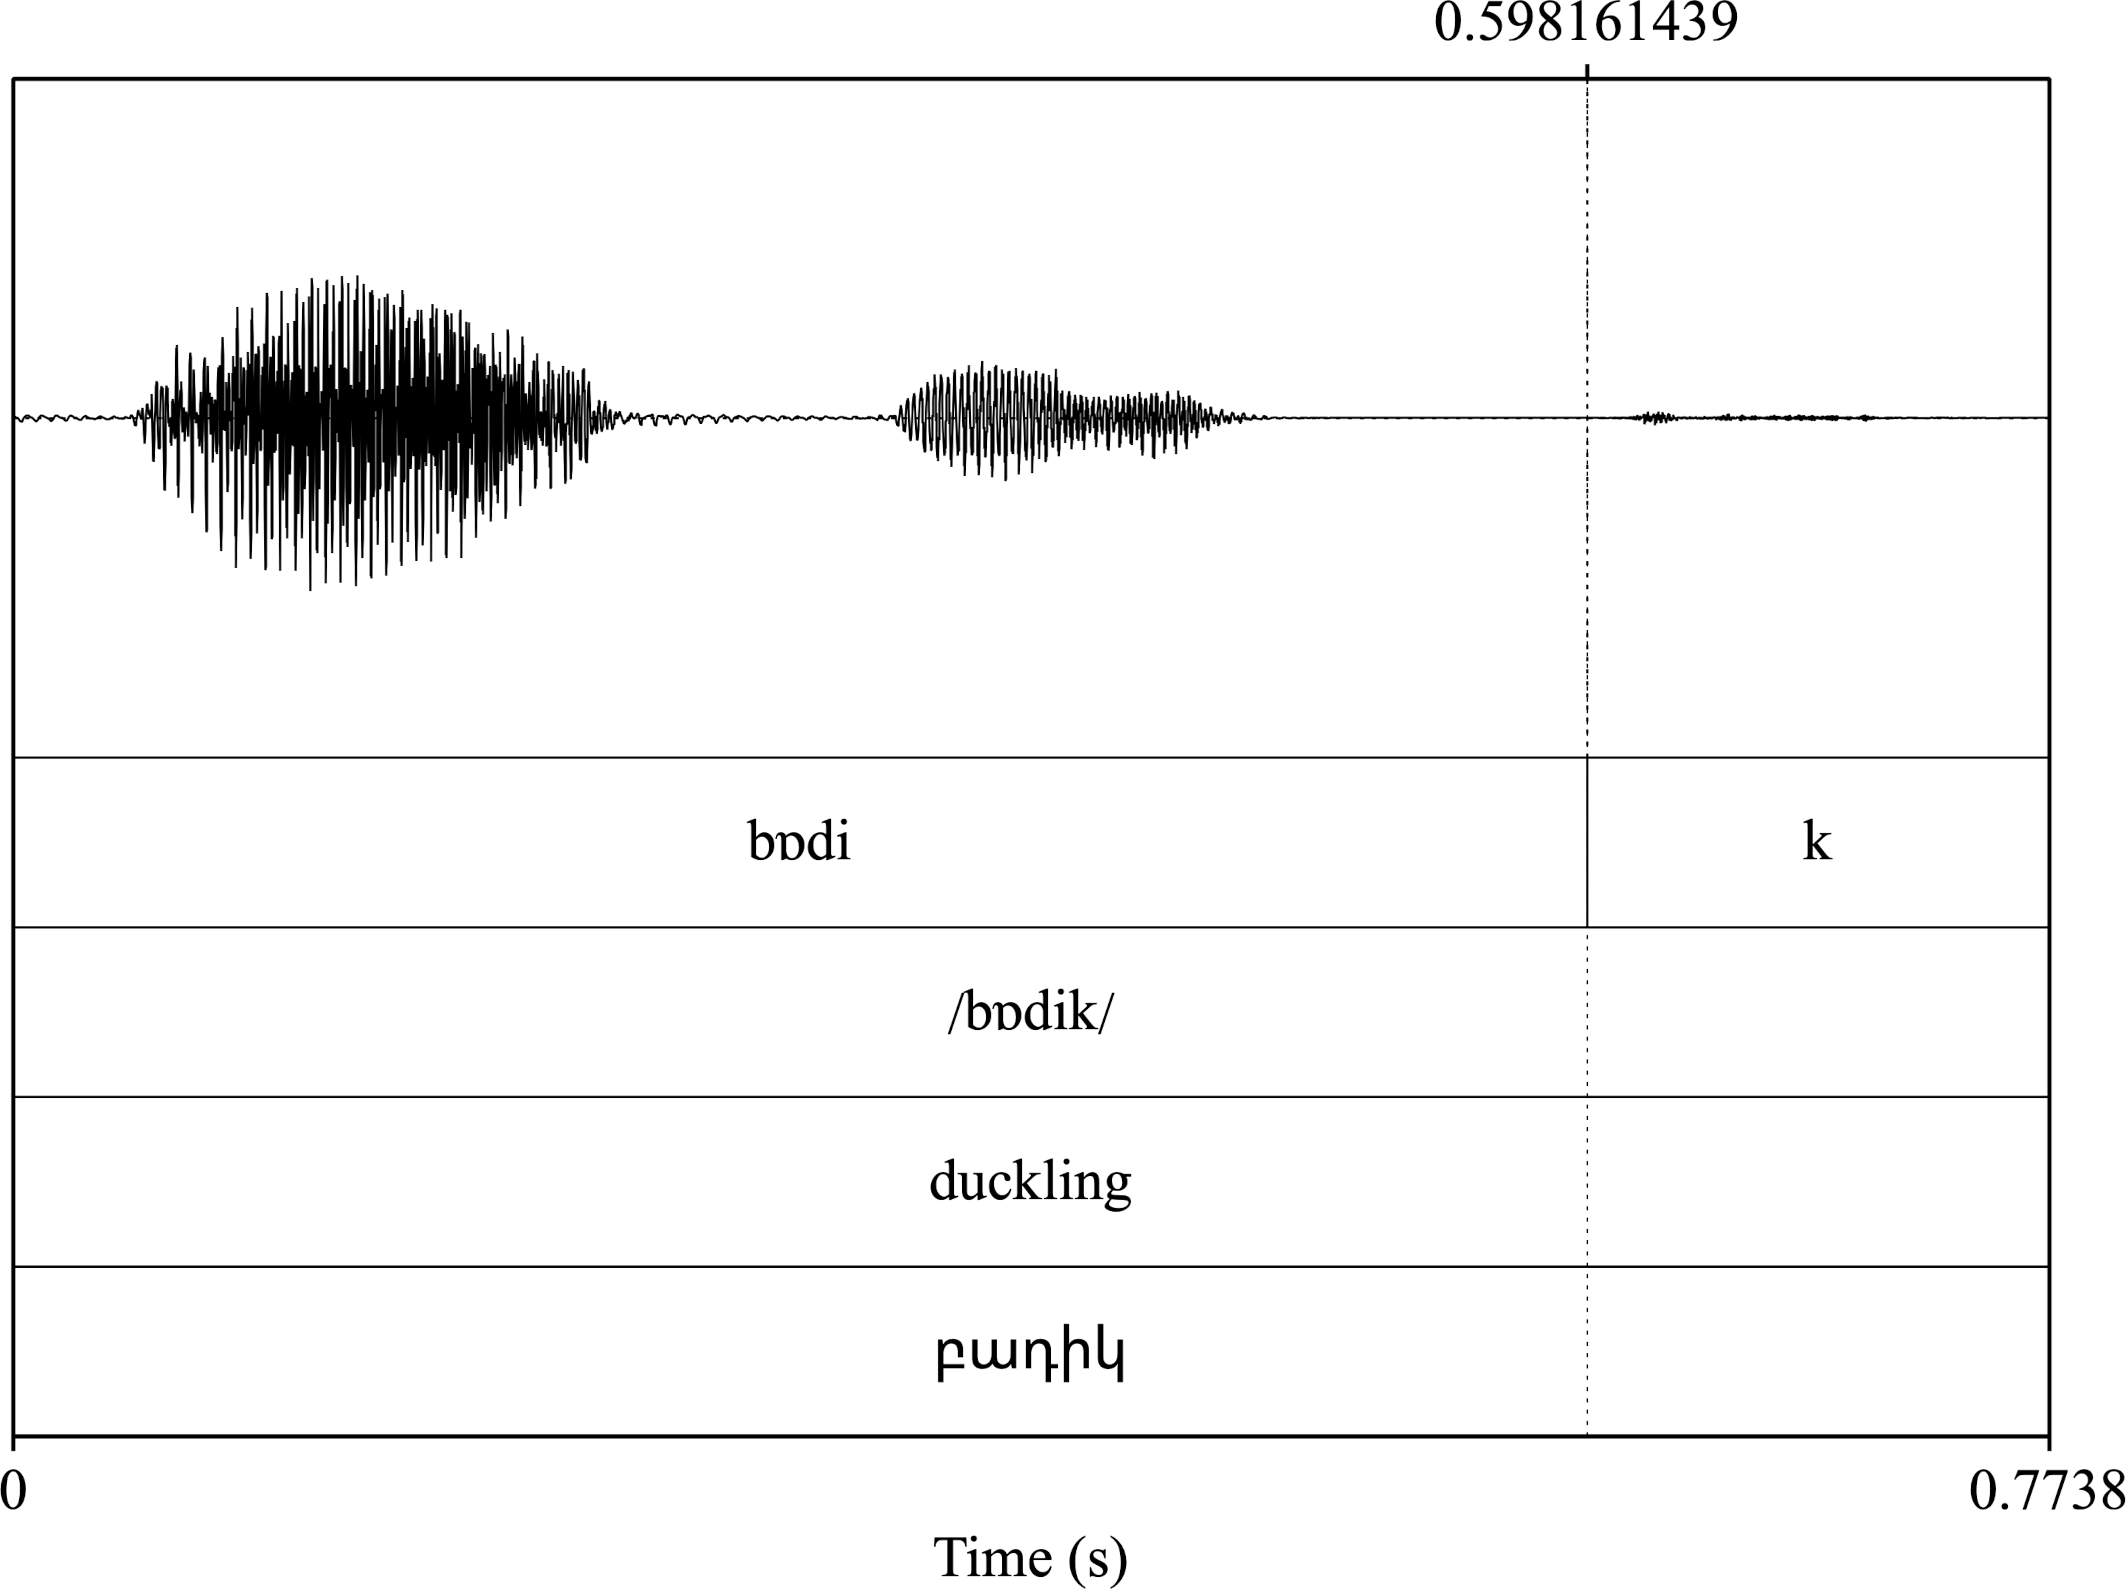
\includegraphics[width=\linewidth]{images/NK_NotEjective.png}
		\caption{Un-ejectivized final stop}
	\end{subfigure}%
	\begin{subfigure}[b]{0.5\textwidth}
		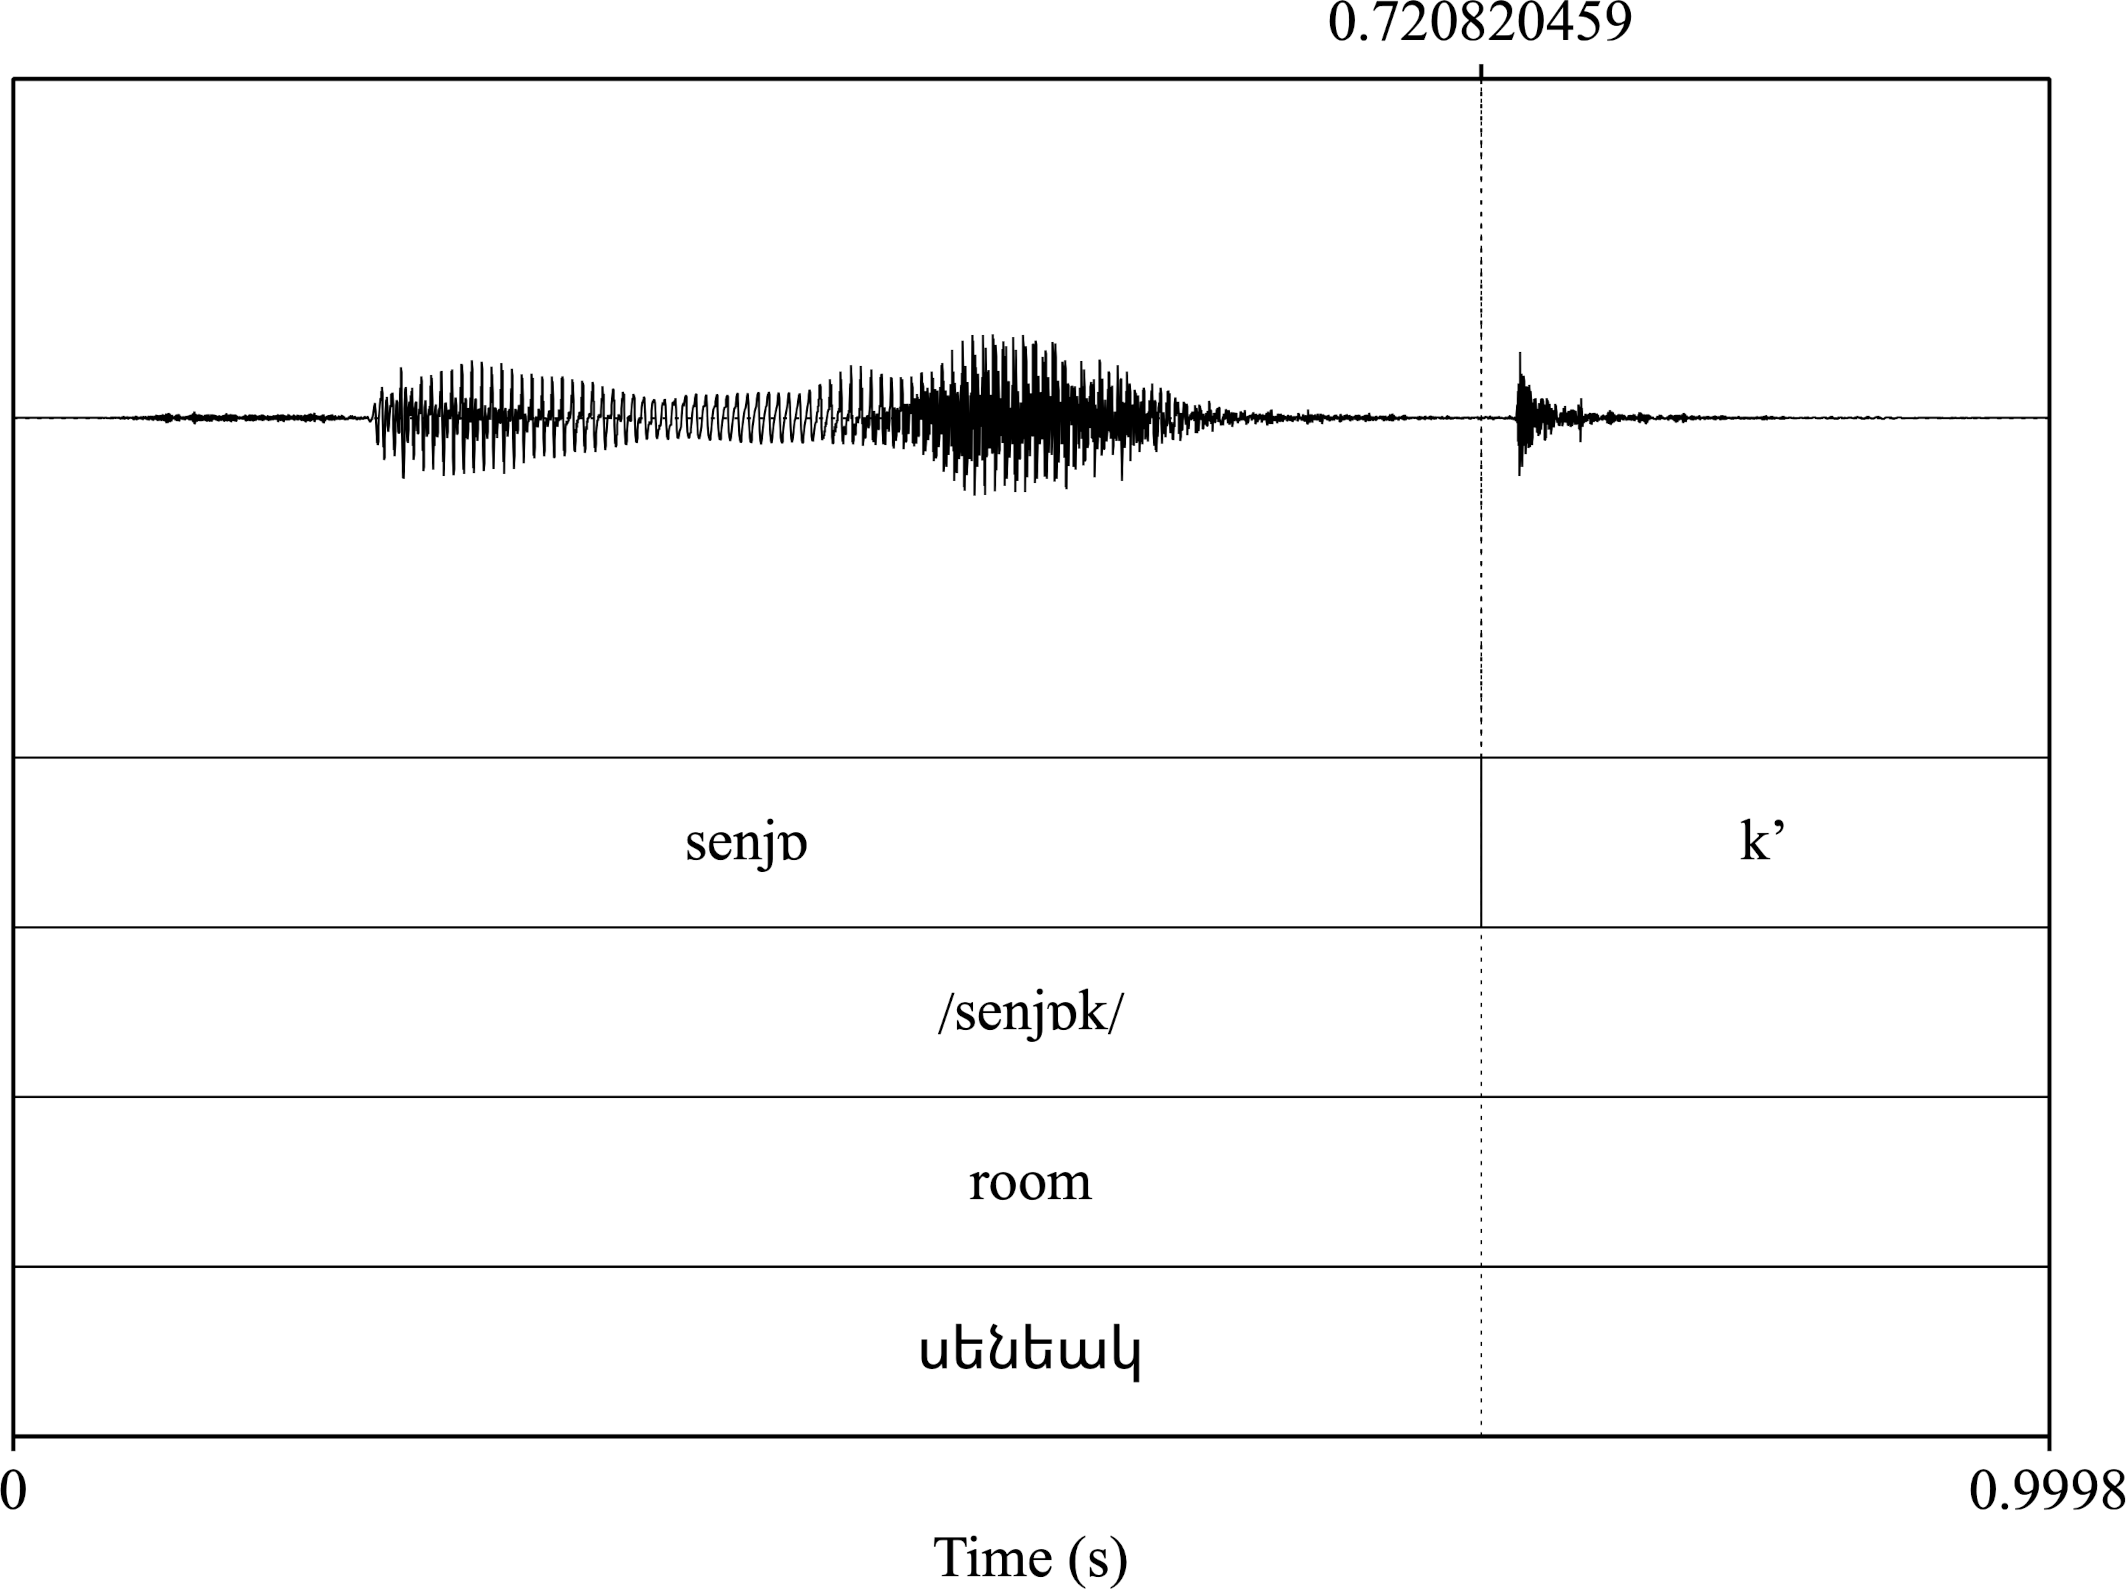
\includegraphics[width=\linewidth]{images/NK_Ejective.png}
		\caption{Ejectivized final stop}
	\end{subfigure}
\end{figure}


In general, for a given morpheme that is shared between   {\iaIA} and {\seaSEA}, the obstruents in that morpheme maintain the same laryngeal features in the two lects. That is, if a word begins   with a prevoiced stop in {\seaSE}, then it  also begins with a prevoiced stop in {\iaIA}. This correspondence is the general case. But we have encountered some morphemes where the {\iaIA} pronunciation utilizes a different laryngeal quality (Table \ref{tab:Phoon:Aspiration}). For example, the resultative participle suffix \armenian{-ած} is pronounced /{-ɑt͡s}/ in {\seaSE}, but is often pronounced as /{-ɒt͡sʰ}/ in {\iaIA} with aspiration in some speakers. NK always uses aspiration for this morpheme, while KM reports that she rarely does so. 

\begin{table}
	\caption{Unexpected aspiration in {\iaIA} from NK} \label{tab:Phoon:Aspiration}
	\fittable{\begin{tabular}{l lll l}
		\lsptoprule
		&{\seaAbbre} & {\iaAbbre} & \\\midrule
		\armenian{երգած}& {jeɾˈkʰ-ɑt͡s} & {jeɻˈkʰ-ɒt͡sʰ} &sing-{\rptcp} &  `sung'\\
		\armenian{կարդացած}& {kɑɾtʰ-ɑ-ˈt͡sʰ-ɑt͡s} & {kɒɻtʰ-ɒˈ-t͡sʰ-ɒt͡sʰ} & read-{\thgloss}-{\aor}-{\rptcp} & `read' \\
		\lspbottomrule
		\end{tabular}}
\end{table}

From AS's personal experience, the unexpected use of aspiration for the   affricate \armenian{{ծ}} /{t͡s}/ varies by speaker (Table \ref{tab:Phoon:AspirationVariable}). We speculate that this variable aspiration may be connected to variable ejectivization or glottalization of voiceless unaspirates. Variable ejectivization is reported for {\seaSE} \citep{Schirru-2012-LaryngealFeatureArmenianDialect,Seyfarth-2018-PlosiveVoicingAcousticsArmenian,ToparlakDolatian-2023-AerodynamicsarticulationwordfinalejectivesEasternArmenian}. AS likewise finds variable ejectivization for /{t͡s}/.
We speculate that what we report as aspiration might instead be a reflex of ejectivization. More data is of course needed.


\begin{table}
	\caption{Unexpected but variable aspiration of affricate /t͡s/ in {\iaIA} from NK\label{tab:Phoon:AspirationVariable}}
	\begin{tabular}{lll l}
		\lsptoprule
		&{\seaAbbre} & {\iaAbbre} & \\\midrule
		\armenian{ծնուել}& {t͡sənˈvel} & {t͡sənˈvel}$\sim${t͡sʰənvel} & `to be born'\\
		\armenian{գործածել}& {ɡoɾt͡sɑˈt͡sel} & {ɡoɻt͡sɒˈt͡sel}$\sim${ɡoɻt͡sʰɒˈt͡sʰel} & `to use' 
		\\ \lsptoprule
	\end{tabular}
\end{table}


In NK's speech (and in her family's), there were some words where the voiced stops were (variably) devoiced in her speech, and some where voiceless stops were (variably) voiced (Table \ref{tab:Phoon:AspirationVariable}). KM felt that such variable  voicing was more characteristic of heritage speakers in the diaspora than of speakers in Tehran. Note that these are all high-frequency words. 

\vfill
\begin{table}[H]
	\caption{High-frequency words with variable (de)voicing from NK and her family}\label{tab:Phono:Devoicing}
	\begin{tabular}{llll}
		\lsptoprule
		&{\seaAbbre}& {\iaAbbre} &  \\\midrule
		`(If) I come' & \textbf{ɡ}ɑm &\textbf{ɡ}ɒm, \textbf{k}ɒm  & \armenian{գամ}\\
		`door' & \textbf{d}ur &\textbf{d}ur, \textbf{t}ur  & \armenian{դուռ}\\
		`to put' & \textbf{d}ənel &\textbf{d}ənel, \textbf{t}ənel  & \armenian{դնել}\\
		`dance' & \textbf{p}ɑɾ &\textbf{p}ɒɻ, \textbf{b}ɑɻ  & \armenian{պար}\\
		`mouth' & \textbf{b}eɾɑn &\textbf{b}eɻɒn, \textbf{p}eɻɒn  & \armenian{բերան}\\
		`to bring' & \textbf{b}eɾel &\textbf{b}eɻel, \textbf{p}eɻel  & \armenian{բերել}\\
		`knife' & dɑnɑ\textbf{k} &dɒnɒ\textbf{k}, dɒnɒ\textbf{ɡ}  & \armenian{դանակ}\\
		`yesterday' & jeɾe\textbf{k} & eɻe\textbf{k}, eɻe\textbf{ɡ}  & \armenian{երեկ, էրեկ}\\
		`drawer' & dɑɾɑ\textbf{k} &dæɻæ\textbf{k}, dæɻæ\textbf{ɡ}  & \armenian{դարակ}\\
		\lspbottomrule
	\end{tabular}
	\label{tab:variabledevoicing}
\end{table}
\vfill\pagebreak

For such voicing differences, BV reports that using devoiced tokens like [tənel] instead of [dənel] `to put'   is the expected outcome in non-standard dialects of Iran, such as Urmia, Khoy, and Salmast \citep[34–40]{Asatryan-1962-KhoyUrmiaDialect},  Maragha \citep[83--89]{Adjarian-1926-MaraghaDialect}   and Keyvan (\armenian{Քեյվան}) \citep[187]{Baghramyan-1985-intermediatesubdialectGharadagh}. For   Tehrani {\iaIA}, such variation in devoicing may indicate the residue of dialect shifting, or possibly   a diglossic continuum between {\iaIA} and {\seaSEA}. 


\subsection{Rhotics}\label{section:phono:segmental:rhotic}
A stark difference between the two lects concerns their rhotics. {\seaSEA}   has a phonemic contrast between a flap /{ɾ}/ and a trill /{r}/. The flap is more frequent than the trill. Orthographically, the flap is represented by the grapheme \armenian{ր}, and the trill by \armenian{ռ}. Although {\iaIA}  also has a two-way rhotic distinction, the {\seaSE} flap corresponds to an {\iaIA} retroflex approximant /{ɻ}/. We contrast the two lects in Table \ref{tab:rhotic}.\footnote{The /{f}/ in `Raffi' is  variably geminated. The  /b/ in {\iaIA} `thin' is variably devoiced for NK.}


\begin{table}[p]
	\caption{Rhotic contrasts in {\seaSE} and {\iaIA}\label{tab:rhotic}}
	\resizebox{\textwidth}{!}{%
		\begin{tabular}{lllllll  }
			\lsptoprule
			&{\seaAbbre}&{\iaAbbre}&&{\seaAbbre}&{\iaAbbre}&\\
			&/{ɾ}/ &/{ɻ}/  &\armenian{ր}&/{r}/ &/{r}/ &\armenian{ռ}\\\midrule
			Initial &   {\textbf{ɾ}ɑˈfi} & {\textbf{ɻ}ɒˈfi}  & `Raffi (a name)'
			& {\textbf{r}eˈzin} & {\textbf{r}eˈzin} & `eraser' 
			\\
			&  & 				 &\armenian{Րաֆֆի}   & & &\armenian{ռեզին} 
			\\
			&&&
			& {\textbf{r}ɑzˈmik} &{\textbf{r}ɒzˈmik} & `Razmik (a name)' 
			
			\\
			&				&&&&  &\armenian{Ռազմիկ}
			\\
			Medial   & {bɑˈ\textbf{ɾ}ɑk} & {bɒˈ\textbf{ɻ}ɒk} & `thin' &   {ˈsɑ\textbf{r}ə} & {ˈsɒ\textbf{r}ə} & `cold' 
			\\
			&  &&\armenian{բարակ} &   & &\armenian{սառը}
			
			\\
			&
			{pɑˈ\textbf{ɾ}ɑp} &{pɒˈ\textbf{ɻ}ɒp} &  `available, empty'&
			{heˈ\textbf{r}u} & {heˈ\textbf{r}u} & `far'
			\\
			& && \armenian{պարապ}& 	& & 	\armenian{հեռու} 
			\\
			Final  & {ˈsɑ\textbf{ɾ}} &{ˈsɒ\textbf{ɻ}}  & `mountain' & {ˈbɑ\textbf{r}} & {ˈbɒ\textbf{r}} &`word'
			\\
			&  &	 &\armenian{սար} & & &\armenian{բառ}   
			\\
			& {ˈkɑ\textbf{ɾ}} &{ˈkɒ\textbf{ɻ}}  & `string'  &{ˈtɑ\textbf{r}}
			& {ˈtɒ\textbf{r}} & `letter'
			\\
			& &	&\armenian{կար} & & &  \armenian{տառ}  
			
			\\ \lspbottomrule\end{tabular}}
\end{table}


In general, if a word has a rhotic trill in {\seaSEA}, then it    has a trill in {\iaIA} as well. However, there were some high-frequency words where NK and other speakers preferred using a trill /r/ where {\seaSE} would use a flap /ɾ/ (Table \ref{tab:Phoon:RhoticTrillingVariable}). 

\begin{table}[p]
	\caption{High-frequency words that use a trill instead of an approximant}\label{tab:Phoon:RhoticTrillingVariable}
	\begin{tabular}{llll}
		\lsptoprule 
		&{\seaAbbre}& {\iaAbbre} &  \\\midrule
		`minute' & \textbf{ɾ}ope& \textbf{r}ope&  \armenian{րոպէ}  \\
		`war'& pɑte\textbf{ɾ}ɑzm & pɒte\textbf{r}ɒzm& \armenian{պատերազմ} \\  
		\lspbottomrule
	\end{tabular}
	\label{tab:trill not retro}
\end{table}

Some high-frequency words have a rhotic in {\seaSEA}, but the rhotic is optionally deleted in {\iaIA} (Table \ref{tab:Phoon:LossRhotic}).  The loss of the rhotic here may be related to the loss of rhotics in the perfective converb (\S\ref{section:morphophono:auxiliary}). 

\begin{table}[p]
	\caption{High-frequency words that lose a rhotic in {\iaIA}} \label{tab:Phoon:LossRhotic}
	\begin{tabular}{llll}
		\lsptoprule
		&{\seaAbbre}& {\iaAbbre} &  \\\midrule
		`to go' & je\textbf{ɾ}tʰɑl,   e\textbf{ɾ}tʰɑl, & e\textbf{ɻ}tʰɒl, etʰɒl  &  \armenian{երթալ, էրթալ, էթալ}  \\
		`when'& je\textbf{ɾ}pʰ & je\textbf{ɻ}pʰ, jepʰ& \armenian{երբ} \\  
		\lspbottomrule
	\end{tabular}
	\label{tab:tap lost}
\end{table}


The {\seaSE} flap  /ɾ/ is typically spirantized in some positions, such as word-finally (\cites[\S5]{Toparlak-2019-MAArmenianPhonetics}{Seyfarth-JIPAArmenian}). The {\iaIA} retroflex approximant  sounds similar to the American English alveolar approximant [ɹ] to our ears, but more retroflex like [ɻ].  A future acoustic or articulatory study can help in determining the exact place of articulation of this rhotic. 


Cross-linguistically, it is common to find that dialects differ in the phonetic realization of rhotics \citep{LadefogedMaddieson-1996-soundsWordldsLanguage,chabot-2019-WhatsWrongRhotic}.  It is rather rare to find languages with a phonemic retroflex approximant [ɻ] \citep[28]{Arsenault-2017-RetroflexionSouthAsiaTypologicalGeneticArealPatterns}. For example,  the UCLA Phonological Segment Inventory Database (UPSID) lists only 17 out of 451 languages (3.77\%) that have the phoneme /ɻ/  \citep{MaddiesonPrecoda-1989-UpdatingUPSID}.\footnote{\url{http://menzerath.phonetik.uni-frankfurt.de/S/S0763.html}} Most of these languages are in Australia. Similar results are obtained from the PHOIBLE 2.0 database at  306 out of 3020 languages (10\%) \citep{phoible}.  For the alveolar approximant [ɹ], this segment is acoustically quite similar to [ɻ]. This sound is cross-linguistically rare as well at 60 languages (2\%) in the PHOIBLE database. This segment is found particularly in Southeast Asia and in English. 



The origins of the {\iaIA} approximant could be due to language contact with Persian. Persian has a rhotic /{r}/ whose realization varies between a trill, tap, fricative, and approximant \citep{majidi-1991-persianFarsiJIPA,rafat-2010-socioPhoneticInvestigtionRhoticPersian}.  In a study on  Persian rhotics, \citet[675]{rafat-2010-socioPhoneticInvestigtionRhoticPersian} found that when  they were realized as   approximants, the approximants sounded retroflex.\footnote{However, the role of contact is likely limited. It is a stereotype that when {\iaAbbre} speakers speak Persian, they use the approximant /ɻ/ more often than Persian speakers. Classical Armenian may have had an approximant [ɹ] \citep[1040]{Macak-2017-PhonoClassicalArmenian}, so it's possible that {\iaAbbre} keeps [ɻ] as an archaism. But we suspect that it's more likely that the {\iaAbbre} /ɻ/ is an innovation.}

There is evidence that an approximant rhotic is  attested in   other Armenian dialects of Iran. In \citeauthor{Vaux-prep-NewJulfa}'s translation of  \citet{Adjarian-1940-NewJulfaDialect}'s grammar of New Julfa (Isfahan) Armenian, Vaux uses the IPA symbol [ɹ] to transcribe the letter \armenian{{ր}} (\S 6).  \citet[195]{allen-1950-notesPhoneticsEasternArmenianSpeaker} likewise reports a speaker of New Julfa who has a retroflex fricative that he transcribes as [ɹ].  It is an open question if the Tehrani [ɻ] and New Julfa [ɹ] are articulatorily different or the same.\footnote{The sound /ɹ/ is sometimes reported elsewhere in the Turkey-Caucasus-Iran region:  queer Turkish speakers from Istanbul \citep[11]{Kontovas-2012-LubuncaHistoricaldevelopmentIstanbulQueerSlang},  and the Muslim variety of the Hamshen dialect spoken in the village of Köprücü (Hopa province, northeastern Turkey) \citep[258]{Vaux-2007-HomshetsmaBook}. The sound [ɻ] is also reported in  the Iranian language of Kumzari in Oman \citep[25]{Anonby-2015-GrammarKumzariMixedPersoArabianLanguageOman}. For Turkish, it seems that approximants are generally attested    \citep{Nichols-2016-AcousticStudyTurkishRhotic},  possibly characteristic of ``white'' Turkish women and   also found in the northeastern parts of Turkey  (Nicholas Kontovas, p.c.). But it is unclear what is the exact place of articulation,  with some sources reporting an alveolar place while others report  a retroflex place \citep[12]{Tiras-2021-DissRhoticTurkish}. } 

Although the trill is phonemic in both lects, KM reports that the {\iaIA} trill feels ``not as trilled as in Eastern.'' This suggests that the trill uses a smaller number of tongue contacts in {\iaIA} than in {\seaSE}. Coincidentally, some dialects like {\swaSWA} have lost a phonemic trill for certain communities like in Lebanon \citep[16]{Vaux-1998-ArmenianPhono}.\footnote{In Armenian dialectology, Jahukyan \citep{Jahukyan-1972-ArmenianDiaolectology}     reports feature 23 as about ``confusion between /r/ and /ɾ/ in non-preconsonantal position''  in the dialects of Kuty, Hadjin, Tabriz, Tbilisi, Burdur, and Maragha.} Some communities in Canada still maintain   weak phonemic and weak articulatory distinctions between trills and flaps \citep{Tahtadjian-2020-WesterArmenianRhoticDifferentialPhoneticStudy}. KM's intuitions thus might indicate a slow language change toward  losing the trill.{\interfootnotelinepenalty=10000\footnote{%{\added}
	Don Stilo (p.c.) suggests that such a trajectory makes sense. Given that the   modern {\iaAbbre}  rhotic pair /ɻ, r/   likely descends from  a /ɾ, r/ pair (wih a flap), it is possible that the trill is slowly simplifying to become a flap.}}


\subsection{Other consonants}\label{section:phono:segmental:other cons}\largerpage
For completeness, we provide the rest of the consonantal inventory of {\iaIA} in Table \ref{tab:other consonants}. To our knowledge, the phonological properties of these remaining consonants do not differ between {\seaSE} and {\iaIA}.\footnote{%{\added}
	Don Stilo (p.c.) reports that the fricative /h/ of {\seaAbbre} and {\iaAbbre} sounds like a voiced form [ɦ]. We are not sure if this impression is accurate. Instrumental work on {\seaAbbre} reports that the fricative is generally a voiceless [h], but it has a voiced variant [ɦ] when intervocalic \citep[182--184]{Khachatryan-1988-ArmenianPhono}. In Armenian dialectology, early work by Adjarian (\citealt{Adjarian-1911-DialectologyBook}, translated in \citealt{Dolatian-prep-Adjarian}) reports a (possibly phonemic) [ɦ] in some dialects in Turkey (Erzurum/Karin, Mush, Van, Şebinkarahisar, Sebastia), but not in modern-day Armenia or Iran. Adjarian does however report in later work that the dialect of New Julfa in Iran possesses the phoneme /ɦ/   \citep[\S 5]{Adjarian-1940-NewJulfaDialect},   to which Jahukyan \citep[60]{Jahukyan-1972-ArmenianDiaolectology} adds Livasian (Chaharmahal). More recent sources also report /ɦ/ in many modern Armenian varieties spoken in the Republic of Armenia: Vardenis, Ashtarak, Koghb, Ghalacha/Berdavan, and Kamo/Gaver/New Bayazet \citep[58--59]{Jahukyan-1972-ArmenianDiaolectology}, and many more in the provinces of Gegharkunik  \citep{Katvlaryan-2018-ArmenianRepublicDialectChar1Geghargunik}  and Kotayk \citep{Katvalyan-2020-DialectBook}. 
}


\begin{table}[p]
	\caption{Other consonants in {\iaIA}}
	\label{tab:other consonants}
\small\tabcolsep=.66\tabcolsep\resizebox{\textwidth}{!}{%
		\begin{tabular}{ll ll ll ll}
			\lsptoprule 
			& &\multicolumn{2}{c}{Initial}&\multicolumn{2}{c}{Medial}&\multicolumn{2}{c}{Final}\\
			\cmidrule(lr){3-4}\cmidrule(lr){5-6}\cmidrule(lr){7-8}
			\armenian{մ} &
			/{m}/ 
			&  {ˈ\textbf{m}ɒɻtʰ} &  `man'
			
			&  {mɒˈ\textbf{m}-it͡sʰ} & `mom-{\abl}'
			
			&{dəˈɻɒ\textbf{m}} &  `Arm. dram'
			
			
			\\
			&
			&   &\armenian{մարդ}
			
			&    & \armenian{մամից}
			
			&  &  \armenian{դրամ}
			
			
			\\
			\armenian{ն} &
			/{n}/ 
			& {ˈ\textbf{n}ɒv}  &`ship'
			& {kʰəˈ\textbf{n}el}  &`to sleep'
			& {mɒˈt͡su\textbf{n}}  & `yogurt'
			\\
			&
			&    &   \armenian{նաւ}
			&    &  \armenian{քնել}
			&    & \armenian{մածուն}
			\\	\midrule 
			\armenian{ֆ} &
			/{f}/ 
			& {\textbf{f}ɒtʰiˈmɒ} &`Fatima'
			& {ɻɒˈ\textbf{f}i} &  `Raffi (name)'
			&{ˈkʰe\textbf{f}}&`party, mood'
			\\
			&
			
			&  &   \armenian{Ֆաթիմա}
			&  & \armenian{Րաֆֆի}
			&&\armenian{քէֆ}
			\\
			\armenian{ւ, վ} &
			/{v}/
			& {\textbf{v}oɾˈteʁ} &  `where'
			& {təˈ\textbf{v}oʁ} &   `giver'
			& {veˈɻe\textbf{v}} & `up'  
			\\
			&
			&   & \armenian{որտեղ}
			&  &\armenian{տուող}
			&   &\armenian{վերեւ}
			\\
			\armenian{ս} &
			/{s}/ 
			& {\textbf{s}iˈɻel} & `to love'
			& {ɒˈ\textbf{s}el} &  `to say'
			& {pɒˈkɒ\textbf{s}} & `missing'
			\\
			&
			
			&  & \armenian{սիրել}
			&   &\armenian{ասել}
			&   &\armenian{պակաս}
			\\
			\armenian{զ} &
			/{z}/
			& {ˈ\textbf{z}ɒŋɡ} &  `bell'
			& {ɒ\textbf{z}ɒˈtel} & `to free'
			& {ˈkʰe\textbf{z}} &  `you.{\dat}.{\sg}'
			\\
			&
			
			&  &\armenian{զանգ}
			& &\armenian{ազատել}
			&  &\armenian{քեզ}
			\\
			\armenian{շ} &
			/{ʃ}/ 
			& {ˈ\textbf{ʃ}eŋkʰ} & `building'
			&{pʰoˈ\textbf{ʃ}i}&  `dust'
			& {ˈt͡ʃɒ\textbf{ʃ}} &`food' 
			
			\\
			&
			
			&  &\armenian{շէնք}
			& &\armenian{փոշի}
			&   & \armenian{ճաշ}
			
			\\
			\armenian{ժ} &
			/{ʒ}/  
			& {\textbf{ʒ}əpˈtɒl} &  `to smile'
			&{uˈ\textbf{ʒ}eʁ}  &  `strong'
			& {ˈu\textbf{ʒ}}&`strength' 
			
			\\
			&
			
			& &\armenian{ժպտալ}
			& & \armenian{ուժեղ}
			& &\armenian{ուժ}
			
			\\
			\armenian{խ} &
			/{χ}/ 
			& {ˈ\textbf{χ}ɒt͡ʃʰ} &   `cross'
			& {t͡sɒˈ\textbf{χ}el} &  `to sell'
			& {ˈme\textbf{χ}} & `nail'
			\\
			&
			
			& &\armenian{խաչ}
			&  & \armenian{ծախել}
			&  & \armenian{մեխ}
			\\
			\armenian{ղ} &
			/{ʁ}/ 
			&{\textbf{ʁ}ɒzɒˈɻos}& `Lazarus'
			& {u\textbf{ʁ}ɒɻˈkel} &   `to send'
			& {ˈpʰo\textbf{ʁ}} &   `money'
			\\
			&
			
			& &\armenian{Ղազարոս}
			&  &\armenian{ուղարկել}
			&  &\armenian{փող}
			\\
			\armenian{յ, հ} &
			/{h}/ 
			& {ˈ\textbf{h}ɒt͡sʰ} &  `bread'
			& {mɒ\textbf{h}ɒˈnɒl} &  `to die'
			& {ˈʃɒ\textbf{h}} & `gain'
			
			\\
			&
			
			&  & \armenian{հաց}
			&  &\armenian{մահանալ}
			&  & \armenian{շահ}
			
			\\
			\midrule 
			\armenian{լ} &
			/{l}/ &{ˈ\textbf{l}ɒv} & `good'
			&{mo\textbf{l}oɻˈvel}  &  `to go astray'
			&  {ˈɡɒ\textbf{l}}&  `to come' 
			\\
			&
			& & \armenian{լաւ}
			&   & \armenian{մոլորուել}
			&  & \armenian{գալ}
			\\
			\armenian{յ} &
			/{j}/ 
			& {ˈ\textbf{j}eɻkʰ} & `song'
			& {tɒˈ\textbf{j}im} & `I give ({\subj}.{\pst})'
			&{ˈtʰe\textbf{j}}& `tea'
			\\
			&
			
			& &\armenian{երգ}
			&  & \armenian{տայիմ}
			& &\armenian{թէյ}
			\\
			\lspbottomrule 
		\end{tabular}}
\end{table}

The nasal /n/ becomes [ŋ] before velar stops /k, kʰ, ɡ/ (Table \ref{tab:Phono:nasalAssimilation}).

\begin{table}
	\caption{Examples of nasal place assimilation}\label{tab:Phono:nasalAssimilation}
	\begin{tabular}{lllll}
		\lsptoprule
		/zɒnɡ/ & $\rightarrow$ & ˈzɒŋɡ & `bell' & \armenian{զանգ}\\
		/menkʰ/ & $\rightarrow$ & ˈmeŋkʰ & `we' & \armenian{մենք}\\
		/tsʰɒnkɒnɒl/ & $\rightarrow$ & tsʰɒŋkɒˈnɒl & `to wish' & \armenian{ցանկանալ}\\
		\lspbottomrule
	\end{tabular}
\end{table}

In addition to the above consonantal phonemes, {\iaIA} has a surface glide [{w}] that is used to repair vowel hiatus (\ref{sent:Phono:Winsert}). This glide is discussed in \S\ref{section:morphophono:morphophono:vowel hiatus}. It is not a contrastive or phonemic segment.

\begin{exe}
	\ex \gll /kɒˈtu =e-m/ $\rightarrow $ [{kɒ.ˈtu.wem}]
	\\
	cat ={\auxgloss}-1{\sg}
	\\
	\trans	`I am a cat.'\label{sent:Phono:Winsert}
	\\
	\armenian{Կատու եմ։}
	
\end{exe}	

\subsection{Vowel inventory}\label{section:phono:segmental:vowel}
The vowel inventory is largely the same in both lects. We provide the basic vowel inventory in the two lects in Table \ref{tab:vowel inventory}. Most occurrences of the schwa are unwritten  in the orthography for {\seaSEA}. 


\begin{table}
	\caption{Vowel inventory across the lects\label{tab:vowel inventory}}
	\begin{tabular}{lllllll}
		\lsptoprule     Grapheme&\multicolumn{2}{c}{Phoneme} &\multicolumn{4}{l}{Example} \\
		&{\seaAbbre} &{\iaAbbre}& {\seaAbbre} &{\iaAbbre} &&\\\midrule
		\armenian{ա}		&/{ɑ}/&/{ɒ}/		&{t\textbf{ɑ}ˈɾi} &{t\textbf{ɒ}ˈɻi} &`year'&		\armenian{տարի}		\\
		\armenian{է, ե}	&/{e}/&/{e}/	&{t͡sʰoˈɾ\textbf{e}n} &{t͡sʰoˈɻ\textbf{e}n} &`wheat'&\armenian{ցորեն}		\\
		\armenian{ի}&/{i}/&/{i}/&{ˈkʰ\textbf{i}tʰ} &{ˈkʰ\textbf{i}tʰ}  &`nose'&	\armenian{քիթ}	\\
		\armenian{օ, ո}	&/{o}/&/{o}/ &{ˈv\textbf{o}ɾ} &{ˈv\textbf{o}ɻ} &`that'&\armenian{որ}\\
		\armenian{ու} &/{u}/&/{u}/		&{ˈd\textbf{u}r} &{ˈd\textbf{u}r} &`door'&\armenian{դուռ}\\
		\armenian{ը} &/{ə}/&/{ə}/ & {ˈmɑɾtʰ\textbf{ə}} &{ˈmɒɻtʰ\textbf{ə}} &`the man' & \armenian{մարդը}\\
		& & & {ɡ\textbf{ə}ˈɾel} &{ɡ\textbf{ə}ˈɻel} &`to write'& \armenian{գրել}\\ 
		\lspbottomrule
	\end{tabular}
\end{table}

Between the two lects, the main difference is that the low back vowel   is unrounded /{ɑ}/ in {\seaSE} but rounded /{ɒ}/ in {\iaIA}. The rounding of the low vowel is likely due to contact between {\iaIA} and Persian. Persian has a phonemic low back rounded  vowel /{ɒ}/ \citep{majidi-1991-persianFarsiJIPA}.\footnote{Anecdotally, BV has sometimes heard a rounded /ɒ/ in spoken {\seaEA} in Yerevan. In modern Persian, the low back rounded vowel /ɒ/ is acoustically unstable and can approach /{ɔ}/ \citep{esfandiari-2015-vowelClassificationVowelSpacePersian,mokari-2017-acousticDescriptionFarsiVowelsNativeSpeakerTehrani,aronowMchughMolnar-2017-pilotAcousticStudyModernPersianVowelsColloquialSpeec,jones-2019-corpusPhoneticStudyContemporaryPersianVowelCausalSpeech}. In our impressions, the {\iaIA} low vowel is much lower than the Armenian /{o}/. Although more acoustic data is needed, we speculate that the {\iaIA} /{ɒ}/ is truly [{ɒ}] and not [{ɔ}]. \label{footnote persian a}} 

When the low vowel /{ɒ}/ is next to a glide     /{j}/, the low vowel is still rounded (Table \ref{tab:Phono:LowBack}), but we suspect that it is not as rounded as in other contexts. More data is needed with finer acoustic measurements and across multiple speakers.\footnote{For the word `voice', the {\iaIA} word is [d͡zen] \armenian{ձեն} while the {\seaSE} word is the cognate [d͡zɑjn] \armenian{ձայն}. NK reports that {\iaIA}s sometimes say the word [d͡zɑjn] as a type of {\seaSE} borrowing, sometimes nativized as [d͡zɒjn].}

\begin{table}
	\caption{The low  back vowel stays rounded next to glide /{j}/}\label{tab:Phono:LowBack}
	\begin{tabular}{lll}
		\lsptoprule
		{}[{ˈhɒj}]  & `Armenian person' &\armenian{հայ}\\
		{}[mɒɻˈjɒm] & `Mariam' & \armenian{Մարիամ}\\
		\lspbottomrule
	\end{tabular}	
\end{table} 

\begin{sloppypar}
{\iaIA} likewise utilizes a   low front vowel /{æ}/ as a marginal phoneme (Table \ref{tab:low front vowel}). This vowel  appears in Persian loanwords. Some of these loanwords likewise exist in {\seaSE} (sometimes via a different route, such as from Turkish). But in {\seaSE}, the loanwords are nativized with the low back vowel /{ɑ}/. In general,  the front vowel does not appear in native Armenian words, but  we did find a  few  native constructions that contain it.\footnote{The word `drawer' is [{{dɑɾɑk}}] in {\seaSE}. In {\iaIA}, bi-dialectal KM pronounces the final stop as [k], while mono-lectal NK uses [ɡ]. We suspect this is just individual-level variation within the diaspora.}
\end{sloppypar}

\begin{table} 
	\caption{Low front vowel /{æ}/ in {\iaIA}}
	\label{tab:low front vowel}
	\resizebox{\textwidth}{!}{%
		\begin{tabular}{ll lll}
			\lsptoprule
			{\iaAbbre}&&&&cf. {\seaAbbre}\\\midrule
			{æˈɻæb} &`Arab' & \armenian{արաբ}&  from Persian&{ɑˈɾɑb}\\
			{mænˈʁæl} &`grill' &\armenian{մանղալ}&  from Persian  &{mɑnˈʁɑl} \\
			{læmæˈd͡ʒun} & `lahmacun' &\armenian{լահմաջուն} & from Turkish/Persian&{lɑhmɑˈd͡ʒun}\\
			{dæˈɻæɡ} & `drawer'&\armenian{դարակ}&   native &{dɑˈɾɑk}\\
			{mæˈhæt $\sim$ ˈmæt}& `a one'&\armenian{մի հատ}& native  & {mi ˈhɑt}\\ 
			\lspbottomrule
		\end{tabular}}
\end{table}

In the Armenian script, the front  vowel /æ/ is represented as  the symbol \armenian{ա} with umlaut       in dialectological  work. Because of variation across {\iaIA} speakers, we do not adopt this symbol in our orthographic forms, but instead use  a simple \armenian{ա}.

The use of /{æ}/ is     due to contact with Persian which has a phonemic /{æ}/ vowel \citep[286]{Mahootian-2002-PersianGrammar}. Although contemporary {\iaIA} has /{æ}/ as a marginal phoneme, it is possible that earlier stages of {\iaIA} did not. \citet[368]{zamir-1982-variationStandardPersianSociolinguisticStudy} reports that his sample of {\iaIA}s did not have the phoneme /{æ}/  when they spoke Persian. Their accent of Persian was characterized by replacing the Persian /{æ}/ with a back variant. Similarly for New Julfa Armenian in Isfahan,  Adjarian \citep[\S 7]{Adjarian-1940-NewJulfaDialect} reports that in  the 1910s/1920s, /æ/ was slowly getting introduced in the speech of young Armenians. See the translation by \citet{Vaux-prep-NewJulfa}. This suggests that the introduction of /æ/ as a marginal phoneme is both recent and widespread in the Armenian dialects of Iran.\footnote{\citet[183]{allen-1950-notesPhoneticsEasternArmenianSpeaker} reports a speaker from New Julfa who only has a low vowel  without any indication of rounding or fronting. This speaker does however self-report as being heavily influenced by Yerevan {\seaSEA}. }




As an interesting diachronic fact, there are some words that are pronounced with either   [uj]  or [ju] in {\seaSEA}, but which are pronounced with [u] in {\iaIA} (Table \ref{tab:uj ju}). But this is not a general rule   because there are some words that are pronounced with [uj] or [ju] in both varieties.\footnote{%{\added}
	For {\swaAbbre}, the {\seaAbbre} [ju] sequence corresponds to [ʏ]: [t͡sʏn] `snow'. Don Stilo reports that he may have heard some {\iaAbbre} speakers use a front vowel as well [d͡zʏn]. Unfortunately, we have not been able to replicate this form with our speaker pool.}

\begin{table}
	\caption{Dialectal variation in [uj] and [ju] sequences\label{tab:uj ju}}
	\begin{tabular}{ll lll }
		\lsptoprule
		& \multicolumn{2}{l}{Changing /uj/, /ju/ or [u]}& \multicolumn{2}{l}{Keeping /uj, ju/}\\
		\midrule
		& `sister'& `snow' & 	 `color'  & `other' 		\\
		{\seaAbbre}  & [kʰujɾ]  & [d͡zjun]& [ɡujn]& [mjus]		\\
		{\iaAbbre} &  [kʰuɻ] &  [d͡zun]& [ɡujn] & [mjus]	\\
		& \armenian{քոյր}& \armenian{ձիւն} & \armenian{գոյն} & \armenian{միւս}\\ \lspbottomrule
	\end{tabular}
\end{table}

\section{Suprasegmental phonology}\label{section:phono:suprasegmental}


In general, we did not find significant differences between {\seaSE} and {\iaIA}  in terms of syllable structure (\S\ref{section:phono:suprasegmental:syllable}). There are some differences in word stress (\S\ref{section:phono:suprasegmental:stress}). Intonational differences are   salient because {\iaIA} has borrowed aspects of Persian intonation (\S\ref{section:phono:suprasegmental:intonation}).

\subsection{Syllable structure }\label{section:phono:suprasegmental:syllable}

The syllable structure of {\iaIA}  is not substantially different from that of {\seaSE} (Table \ref{tab:syllable}). In {\iaIA}, the typical syllable is at most CVCC.  Complex onsets are limited to /Cj/ clusters, and intervocalic /Cj/ clusters are usually syllabified together into the same syllable. Complex codas generally have falling sonority. The segment /{kʰ}/ can follow any type of cluster. Phonologically, this segment is an extrasyllabic appendix. 

\begin{table}
	\caption{Syllable shapes in {\iaIA}\label{tab:syllable}}
	\begin{tabular}{l ll l}
		\lsptoprule  V& {ˈu} &`and' & \armenian{ու}   \\
		CV& {ˈdu} &`you ({\nom}.{\sg})ˈ & \armenian{դու}\\
		VC& {ˈɒpʰ} &`shore' & \armenian{ափ}\\
		CVC& {ˈpʰiʁ} &`elephant' & \armenian{փիղ}\\
		CVCC& {ˈmɒɻtʰ} &`man' & \armenian{մարդ}\\
		\midrule 
		CjVCC &{ˈkjɒŋkʰ} & `life' & \armenian{կեանք}
		\\
		CV.CjVC &{seˈnjɒk }& `room' & \armenian{սենեակ}
		\\
		CVCkʰ & {ˈpetkʰ}&`need'& \armenian{պէտք}
		\\
		CVCCkʰ & {ˈkuɻt͡skʰ}&`breast' & \armenian{կուրծք}
		\\ \lspbottomrule 
	\end{tabular}
\end{table}

All the above generalizations are likewise found in {\seaSEA}. For general overviews of syllable structure in {\seaSEA}, see \citet[\S1, 3]{Vaux-1998-ArmenianPhono}. For a discussion of the final appendix \textit{{-kʰ}} in {\seaSE}, see \citet[83]{Vaux-1998-ArmenianPhono},  \citet{VauxWolf-2009-Appendix}, and \citet[\S 5]{Dolatian-2020-NLLTArmenianReduction}.

An exception to the above generalizations concerns word-initial sibilant-stop sequences. Such clusters variably undergo schwa prothesis in both {\seaSE} and {\iaIA} (Table \ref{tab:Phono:Prothesis}). In modern Eastern, the norm is for schwa prothesis to not apply. In our elicitations from {\iaIA} speakers, most cases of sibilant-stop clusters did not undergo prothesis. When a schwa is absent, the sibilant is analyzed as an extrasyllabic appendix (\cites[83ff]{Vaux-1998-ArmenianPhono}{VauxWolf-2009-Appendix}{Dolatian-prep-Schwa}). 



\begin{table}
	\caption{Schwa prothesis in sibilant-stop clusters}\label{tab:Phono:Prothesis}
	\begin{tabular}{ ll l }
		\lsptoprule
		zɡujʃ & `caution'  & \armenian{զգոյշ}\\
		stɒnɒl & `to receive' 	& \armenian{ստանալ}\\
		(ə)skəsel & `to start'& \armenian{սկսել}\\
		əzɡɒl & `to feel'& \armenian{զգալ}\\
		skizb & `beginning'& \armenian{սկիզբ}\\
		\lspbottomrule
	\end{tabular}
\end{table}



\subsection{Lexical stress}\label{section:phono:suprasegmental:stress}
{\iaIA} seems to utilize the same lexical stress system as {\seaSEA}.  For an overview of lexical stress in {\seaSEA}, see \citet[\S4]{Vaux-1998-ArmenianPhono} and \citet{Dolatian-2020-NLLTArmenianReduction}. But there are differences in irregular stress.

\subsubsection{Regular  stress}\label{section:phono:suprasegmental:stress:reg}
Within the morphological word, stress is generally final on the rightmost non-schwa vowel (\ref{sent:Phono:regStress}). This means that regular stress is  on the final syllable if that syllable has a non-schwa nucleus.  Suffixation of non-schwa suffixes triggers stress shift.\footnote{Prescriptively, the suffix \armenian{-ութիւն} (\armenian{-ություն} in {\seaSE}) is pronounced as [{-utʰjun}]. But in casual speech, the stop-glide sequence  usually  undergoes affrication.  \label{footnote utjun}} 

\begin{exe}
	\ex \label{sent:Phono:regStress}
	\begin{xlist}
		\ex \makebox[3cm][l]{{t͡ʃɒˈ\textbf{kɒt}}}\makebox[3cm][l]{`forehead'}\armenian{ճակատ}
		
		\makebox[3cm][l]{{t͡ʃɒkɒt-ɒ-ˈ\textbf{ɡiɻ}}}\makebox[3cm][l]{`destiny'}\armenian{ճակատագիր}

  
		\ex \makebox[3cm][l]{{uˈ\textbf{ɻɒχ}}}\makebox[3cm][l]{`happy'}\armenian{ուրախ}
		
		\makebox[3cm][l]{{uɻɒχ-uˈ\textbf{t͡ʃʰun}}}\makebox[3cm][l]{`happiness'}\armenian{ուրախութիւն}
	\end{xlist}
\end{exe}

Note that [ɒ-{ɡiɻ}] is the compound linking vowel {\lvgloss} and the root [ɡiɻ] `writing'. The suffix [-ut͡ʃʰun] is a nominalizer suffix. 



If the final syllable has a schwa, then stress is on the penultimate syllable (\ref{sent:Phono:regStressSchwa}). 

\begin{exe}
	\ex  \label{sent:Phono:regStressSchwa}
	\begin{xlist}
		
		\ex \makebox[3cm][l]{{t͡ʃɒˈ\textbf{kɒ}t-ə}}\makebox[5cm][l]{`forehead-{\defgloss}'}\armenian{ճակատը}
		
		\makebox[3cm][l]{}`the forehead'
		
		\makebox[3cm][l]{{t͡ʃɒˈ\textbf{kɒ}t-əs}}\makebox[5cm][l]{`forehead-{\possFsg}'}\armenian{ճակատս}
		
		\makebox[3cm][l]{}`my forehead'
		
		\makebox[3cm][l]{{t͡ʃɒˈ\textbf{kɒ}t-ət}}\makebox[5cm][l]{`forehead-{\possSsg}'}\armenian{ճակատդ}
		
		\makebox[3cm][l]{}`your forehead'
		
	\end{xlist}
\end{exe}





Besides final schwas, stress is avoided on clitics (\ref{sent:Phono:regStressClitic}).  

\begin{exe}
	\ex \label{sent:Phono:regStressClitic}
	\begin{xlist}
		
		\ex \makebox[3cm][l]{{t͡ʃɒˈ\textbf{kɒ}t=el}}\makebox[5cm][l]{`forehead=also'}\armenian{ճակատ էլ}
		
		\makebox[3cm][l]{}`also forehead'
		
		\makebox[3cm][l]{{t͡ʃɒˈ\textbf{kɒ}t=ɒ}}\makebox[5cm][l]{`forehead={\auxgloss}'}\armenian{ճակատ ա}
		
		\makebox[3cm][l]{}`is forehead'
		\ex \makebox[3cm][l]{{uˈ\textbf{ɻɒ}χ=el}}\makebox[5cm][l]{`happy=also'}\armenian{ուրախ էլ}
		
		\makebox[3cm][l]{}`also happy'	
		
		\makebox[3cm][l]{{uˈ\textbf{ɻɒ}χ=ɒ}}\makebox[5cm][l]{`happy={\auxgloss}'}\armenian{ուրախ ա}
		
		\makebox[3cm][l]{}`is happy'
		
		
	\end{xlist}
\end{exe}

If the word takes a cluster of clitics, stress stays inside the word (\ref{sent:Phono:regStressCliticCluster}). 

\begin{exe}
	\ex \label{sent:Phono:regStressCliticCluster}\begin{xlist}
		\ex \makebox[3cm][l]{{t͡ʃɒˈ\textbf{kɒ}t=el=ɒ}}\makebox[5cm][l]{`forehead=also={\auxgloss}'}\armenian{ճակատ էլ	ա}
		
		\makebox[3cm][l]{}`is also a  forehead'
		\ex \makebox[3cm][l]{{uˈ\textbf{ɻɒ}χ=el=ɒ}}\makebox[5cm][l]{`happy=also={\auxgloss}'}\armenian{ուրախ էլ	ա}
		
		\makebox[3cm][l]{}`is also happy'
	\end{xlist}
\end{exe}


\subsubsection{Irregular  stress}\label{section:phono:suprasegmental:stress:irreg}
We catalog some morphological contexts which trigger exceptional non-final stress. 


A systematic exception to final stress involves the negation prefix /{t͡ʃʰ-}/ (pronounced [{t͡ʃʰə-}] before consonants), as in Table \ref{tab:Phono:IrregStress}. In both periphrastic and synthetic tenses, the negation prefix attracts primary stress. For periphrastic tenses, the prefix is added to the auxiliary, and the auxiliary takes stress. In synthetic tenses, the prefix is added directly to the verb. The first syllable of the verb takes stress, even if the first syllable has a schwa. 

\begin{table}
	\caption{Irregular stress in negation }\label{tab:Phono:IrregStress}
	
	\begin{tabular}{lll}
		\lsptoprule
		& Positive & Negative\\\midrule
		`I am singing' & jeɻˈ\textbf{kʰ-um} e-m & ˈ\textbf{t͡ʃʰ-e-m} jeɻkʰ-um    \\
		& sing-{\impfcvb} {\auxgloss}-1{\sg}&  {\neggloss}-{\auxgloss}-1{\sg} sing-{\impfcvb}\\
		& \armenian{երգում եմ}& \armenian{չեմ երգում}\\
		\addlinespace 					
		`he  took' & veɻ-t͡sˈ\textbf{ɻ-ɒ-v} &  ˈ\textbf{t͡ʃʰə}-veɻ-t͡sɻ-ɒ-v \\
		& take-{\caus}-{\pst}-3{\sg}&{\neggloss}-take-{\caus}-{\pst}-3{\sg}\\
		& \armenian{վերցրաւ}& \armenian{չվերցրաւ}\\
		\addlinespace 				
		`he  did' & ɒˈ\textbf{ɻ-ɒ-v} &  ˈ\textbf{t͡ʃʰ-ɒ}ɻ-ɒ-v  \\
		& do-{\pst}-3{\sg}&{\neggloss}-do-{\pst}-3{\sg}\\
		& \armenian{արաւ}& \armenian{չարաւ}\\
		\addlinespace 			
		`he  fell' & əŋˈ\textbf{ɡ-ɒ-v} &  ˈ\textbf{t͡ʃʰ-ə}ŋɡ-ɒ-v  \\
		& fall-{\pst}-3{\sg}&{\neggloss}-fall-{\pst}-3{\sg}\\
		& \armenian{ընկաւ}& \armenian{չընկաւ}\\
		\lspbottomrule
	\end{tabular}
\end{table}

Negation stress is reported in {\iaIA} dialogues from \citet{ShakibiBonyadi-1995-ShortSurveyArmenianLanguageTehrani}. In HD's experience, negation stress    is likewise attested in {\swaSWA} in both synthetic and periphrastic tenses. However in {\seaSEA}, negation attracts stress in only periphrastic tenses, not synthetic \citep[77]{Margaryan-1997-ArmenianPhonology}. The fact that {\iaIA} has negation-sensitive stress may be due to language contact with Persian, where negation is a stressed prefix \citep{Kahnemuyipour-2009-SyntaxSententialStress}. 





Another morphological exception for final stress comes from ordinals (\tabref{tab:ordStressIrregu}). The ordinal suffixes /-ɻoɻtʰ, -eɻoɻtʰ/ assign stress to the previous syllable \citep[cf.][132ff]{Vaux-1998-ArmenianPhono}. For more examples, see \S\ref{section:funct:num:ord}.  When an inflectional suffix or clitic is added after the ordinal suffix, irregular stress is lost and we get regular  stress on the rightmost non-schwa and non-clitic vowel.

\begin{table}
	\centering   \caption{Irregular stress in ordinals in Iranian Armenian}
	\label{tab:ordStressIrregu}
	\resizebox{\textwidth}{!}{%
		\begin{tabular}{lllll}
		\lsptoprule 
		a. Cardinal & 	`two'          & eɻˈ\textbf{ku}                 & 2           & \armenian{էրկու}            \\
		&		`five'       & ˈ\textbf{hiŋɡ}    & 5     & \armenian{հինգ}  \\
		\addlinespace 
		b. Ordinal & 		`second'   & ˈ\textbf{jek}-ɻoɻtʰ     & 2-{\ord}   & \armenian{երկրորդ}  \\
		&	`fifth'  & ˈ\textbf{hiŋɡ}-eɻoɻtʰ   & 5-{\ord}  & \armenian{հինգերորդ}
		\\
		\addlinespace 
		c. Adding /-i/& `to the second one'   & {jek}-{ɻoɻ}ˈ\textbf{tʰ-i-n}     & 2-{\ord}-{\dat}-{\defgloss}  & \armenian{երկրորդին}  \\
		&	`to the fifth one'   & {hiŋɡ}-e{ɻoɻ}ˈ\textbf{tʰ-i-n}     & 2-{\ord}-{\dat}-{\defgloss}  & \armenian{հինգերորդին}  \\
		\addlinespace 
		d. Adding /-ə/ & 	`the second one'   & {jek}-ˈ\textbf{ɻoɻ}tʰ-ə     & 2-{\ord}-{\defgloss}  & \armenian{երկրորդը}  \\
		& 	`the fifth one'   & {hiŋɡ}-eˈ\textbf{ɻoɻ}tʰ-ə     & 5-{\ord}-{\defgloss}  & \armenian{հինգերորդը}  \\
		\addlinespace 
		e.  Adding clitic & `he is second'   & {jek}-ˈ\textbf{ɻoɻ}tʰ  =ɒ    & 2-{\ord}={\auxgloss}  & \armenian{երկրորդ ա}  \\
		&	`he is fifth'   & {hiŋɡ}-eˈ\textbf{ɻoɻ}tʰ=ɒ     & 5-{\ord}={\auxgloss}  & \armenian{հինգերորդ ա}  \\
		\lspbottomrule 
	\end{tabular}}
\end{table}

Beyond this section, we generally avoid marking stress    in order to reduce clutter. Unless otherwise stated, stress is  on the rightmost non-schwa and non-clitic vowel. 

\subsection{Prosodic phonology and intonation}\label{section:phono:suprasegmental:intonation}

Above the word, there is relatively little known about the prosodic structure of phrases and clauses in any Armenian lect (\cites[27ff]{Fairbanks-1948-PhonologyMorphoWestern}[14ff]{Johnson-1954-EastArmGrammar}{Ghukasyan-1990-WesternEasternArmenianIntonation}{ToparlakDolatian-202x-IntonationFocusMarkingWesternArmenian}{Dolatian-2022-InterfaceNuclearStressWesternArmenianTurkishPersian}).  There is however one aspect of {\iaIA} prosodic phonology which stands out from {\seaSEA}. This concerns the intonational structure of questions.  We briefly overview the main properties of {\iaIA} interrogatives, using common notation from the autosegmental-metrical tradition on intonational phonology \citep{Pierrehumbert-1980-phonologyPhoneticsEnglishIntonation,Ladd-1986-IntonationalPhrasingRecursiveProsodic,jun-2007-prosodicTypologyPhonologyIntonationPhrasing}. The recordings from this subsection can be found in the online archive.\footnote{\url{https://github.com/jhdeov/iranian_armenian}}

In   a basic SOV sentence in the present tense (\ref{example: sov dec sentence}), verbal inflection is periphrastic. The verb is in the form of the imperfective converb, and tense-agreement marking is on an auxiliary.  If the object is morphologically bare, then it carries sentential stress (nuclear stress, underlined). The auxiliary is cliticized to the bare object.\footnote{The distribution of this auxiliary is complex in {\seaSE} and {\iaIA} (\S\ref{section:morphophono:auxiliary:syntax}). For further data and discussion, see \citet{Tamrazian-1994-ArmenianSyntax,Megerdoomian-2009-ThesisBook,KahnemuyipourMegerdoomian-2011-secondcliticvP,KahnemuyipourMegerdoomian-2017-positionalDistriutionFocus}.} Declarative sentences end in falling intonation.\largerpage[2]




\begin{exe}
	\ex 
	\begin{xlist}
		\ex \textit{Declarative    SOV sentence with an auxiliary}\label{example: sov dec sentence}
		
		{%\resizebox{.85\textwidth}{!}{%
				\begin{tabular}{llllll}
					i.& {mɑɾjɑ-n}& {\uline{ɡiɾkʰ}}&={e}& {kɑɾtʰ-um}$\searrow$&({\seaAbbre})
					\\
					&\multicolumn{5}{l}{\armenian{Մարիան գիրք է կարդում։}}
					\\
					
					ii. & {mɒɻjɒ-n}&   {\uline{ɡiɻkʰ}}&={ɒ}& {kɒɻtʰ-um}$\searrow$&({\iaAbbre})
					\\
					
					& Maria-{\defgloss}&book&={\auxgloss}& read-{\impfcvb} & 
					\\
					&\multicolumn{5}{l}{`Maria is  reading books.'
					}   
					\\ 
					&\multicolumn{5}{l}{\armenian{Մարիան գիրք ա կարդում։}}
					\\
				\end{tabular} 
			}

			\ex \textit{Polar question} \label{example: sov polar sentence}
			
			{%\resizebox{.85\textwidth}{!}{%
					\begin{tabular}{llllll}
						i.& {mɑɾjɑ-n}& {\uline{ɡiɾkʰ}}$\nearrow$&={e}& {kɑɾtʰ-um}$\searrow$&({\seaAbbre})
						\\
						&\multicolumn{5}{l}{\armenian{Մարիան գի՞րք է կարդում։}}
						\\
						ii. & {mɒɻjɒ-n}&   {\uline{ɡiɻkʰ}}$\nearrow$&={ɒ}& {kɒɻtʰ-um}$\nearrow$&({\iaAbbre})
						\\
						& Maria-{\defgloss}&book&={\auxgloss}& read-{\impfcvb} & 
						\\
						&\multicolumn{5}{l}{`Is Maria reading  books?'
						}
						\\
						&\multicolumn{5}{l}{\armenian{Մարիան գի՞րք ա կարդում։}}
						\\
						
					\end{tabular} 
				}			
			\end{xlist}
			
		\end{exe}
		
		To form polar questions, the only strategy in {\seaSE} and {\iaIA} is   intonational. In {\seaSEA}, there is a significant rise in pitch on the bare object in (\ref{example: sov polar sentence}-i). The sentence ends in falling intonation \citep[cf.][]{Ghukasyan-1990-WesternEasternArmenianIntonation,Ghukasyan-1999-EasternYesNoQuestionIntonation}. In contrast in {\iaIA}, there is both a rise on the object and a sentence-final rise (\ref{example: sov polar sentence}-ii). 
		
		For illustration, Figure \ref{fig:dec polar basic eastern iranian}  shows the pitch track of the declarative sentence (\ref{example: sov dec sentence}) and its corresponding polar question (\ref{example: sov polar sentence}) in both {\seaSE} and {\iaIA}.  	The {\iaIA} recordings are from NK. The {\seaSEA} recordings are from AT. We annotate the perceived nucleus with the H* symbol, sentence-final fall with L\%, and sentence-final rise with H\%.
		
 
		
		
		As is clear, both declarative sentences end in L\%. The {\iaIA} polar question has H\%. For {\seaSE}, both the declarative and polar question   end in a L\%. The main difference is the level of pitch on the nuclear stressed word [{ɡiɾkʰ}] `book'.
		
	\vfill
	\begin{figure}[H]
		\caption{Pitch track of declarative (\ref{example: sov dec sentence}) and polar question (\ref{example: sov polar sentence})   in   {\seaAbbre}   an {\iaAbbre} \label{fig:dec polar basic eastern iranian}}
		\begin{subfigure}[b]{0.5\textwidth}
			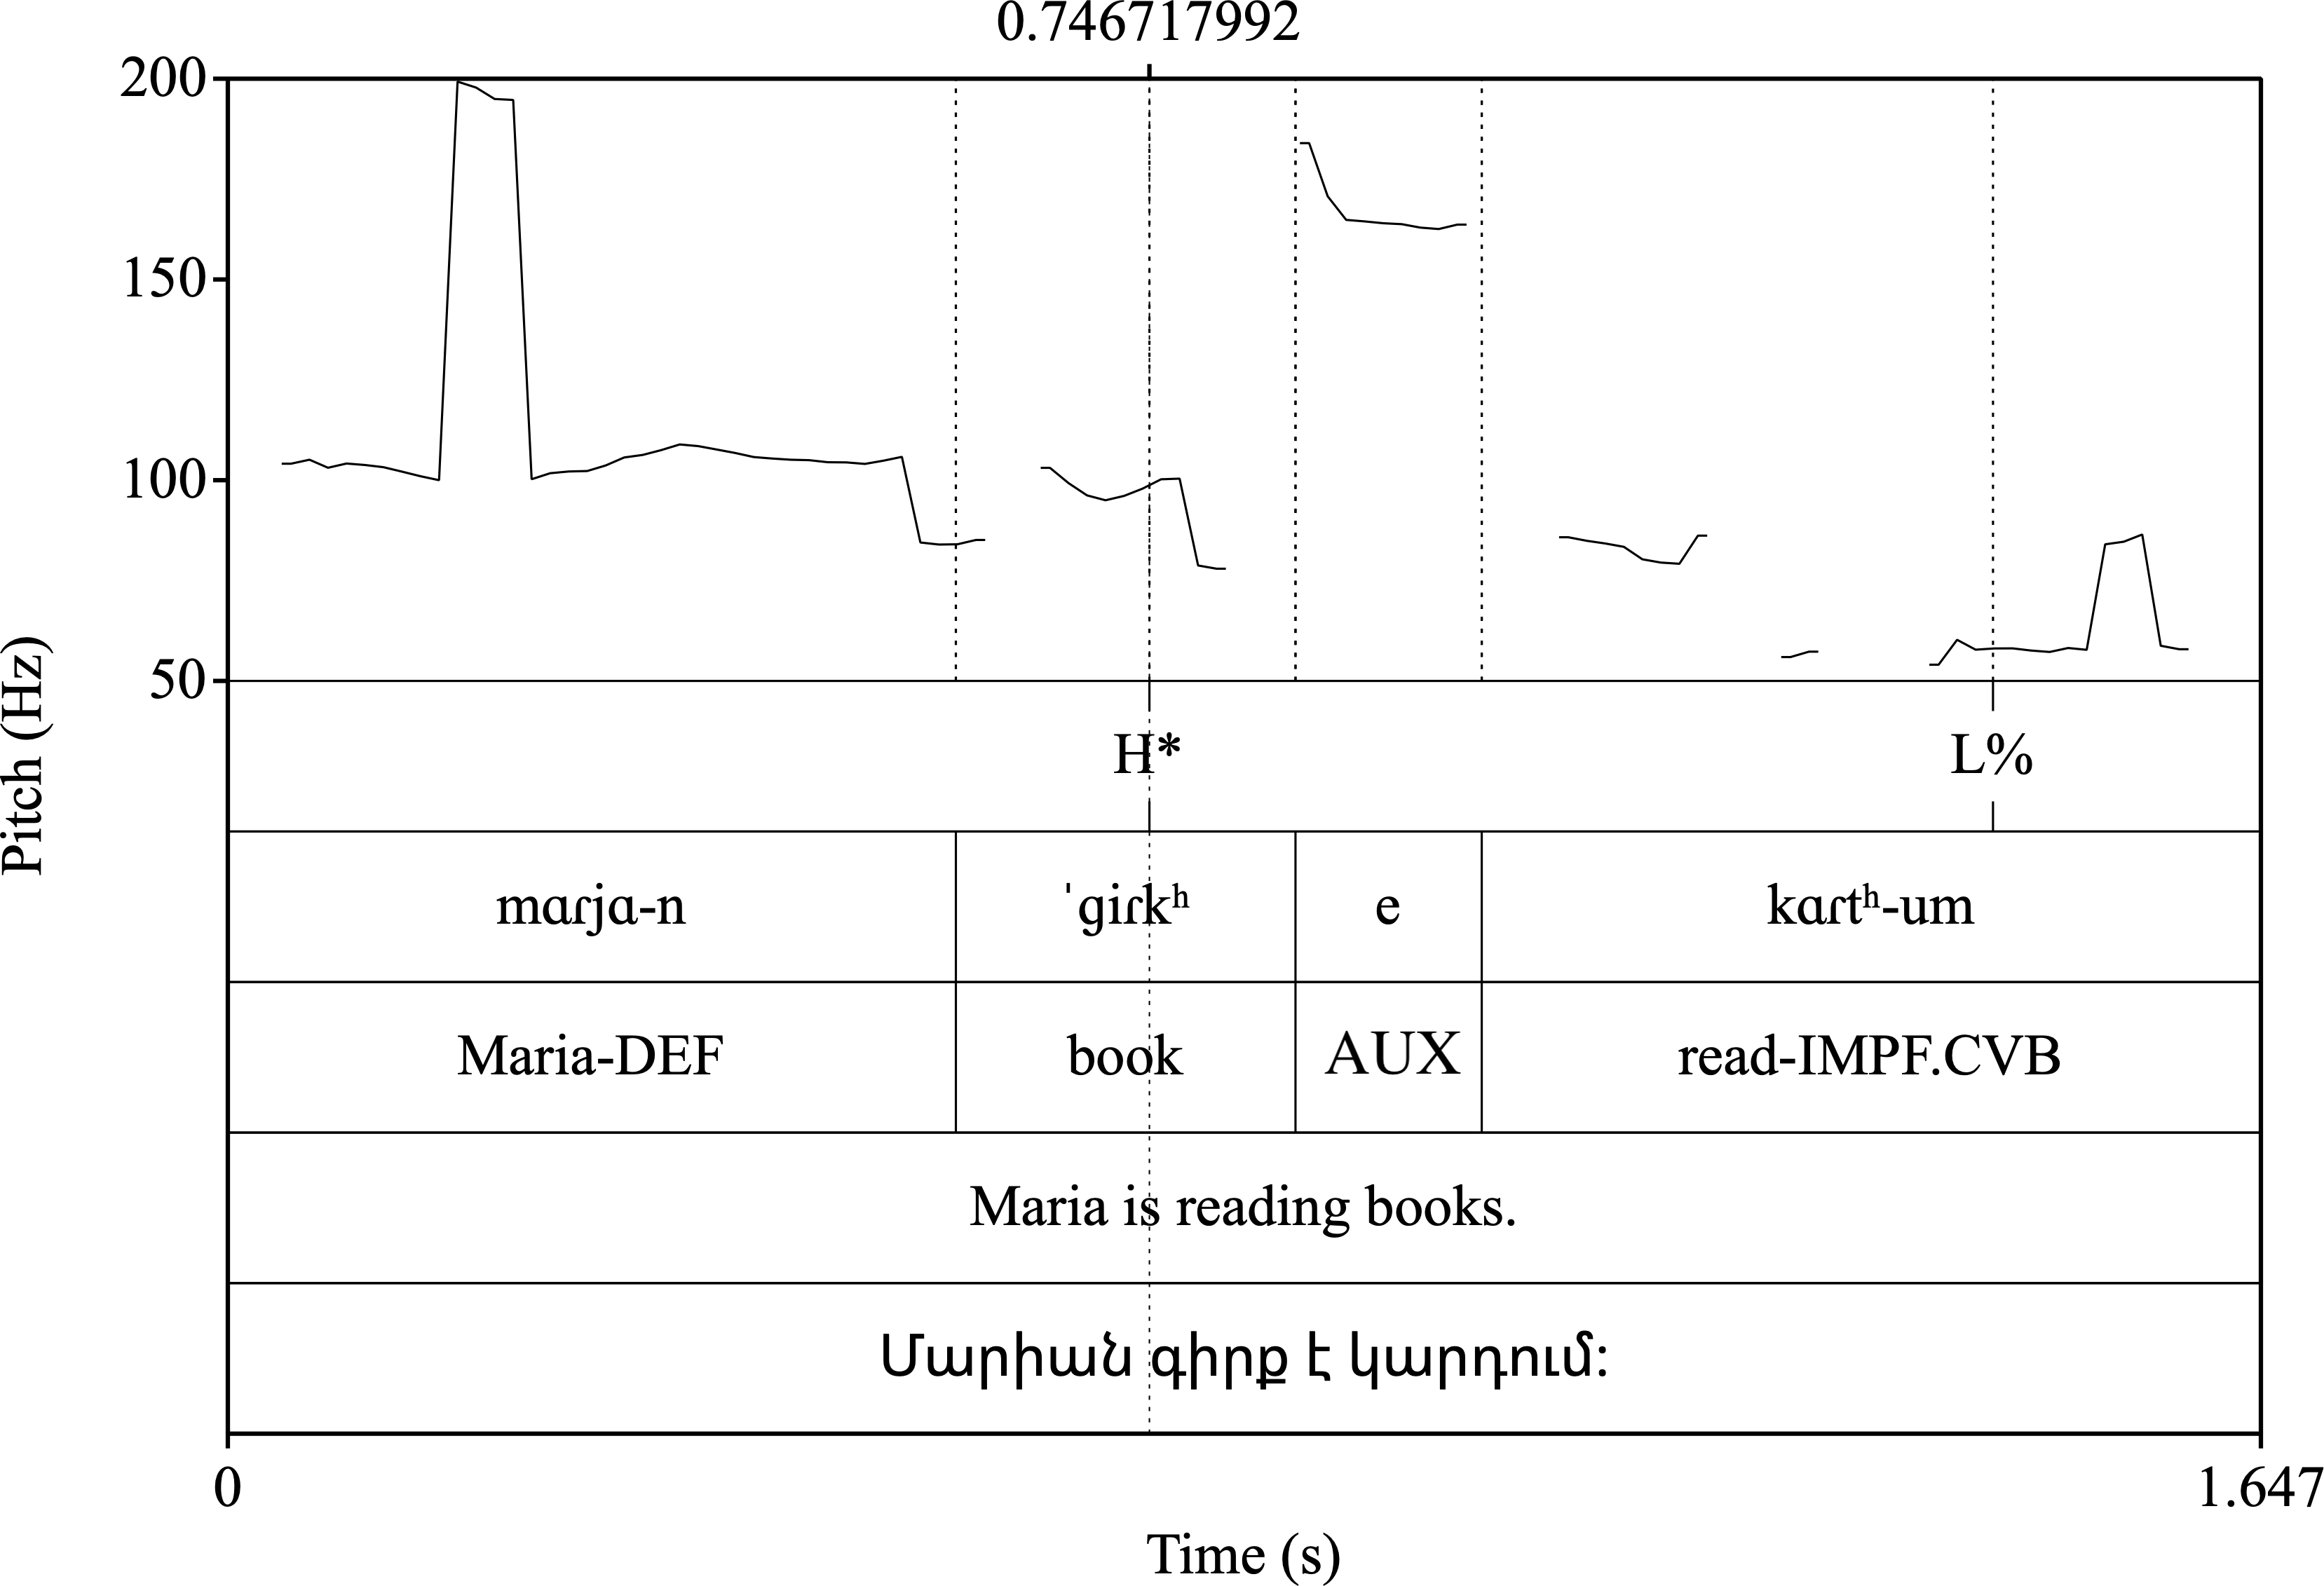
\includegraphics[width=\linewidth]{images/AT_Declarative.png}
			\caption{{\seaAbbre} declarative   with L\%}
		\end{subfigure}%
		\begin{subfigure}[b]{0.5\textwidth}
			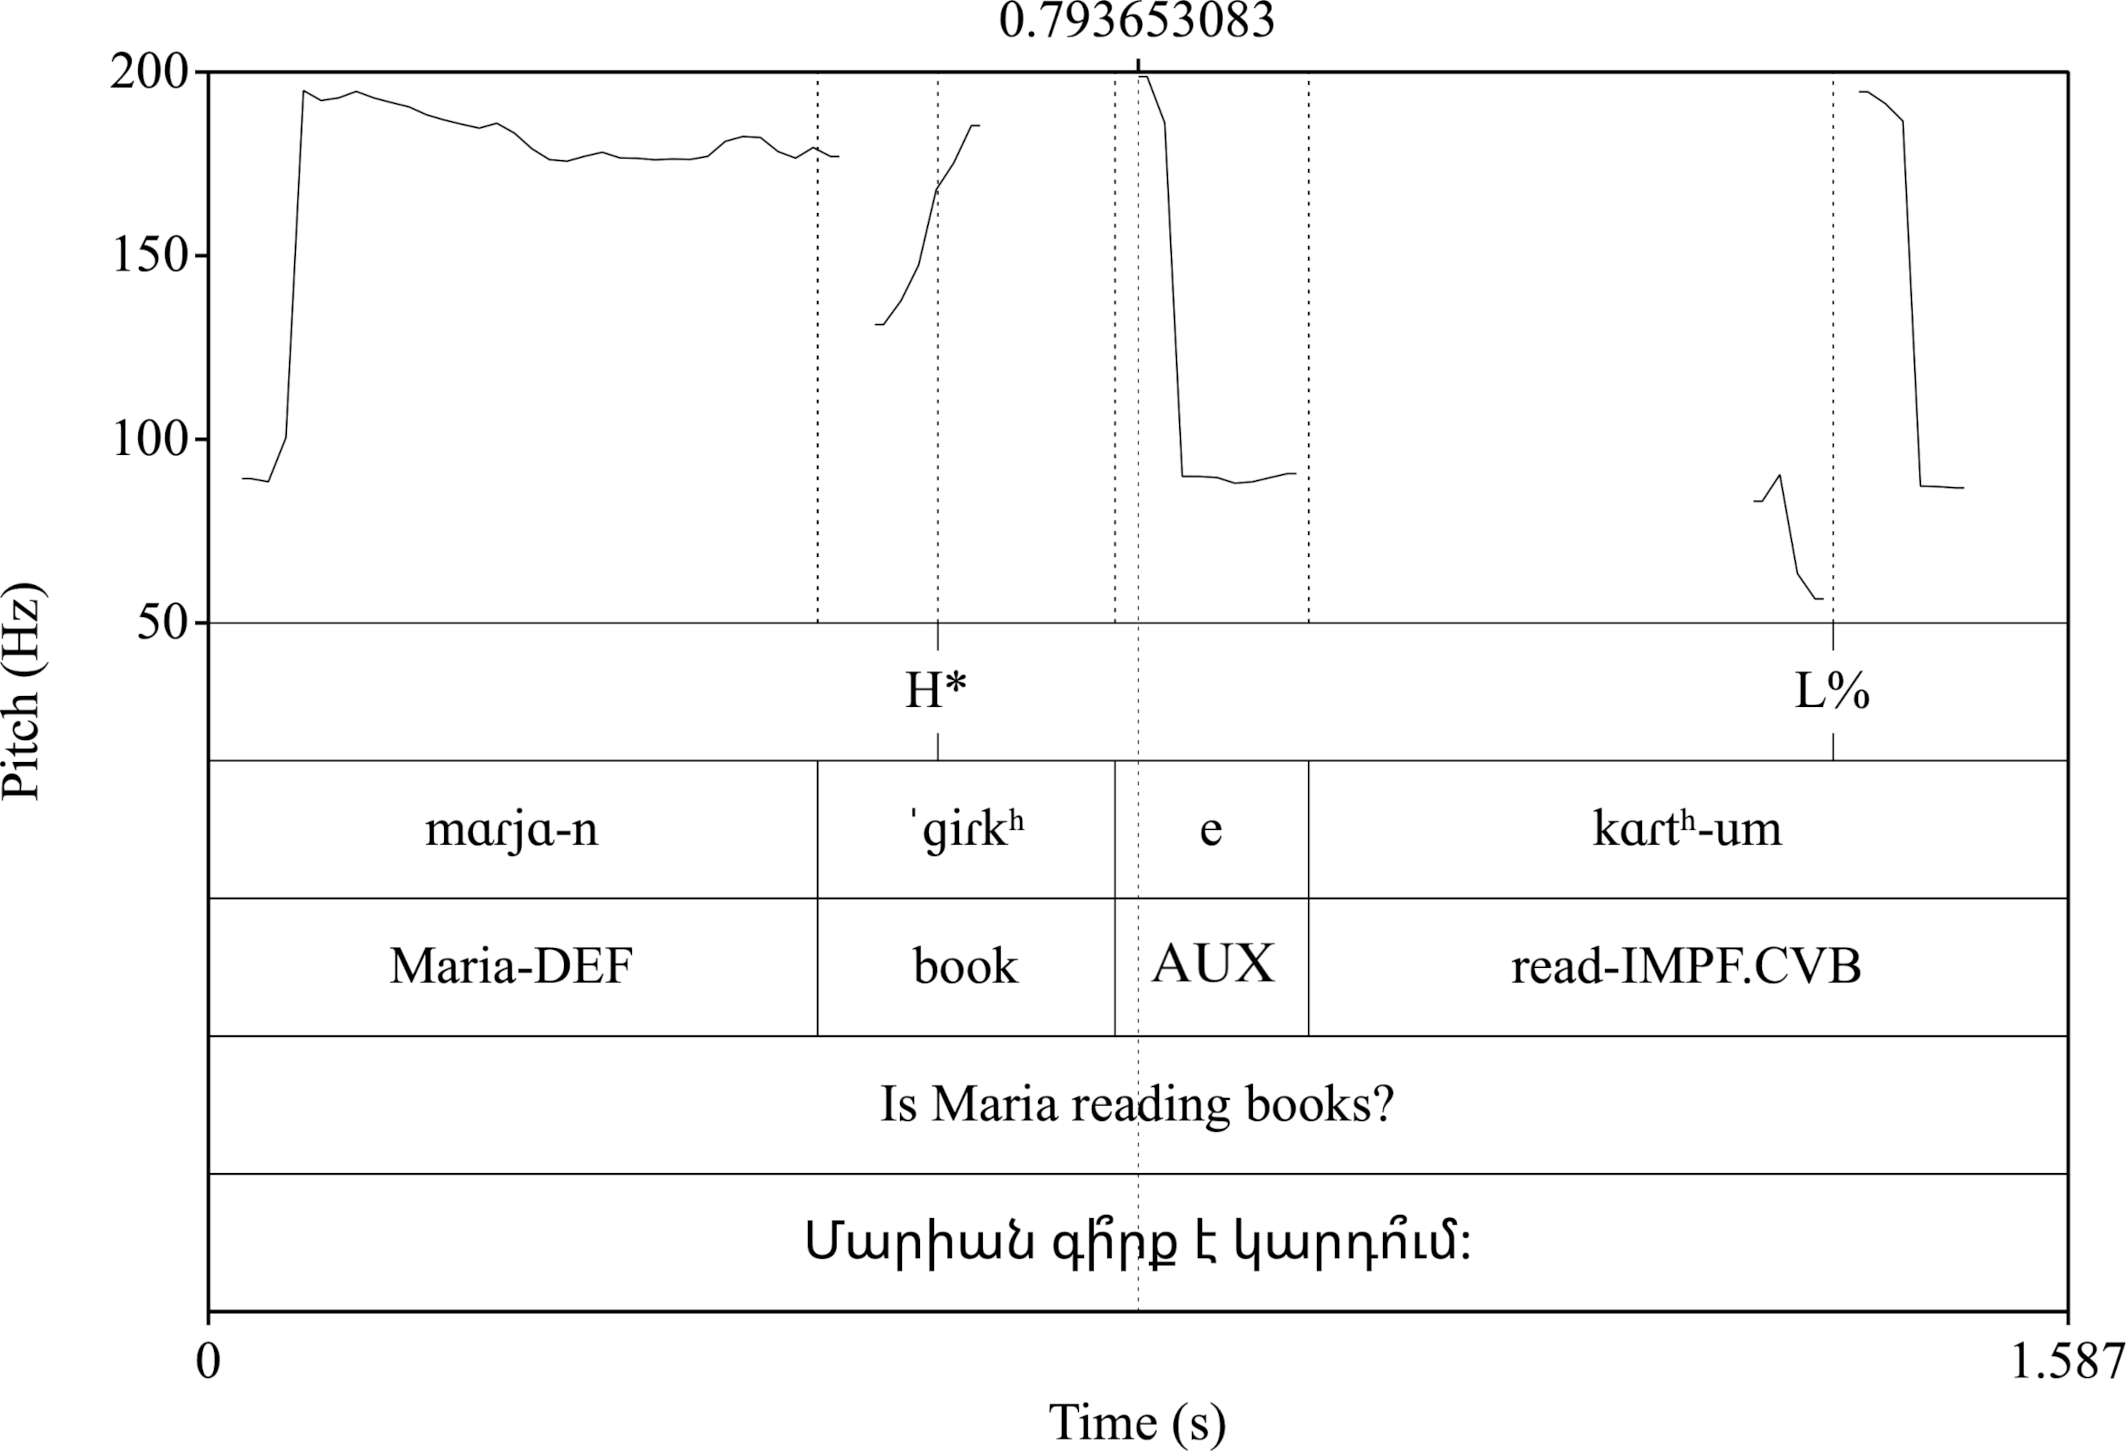
\includegraphics[width=\linewidth]{images/AT_PolarQuestion_LowTone.png}
			\caption{{\seaAbbre} polar  with L\%}
		\end{subfigure}\smallskip\\
		\begin{subfigure}[b]{0.5\textwidth}
			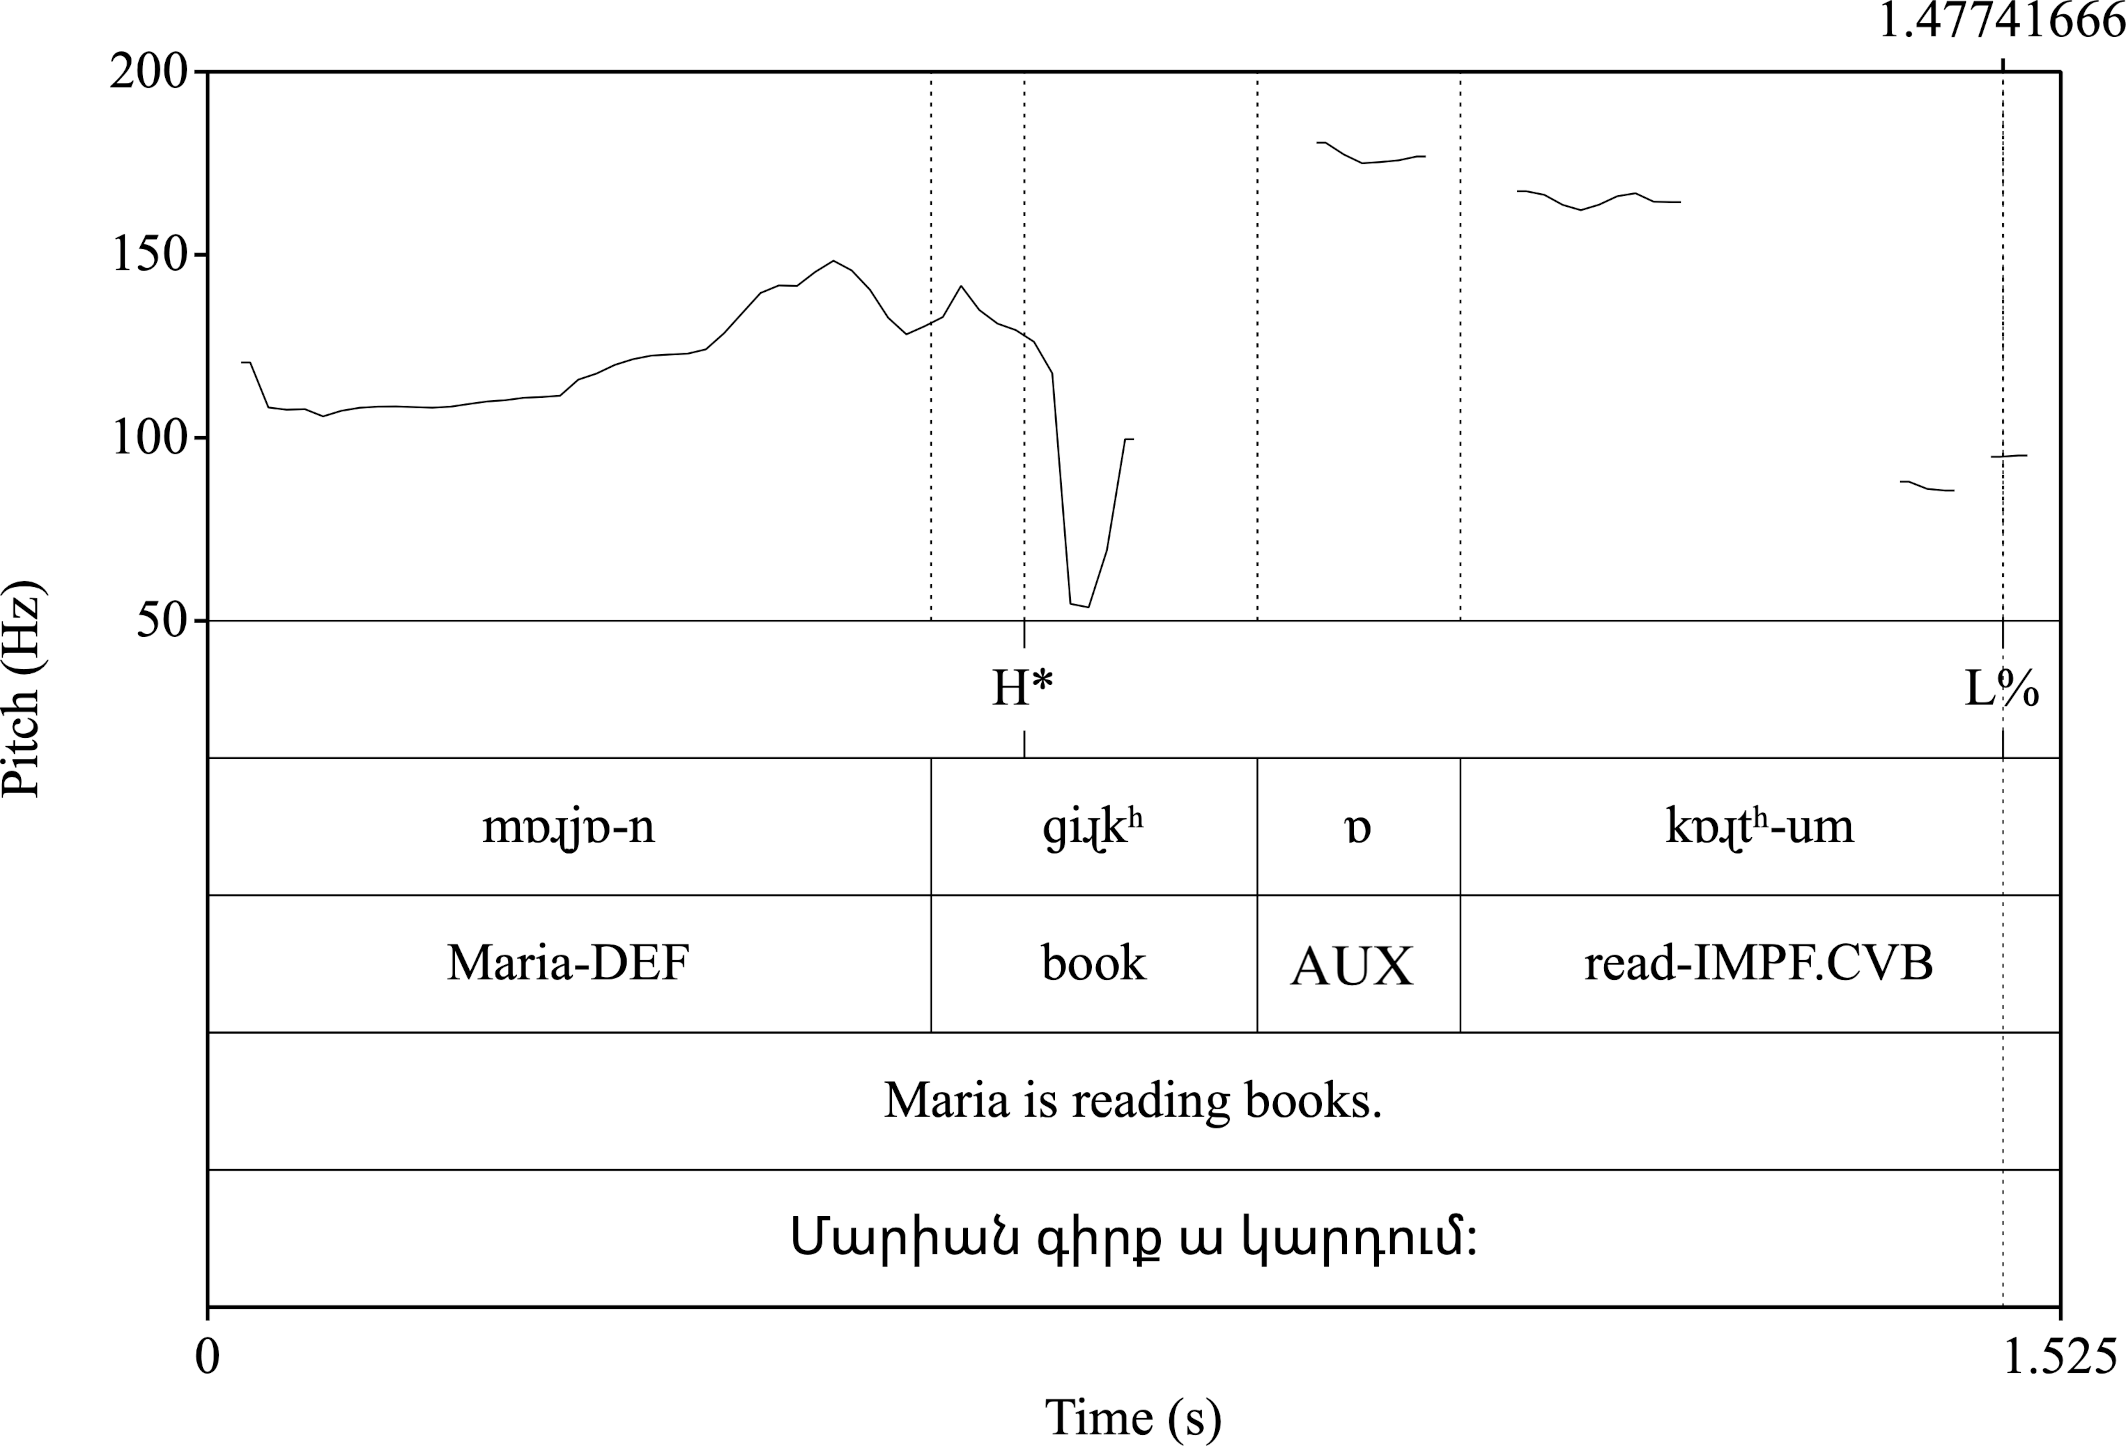
\includegraphics[width=\linewidth]{images/NK_Declarative.png}
			\caption{{\iaAbbre} declarative   with L\%}
		\end{subfigure}%
		\begin{subfigure}[b]{0.5\textwidth}
			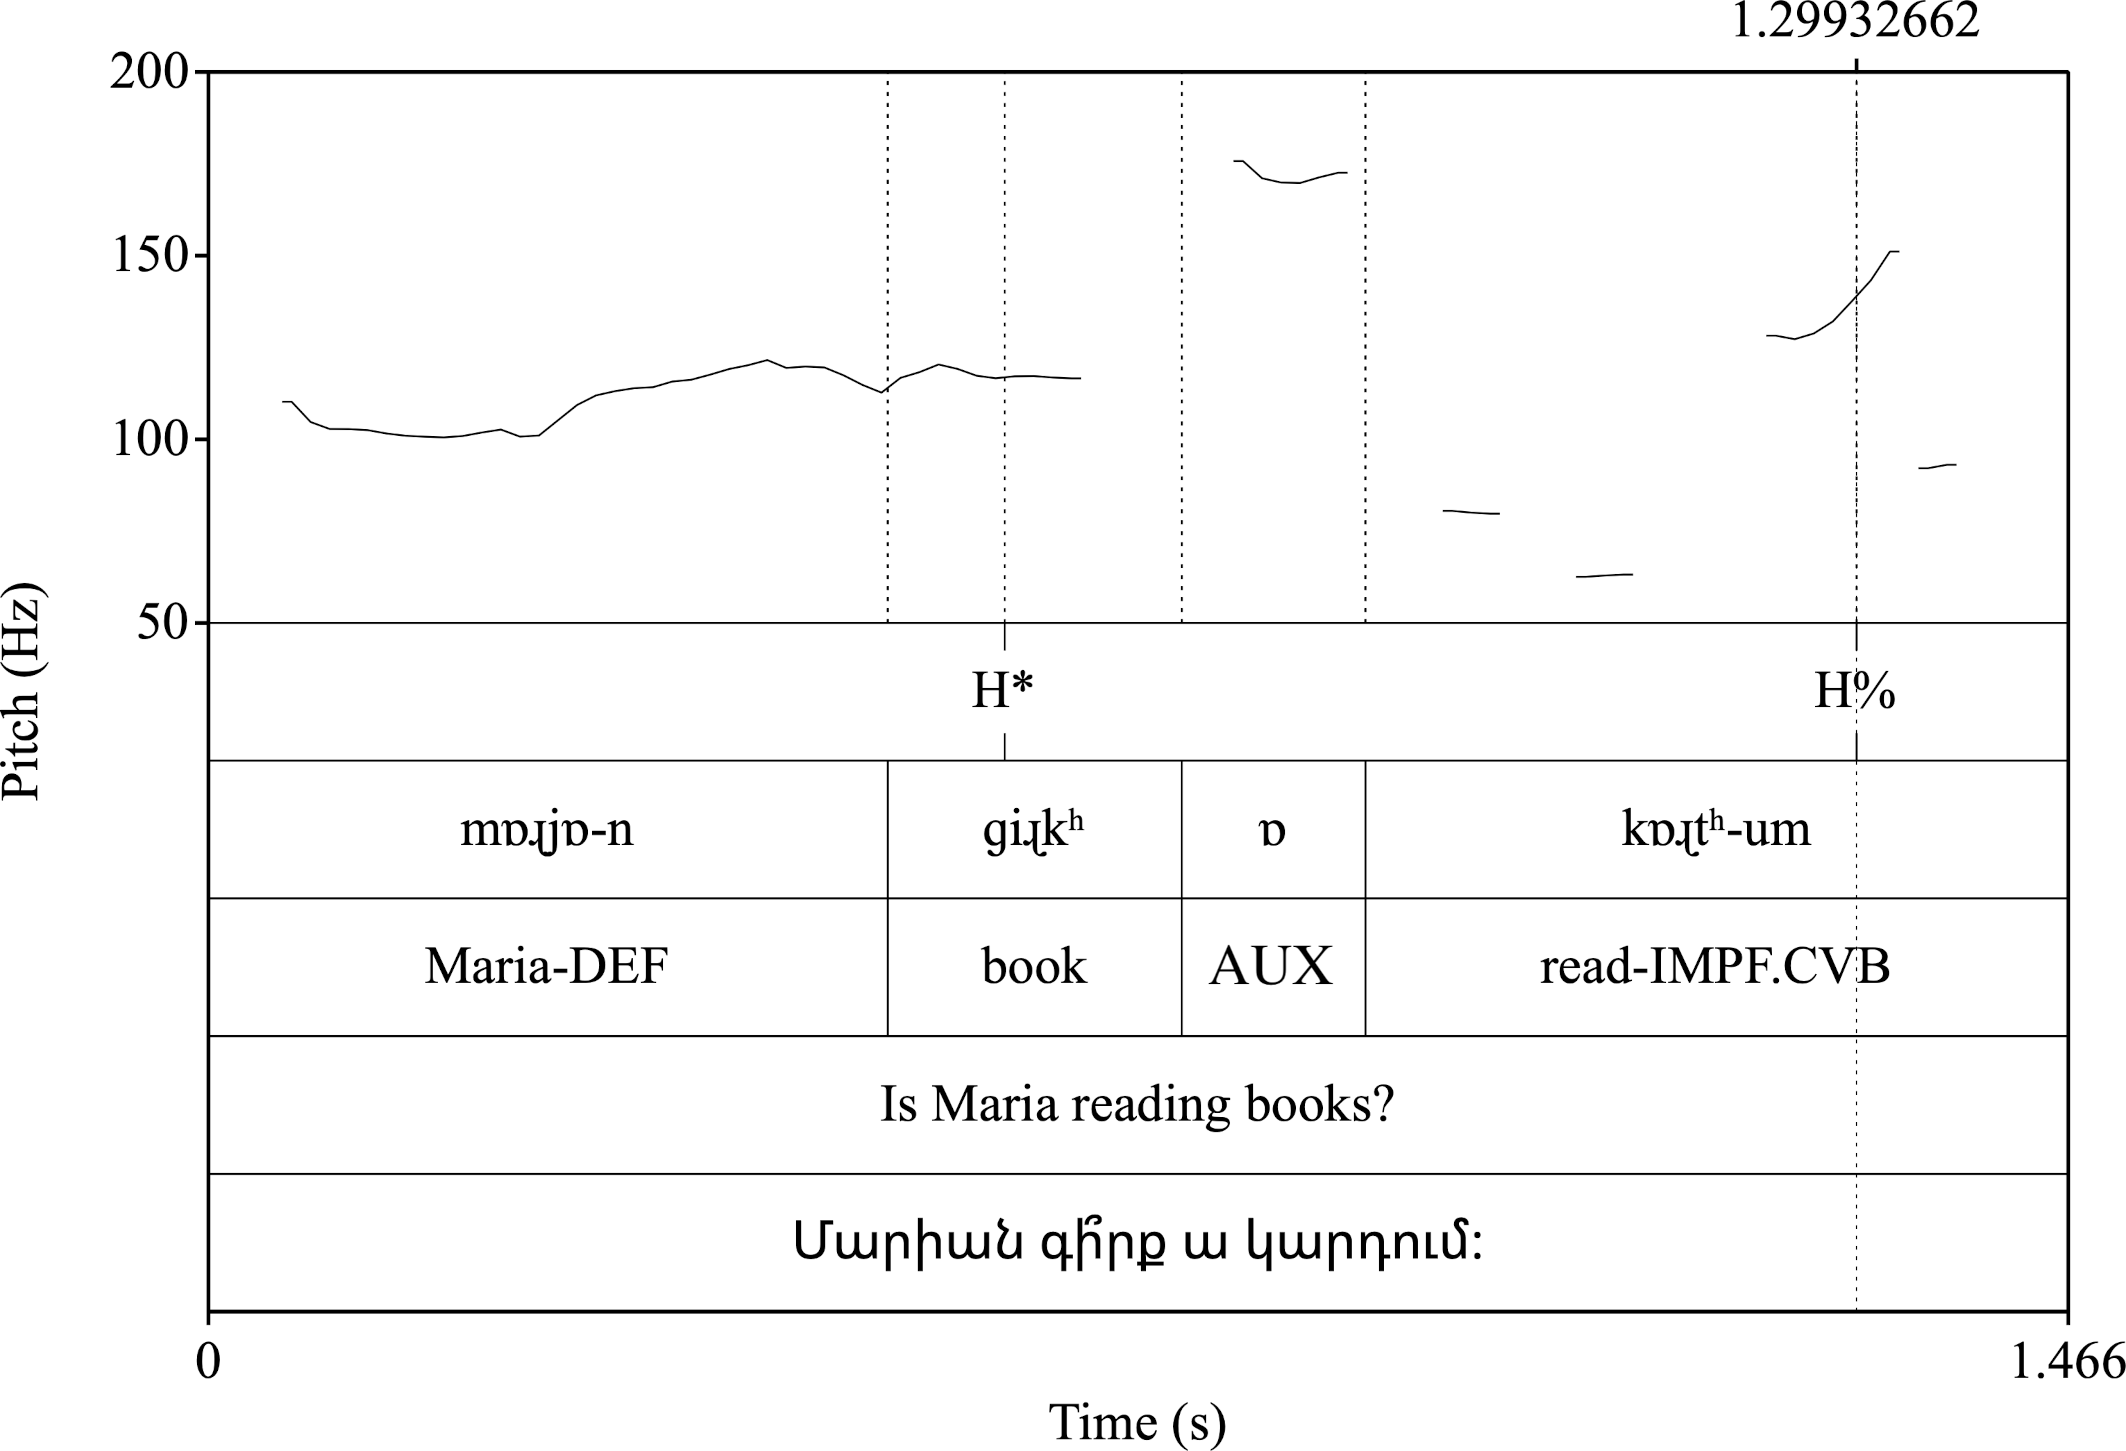
\includegraphics[width=\linewidth]{images/NK_PolarQuestion.png}
			\caption{{\iaAbbre} polar  with H\%}
		\end{subfigure}			
	\end{figure}\vfill\pagebreak
		
		The use of a sentence-final rise is likely due to two factors: one language-internal, and the other is language contact with Persian.
		
		
		In  Persian, polar questions end in a sentence-final rise as a type of Intonational Phrase boundary H\% (\citealt[111]{SadatTehrani-2007-IntonationPersian,sadat-2011-intonationPatternsInterrogativesPersian}, \citealt[55]{Mahjani-2003-PersianIntonation}). Furthermore, AS reports that some {\iaIA} speakers draw out the last syllable, i.e., they apply sentence-final lengthening. This is also reported in Persian polar questions \citep[113]{sadat-2011-intonationPatternsInterrogativesPersian}. 
		
 
		As for language-internal factors, prescriptively, {\seaSEA} uses L\% for polar questions when nuclear stress is on a non-final word. However, AT informs us that {\seaCEA} (as spoken in Yerevan) does allow a final H\%. She said that the use of this H\% is socially judged   as ``improper'' for her {\seaEA} community. We provide a pitch track in Figure \ref{fig:eastern polar H}. Another parallelism is that {\seaCEA} can also use the colloquial auxiliary [ɑ] (like {\iaAbbre}) instead of the standard [e]. 
		
 
		
		\begin{figure}
			\caption{Polar question in {\seaSE} (\ref{example: sov dec sentence}-i) with optional H\% }
			\label{fig:eastern polar H}
			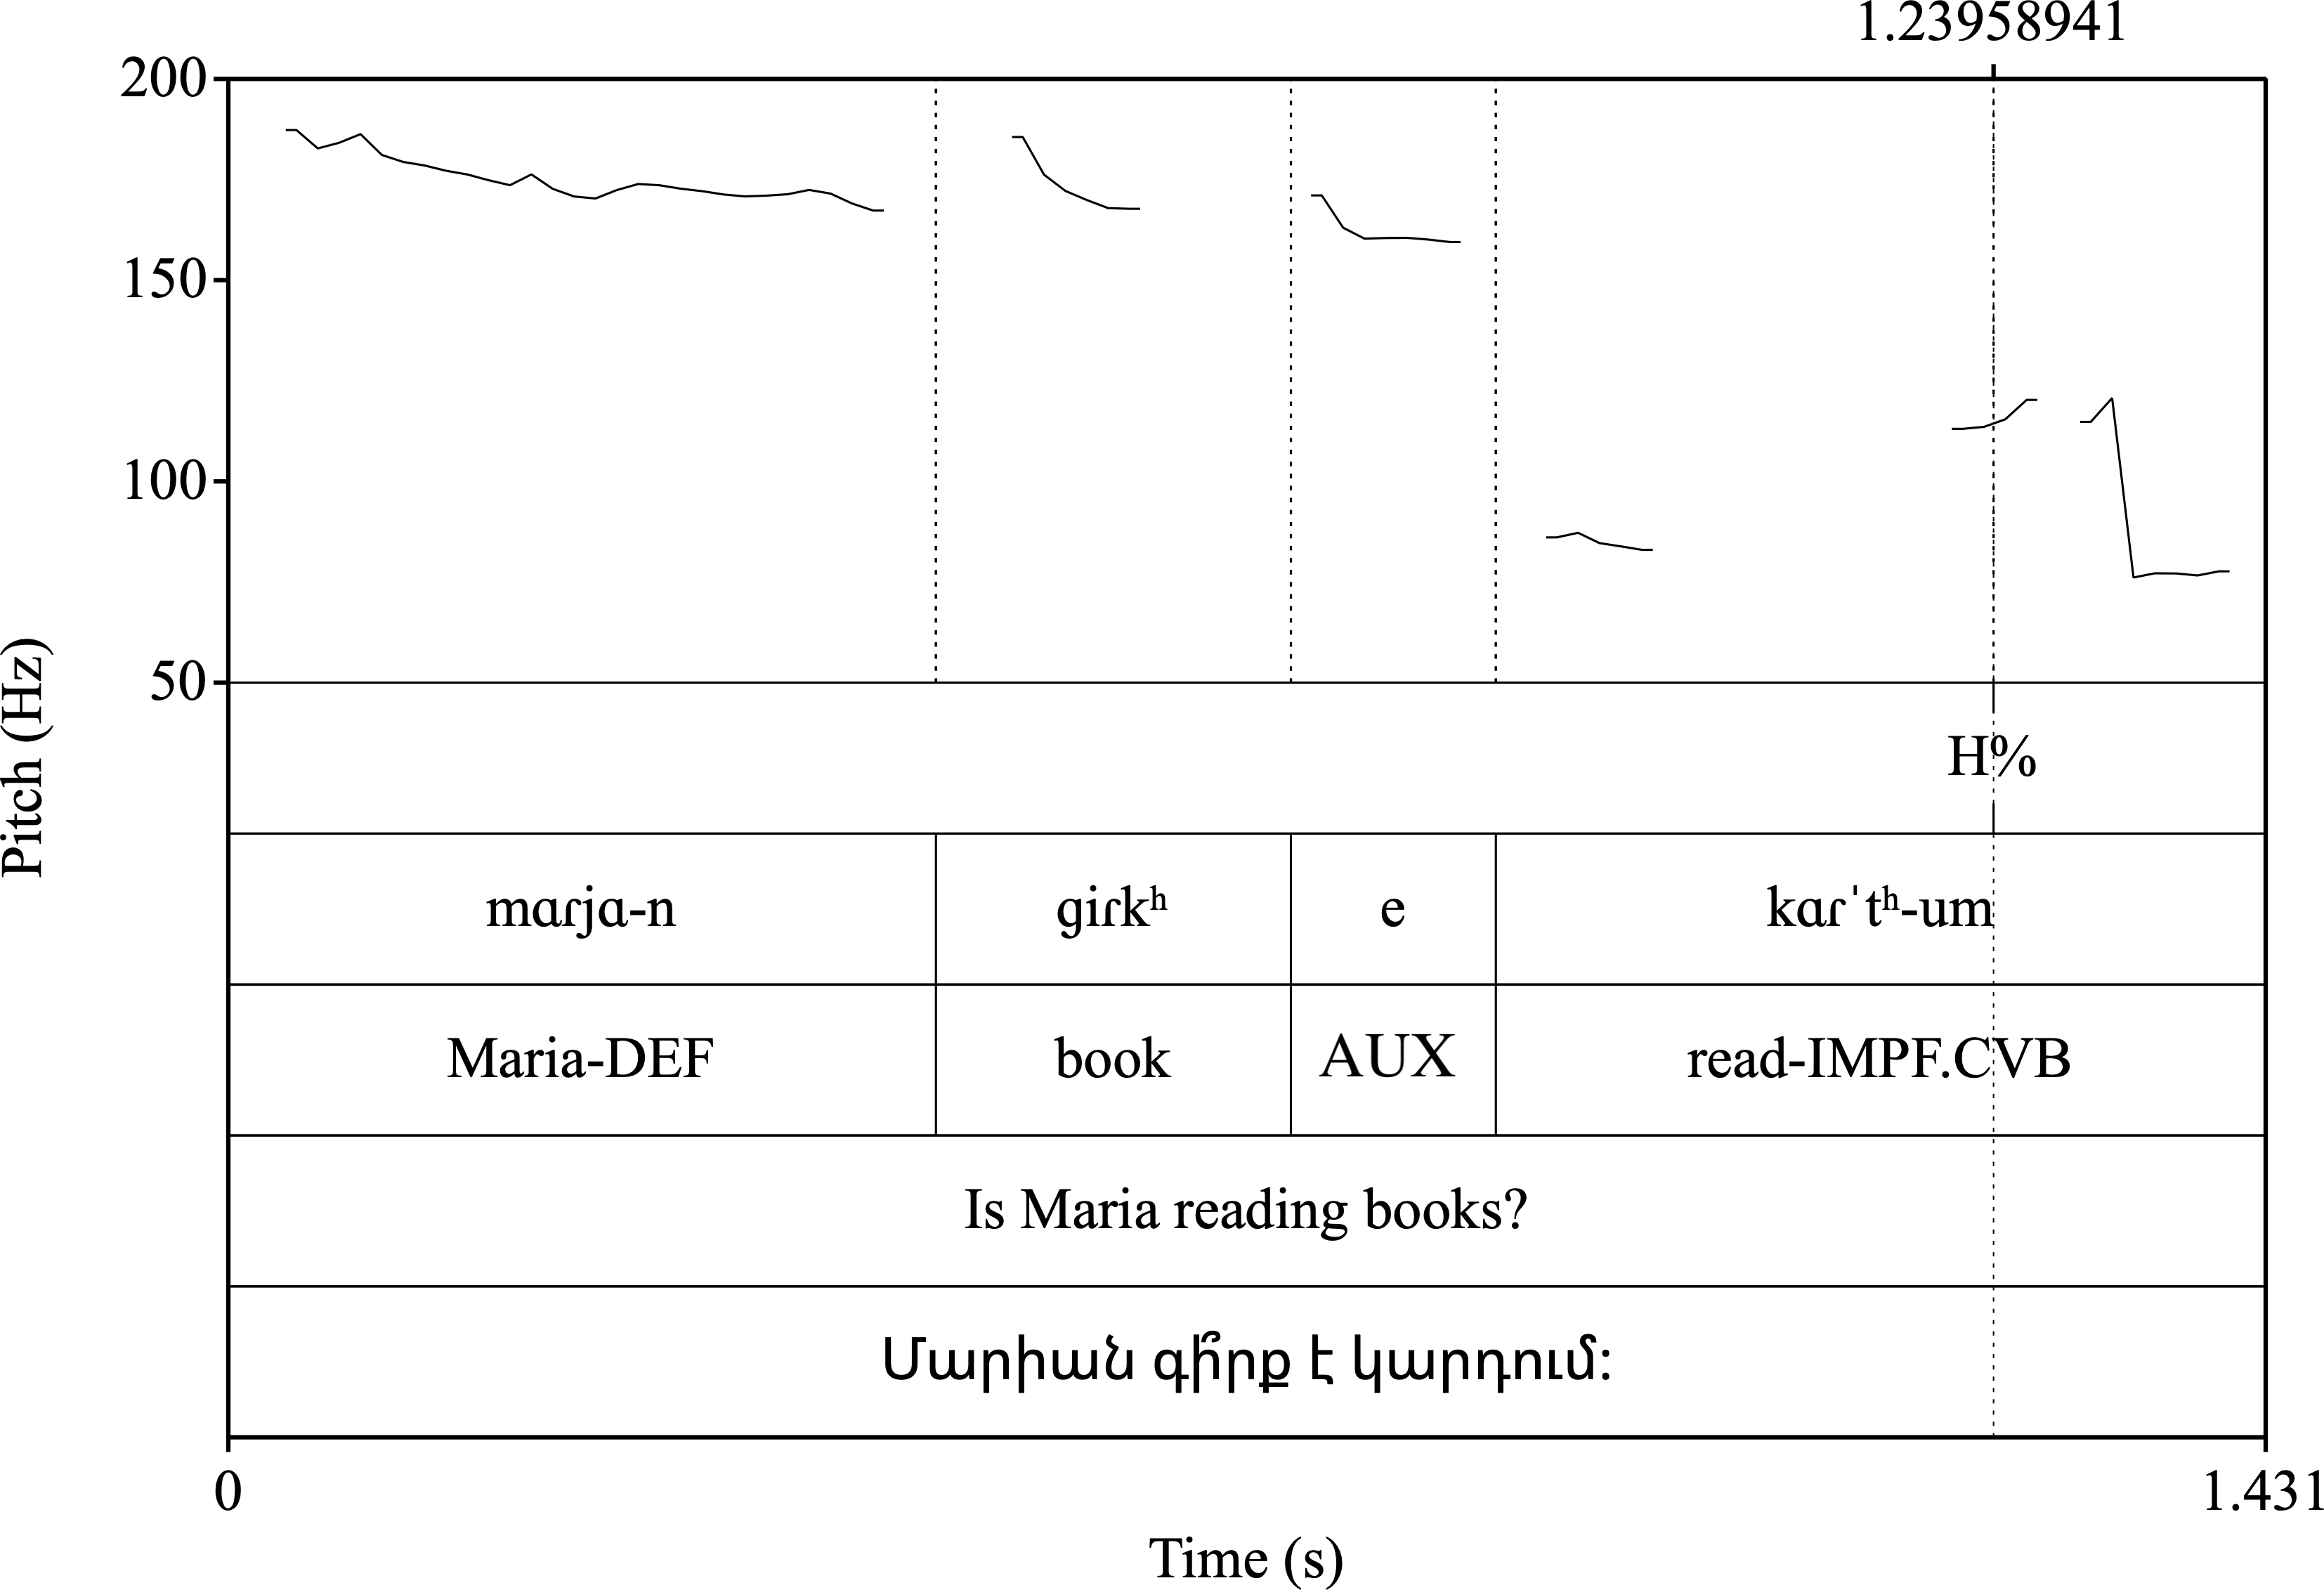
\includegraphics[scale= 0.6]{images/AT_PolarQuestion_HighTone.png}
		\end{figure}
		
		For {\iaIA}, the final syllable in a polar question can be considerably lengthened in order to indicate politeness. AS reports that final lengthening in {\iaIA} is common in order to indicate a non-aggressive and polite inquiry.
		
		Phonologically, the sentence-final H\% is on the final syllable of the polar question, regardless of whether that syllable carries lexical stress. 	For example, consider the following declarative sentence and its polar question form (\ref{example: v-aux dec sentence}). Morphologically, the sentence consists of a verb in a non-finite form, plus a   cliticized auxiliary. In the declarative, lexical stress and nuclear stress H* are on the last syllable of the verb, while the  clitic is unstressed and carries L\%. 
		
		
		\begin{exe}
			\ex 
			\begin{xlist}
				\ex \textit{Declarative    V-Aux with lexical stress on the V}\label{example: v-aux dec sentence}
				
				\begin{tabular}{l ll l}
					i.& {t͡sə\uline{χ-um}}  & ={e-s}$\searrow$&({\seaAbbre})
					\\
					ii.& {t͡sə\uline{χ-um}}  & ={e-s}$\searrow$&({\iaAbbre})
					\\
					& smoke-{\impfcvb} & {\auxgloss}-2{\sg} & \\
					&\multicolumn{3}{l}{`You smoke.'} 
					\\ 
					&\multicolumn{3}{l}{\armenian{Ծխում ես։}}
					\\
				\end{tabular} 
				\ex \textit{Polar question} \label{example: v-aux polar sentence}
				
				\begin{tabular}{llll}
					i.& {t͡sə\uline{χ-um}}$\nearrow$  & ={e-s}$\searrow$&({\seaAbbre})
					\\
					ii. &  {t͡səχ-um} &  ={e-s}$\nearrow$ &   ({\iaAbbre})
					\\
					& smoke-{\impfcvb} & {\auxgloss}-2{\sg} & \\
					& \multicolumn{3}{l}{`Do you smoke?'}
					\\
					&\multicolumn{3}{l}{\armenian{Ծխու՞մ ես։}}
					
					
				\end{tabular} 
				
			\end{xlist}
			
		\end{exe}
		
		
		In the polar form, the {\seaSE} version simply makes the nuclear stress more prominent, while the clitic keeps its L\% tone. But in {\iaIA}, sentence-final H\% is placed on the clitic. The proximity of H\% and the verb causes the verb to lose its nuclear stress.  	We show a pitch track for these sentences  in Figure \ref{fig:smoke pitch} from NK and AT.
		
		\begin{figure}
			\caption{Pitch track of declarative (\ref{example: v-aux dec sentence}) and polar question (\ref{example: v-aux polar sentence})   in {\seaAbbre}   and  {\iaAbbre} }
			\label{fig:smoke pitch}
			\begin{subfigure}[b]{0.5\textwidth}
				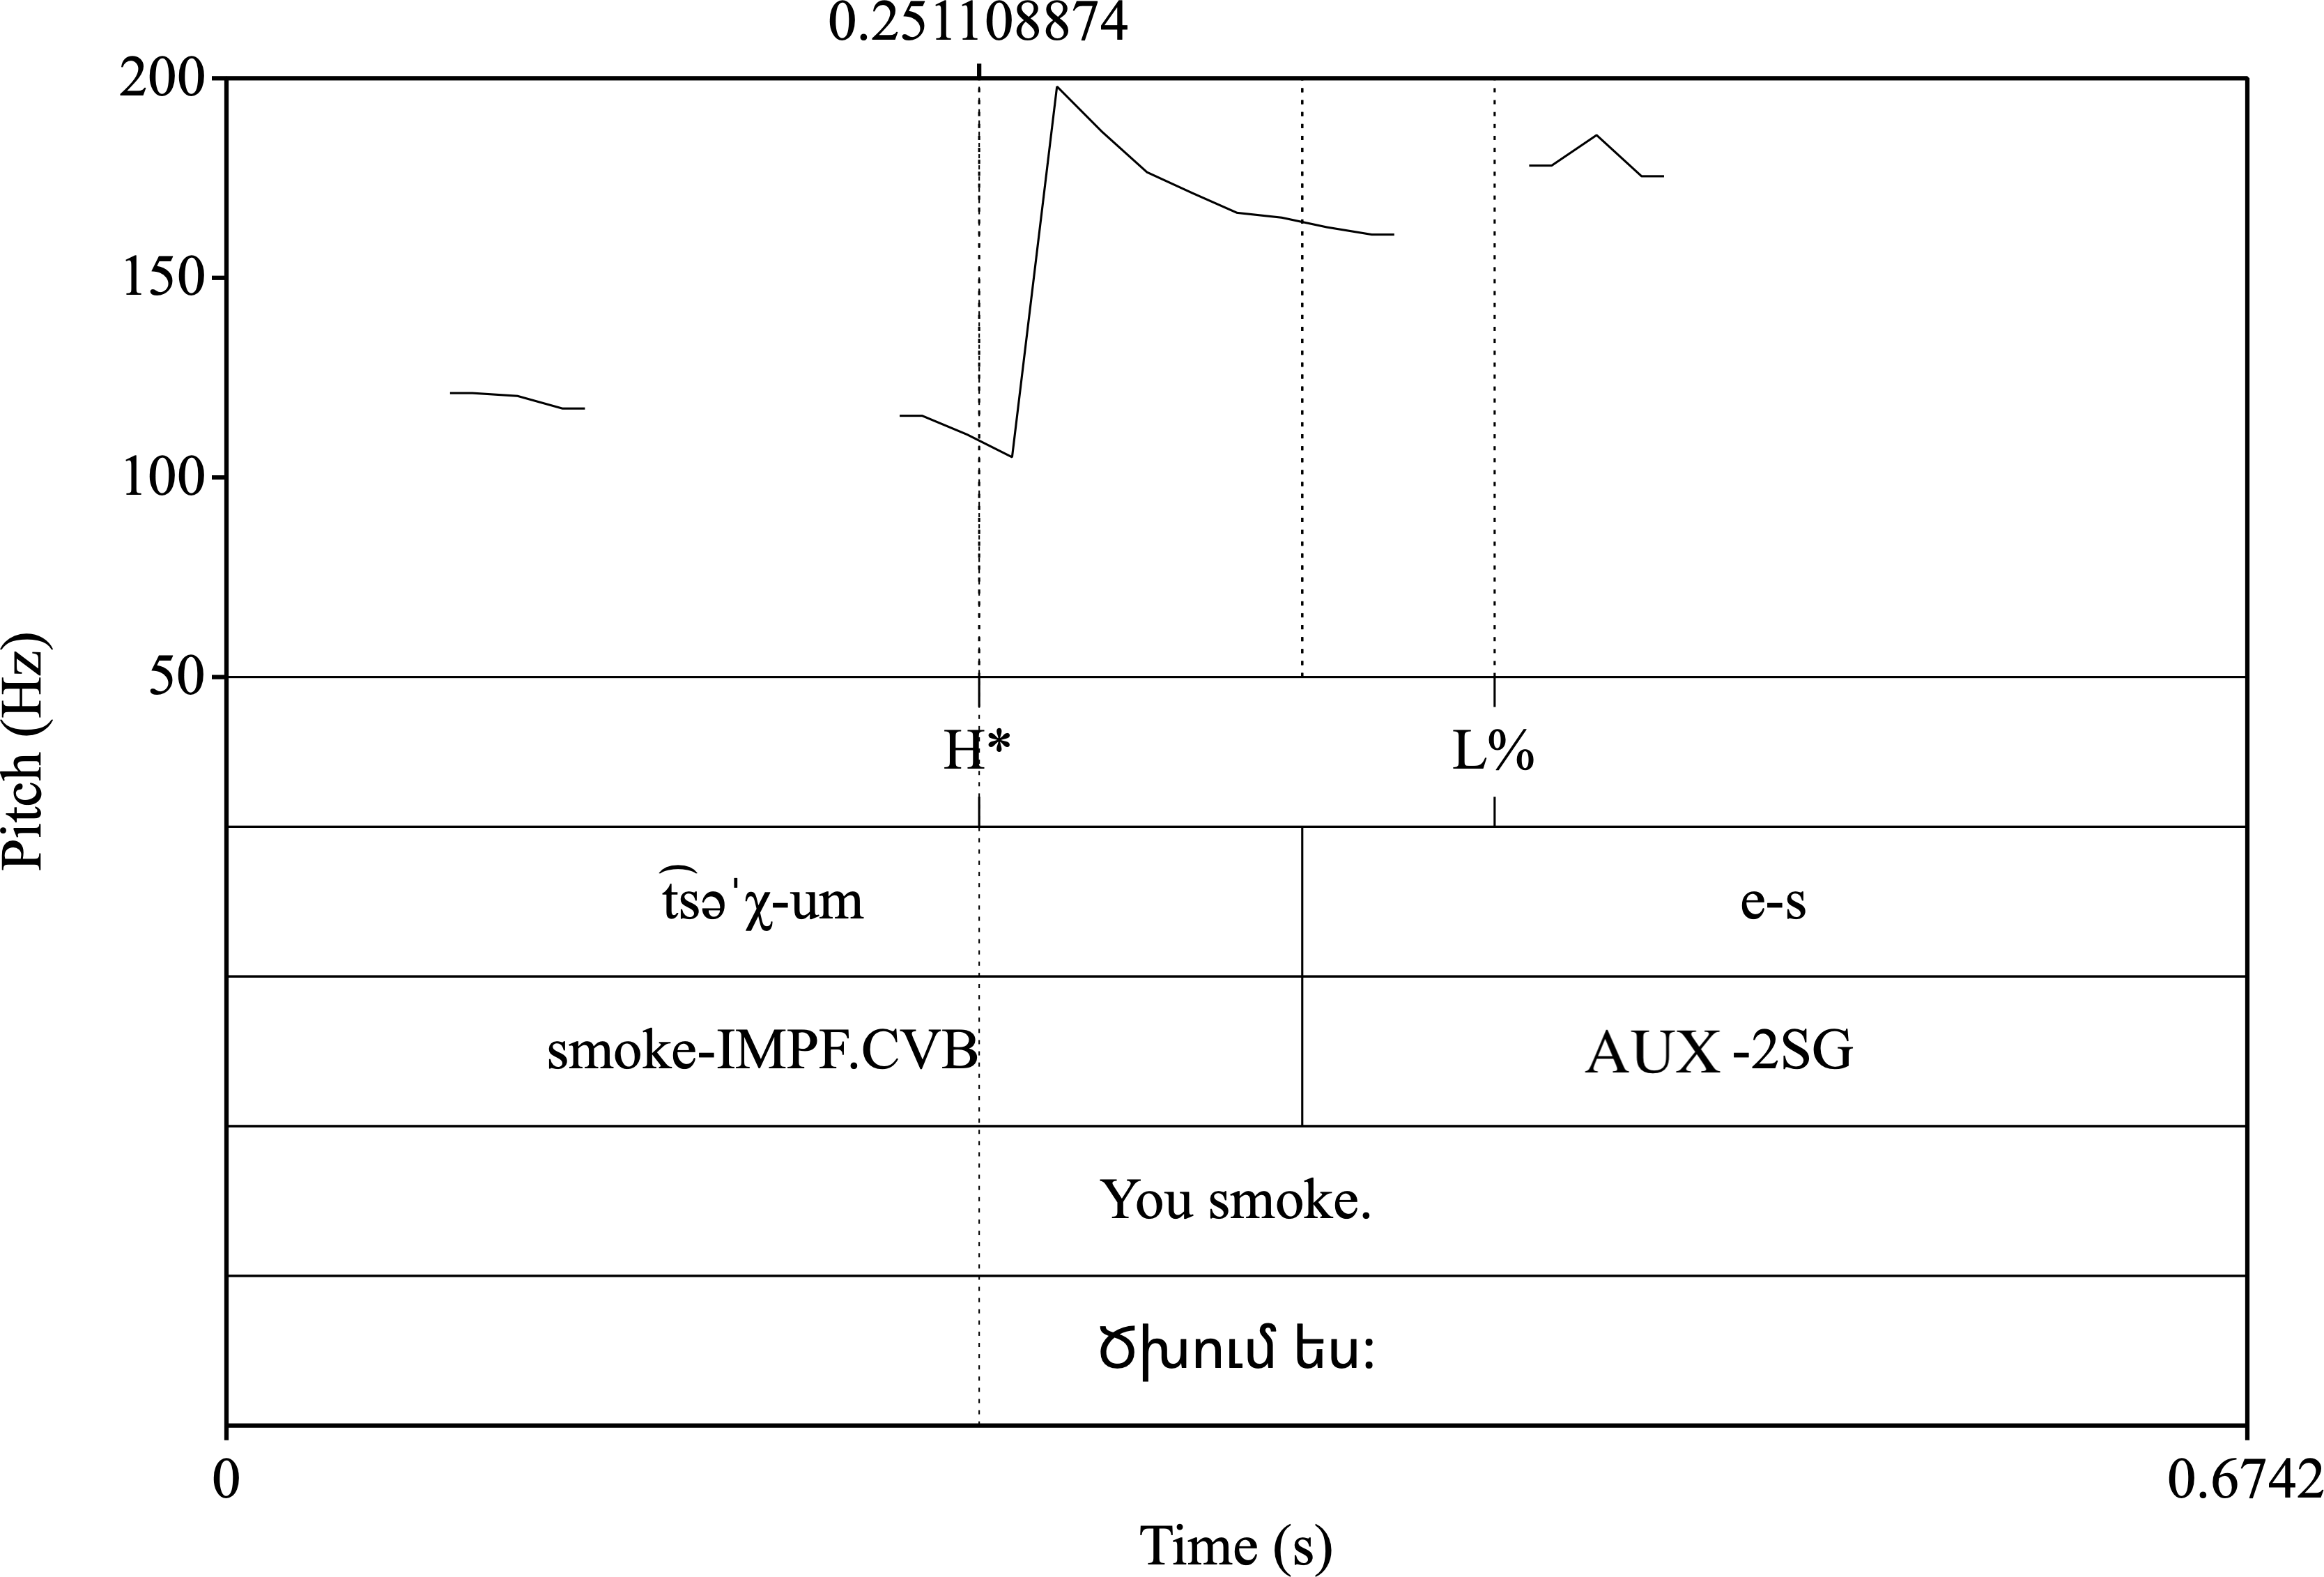
\includegraphics[width=\linewidth]{images/AT_Declarative_Clitic.png}
				\caption{{\seaAbbre} declarative   with L\%}
			\end{subfigure}%
			\begin{subfigure}[b]{0.5\textwidth}
				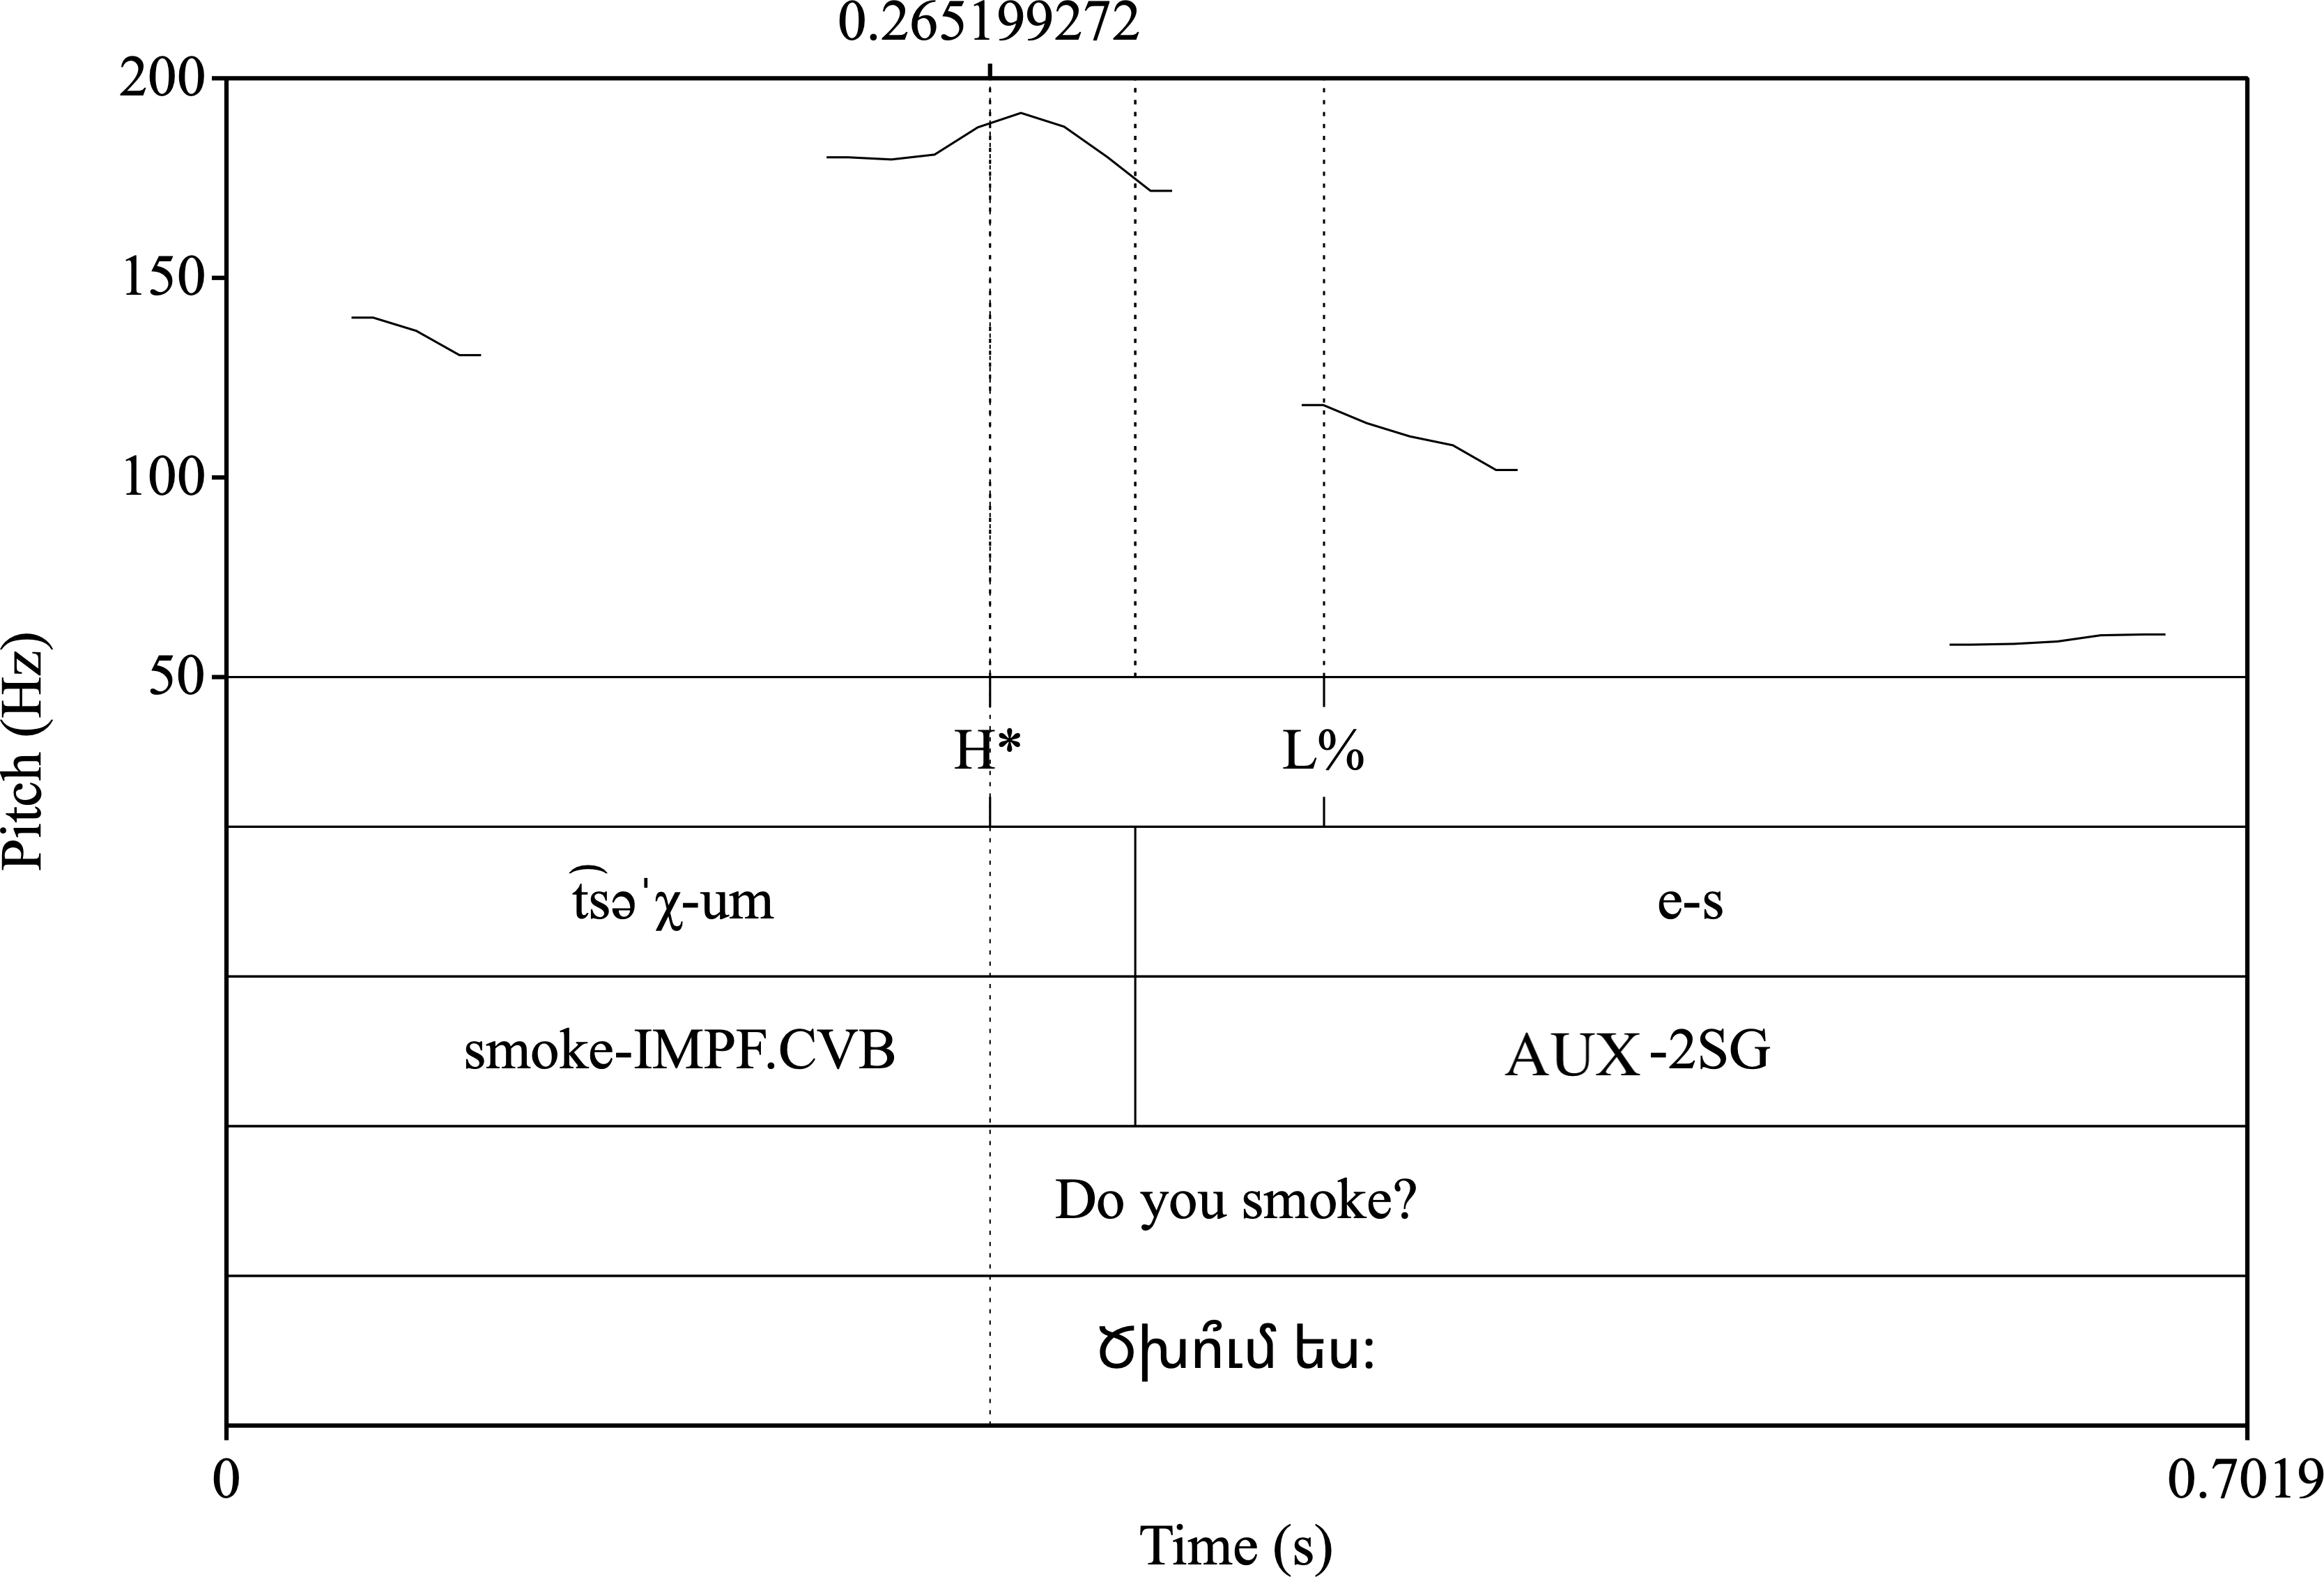
\includegraphics[width=\linewidth]{images/AT_PolarQuestion_Clitic.png}
				\caption{{\seaAbbre} polar  with L\%}
			\end{subfigure}\smallskip\\
			\begin{subfigure}[b]{0.5\textwidth}
				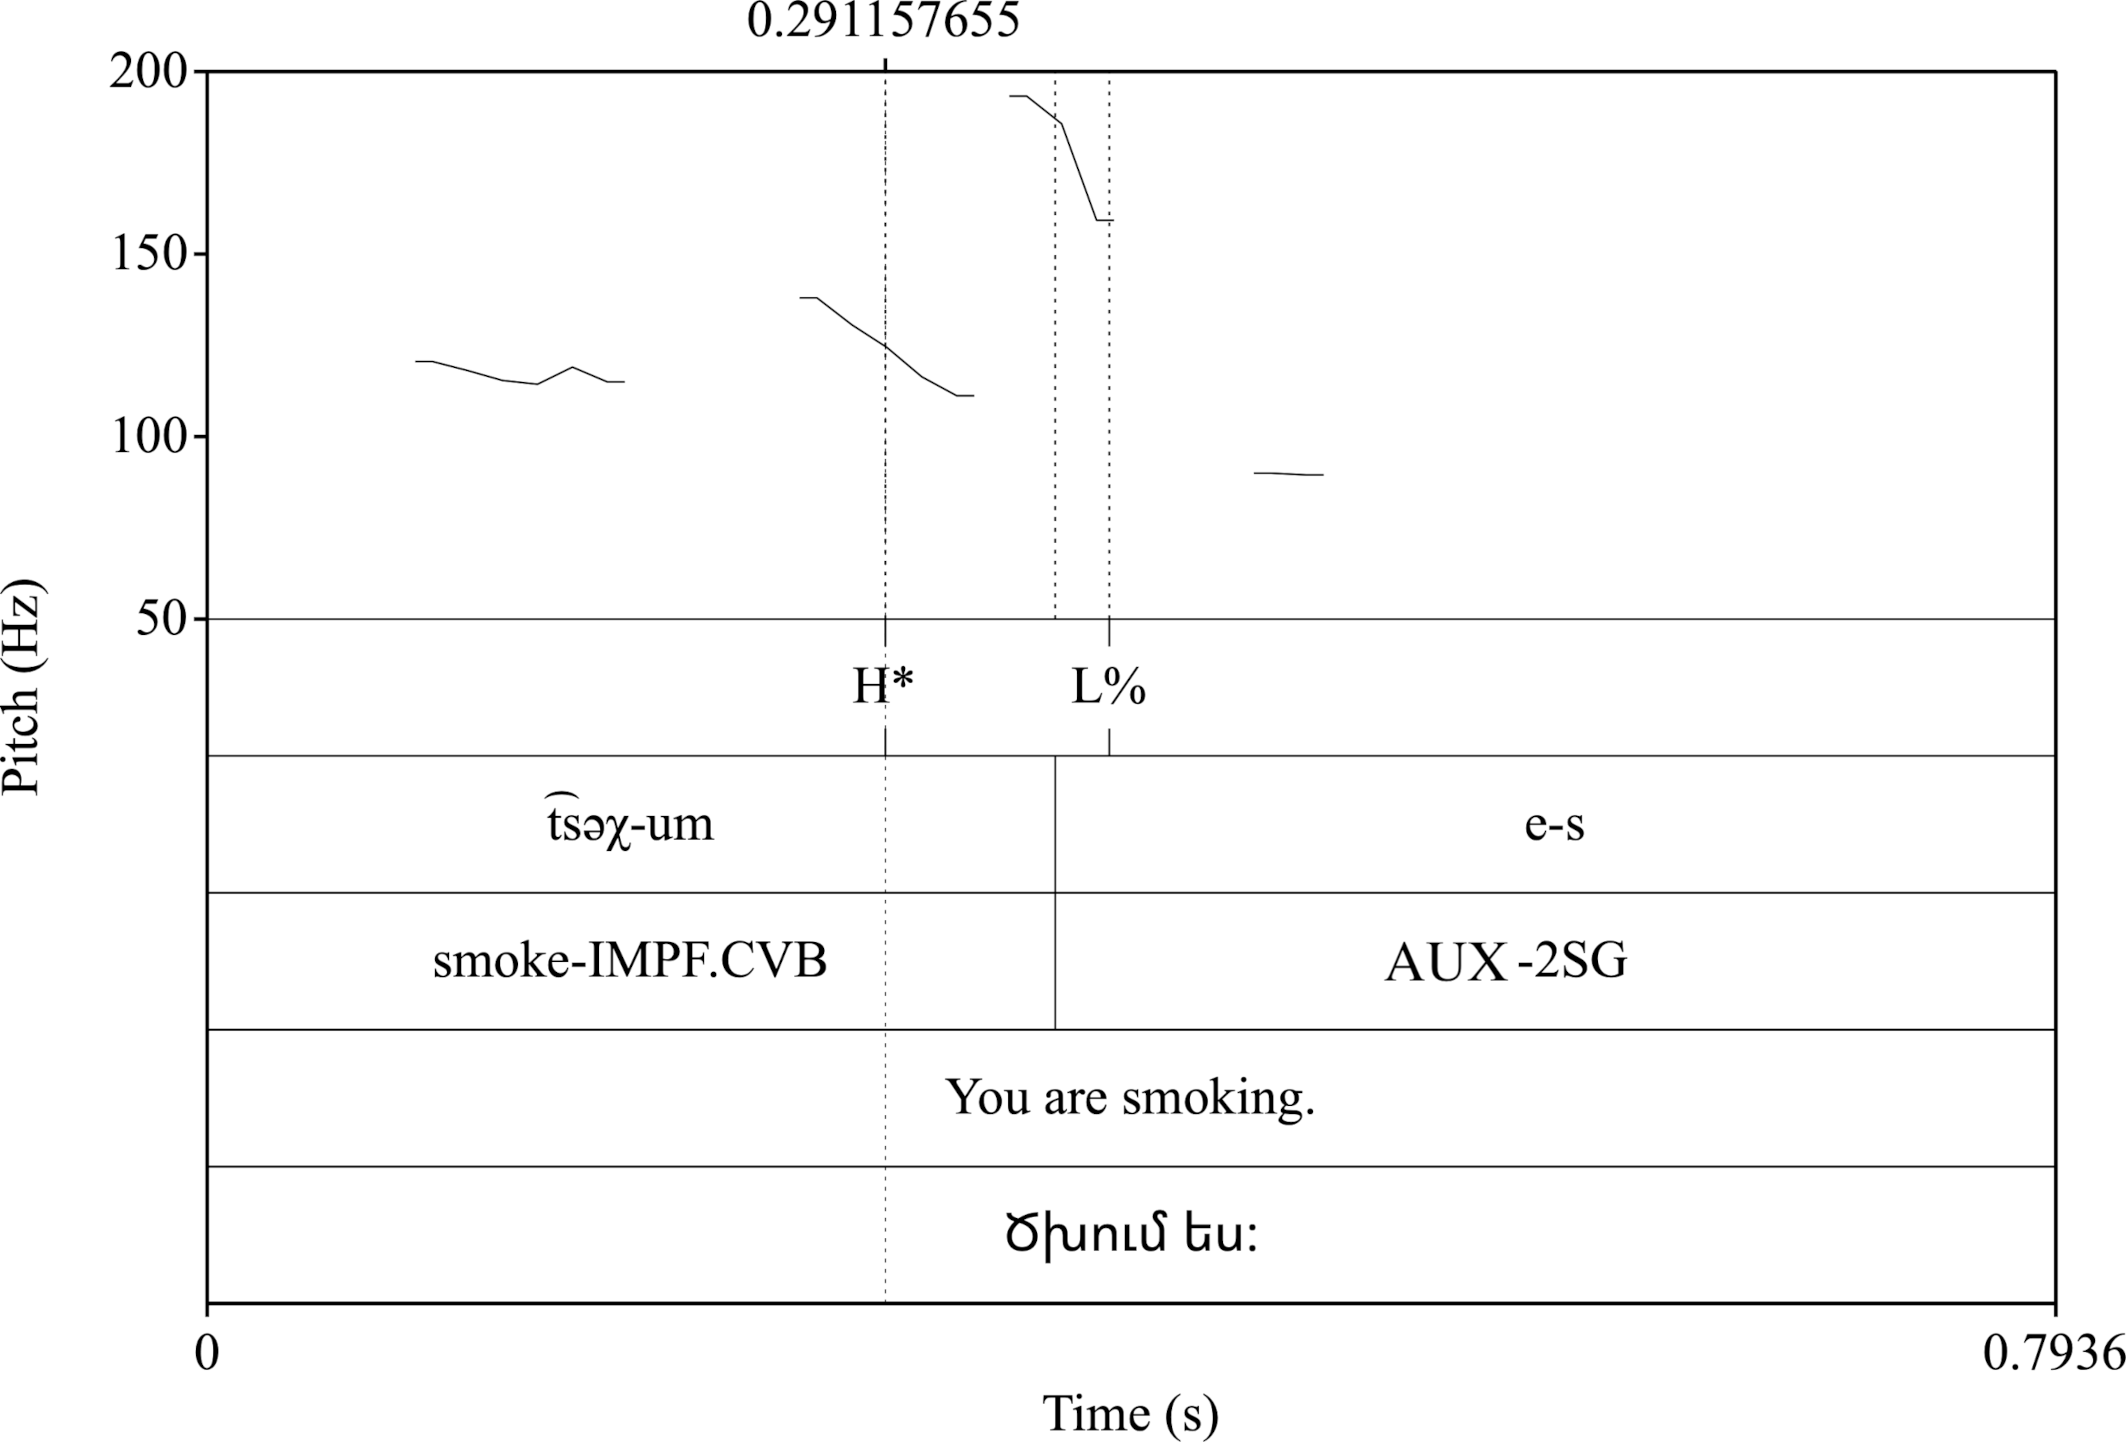
\includegraphics[width=\linewidth]{images/NK_Declarative_Clitic.png}
				\caption{{\iaAbbre} declarative   with L\%}
			\end{subfigure}%
			\begin{subfigure}[b]{0.5\textwidth}
				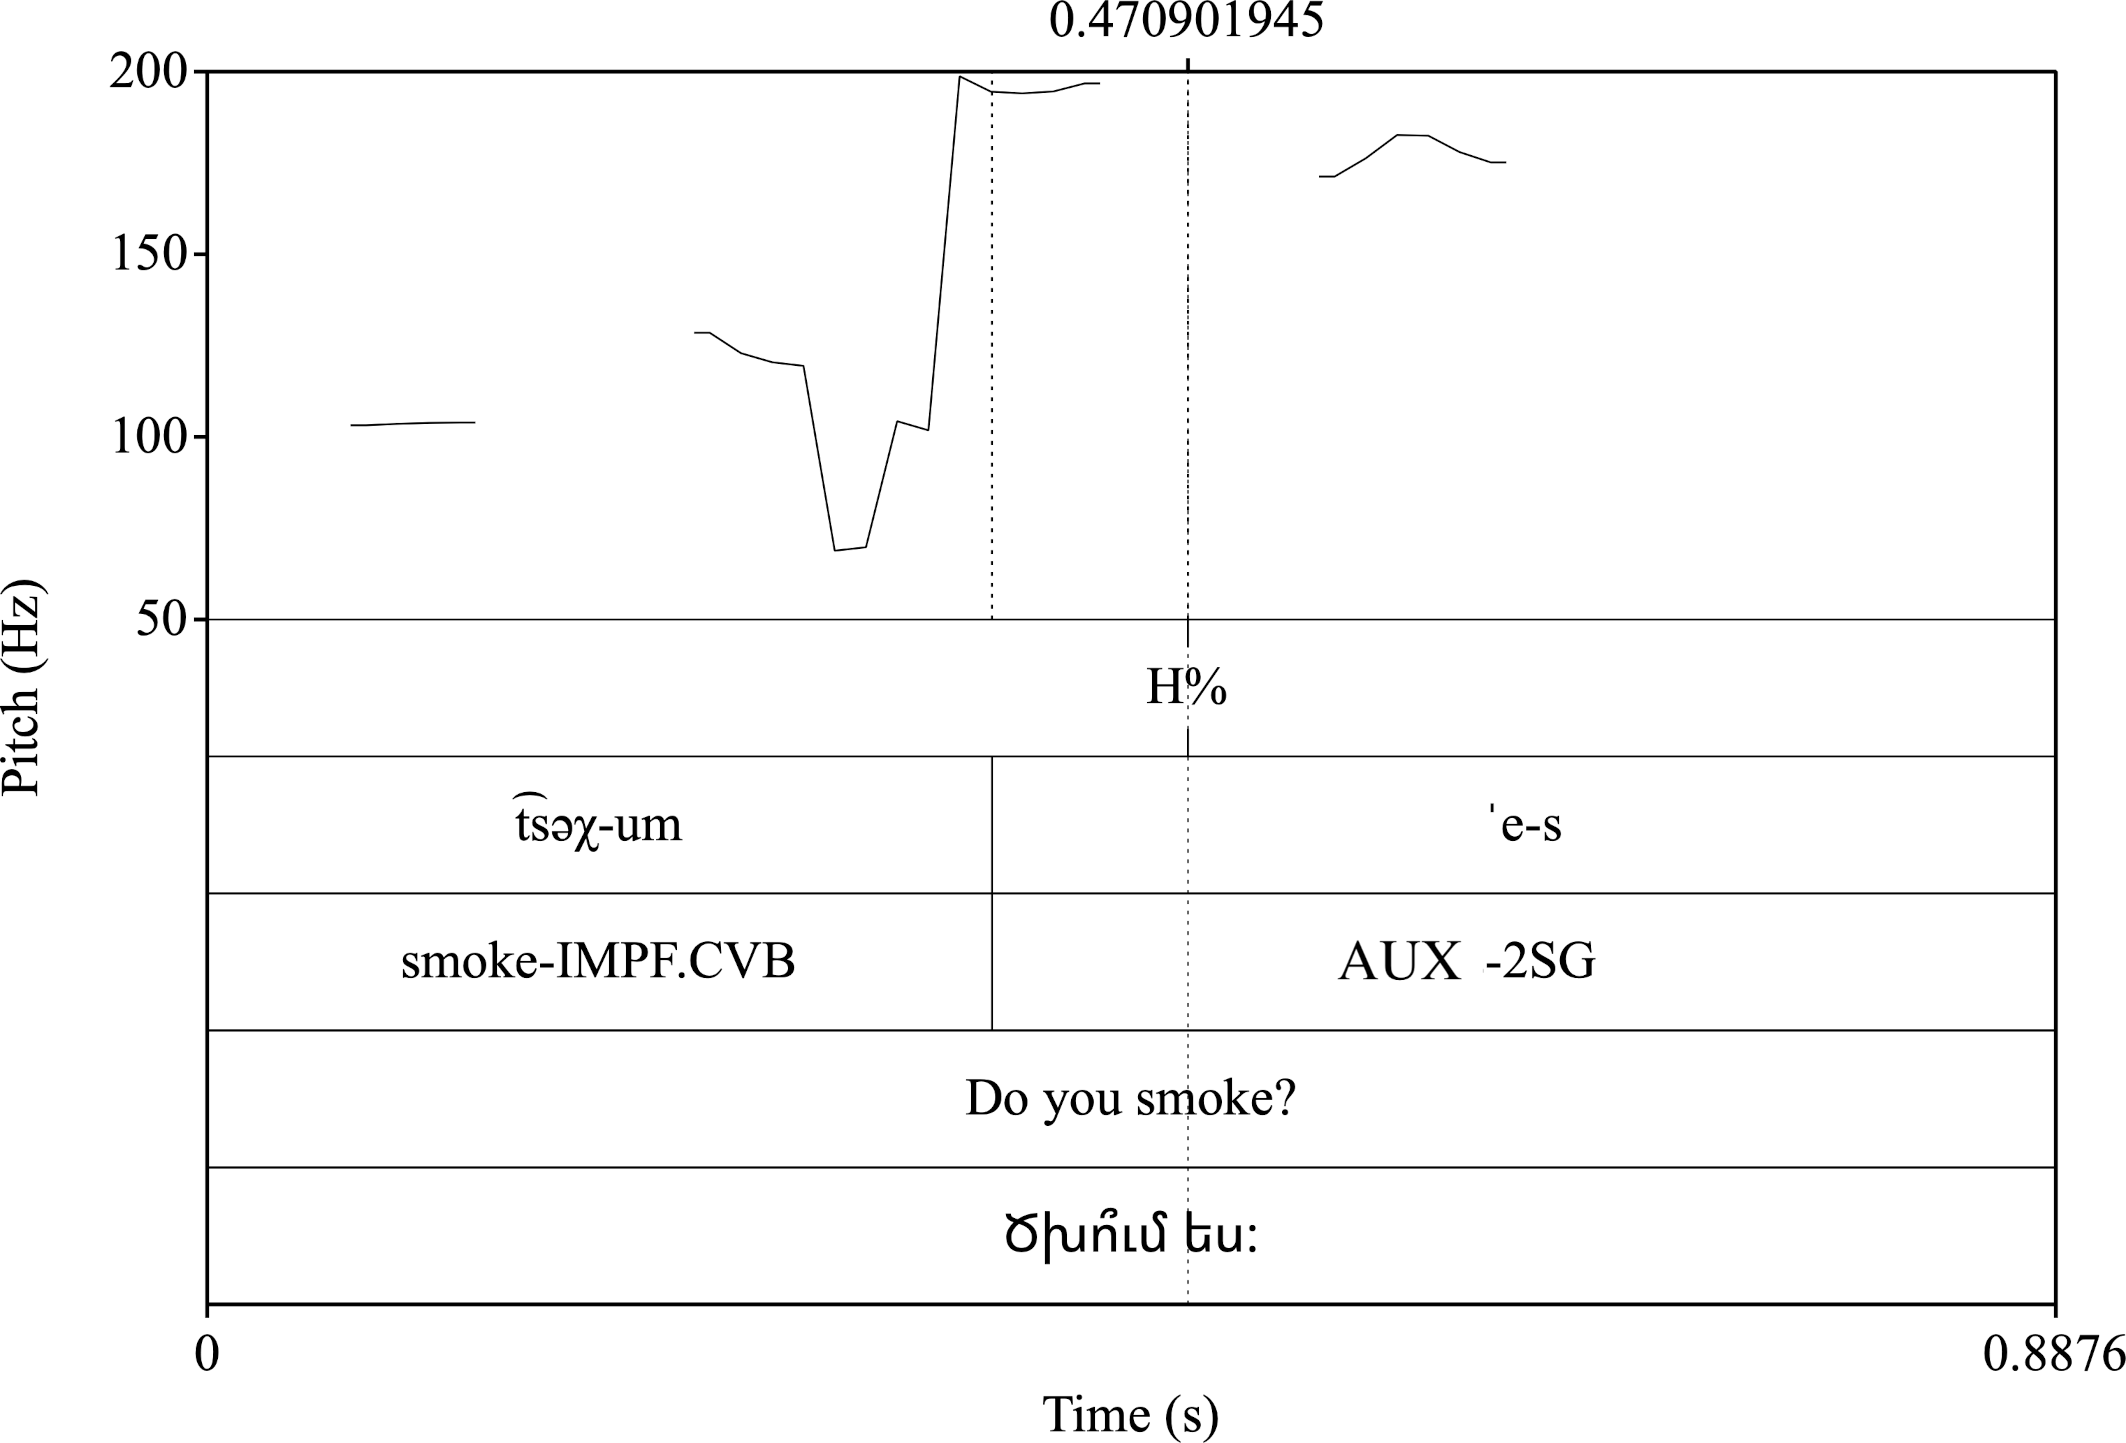
\includegraphics[width=\linewidth]{images/NK_PolarQuestion_Clitic.png}
				\caption{{\iaAbbre} polar  with H\%}
			\end{subfigure}
		\end{figure}
		
		
		
		Such lengthening and rising are also found in wh-questions (\ref{example: wh sentence}). In a subject wh-question in the present tense, the subject is replaced by the wh-word, takes nuclear stress, and is cliticized with the inflected auxiliary. There is a significant rise on the wh-word. The sentence ends with a falling intonation in  {\seaSE} \citep[15]{Johnson-1954-EastArmGrammar}. For {\iaIA}, the sentence can end  in a falling intonation in casual speech.   However, speakers can also  apply a sentence-final rise in order to indicate a degree of politeness.
		

		
		\begin{exe}
			\ex \textit{Subject wh-question}\label{example: wh sentence}
			
			\begin{tabular}{llllll}
				a.& {\uline{ov}}$\nearrow$&={e}& {{ɡiɾkʰ}}& {kɑɾtʰ-um}$\searrow$&({\seaAbbre})
				\\
				& \multicolumn{5}{l }{\armenian{Ո՞վ է գիրք կարդում։}}\\
				b. & {\uline{ov}}$\nearrow$&={ɒ}&   {{ɡiɻkʰ}} & {kɒɻtʰ-um}$\searrow$&({\iaAbbre} - Casual)
				\\
				c. & {\uline{ov}}$\nearrow$&={ɒ}&   {{ɡiɻkʰ}} & {kɒɻtʰ-um}$\nearrow$&({\iaAbbre} - Polite)
				\\
				& who&={\auxgloss}&book& read-{\impfcvb} & 
				\\
				&\multicolumn{4}{l}{`Who is   reading  books?'
				} & 
				\\
				& \multicolumn{5}{l }{\armenian{Ո՞վ  ա գիրք կարդում։}} \\
				
			\end{tabular} 
			
		\end{exe}
		
		Figure \ref{fig:wh iranian low high} (page \pageref{fig:wh iranian low high}) shows the recordings for the above wh-question, one with a final fall L\%, and one with a final rise H\%.  Data is from NK. She at first produced the falling sentence, but in subsequent elicitations preferred the rising sentence.\largerpage[-1]
		
		
		
		
		\begin{figure}
			\caption{Pitch track of wh-question from (\ref{example: wh sentence}) with a final fall (\ref{example: wh sentence}a,b) or with a final rise  (\ref{example: wh sentence}c)  in {\seaSE} and {\iaIA}\label{fig:wh iranian low high}}
			\begin{subfigure}[b]{0.5\textwidth}
				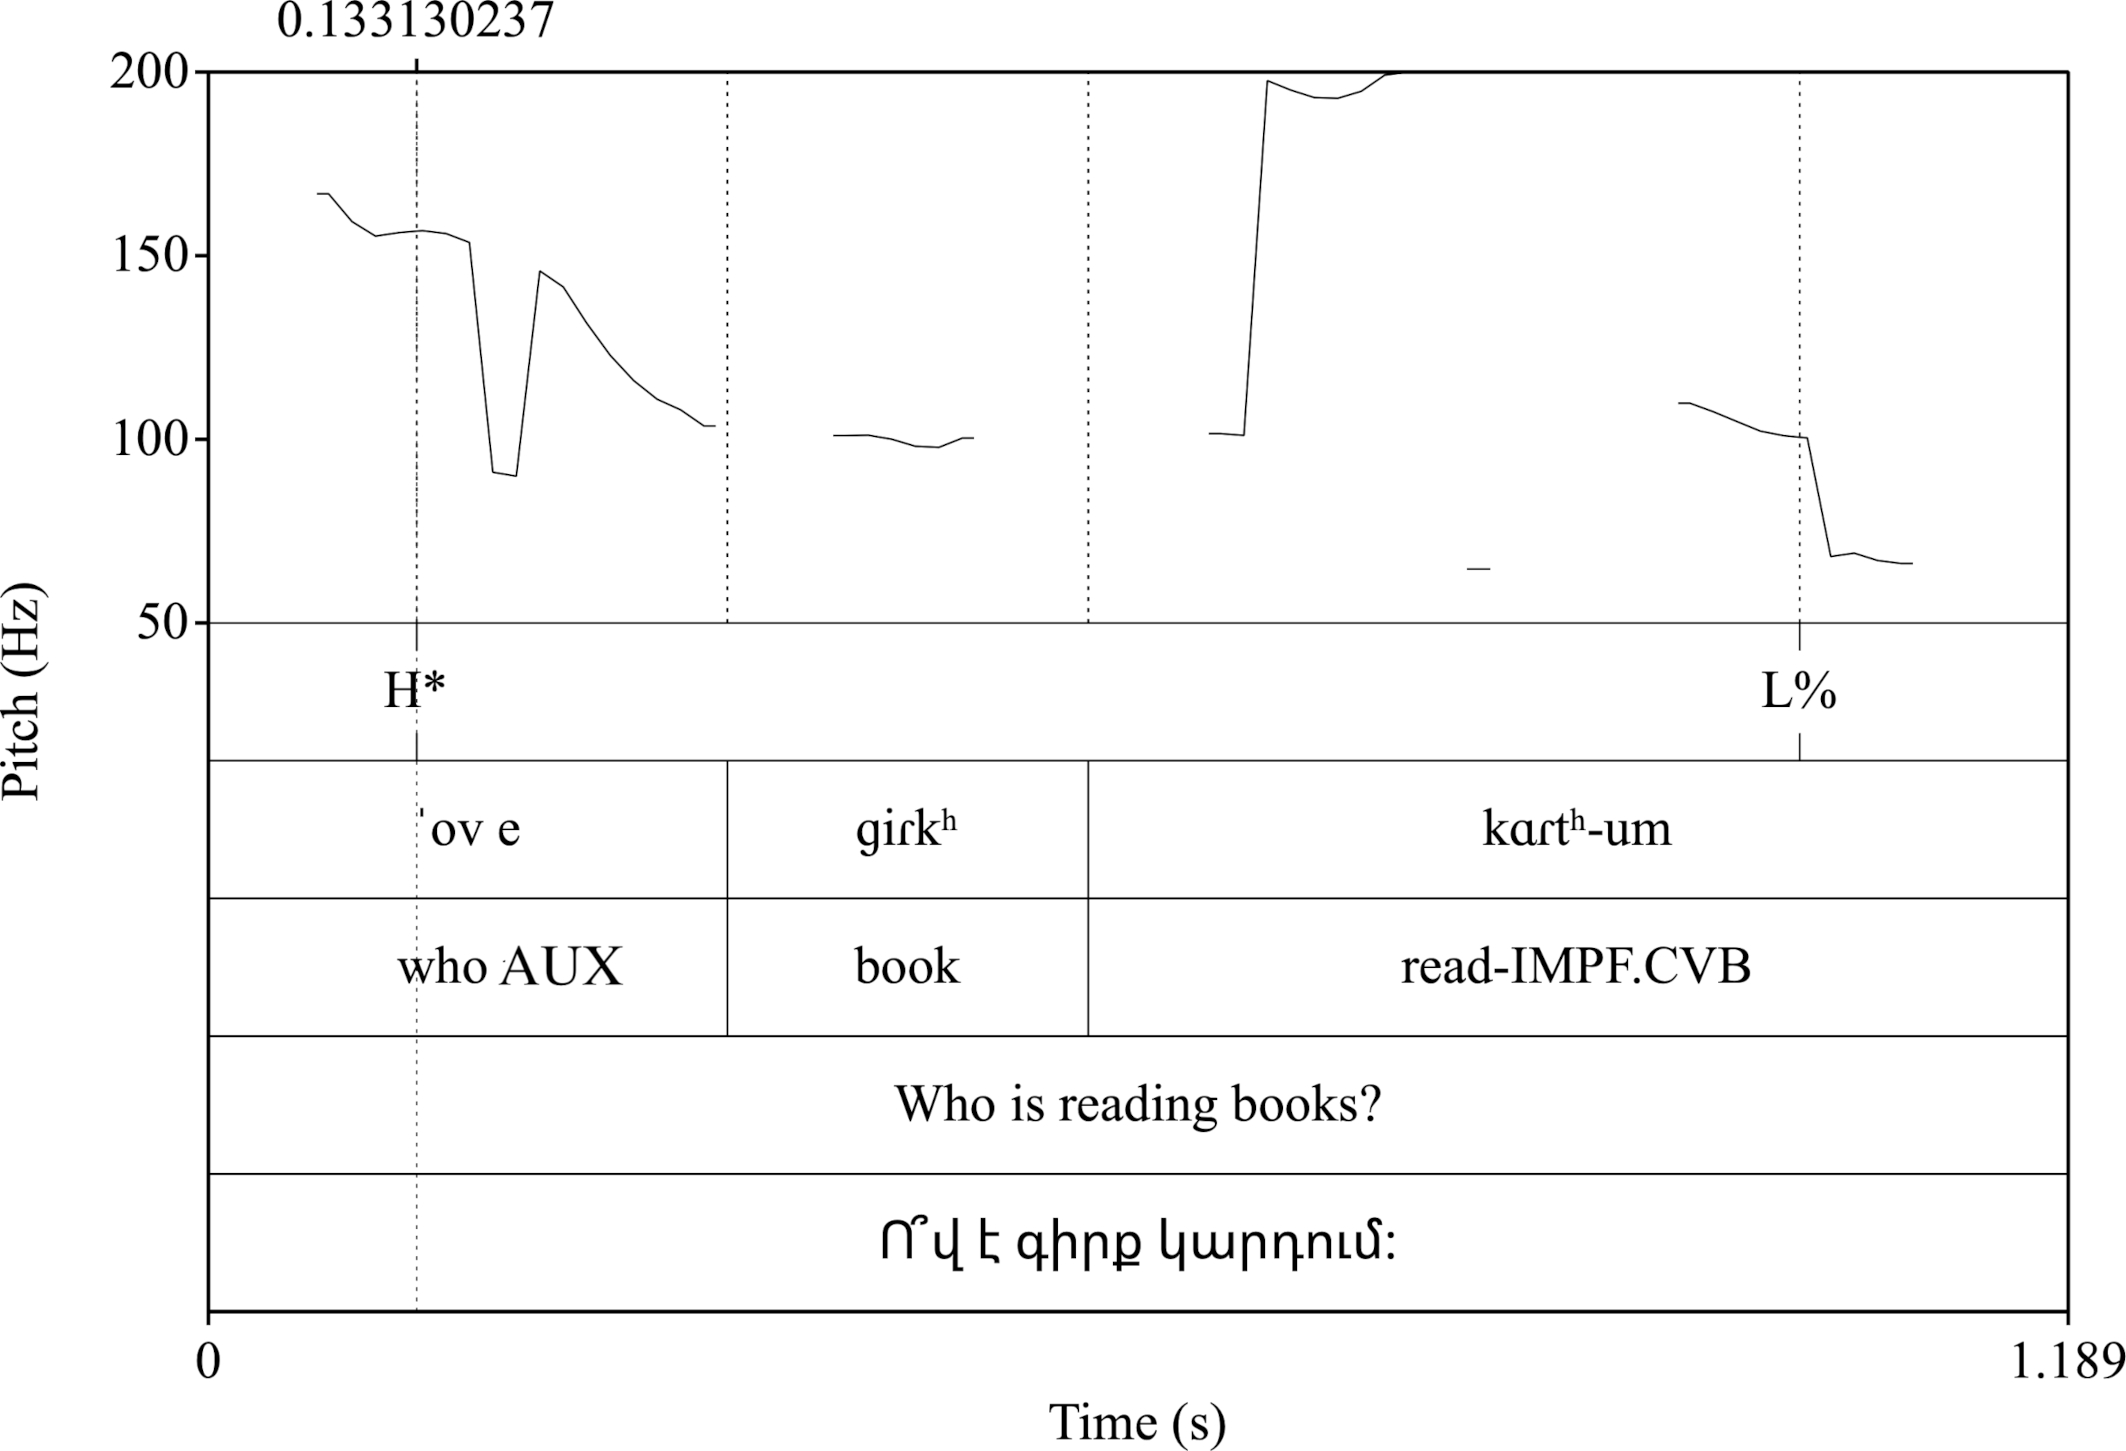
\includegraphics[width=\linewidth]{images/AT_WhQuestion.png}
				\caption{{\seaAbbre} wh-question with L\%}
			\end{subfigure}%
			\begin{subfigure}[b]{0.5\textwidth}
				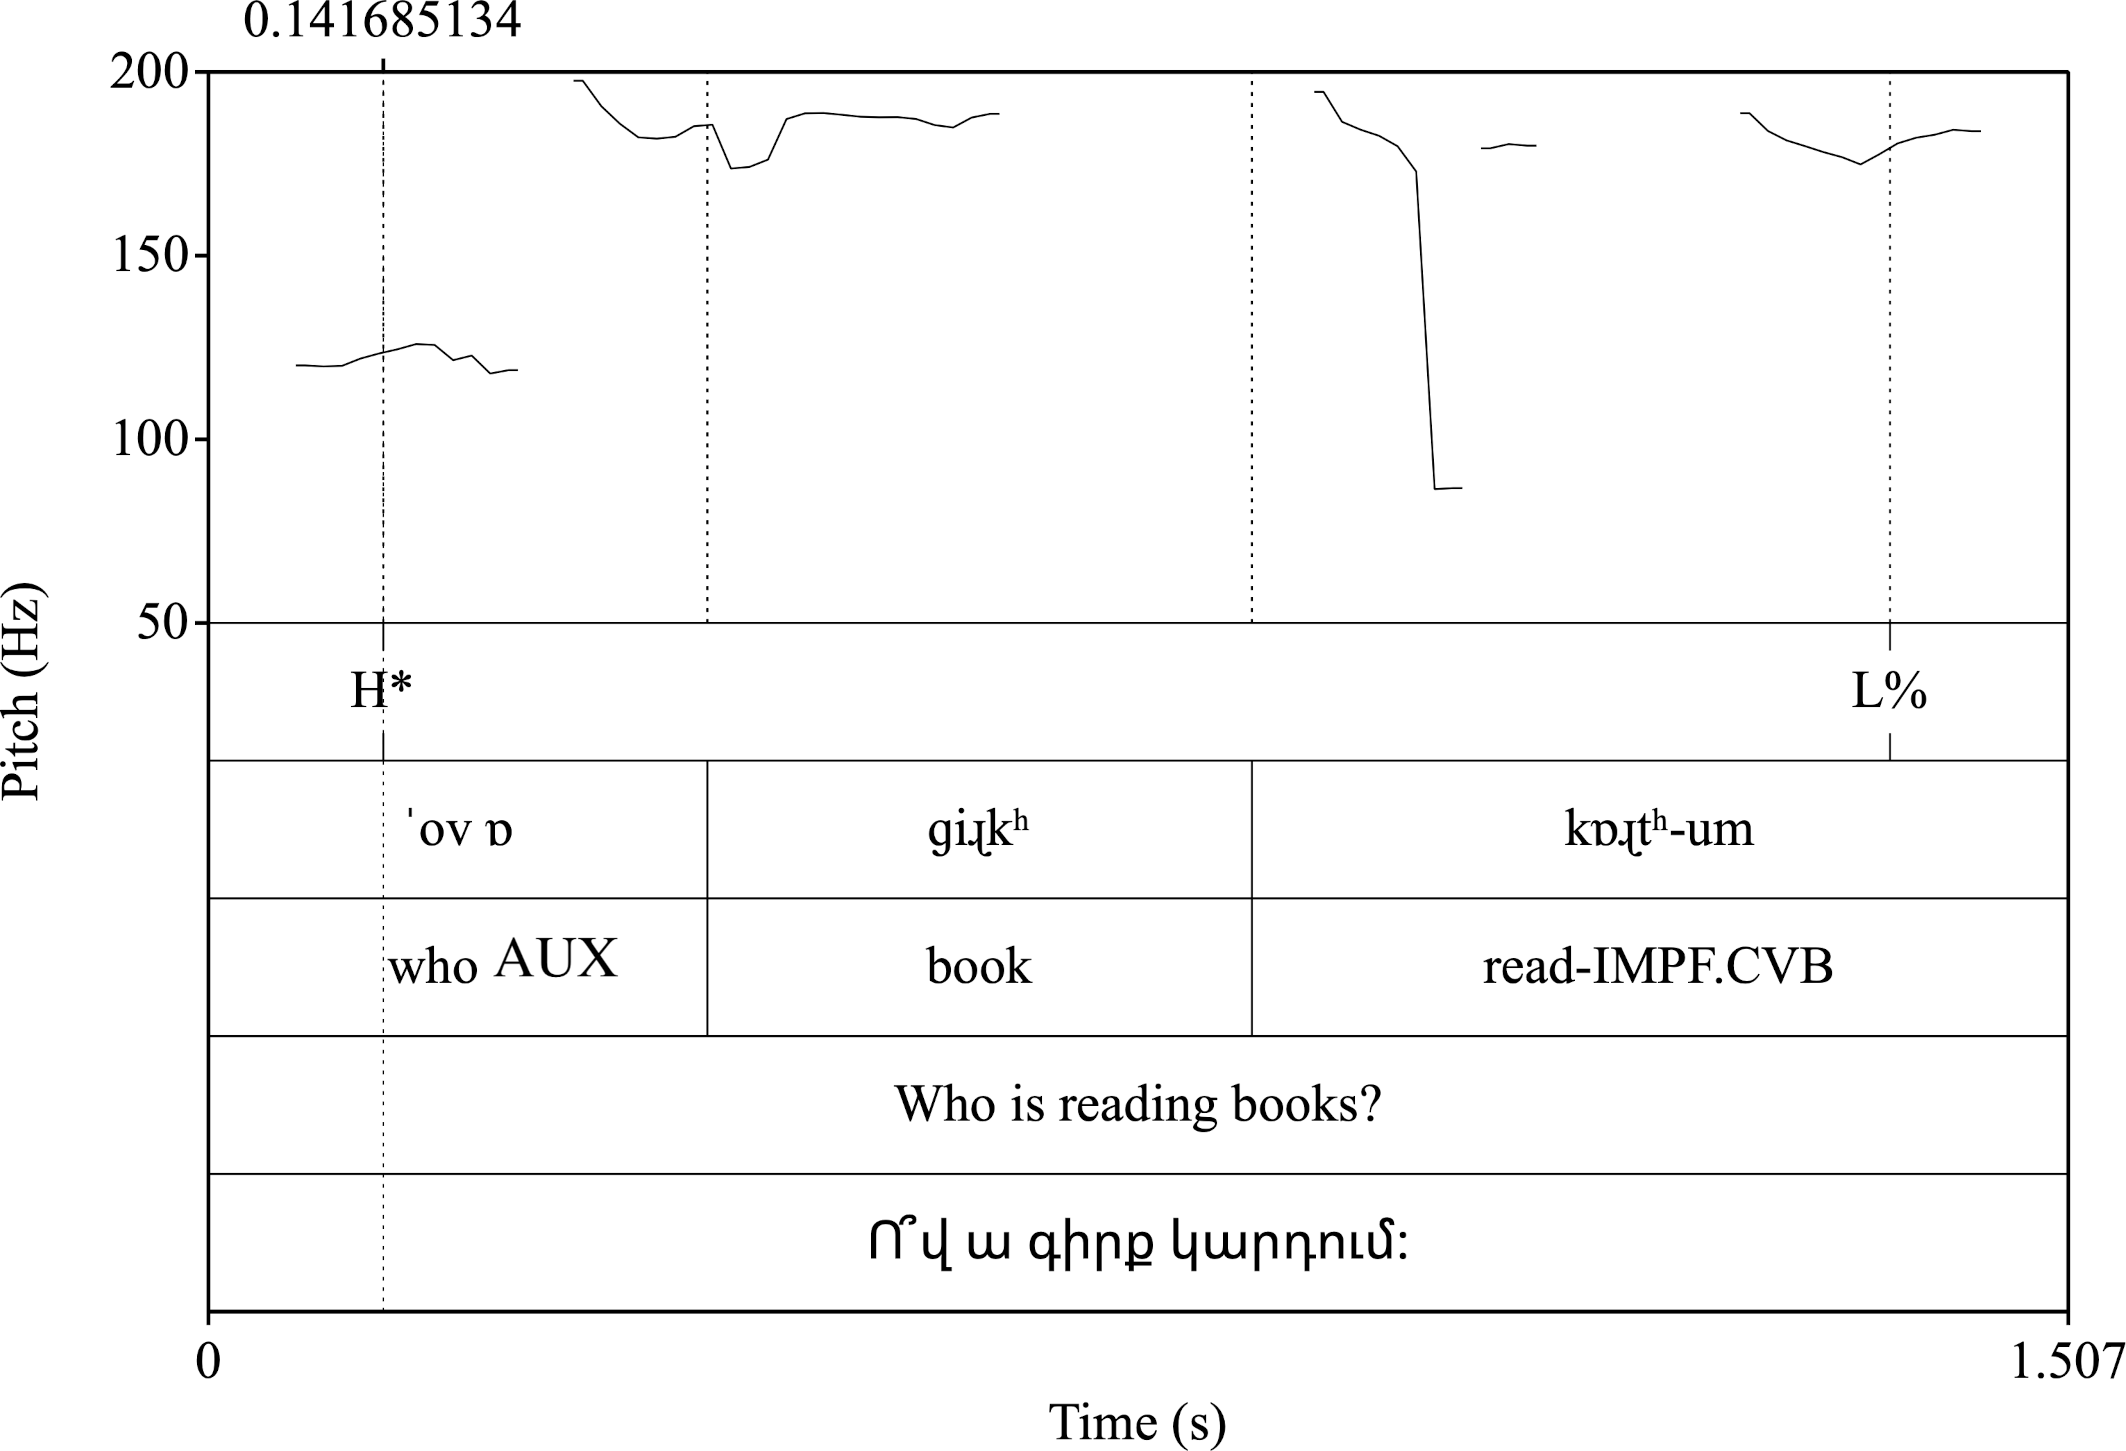
\includegraphics[width=\linewidth]{images/NK_WhQuestion_LowTone.png}
				\caption{{\iaAbbre} wh-question with L\%}
			\end{subfigure}\smallskip\\
			\begin{subfigure}[b]{0.5\textwidth}
				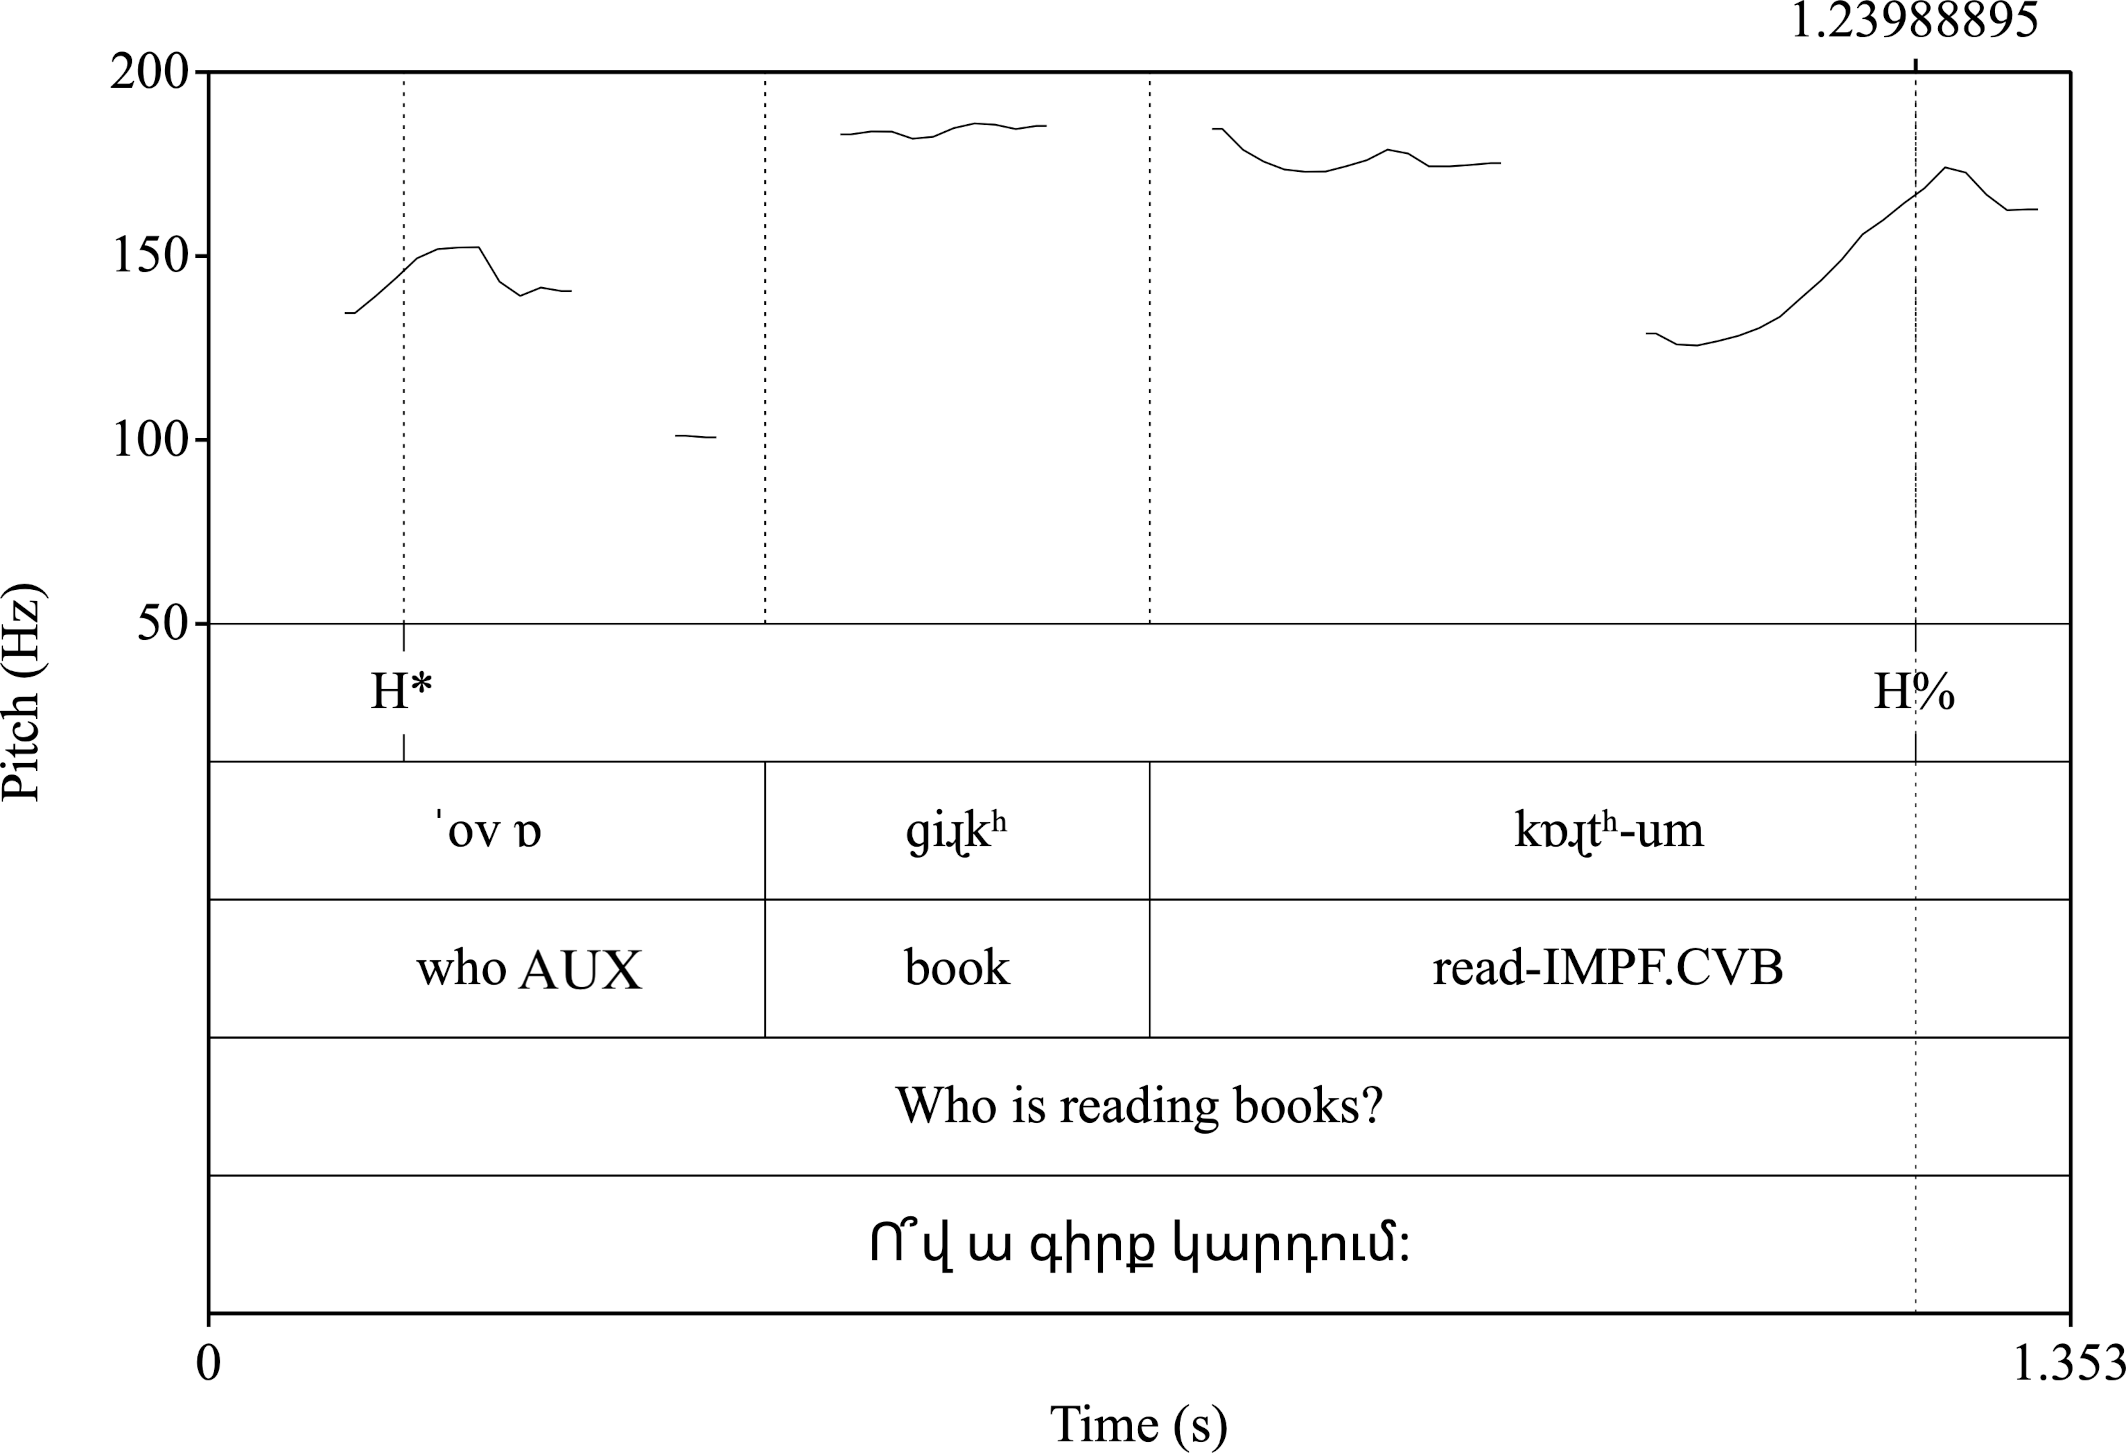
\includegraphics[width=\linewidth]{images/NK_WhQuestion_HighTone.png}
				\caption{{\iaAbbre} wh-question with H\%}
			\end{subfigure}			
		\end{figure}
		
		In Persian, wh-questions likewise end in falling intonation \citep[118]{sadat-2011-intonationPatternsInterrogativesPersian}. Such questions can undergo a final rise and lengthening in order to indicate politeness, curiosity, or a sense of not asserting the question (Sadat-Tehrani, p.c.).  The use of a final rise in wh-questions seems to have become somewhat conventionalized in {\iaIA}. For example, NK produced some wh-questions with     final rises, and some wh-questions with final falls. But she more often used final rises than final falls.   More data is however needed to establish the frequency of using sentence-final rises vs. falls in wh-questions across multiple speakers. 
		
		Finally, recall that {\seaSEA} is used by the Armenian community in Iran as a formal register. It is possible that a contributing factor to the intonational difference between {\seaSE} and {\iaIA} is the fact that Persian utilizes lower pitch in formal contexts \citep{falahati-2020-acquisitionSegmentalSuprasegmentalFeaturesSecondLanguagePersianPoliteness}. Thus, {\iaIA} might have conventionalized the use of sentence-final rises in order to further reinforce the sociolinguistic distinction between formal {\seaSE} and informal {\iaIA}.  
		
		
		In sum, {\iaIA} has adopted aspects of Persian intonation. Such aspects are not due to code switching. It seems that in general, {\iaIA} speakers born in the diaspora (like NK)   do not acquire Persian at the home. 

\chapter{Morphophonology}\label{section:morphophono}

In terms of the interaction between morphology and phonology, we discuss mor\-phol\-o\-gi\-cal\-ly-in\-duced phonological processes (\S\ref{section:morphophono:morphophono}),  phonologically-con\-di\-tioned allomorphy (\S\ref{section:morphophono:allomorphy}), and a phonosyntactic process that references both phonology and syntax (\S\ref{section:morphophono:auxiliary}). 

\section{Morphophonological alternations}\label{section:morphophono:morphophono}
Besides general phonology, Armenian dialects show various morphophonological rules which operate at morpheme boundaries. This includes root-initial glide insertion (\S\ref{section:morphophono:morphophono:root initial glide}), vowel hiatus repair under suffixation/cliticization (\S\ref{section:morphophono:morphophono:vowel hiatus}), and high vowel   reduction under suffixation (\S\ref{section:morphophono:morphophono:vowel reduction}).  

In general,   morphophonological processes that are attested in {\seaSEA}  are also attested in {\iaIA}. But in the judgments of KM, ``phonological changes at morpheme boundaries are becoming simpler in {\iaIA}.'' This ``simplicity'' suggests that such processes apply less often in {\iaIA} than in {\seaSEA}. For an overview of such morphophonological processes in {\seaSE} and {\swaWA}, see \citet[\S1]{Vaux-1998-ArmenianPhono} and \citet[\S2]{Dolatian-2020-Diss}.


\subsection{Root-initial glide insertion }\label{section:morphophono:morphophono:root initial glide}
Armenian is primarily suffixing, and there are few morphophonological rules that are sensitive to prefix boundaries. The most noticeable process is root-initial  “diphthongization” or glide insertion.

The Classical Armenian grapheme \armenian{ե} 
was a mid vowel \textit{{e}} \citep{Macak-2017-PhonoClassicalArmenian}. In the diachronic development from Classical Armenian to modern Armenian, this grapheme later underwent root-initial glide insertion \citep{weitenberg-2008-diphthongizationInitialEInitialYArmenian}. For example  in {\seaSEA}, the word-initial pronunciation of this grapheme is [{{je}}] (Table \ref{tab:MorphoPhono:GlideInsertion}). In {\seaSE}, the glide is prescriptively supposed to delete   after inflectional prefixes like the synthetic future \textit{{k-}} and negative \textit{{t͡ʃʰ-}}, but the retention of the glide has become more common in {\seaCEA} \citep[15]{DumTragut-2009-ArmenianReferenceGrammar}. For {\iaIA}, the retention seems obligatory based on our elicitations, at least for NK and her family. These prefixes trigger schwa epenthesis before a consonant.

\begin{table}[p]
	\caption{Root-initial glide insertion from NK}\label{tab:MorphoPhono:GlideInsertion}
	\resizebox{\textwidth}{!}{%
		\begin{tabular}{lllll}
			\lsptoprule
			&{\seaAbbre} &{\iaAbbre} &&\\\midrule 
			\armenian{երգել} & {jeɾkʰ-e-l}   & {jeɻkʰ-e-l}&$\sqrt{~}$-{\thgloss}-{\infgloss}  &`to sing'\\
			\armenian{երգեմ} & {jeɾkʰ-e-m}   & {jeɻkʰ-e-m}&$\sqrt{~}$-{\thgloss}-1{\sg}  &`I sing ({\subj})'\\
			\armenian{կերգեմ}  	%		\armenian{կ՚երգեմ} 
			& {k-eɾkʰ-e-m}   & {} &{\fut}-$\sqrt{~}$-{\thgloss}-1{\sg} &`I {will} sing' \\
			& {kə-jeɾkʰ-e-m}   & {kə-jeɻkʰ-e-m} & & \\
			\armenian{չերգեմ} & {t͡ʃʰ-eɾkʰ-e-m}   & {} &{\neggloss}-$\sqrt{~}$-{\thgloss}-1{\sg} &`I don't sing ({\subj})'\\
			& {t͡ʃʰə-jeɾkʰ-e-m}   & {t͡ʃʰə-jeɻkʰ-e-m}  &&\\
			\lspbottomrule
		\end{tabular}%
		}
\end{table}


However, there are some lexemes which   have the initial <\armenian{\#{ե}}> 
[{\#je}] in {\seaSEA}, but where the glide is lost in {\iaIA} (\tabref{tab:MorphoPhono:GlideLoss}).  For some of these lexemes, {\seaCEA} also has dialectal forms without the glide.  The loss of the glide in {\iaIA} is likely a sporadic and idiosyncratic diachronic process because the relevant lexemes are high-frequency words, and  oftentimes function   words.\footnote{For the word `yesterday' in {\iaIA}, NK and her family tend to say this word as [eɻeɡ], while KM and AS report [eɻek].}

\begin{table}[p]
\caption{Loss of initial glides in {\iaIA}}\label{tab:MorphoPhono:GlideLoss}
	\begin{tabular}{llll}
		\lsptoprule 
		& {\seaAbbre} & {\iaAbbre} &\\\midrule
		\armenian{երեկ} & {jeɾek $\sim$ eɾek}  & {eɻek}     & `yesterday'\\
		\armenian{երթալ} & {jeɾtʰɑl $\sim$ eɾtʰɑl $\sim$ etʰɑl}   & {eɻtʰɒl $\sim$ etʰɒl}& `to go'\\
		\armenian{երկու} & {jeɾku $\sim$ eɾku}  & {eɻku} &`two'\\
		\armenian{եփել} & {jepʰel $\sim$ epʰel}  & {epʰel} &`to cook'\\
		\armenian{ելնել} & {jelnel $\sim$ elnel}  & {elnel} &`to rise' ({\seaAbbre});\\
		& & &  `to be' ({\iaAbbre})\\
		\armenian{եկել} & {jekel $\sim$ ekel}  & {ekel $\sim$ ekeɻ} &`to  come ({\rptcp})'
		\\ \lspbottomrule
	\end{tabular}
\end{table}

\begin{table}[p]
\caption{Maintaining  initial [v] in {\iaIA}}\label{tab:MorphoPhono:Process:Vpreserve}
%{%\resizebox{.9\textwidth}{!}{%
	\begin{tabular}{lllll}
		\lsptoprule
		& {\seaAbbre} & {\seaCEAAbbre} & {\iaAbbre} &\\\midrule
		\armenian{ոսպ}
		& {vosp}  						& {vosp}  & {vosp}     & `lentil'\\
		\armenian{որոշել}& {voɾoʃel}						& {voɾoʃel}   & {voɻoʃel}& `to decide' \\
		\armenian{կորոշեմ}& {k-oɾoʃem}   & kə-voɾoʃem & {kə-voɻoʃem}& `I {will} decide' \\
		\lspbottomrule
	\end{tabular}
\end{table}
		
		The words that show this glide-to-zero change  are all polysyllabic.  We have found monosyllabic words that have an invariant glide, such as [jeɻpʰ] `when' \armenian{երբ} and [jeɻkʰ] `song' \armenian{երգ}. But we have not been able find monosyllabic roots where the glide is deleted. It is possible that glide deletion is only allowed in polysyllabic roots. 
		
		When   glide insertion applies word-initially, the orthographic convention is to write the word with an initial letter <\armenian{ե}>. When the glide is absent, the convention is to use the letter <\armenian{է}>. For example, the word `to cook' with a glide [{jepʰel}] is spelled \armenian{եփել},  while the glide-less form [{epʰel}] is spelled \armenian{էփել}.  
		
		A related process is how the  letters <\armenian{ո, օ}> are pronounced [vo, o] root-initially, but both as [o] root-medially (Table \ref{tab:MorphoPhono:Process:Vpreserve}). For the letter \armenian{ո}, it seems that this letter is  always pronounced as [vo] word-initially in both monosyllables  and polysyllables.  In {\seaSEA}, a root-initial and word-medial  [vo] changes to   [o]    in  prefixation, but {\seaCEA} and {\iaIA} prefer keeping this root-initial [vo] as [vo]  \citep[16]{DumTragut-2009-ArmenianReferenceGrammar}.  More data is needed to verify these tendencies.  
			
		
		\subsection{Vowel hiatus repair}\label{section:morphophono:morphophono:vowel hiatus}
  
		Within the word, vowel-vowel sequences (vowel hiatus) are typically repaired, such as via [{j}] epenthesis or by changing [{u}] to [{v}]. {\iaIA} seems to utilize all the vowel hiatus repair rules that are used by {\seaSE}. {\iaIA} is however innovative in that it can also epenthesize a [{w}] glide.
		
		Across the stem-inflection boundary in {\seaSEA}, pre-vo\-cal\-ic /{i}/ tends to delete  (\ref{example glide epenth and fortification}a) while pre-vocalic /{u}/ tends to de-vocalize or change to [{v}] (\ref{example glide epenth and fortification}b). Less common strategies are to epenthesize a glide [{j}] in these contexts.   The following data uses the instrumental suffix /-ov/. 
		
		
		\begin{exe}
			\ex \textit{/{u}/ devocalization and /{i}/ deletion in vowel hiatus}\label{example glide epenth and fortification}
			
			
			\begin{tabular}{lllll}
				& {\seaAbbre} & {\iaAbbre} & & \\
				
				a. & 	{ɑjɡi}&{ɒjɡi} &`garden' & \armenian{այգի}
				\\
				&	{ɑjɡ-ov}&{ɒjɡ-ov} &`garden-{\ins}'& \armenian{այգով}
				\\
				& 		{ɑjɡi-jov}&{ɒjɡi-jov} && \armenian{այգիով}
				\\
				b. & 			{lezu}&   {lezu} &`tongue'  & \armenian{լեզու}\\
				& {lezv-ov}&{lezv-ov} &`tongue-{\ins}'  & \armenian{լեզվով} (Reformed) 
				\\
				& &  & & \armenian{լեզուով} (Classical)
				\\
				&
				{lezu-jov}&{lezu-jov} && \armenian{լեզուով}
			\end{tabular}
		\end{exe}

  
		In KM’s judgments for pre-vocalic /{u}/, {\iaIA} utilizes /u/-de\-vo\-cal\-i\-za\-tion  and /{i}/-deletion less often than {\seaSE}, while {\iaIA}  utilizes /{j}/-insertion more often than {\seaSE}. 
		
		\begin{sloppypar}
		Unlike {\seaSE}, {\iaIA}   utilizes /w/-insertion to repair vowel hiatus in a cliticized /u=V/ sequence (\ref{sent:MorphPhono:Process:Hiatus:w}). Inserting a glide /w/  is obligatory if the /{u}/ is part of the future converb. The second vowel is part of the inflected auxiliary, and the vowel can be /{e, ɒ, i/}. We provide stress markings to reinforce the fact that the final vowel is a clitic. We do not provide a finer segmentation for the auxiliary.
		\end{sloppypar}
		
		\begin{exe}
			\ex \textit{/w/-insertion for cliticized future converbs}\label{sent:MorphPhono:Process:Hiatus:w}
			
			\begin{tabular}{lll}
				
				{/jeɻkʰ-e-l-u=em/}  &
				{jeɻ.kʰe.ˈ\textbf{lu}.wem}  & `I will sing'
				\\
				& & \armenian{երգելու եմ}\\
				/{jeɻkʰ-e-l-u=iɻ}/ &
				{jeɻ.kʰe.ˈ\textbf{lu}.wiɻ} &`you were going to sing'
				\\
				& & \armenian{երգելու իր}\\
				/{jeɻkʰ-e-l-u=ɒ}/&
				{jeɻ.kʰe.ˈ\textbf{lu}.wɒ} & `he will sing'
				\\
				$\sqrt{~}$-{\thgloss}-{\infgloss}-{\futcvb}={\auxgloss}
				& & \armenian{երգելու ա}\\
				
				
			\end{tabular}
		\end{exe}
		
		
		Rule \ref{rule:MorphPhono:Process:Hiatus:w} is a rule for vowel hiatus repair in the future converb.
		
		\begin{newruleblock}[rule:MorphPhono:Process:Hiatus:w]{Morpheme-specific rule of {w}-\textit{epenthesis}}
			
				\begin{tabular}{llll}
					$\emptyset$ & $\rightarrow$ & [{w}] & / u\textsubscript{1} \_ V\textsubscript{2} 
					\\
					&&&where /{u}\textsubscript{1}/ is the future converb suffix, 
					\\
					& & & and /V\textsubscript{2}/ is the auxiliary
			\end{tabular}
			
		\end{newruleblock} 
		
		
		
		Insertion of /w/  is also attested outside of the future converb (\ref{sent:MorphPhono:Process:Hiatus:wNotFut}). When  an enclitic is attached to a /u/-final noun, the typical vowel hiatus repair rule is to insert [{j}]. But NK and AS  report  that /w/-insertion is also possible.
		
		\begin{exe}
			\ex \textit{/w/-insertion outside of the future converb}\label{sent:MorphPhono:Process:Hiatus:wNotFut}
			
			\begin{tabular}{ll}
				a. 	& /{kɒtu=e-m}/   \\
				& 		{kɒ.ˈ\textbf{tu}.jem} \textit{or}
				{kɒ.ˈ\textbf{tu}.wem}
				\\
				&	cat={\auxgloss}-1{\sg}
				\\
				& 			`I am a cat.'
				\\
				&\armenian{ Կատու եմ։}
				\\
				b. 	& /{kɒtu=el=e-m}/   \\
				& 		{kɒ.ˈ\textbf{tu}.je.lem} \textit{or}
				{kɒ.ˈ\textbf{tu}.we.lem}
				\\
				&	cat=also={\auxgloss}-1{\sg}
				\\
				& 			`I am also a cat.'
				\\
				&\armenian{Կատու էլ եմ։}
			\end{tabular}
		\end{exe}
		
		It is possible that {\iaIA} innovated a rule of /w/-insertion because of contact with Persian. Persian allows various types of vowel hiatus repair rules  (\citealt[3]{ariyaeeJurgec-2021-variableHiatusPersianAffectedSuffixLength}). One such rule   inserts the glide [{w}] after a back vowel /{u}/ \citep[20]{dehghan-2012-shortAnalysisInsertionPersian}.
		
		
		
		\subsection{Destressed high vowel reduction}\label{section:morphophono:morphophono:vowel reduction}
		
		Armenian utilizes a process of destressed high vowel reduction (\citealt{Vaux-1998-ArmenianPhono,Khanjian-2009-StressShift,Dolatian-2020-Diss,Dolatian-2020-NLLTArmenianReduction}). When a root undergoes suffixation, regular final stress typically shifts to the suffix (Table \ref{tab:MorphPhono:Process:Destressed:Basic}). In {\seaSE} and {\iaIA}, destressed high vowels from the root reduce before derivational suffixes, but generally not before consonant-initial inflectional suffixes. Some words exceptionally reduce before the consonant-initial \textit{-neɻ}.\footnote{See footnote \ref{footnote utjun} in \chapref{section phono} on the difference in the pronunciation of the suffix   /-utʰjun/.  }
		
		\begin{table}
			\caption{Destressed high vowel reduction}\label{tab:MorphPhono:Process:Destressed:Basic}
			\begin{tabular}{llll}
				\lsptoprule
				{\seaAbbre} & {\iaAbbre} & &\\\midrule
				ɑmuˈ\textbf{sin}  & ɒmuˈ\textbf{sin} & `husband' & \armenian{ամուսին}\\
				ɑmu\textbf{sn}-uˈtʰjun & ɒmu\textbf{sn}-uˈt͡ʃʰun & `marriage' & \armenian{ամուսնութիւն}\\
				ɑmu\textbf{sin}-ˈneɾ  & ɒmu\textbf{sin}-ˈneɻ & `husbands' & \armenian{ամուսիններ}\\
				\midrule
				ˈsk\textbf{i}zb  & ˈsk\textbf{i}zb  & `beginning' & \armenian{սկիզբ}\\
				sk\textbf{i}zb-ˈneɾ &  sk\textbf{i}zb-ˈneɻ & `beginnings' & \armenian{սկիզբներ}\\
				sk\textbf{ə}zb-ˈneɾ &  sk\textbf{ə}zb-ˈneɻ & `beginnings' & \armenian{սկզբներ}\\ 
				\lspbottomrule
			\end{tabular}
		\end{table}
		
		Before vowel-initial inflectional suffixes, the tendency in {\seaSEA} is for reduction to apply (\ref{tab:MorphPhono:Process:Destressed:Infl}). For {\iaIA}, KM feels that reduction applies less often in this context    than in {\seaSE}. 
		
		\begin{exe}
			\ex   \textit{Variation in vowel reduction before V-initial inflection}\label{tab:MorphPhono:Process:Destressed:Infl}
			
			\begin{tabular}{ ll ll }
				a. & 
				{kɒmˈ\textbf{u}ɻd͡ʒ}& `bridge' &  \armenian{կամուրջ}
				\\
				& 	{kɒm\textbf{u}ɻˈd͡ʒ-it͡sʰ}&`bridge-{\abl}' &  \armenian{կամուրջից}
				\\
				& 	{kɒm\textbf{ə}ɻˈd͡ʒ-it͡sʰ}&  &  \armenian{կամրջից}
				\\
				b. &  	{jeɻˈk\textbf{i}ɻ}  & `world' & \armenian{երկիր}
				\\
				& 
				{jeɻk\textbf{i}ˈɻ-um}  & `world-{\locgloss}' & \armenian{երկիրում}
				\\
				&
				{jeɻ\textbf{kˈɻ}-um }  & & \armenian{երկրում}
				\\
				c. 			&
				{ˈt\textbf{u}n}  & `house' & \armenian{տուն}\\
				
				&
				{t\textbf{u}ˈn-um}  & `house-{\locgloss}'  & \armenian{տունում}
				
				\\
				&
				{t\textbf{ə}ˈn-um }  & & \armenian{տնում}  \\
				
			\end{tabular}
			
		\end{exe}
		
		Before vowel-initial inflectional suffixes, there is widespread cross-dialectal and   lexical variation in the application of high vowel reduction \citep{Gharagulyan-1974-BookArmenianOrthoepy,Margaryan-1997-ArmenianPhonology}. For an overview, see \citet[41ff]{DumTragut-2009-ArmenianReferenceGrammar} and  \citet[\S2.7]{Dolatian-2020-NLLTArmenianReduction}.
		
		\section{Phonologically-conditioned allomorphy}\label{section:morphophono:allomorphy}
		This section   presents some examples of phonologically-conditioned allomorphy in {\iaIA}. These include syllable-counting allomorphy of the plural suffix  (\S\ref{section:morphophono:allomorphy: syll}), schwa-zero and schwa-nasal alternations for the possessive and definite suffixes (\S\ref{section:morphophono:allomorphy: det}),  and variable voicing assimilation in the synthetic future prefix  (\S\ref{section:morphophono:allomorphy: cond}). 
		
		\subsection{Syllable-counting allomorphy of the plural suffix}\label{section:morphophono:allomorphy: syll}
		
		
		For the plural, the regular suffix is \textit{{-eɻ}} for monosyllabic bases, and \textit{{-neɻ}} for polysyllabic bases \citep{Vaux-2003-Syllabification,dolatian-2020-MorhpologyRoleCompounds}. This is a relatively straightforward case of syllable-counting allomorphy, as a form of phonologically-conditioned allomorphy (Table \ref{tab:MorphPhono:Process:Allom:Pl}). 
		
		
		\begin{table}
			\caption{Distribution of regular plural suffixes}\label{tab:MorphPhono:Process:Allom:Pl}
			\begin{tabular}{llllll}
				\lsptoprule
				\multicolumn{3}{c}{Monosyllabic} & \multicolumn{3}{c}{Polysyllabic}\\\cmidrule(lr){1-3}\cmidrule(lr){4-6}
				{bɒr} & `word'&\armenian{բառ}& {senjɒk} & `room'&\armenian{սենեակ}\\
				{bɒr-eɻ} & `words'&\armenian{բառեր}& {senjɒk-neɻ} & `rooms'&\armenian{սենեակներ}\\
				\lspbottomrule
			\end{tabular}
		\end{table}
		
		Words that have only one syllable and the appendix \textit{-kʰ} count as monosyllabic for plural-counting (Table \ref{tab:MorphPhono:Process:Allom:PlFunny}).\footnote{Compounds have complicated rules for plural allomorphy in Armenian \citep[21]{Vaux-1998-ArmenianPhono}. For discussion, see \citet{dolatian-2020-MorhpologyRoleCompounds,Dolatian-2022-VariationBracketingParadoxArmenianCompound}.} Words with an initial appendix /s/  +    a syllable are treated as polysyllabic. 
  
  
		
		\begin{table}
			\caption{Pluralization of exceptional syllable structures}\label{tab:MorphPhono:Process:Allom:PlFunny}
			\begin{tabular}{llllll}
				\lsptoprule 				
				\multicolumn{3}{c}{syllable + /-kʰ/} & \multicolumn{3}{c}{/s/ + syllable}\\\cmidrule(lr){1-3}\cmidrule(lr){4-6}
				pɒɻtkʰ  & `debt' & \armenian{պարտք} & 		skizb  & `beginning' & \armenian{սկիզբ}\\
				pɒɻtkʰ-eɻ & `debts'  & \armenian{պարտքեր}& 		skizb-neɻ  & `beginnings' & \armenian{սկիզբներ}\\
				& &   & 	  	  skəzb-neɻ  & & \armenian{սկզբներ}\\
% % 				\midrule
				kuɻt͡skʰ  & `breast' & \armenian{կուրծք} & &&\\
				kuɻt͡skʰ-eɻ & `breasts'  & \armenian{կուրծքեր}& & & 
\\\cmidrule(lr){1-6}

\multicolumn{6}{c}{Syllable +  [CəC]}    \\ \cmidrule(lr){1-6}
vɒɡəɻ & `tiger' & \armenian{վագր} 
& pʰokʰəɻ & `small' & \armenian{փոքր} 
\\
vɒɡɻ-eɻ & `tigers'  & \armenian{վագրեր} 
& pʰokʰɻ-eɻ & `small ones' & \armenian{փոքրեր} 
\\
vɒɡəɻ-neɻ &   & \armenian{վագրներ} 
& pʰokʰəɻ-neɻ &      & \armenian{փոքրներ} 
\\

\lspbottomrule
			\end{tabular}
		\end{table}
		
		Bisyllabic words that end in a [CəC] sequence have an epenthetic schwa, such as [vɒɡəɻ]   `tiger' from /vɒɡɻ/ \citep{Vaux-2003-Syllabification,Dolatian-prep-Schwa}. For modern {\seaSEA}, the plural ignores this schwa and the word is treated as monosyllabic with [-eɾ], such `tigers' [vɑɡɾ-eɾ] \citep[65]{DumTragut-2009-ArmenianReferenceGrammar}. But in older or colloquial registers, the form [-neɾ] is attested like [vɑɡəɾ-neɾ] \citep[217]{Sargsyan-1987-DoubletsNouns}. For {\iaIA}, Anooshik Melikian (AM) reports that the modern community likewise almost always uses [-eɻ], while older members (such as her grandfather) would  use [-neɻ]. 
		
		\subsection{Schwa alternations in the determiner slot}\label{section:morphophono:allomorphy: det}\largerpage
		
		In nominal inflection, the determiner slot is occupied by either a possessive suffix or a definite suffix. Both types of suffixes  display allomorphy conditioned by consonant- vs. vowel-final stems. The definite suffix likewise displays outwardly-conditioned allomorphy to subsequent vowels.
		
		
		The possessive suffixes are \textit{-s}, \textit{-t} for vowel-final bases. A schwa is epenthesized after consonant-final bases (Table \ref{poss allomorphy}). The epenthetic schwa is maintained between a C-final base and a V-initial clitic.
		
		
		
		
		
		
		
		\begin{table}
			\caption{Allomorphy in possessive marking}
			\label{poss allomorphy}
			\begin{tabular}{llll}
				\lsptoprule
				\multicolumn{4}{l}{\textit{No epenthesis after V-final base}}\\
				
				{kɒtu} & &`cat' & \armenian{կատու}\\
				{kɒtu-s} & cat-{\possFsg}&`my cat' & \armenian{կատուս}\\
				{kɒtu-s=el} & cat-{\possFsg}=also&`also my cat' & \armenian{կատուս էլ}\\
				{kɒtu-t} & cat-{\possSsg}&`your cat' & \armenian{կատուդ}\\
				{kɒtu-t=el} & cat-{\possSsg}=also&`also your cat' & \armenian{կատուդ էլ}\\\addlinespace
				\multicolumn{4}{l}{\textit{Schwa epenthesis after C-final base}}\\
				{ɡumɒɻ} & &`amount' & \armenian{գումար}\\
				{ɡumɒɻ-əs} &amount-{\possFsg} &`my amount' & \armenian{գումարս}\\
				{ɡumɒɻ-əs=el} &amount-{\possFsg}=also &`also my amount' & \armenian{գումարս էլ}\\
				{ɡumɒɻ-ət} &amount-{\possSsg} &`your amount' & \armenian{գումարդ}\\
				{ɡumɒɻ-ət=el} &amount-{\possSsg}=also &`also your amount' & \armenian{գումարդ էլ}\\
				\lspbottomrule
			\end{tabular}
			
		\end{table}
		
		
		
The definite suffix has three allomorphs: \textit{{-ə, -n, -ən}} (Table \ref{tab:MorphoPhono:Allo:Def}). The choice of suffix is conditioned by the preceding segment and the following segment.  		When there is no following segment, the suffix is \textit{{-n}} after vowel-final bases, but \textit{{-ə}} after consonant-final stems. 
		
		\begin{table}
			\caption{Forms of the definite suffix in {\seaSE} and {\iaIA}}
			\label{tab:MorphoPhono:Allo:Def}
			\resizebox{\textwidth}{!}{%
				\begin{tabular}{llllll}
					\lsptoprule
					& {\seaAbbre} & {\iaAbbre} && & \\\midrule
					&{kɑˈtu}&{kɒˈtu} & &`cat' & \armenian{կատու}\\
					V\_ & {kɑˈtu-\textbf{n}}& {kɒˈtu-\textbf{n}} &cat-{\defgloss} &`the cat'& \armenian{կատուն}\\
					V\_V & {kɑˈtu-\textbf{n}=el}& {kɒˈtu-\textbf{n}=el} &cat-{\defgloss}=also  &`also the cat'& \armenian{կատուն էլ}\\
					& {kɑˈtu-\textbf{n}=e}& {kɒˈtu-\textbf{n}=ɒ} &cat-{\defgloss}={\auxgloss}  &`is the cat'& \armenian{կատուն է/ա}\\
					\midrule 
					&{ɡuˈmɑɾ}&{ɡuˈmɒɻ}&  &`amount'& \armenian{գումար}\\
					C\_ &{ɡuˈmɑɾ-\textbf{ə}}&{ɡuˈmɒɻ-\textbf{ə}} &amount-{\defgloss} &`the amount'			& \armenian{գումարը}\\
					C\_V &{ɡuˈmɑɾ-\textbf{n}=el}&{ɡuˈmɒɻ-\textbf{ən}=el} & amount-{\defgloss}=also &`also the amount'			& \armenian{գումարն էլ}\\ 
					&{ɡuˈmɑɾ-\textbf{n}=e}&{ɡuˈmɒɻ-\textbf{ən}=ɒ} & amount-{\defgloss}={\auxgloss} &`is the amount'			& \armenian{գումարն է/ա}\\ 
					\lspbottomrule
				\end{tabular}
			}
		\end{table}
		
		The lects differ when the definite suffix is between a C-final base and  V-initial clitic (\ref{tab:MorphoPhono:Allo:DefClitic}). In this context, {\seaSEA} uses the \textit{{-n}} form of the definite.  In {\iaIA}, the form is \textit{{-ən}}. More examples are shown below.\pagebreak
		
		\begin{exe}
			\ex \textit{Other examples of the /{-ən}/ form before clitics in {\iaIA}}\label{tab:MorphoPhono:Allo:DefClitic}
			
			\begin{tabular}{ llll}
				{ˈmɒɻtʰ-\textbf{ən}=ɒ}  & man-{\defgloss}={\auxgloss} & `(he) is the man'&\armenian{մարդն ա}
				\\
				{ˈiŋkʰ-\textbf{ən}=ɒ}  & he-{\defgloss}={\auxgloss} &`it is he' 
				& \armenian{ինքն ա}\\ 
				{dɒˈnɒk-\textbf{ən}=ɒ}  & knife-{\defgloss}={\auxgloss} &`(it) is the knife' &\armenian{դանակն ա}
				\\
			\end{tabular}
		\end{exe}
		
{\iaIA} also uses the     \textit{{-ən}} form   between a C-final word and a V-initial word (\ref{tab:MorphoPhono:Allo:DefWord}).
		
		\begin{exe}
			\ex \textit{Use of -ən before a V-initial word} \label{tab:MorphoPhono:Allo:DefWord}
			
			\begin{xlist}
				\ex \gll 	 ˈiŋkʰ-\textbf{ən} iɻ 
				\\
				him-{\defgloss} he.{\gen} 
				\\ \trans  `himself' \hfill (KM)  \\   \armenian{ինքն իր}
				\ex \gll 			{mɒɻtʰ-\textbf{ən}}   {ɒɻtʰn-ɒ-t͡sʰ-ɒ-v}
				\\  man-{\defgloss}  wake.up-{\lvgloss}-{\aorperf}-{\pst}-3{\sg}  \\ \trans  `The man woke up.' \hfill (KM) \\  \armenian{Մարդն արթնացաւ։}
			\end{xlist}
			
			
		\end{exe}
		
	The form [ən] is attested in colloquial Western Armenian speech \citep{Dolatian-prep-Definite}, so it is likely that {\iaIA} developed its [ən] via language-internal grammaticalization. BV also reports that he has come across [ən] forms in published texts from some Iran-adjacent areas such as Astrakhan \citep[121]{SayatNova}\footnote{See the accessible page at Google Books (\url{https://www.google.co.uk/books/edition/Sajeath\_N\%C3\%B4waj/-bg-AAAAcAAJ}).} which has had close trade connections with Armenians in New Julfa, Isfahan. It is an open question how widespread this [ən] form is for Iranian communities outside of Tehran.\footnote{\citet{Stevick-1955-SyntaxColloquailEasternArmenian} documents a speaker from Tabriz/Tehran who seems to largely speak in {\seaSEA}, such as by not using the suffix /-m/ for the aorist 1{\sg} (p. 19). But this speaker does show minor traces of Iranian Armenian morphophonology, such as   using the definite suffix /-ən/ (p. 3, 27).   } 
	
		Prosodic phrasing and pauses can block the use of the \textit{-{ən}} form between a C-final word and V-initial word (\ref{tab:MorphoPhono:Allo:pause}). For example, in the sentence below, it is common to have a pause between the subject and the object. The presence of a pause blocks the \textit{{-ən}} form.
		
		\begin{exe}
			\ex \gll {d͡ʒɒn-\textbf{ə}} {ind͡z} {mɒkʰɻ-ɒ-v}
			\\
			John-{\defgloss} me.{\dat} clean-{\pst}-3{\sg}
			\\
			\trans	`John cleaned me.'\hfill (NK) \label{tab:MorphoPhono:Allo:pause}
			\\
			\armenian{Ջոնը ինձ մաքրաւ։}
			
		\end{exe}	
		
		In sum, the shape of the definite suffix is sensitive to the type of the preceding and following segments and to prosodic pauses. This amounts to a case of phrasal allomorphy that is outwardly-sensitive. Such phenomena are cross-linguistically rare \citep{Paster-2006-PhonologicalConditionsAffixation}.	For an analysis of the definite suffix in {\iaIA} and other Armenian lects, see \citet{Dolatian-prep-Definite}.
		
		
		\subsection{Voicing assimilation in the synthetic future prefix}\label{section:morphophono:allomorphy: cond}
		
		There are reports of limited phonologically-conditioned allomorphy for the synthetic future prefix. See \S\ref{section:verb:fut:synn} for a morphological description of this prefix. 
		
		  Some speakers seem to have this process, some do not. The process resembles a mildly long-distance assimilation process whereby velar stops   in a /CV-C/ context can assimilate in voice. For some speakers this process is   limited to a few or no lexical items, while for others it is more widespread.
		
		The synthetic future prefix is underlyingly /{k}-/ (\ref{ex:voicingAssimilation}a). Before a consonant, schwa epenthesis resolves the consonant cluster. Before a voiced velar stop [ɡ], AS reports that the prefix assimilates to [ɡ{ə}-] for some speakers (\ref{ex:voicingAssimilation}b). However, one consultant (NK) does not produce any alternation (\ref{ex:voicingAssimilation}c). Though for the word \textit{{ɡɒm}} `I come', NK’s family reports variable voicing changes (\ref{ex:voicingAssimilation}d).
		
		\begin{exe}
			\ex \textit{Voicing assimilation for synthetic future prefix /{k}-/}\label{ex:voicingAssimilation}
			
			\begin{tabular}{llll}
				a. &{k-uɻɒχɒnɒm}  & `I {will} be happy' & \armenian{կուրախանամ } % \armenian{կ՚ուրախանամ }
				\\
				&{kə-tesnem} & `I {will} see'&\armenian{կը տեսնեմ}
				\\
				b.& \multicolumn{3}{l}{   From AS's contacts }	
				\\
				&{ɡə-ɡəɻem} & `I {will} write' &    \armenian{կը գրեմ}
				\\
				&{ɡə-ɡɒm}& `I {will} come' &\armenian{կը գամ}
				\\
				c.&   \multicolumn{3}{l}{From NK }
				\\
				&{kə-kɒɻtʰɒm} & `I {will} read' &\armenian{կը կարդամ}
				\\
				&{kə-ɡəɻem} & `I {will} write' & \armenian{կը գրեմ}
				\\
				&{kə-kʰənem} & `I {will} sleep' & \armenian{կը քնեմ}
				\\
				d.& \multicolumn{3}{l}{From NK's family }
				\\
				&{kə-ɡɒm} & `I {will} come'   & \armenian{կը գամ} 
				\\
				&{ɡə-ɡɒm} &  &   
				\\
				&{ɡə-kɒm} &  &  
			\end{tabular}
			
		\end{exe}
		
		The cognate of this prefix assimilates in voicing and aspiration to a root-initial consonant in many varieties of modern Armenian, including Ararat (the set of varieties to which the Yerevan dialect belongs; 
\citealt[150]{Markosyan-1989-AraratDialect}),  Goris \citep{Margaryan-1975-GorisDialect}, Karabakh \citep[68]{Adjarian-1911-DialectologyBook}, New Nakhichevan \citep[85]{Adjarian-1925-NorNakichevanDialect,Adjarian-1961-Liakatar4Book2Conj}, and    in Iran in Maragha \citep[273--274]{Adjarian-1926-MaraghaDialect}  and New Julfa (\citealt{Vaux-1997-PhonologyVoicedAspiratedArmenianDialectNewJulfa},   \citeyear{Vaux-1998-LaryngealSpecificationFricative}, \citeyear[39, 215ff]{Vaux-1998-ArmenianPhono}, \citealt[\S 287]{Adjarian-1940-NewJulfaDialect}, translated in  \citealt[287]{Vaux-prep-NewJulfa}).   It is possible that the traces of this process in (Tehrani) Iranian Armenian ultimately come from one of these Iranian varieties.
		
 
		
	\section{Phonosyntax: Auxiliary-induced segment deletion}\label{section:morphophono:auxiliary}


We examine the behavior of the final segment of the perfective converb suffix: \textit{-el} or \textit{-eɻ}. This phenomenon is the most complex morphophonological process that we describe in this grammar, because it involves  syntax-phonology interactions. Phonologically, this segment   can delete in different morphosyntactic contexts. To make this segment surface, we find that the ultimate conditioning factor is syntactic and long-distance. This factor is that the suffix has to precede the auxiliary `to be' within the same clause or verb phrase. The suffix and auxiliary can be adjacent or non-adjacent. 

This section focuses   on describing as much   as we can about the behavior of this suffix.   This process counts as a phonosyntactic or syntax-sensitive phonological process (perhaps syntax-sensitive allomorphy) because of the deep interaction between   phonology and syntax. We postpone a complete theoretical analysis  to future work. 

We present some basics of Armenian syntax, with regards to the mobile auxiliary (\S\ref{section:morphophono:auxiliary:syntax}). We then discuss the basic data on liquid deletion in \S\ref{section:morphophono:auxiliary:basicdata}. Long-distance factors are examined in \S\ref{section:morphophono:auxiliary:longdistance}. An identical deletion process is attested in irregular imperfectives (\S\ref{section:morphophono:auxiliary:imperfective}). We discuss the diachronic origin of liquid deletion from {\seaSEA} (\S\ref{section:morphophono:auxiliary:EA}). 

There are other Armenian lects in Iran which alternate in the form of the perfective converb suffix  based on whether the auxiliary is to the right vs. the left of the verb.\footnote{The alternation  is also attested in Armenian lects that developed outside of Iran, such as the Karin or Erzurum dialect which developed in modern-day Turkey \citep[120]{Bezrukov-2022-DissCaucasusMotionArmenian}. } For Tehrani {\iaIA}, this difference manifests in the presence/absence of the final liquid:   V\textit{-el/eɻ}  vs.   V\textit{-e}. But in Iran, there are other Armenian lects where the difference is manifested in using a completely different allomorph for the alternating suffix. For example in Salmast \citep[53]{Vaux-Salmast}, the pre-auxiliary form of the imperfective converb is V-\textit{s}, while the post-auxiliary form is V\textit{-li}. Other such dialects include Urmia  \citep[275]{Gharibyan-1941-SummaryArmenianDialectology}. It is an open question whether all the  generalizations for Tehrani Armenian likewise extend to these other Armenian varieties.


\subsection{Background on the mobile auxiliary}\label{section:morphophono:auxiliary:syntax}
Before we discuss the main morphophonological process, we     survey the  basic features of {\iaIA} syntax. We focus on the use of converbs and the mobile auxiliary. The syntactic data has been  discussed in previous works  on {\seaSEA}, but previous analyses   extend  to {\iaIA} \citep{Comrie-1984-SomeFormalPropertiesFOcusEasternArmenian,KahnemuyipourMegerdoomian-2011-secondcliticvP,KahnemuyipourMegerdoomian-2017-positionalDistriutionFocus}.  

As in {\seaSEA}, many verbal tenses are marked by periphrasis. For example, the present indicative is marked by using the form of the verb that we call the “imperfective converb” (\ref{sent:MorphoPhono:Liq:Um}). Tense and agreement are marked on the auxiliary `to be'.  See \S\ref{section:verb:periphrasis:indicative} for full morphological paradigms. 

\begin{exe}
	\ex  \label{sent:MorphoPhono:Liq:Um}
	\begin{xlist}
		\ex \gll {jes}   {ɡiɻkʰ-ə}   \textbf{\uline{{ɡəɻ-um }}}  \colorbox{lsLightGray}{{=e-m}}
		\\
		I   book-{\defgloss}  write-{\impfcvb}  {\auxgloss}-1{\sg}
		\\
		\trans `I am writing the book.' \hfill (NK)
		\\
		\armenian{Ես գիրքը գրում եմ։}
		\ex \gll {du}  {ɡiɻkʰ-ə}  \textbf{\uline{{kɒɻtʰ-um}}}  \colorbox{lsLightGray}{{=e-s}}
		\\
		you  book-{\defgloss}  read-{\impfcvb}  {\auxgloss}-2{\sg}
		\\
		\trans `You are reading the book.' \hfill (NK)
		\\
		\armenian{Դու գիրքը կարդում ես։}
		
	\end{xlist} 
\end{exe}

Throughout this section we underline the relevant converb form. We highlight the auxiliary. We mark the nuclear stress of the sentence via boldface, because this information is quite relevant to the syntax of the auxiliary. In the above sentences, nuclear stress is on the verb.  

The auxiliary is phonologically cliticized to the word    to its left, i.e., the converb. The auxiliary is a clitic that   unambiguously syllabified with the converb: [{\uline{ɡə.ɻu.m}em}] `I am writing'. In terms of stress, the auxiliary is an unstressed clitic in general (\S\ref{section:phono:suprasegmental:stress}).\footnote{The auxiliary takes stress when it is negated, as seen in (\ref{neg um nothing}). } 

In the simple sentences above, the auxiliary appears by default after the verb. However, in more complex types of sentences, we find that this auxiliary  can shift or move leftwards.  Hosts for the mobile clitic include the negation marker (\ref{neg um nothing}). 

\begin{exe}
	\ex \gll jes   ɡiɻkʰ-ə   \textbf{t͡ʃʰ\colorbox{lsLightGray}{-e-m}}   \uline{ɡəɻ-um}
	\\
	I   book-{\defgloss}  {\neggloss}={\auxgloss}-1{\sg}  write-{\impfcvb} 
	\\
	\trans `I am not writing the book.'  \hfill (NK)\label{neg um nothing}
	\\
	\armenian{Ես գիրքը չեմ գրում։}
	
	
\end{exe}

Negation is marked by using the prefix \textit{t͡ʃʰ-}. When the verb is periphrastic, the negation prefix is placed directly before the verb, and then the auxiliary moves leftwards and attaches to the prefix. The prefix-auxiliary combination acts as its own phonological word, and   carries the nuclear stress of the sentence.  

Another context for leftward movement involves bare objects. In the above sentences, the object of the verb is  definite and resists taking nuclear stress. But if the object lacks any morphological markers of definiteness or indefiniteness, then the object is considered bare, takes nuclear stress, and acts as a host for the auxiliary (\ref{sent:MorphoPhono:Liq:MoveObj}).

\begin{exe}
	\ex \gll jes   \textbf{ɡiɻkʰ}   \colorbox{lsLightGray}{=e-m}   \uline{ɡəɻ-um}
	\\
	I   book  ={\auxgloss}-1{\sg}  write-{\impfcvb} 
	\\
	\trans `I am   writing   books.' \hfill (NK)\label{sent:MorphoPhono:Liq:MoveObj}
	\\
	\armenian{Ես գիրք եմ գրում։}
	
\end{exe}

For descriptions and analyses of bare objects in other Armenian lects, see   {\seaSE}  \citep{Comrie-1984-SomeFormalPropertiesFOcusEasternArmenian,Megerdoomian-2009-ThesisBook,Yeghiazaryan-2010-ArmenianCase,Crum-2020-EasternArmenianPseudoIncorporation} and {\swaSW} \citep{Sigler-1997-SpecificitySWADissertation,Sag-2019-SemanticsNumberMarkingReferenceKindsCountingOptionalClassifiers,Kalomoiros-2022-bareSingularPseudoIncorporationWesternArmenian}.


Another context is narrow focus. If a word has narrow focus and precedes the verb, then the auxiliary moves and attaches to the focused word (\ref{sent:MorphoPhono:Liq:Foc}). 

\begin{exe}
	\ex \label{sent:MorphoPhono:Liq:Foc}
	\begin{xlist}
	\ex \gll {jes}     \textbf{ɡiɻkʰ-ən} \colorbox{lsLightGray}{=e-m}    \uline{ɡəɻ-um}
	\\
	I   book-{\defgloss}  ={\auxgloss}-1{\sg}   write-{\impfcvb} 
	\\
	\trans `I  am   writing   \uline{\textbf{THE BOOK}}.' \hfill (NK) %{\added}
	\\
	\armenian{Ես  գիրքն եմ գրում։}
		\ex \gll \textbf{jes}  \colorbox{lsLightGray}{=e-m}   ɡiɻkʰ-ə    \uline{ɡəɻ-um}
		\\
		I  ={\auxgloss}-1{\sg}   book-{\defgloss}   write-{\impfcvb} 
		\\
		\trans `\uline{\textbf{I}} am   writing   the book.' \hfill (NK)
		\\
		\armenian{Ես եմ գիրքը գրում։}
		\ex \gll \textbf{esoɻ}  \colorbox{lsLightGray}{=e-m}   ɡiɻkʰ-ə    \uline{ɡəɻ-um}
		\\
		today  ={\auxgloss}-1{\sg}   book-{\defgloss}   write-{\impfcvb} 
		\\
		\trans `I am   writing   the book \uline{\textbf{TODAY}}.' \hfill (NK)
		\\
		\armenian{Էսօր եմ   գիրքը գրում։}
	\end{xlist}	
	
\end{exe}


It is obvious that there are strong correlations between auxiliary movement and nuclear stress. %{\added}
Essentially, the auxiliary moves to the pre-verbal phrase that carries nuclear stress. Such correlations have been modeled in the past with various frameworks and analyses  \citep{Tamrazian-1994-ArmenianSyntax,Megerdoomian-2009-ThesisBook,Kahnemuyipour-2009-SyntaxSententialStress,KahnemuyipourMegerdoomian-2011-secondcliticvP,KahnemuyipourMegerdoomian-2017-positionalDistriutionFocus,GiorgiHaroutyunian-2016-wordOrderInformationStructureModernEasternArmenian,Hodgson-2019-InformationStructureWordOrderArmenian}. We do not analyze or provide a larger catalog of contexts for auxiliary movement.  For our purposes, we   focus on the effects of auxiliary movement on converbs. 

\subsection{Non-constant form of the perfective converb}\label{section:morphophono:auxiliary:basicdata}
\begin{sloppypar}
Having surveyed the syntax of auxiliaries, this section shows how auxiliary movement interacts with the morphophonology of the perfective converb suffix.
\end{sloppypar} 

The imperfective converb suffix \textit{-um}  is phonologically constant. Its segments never delete or change, regardless of whether the suffix precedes the auxiliary or not.  	In contrast, the  perfective converb is formed with the suffix \textit{-el} or \textit{-eɻ}. The liquid deletes when the auxiliary has moved. 

When the perfective converb suffix precedes the auxiliary, some speakers produce this suffix as \textit{-el}, some as \textit{-eɻ}, and some as either (\ref{sent:MorphoPhono:Liq:NonConst:LR}). The choice of liquid varies by speaker and perhaps by  generation or geographic origin. For consistency, we mostly use the \textit{-eɻ} form in this chapter because HD's main consultant NK preferred it. 

\begin{exe}
	\ex \gll jes  ɡiɻkʰ-ə  \uline{\textbf{ɡəɻ-el/eɻ}}  \colorbox{lsLightGray}{=e-m}
	\\
	I  book-{\defgloss}  write-{\perfcvb}  ={\auxgloss}-1{\sg}
	\\
	\trans `I have written the book.' \hfill (NK) \label{sent:MorphoPhono:Liq:NonConst:LR}
	\\
	\armenian{Ես գիրքը գրել եմ։}
	\\
	\armenian{Ես գիրքը գրեր եմ։}
\end{exe}

When the auxiliary is attached to the suffix, the auxiliary is syllabified with the suffix:   [{\uline{ɡə.ɻe.l}em}]  or    [{\uline{ɡə.ɻe.ɻ}em}]. 

When the auxiliary shifts leftwards, the perfective converb suffix loses its liquid (\ref{sent:MorphoPhono:Liq:NonConst:Shift}). We find deletion in   configurations involving   negation (\ref{ex:phonosyntax:perf:move:neg}), bare objects (\ref{ex:phonosyntax:perf:move:bare}), or narrow focus (\ref{ex:phonosyntax:perf:move:foc1}-\ref{ex:phonosyntax:perf:move:foc2}),  among  others.  

\begin{exe}
	\ex \label{sent:MorphoPhono:Liq:NonConst:Shift}
	\begin{xlist}
		
		\ex \gll jes  ɡiɻkʰ-ə \textbf{t͡ʃʰ\colorbox{lsLightGray}{-e-m}}  \uline{{ɡəɻ-e}}  
		\\
		I  book-{\defgloss}    {\neggloss}={\auxgloss}-1{\sg} write-{\perfcvb}
		\\
		\trans `I have not written  the book.' \label{ex:phonosyntax:perf:move:neg} \hfill (NK)
		\\
		\armenian{Ես գիրքը չեմ  գրէ։}
		\ex \gll jes  \textbf{ɡiɻkʰ} \colorbox{lsLightGray}{=e-m}  \uline{{ɡəɻ-e}}  
		\\
		I  book    ={\auxgloss}-1{\sg} write-{\perfcvb}
		\\
		\trans `I have written  books.'   \label{ex:phonosyntax:perf:move:bare}\hfill (NK)
		\\
		\armenian{Ես գիրք եմ գրէ։}
		\ex \gll \textbf{jes} \colorbox{lsLightGray}{=e-m}  ɡiɻkʰ-ə     \uline{{ɡəɻ-e}}  
		\\
		I  {\auxgloss}-1{\sg} book-{\defgloss}     write-{\perfcvb}
		\\
		\trans `\textbf{\uline{I}} have  written  the book.' \label{ex:phonosyntax:perf:move:foc1}\hfill (NK)
		\\
		\armenian{Ես եմ գիրքը   գրէ։}
		\ex \gll \textbf{esoɻ} \colorbox{lsLightGray}{=e-m}  ɡiɻkʰ-ə     \uline{{ɡəɻ-e}}  
		\\
		today   {\auxgloss}-1{\sg} book-{\defgloss}     write-{\perfcvb}
		\\
		\trans I have  written  the book \textbf{\uline{TODAY}}.'  \label{ex:phonosyntax:perf:move:foc2}\hfill (NK)
		\\
		\armenian{Էսօր եմ գիրքը   գրէ։}
	\end{xlist}
\end{exe}

Note that in the above sentences, the final liquid of the suffix has deleted. NK sometimes would produce sentences where    the deleted liquid was replaced with   what HD and NK heard as an [h]. However, this [h]  was so weak that it may be an extragrammatical sentence-final voiceless interval rather than an allomorph of the underlying final liquid.

As we discuss   in \S\ref{section:verb:periphrasis:perfect}, the perfective converb is analyzable as a suffix /e<ɻ>/ or /-e<l>/ with a floating segment. This segment surfaces based on the location of the auxiliary. 

Auxiliary movement and liquid deletion are quite common in answers to wh-questions which naturally create narrow focus, as the following set of questions and answers illustrate (\ref{sent:MorphoPhono:Liq:NonConst:ShiftWh}). Focus is on the wh-word \textit{{int͡ʃʰ}} in the question (\ref{ex: aux: qa: q wh: q}), and on the focused word `song' in the answer (\ref{ex: aux: qa: q wh: q}). Because the auxiliary is to the left of the verb, the final liquid of the verb is either dropped or pronounced as   [h]. It seems that the choice of deletion vs. [h] is unpredictable and due to random chance.

\begin{exe}
	\ex \label{sent:MorphoPhono:Liq:NonConst:ShiftWh}
	\begin{xlist}
		
		\ex \gll \textbf{int͡ʃʰ} \colorbox{lsLightGray}{=e-s} \uline{jeɻkʰ-e(h)} \\
		what ={\auxgloss}-2{\sg} sing-{\perfcvb}
		\\
		\trans `What have you sung?' \label{ex: aux: qa: q wh: q}\hfill (NK)
		\\
		\armenian{Ինչ ես երգէ։}
		\ex \gll
		jes {es} \textbf{jeɻkʰ-ən}   \colorbox{lsLightGray}{=e-m} \uline{jeɻkʰ-e(h)}
		\\
		I this song-{\defgloss} ={\auxgloss}-1{\sg} sing-{\perfcvb}
		\\ 
		\trans `I have sung this song.' \label{ex: aux: qa: q wh: a}\hfill (NK)
		\\
		\armenian{Ես էս երգն եմ երգէ։}
	\end{xlist}
\end{exe}\largerpage



The deletion of the liquid is not a prosodic process. It is not conditioned by the sentence-final pause. For example, in the following ditransitive constructions (\ref{sent:MorphoPhono:Liq:NonConst:Ditrans}), the verb appears between two noun phrases in a focus-neutral declarative sentence (\ref{dfgerhe john give book base }).  In the corresponding interrogative sentence, the auxiliary moves leftward and is  placed on the wh-word. The verb can be sentence-final (\ref{dfgerhe john give book Q v final}) or sentence-medial (\ref{dfgerhe john give book Q v medial }). In both cases, the verb lacks a final liquid.

\begin{exe}
	\ex \label{sent:MorphoPhono:Liq:NonConst:Ditrans}
	\begin{xlist}
		
		\ex \gll {es} ɡiɻkʰ-ə  \textbf{\uline{təv-eɻ}} \colorbox{lsLightGray}{{=e-m}}  {d͡ʒon-i-n}  
		\\
		this  book-{\defgloss}  give-{\perfcvb}  ={\auxgloss}-1{\sg}   John-{\dat}-{\defgloss} 
		\\
		\trans `I have given this book to John.' \hfill (NK) \label{dfgerhe john give book base }
		\\
		\armenian{Էս գիրքը տուեր եմ Ջոնին։}
		\ex \gll  {es} ɡiɻkʰ-ə \textbf{um-i-n} \colorbox{lsLightGray}{{=e-s}} \uline{təv-e} 
		\\
		this  book-{\defgloss} who-{\dat}-{\defgloss} {\auxgloss}-2{\sg} give-{\perfcvb} 
		\\
		\trans `Who have you given this book to?' \hfill (NK) \label{dfgerhe john give book Q v final}
		\\
		\armenian{Էս գիրքը ումին ես տուէ։}
		\ex \gll  \textbf{um-i-n}  \colorbox{lsLightGray}{{=e-s}} \uline{təv-e}  {es} ɡiɻkʰ-ə 
		\\
		who-{\dat}-{\defgloss} ={\auxgloss}-2{\sg}   give-{\perfcvb} this  book-{\defgloss} 
		\\ 
		\trans `Who have you given this book to?' \hfill (NK) \label{dfgerhe john give book Q v medial }
		\\
		\armenian{Ումին ես տուէ էս գիրքը։}
	\end{xlist}
\end{exe}

In (\ref{dfgerhe john give book Q v medial }) the post-verbal word starts with a vowel /e/, but this vowel does not block liquid deletion. Vowel hiatus between the suffix [-e] and the subsequent word [es] `this' is not repaired by glide epenthesis.  In our recordings, we notice a very slight transitional glide: [... təv-e ʲes.. ].\largerpage

When a word is focused, the most typical situation is to  place the focused word before the verb (\ref{dfgesrhe john give book A v medial }). In this case, the auxiliary shifts onto the focused word. The direct object is optional and can be added at the end of the sentence. If the sentence is negated (\ref{dfgesrhe john give book A v medial neg }), we again find auxiliary shift and liquid deletion. Thus, the uncliticized verb surfaces without the final liquid, regardless of whether it is sentence-medial or sentence-final (\ref{dfgesrhe john give book A v medial }). 

\begin{exe}
	\ex\begin{xlist}
		\ex \gll  jes \textbf{d͡ʒon-i-n} \colorbox{lsLightGray}{{=e-m}} \uline{təv-e}  (es ɡiɻkʰ-ə) 
		\\
		I John-{\dat}-{\defgloss}  ={\auxgloss}-1{\sg}  give-{\perfcvb}  this book-{\defgloss}
		\\
		\trans `I have given this book to  \textbf{\uline{JOHN}}.' \hfill (NK, KM) \label{dfgesrhe john give book A v medial }
		\\
		\armenian{Ես Ջոնին եմ տուէ (էս գիրքը)։}
		\ex \gll  jes {d͡ʒon-i-n} \textbf{t͡ʃʰ\colorbox{lsLightGray}{{=e-m}}} \uline{təv-e}  (es ɡiɻkʰ-ə) 
		\\
		I John-{\dat}-{\defgloss}  {\neggloss}={\auxgloss}-1{\sg}  give-{\perfcvb}  this book-{\defgloss}
		\\
		\trans `I have not given this book to John.' \hfill (NK, KM) \label{dfgesrhe john give book A v medial neg }
		\\
		\armenian{Ես Ջոնին եմ տուէ (էս գիրքը)։}
		
	\end{xlist}
\end{exe}

An alternative construction     places the focused answer after the verb (\ref{dfgesrhe john give book A no shift}). In this case, the auxiliary does not shift leftwards and it remains cliticized to the verb. Thus, the verb surfaces with a liquid.\footnote{Focus can never move the auxiliary rightward from the verb. That is, we cannot have a construction like V+X+Aux.}

\begin{exe}
	\ex \gll  {es} ɡiɻkʰ-ə \uline{təv-eɻ} \colorbox{lsLightGray}{{=e-m}}  \textbf{d͡ʒon-i-n}
	\\
	this  book-{\defgloss} give-{\perfcvb}    ={\auxgloss}-1{\sg}   John-{\dat}-{\defgloss}
	\\
	\trans `I have given this book to \textbf{\uline{JOHN}}.' \hfill (NK) \label{dfgesrhe john give book A no shift}
	\\
	\armenian{Էս գիրքը տուեր եմ Ջոնին։}
\end{exe}

Similarly, the following question-answer set again shows that the uncliticized converb loses its liquid in   sentence-medial position (\ref{sent:MorphoPhono:Liq:NonConst:Medial}). 

\begin{exe}
	\ex \label{sent:MorphoPhono:Liq:NonConst:Medial}  
	\begin{xlist}
		\ex \gll  \textbf{jeɻpʰ}  \colorbox{lsLightGray}{{=e-s}} ɡiɻkʰ-ə \uline{təv-e}  {d͡ʒon-i-n}
		\\
		when ={\auxgloss}-2{\sg}   book-{\defgloss} give-{\perfcvb}   John-{\dat}-{\defgloss}
		\\
		\trans `When did you give  John the book?' \hfill (NK)
		\\
		\armenian{Երբ ես գիրքը տուէ Ջոնին։}
		\ex \gll jes \textbf{esoɻ} \colorbox{lsLightGray}{{=e-m}} \uline{təv-e}  {d͡ʒon-i-n}
		\\
		I today ={\auxgloss}-1{\sg}   give-{\perfcvb} John-{\dat}-{\defgloss}
		\\
		\trans `I have given it to John \textbf{\uline{TODAY}}.' \hfill (NK)
		\\
		\armenian{Ես էսօր եմ տուէ Ջոնին։}
	\end{xlist}
\end{exe}


AS’s fieldwork likewise reports the deletion of the liquid in uncliticized converbs, and the retention of the liquid in cliticized forms (\ref{sent:MorphoPhono:Liq:NonConst:AS}), 


\begin{exe}
	\ex \label{sent:MorphoPhono:Liq:NonConst:AS} \begin{xlist}
		\ex \gll  \textbf{voɻteʁ}  \colorbox{lsLightGray}{{=e-s}} \uline{t͡sən-v-e}
		\\
		where ={\auxgloss}-2{\sg} birth-{\pass}-{\perfcvb} 
		\\
		\trans `Where were you born?' \hfill (AS)
		\\
		\armenian{Որտեղ ես ծնուէ։}
		\ex \gll  \uline{ek-eɻ}  \colorbox{lsLightGray}{=e-$\emptyset$-ɻ},    \uline{ek-eɻ}  \colorbox{lsLightGray}{=$\emptyset$-i-m} 
		\\
		come-{\perfcvb} ={\auxgloss}-{\pst}-3{\sg},  come-{\perfcvb}  ={\auxgloss}-{\pst}-1{\sg} 
		\\
		\trans `He had come. I had come.'\hfill (AS)
		\\
		\armenian{Էկեր էր, էկեր իմ։}
		\ex \gll    \uline{ɡəʒ-v-eɻ}  \colorbox{lsLightGray}{=e-n}
		\\
		insane-{\pass}-{\perfcvb}   ={\auxgloss}-3{\pl}
		\\
		\trans `They have  gone insane.'\hfill (AS)
		\\
		\armenian{Գժուեր են։}
	\end{xlist}
\end{exe}




\subsection{Long-distance conditions}\label{section:morphophono:auxiliary:longdistance}

So far, we have seen cases where the  liquid is dropped when the auxiliary shifts leftward. Based on the data so far, one could hypothesize  that the liquid surfaces when the auxiliary is \textit{immediately} to the right. We find evidence against this hypothesis. In order for the liquid to surface, the liquid does not need to be adjacent to the auxiliary, just  (non-immediately) before it.  Data comes from   intervening coordination and clitics.   The data constitutes a type of suspended affixation \citep{Kabak-2007-TurkishSuspendedAffixation,kornfilt-2012-revisitingSuspendedAffixationOtherCoordinateMyseries,erschler-2018-suspendedAffixationMorphemeEllipsisEvidenceOsseticAlternativeQuestions,Fenger-2020-WordsWithinWordsInternalSyntaxVerbs,Dolatian-prep-ArmenianThemeAllomorphyOutputProsodyPeriphrasis}. 


In simple cases of coordination, two verbs can be coordinated each with their own auxiliary. In a sentence such as (\ref{iranian coordination base}a), the liquids of both verbs surface because each appears before an auxiliary. 
But this sentence can be paraphrased with a simpler type of coordination which we call reduced coordination (\ref{iranian coordination base}b). 

\begin{exe}
	\ex Coordination and liquid deletion\label{iranian coordination base}
	
% 		\resizebox{\textwidth}{!}{%
	\begin{tabular}{@{}lll lll@{}}
		& Verb1 & Aux & Conj & Verb2 & Aux \\
		a. & \uline{χəm-eɻ} &  \colorbox{lsLightGray}{=e-m} &  kɒm & \textbf{\uline{keɻ-eɻ}} & \colorbox{lsLightGray}{=e-m}\\
		&  drink-{\perfcvb}&  ={\auxgloss}-1{\sg} & or&  eat-{\perfcvb}&  ={\auxgloss}-1{\sg}\\
		& \multicolumn{5}{l}{`I have drunk or have eaten.'\hfill\hbox{(NK)}}\\
		& \multicolumn{5}{l}{\armenian{Խմեր եմ կամ կերեր եմ։}}\\
		b. 
		&  \uline{χəm-eɻ}  & &    kɒm & \textbf{\uline{keɻ-eɻ}}&  \colorbox{lsLightGray}{=e-m}\\
		&   drink-{\perfcvb} & & or &  eat-{\perfcvb}& ={\auxgloss}-1{\sg}\\
		& \multicolumn{5}{l}{`I have drunk or eaten.'\hfill\hbox{(NK)}}\\
		& \multicolumn{5}{l}{\armenian{Խմեր   կամ կերեր եմ։}}\\ 
		
	\end{tabular}
	%   \begin{xlist}
		%   \ex \gll \uline{χəm-eɻ} \colorbox{lsLightGray}{=e-m} kɒm \uline{keɻ-eɻ} \colorbox{lsLightGray}{=e-m} \\
		%     drink-{\perfcvb} ={\auxgloss}-1{\sg} or eat-{\perfcvb} ={\auxgloss}-1{\sg}
		%     \\
		%     \trans `I have drunk or have eaten.'
		%  \ex \gll \uline{χəm-eɻ}  ~     ~    kɒm \uline{keɻ-eɻ} \colorbox{lsLightGray}{=e-m} \\
		%     drink-{\perfcvb}     ~   ~  or eat-{\perfcvb} ={\auxgloss}-1{\sg}
		%     \\
		%     \trans `I have drunk or eaten.'
		%       \end{xlist}
% }
\end{exe}

In reduced coordination, only one auxiliary is used. The auxiliary follows the second verb, and it licenses the liquids of both verbs.   This auxiliary licenses the liquid of the first verb (Verb1) even though they are not adjacent. 

		In the positive form, some speakers prefer to repeat the conjunction on both verbs (\ref{ex:phonosyntax:coord:reduce:dual:right}).  The single auxiliary licenses the liquids on both verbs. Also when negating reduced coordination, an alternative construction is to   delete the conjunction entirely (\ref{ex:phonosyntax:coord:reduce:dual:left}). However, the only crucial point for now is the positioning of the auxiliary leftward of the verb forms, which gives rise to liquid deletion here as expected.

\begin{exe}
	\ex \label{ex:phonosyntax:coord:reduce:dual}
	\begin{xlist}
		\ex \gll kɒm \uline{χəm-el} kɒm   \uline{keɻ-el} {\colorbox{lsLightGray}{=e-m}}
		\\
		or drink-{\perfcvb} or eat-{\perfcvb} be-1{\sg} 
		\\
		\trans `I have   drunk or eaten.' \label{ex:phonosyntax:coord:reduce:dual:right}\hfill (KM)
		\\
		\armenian{Կամ խմել կամ կերել եմ։}
		
		\ex \gll \textbf{t͡ʃʰ\colorbox{lsLightGray}{-e-m}}  \uline{keɻ-e} \uline{χəm-e}
		\\
		{\neggloss}={\auxgloss}-1{\sg} eat-{\perfcvb} drink-{\perfcvb} 
		\\
		\trans `I have not eaten or drunk.'\label{ex:phonosyntax:coord:reduce:dual:left} \hfill (KM)
		\\
		\armenian{Չեմ կերէ   խմէ։} 
\end{xlist}			\end{exe}


The generalization so far is that, in reduced coordination, the single auxiliary can license the appearance of the liquid  of both verbs without being adjacent to both of them. Similar  behavior is found in clitics.  

The clitic [=el] is polysemous and can have a host of meanings based on its position and presence of negation. We gloss it as `also' because that is its basic meaning. For verbs without negation, the clitic can appear between the verb and the auxiliary (\ref{ex:phoonsyntax:clitic:elem}), or after the auxiliary (\ref{ex:phoonsyntax:clitic:emel}). In neither case does the clitic prevent the liquid from surfacing. This is because the auxiliary is to the right of the liquid. 

\begin{exe}
	\ex Liquid deletion and clitics without negation
	\begin{xlist}
		\ex \gll \uline{keɻ-eɻ} =el \colorbox{lsLightGray}{=e-m} \\
		eat-{\perfcvb} =also ={\auxgloss}-1{\sg}\\
		\trans `I have also eaten.'  \label{ex:phoonsyntax:clitic:elem}\hfill (NK)
		\\
		\armenian{Կերեր  էլ եմ։}
		\ex \gll \uline{keɻ-eɻ} \colorbox{lsLightGray}{=e-m} =el \\
		eat-{\perfcvb} ={\auxgloss}-1{\sg} =also\\
		\trans `I have eaten already!'\footnote{NK found the Aux-Clitic sequence rather odd but acceptable, while KM felt it too odd.}\label{ex:phoonsyntax:clitic:emel}\hfill (NK)
		\\
		\armenian{Կերեր եմ էլ։}
		
	\end{xlist}
\end{exe}

In contrast,  in the context of verbal negation,  the clitic can be placed  either after the auxiliary (\ref{ex:phoonsyntax:clitic:negel})  or after the verb (\ref{ex:phoonsyntax:clitic:negemel}). In both cases, the liquid is deleted for NK and KM because the auxiliary has shifted leftward. The clitic is vowel-initial and in the same prosodic word as the suffix, but the clitic cannot license the liquid. 
 



\begin{exe}
	\ex Liquid deletion and clitics with negation
	\begin{xlist}
		\ex \gll \textbf{t͡ʃʰ\colorbox{lsLightGray}{-e-m}} =el \uline{{keɻ-e}} \\
		{\neggloss}={\auxgloss}-1{\sg} =also eat-{\perfcvb}\\
		\trans `Also, I have not eaten.'  \label{ex:phoonsyntax:clitic:negel}\hfill (NK, KM)
		\\
		\armenian{Չեմ էլ կերէ։}
		
		
		\ex \gll \textbf{t͡ʃʰ\colorbox{lsLightGray}{-e-m}} \uline{{keɻ-e}} =el \\
		{\neggloss}={\auxgloss}-1{\sg}   eat-{\perfcvb} =also\\
		\trans `I have not eaten anymore.' \label{ex:phoonsyntax:clitic:negemel}\hfill (NK, KM)
		\\
		\armenian{Չեմ  կերէ էլ։}
		
	\end{xlist}
\end{exe}

%{\added}
\begin{sloppypar}
We have found some speaker variation in cases where the suffix appears after the auxiliary but before a clitic. Whereas NK and KM drop the liquid (\ref{ex:phoonsyntax:clitic:negemel}),  Garoun Engström (GE) reports that she can maintain the liquid: [t͡ʃʰ-e-m keɻ-el =el]. GE likewise reports that in cases of reduced coordination like V+\textit{kɒm}+V+Aux (\ref{ex:phonosyntax:coord:reduce:dual}), she also maintains the liquid. Thus for some speakers, the rule is   that the liquid is licensed either long-distance by the auxiliary, or locally by an adjacent clitic. At this point, we do not have enough data and resources to construct a large-scale variationist study on the phonosyntax of this process across multiple speakers, but it is a worthwhile future endeavor. 
\end{sloppypar}

Setting aside microvariation  between speakers, the data can be categorized in theoretical terms in terms of a post-lexical rule that is syntactically conditioned. Such cases are relatively rarer than purely prosodic rules, but still attested \citep{Selkirk-1986-DerivedDomains,Kaisse-1985-ConnectedSpeechSyntaxPhono}. 
However, to our knowledge, most attested cases of syntax-sensitive phonology involve     adjacency between the target and trigger/blocker.   For example, such locality or adjacency constraints are common for phonosyntactic processes in   Romance and Germanic  \citep{AckemaNeeleman-2003-ContextSensitiveSpellout,AckemaNeeleman-2004-BeyondMorpho,Sampson-2016-SandhiPhenomena,weisser-2019-tellingAllomorphyAgreement}. 

\begin{sloppypar}
The {\iaIA} data is thus cross-linguistically rare in allowing long-distance conditioning. To our knowledge, the closest attested case of long-distance syntax-sensitive phonology is  long-distance and discontinuous vowel harmony in Wolof \citep{Sy-2005-UltraLongDitanceATRAgreementWolof} and Guébie \citep{DąbkowskiSande-2021-HandoutPhonologySyntaxInterleavingGuebieFocusFronting}.\footnote{We thank Kie Zuraw for bringing the Wolof case to our attention. Another potential case is iterative or pervasive propagination in the Verbicaro dialect  of Italian \citep[7]{Silvestri-2022-ItalianDialectPhonologySyntaxinterfaceCasePropagination}.  } For Wolof (\ref{sent:MorphoPhono:Liq:Long:Wolof}),    vowel harmony applies across words, specifically between a head and its complement. This makes vowel harmony a type of syntax-sensitive phonology. Harmony can ignore certain intervening words between the source and target vowels. This invisibility of intervening words is what makes Wolof  a case of long-distance syntax-sensitive phonology. 
\end{sloppypar}

\begin{exe}
	\ex Long-distance ATR agreement in Wolof, taken from \citet[95, (1)]{Sy-2005-UltraLongDitanceATRAgreementWolof} \label{sent:MorphoPhono:Liq:Long:Wolof}
	\bigskip % reserve space for arrows
	\let\eachwordone\bfseries % bold face the entire first lines, but only locally
	\ea \glll [\SyExampleNode[SyExatr1]{−ATR}] {}  [−ATR] [\SyExampleNode[SyExatr2]{−ATR}]\\
			  \textbf{xaj} b-u weex b-ale\\
			  dog \textsc{cl-rel} be.white \textsc{cl-dem.dist}\\
  		 \glt `that white dog'
	\bigskip\ex \glll [\SyExampleNode[SyExatr3]{+ATR}] {} [+ATR] [\SyExampleNode[SyExatr4]{+ATR}]\\
		\textbf{béy} w-u réy w-ëlé\\
		goat \textsc{cl-rel} be.big \textsc{cl-dem.dist}\\
		\glt `that big goat'	
	\z
% % 	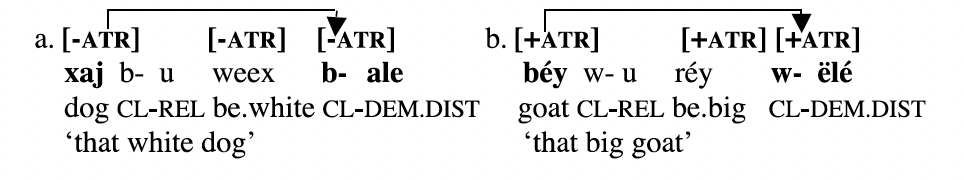
\includegraphics[scale = 0.65]{images/wolof.png}
\end{exe}
\begin{tikzpicture}[remember picture, overlay, >={Triangle[]}]
	\draw [->] (SyExatr1) |- ++(1,0.5) -| (SyExatr2);
	\draw [->] (SyExatr3) |- ++(1,0.5) -| (SyExatr4);
\end{tikzpicture}


\subsection{Irregular imperfective converb}\label{section:morphophono:auxiliary:imperfective}
All the preceding data focused on the perfective converb suffix. This suffix shows an inconstant or variable form, with or without a final liquid: [-el/ɻ] or [-e]. Whether a liquid surfaces or not is based   on the presence and location of the auxiliary. We find exactly the same behavior in another suffix: the irregular imperfective [-i(s)]. 

For regular verbs and most irregular verbs, the imperfective converb is formed by adding the suffix \textit{-um} onto the verb root or stem. In contrast, there are two irregular verbs `to give' and `to come' which form their imperfective converb  by adding the suffix \textit{-is} to the infinitive (Table \ref{tab:imperfective converb regular irregular ofrms}). Paradigms for these irregular verbs are given in \S\ref{section:verb:irregular:suppletive}.\footnote{{\seaSEA} utilizes the same irregular imperfective forms for the verbs `to come' [ɡ-ɑ-l],  `to give' [t-ɑ-l], and  `to cry' [l-ɑ-l].  But in {\iaIA},  the verb [l-ɑ-l] `to cry'   is replaced by regular [lɒt͡sʰ-e-l] `to cry' which forms its imperfective converb with \textit{-um}: [lɒt͡sʰ-um]. See \S\ref{section:verb:irregular:other} for discussion of  this verb.}

\begin{table}
	\caption{Formation of regular and irregular imperfective converbs}
	\label{tab:imperfective converb regular irregular ofrms}
% 	\resizebox{\textwidth}{!}{%
		\begin{tabular}{l ll lll}
			\lsptoprule
			& \multicolumn{2}{c}{Regular} &  \multicolumn{3}{c}{Irregular} \\\cmidrule(lr){2-3}\cmidrule(lr){4-6}
			&  \multicolumn{2}{l}{`to sing'} &  `to give' &  \multicolumn{2}{l}{`to come'} \\\midrule
			\textsc{inf} & jeɻkʰ-e-l &  $\sqrt{}$-{\thgloss}-{\infgloss}& t-ɒ-l & ɡ-ɒ-l &  $\sqrt{}$-{\thgloss}-{\infgloss}\\
			& \armenian{երգել} & & \armenian{տալ} & \armenian{գալ} & \\\addlinespace
			{\impfcvb} & jeɻkʰ-um&  $\sqrt{}$-{\impfcvb} & t-ɒ-l-is & ɡ-ɒ-l-is &  $\sqrt{}$-{\thgloss}-{\infgloss}-{\impfcvb}\\
			& \armenian{երգում} & & \armenian{տալիս} & \armenian{գալիս} & \\
			\lspbottomrule
		\end{tabular}%
% 	}
\end{table}


In \S\ref{section:morphophono:auxiliary:syntax}, we saw that the regular suffix \textit{-um} has a constant form and never alternates. In contrast,  the  irregular suffix  surfaces  as \textit{-is}   before the auxiliary, and as \textit{-i} when the auxiliary has shifted leftwards (\ref{sent:MorphoPhono:Liqid:IrrgImpf:ex}). 



\begin{exe}
	\ex \label{sent:MorphoPhono:Liqid:IrrgImpf:ex}
	\begin{xlist}
		\ex \gll jes  ɡiɻkʰ-ə  \uline{\textbf{t-ɒ-l-is}}  \colorbox{lsLightGray}{=e-m}
		\\
		I  book-{\defgloss}  give-{\thgloss}-{\infgloss}-{\impfcvb}  ={\auxgloss}-1{\sg}
		\\
		\trans `I am giving the book.' \hfill (NK)
		\\
		\armenian{Ես գիրքը տալիս եմ։}  
		\ex \gll jes  ɡiɻkʰ-ə \textbf{t͡ʃʰ\colorbox{lsLightGray}{-e-m}}  \uline{{t-ɒ-l-i}}  
		\\
		I  book-{\defgloss}    {\neggloss}={\auxgloss}-1{\sg} give-{\thgloss}-{\infgloss}-{\impfcvb}
		\\
		\trans `I am not giving  the book.' \hfill (NK)
		\\
		\armenian{Ես գիրքը չեմ  տալի։}
		\ex \gll jes  \textbf{ɡiɻkʰ} \colorbox{lsLightGray}{=e-m}  \uline{{t-ɒ-l-i}}  
		\\
		I  book    ={\auxgloss}-1{\sg} give-{\thgloss}-{\infgloss}-{\impfcvb}
		\\
		\trans `I am giving  books.'   \hfill (NK)
		\\
		\armenian{Ես գիրք եմ տալի։}
		\ex \gll \textbf{jes} \colorbox{lsLightGray}{=e-m}  ɡiɻkʰ-ə     \uline{{t-ɒ-l-i}}  
		\\
		I  {\auxgloss}-1{\sg} book-{\defgloss}   give-{\thgloss}-{\infgloss}-{\impfcvb}
		\\
		\trans `\textbf{\uline{I}} am  giving  the book.' \hfill (NK)
		\\
		\armenian{Ես եմ գիրքը   տալի։}
	\end{xlist}
\end{exe}

The imperfective [-is]$\sim$[-i] alternation happens in the same contexts as the perfective [-el/ɻ]$\sim$[-e] alternation. 	We report additional data from AS's work (\ref{sent:MorphoPhono:Liqid:IrrgImpf:AS}). The same generalization stands: if the auxiliary has shifted leftwards, then the suffix [-is] alternates with [-i].

\begin{exe}
	\ex\label{sent:MorphoPhono:Liqid:IrrgImpf:AS}
	\begin{xlist}
		\ex \gll \textbf{uʃ}  \colorbox{lsLightGray}{=e-n}   \uline{ɡ-ɒ-l-i}
		\\
		late ={\auxgloss}-3{\pl} come-{\thgloss}-{\infgloss}-{\impfcvb} 
		\\
		\trans `They are coming late.' \hfill (AS)
		\\
		\armenian{Ուշ են գալի։}
		\ex \gll \textbf{mez}  \colorbox{lsLightGray}{=e-n}   \uline{t-ɒ-l-i}
		\\
		us.{\dat} ={\auxgloss}-3{\pl} give-{\thgloss}-{\infgloss}-{\impfcvb} 
		\\
		\trans `They are giving it to us.' \hfill (AS)
		\\
		\armenian{Մեզ են տալի։}
		\ex \gll jes d͡zez-i \textbf{χoskʰ}  \colorbox{lsLightGray}{=e-m}   \uline{t-ɒ-l-i} voɻ ɒχt͡ʃʰik-əs el jeɻpʰekʰ sent͡sʰ bɒn-er t͡ʃʰ-i-$\emptyset$ ɒn-e-l-u
		\\
		I you.{\pl}-{\dat} promise ={\auxgloss}-3{\pl} give-{\thgloss}-{\infgloss}-{\impfcvb} that daughter-{\possFsg}  ever never these thing-{\pl} {\neggloss}-{\auxgloss}-3{\sg} do{\thgloss}-{\infgloss}-{\futcvb}
		\\
		\trans `I promise you that my daughter will never do these things.'  \hfill (AS)
		\\
		\armenian{Ես ձեզի խօսք եմ տալի որ աղջիկս էլ երբէք սենց բաներ չի անելու։} 
	\end{xlist}
\end{exe}




We likewise see the same long-distance conditions in reduced coordination (\ref{sent:MorphoPhono:Liqid:IrrgImpf:Coord}). The suffix surfaces as [-is] when the auxiliary is to the right within the phrase, even if not adjacent to the suffix. The suffix surfaces as [-i] when the auxiliary shifts leftwards.\largerpage


\begin{exe}
	\ex \label{sent:MorphoPhono:Liqid:IrrgImpf:Coord}
	\begin{xlist}
		\ex \gll \uline{{t-ɒ-l-is}} \colorbox{lsLightGray}{=e-m} kɒm \uline{{t͡sɒχ-um}} \colorbox{lsLightGray}{=e-m} \\
		give-{\thgloss}-{\infgloss}-{\impfcvb} ={\auxgloss}-1{\sg} or sell-{\impfcvb} ={\auxgloss}-1{\sg}
		\\
		\trans `I am giving or I am selling.' \hfill (NK)
		\\
		\armenian{Տալիս եմ կամ ծախում եմ։}
		\ex \gll \uline{{t-ɒ-l-is}}        kɒm \uline{{t͡sɒχ-um}} \colorbox{lsLightGray}{=e-m} \\
		give-{\thgloss}-{\infgloss}-{\impfcvb}     or sell-{\impfcvb} ={\auxgloss}-1{\sg}
		\\
		\trans `I am giving or selling.' \hfill (NK)
		\\
		\armenian{Տալիս  կամ ծախում եմ։}
  \ex \gll \textbf{t͡ʃʰ\colorbox{lsLightGray}{-e-m}} \uline{{t-ɒ-l-i}}        kɒm \uline{{t͡sɒχ-um}}  \\
		{\neggloss}={\auxgloss}-1{\sg} give-{\thgloss}-{\infgloss}-{\impfcvb}     or sell-{\impfcvb} 
		\\
		\trans `I am not giving or selling.' \hfill (NK)
		\\
		\armenian{Չեմ տալի   կամ ծախում ։}
\end{xlist}	\end{exe}




\subsection{Diachronic origins and effects of adjacency}\label{section:morphophono:auxiliary:EA}\largerpage

The previous section examined the synchronic behavior of the perfective converb suffix \textit{-el/eɻ} and how this suffix loses its liquid when the auxiliary has shifted. This section  describes the diachronic origins of this behavior in Standard and {\seaCEA}. 



In {\seaSEA}, the perfective converb suffix is \textit{-el}, and   the irregular imperfective converb suffix is \textit{-is}. Whereas these suffixes alternate in {\iaIA}, they do not  in {\seaSE} (\ref{sent:MorphoPhono:Liqid:History:sea}). The forms of the suffixes remain constant regardless of whether the auxiliary has shifted leftwards. 

\begin{exe}
	\ex Constant forms in {\seaSEA}\label{sent:MorphoPhono:Liqid:History:sea}
	\begin{xlist}
		\ex \gll \textbf{\uline{ɡəɾ-el}} \colorbox{lsLightGray}{=e-m}, \textbf{\uline{t-ɑ-l-is}} \colorbox{lsLightGray}{=e-m}
		\\
		write-{\perfcvb} ={\auxgloss}-1{\sg}, give-{\thgloss}-{\infgloss}-{\impfcvb} ={\auxgloss}-1{\sg}
		\\
		\trans `I have written, I am giving.'
		\\
		\armenian{Գրել եմ, տալիս եմ։}
		\ex \gll \textbf{t͡ʃʰ\colorbox{lsLightGray}{-e-m}} \uline{ɡəɾ-el}, \textbf{t͡ʃʰ\colorbox{lsLightGray}{-e-m}} \uline{t-ɑ-l-is}  
		\\
		{\neggloss}={\auxgloss}-1{\sg} write-{\perfcvb}, {\neggloss}={\auxgloss}-1{\sg} give-{\thgloss}-{\infgloss}-{\impfcvb}  
		\\
		\trans `I have not written, I am not giving.'
		\\
		\armenian{Չեմ գրել, չեմ  տալիս։}
	\end{xlist}
\end{exe}

\begin{sloppypar}
The {\iaIA} suffix [-el/-eɻ] developed from the  same historical source as the  {\seaSE} suffix. It is reported that across Armenian lects, the liquid of the perfective suffix    can sometimes change from /l/ to a rhotic (\citealt{grigoryan-2018-FallOfLiquidLPastParticipleInversionSpokenLanguage}; dialectological feature \#85 in \citealt[101]{Jahukyan-1972-ArmenianDiaolectology}). 
\end{sloppypar}

However, in {\seaCEA} (\seaCEAAbbre)  as spoken in Yerevan, it is reported that speakers can optionally drop the liquid /l/ and the fricative /s/ when the auxiliary has shifted (\ref{sent:MorphoPhono:Liqid:History:cea}) (\citealt[101]{Gharagyulyan-1981-ColloquialArmenian}, \citealt[213, 223]{DumTragut-2009-ArmenianReferenceGrammar}, \citealt[37]{KhamoyanEtAl-2014-ColloquialYerevanLanguage}).\pagebreak


\begin{exe}
	\ex Optional deletion in {\seaCEA}\label{sent:MorphoPhono:Liqid:History:cea}
	\begin{xlist}
		\ex \gll \textbf{\uline{ɡəɾ-el}} \colorbox{lsLightGray}{=e-m}, \textbf{\uline{t-ɑ-l-is}} \colorbox{lsLightGray}{=e-m}
		\\
		write-{\perfcvb} ={\auxgloss}-1{\sg}, give-{\thgloss}-{\infgloss}-{\impfcvb} ={\auxgloss}-1{\sg}
		\\
		\trans `I have written, I am giving.'
		\\
		\armenian{Գրել եմ, տալիս եմ։}
		\ex \gll \textbf{t͡ʃʰ\colorbox{lsLightGray}{-e-m}} \uline{ɡəɾ-e(l)}, \textbf{t͡ʃʰ\colorbox{lsLightGray}{-e-m}} \uline{t-ɑ-l-i(s)}  
		\\
		{\neggloss}={\auxgloss}-1{\sg} write-{\perfcvb}, {\neggloss}={\auxgloss}-1{\sg} give-{\thgloss}-{\infgloss}-{\impfcvb}  
		\\
		\trans `I have not written, I am not giving.'
		\\
		\armenian{Չեմ գրել, չեմ  տալիս։}
	\end{xlist}
\end{exe}

The deletion of the final liquid   is reported to be unique to the perfective converb suffix  [-el] in {\seaCEA}. This colloquial process is likewise attested in the {\seaCEA}   spoken by immigrant communities in Los Angeles  \citep[72]{Karapetian-2014-TeachArmenianEasternArmenianHeritage}. 


There is some experimental evidence   that this optional deletion process in {\seaCEA} is related to   the prosodic weakening of liquids \citep{grigoryan-2018-FallOfLiquidLPastParticipleInversionSpokenLanguage}.  


One speaker of {\seaCEAAbbre} (VP)    informed us that the clitic [=el] `also, even' can also optionally delete its liquid in {\seaCEAAbbre} (\ref{sent:MorphoPhono:Liqid:History:ceaOther}). 

\begin{exe}
	\ex {\seaCEA}\\ \gll jes e(l) kʰez =e-m spɑs-um 
	\\
	I also you.{\sg}.{\dat} ={\auxgloss}-1{\sg} wait-{\impfcvb}
	\\
	\trans `I am also waiting for you.' \hfill (VP) \label{sent:MorphoPhono:Liqid:History:ceaOther}
	\\
	\armenian{Ես էլ քեզ եմ սպասում։}
\end{exe}


For {\seaCEA}, we  asked young speakers from Armenia (around 20--40 years old) for their sociolinguistic intuitions about the optional deletion in the suffixes [-el] and [-is] (Table \ref{tab:coll ea judgment people}). Some speakers told us that they themselves have this optional process in their speech, some told us they do not do it at all. Some told us that this process is common, while others told us that it is judged as “vulgar” and uncommon. Some told us that they can apply the deletion in some verbs, but not others.\largerpage

\vfill
\begin{table}[H]
	\caption{Consultants on {\seaCEA} and their meta-linguistic judgments\label{tab:coll ea judgment people}}
	\resizebox{\textwidth}{!}{%
		\begin{tabular}{lllll}
			\lsptoprule
			Speaker& Age& Sex & What verbs? & Social judgment? \\\midrule
			MA & late-20s & F &   `open', `close', `eat', `drink' & ``it's colloquial''\\
			VP & mid-30s & M & any verb & ``any social class/region''\\
			HH & early-20s & M & N/A & ``it's colloquial and vulgar''\\ 
			\lspbottomrule
		\end{tabular}
	}
\end{table}
\vfill\pagebreak

The above reports suggest that this colloquial process is attested but stigmatized. The use of this process varies by speaker, and sometimes by   verb. There is little to no work on the variationist sociolinguistics of Armenian,\footnote{To our knowledge, the closest work is Zakaryan  \citep{Zakaryan-1981-ColloquialArmenian}, a study of social factors in different Armenian morphophonological choices.}   so we do not know if any demographic factors are correlated with this deletion process.



Diachronically,  there is an obvious path of historical development for the perfective suffix in {\iaIA}. 1) In some stage of the dialect, there was no deletion at all  [-el] (like modern {\seaSEA}). 2) Later on, the dialect developed optional deletion [-e(l)] (like modern  {\seaCEA}). 3)   Finally, the deletion became obligatory [-e] (as in modern {\iaIA}).  As we   discuss below, stages 2 (for {\seaCEAAbbre}) and 3 (for {\iaAbbre}) also seem to differ in terms of adjacency requirements between the suffix and the auxiliary. 

%{\added}


		Data on this colloquial process is sparse, but we suspect that {\seaCE} and {\iaIA} differ in the role of adjacency between the verb and auxiliary. Briefly, in {\iaIA}, non-adjacent auxiliaries cause the liquid to surface, while non-adjacent auxiliaries can cause the liquid to delete. We illustrate below. 

Consider the sentences in (\ref{colloq coordination el base unreduced reduced}), in both {\seaCE} and   {\iaIA}. In (\ref{colloq coordination el base unreduced reduced: unreduced}), the sentence has un-reduced coordination with two verbs and two auxiliaries. The verb's liquid surfaces in both dialects. But in   reduced coordination (\ref{colloq coordination el base unreduced reduced: reduced}) with just one auxiliary, Verb1 keeps its liquid in {\iaIA} but can optionally delete it in {\seaCEA}. No deletion is found in {\seaSE}. We use -\textsc{p}, ={\auxgloss} instead of -{\perfcvb}, ={\auxgloss}-1{\sg}.\largerpage[-2]

\begin{exe}
	\ex Effect of verb-auxiliary adjacency in {\seaCE} and   {\iaIA}\label{colloq coordination el base unreduced reduced}
	
	\begin{xlist}
		\ex Un-reduced coordination with two auxiliaries\label{colloq coordination el base unreduced reduced: unreduced}\\
		\begin{tabular}{@{}l llllll l@{}}
			& Verb1 & Aux  & Conj & Verb2 & Aux 
			\\
			i. & \uline{χəm-el} & \colorbox{lsLightGray}{=e-m}& kɑm & \uline{keɾ-el} & \colorbox{lsLightGray}{=e-m} & ({\seaAbbre})  & (MA, VP)\\
			
			ii. & \uline{χəm-el} &\colorbox{lsLightGray}{=e-m}& kɑm & \uline{keɾ-el} &\colorbox{lsLightGray}{=e-m} & ({\seaCEAAbbre}) &  (MA, VP)   \\
			& \multicolumn{5}{l}{\armenian{Խմել եմ կամ կերել եմ։}}  & 
			\\
			iii. & \uline{χəm-eɻ} & \colorbox{lsLightGray}{=e-m}& kɒm & \uline{keɻ-eɻ} & \colorbox{lsLightGray}{=e-m}& ({\iaAbbre}) & (NK)\\
			& drink-\textsc{p} & ={\auxgloss} & or & eat-\textsc{p}& ={\auxgloss} & 
			\\
			& \multicolumn{5}{l}{`I have drunk or have eaten.'}  & 
			\\
			& \multicolumn{5}{l}{\armenian{Խմեր եմ կամ կերեր եմ։}}  & 
		\end{tabular}
		\pagebreak\ex Reduced coordination with one auxiliary\label{colloq coordination el base unreduced reduced: reduced}\\
		\begin{tabular}{@{}l llllll l@{}}
			& Verb1 &   & Conj & Verb2 & Aux
			\\
			i. & \uline{χəm-el} & ~~~~~~~~~~~          & kɑm & \uline{keɾ-el} & \colorbox{lsLightGray}{=e-m} & ({\seaAbbre})  &  (MA, VP) \\
			ii. & \uline{χəm-e(l)} &\ & kɑm & \uline{keɾ-el} &\colorbox{lsLightGray}{=e-m} & ({\seaCEAAbbre})  & (MA, VP) \\
			& \multicolumn{5}{l}{\armenian{Խմել  կամ կերել եմ։}}  & 
			\\
			
			iii. & \uline{χəm-eɻ} & & kɒm & \uline{keɻ-eɻ} & \colorbox{lsLightGray}{=e-m}& ({\iaAbbre}) & (NK)	\\
			& drink-\textsc{p} &   & or & eat-\textsc{p}& ={\auxgloss} & 
			\\
			& \multicolumn{5}{l}{`I have drunk or   eaten.'}  & 
			\\
			& \multicolumn{5}{l}{\armenian{Խմեր  կամ կերեր եմ։}}  & 
		\end{tabular}
		
	\end{xlist}
\end{exe}




When reduced coordination is negated, {\seaSE} keeps the liquid in Verb1, while   {\iaIA} deletes the liquids in both Verb1 and Verb2 (\ref{ex:morphophono:liq:diach:ceanegkam}). For {\seaCEA}, either both liquids surface or both delete. Other permutations are not possible for our informants (liquid + no liquid, no liquid + liquid). 



\begin{exe}
	\ex Reduced coordination with negation and consonant-initial conjunction\label{ex:morphophono:liq:diach:ceanegkam}\\	
	\begin{tabular}{l llllll l}
		& Neg-Aux & Verb1 &     Conj & Verb2 &
		\\
		i. & \textbf{t͡ʃʰ\colorbox{lsLightGray}{-e-m}}&  \uline{χəm-el}         & kɑm & \uline{keɾ-el}  & ({\seaAbbre})  & (MA, VP) \\
		ii. & \textbf{t͡ʃʰ\colorbox{lsLightGray}{-e-m}}& \uline{χəm-el}    & kɑm & \uline{keɾ-el}   & ({\seaCEAAbbre}) &  (MA, VP) \\
		& \textbf{t͡ʃʰ\colorbox{lsLightGray}{-e-m}}& \uline{χəm-e}    & kɑm & \uline{keɾ-e}   &  & (MA, VP) \\
		& *\textbf{t͡ʃʰ\colorbox{lsLightGray}{-e-m}}& \uline{χəm-e}    & kɑm & \uline{keɾ-el}   &  & (*MA, *VP) \\
		& *\textbf{t͡ʃʰ\colorbox{lsLightGray}{-e-m}}& \uline{χəm-el}    & kɑm & \uline{keɾ-e}   &  & (*MA, *VP) \\
		& \multicolumn{5}{l}{\armenian{Չեմ խմել  կամ կերել։}}  & 
		\\
		
		iii. & \textbf{t͡ʃʰ\colorbox{lsLightGray}{-e-m}}& \uline{χəm-e} &  kɒm & \uline{keɻ-e}  & ({\iaAbbre}) & (NK)	\\
		& {\neggloss}={\auxgloss}& drink-\textsc{p} &     or & eat-\textsc{p} & 
		\\
		& \multicolumn{5}{l}{`I have not drunk or   eaten.'}  & 
		\\
		& \multicolumn{5}{l}{\armenian{Չեմ խմէ կամ կերէ։}} & 
	\end{tabular}
	
\end{exe}






The generalization so far is the following. In both {\iaIA} and {\seaCEA}, the auxiliary licenses the floating liquid of the perfective converb. In {\iaIA}, the suffix and auxiliary do not need to be adjacent, but they do need to be adjacent in {\seaCEA}.% We can formalize this variation with the following rules, adapted from Rule \ref{fig:docking perf v2}. 
%
%\begin{ruleblock}
%	{\textbf{Liquid retention}: Dialect variation for the morpheme-specific rule of anchoring (surfacing) floating segments before the auxiliary}
%	\label{fig:docking perf v2 eas}
%	
%	\begin{center}
%		\begin{tabular}{|llll|llll|  }
%			\hline 
%			\multicolumn{4}{| l| }{{\iaAbbre} } & \multicolumn{4}{| l| }{{\seaCEAAbbre} }
%			\\
%			\multicolumn{4}{| l| }{Non-adjacent conditioning } & \multicolumn{4}{| l| }{Adjacent conditioning}
%			\\
%			
%			$<$C$>$ & $\rightarrow$  & C & / [ \_ $\dots$ {\auxgloss} ]
%			& 
%			$<$C$>$ & $\rightarrow$  & C & / [ \_   {\auxgloss} ]
%			\\
%			\hline 
%			
%		\end{tabular}
%		
%	\end{center}	
%\end{ruleblock}

The above generalization  is however too simplified for   {\seaCEA}, because we have found some variation across speakers. In reduced coordination with a vowel-initial conjunction, one {\seaSE} speaker  told us that they can delete the liquid on Verb1 (VP), while another said that they could not (MA). This data suggests that some speakers can allow other adjacent vowel-initial words to license the perfective liquid (\ref{ex:morphophono:liq:diach:ceaVword}). 



\begin{exe}
	\ex Effect of other vowel-initial words   in {\seaCEA} and in {\iaIA}\label{ex:morphophono:liq:diach:ceaVword}
	
	\begin{xlist}
		\ex Un-reduced coordination with two auxiliaries
		
		\begin{tabular}{@{}l llllll l@{}}
			& Verb1 & Aux  & Conj & Verb2 & Aux\\
			i. & \uline{χəm-el} & \colorbox{lsLightGray}{=e-m}& u & \uline{keɾ-el} & \colorbox{lsLightGray}{=e-m} & ({\seaAbbre})  & \\
			ii. & \uline{χəm-el} &\colorbox{lsLightGray}{=e-m}& u & \uline{keɾ-el} &\colorbox{lsLightGray}{=e-m} & ({\seaCEAAbbre})  \\
			& \multicolumn{5}{l}{\armenian{Խմել եմ ու կերել եմ։}}  & 
			\\
			
			iii. & \uline{χəm-eɻ} & \colorbox{lsLightGray}{=e-m}& u & \uline{keɻ-eɻ} & \colorbox{lsLightGray}{=e-m}& ({\iaAbbre}) & (NK) 	\\
			& drink-\textsc{p} & ={\auxgloss} & and & eat-\textsc{p}& ={\auxgloss} & 
			\\
			& \multicolumn{5}{l}{`I have drunk and have eaten.'}  & 
			\\
			& \multicolumn{5}{l}{\armenian{Խմեր եմ ու կերեր եմ։}}  & 
		\end{tabular}
		\ex Reduced coordination with one auxiliary
		
		\begin{tabular}{@{}l llllll l@{}}
			& Verb1 &   & Conj & Verb2 & Aux
			\\
			i. & \uline{χəm-el} & ~~~~~~~~~~~          & u & \uline{keɾ-el} & \colorbox{lsLightGray}{=e-m} & ({\seaAbbre})  & (MA, VP) \\
			ii. & \uline{χəm-el} &\ & u & \uline{keɾ-el} &\colorbox{lsLightGray}{=e-m} & ({\seaCEAAbbre})  &  (VP, MA) \\
			& \uline{χəm-e} &\ & u & \uline{keɾ-el} &\colorbox{lsLightGray}{=e-m} & ({\seaCEAAbbre})  &  (VP, *MA)\\
			& \multicolumn{5}{l}{\armenian{Խմել  կամ կերել եմ։}}  & 
			\\
			
			iii. & \uline{χəm-eɻ} & & u & \uline{keɻ-eɻ} & \colorbox{lsLightGray}{=e-m}& ({\iaAbbre}) & (NK) 	\\
			& drink-\textsc{p} &   & and & eat-\textsc{p}& ={\auxgloss} & 
			\\
			& \multicolumn{5}{l}{`I have drunk and   eaten.'}  & 
			\\
			& \multicolumn{5}{l}{\armenian{Խմեր  ու կերեր եմ։}}  & 
		\end{tabular}
		
	\end{xlist}
\end{exe}

The variation can cause ineffability      when reduced coordination involves negation and a vowel-initial conjunction (\ref{ex:morphophono:liq:diach:ceaVConjNeg}). In the sentences below, the auxiliary has to shift because of negation, and Verb1 precedes a vowel. Our consultants VP and MA are fine with deleting neither liquid. VP is fine with deleting both  liquids, but MA is not. Neither speaker is fine with deleting only one liquid.  For {\iaIA}, our main consultant required deletion in both verbs. However, another speaker (GE) reports that deletion of the first liquid is optional. 


\begin{exe}
	\ex Reduced coordination with negation and vowel-initial conjunction\label{ex:morphophono:liq:diach:ceaVConjNeg}
	
	\begin{tabular}{l llllll l}
		& Neg-Aux & Verb1 &     Conj & Verb2 &
		\\
		i. & \textbf{t͡ʃʰ\colorbox{lsLightGray}{-e-m}}&  \uline{χəm-el}         & u & \uline{keɾ-el}  & ({\seaAbbre})  & (VP, MA) \\
		ii. & \textbf{t͡ʃʰ\colorbox{lsLightGray}{-e-m}}& \uline{χəm-el}    & u & \uline{keɾ-el}   & ({\seaCEAAbbre}) &  (VP, MA) \\
		& \textbf{t͡ʃʰ\colorbox{lsLightGray}{-e-m}}& \uline{χəm-e}    & u & \uline{keɾ-e}   &  & (VP, *MA) \\
		& *\textbf{t͡ʃʰ\colorbox{lsLightGray}{-e-m}}& \uline{χəm-e}    & u & \uline{keɾ-el}   &  & (*VP, *MA) \\
		& *\textbf{t͡ʃʰ\colorbox{lsLightGray}{-e-m}}& \uline{χəm-el}    & u & \uline{keɾ-e}   &  & (*VP, *MA) \\
		& \multicolumn{5}{l}{\armenian{Չեմ խմել  ու կերել։}}  & 
		\\
	\end{tabular}\\
	\begin{tabular}{l llllll l}
		iii. & \textbf{t͡ʃʰ\colorbox{lsLightGray}{-e-m}}& \uline{χəm-e} &  u & \uline{keɻ-e}  & ({\iaAbbre}) & (NK) 	\\
		   & \textbf{t͡ʃʰ\colorbox{lsLightGray}{-e-m}}& \uline{χəm-e(l)} &  u & \uline{keɻ-e}  & ({\iaAbbre}) & (GE) 	\\
				& {\neggloss}={\auxgloss}& drink-\textsc{p} &     and & eat-\textsc{p} & 
		\\
		& \multicolumn{5}{l}{`I have not drunk and   eaten.'}  & 
		\\
		& \multicolumn{5}{l}{\armenian{Չեմ խմէ ու կերէ։}} & 
	\end{tabular}
\end{exe}

The data from {\seaCEA} and {\iaIA} is  quite complicated and our analysis is incomplete. More variation-oriented data is required from larger pools of people from different areas and  generations.  But crucially, the overarching generalization is that whereas {\iaAbbre} allows non-local conditioning between the suffix and the auxiliary, {\seaCEAAbbre} seems to require local conditioning.   Some {\iaAbbre} speakers also allow both generalizations simultaneously (non-local or local conditioning).


\chapter{Nominal morphology}\label{chapter:noun}


This chapter covers   the basics of nominal inflection in {\iaIA}. In general, we have not found any significant differences between {\seaSE} and {\iaIA} in this domain. We thus keep this chapter brief, with an overview of the basic paradigms. For larger paradigms and for work on the noun phrase of Armenian, we refer readers to other sources for {\seaSEA} (\cites{Kozintseva-1995-EasternBook}{Yeghiazaryan-2010-ArmenianCase}[\S4]{Tamrazian-1994-ArmenianSyntax}[\S5]{Megerdoomian-2009-ThesisBook}[\S2.1]{DumTragut-2009-ArmenianReferenceGrammar}[\S2.1.1]{Hodgson-2019-DissRelativeClauseArmenianSyntax}) and {\swaSWA} (\cites{Sigler-1997-SpecificitySWADissertation}[\S2.3]{Khanjian-2013-DissNegativeConcord}{BaleKhanjian-2014-SyntacticComplexityCompetitionSingularPluralWesternArmenian}).


\section{Basic template for nominal inflection}\label{section:noun:template}

Nominal inflection is agglutinative for number, case, possession, and definite marking. The basic template for   nominal inflection is given in Table \ref{tab:template noun}. The rightmost column is dedicated to possessive and definiteness marking, which we refer to collectively as a Determiner slot. We list productive suffixes within each cell, including suffixal allomorphs.

\begin{table}
	\caption{Template for nominal inflection and the set of productive suffixes}
	\label{tab:template noun}
	\begin{tabular}{ l lllll lll l  }
		\lsptoprule 
		N & \multicolumn{3}{c}{Number} & \multicolumn{3}{c}{Case ({\case})} & \multicolumn{3}{c}{Determiner ({\detgloss})}\\ \cmidrule(lr){2-4}\cmidrule(lr){5-7}\cmidrule(lr){8-10}
		& {\sg} & -$\emptyset$& & {\nom}/{\acc} &-$\emptyset$& & unmarked & -$\emptyset$&\\
		& {\pl} & {-eɻ} & \armenian{-եր} & {\dat}/{\gen} & {-i}& \armenian{-ի} & {\possFsg}& {-(ə)s}& \armenian{-ս}\\
		&& {-neɻ} & \armenian{-ներ} & {\abl}& {-it͡sʰ}& \armenian{-ից} & {\possSsg}& {-(ə)t} & \armenian{-դ}\\ 
		& & && {\ins}& {-ov} &\armenian{-ով}& {\defgloss} & {-ə}& \armenian{-ը}\\
		&& & & {\locgloss}& {-um}& \armenian{-ում} & & {-n}& \armenian{-ն}\\
		& & & & & & & & {-ən}&\armenian{-ն}\\
		\lspbottomrule 
	\end{tabular}
\end{table}


Some of the above morphemes have multiple realizations due to pho\-nol\-o\-gi\-cal\-ly-con\-di\-tioned allomorphy. Such allomorphy is discussed in \S\ref{section:morphophono:allomorphy}.


To illustrate nominal inflection, we show the paradigms of a singular case-marked noun, a plural case-marked noun, and a plural case-marked possessed noun (Table \ref{tab:noun basic paradigm}). Note that possessive marking follows   case marking. 

\begin{table}
	\caption{Paradigm for singular noun, plural noun, and plural possessed noun}
	\label{tab:noun basic paradigm}
	\begin{tabular}{ ll l l }
		\lsptoprule 
		& N-{\case} & N-{\pl}-{\case} & N-{\pl}-{\case}-{\possFsg}\\\midrule
		{\nom}/{\acc} & {senjɒk}& {senjɒk-neɻ} & {senjɒk-neɻ-əs}\\
		&\armenian{սենեակ} &\armenian{սենեակներ} &\armenian{սենեակներս}\\
		\addlinespace 
		{\dat}/{\gen} & {senjɒk-i} & {senjɒk-neɻ-i} & {senjɒk-neɻ-i-s} \\
		&\armenian{սենեակի}&\armenian{սենեակների}&\armenian{սենեակներիս}\\
		\addlinespace 
		{\abl} & {senjɒk-it͡sʰ} & {senjɒk-neɻ-it͡sʰ} & {senjɒk-neɻ-it͡sʰ-əs}\\
		&\armenian{սենեակից}
		&\armenian{սենեակներից}
		&\armenian{սենեակներիցս}\\
		\addlinespace 
		{\ins} & {senjɒk-ov} & {senjɒk-neɻ-ov} & {senjɒk-neɻ-ov-əs}\\
		&\armenian{սենեակով}
		&\armenian{սենեակներով}
		&\armenian{սենեակներովս}\\
		\addlinespace 
		{\locgloss} & {senjɒk-um} & {senjɒk-neɻ-um} & {senjɒk-neɻ-um-əs} \\
		&\armenian{սենեակում}
		&\armenian{սենեակներում}
		&\armenian{սենեակներումս}\\
		\addlinespace 
		& `room' &`rooms'&`my rooms'\\
		\lspbottomrule
	\end{tabular}
	
\end{table}

In {\seaSEA}, the word for `case' is /holov/ \armenian{հոլով}. The names of the different cases are in Table \ref{tab:case name}.\largerpage

\begin{table}
	\caption{Names of cases in {\seaSEA}}
	\label{tab:case name}
	\begin{tabular}{lll}
		\lsptoprule
		Nominative & uʁʁɑkɑn  &  \armenian{ուղղական}\\
		Accusative &hɑjt͡sʰɑkɑn  &  \armenian{հայցական}\\
		Genitive &  serɑkɑn & \armenian{սեռական}\\
		Dative &  təɾɑkɑn  & \armenian{տրական}\\
		Ablative &  bɑt͡sʰɑrɑkɑn & \armenian{բացառական}\\
		Instrumental &  ɡoɾt͡sijɑkɑn  & \armenian{գործիական}\\
		Locative & neɾɡojɑkɑn  &  \armenian{ներգոյական}\\ 
		\lspbottomrule  
		\end{tabular}
\end{table}

In terms of syncretism and exponence, nominative and accusative are zero-marked, singular number is unmarked, and dative and genitive are syncretic for common nouns. However, this syncretism     does not apply to personal pronouns, which we discuss in \S\ref{section:funct:personal pronoun}.

{\seaSEA} can use  the instrumental case marker \textit{-ov} to denote either the meaning of `to use X as an instrument' or `to go along with X'. The latter meaning is considered a comitative meaning \citep[93]{DumTragut-2009-ArmenianReferenceGrammar}. {\swaSWA} can likewise use the instrumental as a comitative. However in {\iaIA}, the comitative meaning of the instrumental suffix is considered atypical and odd. Speakers prefer to express the comitative meaning through an alternative postpositional construction.\footnote{%{\added}
	However, a reviewer  states that a possibly more accurate description of {\seaAbbre} is that the instrumental can be used for activities that are carried out as a group (for example as a family), and not alongside a person. If we take this description of {\seaAbbre} as accurate, then both {\seaAbbre} and {\iaAbbre} lack comitative instrumentals, while {\swaAbbre} has them. However, KM did report that she encountered such comitative readings in {\seaAbbre} before, so it is possible that there is variation among {\seaAbbre} speakers. Our {\seaAbbre} consultant AT said that such a comitative  reading is ``not okay'' but that it is possible that someone might use it in a disparaging way, e.g., a misogynist might use the comitative instrumental of the word `sister'. }

For example, sentence (\ref{sentence inst comitative no}) places an instrumental suffix on the noun. The intended interpretation is comitative: to go along with the sister. Such a meaning is possible for some speakers in {\seaSEA}, but not in {\iaIA}. The typical {\iaIA} reading would be purely instrumental: to go to the cinema by using the sister. To express the comitative meaning, speakers strongly prefer using the postposition \textit{het} (\ref{sentence inst comitative yes}).\footnote{For the word `sister', the nominative form is [{kʰuɻ}] \armenian{քուր}. In the dative/genitive, the word uses an irregular allomorph for both the root and the suffix: [{kʰəɻ-ot͡ʃʰ}]. The dative/genitive stem is then further inflected to form the instrumental. Note that the prescriptive form of the irregular dative/genitive suffix is [{-od͡ʒ}], but in {\iaIA} it is more often pronounced as [{-ot͡ʃʰ}].}\largerpage

\begin{exe}
	\ex 
	\begin{xlist}
		\ex \gll {kʰəɻ-ot͡ʃʰ-ov-əs} {ɡən-ɒ-t͡sʰ-i-ŋkʰ} {sinemɒ} 
		\\
		sister-{\dat}-{\ins}-{\possFsg} go-{\thgloss}-{\aorperf}-{\pst}-1{\pl} cinema
		\\
		\trans 	Intended meaning: `We went to the cinema along with my sister.' \label{sentence inst comitative no}
		\\
		Actual meaning: `We went to the cinema by using my sister.'
		\\
		\armenian{Քրոջովս գնացինք սինեմա։} \hfill (KM)
		\ex \gll {kʰəɻ-ot͡ʃʰ-əs} {het} {ɡən-ɒ-t͡sʰ-i-ŋkʰ} {sinemɒ}
		\\
		sister-{\gen}-{\possFsg} with go-{\thgloss}-{\aorperf}-{\pst}-1{\pl} cinema
		\\
		\trans 	`We went to the cinema along with my sister.'\label{sentence inst comitative yes}
		\\
		\armenian{Քրոջս հետ գնացինք սինեմա։} \hfill (KM)
	\end{xlist}
\end{exe}



The   suffixes in Table \ref{tab:template noun} are the  regular  or default suffixes for the corresponding morphosyntactic features. {\iaIA} has limited     morphologically-conditioned allomorphy with irregular suffixes. We have not found any significant differences for irregular inflection in {\iaIA} vs. {\seaSEA}. At most, it seems that {\iaIA} is slowly leveling out irregular inflection.



To illustrate, the regular dative/genitive suffix is \textit{-i}. In both {\seaSE} and {\iaIA}, the dative/genitive suffix has a wide set of irregular allomorphs or realizations. For example, the suffix \armenian{-ութիւն} /{-utʰjun}/ is a productive nominalizer (\ref{sent:Noun:BasicTemplate:utʰjun}). This suffix forms an irregular dative/genitive by using a different allomorph for the entire nominalizer suffix: \armenian{-ութեան} /{-utʰjɒn}/. The use of this    allomorph is the prescriptive rule in {\seaSE} and {\iaIA}, but KM reports that {\iaIA} speakers much more frequently apply a regularized form /{-utʰjun-i}/. 



\begin{exe}
	\ex \textit{Leveling out of irregular dative/genitive of /{-utʰjun}/}
	\label{sent:Noun:BasicTemplate:utʰjun}
	
	\resizebox{\linewidth}{!}{%
		\begin{tabular}{@{}l@{~}llll@{}}
			a. & {uɻɒχ} & & `happy' & \armenian{ուրախ} \\
			& {uɻɒχ-utʰjun} & happy-{\nmlz} & `happiness' & \armenian{ուրախութիւն} \\
			b. & {uɻɒχ-utjɒn} & happy-{\nmlz}.{\dat}/{\gen} & `to/of happiness' & \armenian{ուրախութեան} \\
			c. & {uɻɒχ-utʰjun-i} & happy-{\nmlz}-{\dat}/{\gen} & `to/of happiness' &\armenian{ուրախութիւնի} \\
		\end{tabular}
	}
\end{exe}

For complete paradigms of these irregular declensions in {\seaSEA}, see \citet[\S2.1.2]{DumTragut-2009-ArmenianReferenceGrammar}. These paradigms apply to the formal prescriptive speech of {\iaIA}s.  But in casual speech, KM and AS report the loss of   various irregular case suffixes. 
\section{Constraints on definite marking and case marking}\label{section:noun:caseDefConstraint}


The determiner slot can be realized by either nothing, the 1SG possessive, 2SG possessive, or the definite suffix. The 1SG possessive  and 2SG possessive  can follow any type of case marker. This was illustrated in section \S\ref{section:noun:template} in Table \ref{tab:noun basic paradigm} for the 1SG possessive. However, the definite suffix cannot follow the genitive, ablative, or instrumental (\citealt[104]{DumTragut-2009-ArmenianReferenceGrammar}, \citealt[7]{Yeghiazaryan-2010-ArmenianCase}, \citealt[48]{Hodgson-2019-DissRelativeClauseArmenianSyntax}, \citeyear{Hodgson-202x-GrammaticaliztionDefiniteARticleArmenian}).\footnote{%{\added}
	We treat the definite and possessive morphemes as suffixes and not clitics. Morphosyntactically, there is no obvious evidence for treating them as separate words (clitics) instead of suffixes. Phonologically, these morphemes are unstressed (like clitics). But because these morphemes lack a non-schwa vowel, a suffix account already correctly predicts that they are unstressable (\S\ref{section:phono:suprasegmental:stress:reg}).   }


To illustrate, Table \ref{tab:def case restriction} shows definite marking on singular   and plural nouns. For the genitive, ablative, and instrumental, the noun is semantically ambiguous in terms of being definite or not. %{\added}
The gloss {\case} is a placeholder for case marking.\footnote{%{\added}
	The morpheme sequence of instrumental-definite is judged as ungrammatical by NK. In {\seaSEA} it is also judged as odd. However, BV found around 29 instances of this morpheme sequence as [senjɑk-um-ə] \armenian{սենյակումը} `in the room'   on the EANC. Victoria Khurshudyan reported that such a sequene can be uttered, ``but it will be clearly perceived as a non-standard form.''  }


\begin{table}
	\caption{Paradigm of definite singular noun and definite plural noun}
	\label{tab:def case restriction}
	\begin{tabular}{ll lll }
		\lsptoprule 
		& \makebox[.2cm][l]{}N-{\case}-{\defgloss} && \makebox[.2cm][l]{}N-{\pl}-{\case}-{\defgloss} & \\
		\midrule 
		{\nom}/{\acc} & \makebox[.2cm][l]{}{senjɒk-ə}&\armenian{սենեակը} & \makebox[.2cm][l]{}{senjɒk-neɻ-ə}&\armenian{սենեակնեըր}\\
		{\dat} & \makebox[.2cm][l]{}{senjɒk-i-n} &\armenian{սենեակին}& \makebox[.2cm][l]{}{senjɒk-neɻ-i-n} &\armenian{սենեակներին}\\
		{\gen} & \makebox[.2cm][l]{}{senjɒk-i} &\armenian{սենեակի}& \makebox[.2cm][l]{}{senjɒk-neɻ-i} &\armenian{սենեակների}\\
		& \makebox[.2cm][l]{*}{senjɒk-i-n} & & \makebox[.2cm][l]{*}{senjɒk-neɻ-i-n} & \\
		{\abl} & \makebox[.2cm][l]{}{senjɒk-it͡sʰ} &\armenian{սենեակից}& \makebox[.2cm][l]{}{senjɒk-neɻ-it͡sʰ} &\armenian{սենեակներից}\\
		& \makebox[.2cm][l]{*}{senjɒk-it͡sʰ-ə} & & \makebox[.2cm][l]{*}{senjɒk-neɻ-it͡sʰ-ə} & \\
		{\ins} & \makebox[.2cm][l]{}{senjɒk-ov} &\armenian{սենեակով}& \makebox[.2cm][l]{}{senjɒk-neɻ-ov} &\armenian{սենեակներով}\\
		& \makebox[.2cm][l]{*}{senjɒk-ov-ə} & & \makebox[.2cm][l]{*}{senjɒk-neɻ-ov-ə}& \\
		{\locgloss} & \makebox[.2cm][l]{}{senjɒk-um} &\armenian{սենեակում}& \makebox[.2cm][l]{}{senjɒk-neɻ-um}&\armenian{սենեակներում}\\
		& \makebox[.2cm][l]{*}{senjɒk-um-ə} & & \makebox[.2cm][l]{*}{senjɒk-neɻ-um-ə} & \\
		\midrule 
		& `the room' &&`the rooms'&\\
		\lspbottomrule
	\end{tabular}
\end{table}

It is interesting that the dative and genitive are syncretic with the suffix \textit{{-i}}. However, the definite suffix can be used after the dative form, but not the genitive form. This is illustrated in the following sentences.

In sentence (\ref{sentence:dative def}), the suffix \textit{{-i}} marks dative case. It can take the definite suffix \textit{{-n}}. But in (\ref{sentence:gen def}), the suffix \textit{{-i}} marks genitive case. It cannot be followed by the definite suffix.

\begin{exe}
	\ex 
	\begin{xlist}
		\ex \gll {senjɒk-i-n} {ɡiɻkʰ} {təv-ɒ-m}
		\\
		room-{\dat}-{\defgloss} book give-{\pst}-1{\sg}
		\\
		\trans	`I gave books to the room.' \hfill (NK)\label{sentence:dative def}
		\\
		\armenian{Սենեակին գիրք տուամ։}
		
		
		\ex \gll {senjɒk-i(*-n)} {ɡujn-ə}
		\\
		room-{\gen}-*{\defgloss} color-{\defgloss}
		\\
		\trans			`the color of the room' \hfill (*NK) \label{sentence:gen def}
		\\
		\armenian{սենեակի գոյնը}	\end{xlist}
	
\end{exe}

This co-occurrence restriction applies equally to both non-human nouns and to human nouns, such as the given name Aram (\ref{sent:Noun:Def:cooccurence}). 

\begin{exe}
	\ex \label{sent:Noun:Def:cooccurence}
	\begin{xlist}
		\ex \gll {ɒɻɒm-i-n} {ɡiɻkʰ} {təv-ɒ-m}
		\\
		Aram-{\dat}-{\defgloss} book give-{\pst}-1{\sg}
		\\
		\trans 	`I gave books to Aram.'\hfill (NK)
		\\
		\armenian{Արամին գիրք տուամ։}
		
		
		\ex \gll {ɒɻɒm-i(*-n)} {ɡiɻkʰ-ə}
		\\
		Aram-{\gen}-*{\defgloss} book-{\defgloss}
		\\
		\trans 			`the book of Aram'\hfill (NK)
		\\
		\armenian{Արամի գիրքը}
	\end{xlist}	
\end{exe}





The co-occurrence restriction between the genitive and the definite suffix is limited to just the definite suffix (\ref{sent:Noun:Def:cooccurencePoss}). Other determiner suffixes like the 1SG possessive can freely co-occur with either the dative \textit{{-i}} or the genitive \textit{{-i}}.


\begin{exe}
	\ex \label{sent:Noun:Def:cooccurencePoss}
	\begin{xlist}
		\ex \gll {senjɒk-i-s} {ɡiɻkʰ} {təv-ɒ-m}
		\\
		room-{\dat}-{\possFsg} book give-{\pst}-1{\sg}
		\\
		\trans	`I gave books to my room.'\hfill (NK)
		\\
		\armenian{Սենեակիս գիրք տուամ։}
		
		\ex \gll {senjɒk-i-s} {ɡujn-ə}
		\\
		room-{\gen}-{\possFsg} color-{\defgloss}
		\\
		\trans `the color of my room'\hfill (NK)
		\\
		\armenian{սենեակիս գոյնը}
	\end{xlist}
\end{exe}


%{\added}
The definite suffix has an additional function of helping to mark third person possessives. This is discussed in the following section. 


\section{Constraints on possessive marking}\label{section:noun:PossMarking}
The determiner slot can be occupied by either the possessive suffixes or the definite suffix. There are likewise co-dependencies between this slot and the possessive pronouns.

{\iaIA} has a set of 8 genitive/possessive pronouns which mark possession. The 3SG and 3PL each have two members. One member is intensive or emphatic, while the other member is non-intensive or non-emphatic. This is discussed in \S\ref{section:funct:personal pronoun}. 


If a noun is possessed by the first person singular, then the noun can surface in one of three forms (\ref{sent:Noun:Poss:1sg}). It can surface without a possessive pronoun and with the 1SG possessive suffix. Or, it can surface with the possessive pronoun and the 1SG possessive suffix. Or, it can   surface with the possessive pronoun but with the definite suffix. Similar options are found for 2SG   possessives (\ref{sent:Noun:Poss:2sg}).\pagebreak


\begin{exe}
	\ex 
	
	\begin{xlist}
		\ex \textit{Variation in 1SG possessive marking}\label{sent:Noun:Poss:1sg}
		
		\begin{tabular}{llll}
			a. & & {senjɒk-\textbf{əs}}& \armenian{սենեակս}
			\\
			& &room-{\possFsg}&\\
			b. &{\textbf{im}}& {senjɒk-\textbf{əs}} & \armenian{իմ սենեակս}
			\\
			& my& room-{\possFsg}&
			\\
			c. &{\textbf{im}}& {senjɒk-\textbf{ə}} &\armenian{իմ սենեակը}
			\\
			& my& room-{\defgloss}&
			\\
			&\multicolumn{3}{l}{`my room'}
		\end{tabular}
		\ex \textit{Variation in 2SG possessive marking}\label{sent:Noun:Poss:2sg}
		
		\begin{tabular}{llll}
			a. & & {senjɒk-\textbf{ət}}& \armenian{սենեակդ}
			\\
			& &room-{\possSsg}&\\
			b. &{\textbf{kʰo}}& {senjɒk-\textbf{ət}} &\armenian{քո սենեակս}
			\\
			& my& room-{\possSsg}&
			\\
			c. &{\textbf{kʰo}}& {senjɒk-\textbf{ə}} &\armenian{քո սենեակը}
			\\
			& my& room-{\defgloss}&
			\\
			&\multicolumn{3}{l}{`your room'}
		\end{tabular}
	\end{xlist}
	
\end{exe}

Sociolinguistically, the simultaneous use of the possessive pronoun and the possessive suffix is deemed   prescriptively incorrect for {\seaSEA} \citep[113]{DumTragut-2009-ArmenianReferenceGrammar}. The use of both the pronoun and the possessive suffix is instead restricted to colloquial speech and often stigmatized. But it is the preferred strategy for casual speech in {\iaIA}. 

For the other combinations of person and number, there is no dedicated possessive suffix (Table \ref{tab:Noun:Poss:other12sg}). Instead, the possessed noun takes the genitive/possessive pronoun and the definite suffix.


\begin{table}
	\caption{Possessive marking for person-number combinations beyond 1SG-2SG}\label{tab:Noun:Poss:other12sg}
	\begin{tabular}{lllll}
		\lsptoprule
		3SG & {iɻɒ} & {senjɒk-ə} & `his room'& \armenian{իրա սենեակը}\\
		& {nəɻɒ} & {senjɒk-ə} & `his room'&\armenian{նրա սենեակը}\\\addlinespace
		1PL & {meɻ} & {senjɒk-ə} &`our room'& \armenian{մեր սենեակը}\\\addlinespace
		2PL & {d͡zeɻ} & {senjɒk-ə} &`your.{\pl} room'& \armenian{ձեր սենեակը}\\\addlinespace
		3PL & {iɻɒnt͡sʰ} & {senjɒk-ə} &`their room'& \armenian{իրանց սենեակը}\\
		& {nəɻɒnt͡sʰ} & {senjɒk-ə} & `their room'&\armenian{նրանց սենեակը}\\\addlinespace 
		& {\pro}.{\gen} & room-{\defgloss} & & \\
		\lspbottomrule
	\end{tabular}
\end{table}




\section{Synthetic constructions for plural possessors}
When the noun has a plural possessor, the most typical construction is to use a genitive pronoun and the definite suffix (\ref {sent:PlPoss:Khur:analyic}). Both {\seaSE} and {\iaIA} allow a synthetic alternative that is very restricted in usage \citep[113--114]{DumTragut-2009-ArmenianReferenceGrammar}.  In {\seaSEA}, one can use the plural suffix   \textit{-neɾ} to encode a plural possessor (\ref {sent:PlPoss:Khur:synthetic}). 

\begin{exe}
	\ex {\seaSEA} (adapted from \citealt[339,340]{Khurshudian-2020-someAspectsPossessiveMarkersModernArmenian}) 
	\begin{xlist}
		\ex \gll  meɾ ɑt͡ʃʰkʰ-eɾ-ə, meɾ het-ə  \\
		us.{\gen} eye-{\pl}-{\defgloss}, us.{\gen} with-{\defgloss} \\ 
		\trans `our eyes, with us'  \label{sent:PlPoss:Khur:analyic}\\
		\armenian{մեր աչքերը, մեր հետը}
		\ex \gll   ɑt͡ʃʰkʰ-neɾ-əs, het-neɾ-əs \\
		eye-{\pl}-{\possFsg}, with-{\pl}-{\possFsg} \\ 
		\trans `our eyes, with us'   \label{sent:PlPoss:Khur:synthetic} \\
		\armenian{աչքներս, հետներս}
	\end{xlist}
\end{exe}

For SEA, note how the plural \textit{-neɾ} suffix is supposed to attach only to  polysyllabic stems, while the allomorph \textit{-eɾ} attaches to   monosyllables. But the suffix \textit{-neɾ}  is exceptionally used to mark plural possession on monosyllables in the above examples (\S\ref{section:morphophono:allomorphy: syll}). 

In {\swaSWA},  such constructions are   productive,  using     different morphological templates \citep{Vaux-2013-NumberPolysyllabicPoss,Bezrukov-2016-MA}.  In contrast in {\seaSEA}, the use of this synthetic construction for plural possessors is quite unproductive, and limited to      a small set of concepts, such as talking about one's body parts  `our eyes' or using an adposition `with us'. The {\seaAbbre}-style of plural possessives is   also attested in {\iaIA} (\ref{sent:PlPoss:IA}).\footnote{%{\added}
	In {\seaAbbre}, the prescriptive norm is that the postposition /het/ `with' assigns dative case to its argument. In contrast, {\seaCEAAbbre}  uses   genitive marking \citep[297--299]{DumTragut-2009-ArmenianReferenceGrammar}. {\iaAbbre} also uses   genitive marking.}


\begin{exe}
	\ex {\iaIA}  \label{sent:PlPoss:IA} 
	\begin{xlist}
		\ex \gll  meɻ ɒt͡ʃʰkʰ-eɻ-ə, meɻ het-ə  \\
		us.{\gen} eye-{\pl}-{\defgloss}, us.{\gen} with-{\defgloss} \\ 
		\trans `our eyes, with us'  \hfill (NK)\\
		\armenian{մեր աչքերը, մեր հետը}
		\ex \gll   ɒt͡ʃʰkʰ-neɻ-əs, het-neɻ-əs \\
		eye-{\pl}-{\possFsg}, with-{\pl}-{\possFsg} \\ 
		\trans `our eyes, with us' \hfill (NK)\\
		\armenian{աչքներս, հետներս}
	\end{xlist}
\end{exe}

This construction seems particularly common for body parts which come in pairs, like feet or eyes (\ref{sent:PlPoss:IAMoreBody}).\footnote{%{\added}
	AS reports that for the word `foot', the default form is /votkʰ/, as in [votkʰ-eɻ-əs]. However, the form /vot/ can be used as well: [vot-eɻ-əs]. However, he suspects that such a form is more permissible if the preceding genitive pronoun is singular and not plural. That is, this smaller form is used when there is no plural possessor: /im vot-eɻ-əs/ `my feet'. } 





\begin{exe}
	\ex {\iaIA}  \label{sent:PlPoss:IAMoreBody} 
	\begin{xlist}
		\ex \gll  meɻ votkʰ-eɻ-ə, meɻ d͡zer-eɻ-ə  \\
		us.{\gen} foot-{\pl}-{\defgloss}, us.{\gen} hand-{\pl}-{\defgloss} \\ 
		\trans `our feet, our hands'  \hfill (NK)\\
		\armenian{մեր ոտքերը, մեր ձեռերը}
		\ex \gll   votkʰ-neɻ-əs, d͡zer-neɻ-əs \\
		foot-{\pl}-{\possFsg}, hand-{\pl}-{\possFsg} \\ 
		\trans `our feet, our hands'  \hfill (NK)\\
		\armenian{ոտքներս, ձեռներս}
	\end{xlist}
\end{exe}

As in {\seaSEA}, this construction is restricted and unproductive in {\iaIA} (\ref{sent:PlPoss:IAweird}). NK found it odd  to add it to nouns that were for animals. 

\begin{exe}
	\ex {\iaIA}  \label{sent:PlPoss:IAweird}
	\begin{xlist}
		\ex \gll  meɻ muk-ə, meɻ kov-ə, meɻ kɒtu-n  \\
		us.{\gen} mouse-{\defgloss}, us.{\gen} cow-{\defgloss}, us.{\gen} cat-{\defgloss} \\ 
		\trans `our mouse, our cow, our cat'  \hfill (NK)\\
		\armenian{մեր մուկը, մեր կովը, մեր կատուն}
		\ex \gll  *muk-neɻ-əs, kov-neɻ-əs, kɒtu-neɻ-əs \\
		mouse-{\pl}-{\possFsg}, cow-{\pl}-{\possFsg}, cat-{\pl}-{\possFsg} \\ 
		\trans Intended: `our mouse, our cow, our cat'  \hfill (*NK)\\
		
	\end{xlist}
\end{exe}



\section{Differential object marking}\label{section:noun:DOM}\largerpage
For nouns in the subject position, nominative case is covert or zero. But in the object position, we see a distinction between nouns with human referents and nouns with non-human referents. Non-human nouns are not overtly marked for morphological case, i.e., they take covert accusative case. In contrast, human nouns in object position take dative \textit{{-i}} as a form of differential object marking. The same pattern occurs in {\seaSEA} (\cites[61]{DumTragut-2009-ArmenianReferenceGrammar}{scala-2011-differentialObjectMarkingEasternArmenian}) and the Iranian dialect of Maragha \citep[160]{Adjarian-1926-MaraghaDialect}.

To illustrate, consider the sentences in (\ref{sent:Noun:DOM:basic}). If the object is   non-human (\ref{sentence:obj nonhuman}), then the noun is unmarked for case.  If the object is   human, such as the given name Aram (\ref{sentence:obj human}), then the object must take dative case.  Our consultants felt that if the dative marker was absent (\ref{sentence:obj human def}), then the sentence reads as if Aram was a non-human entity.  

\begin{exe}
	\ex \label{sent:Noun:DOM:basic}
	\begin{xlist}
		\ex \gll {senjɒk-ə} {mɒkʰɻ-ɒ-m}
		\\
		room-{\defgloss} clean-{\pst}-1{\sg}
		\\
		\trans			`I cleaned the room.'\hfill (NK)\label{sentence:obj nonhuman}
		\\
		\armenian{Սենեակը մաքրամ։}
		\ex \gll {ɒɻɒm-i-n} {mɒkʰɻ-ɒ-m}
		\\
		Aram-{\dat}-{\defgloss} clean-{\pst}-1{\sg}
		\\
		\trans	`I cleaned Aram.'\hfill (NK)\label{sentence:obj human}
		\\
		\armenian{Արամին մաքրամ։}
		\ex \gll *{ɒɻɒm-ə} {mɒkʰɻ-ɒ-m}
		\\
		Aram-{\defgloss} clean-{\pst}-1{\sg}
		\\
		\trans	Intended: `I cleaned Aram'.
		\\ Actual: `I cleaned some entity called an ``Aram''.'\label{sentence:obj human def}
	\end{xlist}
	
\end{exe}

The above discussion focused on humans vs. inanimates. Differential object marking on animals is more complicated \citep[\S2.1.1.1]{DumTragut-2009-ArmenianReferenceGrammar}. 

\section{Indefinites and classifiers}\label{section:noun:indf}\largerpage
Like {\seaSEA}, {\iaIA} has grammaticalized the numeral `one' into an indefinite proclitic. {\iaIA} likewise utilizes a classifier [hɒt] for counting. The combination of the indefinite and classifier has some semantic and phonological idiosyncrasies \citep{Hodgson-2020-DiscourseConfigurationalityNounPhraseEasternArmenian,Sargsyan-2022-FormsIndefiniteArticleEasternArmenianPreModernEarlyColloquialEasternArmenianSources}.


The numeral `one' in {\iaIA} is [{mek}]. The \textit{{k}} segment is retained in the citation form (\ref{ex:mek}). But when the numeral is used as a modifier for a noun, the \textit{{k}} can be  dropped: \textit{{me rope}} `one minute' (\ref{ex:merope}).\footnote{For the word `minute', the rhotic is a flap [ɾope] in {\seaSEA}, but it is a trill in NK and KM's speech [rope] (\S\ref{section:phono:segmental:rhotic}).} The \textit{{me}} morph is also grammaticalized as an indefinite proclitic (\ref{meban}). It is spelled as \armenian{մի} <{mi}> because the {\seaSE} equivalent is [{mi}]. 


\begin{exe}
	\ex 
	\begin{xlist}
		
		\ex \gll	{mek}
		\\
		one
		\\
		\trans	`one' \hfill (KM)\label{ex:mek}
		\\
		\armenian{մէկ}
		\ex \gll	{mek/me} rope 
		\\
		one minute
		\\
		\trans	`one minute' \hfill (NK, KM)\label{ex:merope}
		\\
		\armenian{մէկ րոպէ}
		\ex \gll 	{me} bɒn
		\\
		{\indf} thing
		\\
		\trans	`A thing; something' \hfill (NK)\label{meban}
		\\
		\armenian{մի բան}
	\end{xlist}
\end{exe}

The indefinite morph /me/  is also the indefinite article in some of the traditional dialects of Iran (Khoy/Urmia: \citealt[84]{Asatryan-1962-KhoyUrmiaDialect}; Maragha: \citealt[1.78]{Adjarian-1926-MaraghaDialect}; and Salmast).\footnote{For Salmast, BV found an example of an indefinite /me/ in a newspaper article called  \armenian{Խայու Լաճ} from the periodical \armenian{Պսակ} (date  October 11, 1880, volume 30): \url{https://tert.nla.am/archive/NLA\%20TERT/Psak/1880/1880(30).pdf}} The \textit{mek/me} alternation could be connected to how in colloquial Persian, the word [yek] is used to mean the cardinal `one' while [ye] is used as an indefinite article   (\citealt[328]{Mahootian-2002-PersianGrammar}; Geoffrey Haig, p.c.).


The indefinite can be used alongside the classifier \textit{{hɒt}} (\ref{sent:Noun:Indf:more}) \citep{sigler-2003-noteClassifierWesternArmenianHad,BaleKhanjian-2009-ClassifiersNumbeerMarking,Sag-2019-SemanticsNumberMarkingReferenceKindsCountingOptionalClassifiers}. The classifier \textit{{hɒt}} can also be used as a noun meaning `piece' (\ref{ex:a piece}). As in {\seaSE} and {\swaWA}, the classifier is used in number + noun constructions. Here, the \textit{{me}} is on the surface ambiguous between an indefinite proclitic and  a numeral (\ref{ex:a man}). But when it precedes the classifier \textit{{hɒt}}, the morpheme \textit{{me}} is unambiguously a numeral (\ref{ex:a cl man}).\largerpage[2]

\begin{exe}
	\ex \label{sent:Noun:Indf:more}
	\begin{xlist}
		\ex \gll me hɒt
		\\
		{\indf}/one piece\\
		\trans	`a piece; one' \hfill (KM)\label{ex:a piece}
		\\
		\armenian{մի հատ}
		\ex \gll 	me mɒɻtʰ
		\\
		{\indf}/one man
		\\
		\trans			`a/one man' \hfill (KM)\label{ex:a man}
		\\
		\armenian{մի մարդ}
		\ex \gll 	me hɒt mɒɻtʰ
		\\
 one {\cl} man
		\\
		\trans	`one man' \hfill (KM)\label{ex:a cl man}
		\\
		\armenian{մի հատ մարդ}	\end{xlist}
	
\end{exe}

The construction \textit{{me hɒt}} can undergo vowel lowering and fronting as \textit{{mæ hæt}} (\ref{sent:Noun:Indf:mehatMerge}). This phrase can be further reduced into a single morph \textit{{mæt}}. Note the use of [{æ}], which is otherwise a marginal phoneme in {\iaIA}. 

\begin{exe}
	\ex \label{sent:Noun:Indf:mehatMerge}
	\begin{xlist}
		
		\ex \gll {\{mæt} / {mæ} {hæt}\} {mɒɻtʰ}
		\\
		{\indf}.{\cl} / {\indf} {\cl} man
		\\
		\trans	`a man' \hfill (NK)
		\\
		\armenian{մի հատ մարդ}
		\ex \gll \{{mæt} / {mæ} {hæt}\} {χɒʁɒlikʰ}
		\\
		{\indf}.{\cl} / {\indf} {\cl} toy
		\\
		\trans	`a toy' \hfill (AS)
		\\
		\armenian{մի հատ խաղալիք}
		\ex \gll vɒʁ-ə k-eɻtʰ-ɒ-m χɒnutʰ-it͡sʰ  {\textbf{mæt}}  {χɒʁɒlikʰ} veɻ-t͡sʰn-e-m iɻɒ zɒvɒk-neɻ-i hɒmɒɻ 
		\\
		tomorrow-{\defgloss} {\fut}-go-{\thgloss}-1{\sg} store-{\abl} 	\textbf{{\indf}.{\cl}}  toy buy-{\caus}-{\thgloss}-1{\sg}  he.{\gen} child-{\pl}-{\dat} for
		\\
		\trans	`Tomorrow I’m going to go pick up a toy for his children from the store' \hfill (AS)
		\\
		\armenian{Վաղը կէրթամ խանութից մի հատ խաղալիք վերցնեմ իրա զաւակների համար։} % կ՚էրթամ
	\end{xlist}
\end{exe}


The combination of indefinite\,+\,classifier is also used as an adverb to denote a sense of transience, roughly translatable to `for a moment' or `a little bit' (\ref{sent:Noun:Indf:mehat:nuance}).

\begin{exe}
	\ex \label{sent:Noun:Indf:mehat:nuance}
	\begin{xlist}
		
		\ex \gll {mæt} {ɒɻi} {ste}
		\\
		{\indf}.{\cl} come.{\imp}.2{\sg} here
		\\
		\trans			`Come here for a moment.' \hfill (AS)
		\\
		\armenian{Մի հատ արի ստէ։}
		\ex \gll mæt  {mətɒt͡sʰ-i} {mjus-i} {zɡɒt͡sʰmuŋkʰ-neɻ-i} {mɒs-i-n}
		\\
		{\indf}.{\cl} think-{\imp}.2{\sg} other-{\gen} feeling-{\pl}-{\gen} about-{\gen}-{\defgloss}
		\\
		\trans			`Think a little bit about the other person’s feelings.' \hfill (AS)
		\\
		\armenian{Մի հատ մտածէ միւսի զգացմունքների մասին։}
		\ex \gll {mæt} {hɒŋɡəst-ɒ-t͡sʰɻ-u} {senjɒk-um-ət}
		\\
		{\indf}.{\cl} relax-{\lvgloss}-{\caus}-{\imp}.2{\sg} room-{\locgloss}-{\possSsg} 
		\\
		\trans	`Rest for a while in your room.' \hfill (AS)
		\\
		\armenian{Մի հատ հանգստացրու սենեակումդ։}
		
	\end{xlist}
	
\end{exe}

\chapter{Function words}\label{chapter:funct}

We go over basic function words in this chapter, including personal pronouns (\S\ref{section:funct:personal pronoun}), demonstratives (\S\ref{section:funct:demonstrative}), interrogative pronouns or wh-words (\S\ref{section:funct:wh}),  numerals (\S\ref{section:funct:num}), and other function words (\S\ref{section:funct:other}). We have not found many significant differences between {\iaIA} and {\seaSEA} when it comes to pronouns. 

\section{Personal pronouns}\label{section:funct:personal pronoun}

{\iaIA} uses the    personal pronouns in Table \ref{tab:personal pronoun}. Whereas common nouns are syncretic for dative and genitive, pronouns distinguish the two cases. The {\iaIA} pronouns do not significantly differ from {\seaSE} \citep[123]{DumTragut-2009-ArmenianReferenceGrammar} except that the intensive 3SG dative is \textit{iɾen} in {\seaSE} but \textit{iɻɒn} in {\iaIA}.  The form [iɾɑn] is attested in {\seaCEA} \citep[128]{DumTragut-2009-ArmenianReferenceGrammar}. 

\begin{table}
	\caption{Paradigm of personal pronouns in {\iaIA}\label{tab:personal pronoun}}
	\resizebox{\textwidth}{!}{%
		\begin{tabular}{l l   l   l   l   l   l}
			\lsptoprule
			&Nominative & Acc/Dative & Genitive & Ablative & Instrumental & Locative\\
			& {\pro} & {\pro}-({\dat})& {\pro}& {\pro}-({\nx})-{\abl}& {\pro}-({\nx})-{\ins}& {\pro}-({\nx})-{\locgloss}\\\midrule
			1SG & {jes} & {ind͡z, ind͡z-i}  & {im} & {ind͡z-ɒn-it͡sʰ}& {{ind͡z-ɒn-ov}}& {{ind͡z-ɒn-um}}\\
			& \armenian{ես} & \armenian{ինձ, ինձի}   &\armenian{իմ} & \armenian{ինձանից} & \armenian{ինձանով}& \armenian{ինձանում}\\\addlinespace
			2SG & {du}  &  {kʰez, kʰez-i} &{kʰo}&   {kʰez-ɒn-it͡sʰ} & {{kʰez-ɒn-ov}}& {{kʰez-ɒn-um}}\\
			& \armenian{դու} & \armenian{քեզ, քեզի}  &\armenian{քո} & \armenian{քեզանից} & \armenian{քեզանով}& \armenian{քեզանում}\\\addlinespace
			3SG &{iŋkʰ-ə}   & {iɻɒn} & {iɻɒ}&   {iɻɒn-it͡sʰ}		& {{iɻɒn-ov}}& {{iɻɒn-um}}\\
			& \armenian{ինքը} & \armenian{իրան}   &\armenian{իրա} & \armenian{իրանից}& \armenian{իրանով}& \armenian{իրանում}\\
			& {nɒ} &   nəɻɒn& {nəɻɒ} & {nəɻɒn-it͡sʰ}	& {{nəɻɒn-ov}}& {{nəɻɒn-um}}\\
			& \armenian{նա} & \armenian{նրան}   &\armenian{նրա} & \armenian{նրանից} & \armenian{նրանով}& \armenian{նրանում}\\\addlinespace
			1PL & {meŋkʰ}   & {mez, mez-i}& {meɻ}&  {mez-ɒn-it͡sʰ} & {{mez-ɒn-ov}}& {{mez-ɒn-um}}\\
			& \armenian{մենք} & \armenian{մեզ, մեզի}  &\armenian{մեր} & \armenian{մեզանից} &\armenian{մեզանով}& \armenian{մեզանում}\\\addlinespace 
			2PL & {dukʰ} &     {d͡zez, d͡zez-i} & {d͡zeɻ}& {d͡zez-ɒn-it͡sʰ} & {{d͡zez-ɒn-ov}}& {{d͡zez-ɒn-um}}\\
			& \armenian{դուք}& \armenian{ձեզ, ձեզի}   &\armenian{ձեր} & \armenian{ձեզանից} & \armenian{ձեզանով}& \armenian{ձեզանում}\\\addlinespace
			3PL & {iɻɒŋkʰ}    & {iɻɒnt͡sʰ} &{iɻɒnt͡sʰ} &  {iɻɒnt͡sʰ-it͡sʰ}	& {{iɻɒnt͡sʰ-ov}}& {{iɻɒnt͡sʰ-um}}\\
			& \armenian{իրանք} & \armenian{իրանց}    &\armenian{իրանց} & \armenian{իրանցից} & \armenian{իրանցով}& \armenian{իրանցում}\\
			& {nəɻɒŋkʰ}  & {nəɻɒnt͡sʰ} &   {nəɻɒnt͡sʰ}  & {{nəɻɒnt͡sʰ-it͡sʰ}}	& {{nəɻɒnt͡sʰ-ov}}& {{nəɻɒnt͡sʰ-um}}\\ 
			& \armenian{նրանք} & \armenian{նրանց}    &\armenian{նրանց} & \armenian{նրանցից} & \armenian{նրանցով}& \armenian{նրանցում}\\
			\lspbottomrule 
		\end{tabular}%
	}
\end{table}

For the 3SG and 3PL, there are two series of pronouns. One series is intensive \citep[126]{DumTragut-2009-ArmenianReferenceGrammar} or emphatic \citep{Donabedian-2018-WestArmTypoSocio} and starts with the segment \textit{{i}}, while the other series is a generic third person pronoun and starts with \textit{{n}}. For the syntactic distribution of Armenian pronouns, see \citet{sigler-2001-logophoricPronounWesternArmenian,donabedian-2007-rechercheLogophorWesternArmenian}. For both NK and KM, the intensive pronoun is considered more ``conversational'', while the non-intensive pronoun feels more formal.
For the 3PL non-intensive, the initial /{nəɻɒ-}/ sequence was often lenited in NK's speech, e.g., {\acc}/{\dat}/{\gen} plural [{nəɻɒnt͡sʰ}] or lenited [{nɒnt͡sʰ}] `they'.\footnote{Compare New Julfa  {\acc}/{\dat}/{\gen}   plural [nu̯ont͡sʰ] \armenian{նոնց}, which in its Indian subdialect is [nɑnt͡sʰɑn] \armenian{նանցան} `those over there.{\acc}/{\dat}/{\gen}',  ablative [nɑnt͡sʰɑne] \armenian{նանցանէ} ‘from those' \citep[\S 266]{Adjarian-1940-NewJulfaDialect}. }

For the accusative/dative series, outside of the third person, the pronoun has two forms: one bare and one suffixed with \textit{{-i}}. For example, accusative/dative 1SG is \textit{{ind͡z}} or \textit{{ind͡z-i}}. The bare form is the more common form, but there is significant speaker variation on the preferred form. For example, NK almost always used the bare form in our elicitations, while AS reports that his consultants often used the suffixed form.  

In pronouns, the accusative is syncretic with the dative (and with the genitive in the 3PL). This syncretism is shown in the following sentences (\ref{sent:Pronoun:Personal:syncretic}).

\begin{exe}
	\ex \label{sent:Pronoun:Personal:syncretic}
	\begin{xlist}
		
		\ex \gll{d͡ʒɒn-ə} {ind͡z} {mɒkʰɻ-ɒ-v}
		\\
		John-{\defgloss} me.{\dat} clean-{\pst}-3{\sg}
		\\
		\trans		`John cleaned (or washed) me.'\hfill (NK)
		\\
		\armenian{Ջոնը ինձ մաքրաւ։}
		\ex \gll {d͡ʒɒn-ə} {ind͡z} ɡiɻkʰ  {təv-ɒ-v}
		\\
		John-{\defgloss} me.{\dat} book give-{\pst}-3{\sg}
		\\
		\trans	`John gave a book to me.'\hfill (NK)
		\\
		\armenian{Ջոնը ինձ գիրք տուաւ։}
		
	\end{xlist}
	
\end{exe}

Morphotactically, the ablative, instrumental, and locative are built on top of the dative form. For the non-third person series, the dative form and the added case suffix are separated by the meaningless morph \textit{{-ɒn-}}.  This morph sequence can be weakened to either \textit{{-ən-}} or \textit{{-n-}}: [ind͡z-ɒn-it͡sʰ, ind͡z-n-it͡sʰ] `I-{\nx}-{\abl}'. 

We have received conflicting judgments on the frequency of such weakening. NK always lenited the 1SG obliques to   \textit{{-ən-}}, e.g. 1SG ablative \textit{{ind͡z-ən-it͡sʰ}}. Yet she always lenited the other non-third person series  to just \textit{{-n-}}, e.g., dative 2SG \textit{{kʰez-n-it͡sʰ}}.  In contrast, AS reports that for speakers in Iran, the deletion of /{ɒ}/ is not frequent.

For the instrumental and locative series, they are quite difficult to elicit   in natural speech. Alternative syntactic strategies are preferred. For example, for instrumentals, the comitative meaning of the instrumental (`to go alongside X') is expressed by using a postpositional construction with the genitive pronoun (Table \ref{sent:Pronoun:Personal:com}).  Similarly, the locative meaning is   expressed by using a postposition [met͡ʃʰ] \armenian{մէջ} `in'.

\begin{table}
	\caption{Expressing comitative-instrumental with postpositions}\label{sent:Pronoun:Personal:com}
	\begin{tabular}{lllll}
		\lsptoprule
		1SG & {im} & {het} & `with me' & \armenian{իմ հետ} \\
		2SG & {kʰo} & {het} & `with you.{\sg}' & \armenian{քո հետ} \\
		3SG & {iɻɒ} & {het} & `with him' & \armenian{իրա հետ} \\
		& {nəɻɒ} & {het} & `with him' & \armenian{նրա հետ} \\
		1PL & {meɻ} & {het} & `with us' & \armenian{մեր հետ} \\
		2PL & {d͡zeɻ} & {het} & `with you.{\pl}' & \armenian{ձեր հետ} \\
		3PL & {iɻɒnt͡sʰ} & {het} & `with them' & \armenian{իրանց հետ} \\
		& {nəɻɒnt͡sʰ} & {het} & `with them' & \armenian{նրանց հետ} \\
		& {\pro}.{\gen} & with & & \\ 
		\lspbottomrule
		\end{tabular}
\end{table}



\section{Demonstratives}\label{section:funct:demonstrative}


{\iaIA} uses a small set of demonstrative pronouns. These show a three-way contrast for deixis: proximal, medial, and distal. There are different forms for when the pronoun is a modifier in a noun phrase vs. when the pronoun stands on its own as a substantive. 

For illustration, we focus on the proximal series in (\ref{sent:Pronoun:Dem:basic}). This series is characterized by starting with the segmental sequence /{es-}/ or /s/. When the proximal pronoun is a modifier in a noun phrase, it is realized as [{es}]. It can modify either a singular noun or plural noun.\largerpage[0.5]

\begin{exe}
	\ex \label{sent:Pronoun:Dem:basic}
	\begin{multicols}{2}
	\begin{xlist}
		
		\ex \gll {es} {ɡiɻkʰ-ə}
		\\
		this book-{\defgloss}
		\\
		\trans	`this book'
		\\
		\armenian{էս գիրքը}
		\ex \gll {es} {ɡiɻkʰ-eɻ-ə} 
		\\
		this book-{\pl}-{\defgloss}
		\\
		\trans		`these books'
		\\
		\armenian{էս գիրքերը}
		
	\end{xlist}
	\end{multicols}
\end{exe}



Table \ref{tab:demons modifier} shows the set of demonstrative pronouns when the pronoun is a modifier. 

\begin{table}
	\caption{Demonstrative pronouns when acting as a modifier\label{tab:demons modifier}}
 	\begin{tabular}{ll lll ll }
 	\lsptoprule
 	& \multicolumn{2}{c}{Proximal}&  \multicolumn{2}{c}{Medial} &  \multicolumn{2}{c}{Distal}  \\\midrule
 	&   {es}  & \armenian{էս} & {et} &\armenian{էտ}& {en}  &\armenian{էն}\\
 	& \multicolumn{2}{ l }{`this'}&  \multicolumn{2}{l }{`that (close)'} &  \multicolumn{2}{l}{`that (yonder)'} 		\\ \addlinespace
 	Usage & \multicolumn{2}{l}{The item is by}& \multicolumn{2}{l}{The item is by}& \multicolumn{2}{l}{The item is not by}\\
 	& \multicolumn{2}{l}{the speaker}& \multicolumn{2}{l}{the listener}& \multicolumn{2}{l}{ the speaker  or listener}\\ 
 	\lspbottomrule
 \end{tabular}
\end{table}


%{\added}

In {\seaSEA}, these demonstratives have cognate forms that are phonologically larger. For example, the proximal-medial-distal series in {\seaSEA} is \{/ɑjs/, /ɑjd/ or /ɑjt/, /ɑjn/\} (\armenian{այս, այդ, այն}). The {\iaIA} forms /es, et, en/    are likely diachronically reduced versions of these larger {\seaSEA} forms. A reviewer informs us that these reduced forms are also attested in {\seaCEA} in Armenia.  BV reports that this is just the regular change of Classical /ɑi̯/ <ay, \armenian{այ} > to /e/  in Eastern dialects. 


When the   pronoun is substantivized and stands for an entire noun phrase, it   can be realized in one of three forms (\ref{sent:Pronoun:Dem:subs}). For the proximal pronoun, the singular forms are   \textit{{es}}, \textit{{esi}}, and \textit{{esikə}}. The plural form of the substantivized pronoun is \textit{{səɻɒŋkʰ}}.

\begin{exe}
	\ex \label{sent:Pronoun:Dem:subs}
	\begin{xlist}
		
		\ex \gll {es/esi/esikə} {ɡiɻkʰ} ={ɒ}  
		\\
		this book-{\defgloss}  ={\auxgloss}
		\\
		\trans		`This is a book.'\hfill (NK)
		\\
		\armenian{Էս/էսի/Էսիկը գիրք ա։}
		\ex \gll {səɻɒŋkʰ} {ɡiɻkʰ-eɻ} {=e-n}  
		\\
		these book-{\pl} ={\auxgloss}-3{\pl}
		\\
		\trans		`These are books.'\hfill (NK)
		\\
		\armenian{Սրանք   գիրքեր են։}
		
	\end{xlist}
\end{exe}



The final schwa of the long pronoun \textit{{esikə}} is likely part of the definite suffix (\ref{sent:Pronoun:Dem:esikn}). Evidence for this is that the schwa becomes a schwa-nasal sequence when cliticized. See similar patterns for the definite suffix in \S\ref{section:morphophono:allomorphy: det}. 

\begin{exe}
	\ex \gll {esik-ən} {e-m} {uz-um}
	\\
	this-{\defgloss} {\auxgloss}-1{\sg} want-{\impfcvb}
	\\
	\trans		`I want this one.'\hfill (NK) \label{sent:Pronoun:Dem:esikn}
	\\
	\armenian{Էսիկն եմ ուզում։}
\end{exe} 

Etymologically, it is possible that forms like /esik-ə/ `this' derive from adding the definite suffix onto a hypothetical earlier form like *\textit{esik}  \citep[cf.][195ff]{Adjarian-1954-Liakatar2}. Alternatively, BV suggests that the modern complex form /esik-ə/ may have a more complicated origin. First, the form was  *\textit{esikɒ}. Second, the form  underwent final vowel reduction to *\textit{esikə}.  Third, the form underwent  morphological reanalysis as /esik-ə/ with a definite suffix. But Hrach Martirosyan (p.c.) suggests the first is more probable.  

When these demonstratives are substantivized, they inflect for case (\ref{sent:Pronoun:Dem:case}).

\begin{exe}
	\ex \label{sent:Pronoun:Dem:case}
	\begin{xlist}
		
		\ex \gll    {səɻɒn} {t͡ʃɒʃ} {təv-ɒ-m}  
		\\
		this.{\dat} food give-{\pst}-1{\sg}
		\\
		\trans		`I gave food to this one.'\hfill (NK)
		\\
		\armenian{Սրան ճաշ տուամ։}
		\ex \gll    {səɻɒ} {ɡujn-ə}
		\\
		this.{\gen} color-{\defgloss}
		\\
		\trans	`the color of this one'\hfill (NK)
		\\
		\armenian{սրա գոյնը}
	\end{xlist}
\end{exe}



\begin{sloppypar}
Table \ref{tab:demon subst} shows the paradigm of substantivized demonstratives.   Note that the inflected forms of the substantivized distal are identical to the non-intensive third-person personal pronouns from Table \ref{tab:personal pronoun}. The {\iaIA} paradigm does not significantly differ from that of {\seaSEA} \citep[129]{DumTragut-2009-ArmenianReferenceGrammar}. For the medial series, the plurals and the case-marked forms use [d] in {\seaSEA}: [dəɾɑŋkʰ, dəɾɑ]. Some {\iaIA} speakers like KM use [d] too,  while some {\iaIA} speakers like NK use [t]. 
\end{sloppypar}

\begin{table}
	\caption{Paradigm for substantivized demonstratives\label{tab:demon subst}}
	\resizebox{\textwidth}{!}{%
		\begin{tabular}{l l l l l l l }
			\lsptoprule 
			&Nom/Acc  & Dative & Genitive & Ablative & Instrumental & Locative\\
			& {\pro} & {\pro}& {\pro}& {\pro}-{\abl}& {\pro}-{\ins}& {\pro}-{\locgloss}\\\midrule
			\multicolumn{2}{l}{Singular}\\
			Prox.  & {es, esi, esikə}   & {səɻɒn} & {səɻɒ}& {səɻɒn-it͡sʰ}&  {səɻɒn-ov} & {səɻɒn-um} \\
			& \armenian{էս, էսի, էսիկը} & \armenian{սրան} &\armenian{սրա} &\armenian{սրանից} &\armenian{սրանով} &\armenian{սրանում}\\
			% 		& esi & & & & &  \\
			% 		& \armenian{էսի} & & & & &  \\
			
			% 				& {esikə} & & & & &  \\ 
			% 		& \armenian{էսիկը} & & & & &  \\
			\addlinespace 			Med.  & {et, eti, etikə}  & {dəɻɒn} & {dəɻɒ}& {dəɻɒn-it͡sʰ}&  {dəɻɒn-ov} & {dəɻɒn-um} \\
			&   & {təɻɒn} & {təɻɒ}& {təɻɒn-it͡sʰ}&  {təɻɒn-ov} & {təɻɒn-um} \\
			
			& \armenian{էտ, էտի, էտիկը} & \armenian{դրան} &\armenian{դրա} &\armenian{դրանից} &\armenian{դրանով} &\armenian{դրանում}\\
			% 		& eti & & & & &  \\
			% 		& \armenian{էդի} & & & & &  \\
			
			% 				& {etikə} & & & & &  \\ 
			% 		& \armenian{էդիկը} & & & & &  \\
			\addlinespace 			Dist.  & {en, eni, enikə}   & {nəɻɒn} & {nəɻɒ}& {nəɻɒn-it͡sʰ}&  {nəɻɒn-ov} & {nəɻɒn-um} \\
			& \armenian{էն, էնի, էնիկը} & \armenian{նրան} &\armenian{նրա} &\armenian{նրանից} &\armenian{նրանով} &\armenian{նրանում}\\
			% 		& eni & & & & &  \\
			% 		& \armenian{էնի} & & & & &  \\
			
			% 				& {enikə} & & & & &  \\ 
			% 		& \armenian{էնիկը} & & & & &  \\
			\midrule 
			\multicolumn{2}{l}{Plural}\\
			Prox.     &{səɻɒŋkʰ}& {səɻɒnt͡sʰ}&{səɻɒnt͡sʰ}&{səɻɒnt͡sʰ-it͡sʰ} &{səɻɒnt͡sʰ-ov} & {səɻɒnt͡sʰ-um}\\
			& \armenian{սրանք}& \armenian{սրանց} & \armenian{սրանց} & \armenian{սրանցից}  & \armenian{սրանցով} & \armenian{սրանցում}\\ 
			\addlinespace 	Med. 		& {{dəɻɒŋkʰ}}& {{dəɻɒnt͡sʰ}}&  {{dəɻɒnt͡sʰ}}&  {{dəɻɒnt͡sʰ-it͡sʰ}}&{{dəɻɒnt͡sʰ-ov}}&{{dəɻɒnt͡sʰ-um}}\\
			& {{təɻɒŋkʰ}}& {{təɻɒnt͡sʰ}}&  {{təɻɒnt͡sʰ}}&  {{təɻɒnt͡sʰ-it͡sʰ}}&{{təɻɒnt͡sʰ-ov}}&{{təɻɒnt͡sʰ-um}}\\ 
			& \armenian{դրանք}& \armenian{դրանց} & \armenian{դրանց} & \armenian{դրանցից}  & \armenian{դրանցով} & \armenian{դրանցում}\\ 
			\addlinespace 	Dist. & {{nəɻɒŋkʰ}}& {{nəɻɒnt͡sʰ}}&  {{nəɻɒnt͡sʰ}}&  {{nəɻɒnt͡sʰ-it͡sʰ}}&{{nəɻɒnt͡sʰ-ov}}&{{nəɻɒnt͡sʰ-um}}\\
			& \armenian{նրանք}& \armenian{նրանց} & \armenian{նրանց} & \armenian{նրանցից}  & \armenian{նրանցով} & \armenian{նրանցում}\\ 
			\lspbottomrule
		\end{tabular}}
\end{table}



\section{Interrogative pronouns}\label{section:funct:wh}
\begin{sloppypar}
{\iaIA} seems to use the same set of interrogative pronouns (wh-words) as {\seaSEA} \citep[247]{DumTragut-2009-ArmenianReferenceGrammar}. Full declension paradigms are found in the Dum-Tragut grammar for {\seaSEA}. We have not found   significant differences between {\seaSE} and {\iaIA}  when it comes to the use or form of these interrogative pronouns, and therefore keep this section rather brief. 
In the following sentences, we provide   examples of the different types of interrogative pronouns in bold.  
\end{sloppypar}


The pronoun `who' (\ref{sent:Pronoun:Intr:who}) is [ov] in the nominative (\ref{ex:wh word: who: nom}). But it uses a different root allomorph \textit{um} when case suffixes are added.\footnote{This allomorph /um/ is actually the genitive-dative form of this morpheme in {\seaSEA} \citep[148]{DumTragut-2009-ArmenianReferenceGrammar}.  } Instrumentals and locative suffixes are generally avoided, and replaced with postpositional constructions.

\begin{exe}
	\ex \label{sent:Pronoun:Intr:who}
	\begin{xlist}
		\ex \gll \textbf{ov} ɒ uɻɒχ \\
		who  {\auxgloss} happy \\
		\trans `Who is happy?'\label{ex:wh word: who: nom} \hfill (NK)\\ 
		\armenian{Ո՞վ ա ուրախ։}
		\ex \gll \textbf{um}-i-n e-s mɒkʰɻ-um \\
		who-{\dat}-{\defgloss} {\auxgloss}-2{\sg} clean-{\impfcvb} \\
		\trans `Who are you washing?'\hfill (NK)
		\\ \armenian{Ումի՞ն ես մաքրում։}
		\ex \gll ɡiɻkʰ-ə \textbf{um}-i-n e-s t-ɒ-l-i \\
		book-{\defgloss} who-{\dat}-{\defgloss} {\auxgloss}-2{\sg} give-{\thgloss}-{\infgloss}-{\impfcvb} \\
		\trans `Who do you give the book to?'\hfill (NK)
		\\ \armenian{Գիրքը ումի՞ն ես տալի։}
		\ex \gll \textbf{um}-i ɡiɻkʰ-ə \\
		who-{\gen} book{\defgloss} \\
		\trans `Whose book?'\hfill (NK)
		\\ \armenian{Ումի՞ գիրքը։}
		\ex \gll \textbf{um}-it͡sʰ \\
		who-{\abl} \\
		\trans `From who?'\hfill (NK)
		\\ \armenian{Ումի՞ց։}
		\ex \gll \textbf{um}-i het, \textbf{um}-i met͡ʃʰ \\
		who-{\gen} with, who-{\gen} in \\
		\trans `With who? In who?'\hfill (NK)
		\\ \armenian{Ումի՞ հետ։ Ումի՞ մէջ։}
	\end{xlist}
\end{exe}

The pronoun `what' is [int͡ʃʰ], and there is no case-conditioned suppletion or stem allomorphy involved (\ref{sent:Pronoun:Intr:what}). 

\begin{exe}
	\ex \label{sent:Pronoun:Intr:what} \begin{xlist}
		\ex \gll \textbf{int͡ʃʰ} ɒ kɒput. \textbf{int͡ʃʰ} e-s uz-um \\
		what  {\auxgloss} blue. what {\auxgloss}-2{\sg} want-{\impfcvb} \\
		\trans `What is blue? What do you want?'\hfill (NK)
		\\ \armenian{Ի՞նչ ա կապուտ։ Ի՞նչ ես ուզում։}
		\ex \gll \textbf{int͡ʃʰ}-i(-n) e-s t-ɒ-l-i ɡiɻkʰ-ə \\
		what-{\dat}{(-{\defgloss})} {\auxgloss}-2{\sg} give-{\thgloss}-{\infgloss}-{\impfcvb} book-{\defgloss} \\
		\trans `To what do you give the book?'\hfill (NK)
		\\ \armenian{Ինչի՞ն/Ինչի՞ ես տալի գիրքը։}
		\ex \gll \textbf{int͡ʃʰ}-i ɡujn-ə \\
		what-{\gen} color-{\defgloss} \\
		\trans `The color of what?'\hfill (NK)
		\\ \armenian{Ինչի՞ գոյնը։}
		\ex \gll \textbf{int͡ʃʰ}-it͡sʰ, \textbf{int͡ʃʰ}-ov, \textbf{int͡ʃʰ}-um \\
		what-{\abl}, what-{\ins}, what-{\locgloss}\\
		\trans `From what? With what? In what?' \hfill (NK)
		\\ \armenian{Ինչի՞ց։ Ինչո՞վ։ Ինչո՞ւմ}
		
	\end{xlist}
\end{exe}


The word for `where' can vary between [voɻteʁ] and [uɻ]. NK reports that [uɻ] feels more informal (\ref{sent:Pronoun:Intr:where}). 

\begin{exe}
	\ex \label{sent:Pronoun:Intr:where} \begin{xlist}
		\ex \gll keɻɒkuɻ-ə \textbf{voɻteʁ} ɒ \\
		food-{\defgloss} where  {\auxgloss} \\ 
		\trans `Where is the food?' \hfill (NK) \\
		\armenian{Կերակուրը որտե՞ղ ա։}
		\ex \gll keɻɒkuɻ-ə \textbf{uɻ} ɒ \\
		food-{\defgloss} where  {\auxgloss} \\ 
		\trans `Where is the food?' \hfill (NK) \\
		\armenian{Կերակուրը ո՞ւր ա։}
		\ex \gll \textbf{voɻteʁ}-it͡sʰ. \textbf{voɻteʁ}-um e-s t͡sən-v-e \\
		where-{\abl}. where-{\locgloss} {\auxgloss}-2{\sg} born-{\pass}-{\impfcvb} \\
		\trans `From where? Where were you born?'\hfill (NK)
		\\ \armenian{Որտեղի՞ց։ Որտեղո՞ւմ ես ծնուէ։}
		
	\end{xlist}
\end{exe}

The pronoun `when' is prescriptively [jeɻpʰ], but the rhotic can be deleted in colloquial speech [jepʰ] (\ref{ex:wh word: when: base}). The pronoun takes a special dative/genitive suffix \textit{-vɒn} or \textit{-vɒ} (\ref{ex:wh word: when: va}). This suffix is also used before oblique case suffixes like the ablative (\ref{ex:wh word: when: va stuff}), as a type of oblique stem. 

\begin{exe}
	
	
	\ex 
	\begin{xlist}
		\ex \gll tɒɻedɒɻt͡sʰ-ət \textbf{jeɻpʰ/jepʰ} ɒ \\
		birthday-{\possSsg} when  {\auxgloss} \\
		\trans `When is your birthday?'\label{ex:wh word: when: base} \hfill (NK)
		\\ \armenian{Տարեդարձդ ե՞րբ ա։}
		\ex \gll \textbf{jeɻpʰ}-vɒ   \\
		when-{\gen} \\
		\trans `Of when?'\label{ex:wh word: when: va}\hfill (NK) \\
		\armenian{Երբուա՞յ։}
		\ex \gll \textbf{jeɻpʰ}-vɒn-it͡sʰ \\
		when-{\dat}-{\abl} \\
		\trans `From when?'\label{ex:wh word: when: va stuff} \hfill (NK)\\
		\armenian{Երբուանի՞ց։}
	\end{xlist}
\end{exe}

For the pronoun `why' (\ref{sent:Pronoun:Intr:why}), the Eastern Armenian version is [int͡ʃʰu]. This word is used by the {\iaIA} community as well, but it has a formal connotation. A common colloquial version is [heɻ] \armenian{հեր}, which Sargsyan et al.  \citep[vol. 4: p.  227]{DialectDictionary-2001} report for  New Nakhichevan and several dialects around Lake Van (Moks, Shatakh, Mush, Van). Adjarian  \citep{Adjarian-1979-Etymology}  cites a form /heɾ/  \armenian{հէր} for Tabriz (p. 658) and Maragha (p.  119) and derives it from Classical Armenian /ēɾ/ \armenian{էր}, also meaning ‘why'. Given the presence of [heɻ] \armenian{հեր} in so many of the neighboring southeastern dialects, particularly in Iran, we should not be surprised to come across it in Tehran. 


\begin{exe}
	\ex \label{sent:Pronoun:Intr:why}\begin{xlist} 
		
		\ex \gll \textbf{int͡ʃʰu} \\
		why \\
		\trans `Why?'\hfill (NK) \\
		\armenian{Ինչո՞ւ։}
		
		\ex \gll \textbf{heɻ} uʃ-ɒ-t͡sʰ-ɒ-n \\
		why late-{\lvgloss}-{\aorperf}-{\pst}-3{\pl} \\
		\trans `Why are they late?" \hfill (AS) \\
		\armenian{Հե՞ր ուշացան։}
\end{xlist}	\end{exe}

NK reports that her family uses [heɻ] more often than [int͡ʃʰu] (\ref{sent:Pronoun:Intr:hermore}). She further reports that [int͡ʃʰu] is restricted to more formal speech. 


\begin{exe}
	\ex \label{sent:Pronoun:Intr:hermore}
	\begin{xlist}
		\ex \gll \textbf{heɻ} e-s et hɒkʰ-e \\ 
		why {\auxgloss}-2{\sg} that wear-{\perfcvb} \\
		\trans `Why are you wearing that?' \hfill (NK) \\ 
		\armenian{Հե՞ր ես էտ հագէ։}
		\ex \gll \textbf{heɻ} e-s et ut-um \\ 
		why {\auxgloss}-2{\sg} that eat-{\impfcvb} \\
		\trans% Literal translation: `Why have you worn that'. \\
	%	Functional translation: 
		`Why are you eating that?' 
		\hfill (NK) \\ 
		\armenian{Հե՞ր ես  էտ ուտում։}
		\ex \gll \textbf{heɻ} t͡ʃʰ-e-s zɒŋɡ-um \\ 
		why {\neggloss}-{\auxgloss}-2{\sg}  call-{\impfcvb} \\
		\trans `Why don't you call?' \hfill (NK) \\ 
		\armenian{Հե՞ր չես զանգում։}
	\end{xlist}
\end{exe}

For the pronoun `how', {\seaSEA} uses [int͡ʃʰpes] while {\seaCEA} uses [vont͡sʰ] \citep[154]{DumTragut-2009-ArmenianReferenceGrammar}.   {\iaIA} uses [int͡ʃʰpes] (\ref{sent:Pronoun:Intr:how}).  The modifier version is [int͡ʃʰpesi]. 
 
\begin{exe}
	\ex \label{sent:Pronoun:Intr:how}
	\begin{xlist}
		\ex \gll keɻɒkuɻ-ət \textbf{int͡ʃʰpes} ɒ \\
		food-{\possSsg} how  {\auxgloss} \\
		\trans `How is your food?'\hfill (NK)
		\\ \armenian{Կերակուրդ ինչպէ՞ս ա։}
		\ex \gll \textbf{int͡ʃʰpesi} mɒɻtʰ ɒ \\
		what.kind man   {\auxgloss} \\
		\trans `What kind of man is he?'\hfill (NK)
		\\ \armenian{Ինչպէսի մա՞րդ ա։}
	\end{xlist}
\end{exe}
\section{Numerals}\label{section:funct:num}

{\iaIA} uses essentially the same set of numerals and morphological operations to create complex numerals, as   {\seaSEA}. We focus on cardinals  (\S\ref{section:funct:num:card}) and ordinals (\S\ref{section:funct:num:ord}). For cardinals, there are only minor lexical differences between {\seaSEA} and {\iaIA}. For ordinals, {\iaIA} displays a   difference from {\seaSEA} in the use of irregular morphology in complex numerals. All numeral data in this section was gathered from NK. She gave useful meta-linguistic judgements on variation within the Iranian Armenian community in Los Angeles. {\seaSEA} forms were taken from Wiktionary and double-checked against grammars, the EANC's lexicon,\footnote{\url{https://bitbucket.org/timarkh/uniparser-grammar-eastern-armenian/src/master/}}  and speakers. 

\subsection{Cardinal numerals}\label{section:funct:num:card}

Table \ref{tab:numeral:cardinal:1to10} lists the basic numerals from 0 to 10. Numeral 9 includes the definite suffix /-ə/. We include stress markers because ordinals will later present exceptional stress patterns. 

\begin{table}
	\caption{Cardinal numerals 0--10}\label{tab:numeral:cardinal:1to10}
	\begin{tabular}{lllllll}
		\lsptoprule
		Value & \multicolumn{3}{l}{{\iaIA}}  & \multicolumn{3}{l}{cf. {\seaAbbre}} \\\midrule
		0     & zeˈɻo     & zero      & \armenian{զէրօ}   & zəˈɾo     & zero      & \armenian{զրո}   \\
		1     & ˈmek     & one      & \armenian{մէկ}   & ˈmek     & one      & \armenian{մեկ}   \\
		2     & eɻˈku    & two      & \armenian{էրկու} & jeɾˈku   & two      & \armenian{երկու} \\
		3     & jeˈɻekʰ  & three    & \armenian{երեք}  & jeɾekʰ  & three    & \armenian{երեք}  \\
		4     & ˈt͡ʃʰoɻs & four     & \armenian{չորս}  & ˈt͡ʃʰoɾs & four     & \armenian{չորս}  \\
		5     & ˈhiŋɡ    & five     & \armenian{հինգ}  & ˈhiŋɡ    & five     & \armenian{հինգ}  \\
		6     & ˈvet͡sʰ  & six      & \armenian{վեց}   & ˈvet͡sʰ  & six      & \armenian{վեց}   \\
		7     & ˈjotʰ    & seven    & \armenian{եօթ}   & ˈjotʰ    & seven    & \armenian{յօթ}   \\
		8     & ˈutʰ     & eight    & \armenian{ութ}   & ˈutʰ     & eight    & \armenian{ութ}   \\
		9     & ˈinn-ə   & nine-{\defgloss} & \armenian{իննը}  & ˈin-ə    & nine-{\defgloss} & \armenian{ինը}   \\
		10    & ˈtɒs     & ten      & \armenian{տաս}   & ˈtɑs-ə   & ten-{\defgloss}  & \armenian{տասը}\\
		\lspbottomrule   
	 \end{tabular}
\end{table}

Some minor points of difference between {\seaSE} and {\iaIA}:
a) the numeral 0 has different vowels in {\seaAbbre}    and  {\iaAbbre}, b) the numeral 2 has an initial glide in {\seaAbbre} [jeɾku]  but not  in {\iaAbbre}  [eɻku],\footnote{As discussed in \S\ref{section:morphophono:morphophono:root initial glide}, many polysyllabic words start with /je/ in {\seaAbbre} but an initial /e/ in {\iaAbbre}. It is odd how the numerals 2 and 3 are both bisyllabic but behave differently. }    c) the numeral 9 has an extra nasal  [inn-ə]  in {\iaAbbre}, and d) numeral 10 includes a definite suffix in {\seaAbbre} but not {\iaAbbre}. Note however that an unsuffixed form [tɑs]  is attested in {\seaCEA}.

 The final schwa in these cardinals is morphologically the definite suffix, but it is being used here meaninglessly without contributing definiteness. One cannot add another definite suffix onto  these suffixed roots. And also, this schwa /-ə/ shows the same allomorphy patterns as the definite suffix (\S\ref{section:morphophono:allomorphy: det}), such as a prevocalic /-n-/ (\ref{ex:function:numeral:card:def}). 

\begin{exe}
	\ex \label{ex:function:numeral:card:def} \glll tɑs-n =e ({\seaAbbre}) \\
	 tɒs-n =ɒ ({\iaAbbre}) \\
	ten-{\defgloss} {\auxgloss} \\
	\trans `(The time) is ten.'\\
	\armenian{Տասն է/ա։}
\end{exe}\largerpage[-1]

For numerals 11–19, {\iaIA} admits more variability than {\seaSEA} (Table \ref{tab:numeral:cardinal:11to10}). In {\seaSEA}, a number like 11 is expressed by concatenating the numerals for 10  [tɑs]  and 1  [mek]; the two numerals are separated by the definite suffix /-n-/ and a meaningless connective suffix /-ə-/: [tɑs-n-ə-mek]. {\seaCEA} allows   a simpler construction whereby the intervening `{\defgloss}-{\con}' morphs are omitted: [tɑs-mek]. NK reports that in her {\iaIA} community, both strategies are attested, and she feels that neither is dominant over the other. She   reports that she herself uses the `{\defgloss}-{\con}' template  more often for 15 than for   16.   She also had vowel hiatus in words like 12.


\begin{table}
\caption{Cardinal numerals 11–19 in {\iaIA}}\label{tab:numeral:cardinal:11to10}
\resizebox{\textwidth}{!}{%
	\begin{tabular}{lllllll}
		\lsptoprule 
		Value & \multicolumn{3}{l}{Using {\seaAbbre}-style template}  & \multicolumn{3}{l}{Using {\seaCEAAbbre}-style template}  \\\midrule
		11 & tɒs-n-ə-ˈmek     & 10-{\defgloss}-{\con}-1              & \armenian{տասնմէկ}  & tɒs-ˈmek     & 10-1              & \armenian{տասմէկ}   \\
		12 & tɒs-n-ə-eɻˈku    & 10-{\defgloss}-{\con}-2              & \armenian{տասէրկու} & tɒs-eɻˈku    & 10-2              & \armenian{տասէրկու} \\
		13 & tɒs-n-ə-jeˈɻekʰ  & 10-{\defgloss}-{\con}-3            & \armenian{տասներեք} & tɒs-jeˈɻekʰ  & 10-3            & \armenian{տասերեք}  \\
		14 & tɒs-n-ə-ˈt͡ʃʰoɻs & 10-{\defgloss}-{\con}-4             & \armenian{տասնչորս} & tɒs-ˈt͡ʃʰoɻs & 10-4             & \armenian{տասչորս}  \\
		15 & tɒs-n-ə-ˈhiŋɡ    & 10-{\defgloss}-{\con}-5             & \armenian{տասնհինգ} & tɒs-ˈhiŋɡ    & 10-5             & \armenian{տասհինգ}  \\
		16 & tɒs-n-ə-ˈvet͡sʰ  & 10-{\defgloss}-{\con}-6              & \armenian{տասնվեց}  & tɒs-ˈvet͡sʰ  & 10-6              & \armenian{տասվեց}   \\
		17 & tɒs-n-ə-ˈjotʰ    & 10-{\defgloss}-{\con}-7            & \armenian{տասնեօթ}  & tɒs-ˈjotʰ    & 10-7            & \armenian{տասեօթ}   \\
		18 & tɒs-n-ə-ˈutʰ     & 10-{\defgloss}-{\con}-8            & \armenian{տասնութ}  & tɒs-ˈutʰ     & 10-8            & \armenian{տասութ}   \\
		19 & tɒs-n-ə-ˈinn-ə   & 10-{\defgloss}-{\con}-9-{\defgloss} & \armenian{տասնիննը} & tɒs-ˈinn-ə   & 10-9-{\defgloss} & \armenian{տասիննը} \\ 
		\lspbottomrule
	 \end{tabular}%
 }
\end{table}

A point of difference between {\iaIA} and {\seaSEA} concerns numerals 12, 13, and 18 where the ones digit starts with a glide or vowel: SEA 2 [jeɾku], 3  [jeɾekʰ], 8  [utʰ]. For {\seaAbbre}, the connective schwa and glide are absent: 12  [tɑs-n-eɾku],  13 [tɑs-n-eɾekʰ], 18 [tɑs-n-utʰ]. {\seaCEA} allows the retention of the schwa and of the  numeral's glide: 12  [tɑs-n-ə-jeɾku],  13  [tɑs-n-ə-jeɾekʰ], 18  [tɑs-n-ə-utʰ]. {\iaIA} patterns like {\seaCEAAbbre} in keeping the connective and the glide, except for 12.\footnote{No such differences arise for numeral 17: {\seaAbbre} [tɑs-n-ə-jotʰ] and {\iaAbbre} [tɒs-n-ə-jotʰ].} 

Moving onto the higher numbers (Table \ref{tab:numeral:cardinal:higherNumber}), most     multiples of ten like 30 consist of a root and suffix /-sun/. For illustration, we don't separately segment the root and suffix because their allomorphy is quite opaque. 

\begin{table}
	\caption{Higher cardinal numerals (decades, 100, 1000) in {\iaIA}}\label{tab:numeral:cardinal:higherNumber}
	\begin{tabular}{llll}
		\lsptoprule
		20   & ˈkʰsɒn      & twenty   & \armenian{քսան}       \\
		30   & jeɻeˈsun    & thirty   & \armenian{երեսուն}    \\
		40   & kʰɒrɒˈsun   & forty    & \armenian{քառասուն}   \\
		50   & hiˈt͡sʰun   & fifty    & \armenian{յիսուն}     \\
		60   & vɒˈt͡sʰun   & sixty    & \armenian{վաթսուն}    \\
		70   & jotʰɒnɒˈsun & seventy  & \armenian{եօթանասուն} \\
		80   & utˈt͡sʰun     & eighty   & \armenian{ութսուն}    \\
		90   & innəˈsun    & ninety   & \armenian{իննսուն}    \\
		100  & hɒˈɻuɻ      & hundred  & \armenian{հարուր}     \\
		1000 & hɒˈzɒɻ      & thousand & \armenian{հազար}  \\ 
		\lspbottomrule
	\end{tabular}
\end{table}
	
	
	Numbers 20, 100, and 1000 have their own special forms. For the decade 20, the initial consonant cluster can contain a schwa in careful speech [kʰəsɒn], but it is usually omitted in natural speech \citep[cf. SEA data from][]{Hovakimyan-2016-EasternArmenianClusters}.  NK never produced a schwa for this form. 
	
	The lects differ   for numerals 50, 60, 80, and 100. For {\seaSEA}, these numerals end in /sun/: 50 [hi-sun], 60  [vɑtʰ-sun], 80 [utʰ-sun]. In {\seaCEA}, it's possible to affricate the /s/ in these numerals, as in [hit͡sʰun, vɑt͡sʰun, ut͡sʰun].   {\iaIA} speaker   NK  always affricates these numerals, sometimes also including a /t/ before the affricate: [hi-t͡sʰun, vɒt͡sʰun, utt͡sʰun]. 
	
	For the number 100, {\seaSEA} uses [hɑɾjuɾ] with a glide, while {\iaIA} uses [hɒɻuɻ] without a glide. 
	
	To create complex cardinals, {\iaIA} and {\seaSEA} use the same strategy as English. Numerals are concatenated from the highest number to the lowest. For example, the number 35 is just a concatenation of the numerals 30 and 5: [jeɻesun jeɻekʰ] \armenian{երեսուն երեք}. Our archive includes more examples of complex cardinals that we elicited. 
	
	
	As a final note, these cardinals can act as nouns and take nominal inflection (\ref{sent:cardinal:3:infl}).   When the numeral 2 takes inflection,  it uses a special allomorph [eɻkus] (\ref{sent:cardinal:2:infl}). 
	
	\begin{exe}
		\ex \begin{xlist}
			\ex \gll{jeɻekʰ-ən} e-m uz-um
			\\
			three-{\defgloss} {\auxgloss}-1{\sg} want-{\impfcvb}		\\
			\trans		`I want the three of them.' \label{sent:cardinal:3:infl}\hfill (NK)
			\\
			\armenian{Երեքն եմ ուզում։}
			\ex \gll{eɻkus-ən} e-m uz-um
			\\
			two-{\defgloss} {\auxgloss}-1{\sg} want-{\impfcvb}		\\
			\trans		`I want the two of them.'\label{sent:cardinal:2:infl}\hfill (NK)
			\\
			\armenian{Էրկուսն եմ ուզում։}
		\end{xlist}
	\end{exe}
	\subsection{Ordinal numerals}\label{section:funct:num:ord}
	
	{\iaIA} uses essentially the same set of ordinal numerals and ordinal morphology as {\seaSEA}. However, the two varieties differ in the use of irregular allomorphy in complex ordinals \citep{stump-2010-derivationCompoundOrdinalNumeralImplicationMorphologicalTheory,Dolatian-prep-ordinal}. Briefly, the numeral one displays allomorphy for `first' but not for higher numerals. Numerals 2–4 show allomorphy for their simple ordinals, but their allomorphy is variably percolated to higher numbers.\largerpage 
	
	First, consider numerals 1–10 (Table \ref{tab:numeral:ordinal:1to10}). The ordinal of 1 [mek] is a special suppletive lexeme [ɒrɒt͡ʃʰin].{\interfootnotelinepenalty=10000\footnote{The ordinal [{ɒrɒt͡ʃʰin}] `first' is morphologically related to the word [{ɒrɒt͡ʃʰ}] which means `forward, before' in the modern language. In Classical Armenian, the word also had other meanings like `previous', while the root had other meanings like `front'. The etymological connection between these words is cross-linguistically common \citep[441]{veselinova-1997-suppletionDerivationOrdinalNumeral}.}}  	Numerals 2--4 utilize allomorphy with a special root allomorph and short suffix allomorph /-ɻoɻtʰ/. For example, 2 is [eɻku] but 2\textsuperscript{nd} is [jek-ɻoɻtʰ].{\interfootnotelinepenalty=10000\footnote{For 2, NK  uses a glide in the ordinal but not the cardinal. AM reports more ordinal variation as [je(ɻ)ɡ-ɻoɻtʰ, je(ɻ)k-ɻoɻtʰ].}}
 The ordinals of 5--10 are formed by combining the cardinal root with the default ordinal suffix /-eɻoɻtʰ/: 5 [hiŋɡ] and 5\textsuperscript{th} [hiŋɡ-eɻoɻtʰ]. The ordinal suffixes /-ɻoɻtʰ, -eɻoɻtʰ/ are morphologically exceptional because they are prosodically prestressing (\S\ref{section:phono:suprasegmental:stress:irreg}).\largerpage
	
\begin{table}
	\caption{Ordinal numerals 1–10}\label{tab:numeral:ordinal:1to10}
	\begin{tabular}{llllll}
		\lsptoprule 
		Value & \multicolumn{3}{l}{{\iaIA}}  & \multicolumn{2}{l}{cf. {\seaAbbre}} \\\midrule
		1\textsuperscript{st}  & ɒrɒˈt͡ʃʰin     & first        & \armenian{առաջին}    & ɑrɑˈt͡ʃʰin     & \armenian{առաջին}    \\
		2\textsuperscript{nd}  & ˈjek-ɻoɻtʰ     & two-{\ord}   & \armenian{երկրորդ}   & ˈjeɾk-ɾoɾtʰ    & \armenian{երկրորդ}   \\
		3\textsuperscript{rd}  & ˈje-ɻoɻtʰ      & three-{\ord} & \armenian{երրորդ}    & ˈjeɾ-ɾoɾtʰ     & \armenian{երրորդ}    \\
		4\textsuperscript{th}  & ˈt͡ʃʰo-ɻoɻtʰ   & four-{\ord}  & \armenian{չորրորդ}   & ˈt͡ʃʰoɾ-ɾoɾtʰ  & \armenian{չորրորդ}   \\
		5\textsuperscript{th}  & ˈhiŋɡ-eɻoɻtʰ   & five-{\ord}  & \armenian{հինգերորդ} & ˈhiŋɡ-eɾoɾtʰ   & \armenian{հինգերորդ} \\
		6\textsuperscript{th}  & ˈvet͡sʰ-eɻoɻtʰ & six-{\ord}   & \armenian{վեցերորդ}  & ˈvet͡sʰ-eɾoɾtʰ & \armenian{վեցերորդ}  \\
		7\textsuperscript{th}  & ˈjotʰ-eɻoɻtʰ   & seven-{\ord} & \armenian{եօթերորդ}  & ˈjotʰ-eɾoɾtʰ   & \armenian{յոթերորդ}  \\
		8\textsuperscript{th}  & ˈutʰ-eɻoɻtʰ    & six-{\ord}   & \armenian{ութերորդ}  & ˈutʰ-eɾoɾtʰ    & \armenian{ութերորդ}  \\
		9\textsuperscript{th}  & ˈinn-eɻoɻtʰ    & nine-{\ord}  & \armenian{իններորդ}  & ˈin-n-eɾoɾtʰ   & \armenian{իններորդ}  \\
		10\textsuperscript{th} & ˈtɒs-eɻoɻtʰ    & ten-{\ord}   & \armenian{տասերորդ}  & ˈtɑs-n-eɾoɾtʰ  & \armenian{տասներորդ}\\ 
		\lspbottomrule
		\end{tabular}
\end{table}
	
	
	
	{\seaSEA} uses essentially the same morphemes, with some additional segments for ordinals 2--4, cf. {\seaAbbre} [jeɾk-ɾoɾtʰ]  against {\iaAbbre} [jek-ɾoɾtʰ] `2nd'.  Ordinals 9 and 10 include the definite suffix /-n-/ in {\seaAbbre}.  
	
	The ordinal suffix /-eɻoɻtʰ/ is the default suffix for ordinal formation. Higher numbers like decades use this suffix as well (Table \ref{tab:numeral:ordinal:higherNumber}). 
		
		For complex numbers like 35, the default strategy is to add the ordinal suffix /-eɻoɻtʰ/ to the entire complex cardinal. For example, 35 is [jeɻesun hiŋɡ] \armenian{երեսուն հինգ}, thus the ordinal `thirty-fifth' is [jeɻesun hiŋɡ-eɻoɻtʰ] \armenian{երեսուն հինգերորդ}.\largerpage
		
		Complications arise for complex numerals where the ones digit is 1--4. Recall that for the numeral 1, the cardinal is [mek] and the ordinal is [ɒrɒt͡ʃʰin]. For numerals 2--4, the cardinal is one root allomorph like 2 [eɻku], while the ordinal uses   special root and suffix allomorphs [jek-ɻoɻtʰ]. These two groups of numerals differ in whether their allomorphy is inherited by higher complex cardinals.
		
		
		First consider the numeral 1 and its higher forms (Table \ref{tab:numeral:ordinal:higherOne}). For complex ordinals like 31\textsuperscript{st}, we simply add the ordinal suffix without using the lexeme [ɒrɒt͡ʃʰin], such as [jeɻesun-mek-eɻoɻtʰ]. The lexeme [ɒrɒt͡ʃʰin] is not used for higher forms *\textit{jeɻesun-ɒrɒt͡ʃʰin}.
		
\begin{table}
\caption{Higher ordinal numerals (decades, 100, 1000) in {\iaIA}}\label{tab:numeral:ordinal:higherNumber}
\begin{tabular}{llll}
	\lsptoprule 
	20\textsuperscript{th}   & kʰsɒn-eɻoɻtʰ       & twenty-{\ord}   & \armenian{քսաներորդ}       \\
	30\textsuperscript{th}   & jeɻeˈsun-eɻoɻtʰ    & thirty-{\ord}   & \armenian{երեսուներորդ}    \\
	40\textsuperscript{th}   & kʰɒrɒˈsun-eɻoɻtʰ   & forty-{\ord}    & \armenian{քառասուներորդ}   \\
	50\textsuperscript{th}   & hiˈt͡sʰun-eɻoɻtʰ   & fifty-{\ord}    & \armenian{յիսուներորդ}     \\
	60\textsuperscript{th}   & vɒˈt͡sʰun-eɻoɻtʰ   & sixty-{\ord}    & \armenian{վաթսուներորդ}    \\
	70\textsuperscript{th}   & jotʰɒnɒˈsun-eɻoɻtʰ & seventy-{\ord}  & \armenian{եօթանասուներորդ} \\
	80\textsuperscript{th}   & utˈt͡sʰun-eɻoɻtʰ   & eighty-{\ord}   & \armenian{ութսուներորդ}    \\
	90\textsuperscript{th}   & innəˈsun-eɻoɻtʰ    & ninety-{\ord}   & \armenian{իննսուներորդ}    \\
	100\textsuperscript{th}  & hɒˈɻuɻ-eɻoɻtʰ      & hundred-{\ord}  & \armenian{հարուրերորդ}     \\
	1000\textsuperscript{th} & hɒˈzɒɻ-eɻoɻtʰ      & thousand-{\ord} & \armenian{հազարերորդ}     \\
	 \lspbottomrule    
\end{tabular}
\end{table}
		
\begin{table}
\caption{Allomorphy of numeral 1 in complex ordinals  in {\iaIA}}\label{tab:numeral:ordinal:higherOne}
	\begin{tabular}{llll}
		\lsptoprule
		1 & mek & 1 &    \armenian{մէկ}  \\
		1\textsuperscript{st}& ɑrɑˈt͡ʃʰin  &  first & \armenian{առաջին}    \\
		21 & kʰsɒn-ˈmek    & 20-1 & \armenian{քսան մէկ}    \\
		21\textsuperscript{st}& kʰsɒn-ˈmek-eɻoɻtʰ    & 20-1-{\ord} & \armenian{քսան մէկերորդ} \\     
		31 & jeɻesun-ˈmek  & 30-1 & \armenian{երեսուն մէկ}  \\
		31\textsuperscript{st}   & jeɻesun-ˈmek-eɻoɻtʰ  & 30-1-{\ord} & \armenian{երեսուն մէկերորդ} \\
		41 & kʰɒrɒsun-ˈmek & 40-1 & \armenian{քառասուն մէկ}  \\
		41\textsuperscript{st} & kʰɒrɒsun-ˈmek-eɻoɻtʰ & 40-1-{\ord} & \armenian{քառասուն մէկերորդ} \\
		\lspbottomrule    
	\end{tabular}
\end{table}
			
			Such patterns of limited allomorphy in higher numbers have been called external marking \citep{stump-2010-derivationCompoundOrdinalNumeralImplicationMorphologicalTheory}. The idea is that the ordinal of a complex cardinal like 31 is treated as an exocentric construction, and that the component 1 numeral cannot use its special allomorph in   complex cardinals. 
				
			\begin{sloppypar}
			   {\seaSEA} shows the same patterns for the non-use of [ɑrɑt͡ʃʰin] in higher numbers (\citealt[120]{DumTragut-2009-ArmenianReferenceGrammar}). For example, 21\textsuperscript{st} in {\seaSEA} is simply [jeɾesun-mek-eɾoɾtʰ] and not *\textit{jeɾesun-ɑrɑt͡ʃʰin}. 
		   \end{sloppypar}
			
			Different behavior is found  for complex ordinals where the ones digit is 2--4. Consider the numeral 2 [eɻku]. Its ordinal is [jek-ɻoɻtʰ] with special root-suffix allomorphs.  NK reports that she uses the same allomorphs for both simplex ordinals like 2  and complex ordinals like 32: [jeɻesun-jek-ɻoɻtʰ]  (Table \ref{tab:numeral:ordinal:higherTWoFour}). Such patterns are typologically called internal-marking \citep{stump-2010-derivationCompoundOrdinalNumeralImplicationMorphologicalTheory}, metaphorically meaning that the complex ordinal is treated like an endocentric compound. 
			
			
			
\begin{table}
	\caption{Allomorphy of numerals 2--4 in complex ordinals  in {\iaIA} from NK}\label{tab:numeral:ordinal:higherTWoFour}
	\begin{tabular}{llll}
		\lsptoprule
		2                      & eɻˈku                 & 2           & \armenian{էրկու}            \\
		2\textsuperscript{nd}  & ˈjek-ɻoɻtʰ            &  2-{\ord}  & \armenian{երկրորդ}          \\
		22                     & kʰsɒn-eɻˈku           & 20-2        & \armenian{քսան էրկու}       \\
		22\textsuperscript{nd} & kʰsɒn-ˈjek-ɻoɻtʰ      & 20-2-{\ord} & \armenian{քսան երկրորդ}     \\
		32                     & jeɻesun-eɻˈku         & 30-2        & \armenian{երեսուն էրկու}    \\
		32\textsuperscript{nd} & jeɻesun-ˈjek-ɻoɻtʰ    & 30-2-{\ord} & \armenian{երեսուն երկրորդ}  \\
		42                     & kʰɒrɒsun-eɻˈku        & 40-2        & \armenian{քառասուն էրկու}   \\
		42\textsuperscript{nd} & kʰɒrɒsun-ˈjek-ɻotʰ    & 40-2-{\ord} & \armenian{քառասուն երկրորդ} \\
		\midrule
		3                      & jeˈɻekʰ               & 3           & \armenian{երեք}             \\
		3\textsuperscript{rd}  & ˈje-ɻoɻtʰ             & 3-{\ord}    & \armenian{երրորդ}           \\
		23                     & kʰsɒn-jeˈɻekʰ         & 20-3        & \armenian{քսան երեք}        \\
		23\textsuperscript{rd} & kʰsɒn-ˈje-ɻoɻtʰ       & 20-3-{\ord} & \armenian{քսան երրորդ}      \\
		33                     & jeɻesun-jeˈɻekʰ       & 30-3        & \armenian{երեսուն երեք}     \\
		33\textsuperscript{rd} & jeɻesun-ˈje-ɻoɻtʰ     & 30-3-{\ord} & \armenian{երեսուն երրորդ}   \\
		43                     & kʰɒrɒsun-jeˈɻekʰ      & 40-3        & \armenian{քառասուն երեք}    \\
		43\textsuperscript{rd} & kʰɒrɒsun-ˈje-ɻoɻtʰ    & 40-3-{\ord} & \armenian{քառասուն երրորդ}  \\
		\midrule
		4                      & ˈt͡ʃʰoɻs              & 4           & \armenian{չորս}             \\
		4\textsuperscript{th}  & ˈt͡ʃʰo-ɻoɻtʰ          & 4-{\ord}    & \armenian{չորրորդ}          \\
		24                     & kʰsɒn-ˈt͡ʃʰoɻs        & 20-4        & \armenian{քսան չորս}        \\
		24\textsuperscript{th} & kʰsɒn-ˈt͡ʃʰo-ɻoɻtʰ    & 20-4-{\ord} & \armenian{քսան չորրորդ}     \\
		34                     & jeɻesun-ˈt͡ʃʰoɻs      & 30-4        & \armenian{երեսուն չորս}     \\
		34\textsuperscript{th} & jeɻesun-ˈt͡ʃʰo-ɻoɻtʰ  & 30-4-{\ord} & \armenian{երեսուն չորրորդ}  \\
		44                     & kʰɒrɒsun-ˈt͡ʃʰoɻs     & 40-4        & \armenian{քառասուն չորս}    \\
		44\textsuperscript{th} & kʰɒrɒsun-ˈt͡ʃʰo-ɻoɻtʰ & 40-4-{\ord} & \armenian{քառասուն չորրորդ}\\ 
		\lspbottomrule
	\end{tabular}
\end{table}
			
			{\seaSEA} crucially differs from NK's {\iaAbbre} ideolect in this regard. In {\seaAbbre}, a numeral like 2  [jeɾku] cannot percolate its irregular form [jeɾk-ɾoɾtʰ] to higher numerals. Thus, the ordinal of 32 in {\seaAbbre} is [jeresun-eɾku-eɾoɾtʰ] with the default ordinal suffix, and not *\textit{jeɾesun-eɾk-ɾoɾtʰ} with the special allomorphs (\citealt[209]{Sargsyan-1985-WesternEasternArmenian}, \citealt[308]{Hagopian-2007-ArmenianTextbookEveryone}). For discussion on such ordinal variation in Armenian, see \citet{Dolatian-prep-ordinal}. 
			
			NK informs us that, because of this difference between {\seaSEA} and {\iaIA},  her colleagues and family gave her contradictory judgments on the correct formation of complex ordinals like 32. Some recommended the use of the {\seaAbbre}-style ordinal with the default ordinal suffix /-eɻoɻtʰ/ (like [jeɻesun-eɻku-eɻoɻtʰ]), while she and her friends preferred the use of the irregular ordinal suffix /-ɻoɻtʰ/ (like [jeɻesun-jek-ɻoɻtʰ]). Anooshik Melikian (AM, an {\iaIA} speaker from Tehran) likewise reports that NK's colloquial constructions are   attested across educated and non-educated speakers in Tehran. The use of the {\seaAbbre}-style construction is obviously due to the prestige of {\seaAbbre}, as a form of prescriptivism. 

\section{Other function words}\label{section:funct:other}
The following  are lists of   function  words that we have elicited which do not  fit neatly into the previous sections. As of writing this grammar, we have not been able to study these function words extensively.  




{\iaIA} uses the   adverbial function words in Table \ref{tab:loc adverb loc} to indicate location, e.g., the equivalent of English `here' and `there'. As with demonstratives, these locational words distinguish between proximal, medial, and distal locations. We specify the source of the items.  

\begin{table}
	\caption{Location adverbs in {\iaIA}}
	\label{tab:loc adverb loc}
	\begin{tabular}{lll}
	\lsptoprule
	Proximal  &    {esteʁ} (KM, NK), {ste} (AS), {steʁ} (AS) & `this place'\\
	& \armenian{էստեղ, ստեղ, ստէ} & 		\\\addlinespace
	Medial & {etteʁ} (AS, NK)  & `that place'\\
	& \armenian{էդտեղ} & 		\\\addlinespace
	Distal &{əndeʁ}  (AS), {ənde} (AS), &  `that place yonder'\\
	&  {ənne} (NK, KM), ənneʁ (KM)  & \\ 
	& \armenian{ընտեղ, ընտէ, ըննէ, ըննեղ} & 		\\
	\lspbottomrule	
\end{tabular}
\end{table}


All these words like [esteʁ] `this place' are morphologically derived from a demonstrative like [es] `this' and the word `place' [teʁ]. Note how the [t] becomes [d] after the nasal in [əndeʁ] `that place yonder'. Post-nasal voicing seems limited to such function words. 

To illustrate, the following sentence shows a location adverb (\ref{sent:loc adverb loc:ex}).

\begin{exe}
	\ex \gll {ɡən-ɒ} {ənne} 
	\\
	go-{\thgloss} there'
	\\
	\trans		`Go over there.' \hfill (NK)\label{sent:loc adverb loc:ex}
	\\
	\armenian{Գնա ըննէ։}
\end{exe}

We likewise elicited the following adverbs of manner (Table \ref{tab:loc adverb manner}).


\begin{table}
	\caption{Manner adverbs in {\iaIA} from AS}
	\label{tab:loc adverb manner}
	\begin{tabular}{llll}
		\lsptoprule 
		Proximal  &    {esent͡sʰ}, {sent͡sʰi}  & \armenian{էսենց, սենցի} & `like this'\\  
		Medial & {etent͡sʰ}, {tent͡sʰi}    & \armenian{էտենց, տենցի} & `like that'\\
		Distal & {nent͡sʰi}   & \armenian{նենցի} & `like that yonder'\\
		\lspbottomrule
	\end{tabular}
\end{table}

An additional adverb of manner is [hent͡sʰ], which has a broad range of uses, often translatable to the English word `just' (\ref{sent:Pronoun:Other:hents}). 

\begin{exe}
	\ex \label{sent:Pronoun:Other:hents}\begin{xlist}
		\ex \gll  hent͡sʰ et \\
just that \\
		\trans `That's it' \hfill (NK) \\
		\armenian{Հէնց էտ։}
		\ex \gll  hent͡sʰ himɒ \\
just now \\
		\trans `Right now' \hfill (NK) \\
		\armenian{Հէնց հիմա։}
	\end{xlist}
\end{exe}


{\iaIA} has   a modal word [piti]  that roughly translates to `must'  (\ref{sent:Pronoun:Other:piti}).  It is used to create a debitive or obligative mood \citep[263]{DumTragut-2009-ArmenianReferenceGrammar}. 


\begin{exe}
	\ex \label{sent:Pronoun:Other:piti} \begin{xlist}
		\ex \gll   piti etʰ-ɒ-m  \\ 
		must go-{\thgloss}-1{\sg} \\ 
		\trans `I have to go.' \hfill (NK) \\ 
		\armenian{Պիտի էթամ։}
		\ex \gll   piti ut-e-m  \\ 
		must eat-{\thgloss}-1{\sg} \\ 
		\trans `I have to eat.' \hfill (NK) \\ 
		\armenian{Պիտի ուտեմ։}
		
	\end{xlist}
\end{exe}

This word is related to the syntactic construction [petʰk ɒ] which is used to mean `it is needed' or `it is necessary' (\ref{sent:Pronoun:Other:petka}). 

\begin{exe}
	\ex \label{sent:Pronoun:Other:petka}
	\begin{xlist}
		\ex \gll   petkʰ ɒ    \\ 
		need {\auxgloss} \\ 
		\trans `It is needed.' \hfill (NK) \\ 
		\armenian{Պէտք ա։}
		\ex \gll   petkʰ ɒ ut-e-m  \\ 
		need {\auxgloss} eat-{\thgloss}-1{\sg} \\ 
		\trans `I have to eat.' \hfill (NK) \\
		Literally: `It is needed that I eat.'\\
		\armenian{Պէտք ա ուտեմ։}
	\end{xlist}
\end{exe}

\chapter{Verbal morphology}\label{chapter: verb}\largerpage

In {\iaIA}, regular verbs are divided into simple verbs and complex verbs. In their infinitive citation form, simple verbs consist of a root, theme vowel, and infinitive suffix. Of these simple verbs, there are two conjugation classes based on the theme vowel. Complex verbs include a valency-changing morpheme. These include passives, causatives, and inchoatives. In contrast, irregular verbs can be divided into four categories: nasal-infixed verbs, suppletive verbs, defective verbs, and miscellaneous verbs.

When comparing {\iaIA} with other Armenian lects, {\iaIA} is close to {\seaSEA}. Like {\seaSE}, {\iaIA} widely uses periphrasis for various inflectional paradigm cells. Periphrasis is used for the indicative present, indicative past imperfective, and various complex tenses (present perfect, past perfect, future). Periphrasis involves the use of a non-finite converb (which carries lexical meaning) alongside an inflected auxiliary that carries tense/agreement marking. Synthesis is used for less frequent inflectional cells, such as subjunctives, conditionals, futures, and imperatives. The most common synthetic form is the past perfective, also called the aorist. 

There is a larger literature on the verbal morphology of other Armenian lects. For {\swaSWA} morphotactics, see \citet{Donabedian-1997-NeutralisationdeLaDiatheseDesParticipesEnAcDeLArmenianModerneOccidental}, \citet{Boyacioglu-2010-HayPayVerbsArmenianOccidentalWestArmenian}, \citet{boyaciogluDolatian-2020-ArmenianVerbs}, \citet{DolatianGuekguezian-prep-TierBasedLocalityArmenianConjugationClass,DolatianGuekguezian-prep-Morphome}, and \citet{KarakasDolatainGuekguezian-prep-DisentanglingTesnseAgreementWesternArmenian}. For {\seaSEA}, most work on verbal morphology is on   verbal semantics \citep{Kozintseva-1995-EasternBook,DumTragut-2009-ArmenianReferenceGrammar,DanielKhurshudyan-2015-ValancyClassesinEasternArmenian,Plungian-2018-EastArmNotesVerbalParadigmStems}. For {\iaIA}, we focus on providing complete paradigms for the different conjugation classes. We provide a complete segmentation of all inflectional morphology.

For reference, {\iaIA} shows the following significant differences from {\seaSEA} in terms of verbal morphology. 

\begin{itemize}
%	\item 
%
%
%
%\begin{exe}
%	\ex Summary of differences between {\seaSE} and {\iaIA} verbs: \label{ex:Verb:summary}
%	
%	\begin{xlist}
	\item The 1SG marker /{-m}/ is used in both the present and past paradigms (\S\ref{section:verb:aux:past}). 
		\item The present 3SG auxiliary is /{ɒ}/ in {\iaIA}, /{e}/ in {\seaSE} (\S\ref{section:verb:aux:pres}). The form [ɑ] is also attested in \seaCEA. 
		\item {\iaIA} deletes the auxiliary /{e}/ or theme vowel /{e}/ before the past marker /{i}/ (\S\ref{section:verb:aux:past}, \S\ref{section:verb:synthesis:subj}). 
		\item There is optional leveling of the negated copula and negated auxiliary (\S\ref{section:verb:aux:neg}).
		\item The perfective converb suffix displays liquid-zero alternations, briefly illustrated in \S\ref{section:verb:periphrasis:perfect}, discussed more in \S\ref{section:morphophono:auxiliary}.
		\item The past perfective or aorist system has been significantly altered, by promoting the past morph /-ɒ/ from a restricted marked allomorph to an elsewhere allomorph (\S\ref{section:verb:synthesis:perf}).
		\item The imperative 2SG suffix differs across the lects (\S\ref{section:verb:synthesis:imp}).
		
		\item Some irregular verbs in {\seaSE} have become leveled or lost in {\iaIA} (\S\ref{section:verb:irregular}).
%	\end{xlist}
\end{itemize}

For contrast, we often show the verbal paradigms of both {\seaSEA} and {\iaIA}. This chapter provides complete paradigms for the simplex verbs, and partial paradigms for complex and irregular verbs. Complete paradigms are found in our online archive.\footnote{\url{https://github.com/jhdeov/iranian_armenian}}

\begin{sloppypar}
Across Armenian varieties, the conjugation classes utilize different stems when forming the different paradigm cells. These are often called the present stem and the past/aorist stem. The aorist stem can be formed via various morphological strategies, such as root allomorphy and affix deletion. The aorist stem can include either an overt aorist suffix \textit{-t͡sʰ-} or a covert aorist suffix -$\emptyset$-. Due to space limitations, we do not explicitly discuss the formation of present vs. aorist stems in {\iaIA}. Our paradigms indicate the use of the aorist stem and aorist suffix \textit{-t͡sʰ/$\emptyset$-} in both the past perfective and other paradigm cells as {\aor}. When used in the past perfective, the aorist morpheme contributes perfective meaning; but it is used meaninglessly as a morphomic element in other paradigm cells \citep[cf.][]{Aronoff-1994-MorphologyItselfStemsInflectionClass}. For discussion of the formation of aorist stems in Standard Armenian, see \citet{DolatianGuekguezian-prep-Morphome}. 
\end{sloppypar}




\section{Simple verbs and their classes}\label{section:verb:simple}
Like in {\seaSEA}, 
regular simple verbs in {\iaIA} are classified into two classes based on the choice of theme vowel: \textit{{-e-, -ɒ-}} (\tabref{tab:Verb:Simple:Inf}). We call these classes E-Class and A-Class. The citation form is the infinitive, called the [ɑnoɾoʃ deɾbɑj] \armenian{անորոշ դերբայ} `indefinite participle'  in {\seaSEA}. 

\begin{table}
	\caption{Simple infinitives from the two regular classes}\label{tab:Verb:Simple:Inf}
	\begin{tabular}{ll lll}
		\lsptoprule 
		\multicolumn{2}{c}{E-Class} & \multicolumn{2}{c}{A-Class} &\\\midrule
		{jeɻkʰ-e-l} & {ɒpɻ-e-l} 
		& {kɒɻtʰ-ɒ-l} & {χos-ɒ-l} 	&$\sqrt{~}$-{\thgloss}-{\infgloss} \\
		`to sing' %(AS)
		& `to live' %(KM)
		& `to read'& `to speak' % (KM)
		% (NK)
		& \\
		\armenian{երգել}	& \armenian{ապրել}	& \armenian{կարդալ}	& \armenian{խօսալ} 	& \\ 
		\lspbottomrule
		\end{tabular}
\end{table}

{\seaSEA} uses the same conjugation classes. In general, a given verb belongs to the same conjugation class in both lects. There are some exceptions though. For example, the verb `to speak' uses the root \textit{{χos-}}. In {\iaIA}, this verb belongs to the A-Class: \textit{{χos-ɒ-l}} `to speak'. In contrast in {\seaSEA}, this verb belongs to the E-Class: \textit{{χos-e-l}}.\footnote{It is possible that these few deviations have a diachronic reason. Modern {\seaSE} and {\iaIA} utilize only two theme vowels: \textit{{-e-}} and \textit{{-ɑ/ɒ-}}. But Classical Armenian had two additional theme vowels \textit{{-i-}} and \textit{{-u-}}. Reflexes of verbs with these theme vowels are assigned to one of the surviving classes, usually to the E-Class. For example, `to speak' was an I-Class verb in Classical Armenian: \textit{{χos-i-l}}. The fact that this verb became E-Class in {\seaSEA}, but A-Class in {\iaIA} suggests that more deviations would be found in the reflexes of Classical verbs with obsolete theme vowels.}

In terms of morphological structure, we treat theme vowels as meaningless empty morphs \citep{Aronoff-1994-MorphologyItselfStemsInflectionClass}. The choice of theme vowel is root-conditioned and meaningless. 
For a theoretical analysis of Armenian theme vowels, see \citet{GuekguezianDolatian-2021-WCCFLThemeVowelWesternArmenianVerb}. Their {\swaSWA} analysis can easily extend to {\iaIA}. 



Having set up the basic classes, the next sections describe  verbal inflection. Like {\seaSEA}, verbal inflection in {\iaIA} is highly periphrastic. Before we describe these periphrastic forms, we first describe the auxiliary system in {\iaIA}.

\section{Auxiliaries}\label{section:verb:aux}

The verb `to be' acts as both a copula in predicate sentences (\ref{example: v as cop}), and as an auxiliary in periphrastic forms (\ref{example: v as aux}). 

\begin{exe}
	\ex 
	\begin{xlist}
		\ex \gll {mɒɻtʰ-ə} {təχuɻ} {ɒ}	\\
		man-{\defgloss} sad {\auxgloss}.{\prs}.3{\sg}
		\\
		\trans 	`The man is sad.'\label{example: v as cop} \hfill (NK)
		\\
		\armenian{Մարդը տխուր ա։}
		\ex \gll {mɒɻtʰ-ə} {jeɻkʰ-um} {ɒ} 
		\\
		man-{\defgloss} sing-{\impfcvb} {\auxgloss}.{\prs}.3{\sg}
		\\
		\trans 	`The man is singing.'\label{example: v as aux} \hfill (NK)
		\\
		\armenian{Մարդը երգում ա։}
		
	\end{xlist}
\end{exe}

In this section, we gloss the present 3SG auxiliary [ɒ] as `{\auxgloss}.{\prs}.3{\sg}' for explanation. But throughout the rest of the grammar, we usually just gloss it as {\auxgloss}.

In periphrastic constructions, the verb is in a converb form, e.g., the imperfective converb in (\ref{example: v as aux}). Before discussing these converbs, we first lay out the paradigm of the auxiliary. 
The name of the auxiliary is [oʒɑndɑk bɑj] \armenian{օժանդակ բայ} `helper verb' in {\seaSEA}. 

\subsection{Present auxiliary}\label{section:verb:aux:pres}

We show the present tense paradigm of the auxiliary in Table \ref{tab:present aux paradigm}. Because the auxiliary can also function as a copula, we gloss both as {\auxgloss}. In the present tense, the auxiliary consists of the auxiliary's marker \textit{{-e-}}, and then a fused tense-agreement marker ({\tense}/{\agr} or just {\agr}). In the 3SG, there is no T/Agr marker. Instead, the inflected auxiliary is just the auxiliary marker /e/  in {\seaSEA}. In contrast, in {\iaIA}, the 3SG present uses an allomorph /ɒ/ of the auxiliary.




\begin{table}
	\centering
	\caption{Paradigm of the present auxiliary and copula in {\seaSE} and {\iaIA}}
	\label{tab:present aux paradigm}
	\begin{tabular}{ll l  l l }
		\lsptoprule
		&\multicolumn{2}{l}{{\seaSE}} &\multicolumn{2}{l}{{\iaIA}}\\\midrule
		1SG & {{e-m}}& \armenian{եմ}& {{e-m}} & \armenian{եմ} \\
		&`I am' & & `I am' & \\
		2SG & {{e-s}} & \armenian{ես}& {{e-s}} & \armenian{ես} \\
		3SG & {{e}} & \armenian{է} & {{ɒ}} & \armenian{ա} \\
		1PL & {{e-ŋkʰ}} & \armenian{ենք} & {{e-ŋkʰ}} & \armenian{ենք}\\
		2PL &{{e-kʰ}} & \armenian{եք} & {{e-kʰ}} & \armenian{էք}\\
		3PL & {{e-n}} & \armenian{են}& {{e-n}} & \armenian{են}\\
		& \multicolumn{4}{l}{{\auxgloss}-{\agr}}\\
		\lspbottomrule
	\end{tabular} 
\end{table}

The {\iaIA} 3SG form /{ɒ}/ is likely diachronically derived from an earlier /{e}/ form. In fact, the 3SG auxiliary /{ɒ}/ is found in the colloquial speech of {\seaSE} speakers in Armenia as /ɑ/. For {\iaIA}, the low-vowel form /{ɒ}/ form is simply grammaticalized as the only realization of the present 3SG auxiliary.



We utilize the following rules for {\iaIA} (Rule \ref{rule aux present t/agr}). Tense and agreement are expressed via a single marker in the present. 

\begin{newruleblock}[rule aux present t/agr]{Rules for marking present agreement} %\label{rule aux present t/agr}
	\begin{center}
		\begin{tabular}{lll ll}
			1{\sg} &$\leftrightarrow$ &\textit{{-m}}\\
			2{\sg}, present &$\leftrightarrow$ &\textit{{-s}}\\
			3{\sg}, present &$\leftrightarrow$ &-$\emptyset$\\
			1{\pl} &$\leftrightarrow$ &\textit{{-nkʰ}}\\
			2{\pl} &$\leftrightarrow$ &\textit{{-kʰ}}\\
			3{\pl} &$\leftrightarrow$ &\textit{{-n}}
		\end{tabular}
	\end{center}
\end{newruleblock} 

Note that the 1PL suffix is underlyingly /-nkʰ/ and the nasal assimilates in place to become [-ŋkʰ] (\S\ref{section:phono:segmental:other cons}). This plural morpheme is a reflex of Classical *\textit{-m-kʰ}. Compare modern [eŋkʰ] against Classical \armenian{եմք} <emk'> \citep[26]{Thomson-1989-IntroClassicalArmenian}. 

The markers of the 1SG and the plurals do not specify tense. As we see later, these markers are used throughout {\iaIA} for these person-number combinations. 

As for the auxiliary itself (Rule \ref{rule aux present}), it has allomorphs /{e}/ and /{ɒ}/. For the present 3SG, the auxiliary is expressed by /{ɒ}/ without an extra tense marker. We later revise the marker rules for the auxiliary.

\begin{newruleblock}[rule aux present]{Rules for the form of the auxiliary verb `to be' in the present (to be revised)} % \label{rule aux present}
	\begin{center}
		\begin{tabular}{lll ll}
			`be' or {\auxgloss} &$\leftrightarrow$ &{{ɒ-}} & / \_ {\prs}.3{\sg}\\
			& &{{e-}} & / elsewhere\\
		\end{tabular}
	\end{center}
\end{newruleblock} 



\subsection{Past auxiliary}\label{section:verb:aux:past}

For the present auxiliary, {\seaSE} and {\iaIA} have few differences. But in the past form of the auxiliary, we find two major differences between the two lects. In Table \ref{tab:past aux}, we provide zero markers for easier illustration. Note the glide is epenthetic.


\begin{table}
	\caption{Paradigm of the past auxiliary in {\seaSE} and {\iaIA}\label{tab:past aux}}
	\begin{tabular}{ l ll ll  ll  }
		\lsptoprule 
		& \multicolumn{4}{c}{Without zero markers}& \multicolumn{2}{c}{With zero markers}\\\cmidrule(lr){2-5}\cmidrule(lr){6-7}
		&\multicolumn{2}{l}{{\seaAbbre}}&\multicolumn{2}{l}{{\iaAbbre}} &{\seaAbbre} & {\iaAbbre}\\\midrule
		1SG & {{ej-i}} & \armenian{էի} & {{i-m}}&\armenian{իմ} & {{ej-i}-$\emptyset$} & {$\emptyset$-{i-m}} \\ 
		    & `I was' & & `I was' & & & \\ 
		2SG & {{ej-i-ɾ}} & \armenian{էիր}& {{i-ɻ}} & \armenian{իր} & {{ej-i-ɾ}} & {$\emptyset$-{i-ɻ}} \\
		3SG & {{e-ɾ}} &\armenian{էր}& {{e-ɻ}} & \armenian{էր} & {{e-$\emptyset$-ɾ}} & {{e-$\emptyset$-ɻ}} \\
		1PL & {{ej-i-ŋkʰ}} & \armenian{էինք} & {{i-ŋkʰ}} & \armenian{ինք} & {{ej-i-ŋkʰ}} & {$\emptyset$-{i-ŋkʰ}}\\
		2PL &{{ej-i-kʰ}} & \armenian{էիք}& {{i-kʰ}} & \armenian{իք} &{{ej-i-kʰ}} & {$\emptyset$-{i-kʰ}}\\
		3PL & {{ej-i-n}} & \armenian{էին} &{{i-n}} & \armenian{ին} & {{ej-i-n}} & {$\emptyset$-{i-n}} \\
		    & & 	& & 	& \multicolumn{2}{l}{{\auxgloss}-{\pst}-{\agr}}\\
		\lspbottomrule 
	\end{tabular}
\end{table}



Consider first the non-3SG forms. In {\seaSEA}, the past form of the auxiliary is made up of three overt morphs: the auxiliary \textit{{e}}, a past suffix \textit{{-i}}, and then agreement. Tense and agreement are thus separate suffixes in the past. Vowel hiatus between the auxiliary and past suffix triggers glide epenthesis: 1PL /e-i-nkʰ/ $\rightarrow$ [{{ej-i-ŋkʰ}}]. In contrast, in {\iaIA}, the auxiliary morpheme is covert in these contexts. Outside of the 3SG, there are only two overt morphs and these are the past suffix and the agreement suffix. For example, 1PL is [{ej-i-ŋkʰ}] in {\seaSE} but [{{i-ŋkʰ}}] in {\iaIA}. 

We analyze this difference as due to a morpheme-specific rule of vowel deletion in hiatus (Rule \ref{rule e deletion}). This rule will delete the vowel \textit{{e}} before the past morpheme \textit{{-i}}. We call this rule \textit{e-deletion}. The target of this rule is just a segment, while the trigger is a specific morph. 

\vfill
\begin{newruleblock}[rule e deletion]{\textbf{\textit{e}-Deletion:   Rule for deleting  /{e}/  before past  /{i}/}}%%\label{rule e deletion}
	\begin{center}
		\begin{tabular}{lll l}
			/{e}/ & $\rightarrow$ & $\emptyset$ & / \_ {i}
			\\
			& & & where \textit{i} is the past suffix
		\end{tabular}
	\end{center}
\end{newruleblock}
\vfill\pagebreak

In morphological theory, the use of morpheme-specific phonological processes is controversial \citep{Pater-2007-LocusExceptionalityMorphemeSpecificConstraitnIndexation,siddiqi-2009-syntaxWithinWordEconomyAllomorphyArgumentSeelctionDistributedMorphology,haugenSiddiqi-2016-towardsRestrictedTheoryMultimorphemicMonolistemicityPortmanteauxPostLinearizationSpanning,Haugen-2016-ReadjustmentRejected,EmbickSchwayer-MorphoPhonoMisapplications}. There are two pieces of evidence for treating the absence of the auxiliary \textit{{-e-}} as morpheme-specific phonology instead of allomorphy. First, in the 3SG, the past suffix is covert, and the auxiliary is overt: \textit{{e-$\emptyset$-ɻ}} instead of *\textit{{$\emptyset$-i-ɻ}} or *\textit{{$\emptyset$-$\emptyset$-ɻ}}. It thus seems that the absence of the auxiliary is conditioned by making the past suffix an overt vowel. Second, we will see in the subjunctive past (\S\ref{section:verb:synthesis:subj})  that the \textit{{-e-}} theme vowel likewise deletes before the past \textit{{-i-}} suffix. In sum, the above rule was possibly developed in {\iaIA} as a morpheme-specific rule for repairing vowel hiatus. 


%{\added}
Outside of {\iaIA}, there are other Armenian dialects where the past auxiliary has this reduced form. For example, in 1911, the dialect of Armenian spoken in Yerevan had past auxiliaries like 3PL [$\emptyset$-i-n]  (\citealt[43]{Adjarian-1911-DialectologyBook}; translated by \citealt{Dolatian-prep-Adjarian}). Such auxiliary forms were lost in Yerevan, due to the language shift from (Old) Yerevan Armenian to {\seaSEA}. But they remain as grammaticalized in {\iaIA}. 

The second difference between the lects concerns the 1SG. In {\seaSE}, the Agr morph is covert: \textit{{e-i-$\emptyset$}} `I was'. In {\iaIA}, the Agr morph is an overt /{m}/: \textit{{$\emptyset$-i-m}}. This /{m}/ morph is the same suffix used in the present 1SG [e-m]. Thus this morph /m/ has a more general distribution in {\iaIA} than in {\seaSE}. We list the rules for the 1SG below for the two lects for the two tenses (Rule \ref{rule 1sg}).

The use of \textit{-m} as a general 1SG marker is rather common in Armenian lects in Iran \citep[p. 103, feature 100.6]{Jahukyan-1972-ArmenianDiaolectology}. See \citet[55--56]{Vaux-Salmast} for useful maps on the spread of this phenomenon across Iran. For the spread of the \textit{{-m}} morph, it is possible that a contributing factor is that Persian uses a morph \textit{{-æm}} as a generalized 1SG marker for both the present and past \citep[229ff]{Mahootian-2002-PersianGrammar}. 

\begin{newruleblock}[rule 1sg]{Rules for the 1SG in the two lects}%\label{rule 1sg}
	\begin{center}
		\begin{tabular}{lllll}
			\textit{{\seaSE}} & 1{\sg} & $\leftrightarrow$ & -$\emptyset$ & / in the past\\
							  & & & \textit{{-m}} & / elsewhere\\
			\textit{{\iaIA}}  &	1{\sg} & $\leftrightarrow$ & \textit{{-m}} & \\
		\end{tabular}
	\end{center}
\end{newruleblock} 


We list below the additional rules that are needed for the {\iaIA} 3SG (Rule \ref{rule past impf i}). The past morph is covert in the 3SG: [e-$\emptyset$-ɻ], while an overt /-i/ elsewhere.  We do not need to list any rules for plural Agr, because they are the same as for the present (\S\ref{section:verb:aux:pres}). 

\begin{newruleblock}[rule past impf i]{Rules for past tense and agreement in 3SG}%%\label{rule past impf i}
	\begin{center}
		\begin{tabular}{llll}
			\pst{} & $\leftrightarrow$ & \textit{{-$\emptyset$}} & / in 3{\sg}\\
			& & \textit{{-i}} &/ elsewhere\\
			singular non-1st person & $\leftrightarrow$ & \textit{{-ɻ}}& / in the past\\
		\end{tabular}
	\end{center}
\end{newruleblock} 

The past 2SG and 3SG are syncretic for the agreement suffix \citep{KarakasDolatainGuekguezian-prep-DisentanglingTesnseAgreementWesternArmenian}. They both use the morph \textit{{ɻ}}. The two paradigm cells are distinguished by tense being overt in the 2SG, but covert in the 3SG: \textit{{$\emptyset$-i-ɻ}} `you were' vs. \textit{{e-$\emptyset$-ɻ}} `he was'. 

%For illustration, we provide below the morphological structure of the past 2SG and 3SG in {\iaIA}. The 2SG form is provided in two forms: its underlying form before the application of \textit{{e}}-deletion, and its surface form after. 

%
%\begin{exe}
%	\ex \textit{Forms of the past 2SG and 3SG of the auxiliary}
%	
%	\begin{tabular}{|l|l|l|}
	%		\hline 
	%		2SG before \textit{{e}-}Deletion& 2SG after \textit{{e}}-Deletion & 3SG \\
	%		/{e-i-ɻ}/ & [{$\emptyset$-i-ɻ}] & /{e-$\emptyset$-ɻ}/
	%		\\
	%		\hline \begin{tikzpicture} 
		%			\Tree 
		%			[.{\agr} [.{\tense} [.\textit{v} {e} ] [.{\tense} {-i} ] ] [ [.{\agr} {-ɻ} ] ] ]
		%		\end{tikzpicture}
	%		&
	%		\begin{tikzpicture} 
		%			\Tree 
		%			[.{\agr} [.{\tense} [.\textit{v} $\emptyset$ ] [.{\tense} {-i} ] ] [ [.{\agr} {-ɻ} ] ] ]
		%		\end{tikzpicture}
	%		&
	%		\begin{tikzpicture} 
		%			\Tree 
		%			[.{\agr} [.{\tense} [.\textit{v} {e} ] [.{\tense} $\emptyset$ ] ] [ [.{\agr} {-ɻ} ] ] ]
		%		\end{tikzpicture}
	%		
	%		\\ \hline\end{tabular}
%\end{exe}


\subsection{Negation}\label{section:verb:aux:neg}\largerpage
The previous subsections described the inflection of the auxiliary in the positive. Negation is straightforwardly marked by adding the negation prefix \textit{{t͡ʃʰ-}}. However, we see some divergences in the present 3SG.

%%\begin{exe}
%	\ex \textit{Rule for the negative}
%	
%	\begin{tabular}{llll}
	%		{\neggloss} & $\leftrightarrow$ & {{t͡ʃʰ-}} 
	%	\end{tabular}
%\end{exe}

Table \ref{tab:neg aux present} shows the paradigm for the negated present auxiliary for {\seaSE} and {\iaIA}. For all but the present 3SG, negation is marked by adding the negation prefix \textit{{t͡ʃʰ-}} to the auxiliary.


\begin{table}
	\caption{Paradigm of negated present auxiliary in {\seaSE} and {\iaIA}}
	\label{tab:neg aux present}
	\begin{tabular}{lllll llll}
		\lsptoprule 
		&\multicolumn{8}{l}{Present: ({\neggloss})-{\auxgloss}-{\agr}} \\ 
		&\multicolumn{4}{c}{{\seaSE}} & \multicolumn{4}{c}{{\iaIA}}\\\cmidrule(lr){2-5}\cmidrule(lr){6-9}
		& Positive& & Negaive&& Positive & &Negaive& \\\midrule
		1SG & {{e-m}} &\armenian{եմ} & {{t͡ʃʰ-e-m}} & \armenian{չեմ} & {{e-m}} & \armenian{եմ} & {{t͡ʃʰ-e-m}} & \armenian{չեմ} \\
		2SG & {{e-s}} & \armenian{ես}& {{t͡ʃʰ-e-s}} & \armenian{չես} & {{e-s}} & \armenian{ես} & {{t͡ʃʰ-e-s}} & \armenian{չես} \\
		3SG & {{e-$\emptyset$}} & \armenian{է}& {{t͡ʃʰ-i-$\emptyset$}} & \armenian{չի} & {{ɒ-$\emptyset$}} & \armenian{ա} & {{t͡ʃʰ-i-$\emptyset$}} & \armenian{չի}\\
		1PL & {{e-ŋkʰ}} &\armenian{ենք} & {{t͡ʃʰ-e-ŋkʰ}} &\armenian{չենք} & {{e-ŋkʰ}} & \armenian{ենք} & {{t͡ʃʰ-e-ŋkʰ}} & \armenian{չենք}\\
		2PL & {{e-kʰ}} & \armenian{եք} & {{t͡ʃʰ-e-kʰ}} & \armenian{չեք}& {{e-kʰ}} & \armenian{էք} & {{t͡ʃʰ-e-kʰ}} &\armenian{չէք}\\
		3PL & {{e-n}} & \armenian{են} & {{t͡ʃʰ-e-n}} & \armenian{չեն}& {{e-n}} & \armenian{են} & {{t͡ʃʰ-e-n}} &\armenian{չեն}\\
		\lspbottomrule
	\end{tabular}
\end{table}

Table \ref{tab:neg aux past} shows the paradigm of the negated past auxiliary. Negation is marked by adding the negation prefix.

\begin{table}
	\caption{Paradigm of negated past auxiliary in {\seaSE} and {\iaIA}\label{tab:neg aux past}}
	\resizebox{\textwidth}{!}{%
		\begin{tabular}{lllll llll}
			\lsptoprule 
			&\multicolumn{8}{l}{Past: ({\neggloss})-{\auxgloss}-{\pst}-{\agr}}\\
			&\multicolumn{4}{c}{{\seaSE}} & \multicolumn{4}{c}{{\iaIA}} \\\cmidrule(lr){2-5}\cmidrule(lr){6-9}
			& Positive & &Negaive&& Positive && Negaive& \\\midrule
			1SG & {{ej-i-$\emptyset$}} &\armenian{էի} & {{t͡ʃʰ-ej-i-$\emptyset$}} &\armenian{չէի} & {{$\emptyset$-i-m}} &\armenian{իմ} & {{t͡ʃʰ-$\emptyset$-i-m}} & \armenian{չիմ}\\
			2SG & {{ej-i-ɾ}} & \armenian{էիր}& {{t͡ʃʰ-ej-i-ɾ}} & \armenian{չէիր} & {{$\emptyset$-i-ɻ}} & \armenian{իր}& {{t͡ʃʰ-$\emptyset$-i-ɻ}} & \armenian{չիր}\\
			3SG & {{e-$\emptyset$-ɾ}} & \armenian{էր}& {{t͡ʃʰ-e-$\emptyset$-ɾ}} & \armenian{չէր} & {{e-$\emptyset$-ɻ}} & \armenian{էր} & {{t͡ʃʰ-e-$\emptyset$-ɻ}} & \armenian{չէր}\\
			1PL & {{ej-i-ŋkʰ}} & \armenian{էինք}& {{t͡ʃʰ-ej-i-ŋkʰ}} &\armenian{չէինք} & {{$\emptyset$-i-ŋkʰ}} & \armenian{ինք} & {{t͡ʃʰ-$\emptyset$-i-ŋkʰ}} & \armenian{չինք}\\
			2PL & {{ej-i-kʰ}} &\armenian{էիք} & {{t͡ʃʰ-ej-i-kʰ}} & \armenian{չէիք} & {{$\emptyset$-i-kʰ}} &\armenian{իք} & {{t͡ʃʰ-$\emptyset$-i-kʰ}} & \armenian{չիք}\\
			3PL & {{ej-i-n}} & \armenian{էին} & {{t͡ʃʰ-ej-i-n}} & \armenian{չէին} & {{$\emptyset$-i-n}} & \armenian{ին} & {{t͡ʃʰ-$\emptyset$-i-n}} & \armenian{չին}\\
			\lspbottomrule
		\end{tabular}}
\end{table}


Differences emerge in the present 3SG. When used as a verbal auxiliary in Table \ref{tab:neg aux variation}, the positive form is /{ɒ}/ in {\iaIA}, and /{e}/ in {\seaSE}. The negative form is /{{t͡ʃʰ-i}}/ for both lects. The negative auxiliary is placed before the verb.{\interfootnotelinepenalty=10000\footnote{The complete gloss for the copula and auxiliary in the tables is {\auxgloss}.{\prs}.3{\sg}. The complete gloss for the verb `singing' is sing-{\impfcvb}.}}

\begin{table}
	\caption{Forms of negative auxiliary across {\seaSE} and {\iaIA}\label{tab:neg aux variation}}
	\begin{tabular}{lll llll ll}
		\lsptoprule 
		 & \multicolumn{4}{c}{Positive}&\multicolumn{4}{c}{Negaive} \\\cmidrule(lr){2-5}\cmidrule(lr){6-9}
		{\seaAbbre} & {{jeɾkʰ-um}}& {{e}} & \multicolumn{2}{l }{\armenian{Երգում է։}} & {{t͡ʃʰ-i}}& {{jeɾkʰ-um}} & \multicolumn{2}{l }{\armenian{Չի երգում։}}\\
		{\iaAbbre} & {{jeɻkʰ-um}} &{{ɒ}}& \multicolumn{2}{l }{\armenian{Երգում ա։}} & {{t͡ʃʰ-i}} &{{jeɻkʰ-um}} & \multicolumn{2}{l }{\armenian{Չի երգում։}}\\
		Gloss: & singing & is & & & {\neggloss}-is& singing & & \\
		&\multicolumn{4}{l}{`He is singing.'}&\multicolumn{4}{l}{`He isn't singing.'}\\ 
		\lspbottomrule
	\end{tabular}
\end{table}


But when used as a copula, we find more significant dialectal differences in Table \ref{tab:neg cop variation}. In both the positive and negative, the copula is placed after the predicate. The positive form is /{ɒ}/ in {\iaIA} and /{e}/ in {\seaSE}, as expected. When negated, {\seaSE} uses /{t͡ʃʰ-e}/. In {\iaIA}, speakers can use either /{t͡ʃʰ-e}/ or /{t͡ʃʰ-i}/. We call the use of /{t͡ʃʰ-e}/   the un-leveled form, while the use of /{t͡ʃʰ-}i/ is the leveled form. Such variation is also documented for {\seaCEA} \citep[216]{DumTragut-2009-ArmenianReferenceGrammar}.\largerpage


\begin{table}
	\caption{Forms of negative copula across {\seaSE} and {\iaIA}\label{tab:neg cop variation}}
	\begin{tabular}{lll llll ll}
		\lsptoprule
		&\multicolumn{4}{c}{Positive} & \multicolumn{4}{c}{Negaive} \\\cmidrule(lr){2-5}\cmidrule(lr){6-9}
		{\seaAbbre}& {{uɾɑχ}} & {{e}} & \multicolumn{2}{l }{\armenian{Ուրախ է։}}& {{uɾɑχ}}& {{t͡ʃʰ-e}}
		
		& \multicolumn{2}{l }{\armenian{Ուրախ չէ։ }}\\
		
		{\iaAbbre} (un-leveled) & {{uɻɒχ}} &{{ɒ}}& \multicolumn{2}{l }{\armenian{Ուրախ ա։}} & {{uɻɒχ}} &{{t͡ʃʰ-e}} & \multicolumn{2}{l }{\armenian{Ուրախ չէ։ }}\\
		
		{\iaAbbre} (leveled) & {{uɻɒχ}} &{{ɒ}}& \multicolumn{2}{l }{\armenian{Ուրախ ա։}} & {{uɻɒχ}} &{{t͡ʃʰ-i}} & \multicolumn{2}{l }{\armenian{Ուրախ չի։ }}\\
		Gloss:               & happy    & is  &   & & happy & {\neggloss}-is & &\\
		&\multicolumn{4}{l}{`He is happy.'}&\multicolumn{4}{l}{`He isn't happy.'} \\ 
		\lspbottomrule
	\end{tabular}
\end{table}


% \begin{exe}
	% \ex 
	% \begin{multicols}{2}
		% \begin{xlist}
			% \ex {\seaSE}
			% \begin{xlist}
				% \ex \gll {uɾɑχ} e 
				% \\
				% happy {\auxgloss}.{\prs}.3{\sg} 
				% \\
				% \trans `He is happy.'
				
				% \ex \gll {uɾɑχ} t͡ʃʰ-e
				% \\
				% happy {\neggloss}-{\auxgloss}.{\prs}.3{\sg}
				% \\
				% \trans `He isn't happy.'
				% \ex \gll {jeɾkʰ-um} e 
				% \\
				% sing-{\impfcvb} {\auxgloss}.{\prs}.3{\sg} 
				% \\
				% \trans `He is singing.'
				% \ex \gll {t͡ʃʰ-i} {jeɾkʰ-um} 
				% \\
				% {\neggloss}-{\auxgloss}.{\prs}.3{\sg} sing-{\impfcvb}
				% \\
				% \trans `He isn't singing.'
				% \end{xlist}
			% \ex {\iaIA}
			% \begin{xlist}
				% \ex \gll {uɻɒχ} ɒ
				% \\
				% happy {\auxgloss}.{\prs}.3{\sg} 
				% \\
				% \trans `He is happy.'
				
				% \ex \gll uɻɒχ t͡ʃʰ-e
				% \\
				% happy {\neggloss}-{\auxgloss}.{\prs}.3{\sg}
				% \\
				% \trans `He isn't happy.'
				% \ex \gll jeɻkʰ-um ɒ
				% \\
				% sing-{\impfcvb} {\auxgloss}.{\prs}.3{\sg} 
				% \\
				% \trans `He is singing.'
				% \ex \gll t͡ʃʰ-i jeɻkʰ-um 
				% \\
				% {\neggloss}-{\auxgloss}.{\prs}.3{\sg} sing-{\impfcvb}
				% \\
				% \trans `He isn't singing.'
				% \end{xlist}
			% \end{xlist}
		
		% \end{multicols}
	% \end{exe}

The above patterns require the following rules (Rule \ref{rule verb is}). For {\seaSE}, the verb `to be' surfaces as /{i}/ only when it is an auxiliary, negative, and present 3SG. In all other contexts (including as a copula), it surfaces as the elsewhere morph /{e}/.

\begin{newruleblock}[rule verb is]{Rules for the auxiliary verb `to be' in {\seaSE}}%%\label{rule verb is}
	
	\begin{center}
		\begin{tabular}{llll}
			`be' or {\auxgloss}  & $\leftrightarrow$ & {{i-}} &/ {\neggloss} \_ {\prs}.3{\sg}, used as verbal auxiliary\\
								 &                   &        & \hphantom{/}  (not a copula)\\
								 &                 & {e-} &/ elsewhere
		\end{tabular}
	\end{center}
\end{newruleblock}


For {\iaIA}, matters are slightly more complicated. Some speakers can use /{i}/ in the negative of both the auxiliary and the copula. All speakers use the form /{ɒ}/ in the positive of both the auxiliary and copula. This simpler leveled system uses the rules below (Rule \ref{rule verb is level}). The rule for /{i}/ simply does not reference the auxiliary vs. copula status of the verb. The verb surfaces as [{ɒ}] in the positive present 3SG, and as [{e}] elsewhere.

\begin{newruleblock}[rule verb is level]{Rules for the auxiliary verb `to be' in {\iaIA} with full leveling}%%\label{rule verb is level}
	
	\begin{center}
		\begin{tabular}{llll}
					`be' or {\auxgloss} & $\leftrightarrow$ & {i-} &/ {\neggloss} \_ {\prs}.3{\sg} \\
			&&{ɒ-} &/ \_ {\prs}.3{\sg} \\
			& & {e-} &/ elsewhere
		\end{tabular}
	\end{center}
\end{newruleblock}


As for the speakers who have not leveled the negative copula towards the negative auxiliary, they need the more complicated system below (Rule \ref{rule verb is level no}). These speakers use /{i}/ for the negative auxiliary, /{ɒ}/ for the positive verb, and /{e}/ elsewhere. 

\begin{newruleblock}[rule verb is level no]
	{Rules for the auxiliary verb `to be' without leveling}%%\label{rule verb is level no}
	
	\begin{center}
		\begin{tabular}{llll}
			`be' or {\auxgloss} & $\leftrightarrow$ & {i-} &/ {\neggloss} \_ {\prs}.3{\sg}, used as auxiliary verb \\
			& & &  \hphantom{/} (not as copula)\\
			& & {ɒ-} &/ \_ {\prs}.3{\sg} \\
			& & {e-} &/ elsewhere
		\end{tabular}
	\end{center}
	
\end{newruleblock}






\section{Periphrastic structures}\label{section:verb:periphrasis}
{\iaIA} uses periphrasis     to realize most tense-aspect-mood combinations. These periphrastic forms all utilize a special form of the verb called the converb. Tense and agreement are marked on the auxiliary. The auxiliary follows the converb in the positive, and it precedes the converb in the negative.\footnote{ The auxiliary can further move around the sentence because of focus and other syntactic factors (\S\ref{section:morphophono:auxiliary:syntax}).} Note that the future is marked with both synthetic and periphrastic constructions, discussed in \S\ref{section:verb:fut}. 

Throughout this grammar, we reserve the term “converb” for non-finite verb forms that are restricted to verbal periphrasis. We use the term “participle” for non-finite verb forms that can be used outside of periphrasis. This seems to be the intuition behind the use of these terms in the Eastern Armenian National Corpus.\footnote{\url{eanc.net/}}


\subsection{Indicative present and past imperfective}\label{section:verb:periphrasis:indicative}\largerpage
The first periphrastic construction that we describe is the indicative imperfective forms, called [sɑhmɑnɑkɑn jeʁɑnɑk] \armenian{սահմանական եղանակ} in {\seaSEA}. This construction is used in the indicative present and the indicative past imperfective (also called the past imperfect). This construction is formed identically in {\seaSE} and {\iaIA}. 

\begin{sloppypar}
The verb is in a converb form called the imperfective converb (\ref{sent:Verb:Peri:IndcPres:basic}). Some grammars also use the term present participle \citep[219]{DumTragut-2009-ArmenianReferenceGrammar}. In {\seaSEA}, this converb is called [ɑŋkɑtɑɾ deɾbɑj] \armenian{անկատար դերբայ}. Given the infinitive for a verb like \textit{{jeɻkʰ-e-l}} `to sing', the imperfective converb is formed by replacing the theme vowel and infinitive with the suffix \textit{{-um}}: \textit{{jeɻkʰ-um}}. Tense and subject agreement are marked on the auxiliary. The present auxiliary is used to form the indicative present; the past auxiliary is used to form the indicative past imperfective. 
\end{sloppypar}

\begin{exe}
	\ex \label{sent:Verb:Peri:IndcPres:basic}
	\begin{xlist}
		\ex \gll {jeɻkʰ-um} {e-ŋkʰ}
		\\
		sing-{\impfcvb} {\auxgloss}-1{\pl}
		\\
		\trans			`We are singing.' \hfill (NK)
		\\
		\armenian{Երգում ենք։}
		\ex \gll {jeɻkʰ-um} {$\emptyset$-i-ŋkʰ}
		\\
		sing-{\impfcvb} {\auxgloss}-{\pst}-1{\pl}
		\\
		\trans			`We were singing.' \hfill (NK)
		\\
		\armenian{Երգում ինք։}
	\end{xlist}
\end{exe}

Negation is marked by placing the negated form of the auxiliary before the converb (\ref{sent:Verb:Peri:IndcPres:basic:neg}).

\begin{exe}
	\ex \label{sent:Verb:Peri:IndcPres:basic:neg}
	\begin{xlist}
		\ex \gll {t͡ʃʰ-e-ŋkʰ} {jeɻkʰ-um}
		\\
		{\neggloss}-{\auxgloss}-1{\pl} sing-{\impfcvb} 
		\\
		\trans			`We are not singing.' \hfill (NK)
		\\
		\armenian{Չենք երգում։}
		\ex \gll {t͡ʃʰ-$\emptyset$-i-ŋkʰ} {jeɻkʰ-um}
		\\
		{\neggloss}-{\auxgloss}-{\pst}-1{\pl} sing-{\impfcvb} 
		\\
		\trans			`We were not singing.' \hfill (NK)
		\\
		\armenian{Չինք երգում։}
	\end{xlist}
\end{exe}

The two conjugation classes (E-Class and A-Class) do not differ in constructing the imperfective converb, e.g., the converb of \textit{{kɒɻtʰ-ɒ-l}} `to read' is \textit{{kɒɻtʰ-um}}. All tense-number-person combinations are straightforwardly marked by using the appropriate inflected auxiliary. The complete paradigm is given in Table \ref{tab:indc pres past}. For clarity of presentation, we do not segment the internal structure of the auxiliary.\largerpage

The imperfective converb suffix is simply \textit{-um}. If we assume that the theme vowels /{{e, ɒ}}/ are underlyingly present, then we need a rule that deletes the theme vowels before the converb suffix, as a type of morpheme-specific vowel hiatus repair (Rule \ref{rule delete theme in converb}). For example, 	/{jeɻkʰ-e-um}/ $ \rightarrow$ [{jeɻkʰ-$\emptyset$-um}]. 

\begin{newruleblock}[rule delete theme in converb]
	{Deleting theme vowels before the converb suffix}%%\label{rule delete theme in converb}
	
	\begin{center}
		
		\begin{tabular}{lllll}
			V & $\rightarrow$ & $\emptyset$ & / \_ V\textsubscript{2} & (where V\textsubscript{2} is part of a converb suffix)
			\\
		\end{tabular}
	\end{center}
\end{newruleblock}

\begin{table}
	\caption{Paradigm for indicative present and indicative past imperfective for E-Class [{jeɻkʰ-e-l}] `to sing'} \label{tab:indc pres past}
	\resizebox{\textwidth}{!}{%
		\begin{tabular}{l ll ll ll ll}
			\lsptoprule 
			&\multicolumn{4}{c}{Positive} &\multicolumn{4}{c}{Negaive} \\\cmidrule(lr){2-5}\cmidrule(lr){6-9}
			& \multicolumn{2}{l}{Indc. present} & \multicolumn{2}{l}{Indc. past imperf.} & \multicolumn{2}{l}{Indc. present} & \multicolumn{2}{l}{Indc. past imperf.}\\\midrule
			1SG
			&
			{jeɻkʰ-um} &			{em}
			&
			{jeɻkʰ-um} &			{im}
			&
			{t͡ʃʰ-em } & {jeɻkʰ-um}
			&
			{t͡ʃʰ-im } &{jeɻkʰ-um}
			\\
			& \multicolumn{2}{l}{`I am singing'}
			& \multicolumn{2}{l}{`I was singing'}
			& \multicolumn{2}{l}{`I am not singing'}
			& \multicolumn{2}{l}{`I was not singing'}
			\\
			& \armenian{երգում}& \armenian{եմ}
			& \armenian{երգում} & \armenian{իմ}
			& \armenian{չեմ} & \armenian{երգում}
			& \armenian{չիմ} & \armenian{երգում}
			\\
			\addlinespace 
			2SG 
			&
			{jeɻkʰ-um} &{es}
			&
			{jeɻkʰ-um} &{iɻ}
			&
			{t͡ʃʰ-es } &{jeɻkʰ-um}
			&
			{t͡ʃʰ-iɻ } &{jeɻkʰ-um}
			\\
			& \armenian{երգում} & \armenian{ես}
			& \armenian{երգում} & \armenian{իր}
			& \armenian{չես} & \armenian{երգում}
			& \armenian{չիր} & \armenian{երգում}
			\\
			\addlinespace 
			3SG
			&
			{jeɻkʰ-um} &{ɒ}
			&
			{jeɻkʰ-um} &{eɻ}
			&
			{t͡ʃʰ-i } &{jeɻkʰ-um}
			&
			{t͡ʃʰ-eɻ } &{jeɻkʰ-um}
			\\
			& \armenian{երգում} & \armenian{ա}
			& \armenian{երգում} & \armenian{էր}
			&\armenian{չի} & \armenian{երգում}
			& \armenian{չէր} & \armenian{երգում}
			\\
			\addlinespace 
			1PL
			&
			{jeɻkʰ-um} &{eŋkʰ}
			&
			{jeɻkʰ-um} &{iŋkʰ}
			&
			{t͡ʃʰ-eŋkʰ } &{jeɻkʰ-um}
			&
			{t͡ʃʰ-iŋkʰ } &{jeɻkʰ-um}
			\\
			& \armenian{երգում}& \armenian{}
			& \armenian{երգում} & \armenian{ինք}
			& \armenian{չենք} & \armenian{երգում}
			& \armenian{չինք} & \armenian{երգում}
			\\
			\addlinespace 
			2PL
			&
			{jeɻkʰ-um} &{ekʰ}
			&
			{jeɻkʰ-um} &{ikʰ}
			&
			{t͡ʃʰ-ekʰ } &{jeɻkʰ-um}
			&
			{t͡ʃʰ-ikʰ } &{jeɻkʰ-um}
			\\
			& \armenian{երգում} & \armenian{էք}
			& \armenian{երգում} & \armenian{իք}
			& \armenian{չէք} & \armenian{երգում}
			& \armenian{չիք} & \armenian{երգում}
			\\
			\addlinespace 
			3PL
			&
			{jeɻkʰ-um} &{en}
			&
			{jeɻkʰ-um} &{in}
			&
			{t͡ʃʰ-en } &{jeɻkʰ-um}
			&
			{t͡ʃʰ-in} &{jeɻkʰ-um}
			\\ 
			& \armenian{երգում} & \armenian{են}
			& \armenian{երգում} & \armenian{ին}
			& \armenian{չեն} & \armenian{երգում}
			& \armenian{չին} & \armenian{երգում}
			\\
			\addlinespace 
			&\multicolumn{4}{l}{$\sqrt{~}$-{\impfcvb} {\auxgloss}}
			&\multicolumn{4}{l}{{\neggloss}-{\auxgloss}
				$\sqrt{~}$-{\impfcvb} } 
			\\ \lspbottomrule
		\end{tabular}
	}
\end{table} 



\subsection{Present perfect and pluperfect}\label{section:verb:periphrasis:perfect}
The next periphrastic construction that we discuss is the periphrastic perfective. Like the other periphrastic forms, this construction utilizes a special converb and the inflected auxiliary. The converb is called the perfective converb. Some grammars also use the term perfect participle \citep[213]{DumTragut-2009-ArmenianReferenceGrammar} or past participle \citep{Adjarian-1911-DialectologyBook,Dolatian-prep-Adjarian}. It is called [vɑʁɑkɑtɑɾ deɾbɑj] \armenian{վաղակատար դերբայ} in {\seaSEA}. 

The perfective converb has subtle differences across the two lects (Table \ref{tab:Verb:Perip:Perf:Liquid}). In {\seaSEA}, the perfective converb is formed by adding the suffix \textit{{-el}}. The theme vowel is deleted thanks to the vowel-hiatus rule in Rule \ref{rule delete theme in converb}. In {\iaIA}, this suffix is \textit{{-el}} or  \textit{-eɻ}. AS and NK report that \textit{-eɻ} form is more common among younger generations than older ones.\footnote{The variation has some connections with geography. Osik Movses, an {\iaIA} speaker from Tehran, informs us that some Tehran neighborhoods use the [-eɻ] form because these speakers' ancestors originate from villages that used such a form. } 


\begin{table}
\caption{Liquid quality of the perfective converb in {\seaSE} and {\iaIA} for E-Class `to sing'}\label{tab:Verb:Perip:Perf:Liquid}
\begin{tabular}{lll}
	\lsptoprule
	&Infinitive   & Perfective converb  \\\midrule
	{\seaSE} & {jeɾkʰ-e-l} & {jeɾkʰ-el} \\
	{\iaIA} & {jeɻkʰ-e-l} & {{jeɻkʰ-el}}\\
	& & {{jeɻkʰ-eɻ}} \\
	&$\sqrt{~}$-{\thgloss}-{\infgloss}&$\sqrt{~}$-{\perfcvb}
 \\
 & \armenian{երգել}& \armenian{երգել, երգեր}
 \\
	\lspbottomrule
\end{tabular}
\end{table}






For the same speaker, the choice of liquid can vary between [-el] or [-eɻ] without semantic motivation (\ref{sent:Verb:Perip:Perf:LiquidAlt}). It is possible that [-el] feels more formal for our speakers. 


\begin{exe}
	\ex \gll {es} {jeɻkʰ-ə} {voɻ} {mɒm-it͡sʰ} {sovoɻ-eɻ/el} {e-m}
	\\
	this song-{\defgloss} that mom-{\abl} learn-{\perfcvb} {\auxgloss}-1{\sg}
	\\
	\trans `This song that I learned from my mom.' \hfill (NK)\label{sent:Verb:Perip:Perf:LiquidAlt}
	\\
	\armenian{Էս երգը որ մամից սովորեր/սովորել եմ։}
	
\end{exe}


In some social phrases, AS reports that the liquid is conventionally a lateral (\ref{sent:Verb:Perip:Perf:LiquidAltAS}). 

\begin{exe}
	\ex \gll {kɒɻot-el} =e-m {kʰez} 
	\\ 
	miss-{\perfcvb} ={\auxgloss}-1{\sg} you.{\sg}.{\dat}
	\\
	\trans `I've missed you.' \hfill (AS)\label{sent:Verb:Perip:Perf:LiquidAltAS}
	\\
	\armenian{Կարօտել եմ քեզ։}
\end{exe}


Diachronically, the rhotic form [-eɻ] may have developed from the lateral form [-el]. This development has been attested in other Armenian lects \citep{grigoryan-2018-FallOfLiquidLPastParticipleInversionSpokenLanguage}. 

 AS reports that some archaic registers use the form [-i], such as (\ref{ex:sent:perf archaic}). We found this sentence in our transcribed sample text, uttered by an actor who was putting on an archaic accent.

\begin{exe}
    \ex \gll vɒksɒn e-n t͡ʃɒɻ-i \\  vaccine {\auxgloss}-3{\pl} find-{\perfcvb}\\
    \trans `They've found a vaccine.' \label{ex:sent:perf archaic}
    \\ <vaccine> \armenian{են ճարի։}
\end{exe}
 

{\iaIA} has grammaticalized a process of liquid deletion for the perfective converb suffix  [-eɻ] or [-el] (Table \ref{tab:Verb:Perip:Perf:Cons}). When this suffix is used in the positive before the inflected auxiliary, the liquid surfaces. But when the auxiliary has shifted leftward as in negation, the suffix's liquid is deleted, and sometimes pronounced as [{h}].


\begin{table}
	\caption{Perfective converb in {\seaSE} and {\iaIA} for the E-Class verb `to sing'} \label{tab:Verb:Perip:Perf:Cons}
\begin{tabular}{ll ll l}
	\lsptoprule 
	& \multicolumn{2}{l}{Positive present perfect 1SG} & \multicolumn{2}{l}{Negative present perfect 1SG} \\\midrule
	{\seaAbbre} & {jeɾkʰ-el} & {em}& {t͡ʃʰ-em} & {jeɾkʰ-el}\\
	&\multicolumn{2}{l}{\armenian{Երգել եմ։}} &\multicolumn{2}{l}{\armenian{Չեմ երգել։}}\\
	{\iaAbbre} & {jeɻkʰ-el}& {em}& {t͡ʃʰ-em} & {jeɻkʰ-e}\\
	&\multicolumn{2}{l}{\armenian{Երգել եմ։}} &\multicolumn{2}{l}{\armenian{Չեմ երգէ։}}\\
	& {jeɻkʰ-eɻ}& {em}& {t͡ʃʰ-em} & {jeɻkʰ-eh}\\
	&\multicolumn{2}{l}{\armenian{Երգեր եմ։}} &\multicolumn{2}{l}{\armenian{Չեմ երգէ։}}\\
	&$\sqrt{~}$-{\perfcvb}& {\auxgloss}& {\neggloss}-{\auxgloss} & $\sqrt{~}$-{\perfcvb}\\
	&\multicolumn{2}{l}{`I have sung.'} &\multicolumn{2}{l}{`I have not sung.'}\\
	\lspbottomrule
\end{tabular}
\end{table}
	
	
	The behavior of the perfective suffix in {\iaIA} suggests that the final liquid is a floating segment or latent segment: \textit{{-e(l)}} or \textit{{-e(ɻ)}} \citep[cf. ghost consonants:][]{tranel-1996-frenchLiaisonElisionRevisitedUnfiiedAccountOT,Cote-2011-FrenchLiaison,zimmermann-2019-gradientSymbolicRepresentationTypologyGhostSegment}. The above paradigm suggests that the liquid is licensed when it is followed by the auxiliary. The conditions for surfacing or deleting this liquid are discussed in \S\ref{section:morphophono:auxiliary}. For now, we just provide the relevant rules (Rule \ref{ruke:Verb:Perip:Perf:AltRule}). 
	
	\begin{newruleblock}[ruke:Verb:Perip:Perf:AltRule]
		{Rule for the perfective converb}%%\label{ruke:Verb:Perip:Perf:AltRule}
		
		\begin{center}
			\begin{tabular}{llll}
				{\perfcvb} & $\leftrightarrow$ & {{-e(l)}} / (older speakers)
				\\
				&& {{-e(ɻ)}} / (some younger speakers)
			\end{tabular}
		\end{center}
	\end{newruleblock} 
	
	
	The above data concerns constructing the perfective converb for the E-Class. In the A-Class, the same suffix is used. However, a meaningless affix \textit{{-t͡sʰ-}} is added between the theme vowel and the converb suffix (Table \ref{tab:Verb:Periph:Perf:class}). 
	
	
	
\begin{table}
	\caption{Perfective converb in {\seaSE} and {\iaIA} for the E-Class vs. A-Class verb}\label{tab:Verb:Periph:Perf:class}
	
	\begin{tabular}{lllll}
		\lsptoprule 
		&\multicolumn{2}{c}{E-Class}&\multicolumn{2}{c}{A-Class}\\\cmidrule(lr){2-3}\cmidrule(lr){4-5}
		&Infinitive & Pfv. converb &Infinitive & Pfv. converb\\
		& \armenian{երգել}& \armenian{երգել, երգեր}& \armenian{կարդալ}& \armenian{կարդացել, կարդացեր}\\\midrule
		{\seaAbbre} & {jeɾkʰ-e-l} & {jeɾkʰ-el} & {{kɑɾtʰ-ɑ-l}} & {{kɑɾtʰ-ɑ-t͡sʰ-el}}\\
		{\iaAbbre} & {jeɻkʰ-e-l} & {{jeɻkʰ-el}} & {{kɒɻtʰ-ɒ-l}}& {{kɒɻtʰ-ɒ-t͡sʰ-el}}\\
		& & {{jeɻkʰ-eɻ}}& & {{kɒɻtʰ-ɒ-t͡sʰ-eɻ}}\\
		&$\sqrt{~}$-{\thgloss}-{\infgloss}&$\sqrt{~}$-{\perfcvb}&$\sqrt{~}$-{\thgloss}-{\infgloss}& $\sqrt{~}$-{\thgloss}-{\aorother}-{\perfcvb}\\
		\lspbottomrule
		\end{tabular}
\end{table}
	
	
	In the traditional literature on Armenian, the meaningless \textit{{-t͡sʰ-}} is called the aorist suffix. We gloss the additional meaningless suffix \textit{{t͡sʰ}} as {\aorother}. The suffix is used to mark synthetic past perfective verbs for the A-Class, but it is also used meaninglessly in other constructions. In the case of the perfective converb, this \textit{{-t͡sʰ}-} is being used morphomically. The use of this suffix in the A-Class perfective converb is treated as using an aorist stem. Such a stem is morphomic \citep{Aronoff-1994-MorphologyItselfStemsInflectionClass}. For a discussion and analysis of aorist stems in Armenian, see \citet{DolatianGuekguezian-prep-Morphome}. In this grammar, we do not provide rules for generating this meaningless aorist suffix. 
	 For descriptive purposes, the full paradigm is given in Table \ref{tab:perf conv paradigm} for the E-Class. 
	
	\begin{table}
		\caption{Paradigm for the present perfect and the pluperfect for E-Class [{jeɻkʰ-e-l}] `to sing'}
		\label{tab:perf conv paradigm}
		\resizebox{\textwidth}{!}{%
			\begin{tabular}{l llll llll}
				\lsptoprule
				& \multicolumn{4}{l}{Positive} & \multicolumn{4}{l}{Negaive} \\\cmidrule(lr){2-5}\cmidrule(lr){6-9}
				& \multicolumn{2}{l}{Present perfect}& \multicolumn{2}{l}{Pluperfect} & \multicolumn{2}{l}{Present perfect}& \multicolumn{2}{l}{Pluperfect}\\\midrule
				1SG
				&
				{jeɻkʰ-el} &{em}
				&
				{jeɻkʰ-el } &{im}
				&
				{t͡ʃʰ-em } &{jeɻkʰ-e}
				&
				{t͡ʃʰ-im} & {jeɻkʰ-e}
				\\
				&
				{jeɻkʰ-eɻ} &{em}
				&
				{jeɻkʰ-eɻ } &{im}
				&
				&	&	&
				\\
				&
				\multicolumn{2}{l}{`I have sung'}&
				\multicolumn{2}{l}{`I had sung'}&
				\multicolumn{2}{l}{`I haven't sung'}&
				\multicolumn{2}{l}{`I hadn't sung'}
				\\
				& \armenian{երգել} & \armenian{եմ}
				& \armenian{երգել} & \armenian{իմ}
				& \armenian{չեմ}& \armenian{երգէ}
				& \armenian{չիմ} & \armenian{երգէ}
				\\
				& \armenian{երգեր} & \armenian{եմ}
				& \armenian{երգեր} & \armenian{իմ}
				& & & &
				\\\addlinespace
				2SG
				&
				{jeɻkʰ-el } &{es}
				&
				{jeɻkʰ-el } &{iɻ}
				&
				{t͡ʃʰ-es} & {jeɻkʰ-e }
				&
				{t͡ʃʰ-iɻ} & {jeɻkʰ-e }
				\\
				&
				{jeɻkʰ-eɻ } &{es}
				&
				{jeɻkʰ-eɻ } & {iɻ}
				&
				& & 
				&
				\\
				& \armenian{երգել} & \armenian{ես}
				& \armenian{երգել} & \armenian{իր}
				& \armenian{չես} & \armenian{երգէ}
				& \armenian{չիր} & \armenian{երգէ}
				\\
				& \armenian{երգեր} & \armenian{ես}
				& \armenian{երգեր} & \armenian{իր}
				& & & &
				\\\addlinespace
				3SG
				&
				{jeɻkʰ-el } & {ɒ}
				&
				{jeɻkʰ-el } & {eɻ}
				&
				{t͡ʃʰ-i} & {jeɻkʰ-e }
				&
				{t͡ʃʰ-eɻ} & {jeɻkʰ-e }
				\\
				&
				{jeɻkʰ-eɻ } & {ɒ}
				&
				{jeɻkʰ-eɻ } & {eɻ}
				&
				& 	& &
				\\
				& \armenian{երգել} &\armenian{ա}
				& \armenian{երգել} &\armenian{էր}
				& \armenian{չի} & \armenian{երգէ}
				& \armenian{չէր} & \armenian{երգէ}
				\\
				& \armenian{երգեր} & \armenian{ա}
				& \armenian{երգեր} & \armenian{էր}
				& & & &
				\\
				\addlinespace
				1PL
				&
				{jeɻkʰ-el } & {eŋkʰ}
				&
				{jeɻkʰ-el} & {iŋkʰ}
				&
				{t͡ʃʰ-eŋkʰ} & {jeɻkʰ-e}
				&
				{t͡ʃʰ-iŋkʰ} & {jeɻkʰ-e}
				\\ 
				&
				{jeɻkʰ-eɻ } & {eŋkʰ}
				&
				{jeɻkʰ-eɻ} & {iŋkʰ}
				& & & &
				\\ 
				& \armenian{երգել} &\armenian{ենք}
				& \armenian{երգել} &\armenian{ինք}
				& \armenian{չենք} & \armenian{երգէ}
				& \armenian{չինք} & \armenian{երգէ}
				\\
				& \armenian{երգեր} & \armenian{ենք}
				& \armenian{երգեր} & \armenian{ինք}
				& & & &
				\\
				\addlinespace
				2PL
				&
				{jeɻkʰ-el} & {ekʰ}
				&
				{jeɻkʰ-el} & {ikʰ}
				&
				{t͡ʃʰ-ekʰ} &{jeɻkʰ-e}
				&
				{t͡ʃʰ-ikʰ} & {jeɻkʰ-e}
				\\
				&
				{jeɻkʰ-eɻ} & {ekʰ}
				&
				{jeɻkʰ-eɻ} & {ikʰ}
				& & & &
				\\
				& \armenian{երգել} &\armenian{էք}
				& \armenian{երգել} &\armenian{իք}
				& \armenian{չէք} & \armenian{երգէ}
				& \armenian{չիք} & \armenian{երգէ}
				\\
				& \armenian{երգեր} & \armenian{էք}
				& \armenian{երգեր} & \armenian{իք}
				& & & &
				\\
				\addlinespace
				3PL
				&
				{jeɻkʰ-el} & {en}
				&
				{jeɻkʰ-el} & {in}
				&
				{t͡ʃʰ-en} & {jeɻkʰ-e}
				&
				{t͡ʃʰ-in} & {jeɻkʰ-e}
				\\
				&
				{jeɻkʰ-eɻ} & {en}
				&
				{jeɻkʰ-eɻ} & {in}
				&
				& & &
				
				
				\\
				& \armenian{երգել} &\armenian{են}
				& \armenian{երգել} &\armenian{ին}
				& \armenian{չեն}& \armenian{երգէ}
				& \armenian{չին} & \armenian{երգէ}
				\\
				& \armenian{երգեր} & \armenian{են}
				& \armenian{երգեր} & \armenian{ին}
				& & & &
				
				\\
				\addlinespace
				&\multicolumn{4}{l}{$\sqrt{~}$-{\perfcvb} {\auxgloss}}
				&\multicolumn{4}{l}{{\neggloss}-{\auxgloss}
					$\sqrt{~}$-{\perfcvb} } 
				\\ \lspbottomrule
			\end{tabular}}
	\end{table}
	
	
	When the perfective converb is used with the present auxiliary, the construction denotes the present perfect. If we use the past auxiliary, then the construction denotes the pluperfect. The paradigm for the A-Class `to read' is analogously constructed with the converb [{{kɒɻtʰ-ɒ-t͡sʰ-el}}]. We do not segment the auxiliary. As before, the auxiliary shifts its position in the negated form.
	
	
	
	
	
	
	\subsection{Simultaneous converb}
	
	
	{\seaSEA} has an additional periphrastic construction that uses the simultaneous converb (Table \ref{tab:Verb:simultaneos}), also called the processual participle \citep[205]{DumTragut-2009-ArmenianReferenceGrammar}. The converb is called [hɑmɑkɑtɑɾ deɾbɑj] \armenian{համակատար դերբայ} in {\seaSEA}. This converb is built by adding the suffix \textit{{-is}} to infinitives. This construction is quite infrequent in {\seaSEA}. For {\iaIA}, NK reports that she never uses this participle, while KM reports that she does use it. AS reports that his consultants never use it. We do not report further on this converb because of the the limited data available to us. 
	
\begin{table}
\caption{Forming the simultaneous converb\label{tab:Verb:simultaneos}}
\begin{tabular}{llll}
	\lsptoprule
	\multicolumn{2}{c}{E-Class `to sing'}& \multicolumn{2}{c}{A-Class `to read'}\\\cmidrule(lr){1-2}\cmidrule(lr){3-4}
	Infinitive & Simultaneous converb & Infinitive & Simultaneous converb\\\midrule
	{jeɻkʰ-e-l}&{jeɻkʰ-e-l-is} & {{kɒɻtʰ-ɒ-l}}&{{kɒɻtʰ-ɒ-l-is}} \\
	$\sqrt{~}$-{\thgloss}-{\infgloss}&$\sqrt{~}$-{\thgloss}-{\infgloss}-{\simcvb}&$\sqrt{~}$-{\thgloss}-{\infgloss}&$\sqrt{~}$-{\thgloss}-{\infgloss}-{\simcvb}\\
	\armenian{երգել} & \armenian{երգելիս} &\armenian{կարդալ} &\armenian{կարդալիս}\\ 
	\lspbottomrule
\end{tabular}
\end{table}
	
	
	
	
	
\section{Synthetic forms}\label{section:verb:synthesis}
A large chunk of {\iaIA} verbal inflection is handled via periphrasis. There are however some pockets of synthetic constructions. These include the aorist (past perfective), subjunctives, and imperatives. Prohibitives are derived from imperatives via the addition of a particle. Note that the future is marked with both synthetic and periphrastic constructions, discussed in \S\ref{section:verb:fut}. 

\subsection{Past perfective or aorist form}\label{section:verb:synthesis:perf}
Impressionistically, the past perfective or aorist is the most common synthetic construction. It is used to denote the simple past. But as the examples in Table \ref{example past perf} illustrate, the two classes use markedly different affixes to generate the past perfective. The past perfective of the A-Class is formed in essentially the same way for the two lects, while the E-Class uses a markedly different construction.


\begin{table}
	\caption{Past perfective 1PL for E-Class and A-Class}\label{example past perf}
	\resizebox{\textwidth}{!}{%
		\begin{tabular}{llll l}
			\lsptoprule
			&\multicolumn{2}{c}{E-Class} & \multicolumn{2}{c}{A-Class} \\\cmidrule(lr){2-3}\cmidrule(lr){4-5}
			&{\iaAbbre}&{\seaAbbre} &{\iaAbbre}&{\seaAbbre}\\\midrule
			Infinitive& {jeɻkʰ-e-l} & {jeɾkʰ-e-l}& {{kɒɻtʰ-ɒ-l}}& {kɑɾtʰ-ɑ-l}\\
			& $\sqrt{~}$-{\thgloss}-{\infgloss}& $\sqrt{~}$-{\thgloss}-{\infgloss}& $\sqrt{~}$-{\thgloss}-{\infgloss}& $\sqrt{~}$-{\thgloss}-{\infgloss}\\
			&`to sing'&`to sing' & `to read' & `to read' \\
			& \armenian{երգել}& \armenian{երգել}& \armenian{կարդալ}& \armenian{կարդալ}\\
			\addlinespace
			Past Pfv. & {{jeɻkʰ-ɒ-ŋkʰ}}
			& {{jeɾkʰ-e-t͡sʰ-i-ŋkʰ}}& {{kɒɻtʰ-ɒ-t͡sʰ-i-ŋkʰ}}& {{kɑɾtʰ-ɑ-t͡sʰ-i-ŋkʰ}}\\
			&$\sqrt{~}$-{\pst}-1{\pl}&$\sqrt{~}$-{\thgloss}-{\aorperf}-{\pst}-1{\pl}& $\sqrt{~}$-{\thgloss}-{\aorperf}-{\pst}-1{\pl} & $\sqrt{~}$-{\thgloss}-{\aorperf}-{\pst}-1{\pl}\\
			&`we sang'&`we sang' & `we read (past)'& `we read (past)'\\ 
			& \armenian{երգանք}& \armenian{երգեցինք}& \armenian{կարդացինք}& \armenian{կարդացինք}\\
			\lspbottomrule
		\end{tabular}}
\end{table}

The name of the past perfective is [ɑnt͡sʰjɑl kɑtɑɾjɑl] \armenian{անցյալ կատարյալ} in {\seaSEA}. 

We first describe the A-Class in {\iaIA}, whose past perfective is formed essentially the same in {\seaSE}. The past perfective is formed by taking the stem of the A-Class (root and theme vowel), and adding the aorist suffix \textit{{-t͡sʰ-}}. The \textit{{-t͡sʰ-}} is a marker of perfectivity \citep{Donabedian-2016-aoristModernArmenian}. We then add the past marker /{i}/ and agreement markers. For brevity, we say that A-Class verbs use the /-t͡sʰ-i/ template for marking the past perfective. We gloss \textit{-t͡sʰ-} as -{\aorperf}- both in  the past perfective (where it is meaningful) and in non-past paradigms, as in the perfective converb of the A-Class (\S\ref{section:verb:periphrasis:perfect}). 


The complete paradigm is shown in Table \ref{tab:aorist a class} for the A-Class in {\seaSE} and {\iaIA}. Negation is formed by adding the prefix \textit{{t͡ʃʰ-}}, which surfaces with a schwa before consonant-initial verbs. The only morphological difference between the two lects is that the 1SG marker /{-m}/ is used in {\iaIA} (\S\ref{section:verb:aux:past}), while {\seaSE} uses a zero suffix.\largerpage[2]

\vfill
\begin{table}[H]
	\caption{Paradigm of past perfective of A-Class [{kɒɻtʰ-ɒ-l}] `to read' in {\seaSE} and {\iaIA}\label{tab:aorist a class}}
	\resizebox{\textwidth}{!}{%
		\begin{tabular}{l llll}
			\lsptoprule
			&\multicolumn{2}{c}{Positive} &\multicolumn{2}{c}{Negative}\\ \cmidrule(lr){2-3}\cmidrule(lr){4-5}
			& {\seaAbbre} & {\iaAbbre}& {\seaAbbre} & {\iaAbbre}\\\midrule
			1SG & {kɑɾtʰ-ɑ-t͡sʰ-i} & {{kɒɻtʰ-ɒ-t͡sʰ-i-m}} & {{t͡ʃʰə-kɑɾtʰ-ɑ-t͡sʰ-i}} & {{t͡ʃʰə-kɒɻtʰ-ɒ-t͡sʰ-i-m}} 
			\\
			& 	`I read (past)'	& 	`I read (past)'& `I did not read'& `I did not read'\\
			& \armenian{կարդացի}& \armenian{կարդացիմ}& \armenian{չկարդացի}& \armenian{չկարդացիմ}
			\\
			\addlinespace
			2SG & {{kɑɾtʰ-ɑ-t͡sʰ-i-ɾ}} & {{kɒɻtʰ-ɒ-t͡sʰ-i-ɻ}} & {{t͡ʃʰə-kɑɾtʰ-ɑ-t͡sʰ-i-ɾ}} & {{t͡ʃʰə-kɒɻtʰ-ɒ-t͡sʰ-i-ɻ}} \\
			& \armenian{կարդացիր}		& \armenian{կարդացիր}& \armenian{չկարդացիր}
			&\armenian{չկարդացիր}\\\addlinespace
			3SG & {{kɑɾtʰ-ɑ-t͡sʰ}} & {{kɒɻtʰ-ɒ-t͡sʰ}} & {{t͡ʃʰə-kɑɾtʰ-ɑ-t͡sʰ}}& {{t͡ʃʰə-kɒɻtʰ-ɒ-t͡sʰ}} \\
			& \armenian{կարդաց}	& \armenian{կարդաց}& \armenian{չկարդաց}
			& \armenian{չկարդաց}\\\addlinespace		
			1PL& {{kɑɾtʰ-ɑ-t͡sʰ-i-ŋkʰ}} & {{kɒɻtʰ-ɒ-t͡sʰ-i-ŋkʰ}} & {{t͡ʃʰə-kɑɾtʰ-ɑ-t͡sʰ-i-ŋkʰ}} & {{t͡ʃʰə-kɒɻtʰ-ɒ-t͡sʰ-i-ŋkʰ}} \\
			& \armenian{կարդացինք}& \armenian{կարդացինք}& \armenian{չկարդացինք}& \armenian{չկարդացինք}\\
			
			\addlinespace		
			2PL& {{kɑɾtʰ-ɑ-t͡sʰ-i-kʰ}} & {{kɒɻtʰ-ɒ-t͡sʰ-i-kʰ}} & {{t͡ʃʰə-kɑɾtʰ-ɑ-t͡sʰ-i-kʰ}}& {{t͡ʃʰə-kɒɻtʰ-ɒ-t͡sʰ-i-kʰ}}\\
			& \armenian{կարդացիք}& \armenian{կարդացիք}& \armenian{չկարդացիք}& \armenian{չկարդացիք}\\
			\addlinespace		
			3PL& {{kɑɾtʰ-ɑ-t͡sʰ-i-n}} & {{kɒɻtʰ-ɒ-t͡sʰ-i-n}} & {{t͡ʃʰə-kɑɾtʰ-ɑ-t͡sʰ-i-n}} & {{t͡ʃʰə-kɒɻtʰ-ɒ-t͡sʰ-i-n}} 
			\\
			& \armenian{կարդացին}& \armenian{կարդացին}& \armenian{չկարդացին}& \armenian{չկարդացին}
			\\
			\addlinespace 		&	\multicolumn{2}{l}{$\sqrt{~}$-{\thgloss}-{\aorperf}-{\pst}-{\agr}}& \multicolumn{2}{l}{{\neggloss}-$\sqrt{~}$-{\thgloss}-{\aorperf}-{\pst}-{\agr} }
			\\
			\lspbottomrule
		\end{tabular}}
\end{table}\vfill\pagebreak


For illustration, \tabref{tab:past perf a class zero aux} provides a fuller segmentation that shows zero markers for the positive. For contrast, we also repeat the paradigm of the past auxiliary.


\begin{table}
	\caption{Full segmentation of past perfective for A-Class [{kɒɻtʰ-ɒ-l}] `to read' and past auxiliary}
	\label{tab:past perf a class zero aux}
	\begin{tabular}{l llll}
		\lsptoprule 
		&\multicolumn{2}{l}{Past Pfv. with zero markers} &\multicolumn{2}{l}{Past auxiliary}\\\midrule
		1SG & {{kɒɻtʰ-ɒ-t͡sʰ-i-m}} & \armenian{կարդացիմ} &{{$\emptyset$-i-m}} & \armenian{իմ}\\
		2SG & {{kɒɻtʰ-ɒ-t͡sʰ-i-ɻ}} & \armenian{կարդացիր}&{{$\emptyset$-i-ɻ}} & \armenian{իր}\\
		3SG & {{kɒɻtʰ-ɒ-t͡sʰ-$\emptyset$-$\emptyset$}} & \armenian{կարդաց}&{{e-$\emptyset$-ɻ}} & \armenian{էր}\\
		1PL & {{kɒɻtʰ-ɒ-t͡sʰ-i-ŋkʰ}} &\armenian{կարդացինք}&{{$\emptyset$-i-ŋkʰ}} & \armenian{ինք}\\
		2PL& {{kɒɻtʰ-ɒ-t͡sʰ-i-kʰ}} & \armenian{կարդացիք} &{{$\emptyset$-i-kʰ}} & \armenian{իք}\\
		3PL& {{kɒɻtʰ-ɒ-t͡sʰ-i-n}} & \armenian{կարդացին} &{{$\emptyset$-i-n}} & \armenian{ին}\\
		& \multicolumn{2}{l}{$\sqrt{~}$-{\thgloss}-{\aorperf}-{\pst}-{\agr}} & \multicolumn{2}{l}{{\auxgloss}-{\pst}-{\agr}}\\
		\lspbottomrule
	\end{tabular}
\end{table}


For the past perfective in the 3SG, both the past suffix and the agreement suffix are covert. Elsewhere for the A-Class, the past suffix is /{i}/ in the past perfective, just as in past auxiliaries. Outside of the 3SG, the agreement morphs likewise match the morphs used in the past auxiliary: \textit{{i-ŋkʰ}} `we were'. We list below some other example A-Class words in the past perfective that we have collected (\tabref{tab:Verb:Synthn:Aor:Example}).

\begin{table}
\caption{Past perfective  form of some A-Class verbs}\label{tab:Verb:Synthn:Aor:Example}
\resizebox{\textwidth}{!}{%	
\begin{tabular}{lllll}
	\lsptoprule 
	\multicolumn{2}{l}{Infinitive} & \multicolumn{3}{l}{Past perfective}\\\cmidrule(lr){1-2}\cmidrule(lr){3-5}
	{\iaAbbre}& & {\iaAbbre} & {\seaAbbre} &\\\midrule
	% {ɡən-ɒ-l} & {ɡən-ɒ-t͡sʰ-i-ɻ} & {ɡən-ɑ-t͡sʰ-i-ɾ} & `to go' % (KM) \\
	{ʒəpt-ɒ-l}&`to smile' & {ʒəpt-ɒ-t͡sʰ-i-ɻ}&{ʒəpt-ɑ-t͡sʰ-i-ɾ} & `You.{\sg} smiled' %& (NK)
	\\
	\armenian{ժպտալ} & & \armenian{ժպտացիր}& \armenian{ժպտացիր} & \\
	{hɒvɒt-ɒ-l} & `to believe' & {hɒvɒt-ɒ-t͡sʰ-i-m}& {hɑvɑt-ɑ-t͡sʰ-i-$\emptyset$} & `I believed' %& (NK)
	\\
	\armenian{հաւատալ}& & \armenian{հաւատացիմ}& \armenian{հավատացի} & \\
	$\sqrt{~}$-{\thgloss}-{\infgloss} & &\multicolumn{2}{l}{$\sqrt{~}$-{\thgloss}-{\aorperf}-{\pst}-{\agr}}& \\
	\lspbottomrule
\end{tabular}}
\end{table}


For the E-Class, the past perfective has a more complicated construction. In {\seaSE}, the past perfective is formed in the same way as for the A-Class, except for a difference in   theme vowel: [{{jeɾkʰ-e-t͡sʰ-i-ŋkʰ}}] `we sang'. Thus the {\seaSE} E-Class uses the template /-t͡sʰ-i/. In contrast, the {\iaIA} form drops the theme vowel and the aorist, and uses a different past allomorph /ɒ/: [{{jeɻkʰ-ɒ-ŋkʰ}}] `we sang'. For brevity, we say that the {\iaIA} E-Class uses the template /-$\emptyset$-ɒ/ where -$\emptyset$ is a covert perfective or aorist marker. 

The paradigm is given below for both lects (Table \ref{tab:aorist e class}). The negative is formed by just adding the negation prefix \textit{{t͡ʃʰə-}}. In order to save space we do not show zero morphs. 
 In the 3SG of the E-Class, {\iaIA} uses an overt /{ɒ}/ morph for past, and /{v}/ for agreement. {\seaSE} uses covert nodes for both. The 1SG uses an overt agreement morph /{m}/ in {\iaIA}, but covert in {\seaSE}.

\begin{table}
	\caption{Paradigm of past perfective of E-Class `to sing' in both lects} 
	\label{tab:aorist e class}
	\begin{tabular}{lllll}
		\lsptoprule
		& \multicolumn{2}{l}{{\seaSE}} & \multicolumn{2}{l}{{\iaIA}} \\ \cmidrule(lr){2-3}\cmidrule(lr){4-5}
		&Positive&Negative&Positive&Negative\\\midrule 
		1SG & {{jeɾkʰ-e-t͡sʰ-i}}& {{t͡ʃʰə-jeɾkʰ-e-t͡sʰ-i}}& {{jeɻkʰ-ɒ-m}}& {{t͡ʃʰə-jeɻkʰ-ɒ-m}}\\
		&`I sang'&`I did not sing'&`I sang'&`I did not sing'\\
		& \armenian{երգեցի} & \armenian{չերգեցի} & \armenian{երգամ} & \armenian{չերգամ}\\
		\addlinespace	2SG
		& {{jeɾkʰ-e-t͡sʰ-i-ɾ}} & {{t͡ʃʰə-jeɾkʰ-e-t͡sʰ-i-ɾ}}& {{jeɻkʰ-ɒ-ɻ}}& {{t͡ʃʰə-jeɻkʰ-ɒ-ɻ}}
		\\
		& \armenian{երգեցիր}
		& \armenian{չերգեցիր}
		& \armenian{երգար}
		& \armenian{չերգար}
		\\
		\addlinespace		3SG
		& {{jeɾkʰ-e-t͡sʰ}} & {{t͡ʃʰə-jeɾkʰ-e-t͡sʰ}}& {{jeɻkʰ-ɒ-v}}& {{t͡ʃʰə-jeɻkʰ-ɒ-v}}
		\\
		& \armenian{երգեց}
		& \armenian{չերգեց}
		& \armenian{երգաւ}
		& \armenian{չերգաւ}
		\\
		
		\addlinespace		1PL
		& {{jeɾkʰ-e-t͡sʰ-i-ŋkʰ}} & {{t͡ʃʰə-jeɾkʰ-e-t͡sʰ-i-ŋkʰ}}& {{jeɻkʰ-ɒ-ŋkʰ}}& {{t͡ʃʰə-jeɻkʰ-ɒ-ŋkʰ}}
		\\
		& \armenian{երգեցիինք}
		& \armenian{չերգեցինք}
		& \armenian{երգանք}
		&\armenian{չերգանք}
		\\
		
		\addlinespace		2PL
		& {{jeɾkʰ-e-t͡sʰ-i-kʰ}}&{{t͡ʃʰə-jeɾkʰ-e-t͡sʰ-i-kʰ}}& {{jeɻkʰ-ɒ-kʰ}}& {{t͡ʃʰə-jeɻkʰ-ɒ-kʰ}}
		\\
		& \armenian{երգեցիք}
		& \armenian{չերգեցիք}
		& \armenian{երգաք}
		& \armenian{չերգաք}
		\\
		\addlinespace		3PL
		& {{jeɾkʰ-e-t͡sʰ-i-n}} & {{t͡ʃʰə-jeɾkʰ-e-t͡sʰ-i-n}}& {{jeɻkʰ-ɒ-n}}& {{t͡ʃʰə-jeɻkʰ-ɒ-n}}
		\\
		& \armenian{երգեցին}
		& \armenian{չերգեցին}
		& \armenian{երգան}
		& \armenian{չերգան}
		\\
		\addlinespace
		&\multicolumn{2}{l}{( {\neggloss})-$\sqrt{~}$-{\thgloss}-{\aorperf}-{\pst}-{\agr}}&\multicolumn{2}{l}{( {\neggloss})-$\sqrt{~}$-{\pst}-{\agr}}\\ 
		\lspbottomrule
	\end{tabular}
\end{table}


To showcase the widespread difference between {\seaSE} and {\iaIA} for the E-Class perfective, Table \ref{tab:aorist e class:example} lists some frequent E-Class verbs, and an example past perfective form.


\begin{table}
	\caption{Past perfective form of some E-Class verbs}\label{tab:aorist e class:example}
	\resizebox{\textwidth}{!}{%
		\begin{tabular}{l lll ll l}
			\lsptoprule
			\multicolumn{2}{c}{Infinitive} & \multicolumn{5}{c}{Past perfective form}\\\cmidrule(lr){1-2}\cmidrule(lr){3-7}
			\multicolumn{2}{l}{{\iaIA}} &   \multicolumn{2}{l}{{\iaIA}}& \multicolumn{2}{l}{{\seaSEA}} &  \\\midrule
			{χəm-e-l} & \armenian{խմել} & {χəm-ɒ-m} &\armenian{խմամ} & {χəm-e-t͡sʰ-i} &\armenian{խմեցի} & `I drank'%& (KM)
			\\
			{t͡sɒk-e-l} & \armenian{ծակել}& {t͡sɒk-ɒ-ɻ} &\armenian{ծակար} & {t͡sɑk-e-t͡sʰ-i-ɾ} & \armenian{ծակեցիր}& `you.{\sg} made a hole' %& (KM)
			\\
			{t͡sɒχ-e-l} &\armenian{ծախել} & {t͡sɒχ-ɒ-v} & \armenian{ծախաւ}& {t͡sɒχ-e-t͡sʰ} & \armenian{ծախեց}& `he sold' %& (KM)
			\\
			{voɻoʃ-e-l} & \armenian{որոշել}& {voɻoʃ-ɒ-v} & \armenian{որոշաւ} & {voɾoʃ-e-t͡sʰ} & \armenian{որոշեց} & `he decided' %& (AS)
			\\
			{kɒnt͡ʃʰ-e-l} & \armenian{կանչել}& {kɒnt͡ʃʰ-ɒ-v} &\armenian{կանչաւ} & {kɑnt͡ʃʰ-e-t͡sʰ} & \armenian{կանչեց} & `he called' %& (AS)
			\\
			{mekn-e-l} & \armenian{մեկնել}& {mekn-ɒ-v} & \armenian{մեկնաւ} & {mekn-e-t͡sʰ} &\armenian{մեկնեց} & `he went away'% & (AS)
			\\
			{bərn-e-l}& \armenian{բռնել} & {bərn-ɒ-v} & \armenian{բռնաւ}& {bərn-e-t͡sʰ} &\armenian{բռնեց} & `he caught' %& (NK)
			\\
			{kɒŋɡ(ə)n-e-l}& \armenian{կանգնել} & {kɒŋɡ(ə)n-ɒ-v} & \armenian{կանգնաւ}& {kɑŋɡn-e-t͡sʰ} & \armenian{կանգնեց} & `he stood' %& (NK)
			\\
			{kʰɒjl-e-l}& \armenian{քայլել}& {kʰɒjl-ɒ-v} & \armenian{քայլաւ}& {kʰɑjl-e-t͡sʰ} &\armenian{քայլեց}& `he walked' %& (NK)
			\\
			{uʁɒɻk-e-l}& \armenian{ուղարկել}& {uʁɒɻk-ɒ-ŋkʰ} & \armenian{ուղարկանք}& {uʁɑɾk-e-t͡sʰ-i-ŋkʰ} & \armenian{ուղարկեցինք}& `we sent' %& (NK)
			\\
			{ɒpɻ-e-l} & \armenian{ապրել} & {ɒpɻ-ɒ-kʰ} & \armenian{ապրաք} & {ɑpɾ-e-t͡sʰ-i-kʰ} & \armenian{ապրեցիք} & `you.{\pl} lived' %& (KM)
			\\
			{ɡəɻ-e-l} & \armenian{գրել} & {ɡəɻ-ɒ-n} & \armenian{գրան} & {ɡəɾ-e-t͡sʰ-i-n} & \armenian{գրեցին}& `they wrote' %& (KM)
			\\
			\multicolumn{2}{l}{$\sqrt{~}$-{\thgloss}-{\infgloss}} & \multicolumn{2}{l}{$\sqrt{~}$-{\pst}-2{\sg}}& \multicolumn{2}{l}{$\sqrt{~}$-{\thgloss}-{\aorperf}-{\pst}-{\agr} } & \\
			\lspbottomrule 
		\end{tabular}}
\end{table}


In terms of morphological structure, we assume that the {\iaIA} past perfective of the E-Class contains a covert aorist perfective suffix to license perfective meaning. The theme vowel is then deleted before the /{ɒ}/ vowel as a morpheme-specific rule of vowel-hiatus repair (Rule \ref{rule: delete theme before pst a}). 

We show below the underlying and surface structure of the past perfective 1PL for both the A-Class and E-Class in {\iaIA} (\tabref{reprsentaiton pst perf}). The aorist suffix marks perfective aspect {\asp}. 

\begin{newruleblock}[rule: delete theme before pst a]
	{Delete theme vowels before the past suffix /{ɒ}/}%%\label{rule: delete theme before pst a}
	
	\begin{center}
		\begin{tabular}{llll}
			/{e}/ &$\rightarrow$&$\emptyset$ & / \_ {ɒ} 
			\\
			\multicolumn{4}{l}{(where /e/ is a theme vowel, and /ɒ/ is a past marker)}
		\end{tabular}
	\end{center}
\end{newruleblock}


\begin{table}
\caption{Underlying and surface structure of past perfective 1PL in {\iaIA}\label{reprsentaiton pst perf}}
\resizebox{\textwidth}{!}{%
	\begin{tabular}{lll}
		\lsptoprule
		A-Class& E-Class & \\
		Underlying and surface&Underlying&Surface\\\midrule
		`we read' &`we sang'&\\
		/{kɒɻtʰ-ɒ-t͡sʰ-i-ŋkʰ}/ & /{jeɻkʰ-e-$\emptyset$-ɒ-ŋkʰ}/& $\rightarrow$ [{jeɻkʰ-$\emptyset$-$\emptyset$-ɒ-ŋkʰ}]
		\\
		\begin{tikzpicture} 
			\Tree 
			[.{\agr} [.{\tense} [.{\asp} [.{\thgloss} [.$\sqrt{~}$ {kɒɻtʰ} ] [.{\thgloss} {{-ɒ}} ] ] [ [.{\aorperf} {-t͡sʰ} ] ] ] [ [ [.{\tense} {-i} ] ] ] ] [ [ [ [.{\agr} {-ŋkʰ} ] ] ] ] ] 
		\end{tikzpicture}
		&
		\begin{tikzpicture} 
			\Tree 
			[.{\agr} [.{\tense} [.{\asp} [.{\thgloss} [.$\sqrt{~}$ {jeɻkʰ} ] [.{\thgloss} {{-e}} ] ] [ [.{\aorperf} {-$\emptyset$} ] ] ] [ [ [.{\tense} {-ɒ} ] ] ] ] [ [ [ [.{\agr} {-ŋkʰ} ] ] ] ] ] 
		\end{tikzpicture}
		&
		\begin{tikzpicture} 
			\Tree 
			[.{\agr} [.{\tense} [.{\asp} [.{\thgloss} [.$\sqrt{~}$ {jeɻkʰ} ] [.{\thgloss} {{-$\emptyset$}} ] ] [ [.{\aorperf} {-$\emptyset$} ] ] ] [ [ [.{\tense} {-ɒ} ] ] ] ] [ [ [ [.{\agr} {-ŋkʰ} ] ] ] ] ] 
		\end{tikzpicture}\\ 
		\lspbottomrule
		\end{tabular}}
\end{table}


Before we provide complete rules for these morphemes in {\iaIA}, readers might wonder about the origin of this /{ɒ}/ morph. In {\seaSE}, the cognate of this morph is the past morph /{ɑ}/. This /{ɑ}/ is restricted to certain irregular classes and in some regular complex verbs such as inchoatives. In fact, the /{ɑ}/ morph is treated as the restricted or marked past allomorph in {\seaSE} and in {\swaWA} \citep{DolatianGuekguezian-prep-TierBasedLocalityArmenianConjugationClass,KarakasDolatainGuekguezian-prep-DisentanglingTesnseAgreementWesternArmenian}, while /{i}/ is the elsewhere morph. In contrast, in {\iaIA}, the /{ɒ}/ morph has developed a larger distribution, while /{i}/ shrank in its distribution. Similarly for the aorist/perfective suffix, the morph /{t͡sʰ}/ is the elsewhere morph in {\seaSE}, while a covert -$\emptyset$ is restricted to some irregular verbs. 

Table \ref{tab:Verb:Synthn:Aor:Suppletive} illustrates the distribution of these four morphs. For {\seaSE}, the perfective-past sequence of morphs is /{-t͡sʰ-i}/ for E-Class and A-Class verbs, while this sequence is /{-$\emptyset$-ɑ}/ for suppletive verbs like \textit{{ut-e-l}} `to eat'. In contrast, for {\iaIA}, the /{$\emptyset$-ɒ}/ sequence is now generalized to the perfective of E-Class, while /{-t͡sʰ-i}/ shrank in its distribution. We show the deleted theme vowels and covert aspect.

\begin{table}
	\caption{Past perfective 1PL for E-Class, A-Class, and suppletive verbs}\label{tab:Verb:Synthn:Aor:Suppletive}
	
%	\begin{subtable}[h]{\textwidth}
%		\caption{Infinitive}% and 1PL subjunctive past form}
%		\centering
%		\resizebox{\textwidth}{!}{%
%			\begin{tabular}{|l|l|lll l|}
%				\hline 
%				& & A-Class & E-Class & Suppletive& \\
%				& 			
%				&`to read' & `to sing' & `to eat' 
%				& \\
%				\hline
%				{\seaAbbre} & Inf. &{kɑɾtʰ-ɑ-l} &{jeɾkʰ-e-l} &{{ut-e-l}}&$\sqrt{~}$-{\thgloss}-{\infgloss}
%				\\
%%				& Sbjv. Past   3PL &{kɑɾtʰ-ɑj-i-n} &{jeɾkʰ-ej-i-n} &{{ut-ej-i-n}}&$\sqrt{~}$-{\thgloss}-{\pst}-3{\pl}
%%				\\
%				\hline {\iaAbbre}& Inf. &{{kɒɻtʰ-ɒ-l}} &{jeɻkʰ-e-l} &{{ut-e-l}}&$\sqrt{~}$-{\thgloss}-{\infgloss}
%				\\ 
%%				&Sbjv.  Past   3PL &{{kɒɻtʰ-ɒj-i-n}} &{jeɻkʰ-$\emptyset$-i-n} &{{ut-$\emptyset$-i-n}}&$\sqrt{~}$-{\thgloss}-{\pst}-3{\pl}
%%				\\ 
%				& 		& \armenian{կարդալ}& \armenian{երգել}& \armenian{ուտել}& 
%				\\
%				\hline
%			\end{tabular}
%		}
%	\end{subtable}
%	
%	\begin{subtable}[h]{\textwidth}
%		\caption{Past perfective 1PL form}
		\begin{tabular}{llll}
			\lsptoprule 
			& A-Class & E-Class & Suppletive \\	
			&`we read' & `we sang' & `we ate' \\\midrule
			{\seaAbbre} &{{kɑɾtʰ-ɑ\textbf{-t͡sʰ-i}-ŋkʰ}} &{{jeɾkʰ-e\textbf{-t͡sʰ-i}-ŋkʰ}} &{{keɾ-$\emptyset$\textbf{-$\emptyset$-ɑ}-ŋkʰ}}\\
			&$\sqrt{~}$-{\thgloss}-{\aorperf}-{\pst}-1{\pl}&$\sqrt{~}$-{\thgloss}-{\aorperf}-{\pst}-1{\pl}&$\sqrt{~}$-{\thgloss}-{\aorperf}-{\pst}-1{\pl}\\
			& \armenian{կարդացինք} & \armenian{երգեցինք} & \armenian{կերանք}\\
			\addlinespace 
			
			{\iaAbbre} &{{kɒɻtʰ-ɒ\textbf{-t͡sʰ-i}-ŋkʰ}} &{{jeɻkʰ-$\emptyset$\textbf{-$\emptyset$-ɒ}-ŋkʰ}} &{{keɻ-$\emptyset$\textbf{-$\emptyset$-ɒ}-ŋkʰ}}\\
			&$\sqrt{~}$-{\thgloss}-{\aorperf}-{\pst}-1{\pl}&$\sqrt{~}$-{\thgloss}-{\aorperf}-{\pst}-1{\pl}&$\sqrt{~}$-{\thgloss}-{\aorperf}-{\pst}-1{\pl}\\ 
			& \armenian{կարդացինք} & \armenian{երգանք} & \armenian{կերանք}\\
			\lspbottomrule
		\end{tabular}
%	\end{subtable}
\end{table}



It is a separate diachronic question to determine what caused these changes. One possible source is that the /{ɑ}/ morph is used in high-frequency irregular and suppletive verbs in {\seaSEA}. {\iaIA} speakers thus generalized the distribution of /ɑ, {ɒ}/ from high-frequency verbs to regular verbs, as illustrated above. Such a diachronic change is attested across different Armenian lects of Iran (\cites[201]{Adjarian-1961-Liakatar4Book2Conj}{Martirosyan-2019-Armeniandialects}) and {\seaCEA} in Yerevan (\citealt[230]{DumTragut-2009-ArmenianReferenceGrammar} citing \cites[98]{Gharagyulyan-1981-ColloquialArmenian}{Avetyan-2020-TendenciesAnalogicalArmenianAorist}). Tehrani {\iaIA} is special in how wide-scale this change is.\footnote{Some dialectological sources are more vague because they conflate the use of a zero perfective -$\emptyset$ with a past /-ɑ, -ɒ/ \citep[p. 102, feature 95]{Jahukyan-1972-ArmenianDiaolectology}. }


We leave a full-scale diachronic investigation to future work. For now, we focus on a synchronic analysis of {\iaIA}.\footnote{For the perfective of the A-Class, one could argue that the reason why the aorist \textit{{-t͡sʰ-}} and past suffix /{i}/ are used is to maintain a contrast between a past perfective 1PL form like [{{kɒɻtʰ-ɒ-t͡sʰ-i-ŋkʰ}}] `we read.{\pst}' (where /{ɒ}/ is the past morph) vs. a subjunctive present form \textit{{kɒɻtʰ-ɒ-ŋkʰ}} and subjunctive past [{{kɒɻtʰ-ɒj-i-ŋkʰ}}] `if we read.{\pst}' (where /{ɒ}/ is the theme vowel). See \S\ref{section:verb:synthesis:subj} for a fuller discussion of subjunctives.} The generalization is that in {\seaSE}, the default template for the past perfective is /{-t͡sʰ-i}/, while it is /{-$\emptyset$-ɒ}/ in {\iaIA}. In auxiliaries and in the subjunctive past   (\S\ref{section:verb:synthesis:subj}), the past is uniformly just /{-i}/ for all classes (Table \ref{tab:subj for aor}); it is zero for the 3SG. 

\begin{table}
	\caption{Infinitive  and  subjunctive past forms}\label{tab:subj for aor}
	\resizebox{\textwidth}{!}{%
		\begin{tabular}{lllll l}
			\lsptoprule 
			& & A-Class & E-Class & Suppletive& \\
			& &`to read' & `to sing' & `to eat' & \\\midrule
			Inf. & 	{\seaAbbre}   &{kɑɾtʰ-ɑ-l} &{jeɾkʰ-e-l} &{{ut-e-l}}&$\sqrt{~}$-{\thgloss}-{\infgloss}\\
			& 		{\iaAbbre}&  {{kɒɻtʰ-ɒ-l}} &{jeɻkʰ-e-l} &{{ut-e-l}}&$\sqrt{~}$-{\thgloss}-{\infgloss}\\ 
			& 		& \armenian{կարդալ}& \armenian{երգել}& \armenian{ուտել}& \\
			\addlinespace 		
			Sbjv.  Past   3PL & 	{\seaAbbre}	  &{kɑɾtʰ-ɑj-i-n} &{jeɾkʰ-ej-i-n} &{{ut-ej-i-n}}&$\sqrt{~}$-{\thgloss}-{\pst}-3{\pl}\\
			& {\iaAbbre}&{{kɒɻtʰ-ɒj-i-n}} &{jeɻkʰ-$\emptyset$-i-n} &{{ut-$\emptyset$-i-n}}&$\sqrt{~}$-{\thgloss}-{\pst}-3{\pl}\\ 
			& & \armenian{կարդային}& \armenian{երգեին, երգին}& \armenian{ուտեին, ուտին} & 	\\			\addlinespace 
			Sbjv.  Past   3SG &			{\seaAbbre}& {{kɑɾtʰ-ɑ-$\emptyset$-ɾ}} &{jeɾkʰ-e-$\emptyset$-ɾ} &{{ut-e-$\emptyset$-ɾ}}&$\sqrt{~}$-{\thgloss}-{\pst}-3{\sg}\\ 
			& 			{\iaAbbre} &{{kɒɻtʰ-ɒ-$\emptyset$-ɻ}} &{jeɻkʰ-e-$\emptyset$-ɻ} &{{ut-e-$\emptyset$-ɻ}}&$\sqrt{~}$-{\thgloss}-{\pst}-3{\sg}\\ 
			& & \armenian{կարդար}& \armenian{երգեր, երգէր}& \armenian{ուտեր, ուտէր} & \\
			\lspbottomrule
		\end{tabular}}
\end{table}


These generalizations are formalized below, based on the A-Class, suppletive `to eat', and E-Class.  %{\added}
For illustration, we use rules that realize  templates of morphemes like {\aor}-{\pst} because the exponents   for the two morpheme slots are highly correlated. 

%\textcolor{red}{all of the following was added or rewritten {\added}} 


For the past perfective, this paradigm cell uses the morpheme template {\aor}-{\pst} (Rule \ref{rule:pstperf:aorpst}). In {\seaSEA}, this template is realized as /-$\emptyset$-ɑ/ for a handful of irregular verbs like `to eat', while it is /-t͡sʰ-i/ elsewhere for the E-Class and A-Class. In contrast, in {\iaIA}, the template /-t͡sʰ-i/ is for the A-Class, and   /-$\emptyset$-ɒ/ is elsewhere.

\begin{newruleblock}[rule:pstperf:aorpst]
	{Rules for exponing the template /AOR-PST/ in the past perfective for the E-Class, A-Class, and suppletive `to eat'} %%\label{rule:pstperf:aorpst} 
	
	\begin{itemize}
	\item \seaSE: \begin{tabular}[t]{@{}llll@{}} 
				  {\aor}-{\pst} &$\rightarrow$ & -$\emptyset$-ɑ & / $\sqrt{\text{eat}}$ {\thgloss} \_ \\
				                 &             & -t͡sʰ-i &/ elsewhere\\
	               \end{tabular}
   \item \iaIA: \begin{tabular}[t]{@{}llll@{}}
			    {\aor}-{\pst} &$\rightarrow$ & -t͡sʰ-i & / $\sqrt{\text{A-Class}}$ {\thgloss} \_     \\
			                  &              & -$\emptyset$-ɒ &/ elsewhere \\
                \end{tabular}               
     \end{itemize}
\end{newruleblock}


Table \ref{tab:deriv:pstperf}  illustrates the application of the above rules. 

\begin{table}
	\caption{Deriving or exponing the template {\aor}-{\pst} in the past perfective}
	\label{tab:deriv:pstperf}
	\resizebox{\textwidth}{!}{%
		\begin{tabular}{llll}
			\lsptoprule
			&   E-Class & A-Class & Suppletive \\
			&  `they sang' & `they read' & `they ate'\\\midrule 
			Input & $\sqrt{\text{sing}}$-{\thgloss}-\textbf{{\aor}-{\pst}}-3{\pl} & $\sqrt{\text{read}}$-{\thgloss}-\textbf{{\aor}-{\pst}}-3{\pl} & $\sqrt{\text{eat}}$-{\thgloss}-\textbf{{\aor}-{\pst}}-3{\pl}\\
			{\seaAbbre} & jeɾkʰ-e-\textbf{t͡sʰ-i}-n  & kɑɾtʰ-ɑ-\textbf{t͡sʰ-i}-n & keɾ-$\emptyset$-\textbf{$\pmb{\emptyset}$-ɑ}-n \\
 {\iaAbbre} & jeɻkʰ-$\emptyset$-\textbf{$\pmb{\emptyset}$-ɒ}-n  & kɒɻtʰ-ɒ-\textbf{t͡sʰ-i}-n & keɻ-$\emptyset$-\textbf{$\pmb{\emptyset}$-ɒ}-n \\ 
 \lspbottomrule\end{tabular}}
\end{table}

In the past auxiliary and subjunctive past, there is no perfective or aorist morpheme {\aor}. Instead, the template is just {\pst}. This morpheme is realized in the same way in both dialects as just /i/ for all but the 3SG. We illustrate a rule below (Rule \ref{rule:impf:pstimpf}). It is /-$\emptyset$/ for the 3SG, and /-i/ elsewhere. 

Table \ref{tab:deriv:nonperfpast}   illustrates the application of the above rules. 

\begin{newruleblock}[rule:impf:pstimpf]
	{Rules for exponing the template /PST/ in the past auxiliary and subjunctive past} %%  \label{rule:impf:pstimpf}
	
	\begin{center}
		
		
		\begin{tabular}{llllllll}
			\lsptoprule
			\multicolumn{4}{l}{{\seaSE}} & \multicolumn{4}{l}{{\iaIA}} \\\midrule 
			{\pst} &$\rightarrow$ & -$\emptyset$  & / \_ 3SG &    {\pst} &$\rightarrow$ & -$\emptyset$  & / \_  3SG      \\
			&& -i & / elsewhere  
			&
			&& -i & / elsewhere  
			\\ \lspbottomrule 
			
		\end{tabular}
	\end{center}
	
\end{newruleblock} 


\begin{table}
	\caption{Deriving or exponing the template {\aor}-{\pst} in the past auxiliary or subjunctive past}
	\label{tab:deriv:nonperfpast}  
	{%\resizebox{\textwidth}{!}{%
			\begin{tabular}{lll}
				\lsptoprule
				&    A-Class & A-Class  \\
				&  `if he were reading' & `if they were reading'\\%%\cmidrule(lr){2-2}\cmidrule(lr){3-3}
				Input & $\sqrt{\text{read}}$-{\thgloss}-\textbf{{\pst}}-3{\sg} & $\sqrt{\text{read}}$-{\thgloss}-\textbf{{\pst}}-3{\pl}  
				\\\midrule
				{\seaAbbre} & kɑɾtʰ-ɑ-\textbf{$\pmb{\emptyset}$}-ɾ  & kɑɾtʰ-ɑj-\textbf{i}-n
				\\
				{\iaAbbre} & kɒɻtʰ-ɒ-\textbf{$\pmb{\emptyset}$}-ɻ  & kɒɻtʰ-ɒj-\textbf{i}-n
				\\
				\lspbottomrule    \end{tabular}
			
		}
	\end{table}
	
	
	If we try to decompose the template {\aor}-{\pst} into two separate realizations, so that we can unite the rules for the perfective and non-perfective (sbjv. past),  then it is difficult to write a coherent set of rules to expone the past morpheme (Rule \ref{rule:pst:all}). For {\seaSEA}, the past morpheme is /-ɑ/ for irregular perfectives, /-$\emptyset$/ for   3SG, and /-i/ elsewhere (regular perfectives and non-3SG non-perfectives). For {\iaIA}, the past morpheme is /-$\emptyset$/ for A-Class 3SG perfectives,  /-$\emptyset$/ for  3SG non-perfectives,  /-i/ for A-Class non-3SG perfectives, /-ɒ/ for other perfectives (for other classes), and then /-i/ again for non-3SG non-perfectives. We use the notation {\neg\aor} to denote non-perfective contexts \citep[cf.][49]{siddiqi-2009-syntaxWithinWordEconomyAllomorphyArgumentSeelctionDistributedMorphology}. 
	
	
	
	
	Table \ref{tab:deriv:allpst} illustrates the application of the above rules for {\iaIA}. 
	
	
	
	
	The rules are quite convoluted. But the core generalization is that in the past perfective, the default template is /{-t͡sʰ-i}/, while /{-$\emptyset$-ɑ}/ is the restricted or marked template. {\iaIA} instead does the reverse, with /{-$\emptyset$-ɒ}/ as default while /{-t͡sʰ-i}/ is restricted or marked. When there is no aorist morpheme, the past morpheme reverts back to /-i/ as the elsewhere form. We next discuss subjunctives, where we again find the past marker /{-i}/.
	
	\begin{newruleblock}[rule:pst:all]
		{Rules for exponing the morpheme {PST} in the past auxiliary, subjunctive past, and past perfective for E/A-Class and `to eat'}%%\label{rule:pst:all}
		\resizebox{\linewidth}{!}{%
			\begin{tabular}{llllllll}
				\lsptoprule
				\multicolumn{4}{l}{{\seaSE}} & \multicolumn{4}{l}{{\iaIA}} \\\cmidrule(lr){1-4}\cmidrule(lr){5-8}
				{\pst} &$\rightarrow$ & -ɑ  & / $\sqrt{\text{eat}}$ {\aor} \_ &  {\pst} &$\rightarrow$ & -$\emptyset$  & / $\sqrt{\text{A-Class}}$ {\thgloss} {\aor} \_ 3SG \\
				&& -$\emptyset$ & /   \_ 3SG  
				&
				&& -$\emptyset$ & / {\neg\aor} \_ 3SG  
				\\
				&& -i & / elsewhere
				& 
				&& -i & / $\sqrt{\text{A-Class}}$ {\thgloss} {\aor} \_    
				\\
				&& & 
				& 
				&& -ɒ & /  {\aor} \_  
				\\   
				&& & 
				& 
				&& -i & /  {\neg\aor} \_  
				\\   \lspbottomrule 
				
			\end{tabular}}
		
	\end{newruleblock} 
	
	\begin{table}
		\caption{Deriving or exponing the past morpheme in {\iaIA}}
		\label{tab:deriv:allpst}  
		 	\resizebox{\textwidth}{!}{%
					\begin{tabular}{ll lll }
				\lsptoprule
				A-Class & `to read' & perfective 3SG    &  $\sqrt{\text{read}}$-{\thgloss}-{\aor}-\textbf{{\pst}}-3{\sg} & kɒɻtʰ-ɒ-t͡sʰ-\textbf{$\pmb{\emptyset}$}-$\emptyset$    \\
				E-Class & `to sing' & sbjv. past 3SG    &  $\sqrt{\text{sing}}$-{\thgloss}-\textbf{{\pst}}-3{\sg} & jeɻkʰ-e-\textbf{$\pmb{\emptyset}$}-ɻ\\
				A-Class & `to read' & perfective 3PL    &  $\sqrt{\text{read}}$-{\thgloss}-{\aor}-\textbf{{\pst}}-3{\pl} & kɒɻtʰ-ɒ-t͡sʰ-\textbf{i}-n\\
				E-Class & `to sing' & perfective 3PL    &  $\sqrt{\text{sing}}$-{\thgloss}-{\aor}-\textbf{{\pst}}-3{\sg} & jeɻkʰ-$\emptyset$-$\emptyset$-\textbf{ɒ}-n\\
				E-Class & `to sing' & sbjv. past 3PL    &  $\sqrt{\text{sing}}$-{\thgloss}-\textbf{{\pst}}-3{\pl} & jeɻkʰ-$\emptyset$-\textbf{i}-n\\
				\lspbottomrule
			\end{tabular}}  
	\end{table}
	
	
	
	
	\subsection{Subjunctive}\label{section:verb:synthesis:subj}
	
	The subjunctive is a synthetic construction. It includes present and past subjunctives. In brief, these synthetic subjunctive forms differ from the periphrastic indicative forms by placing T/Agr suffixes on the verb itself instead of on the auxiliary. We illustrate below for the A-Class verb [{{kɒɻtʰ-ɒ-l}}] `to read' in {\iaIA} (Table \ref{tab:Verb:Synthn:Subj:Contrast}).
	
	\begin{table}
		\caption{Synthetic subjunctives vs. periphrastic indicatives for the 1PL in {\iaIA}}\label{tab:Verb:Synthn:Subj:Contrast}
		
		\begin{tabular}{lllll}
			\lsptoprule
			& \multicolumn{2}{l}{Present 1PL} & \multicolumn{2}{l}{Past PL } \\\midrule 
			Indicative & {{kɒɻtʰ-um}}& {{e-ŋkʰ}} & {{kɒɻtʰ-um}} &{{$\emptyset$-i-ŋkʰ}}\\
			& $\sqrt{~}$-{\impfcvb} & {\auxgloss}-1{\pl}& $\sqrt{~}$-{\impfcvb} & {\auxgloss}-{\pst}-1{\pl}\\
			& \multicolumn{2}{l}{`we read' } & \multicolumn{2}{l}{`we were reading'}\\
			& \multicolumn{2}{l}{\armenian{կարդում ենք}}& \multicolumn{2}{l}{\armenian{կարդում ինք}}\\ \addlinespace 
			Subjunctive &\multicolumn{2}{l}{{{kɒɻtʰ-ɒ-ŋkʰ}}}& \multicolumn{2}{l}{{{kɒɻtʰ-ɒj-i-ŋkʰ}}}\\
			&\multicolumn{2}{l}{$\sqrt{~}$-{\thgloss}-1{\pl}}& \multicolumn{2}{l}{$\sqrt{~}$-{\thgloss}-{\pst}-1{\pl}}\\
			& \multicolumn{2}{l}{`(if) we read' } & \multicolumn{2}{l}{`(if) we were reading' }\\
			& \multicolumn{2}{l}{\armenian{կարդանք}}& \multicolumn{2}{l}{\armenian{կարդայինք}}\\ 
			\lspbottomrule
		\end{tabular}
	\end{table}
	
	Diachronically, the modern subjunctive construction is a reflex of the Classical indicative \citep{Vaux-1995-ArmenianVerbDiachrony}. Subjunctive forms can also combine with other particles to create more nuanced meanings. For example, subjunctives can combine with the debitive proclitic [piti] to create the debitive mood (\S\ref{section:funct:other}). 
	
	We discuss the two types of subjunctives below. 
	
	
	
	\subsubsection{Subjunctive with present-tense agreement}\label{section:verb:synthesis:subj:pres}
	
	
	
	
	
	
	
	We first discuss the present subjunctive. When the finite verb uses present-tense agreement morphemes, the construction has been called “subjunctive present” (\citealt[190]{Minassian-1980-EastArmenianGrammar}, \citealt[160]{Hagopian-2007-ArmenianTextbookEveryone}), “subjunctive future” (\citealt[174]{BardakjianVaux-1999-easternArmeniantextbook}, \citealt[150]{Sakayan-2007-TextbookEasternArmenian}, \citealt[239]{DumTragut-2009-ArmenianReferenceGrammar}), “present optative” (\citealt[149]{fairbanksStevick-1975-spokenEastArmenian}). We label this construction as just the “subjunctive present”, in order to emphasize the connection between the indicative and subjunctive forms. 
	
	Paradigms for the E-Class are in Table \ref{tab:subj pres e} and for the A-Class in Table \ref{tab:subj pres a}. 
	Negation is marked by adding the prefix /{t͡ʃʰ-}/, which triggers schwa epenthesis before a consonant. We juxtapose these subjunctive forms with their indicative periphrastic forms. For illustration, we also provide the {\seaSE} subjunctive present which does not morphologically differ from {\iaIA}. As before, we treat the present tense suffix as fused with the agreement suffix.
	
	\begin{table}
		\caption{Paradigm of subjunctive present in simple E-Class verbs in {\seaSE} and {\iaIA} }
		\label{tab:subj pres e}
		\resizebox{\textwidth}{!}{%
			\begin{tabular}{lllll}
				\lsptoprule
				& \multicolumn{3}{l}{{\iaIA}} & \multicolumn{1}{l}{{\seaSE}} \\\cmidrule(lr){2-4}\cmidrule(lr){5-5}
				& \multicolumn{2}{l}{Sbjv. present} & \multicolumn{1}{l}{Indc. present} & \multicolumn{1}{l}{Sbjv. present}\\
				& Positive & Negaive & Positive & Positive \\\midrule
				1SG
				& {{jeɻkʰ-e-m}} 
				& {{t͡ʃʰə-jeɻkʰ-e-m}} 
				& {{jeɻkʰ-um e-m}}
				& {{jeɾkʰ-e-m}} 
				\\
				& `(if) I sing'&`(if) I did not sing' & `I sing'& `(if) I sing'
				\\
				& \armenian{երգեմ}
				& \armenian{չերգեմ}
				& \armenian{երգում եմ}
				& \armenian{երգեմ}
				\\
				\addlinespace
				2SG
				& {{jeɻkʰ-e-s}}
				& {{t͡ʃʰə-jeɻkʰ-e-s}}
				& {{jeɻkʰ-um e-s}}
				& {{jeɾkʰ-e-s}}
				\\
				& \armenian{երգես}
				& \armenian{չերգես}
				& \armenian{երգում ես}
				& \armenian{երգես}
				\\
				\addlinespace		3SG
				& {{jeɻkʰ-i}} 
				& {{t͡ʃʰə-jeɻkʰ-i}}
				& {{jeɻkʰ-um ɒ}} 
				& {{jeɾkʰ-i}} 
				\\
				& \armenian{երգի}
				& \armenian{չերգի}
				&\armenian{երգում ա}
				& \armenian{երգի}
				\\
				\addlinespace		1PL
				& {{jeɻkʰ-e-ŋkʰ}}
				& {{t͡ʃʰə-jeɻkʰ-e-ŋkʰ}}
				& {{jeɻkʰ-um e-ŋkʰ}} 
				& {{jeɾkʰ-e-ŋkʰ}} 
				\\
				& \armenian{երգենք}
				& \armenian{չերգենք}
				& \armenian{երգում ենք}
				& \armenian{երգենք}
				\\
				\addlinespace		2PL
				& {{jeɻkʰ-e-kʰ}} 
				& {{t͡ʃʰə-jeɻkʰ-e-kʰ}}
				& {{jeɻkʰ-um e-kʰ}} 
				& {{jeɾkʰ-e-kʰ}} 
				\\
				& \armenian{երգէք}
				& \armenian{չերգէք}
				& \armenian{երգում էք}
				& \armenian{երգեք}
				\\
				\addlinespace		3PL
				& {{jeɻkʰ-e-n}} 
				& {{t͡ʃʰə-jeɻkʰ-e-n}}
				& {{jeɻkʰ-um e-n}}
				& {{jeɾkʰ-e-n}} 
				\\
				& \armenian{երգեն}
				& \armenian{չերգեն}
				& \armenian{երգում են}
				& \armenian{երգեն}
				\\
				\addlinespace 
				&\multicolumn{2}{l}{( {\neggloss})-$\sqrt{~}$-{\thgloss}-{\agr}}&\multicolumn{1}{l}{$\sqrt{~}$-{\impfcvb} {\auxgloss}-{\agr}}
				&\multicolumn{1}{l}{$\sqrt{~}$-{\thgloss}-{\agr}}
				\\\lspbottomrule
			\end{tabular}}
	\end{table}
	
	
	For all but the 3SG, the distribution of the Agr suffixes follows straightforwardly. The same Agr suffixes as used in the present auxiliary are placed onto the subjunctive verb. In the A-Class, we see that the 3SG morph is covert in the present subjunctive: [{{kɒɻtʰ-ɒ-$\emptyset$}}] $\sqrt{\text{read}}$-{\thgloss}-3{\sg} `he reads'. Similarly, the present 3SG auxiliary is just /{ɒ-$\emptyset$}/. But for the E-Class, the /{e}/ theme vowel is replaced by /i/: {{[jeɻkʰ-i-$\emptyset$}}] `he sings' instead of *\textit{{jeɻkʰ-e-$\emptyset$}}. 

\begin{sloppypar}
In terms of explanation, this apparent allomorphy has multiple options (Rule~\ref{subj 3sg i options}). 
\end{sloppypar}


\begin{newruleblock}[subj 3sg i options]
	{Hypothetical rules to explain the subjunctive present 3SG} %%\label{ruke:Verb:Perip:Perf:AltRule}

  \begin{enumerate}
     	\item /{i}/ is the marker of the theme vowel /{e}/ but it has changed to [i] in the 3SG.
			
			/{jeɻkʰ-e-$\emptyset$}/ $\rightarrow$ [{jeɻkʰ-i-$\emptyset$}]
			\item /{i}/ is the allomorph of the E-Class theme vowel in the present 3SG.
			
			/{jeɻkʰ-i-$\emptyset$}/ 
					\item /{i}/ is the marker of the E-Class 3SG Agr suffix, and the theme /{e}/ is deleted before /{i}/.
			
			/{jeɻkʰ-e-i}/ $\rightarrow$ [{jeɻkʰ-$\emptyset$-i}]
			\item /{i}/ is the fused marker of the theme vowel /{e}/ and 3SG.
			
			/{jeɻkʰ-i}/ with glossing $\sqrt{~}$-{\thgloss}.3{\sg}
			\item /{i}/ is the result of autosegmental docking of the theme vowel /e/ and the E-Class 3SG floating feature [\textsc{+high}]
			
			/{jeɻkʰ-e}-[+ \textsc{high}]/ $\rightarrow$ [{jeɻkʰ-i}]
			
			Glossing as [jeɻkʰ-i-$\emptyset$]
  \end{enumerate}
		
  
	\end{newruleblock} 

  
  \begin{table}
\caption{Paradigm of subjunctive present in simple A-Class verbs in {\seaSE} and {\iaIA} }
\label{tab:subj pres a}
\resizebox{\textwidth}{!}{%
	\begin{tabular}{lll ll}
		\lsptoprule 
		& \multicolumn{3}{c}{{\iaIA}} & \multicolumn{1}{c}{{\seaSE}}\\\cmidrule(lr){2-4}\cmidrule(lr){5-5}
		& \multicolumn{2}{l}{Sbjv. present}
		& \multicolumn{1}{l}{Indc. present}
		& \multicolumn{1}{l}{Sbjv. present}
		\\
		& Positive & Negaive & Positive & Positive\\\midrule
		1SG
		& {{kɒɻtʰ-ɒ-m}}
		& {{t͡ʃʰə-kɒɻtʰ-ɒ-m}}
		& {{kɒɻtʰ-um e-m}}
		& {{kɑɾtʰ-ɑ-m}}
		\\
		& `(if) I read'& `(if) I did not read' & `I read'	& `(If) I read'
		\\
		& \armenian{կարդամ}
		& \armenian{չկարդամ}
		& \armenian{կարդում եմ}
		& \armenian{կարդամ}
		\\
		\addlinespace
		2SG
		& {{kɒɻtʰ-ɒ-s}}
		& {{t͡ʃʰə-kɒɻtʰ-ɒ-s}}
		& {{kɒɻtʰ-um e-s}}
		& {{kɑɾtʰ-ɑ-s}}
		\\
		& \armenian{կարդաս}
		& \armenian{չկարդաս}
		& \armenian{կարդում ես}
		& \armenian{կարդաս}
		\\
		\addlinespace		3SG
		& {{kɒɻtʰ-ɒ}}
		& {{t͡ʃʰə-kɒɻtʰ-ɒ}}
		& {{kɒɻtʰ-um ɒ}}
		& {{kɑɾtʰ-ɑ}}
		\\
		& \armenian{կարդայ}
		& \armenian{չկարդայ}
		& \armenian{կարդում ա}
		& \armenian{կարդա}
		\\
		\addlinespace		1PL
		& {{kɒɻtʰ-ɒ-ŋkʰ}}
		& {{t͡ʃʰə-kɒɻtʰ-ɒ-ŋkʰ}}
		& {{kɒɻtʰ-um e-ŋkʰ}}
		& {{kɑɾtʰ-ɑ-ŋkʰ}}
		\\
		& \armenian{կարդանք}
		&\armenian{չկարդանք}
		& \armenian{կարդում ենք}
		& \armenian{կարդանք}
		\\
		\addlinespace		2PL
		& {{kɒɻtʰ-ɒ-kʰ}}
		& {{t͡ʃʰə-kɒɻtʰ-ɒ-kʰ}}
		& {{kɒɻtʰ-um e-kʰ}}
		& {{kɑɾtʰ-ɑ-kʰ}}
		\\
		& \armenian{կարդաք}
		& \armenian{չկարդաք}
		& \armenian{կարդում էք}
		& \armenian{կարդաք}
		\\
		\addlinespace		3PL
		& {{kɒɻtʰ-ɒ-n}}
		& {{t͡ʃʰə-kɒɻtʰ-ɒ-n}}
		& {{kɒɻtʰ-um e-n}}
		& {{kɑɾtʰ-ɑ-n}}
		\\
		& \armenian{կարդան}
		& \armenian{չկարդան}
		& \armenian{կարդում են}
		& \armenian{կարդան}
		\\
		\addlinespace 
		&\multicolumn{2}{l}{( {\neggloss})-$\sqrt{~}$-{\thgloss}-{\agr}}&\multicolumn{1}{l}{$\sqrt{~}$-{\impfcvb} {\auxgloss}-{\agr}}
		&\multicolumn{1}{l}{$\sqrt{~}$-{\thgloss}-{\agr}}
		\\\lspbottomrule
	\end{tabular}} 
\end{table}
	
	
	
	Any of the above options must restrict the relevant change to the E-Class, while the A-Class and auxiliary would use a zero morph for the 3SG. We are partial to a floating feature analysis \citep[cf.][]{Akinlabi-2011-FeaturalAffix} and we use that for illustration. We likewise suspect that such allomorphy is not triggered by classes themselves, but by the identity of the actual theme vowel. That is, the present 3SG is [\textsc{+high}] after the /{e}/ theme vowel, but a zero -$\emptyset$ elsewhere (Rule \ref{subj 3sg i rule}).
	
	\begin{newruleblock}[subj 3sg i rule]
		{Rule for the present 3SG agreement suffix}%%\label{subj 3sg i rule}
		
		\begin{center}
			\begin{tabular}{llll}
				{\prs}.3{\sg} & $\leftrightarrow$ & [\textsc{+high}] & / {e}\textsubscript{Th} \_ \\
				& & -$\emptyset$ & / elsewhere
				
			\end{tabular}
		\end{center} 
	\end{newruleblock}
	
	
	One reason why we are partial to this floating feature analysis over alternatives involving allomorphs is that in {\swaSWA}, the present 3SG suffix is uniformly a zero for both the E-Class and the A-Class, e.g., the subjunctive forms [{{jeɾkʰ-e-$\emptyset$}}] `(if) he sings' and [{{ɡɑɾtʰ-ɑ-$\emptyset$}}] `(if) he reads' [$\sqrt{~}$-{\thgloss}-{\prs}/1{\sg}]. Thus, it is likely that {\seaSE} and {\iaIA} are innovative in causing this /{e}/$\rightarrow$[{i}] change in the present 3SG.
	
	\subsubsection{Subjunctive with past-tense agreement}\label{section:verb:synthesis:subj:pst}\largerpage
	
	
	
	Moving on to the past tense, the subjunctive forms again involve placing the T/Agr suffixes directly onto the verb instead of the auxiliary. 
	
	When the verb has the tense-agreement morphemes of the past, then the construction has been called the “subjunctive past” in grammars of {\seaSEA} that are written in English (\citealt[174]{BardakjianVaux-1999-easternArmeniantextbook}, \citealt[160]{Hagopian-2007-ArmenianTextbookEveryone}, \citealt[150]{Sakayan-2007-TextbookEasternArmenian}, \citealt[249]{DumTragut-2009-ArmenianReferenceGrammar}). One French grammar uses the “subjunctive imperfect” (\citealt[191]{Minassian-1980-EastArmenianGrammar}). However, for grammars of {\swaSWA}, the cognate construction is called either the “subjunctive past” (\citealt[113]{Sakayan-2000-TextbookWesternArmenian}, \citealt[143]{Hagopian-2007-ArmenianTextbookEveryone}), “subjunctive imperfect” (\citealt[35]{Riggs-1856-GrammarModernArmenianConstantinople}, \citealt[50]{Gulian-1902-ElementaryModernGrammarArmenian}, \citealt[107]{Feydit-1948-manuelWesternArmenian}, \citealt[89]{Kogian-1949-ArmenianWestGrammar}, \citealt[154]{BardakjianThomson-1977-WestArmenianTextbook}, \citealt[47]{Andonian-1999-BeginnerArmenian}, \citealt[181]{BardakjianVaux-2001-WasternArmeniantextbook}), “past optative” (\cites[78]{Fairbanks-1948-PhonologyMorphoWestern}{Fairbanks-1958-SpokenWestArmenian}), “hypothetical imperfect” (\citealt{Boyacioglu-2010-HayPayVerbsArmenianOccidentalWestArmenian}). The large set of names for the past-based subjunctive is due to the fact that the Armenian name for it is variably the subjunctive imperfect or subjunctive past.{\interfootnotelinepenalty=10000\footnote{The {\seaAbbre} name for the word “subjunctive” is variably [əʁd͡zɑkɑn] \armenian{ըղձական} or [stoɾɑdɑsɑkɑn] \armenian{ստորադասական}. }}  We call this construction the “subjunctive past”. 
	
	
	
	We provide paradigms below for E-Class \textit{{jeɻkʰ-e-l}} (Table \ref{tab:subj past e}) and A-Class \textit{{kɒɻtʰ-ɒ-l}} (Table \ref{tab:subj past a}). The abstract morphological structure of subjunctive past verbs is the same in {\seaSE} and {\iaIA}. We show deleted and zero morphs. Negation is again formed by adding [{t͡ʃʰ(ə)-}].
	
	
	\begin{table}
		\caption{Paradigm of subjunctive past in simple E-Class verbs in {\seaSE} and {\iaIA} }
		\label{tab:subj past e}
		\resizebox{\textwidth}{!}{%
			\begin{tabular}{lllll }
				\lsptoprule 
				& \multicolumn{3}{c}{{\iaIA}} & \multicolumn{1}{c}{{\seaSE}} \\\cmidrule(lr){2-4}\cmidrule(lr){5-5}
				& \multicolumn{2}{c}{Sbjv. past} & \multicolumn{1}{l}{Indc. past impf.} & \multicolumn{1}{l}{Sbjv. past}\\ \cmidrule(lr){2-3}\cmidrule(lr){4-4}\cmidrule(lr){5-5}
				& Positive & Negaive & Positive & Positive \\\midrule
				1SG
				& {{jeɻkʰ-$\emptyset$-i-m}} 
				& {{t͡ʃʰə-jeɻkʰ-$\emptyset$-i-m}} 
				& {{jeɻkʰ-um $\emptyset$-i-m}}
				& {{jeɾkʰ-ej-i-$\emptyset$}}
				\\
				& `(if) I were& `(if) I were not & `I was singing'& `(if) I were \\
				& singing'& singing' & & singing'\\
				& \armenian{երգիմ}
				& \armenian{չերգիմ}
				& \armenian{երգում իմ}
				& \armenian{երգեի}
				\\
				\addlinespace	2SG
				& {{jeɻkʰ-$\emptyset$-i-ɻ}} 
				& {{t͡ʃʰə-jeɻkʰ-$\emptyset$-i-ɻ}} 
				& {{jeɻkʰ-um $\emptyset$-i-ɻ}}
				& {{jeɾkʰ-ej-i-ɾ}} 
				\\
				& \armenian{երգիր}
				& \armenian{չերգիր}
				& \armenian{երգում իր}
				& \armenian{երգեիր}
				\\
				\addlinespace	3SG
				& {{jeɻkʰ-e-$\emptyset$-ɻ}}
				& {{t͡ʃʰə-jeɻkʰ-e-$\emptyset$-ɻ}}
				& {{jeɻkʰ-um e-$\emptyset$-ɻ}} 
				& {{jeɾkʰ-e-$\emptyset$-ɾ}} 
				\\
				& \armenian{երգէր}
				& \armenian{չերգէր}
				& \armenian{երգում էր}
				& \armenian{երգեր}
				\\
				\addlinespace	1PL
				& {{jeɻkʰ-$\emptyset$-i-ŋkʰ}} 
				& {{t͡ʃʰə-jeɻkʰ-$\emptyset$-i-ŋkʰ}} 
				& {{jeɻkʰ-um $\emptyset$-i-ŋkʰ}}
				& {{jeɾkʰ-ej-i-ŋkʰ}} 
				\\
				& \armenian{երգինք}
				& \armenian{չերգինք}
				& \armenian{երգում ինք}
				& \armenian{երգենք}
				\\
				\addlinespace		2PL
				& {{jeɻkʰ-$\emptyset$-i-kʰ}} 
				& {{t͡ʃʰə-jeɻkʰ-$\emptyset$-i-kʰ}} 
				& {{jeɻkʰ-um $\emptyset$-i-kʰ}}
				& {{jeɾkʰ-ej-i-kʰ}}\\
				& \armenian{երգիք}
				& \armenian{չերգիք}
				& \armenian{երգում իք}
				& \armenian{երգեիք}
				\\
				\addlinespace		3PL
				& {{jeɻkʰ-$\emptyset$-i-n}}
				& {{t͡ʃʰə-jeɻkʰ-$\emptyset$-i-n}}
				& {{jeɻkʰ-um $\emptyset$-i-n}} 
				& {{jeɾkʰ-ej-i-n}} 
				\\
				& \armenian{երգին}
				& \armenian{չերգին}
				& \armenian{երգում ին}
				& \armenian{երգեին}
				\\
				\addlinespace
				&$\sqrt{~}$-{\thgloss}-{\pst}-{\agr}&{ {\neggloss}-$\sqrt{~}$-{\thgloss}-{\pst}-{\agr}}&\multicolumn{1}{l}{$\sqrt{~}$-{\impfcvb} {\auxgloss}-{\pst}-{\agr}}
				& $\sqrt{~}$-{\thgloss}-{\pst}-{\agr}
				\\\lspbottomrule
			\end{tabular}
	} \end{table}
	
\begin{table}
	\caption{Paradigm of subjunctive past in simple A-Class verbs in {\seaSE} and {\iaIA} }
	\label{tab:subj past a}
	\resizebox{\textwidth}{!}{%
		\begin{tabular}{lllll}
			\lsptoprule 
			& \multicolumn{3}{c}{{\iaIA}} & \multicolumn{1}{l}{{\seaSE}} \\\cmidrule(lr){2-4}\cmidrule(lr){5-5}
			& \multicolumn{2}{c}{Sbjv. past}& \multicolumn{1}{l}{Indc. past impf.} & \multicolumn{1}{l}{Sbjv. past}\\\cmidrule(lr){2-3}\cmidrule(lr){4-4}\cmidrule(lr){5-5}
			& Positive & Negaive & Positive & Positive \\\midrule
			1SG
			& {{kɒɻtʰ-ɒj-i-m}}
			& {{t͡ʃʰə-kɒɻtʰ-ɒj-i-m}}
			& {{kɒɻtʰ-um $\emptyset$-i-m}}
			& {{kɑɾtʰ-ɑj-i-$\emptyset$}}
			\\
			& `(if) I were& `(if) I were not & `I was reading'& `(if) I were \\
			& reading'& reading' & & reading' 
			\\
			& \armenian{կարդայիմ}
			& \armenian{չկարդայիմ}
			& \armenian{կարդում իմ}
			& \armenian{կարդայի}
			\\
			\addlinespace		2SG
			& {{kɒɻtʰ-ɒj-i-ɻ}}
			& {{t͡ʃʰə-kɒɻtʰ-ɒj-i-ɻ}}
			& {{kɒɻtʰ-um $\emptyset$-i-ɻ}}
			& {{kɑɾtʰ-ɑj-i-ɾ}}
			\\
			& \armenian{կարդայիր}
			& \armenian{չկարդայիր}
			& \armenian{կարդում իր}
			& \armenian{կարդայիր}
			\\
			\addlinespace		3SG
			& {{kɒɻtʰ-ɒ-$\emptyset$-ɻ}}
			& {{t͡ʃʰə-kɒɻtʰ-ɒ-$\emptyset$-ɻ}}
			& {{kɒɻtʰ-um e-$\emptyset$-ɻ}}
			& {{kɑɾtʰ-ɑ-$\emptyset$-ɾ}}
			\\
			& \armenian{կարդար}
			& \armenian{չկարդար}
			& \armenian{կարդում էր}
			& \armenian{կարդար}
			\\
			\addlinespace		1PL
			& {{kɒɻtʰ-ɒj-i-ŋkʰ}}
			& {{t͡ʃʰə-kɒɻtʰ-ɒj-i-ŋkʰ}}
			& {{kɒɻtʰ-um $\emptyset$-i-ŋkʰ}}
			& {{kɑɾtʰ-ɑj-i-ŋkʰ}}
			\\
			& \armenian{կարդայինք}
			& \armenian{չկարդայինք}
			& \armenian{կարդում ինք}
			& \armenian{կարդայինք}
			\\
			\addlinespace		2PL
			& {{kɒɻtʰ-ɒj-i-kʰ}}
			& {{t͡ʃʰə-kɒɻtʰ-ɒj-i-kʰ}}
			& {{kɒɻtʰ-um $\emptyset$-i-kʰ}}
			& {{kɑɾtʰ-ɑj-i-kʰ}}
			\\
			& \armenian{կարդայիք}
			& \armenian{չկարդայիք}
			& \armenian{կարդում իք}
			& \armenian{կարդայիք}
			
			\\
			\addlinespace		3PL
			& {{kɒɻtʰ-ɒj-i-n}}
			& {{t͡ʃʰə-kɒɻtʰ-ɒj-i-n}}
			& {{kɒɻtʰ-um $\emptyset$-i-n}}
			& {{kɑɾtʰ-ɑj-i-n}}
			\\
			& \armenian{կարդային}
			& \armenian{չկարդային}
			& \armenian{կարդում ին}
			& \armenian{կարդային}
			
			\\
			\addlinespace		
			& $\sqrt{~}$-{\thgloss}-{\pst}-{\agr}& {\neggloss}-$\sqrt{~}$-{\thgloss}-{\pst}-{\agr}&\multicolumn{1}{l}{$\sqrt{~}$-{\impfcvb} {\auxgloss}-{\pst}-{\agr}}
			&$\sqrt{~}$-{\thgloss}-{\pst}-{\agr}\\\lspbottomrule
		\end{tabular}} 
	\end{table} 

	The markers of tense and agreement in the subjunctive past all follow from the same rules used for auxiliaries. 
	
	Morphophonologically, vowel hiatus between the theme vowel and past /{i}/ causes deletion of the /{e}/ theme vowel in {\iaIA}, while [{j}] is epenthesized after the /{ɒ}/ theme vowel. In {\seaSE}, the /{e}/ theme vowel is not deleted; instead [j{}] is epenthesized to resolve vowel hiatus. We illustrate this below for the 1PL (see the derivation in \tabref{Derivation:Verb:Synthn:Subj:Hiatus}).
	

	Glide epenthesis is a general rule of hiatus repair in Armenian, while deletion requires morpheme-specific deletion rules (Rule \ref{rule:Verb:Synthn:Subj:Hiatus}).\largerpage
	
	\begin{newruleblock}[rule:Verb:Synthn:Subj:Hiatus]
		{Delete the /{e}/ theme vowel before past /{i}/}%%\label{rule:Verb:Synthn:Subj:Hiatus}
		
		\begin{center}
			
			\begin{tabular}{lllll}
				/{e}/ &$\rightarrow$&$\emptyset$ & / \_ {i} \\
				\multicolumn{5}{l}{(where /{e}/ is a theme vowel, /{i}/ is past)}
			\end{tabular}
		\end{center}
	\end{newruleblock} 
	
	\begin{table}
\caption{Vowel hiatus repair in subjunctive past }\label{Derivation:Verb:Synthn:Subj:Hiatus}
\resizebox{\textwidth}{!}{%
	\begin{tabular}{lllll}
		\lsptoprule
		&\multicolumn{2}{l}{A-Class 1PL}&\multicolumn{2}{l}{E-Class 1PL}\\
		&\multicolumn{2}{l}{`(if) we were reading'}&\multicolumn{2}{l}{`(if) we were singing'}\\\cmidrule(lr){2-3}\cmidrule(lr){4-5}
		& {\seaAbbre} & {\iaAbbre} & {\seaAbbre} & {\iaAbbre}\\ \midrule
		Input& /{kɑɾtʰ-ɑ-i-ŋkʰ}/ & /{kɒɻtʰ-ɒ-i-ŋkʰ}/& /{jeɾkʰ-e-i-ŋkʰ}/& /{jeɻkʰ-e-i-ŋkʰ}/\\
		Epenthesis & {kɑɾtʰ-ɑj-i-ŋkʰ} & {kɒɻtʰ-ɒj-i-ŋkʰ} & {jeɾkʰ-ej-i-ŋkʰ} & \\
		Deletion& & & & {jeɻkʰ-$\emptyset$-i-ŋkʰ}\\
		& \armenian{կարդայինք}& \armenian{կարդայինք}& \armenian{երգեինք}& \armenian{երգինք}\\ 
		\lspbottomrule
	\end{tabular}}
\end{table}
	
	There is evidence that the Armenian dialects of Iran vary in the application of theme vowel deletion before the past marker /i/. In {\seaSEA}, neither the theme vowel /ɑ/ nor the theme vowel /e/ is deleted before past /-i/. In Tehrani {\iaIA}, only /e/ is deleted. But in New Julfa Armenian (Isfahan), both theme vowels are deleted \citep[\S 275]{Adjarian-1940-NewJulfaDialect,Vaux-prep-NewJulfa}. 
	
%{\added}	
As with the past auxiliary (\S\ref{section:verb:aux:past}), the deletion of the theme vowel /e/ before past /i/ is not rare among Armenian dialects. Old Yerevan Armenian likewise had such a rule in the subjunctive past (\citealt[42]{Adjarian-1911-DialectologyBook}; translated: \citealt{Dolatian-prep-Adjarian}). 
	
	
	
	\subsubsection{Eliciting the subjunctive}\label{section:verb:synthesis:subj:elicit}
	
	Before closing this section, we document how we elicited such subjunctives. These subjunctive forms can be elicited in diverse contexts with various meanings \citep[239ff]{DumTragut-2009-ArmenianReferenceGrammar}. In our fieldwork, we used the following sentence where the verb `to want' selects for a subjunctive clause (\ref{sent:Verb:Synthn:Subj:ex}). Note that this sentence is not a control or ECM (exceptional case-marking) construction. The embedded clause can have a different subject than the main clause. The embedded subject can be made overt as a pronoun. The complementizer \textit{{voɻ}} can be optionally added.\largerpage[2]
	
	\begin{exe}
		\ex \label{sent:Verb:Synthn:Subj:ex}
		\begin{xlist}
			
			\ex \gll {uz-um} {e-m} {(voɻ)} {(iɻɒŋkʰ)} {jeɻkʰ-e-n}
			\\
			want-{\impfcvb} {\auxgloss}-1{\sg} (that) (they.{\nom}) sing-{\thgloss}-3{\pl}
			\\
			\trans 		`I want them to sing.' \hfill (NK)
			\\
			\armenian{Ուզում եմ որ իրանք երգեն։}
			\ex \gll {uz-um} {$\emptyset$-i-m} {(voɻ)} {(iɻɒŋkʰ)} {jeɻkʰ-$\emptyset$-i-n}
			\\
			want-{\impfcvb} {\auxgloss}-{\pst}-1{\sg} (that) (they.{\nom}) sing-{\thgloss}-{\pst}-3{\pl}
			\\
			\trans 			`I wanted them to sing.'\hfill (NK)
			\\
			\armenian{Ուզում իմ որ իրանք երգին։}
		\end{xlist}
		
	\end{exe}
	

	
	\subsection{Imperatives and prohibitives}\label{section:verb:synthesis:imp}
	
	Imperatives and prohibitives are formed almost identically between {\seaSE} and {\iaIA}. They are restricted to the second person. The markers of imperative and prohibitive morphology depend on verb class. We show the imperative paradigms in Table \ref{tab:imp proh}. We use zero morphs to represent deleted theme vowels and covert 2SG suffixes.
	
	\begin{table}
		\caption{Paradigm of imperatives in {\seaSE} and {\iaIA}}
		\label{tab:imp proh}
		\resizebox{\textwidth}{!}{%
			\begin{tabular}{l l l l l}
				\lsptoprule 
				& \multicolumn{2}{c}{E-Class `to sing'} & \multicolumn{2}{c}{A-Class `to read'}	\\\cmidrule(lr){2-3}\cmidrule(lr){4-5}
				& {\seaAbbre} & {\iaAbbre}& {\seaAbbre} & 	{\iaAbbre}\\\midrule
				Infinitive 	& {jeɾkʰ-e-l} 	&{jeɻkʰ-e-l} & {{kɑrtʰ-ɑ-l}} & {{kɒrtʰ-ɒ-l}}\\
				&\multicolumn{2}{l}{$\sqrt{~}$-{\thgloss}-{\infgloss}}&\multicolumn{2}{l}{$\sqrt{~}$-{\thgloss}-{\infgloss}}\\
				& \armenian{երգել} 	& \armenian{երգել}	&\armenian{կարդալ}&\armenian{կարդալ}\\\addlinespace
				Imperative 2SG& 	{{jeɾkʰ-$\emptyset$-iɾ}}&{{jeɻkʰ-$\emptyset$-i}}& {{kɑɾtʰ-ɑ-$\emptyset$}}& {{kɒɻtʰ-ɒ-$\emptyset$}}\\
				~~Colloquial & {{jeɾkʰ-$\emptyset$-i}}&&&\\
					&\multicolumn{2}{l}{$\sqrt{~}$-{\thgloss}-{\imp}.2{\sg}}&\multicolumn{2}{l}{$\sqrt{~}$-{\thgloss}-{\imp}.2{\sg}}
				\\
				& \armenian{երգիր}& \armenian{երգի}	&\armenian{կարդա}&\armenian{կարդա}\\ \addlinespace
				Imperative 2PL 	&{{jeɾkʰ-$\emptyset$-ekʰ}}&	{{jeɻkʰ-$\emptyset$-ekʰ}}&	{{kɑɾtʰ-ɑ-t͡sʰ-ekʰ}}&{{kɒɻtʰ-ɒ-t͡sʰ-ekʰ}}\\
				&\multicolumn{2}{l}{$\sqrt{~}$-{\thgloss}-{\imp}.2{\pl}}&\multicolumn{2}{l}{$\sqrt{~}$-{\thgloss}-{\aorother}-{\imp}.2{\pl}}\\
				& \armenian{երգեք} & \armenian{երգէք} &\armenian{կարդացեք} &\armenian{կարդացէք}\\
				\lspbottomrule
			\end{tabular}}
	\end{table} 
	
	The imperative is called [həɾɑmɑjɑkɑn jeʁɑnɑk] \armenian{հրամայական եղանակ} in {\seaSEA}. 
	In the imperative 2SG, the A-Class is inflected by adding nothing to the theme vowel in both lects. The imperative 2SG suffix is thus covert for the A-Class: \textit{kɒɻtʰ-ɒ} `read!'. 
	
	But for the E-Class, there is significant cross-dialectal variation. In {\seaSEA}, the theme vowel is deleted, and followed by the overt imperative 2SG suffix \textit{{-iɾ}}: \textit{jeɾkʰ-iɾ} `sing!'. In {\seaCEA}, the suffix can be optionally reduced to \textit{-i}: \textit{jeɾkʰ-i} (\cites[273]{DumTragut-2009-ArmenianReferenceGrammar}[164]{kamalyan-2015-LiteraryColloquialEasternArmenianChangesStandardziation}{grigoryan-2019-FallOfLiquidRImperative}). {\iaIA} uses only \textit{-i}: \textit{jeɻkʰ-i} `sing!'. In contrast, in {\swaSWA}, both the E-Class and A-Class use a covert suffix without a vowel change: \textit{jeɾkʰ-e} `sing!' \armenian{երգէ}, \textit{ɡɑɾtʰ-ɑ} `read!' \armenian{կարդա}.\largerpage
	
	
	For the imperative 2PL, the two lects align. The E-Class is inflected by adding the imperative 2PL suffix \textit{{-ekʰ}} to the root, deleting the theme vowel: \textit{jeɻkʰ-ekʰ} `sing.{\pl}'. In the A-Class, the aorist suffix \textit{{-t͡sʰ-}} is added between the theme vowel and the \textit{{-ekʰ}}: : \textit{kɒɻtʰ-ɒ-t͡sʰ-ekʰ} `read.{\pl}'. The use of the aorist here is morphomic and meaningless, and is traditionally analyzed as part of an “aorist stem”.{\interfootnotelinepenalty=10000\footnote{One could argue that the reason why the A-Class imperative 2PL uses the morphomic aorist in [{{kɒɻtʰ-ɒ-t͡sʰ-ekʰ}}] `read.{\pl}' is to prevent ambiguity with the present subjunctive 2PL [{{kɒɻtʰ-ɒ-kʰ}}] `if you.{\pl} read'. Analyzing the use of morphomic aorist as due to contrast-preservation is attractive. However, it would not extend to other paradigm cells for the A-Class like the subject participle, which also uses the morphomic aorist [{{kɒɻtʰ-ɒ-t͡sʰ-oʁ}} ] `reader’ without any contrasting form [{{*kɒɻtʰ-oʁ}}].}}
	For the E-Class, more prescriptive uses of {\seaSEA} utilize the aorist stem for the E-Class imperative 2PL as well \citep[272]{DumTragut-2009-ArmenianReferenceGrammar}. But it has become increasingly common to abandon the aorist stem for the E-Class imperative 2PL in {\seaSEA}.
	
	The prohibitive is formed by simply adding the proclitic \textit{{mi}} before the imperative form: \textit{mi kɒɻtʰ-ɒ} `don't read!' (Table \ref{tab: proh}). 
	
	
	
\begin{table}
\caption{Paradigm of prohibitives in {\seaSE} and {\iaIA}}
\label{tab: proh}
\resizebox{\textwidth}{!}{%
	\begin{tabular}{l l l l l}
		\lsptoprule
		& \multicolumn{2}{l}{E-Class} & \multicolumn{2}{l}{A-Class}\\\cmidrule(lr){2-3}\cmidrule(lr){4-5}
		& {\seaAbbre} & {\iaAbbre}& {\seaAbbre} & {\iaAbbre} \\\midrule
		Infinitive & {jeɾkʰ-e-l} & {jeɻkʰ-e-l} & {{kɑrtʰ-ɑ-l}}& {{kɒrtʰ-ɒ-l}}\\
		&\multicolumn{2}{l}{$\sqrt{~}$-{\thgloss}-{\infgloss}}&\multicolumn{2}{l}{$\sqrt{~}$-{\thgloss}-{\infgloss}}
		\\
		& `to sing’
		& `to sing’
		& `to read’
		& `to read’
		\\
		& \armenian{երգել}
		& \armenian{երգել}
		&\armenian{կարդալ}
		&\armenian{կարդալ}
		\\
		\addlinespace 
		Prohibitive 2SG
		&
		{{mi jeɾkʰ-$\emptyset$-iɾ}}
		&{{mi jeɻkʰ-$\emptyset$-i}}
		&
		{{mi kɑɾtʰ-ɑ-$\emptyset$}}
		&{{mi kɒɻtʰ-ɒ-$\emptyset$}}
		\\
		~~Colloquial &
		{{mi jeɾkʰ-$\emptyset$-i}}
		&&&
		\\
		&\multicolumn{2}{l}{{\proh} $\sqrt{~}$-{\thgloss}-{\imp}.2{\sg}}&\multicolumn{2}{l}{{\proh} $\sqrt{~}$-{\thgloss}-{\imp}.2{\sg}}
		\\
		& \armenian{մի երգիր}
		& \armenian{մի երգի}
		&\armenian{մի կարդա}
		&\armenian{մի կարդա}
		\\\addlinespace
		Prohibitive 2PL
		&
		{{mi jeɾkʰ-$\emptyset$-ekʰ}
		}&
		{{mi jeɻkʰ-$\emptyset$-ekʰ}}
		&
		{{mi kɑɾtʰ-ɑ-t͡sʰ-ekʰ}
		}&
		{{mi kɒɻtʰ-ɒ-t͡sʰ-ekʰ}
		}
		\\
		&\multicolumn{2}{l}{{\proh} $\sqrt{~}$-{\thgloss}-{\imp}.2{\pl}}&\multicolumn{2}{l}{{\proh} $\sqrt{~}$-{\thgloss}-{\aorother}-{\imp}.2{\pl}}
		
		\\
		&\armenian{մի երգեք}
		& \armenian{մի երգէք}
		&\armenian{մի կարդացեք}
		&\armenian{մի կարդացէք}
		\\ \lspbottomrule 
	\end{tabular}}
\end{table} 
	
	
	
	
	For illustration, the verbs below show the imperative and prohibitive form of various verbs that we had elicited over the years (Table \ref{tab: proh:ex}). We omit zero morphs for space.\largerpage
	
	
	\begin{table}
		\caption{Elicited imperatives and prohibitives}\label{tab: proh:ex}
		
		\resizebox{\textwidth}{!}{%	
			\begin{tabular}{lllll l}
				\lsptoprule
				Infinitive & && Finite form & Quality & \\ \midrule
				{nəst-e-l} & `to sit' & \armenian{նստել} & {nəst-i}& Imp 2SG& \armenian{նստի} % (AS)
				\\
				{kʰən-e-l}& `to sleep'& \armenian{քնել} & {kʰən-i} &Imp 2SG&\armenian{քնի} % (AS)
				\\
				{ɡəɻ-e-l} &`to write' & \armenian{գրել} & {ɡəɻ-i} & Imp 2SG & \armenian{գրի} % (AS, NK)
				\\
				& & &{mi ɡəɻ-i} & Proh 2SG & \armenian{մի գրի}
				\\
				& & & {mi ɡəɻ-ekʰ} &Proh 2PL &\armenian{մի գրէք} %(KM)
				\\
				
				
				{bərn-e-l} & `to hold/catch' &\armenian{բռնել}&{mi bərn-i} & Proh 2SG& \armenian{մի բռնի}
				\\
				& & 
				& {mi bərn-ekʰ} & Proh 2PL & \armenian{մի բռնէք} % (KM)
				\\
				{t͡səχ-e-l} & `to smoke'&\armenian{ծխել}& {mi t͡səχ-i} & Proh 2SG & \armenian{մի ծխի}
				\\
				& & & {mi t͡səχ-ekʰ} &Proh 2PL &\armenian{մի ծխէք} % (KM)
				\\
				{χɒʁ-ɒ-l} & `to play' &\armenian{խաղալ}&{mi χɒʁ-ɒ} & Proh 2SG & \armenian{մի խաղա}
				\\
				& & & {mi χɒʁ-ɒ-t͡sʰ-ekʰ} &Proh 2PL & \armenian{մի խաղացէք} %(KM)
				\\
				{mən-ɒ-l} & `to remain'&\armenian{մնալ}& {mi mən-ɒ}& Proh 2SG & \armenian{մի մնա}
				\\
				& & & {mi mən-ɒ-t͡sʰ-ekʰ} &Proh 2PL &\armenian{մի մնացէք}% (KM)
				\\
				% {ɡən-ɒ-l } &&& {mi ɡən-ɒ} & {mi ɡən-ɒ-t͡sʰ-ekʰ} & `to go'& % (KM)
				% \\
				{ʒəpt-ɒ-l} & `to smile'&\armenian{ժպտալ}& {mi ʒəpt-ɒ} & Proh 2SG & \armenian{մի ժպտա}
				\\
				& & & {mi ʒəpt-ɒ-t͡sʰ-ekʰ} &Proh 2PL &\armenian{մի ժպտացէք} % (NK)
				\\ \lspbottomrule
			\end{tabular}}
	\end{table}
	
	One thing to note though is that our {\iaIA} speakers frequently prefer to use the negative subjunctive present 2PL in lieu of the prohibitive 2PL (Table \ref{tab:Verb:Synthn:Imp:proh subj}). We suspect this is an influence from Persian. AS reports that Persian often utilizes the subjunctive 2PL in lieu of the negative imperative 2PL. Note how for the E-Class, the surface sequence \textit{{-ekʰ}} has different morphological parses in the subjunctive vs. the prohibitive. 
	
	
\begin{table}
\caption{Negative subjunctive vs. prohibitive 2PL in {\iaIA}}\label{tab:Verb:Synthn:Imp:proh subj}
\begin{tabular}{lll}
	\lsptoprule
	& Prohibitive 2PL&Negative sbjv. 2PL \\\midrule
	E-Class `to sing'& {{mi jeɻkʰ-$\emptyset$-ekʰ}} & {{t͡ʃə-jeɻkʰ-e-kʰ}}\\
	& {\proh} $\sqrt{~}$-{\thgloss}-{\imp}.2{\pl} & {\neggloss}-$\sqrt{~}$-{\thgloss}-2{\pl}\\
	& \armenian{մի երգէք} & \armenian{չերգէք}\\\addlinespace 
	A-Class `to read'& {{mi kɒɻtʰ-ɒ-t͡sʰ-ekʰ}} & {{t͡ʃə-kɒɻtʰ-ɒ-kʰ}}\\
	& {\proh} $\sqrt{~}$-{\thgloss}-{\aorother}-{\imp}.2{\pl} & {\neggloss}-$\sqrt{~}$-{\thgloss}-2{\pl}\\
	& \armenian{մի կարդացէք} & \armenian{չկարդաք}\\
	\lspbottomrule
\end{tabular}
\end{table}
	
	
	
	

\subsection{Participles}\label{section:verb:synthesis:part}

Alongside converbs, {\iaIA} utilizes a set of participles derived from verbs. These participles cannot be used in periphrastic constructions. They are restricted to use as adjectives or nouns. Participle formation in {\iaIA} is identical to that in {\seaSE}.

There are two types of participles: the subject participle and the resultative participle (Table \ref{tab:participles}). The subject participle uses the suffix [{{-oʁ}}]. The resultative participle uses the suffix [{{-ɒt͡sʰ}}] in {\iaIA}, [{{-ɑt͡s}}] in {\seaSE}.\footnote{As explained in \S\ref{section:phono:segmental:laryngeal cons}, some {\iaIA} speakers aspirate the resultative suffix as [{{-ɒt͡sʰ}}], while some do not. Throughout this section, we aspirate this suffix because our main consultant NK used aspiration. } For the E-Class, these suffixes are added directly after the root, deleting the theme vowel. We use zero morphs to show the deleted theme vowel. For A-Class verbs, these suffixes trigger a morphomic aorist suffix \textit{{-t͡sʰ-}} between the theme and suffix, i.e., an aorist stem. 

\begin{table}
	\caption{Paradigm of subject and resultative participles}
	\label{tab:participles}
	\resizebox{\textwidth}{!}{%	
		\begin{tabular}{lllll}
			\lsptoprule
			&\multicolumn{2}{l}{E-Class} &\multicolumn{2}{l}{A-Class}\\\cmidrule(lr){2-3}\cmidrule(lr){4-5}
			&{\seaAbbre} & {\iaAbbre} &{\seaAbbre} 	& {\iaAbbre}\\\midrule
			Infinitive
			&
			{jeɾkʰ-e-l}
			&
			{jeɻkʰ-e-l}
			&
			{kɑɾtʰ-ɑ-l}
			&
			{kɒɻtʰ-ɒ-l}
			\\
			&`to sing'&&`to read' & 
			\\
			
			&\multicolumn{2}{l}{$\sqrt{~}$-{\thgloss}-{\infgloss}}
			&\multicolumn{2}{l}{$\sqrt{~}$-{\thgloss}-{\infgloss}}
			\\
			& \armenian{երգել} & & \armenian{կարդալ} & 
			\\\addlinespace 
			Subject participle
			&
			{jeɾkʰ-$\emptyset$-oʁ}
			&
			{jeɻkʰ-$\emptyset$-oʁ}
			&
			{kɑɾtʰ-ɑ-t͡sʰ-oʁ}
			&
			{kɒɻtʰ-ɒ-t͡sʰ-oʁ}
			\\
			&\multicolumn{2}{l}{$\sqrt{~}$-{\thgloss}-{\sptcp}}
			&\multicolumn{2}{l}{$\sqrt{~}$-{\thgloss}-{\aorother}-{\sptcp}}
			\\
			& \armenian{երգող} & & \armenian{կարդացող} & 
			
			\\\addlinespace
			Resultative participle
			&
			{jeɾkʰ-$\emptyset$-ɑt͡s}
			&
			{jeɻkʰ-$\emptyset$-ɒt͡sʰ}
			&
			{kɑɾtʰ-ɑ-t͡sʰ-ɑt͡s}
			&
			{kɒɻtʰ-ɒ-t͡sʰ-ɒt͡sʰ}
			\\
			&\multicolumn{2}{l}{$\sqrt{~}$-{\thgloss}-{\rptcp}}
			&\multicolumn{2}{l}{$\sqrt{~}$-{\thgloss}-{\aorother}-{\rptcp}}
			
			\\
			& \armenian{երգած} & & \armenian{կարդացած} & 
			
			\\
			\lspbottomrule
		\end{tabular}}
\end{table}
	
	
	In {\seaSEA}, the resultative participle is called [hɑɾɑkɑtɑɾ deɾbɑj] \armenian{հարակատար դերբայ}, and the subject participle is called [jentʰɑkɑjɑkɑn deɾbɑj] \armenian{ենթակայական դերբայ}. 
	
	The following are examples with these participles in {\iaIA} (\ref {sent:participles:ex}).
	
	
	\begin{exe}
		\ex \label{sent:participles:ex}
		\begin{xlist}
			\ex Subject participle
			
			\gll {jeɻkʰ-oʁ-ə} jev {kɒɻtʰ-ɒ-t͡sʰ-oʁ-ə}
			\\
			sing-{\sptcp}-{\defgloss} and 	read-{\thgloss}-{\aorother}-{\sptcp}-{\defgloss}
			\\
			\trans `the singer and the reader'
			\\
			\armenian{երգողը եւ կարդացողը}
			
			\pagebreak\ex Resultative participle
			
			\gll {jeɻkʰ-ɒt͡sʰ} {jeɻkʰ } jev {kɒɻtʰ-ɒ-t͡sʰ-ɒt͡sʰ} {ɡiɻkʰ} % NK)
			\\
			sing-{\rptcp} song and read-{\thgloss}-{\aorother}-{\rptcp} book
			\\
			\trans 		`a sung song and a read book'
			\\
			\armenian{երգած երգ եւ կարդացած գիրք}
		\end{xlist}
		
	\end{exe}

	\section{Future: Synthetic and periphrastic constructions}\label{section:verb:fut}
This section discusses the two morphological strategies that are used to mark the future. One strategy is periphrastic with a converb, while the other is synthetic with a prefix. The same strategies are used in both {\seaSEA} and {\iaIA}. 

The existing literature on Armenian is quite inconsistent in how these two categories are classified and analyzed. To minimize these inconsistencies, we discuss them both together here. 

\subsection{Variation in future marking}\label{section:verb:fut:vary}
To mark the simple future in {\seaSEA}, most traditional grammars (both descriptive and pedagogical) report a periphrastic construction (\ref{ex:Verb:Fut:periph}). \citet[233]{DumTragut-2009-ArmenianReferenceGrammar} labels this as the “simple future”. The verb is in a non-finite form called the future converb (with suffix \textit{-u}) while tense-agreement is on an auxiliary. {\iaIA} has the same periphrastic construction. 

\begin{exe}
	\ex Periphrastic future \\
	\glll ɡəɾ-e-l-u e-m ({\seaAbbre}) \\
	ɡəɻ-e-l-uw e-m ({\iaAbbre}) \\
	write-{\thgloss}-{\infgloss}-{\futcvb} {\auxgloss}-1{\sg} \\
	\trans `I will write.' \label{ex:Verb:Fut:periph}\\
	\armenian{Գրելու եմ։}
\end{exe}

An alternative synthetic construction is to add the prefix \textit{k(ə)-} before a finite subjunctive verb (\ref{ex:Verb:Fut:synth}). \citet[253]{DumTragut-2009-ArmenianReferenceGrammar} calls this the “conditional future”.


\begin{exe}
	\ex Synthetic future \\
	\glll kə-ɡəɾ-e-m ({\seaAbbre}) \\
	kə-ɡəɻ-e-m ({\iaAbbre}) \\
	{\fut}-write-{\thgloss}-1{\sg} \\
	\trans `I will write.' \label{ex:Verb:Fut:synth}\\
	\armenian{Կը գրեմ։}
\end{exe}


Note that our translations for the periphrastic future (\ref{ex:Verb:Fut:periph}) and synthetic future (\ref{ex:Verb:Fut:synth}) are identical. The problem is that it is quite unclear what are the fixed semantic and functional differences between the periphrastic and synthetic future.\footnote{Sometimes NK would say that the periphrastic construction means `I will X' while the synthetic one means `I am going to X'. But then we get the opposite order from AS's consultants. } To quote \citet[253]{DumTragut-2009-ArmenianReferenceGrammar}:

\begin{quote}
	In [{\seaAbbre}], however, [the synthetic future] is more often used to express simple actions in the future and as such has no major semantic differences to the [periphrastic future] and is even more often used [than] the [periphrastic future]. 
\end{quote}

There are some subtle semantic distinctions between the periphrastic and synthetic forms. For example, the synthetic form implies a stronger sense of intentionality or volition. For our consultants, it can denote a wish, a future condition, or an optative. It can be used to denote an action in the immediate future, where the agent has a strong desire to perform the action. The synthetic future has a sense of being more temporally immediate than the periphrastic future. But in general, the two types of futures can be used interchangeably. 


The above semantic observations concerning the future contrast strongly with  the traditional names that grammars use. The periphrastic future is always labeled as “the future” (\citealt[182]{Minassian-1980-EastArmenianGrammar}, \citealt[209]{fairbanksStevick-1975-spokenEastArmenian}, \citealt[71]{BardakjianVaux-1999-easternArmeniantextbook}, \citealt[94]{Hagopian-2007-ArmenianTextbookEveryone}, \citealt[124]{Sakayan-2007-TextbookEasternArmenian}, \citealt[233]{DumTragut-2009-ArmenianReferenceGrammar}). This shows that these grammarians think that the main function of this construction is to mark the future. In contrast, the synthetic form has multiple names, each of which make the synthetic form seem subordinate to the periphrastic form. It has been called the “conditional present” (\citealt[192]{Minassian-1980-EastArmenianGrammar}, \citealt[160]{Hagopian-2007-ArmenianTextbookEveryone}), “hypothetical future” (\citealt[224]{Sakayan-2007-TextbookEasternArmenian}), “future” (\citealt[85]{Johnson-1954-EastArmGrammar}, \citealt[93]{fairbanksStevick-1975-spokenEastArmenian}), and “conditional future” (\citealt[196]{BardakjianVaux-1999-easternArmeniantextbook}, \citealt[253]{DumTragut-2009-ArmenianReferenceGrammar}). In contrast, in Armenian dialectology, Adjarian (\citealt{Adjarian-1911-DialectologyBook}, translated in \citealt{Dolatian-prep-Adjarian}) labels the synthetic future as just the future.\footnote{Among modern grammars written in Armenian, there is also some inconsistency. The periphrastic future has been called the “future” [ɑpɑrni] \armenian{ապառնի} (\citealt[292]{Ezekyan-2007-Armenian}) or the “future present” [ɑpɑrni neɾkɑ] \armenian{ապառնի ներկա} (\citealt[295]{Sevak-2009-Coursebook}). In contrast,  the synthetic is called the “conditional future present” or “(conditional) future” (\citealt[292]{Ezekyan-2007-Armenian}, \citealt[295]{Sevak-2009-Coursebook}). The word for “conditional” can be [jentʰɑdɾɑkɑn] \armenian{ենթադրական} or [pɑjmɑnɑkɑn] \armenian{պայմանական}.}


There is thus a  mismatch between the names and functions of the two future constructions. Traditional grammars and names treat the periphrastic future as the default, while the synthetic future is argued to be restricted to special types of conditional clauses. However, more recent semantic work on Armenian argues that the synthetic future is the default way to mark the future tense \citep{avetyan-2022-Future}. The periphrastic future is instead an expected (predetermined) future. Personal communication with Avetyan   \citep{avetyan-2022-Future} then suggests the following two translations for these two types of futures (\ref{ex:Verb:Fut:avetyanNames}). 

\begin{exe}
	\ex Alternative translations \label{ex:Verb:Fut:avetyanNames}\begin{xlist}
		
		\ex Periphrastic future (expected) \\
		\glll ɡəɾ-e-l-u e-m ({\seaAbbre}) \\
		ɡəɻ-e-l-uw e-m ({\iaAbbre}) \\
		write-{\thgloss}-{\infgloss}-{\futcvb} {\auxgloss}-1{\sg} \\
		\trans `I am (going) to write.'\\
		\armenian{Գրելու եմ։}
		\ex Synthetic future (simple) \\
		\glll kə-ɡəɾ-e-m ({\seaAbbre}) \\
		kə-ɡəɻ-e-m ({\iaAbbre}) \\
		{\fut}-write-{\thgloss}-1{\sg} \\
		\trans `I will write.' \\
		\armenian{Կը գրեմ։}
	\end{xlist}
\end{exe}

As can be seen, it is difficult to know how to label these two morphological constructions. The traditional names obfuscate the fact that the synthetic structure is more common than the periphrastic structure, and that the synthetic can be used in non-conditional contexts. But, if we use  new names based on semantic functions, then we run the risk that future more in-depth work may contradict our grammar. With new semantically-based names, a future reader might also have trouble seeing the connection between our grammar and past grammars. 

As a compromise, we use morphological names for the two types of futures: the periphrastic future and the synthetic future \citep{fairbanksStevick-1975-spokenEastArmenian}. We gloss the morpheme /-u/ for periphrastic future as -{\futcvb} `future converb', and the prefix /k-/ for the synthetic future as {\fut}- `future'. 

The rest of this section discusses  in more detail   the morphology of these two constructions. More specifically, we discuss their   past forms  and their negation. 

\subsection{Periphrastic future with a converb}
\label{section:verb:fut:peri}
The periphrastic future is made by combining the future converb with an inflected auxiliary. The future converb is formed by taking the infinitive  and then adding the suffix \textit{{-u}} (Table \ref{tab:Verb:Periph:FutureRule}). Both the E-Class and A-Class keep their theme vowel. This construction is formed identically in {\seaSE} and {\iaIA}. The future converb is also called the future participle   [ɑpɑrni deɾbɑj] \armenian{ապառնի դերբայ}  in {\seaSEA} \citep[206]{DumTragut-2009-ArmenianReferenceGrammar}.


\begin{table}
	\caption{Forming the future converb for simple regular verbs}\label{tab:Verb:Periph:FutureRule}
	\begin{tabular}{llll}
		\lsptoprule 
		\multicolumn{2}{c}{E-Class `to sing'}& \multicolumn{2}{c}{A-Class `to read'}\\\cmidrule(lr){1-2}\cmidrule(lr){3-4}
		Infinitive & Future converb & Infinitive & Future converb\\\midrule
		{jeɻkʰ-e-l}&{jeɻkʰ-e-l-u} & {{kɒɻtʰ-ɒ-l}}&{{kɒɻtʰ-ɒ-l-u}} \\
		$\sqrt{~}$-{\thgloss}-{\infgloss}&$\sqrt{~}$-{\thgloss}-{\infgloss}-{\futcvb}&$\sqrt{~}$-{\thgloss}-{\infgloss}&$\sqrt{~}$-{\thgloss}-{\infgloss}-{\futcvb}
		\\
		\armenian{երգել} & \armenian{երգելու} &\armenian{կարդալ} &\armenian{կարդալու}\\ 
		\lspbottomrule
	\end{tabular}
\end{table}

The future converb suffix \textit{{-u}} likely originates from the   genitive/dative suffix \textit{-u} that is used by some declension classes (traditionally called the second declension). Its use is grammaticalized here as part of the future converb. % We provide rules below. 

%	\begin{exe}
	%	\ex 
	%	\begin{xlist}
		%			\ex \textit{Rule for the future converb}
		
		%			\begin{tabular}{llll}
			% {\futcvb}&$\leftrightarrow$ & {{-u}} 
			%			\end{tabular}
		%		\ex \textit{Structure of the future converb of E-Class} jeɻkʰ-e-l
		%		
		%%		\begin{tikzpicture} 
			%			\Tree 
			% 	[.Cvb} [.{\tense} [.\textit{v} [ [.$\sqrt{~}$ jeɻkʰ_E ] ] [.\textit{v} [.\textit{v} -$\emptyset$ ] [.{\thgloss} {-e} ] ] ] [ [ [.{\tense} {-l} ] ] ] ] [ [ [ [.\textsc{cvb} {-u} ] ] ] ] ]
		%		\end{tikzpicture}
	%%	\end{xlist}
%	\end{exe}

The converb can take the present or past auxiliaries to respectively create the simple future or the past future (“future in the past”, \citealt[235]{DumTragut-2009-ArmenianReferenceGrammar}). We show in Table \ref{tab:fut converb periphrasis} the complete paradigm for the E-Class \textit{jeɻkʰ-e-l}. The paradigm for the A-Class is analogously constructed with the converb [{{kɒɻtʰ-ɒ-l-u}}]. We do not segment the auxiliary. 


\begin{table}
\caption{Paradigm for the periphrastic future and the periphrastic past future for E-Class [{jeɻkʰ-e-l}] `to sing'}
\label{tab:fut converb periphrasis}
\resizebox{\textwidth}{!}{%
	\begin{tabular}{l llll llll}
		\lsptoprule 
		& \multicolumn{4}{c}{Positive} & \multicolumn{4}{c}{Negaive} \\ \cmidrule(lr){2-5}\cmidrule(lr){6-9}
		& \multicolumn{2}{l}{Future}& \multicolumn{2}{l}{Past future} & \multicolumn{2}{l}{Future}& \multicolumn{2}{l}{Past future}\\\midrule
		1SG
		&
		{jeɻkʰ-e-l-uw}&{em}
		&
		{jeɻkʰe-l-uw } &{im}
		&
		{t͡ʃʰ-em } &{jeɻkʰ-e-l-u}
		&
		{t͡ʃʰ-im} & {jeɻkʰe-l-u}
		\\
		&
		\multicolumn{2}{l}{`I will sing'}&
		\multicolumn{2}{l}{`I was going to sing'}&
		\multicolumn{2}{l}{`I will not sing'}&
		\multicolumn{2}{l}{`I wasn't going to sing'}
		\\
		& \armenian{երգելու}& \armenian{եմ}
		& \armenian{երգելու}& \armenian{իմ}
		&\armenian{չեմ}& \armenian{երգելու}
		& \armenian{չիմ}& \armenian{երգելու}
		\\
		\addlinespace	2SG
		&
		{jeɻkʰ-e-l-uw} &{es}
		&
		{jeɻkʰ-e-l-uw} & {iɻ}
		&
		{t͡ʃʰ-es} & {jeɻkʰ-e-l-u}
		&
		{{t͡ʃʰ-iɻ}} & {jeɻkʰ-e-l-u}
		\\
		& \armenian{երգելու}& \armenian{ես}
		& \armenian{երգելու}& \armenian{իր}
		&\armenian{չես}& \armenian{երգելու} 
		& \armenian{չիր}& \armenian{երգելու} 
		\\
		\addlinespace		3SG
		&
		{jeɻkʰ-e-l-uw} & {ɒ}
		&
		{jeɻkʰ-e-l-uw} & {eɻ}
		&
		{t͡ʃʰ-i} & {jeɻkʰ-e-l-u}
		&
		{t͡ʃʰ-eɻ} & {jeɻkʰ-e-l-u}
		\\
		& \armenian{երգելու}& \armenian{ա}
		& \armenian{երգելու}& \armenian{էր}
		&\armenian{չի}& \armenian{երգելու }
		& \armenian{չէր}& \armenian{երգելու} 
		\\
		\addlinespace		1PL
		&
		{jeɻkʰ-e-l-uw} & {eŋkʰ}
		&
		{jeɻkʰ-e-l-uw} & {iŋkʰ}
		&
		{t͡ʃʰ-eŋkʰ} & {jeɻkʰ-e-l-u}
		&
		{t͡ʃʰ-iŋkʰ} & {jeɻkʰ-e-l-u}
		\\
		& \armenian{երգելու}& \armenian{ենք}
		& \armenian{երգելու}& \armenian{ինք}
		&\armenian{չենք}& \armenian{երգելու }
		& \armenian{չինք}& \armenian{երգելու}
		\\
		\addlinespace	2PL
		&
		{jeɻkʰ-e-l-uw} & {ekʰ}
		&
		{jeɻkʰ-e-l-uw} & {ikʰ}
		&
		{t͡ʃʰ-ekʰ} & {jeɻkʰ-e-l-u}
		&
		{t͡ʃʰ-ikʰ} & {jeɻkʰ-e-l-u}
		\\
		& \armenian{երգելու}& \armenian{էք}
		& \armenian{երգելու}& \armenian{իք}
		&\armenian{չէք}& \armenian{երգելու} 
		& \armenian{չիք}& \armenian{երգելու} 
		\\
		\addlinespace	3PL
		&
		{jeɻkʰ-e-l-uw}& {en}
		&
		{jeɻkʰ-e-l-uw} & {in}
		&
		{t͡ʃʰ-en} & {jeɻkʰ-e-l-u}
		&
		{t͡ʃʰ-in} & {jeɻkʰ-e-l-u}
		\\
		& \armenian{երգելու}& \armenian{են}
		& \armenian{երգելու}& \armenian{ին}
		&\armenian{չեն}& \armenian{երգելու }
		& \armenian{չին}& \armenian{երգելու}
		\\ \addlinespace 
		&\multicolumn{4}{l}{$\sqrt{~}$-{\thgloss}-{\infgloss}-{\futcvb} {\auxgloss}}
		&\multicolumn{4}{l}{{\neggloss}-{\auxgloss}
			$\sqrt{~}$-{\thgloss}-{\infgloss}-{\futcvb} } 
		\\ \lspbottomrule
	\end{tabular}}
\end{table}

  Vowel hiatus between the converb and the auxiliary triggers the insertion of [{w}], discussed in \S\ref{section:morphophono:morphophono:vowel hiatus}.


When the converb is combined with the past auxiliary, the usual name for this construction is the “past future” or “future in the past” (\citealt[182]{Minassian-1980-EastArmenianGrammar}, \citealt[71]{BardakjianVaux-1999-easternArmeniantextbook}, \citealt[94]{Hagopian-2007-ArmenianTextbookEveryone}, \citealt[235]{DumTragut-2009-ArmenianReferenceGrammar}). Other names include the “future imperfect” (\citealt[126]{Sakayan-2007-TextbookEasternArmenian}) and “past future” (\citealt[210]{fairbanksStevick-1975-spokenEastArmenian}). 


As before, the auxiliary shifts its position in the negated form.    

\subsection{Synthetic future with a prefix}
\label{section:verb:fut:synn}

The synthetic future is derived from subjunctives via prefixation in the positive. But its negative form uses periphrasis with a converb called the connegative (\ref{sent:Verb:Synth:Cond:ex}).


\begin{exe}
\ex \label{sent:Verb:Synth:Cond:ex}
\begin{xlist}
	\ex \gll {kə-} {kɒɻtʰ} {-ɒ} {-ŋkʰ}
	\\
	{\fut}- read-{\thgloss} -1{\pl}
	\\
	\trans 			`We will read.' \hfill (NK)
	\\
	\armenian{Կը կարդանք։}
	\ex \gll {t͡ʃʰ-} {e} {-ŋkʰ} ~ {kɒɻtʰ}{-ɒ}-$\emptyset$
	\\
	{\neggloss}- is -1{\pl} ~ read-{\thgloss}-{\cncvb}
	\\
	\trans 			`We will not read.' \hfill (NK)
	\\
	\armenian{Չենք կարդայ։}
	
\end{xlist}
\end{exe}






In the positive, these synthetic forms are created by adding the prefix \textit{{k-}} to the subjunctive form (\S\ref{section:verb:synthesis:subj}). A schwa is added to repair any consonant clusters created by this prefix. Complications arise when the root starts with [je] (\S\ref{section:morphophono:morphophono:root initial glide}).


When the prefix is added to a subjunctive present verb, it produces a future meaning, but with various nuances (\S\ref{section:verb:fut:vary}). When this prefix is added to a subjunctive past verb, the meaning is more conditional-oriented. Grammars give many divergent names for this construction: conditional past (\citealt[160]{Hagopian-2007-ArmenianTextbookEveryone}, \citealt[260]{DumTragut-2009-ArmenianReferenceGrammar}), conditional imperfect (\citealt[192]{Minassian-1980-EastArmenianGrammar}, \citealt[196]{BardakjianVaux-1999-easternArmeniantextbook}), hypothetical past \citep[225]{Sakayan-2007-TextbookEasternArmenian}, past future \citep[132]{fairbanksStevick-1975-spokenEastArmenian}. Because NK   translates this construction as `I would X', we decided to call it the conditional past. 

Table \ref{tab:cond positive} shows the paradigm of the synthetic future and of the conditional past. We do not provide the {\seaSEA} forms because {\seaSEA} likewise builds this tense from the subjunctive.

\begin{table}[p]
\caption{Paradigm of positive synthetic future and the conditional past in {\iaIA}\label{tab:cond positive}}
\resizebox{\textwidth}{!}{%
	\begin{tabular}{lllll}
		\lsptoprule 
		& \multicolumn{2}{c}{Future} & \multicolumn{2}{c}{Conditional past}\\\cmidrule(lr){2-3}\cmidrule(lr){4-5}
		&		E-Class&A-Class&E-Class&A-Class\\\midrule
		1SG
		& {{kə-jeɻkʰ-e-m}} & {{kə-kɒɻtʰ-ɒ-m}}
		
		& {{kə-jeɻkʰ-$\emptyset$-i-m}} & {{kə-kɒɻtʰ-ɒj-i-m}}
		\\
		& `I will sing.'& `I will read.' & `I would sing' & `I would read.'
		\\
		& \armenian{կը երգեմ}
		& \armenian{կը կարդամ}
		& \armenian{կը երգիմ}
		& \armenian{կը կարդայիմ}
		\\
		\addlinespace	2SG
		& {{kə-jeɻkʰ-e-s}} & {{kə-kɒɻtʰ-ɒ-s}}
		& {{kə-jeɻkʰ-$\emptyset$-i-ɻ}} & {{kə-kɒɻtʰ-ɒj-i-ɻ}}
		\\
		& \armenian{կը երգես}
		& \armenian{կը կարդաս}
		& \armenian{կը երգիր}
		& \armenian{կը կարդայիր}
		\\\addlinespace		3SG
		& {{kə-jeɻkʰ-i-$\emptyset$}} & {{kə-kɒɻtʰ-ɒ}}
		& {{kə-jeɻkʰ-e-$\emptyset$-ɻ}} & {{kə-kɒɻtʰ-ɒ-$\emptyset$-ɻ}}
		\\
		& \armenian{կը երգի}
		& \armenian{կը կարդայ}
		& \armenian{կը երգէր}
		& \armenian{կը կարդար}
		\\\addlinespace		1PL
		& {{kə-jeɻkʰ-e-ŋkʰ}} & {{kə-kɒɻtʰ-ɒ-ŋkʰ}}
		& {{kə-jeɻkʰ-$\emptyset$-i-ŋkʰ}} & {{kə-kɒɻtʰ-ɒj-i-ŋkʰ}}
		\\
		& \armenian{կը երգենք}
		& \armenian{կը կարդանք}
		& \armenian{կը երգինք}
		& \armenian{կը կարդայինք}
		\\\addlinespace		2PL
		& {{kə-jeɻkʰ-e-kʰ}} & {{kə-kɒɻtʰ-ɒ-kʰ}}
		& {{kə-jeɻkʰ-$\emptyset$-i-kʰ}} & {{kə-kɒɻtʰ-ɒj-i-kʰ}}
		\\
		& \armenian{կը երգեք}
		& \armenian{կը կարդաք}
		& \armenian{կը երգիք}
		& \armenian{կը կարդայիք}
		\\
		\addlinespace		3PL
		& {{kə-jeɻkʰ-e-n}} & {{kə-kɒɻtʰ-ɒ-n}}
		& {{kə-jeɻkʰ-$\emptyset$-i-n}} & {{kə-kɒɻtʰ-ɒj-i-n}}
		\\
		& \armenian{կը երգեն}
		& \armenian{կը կարդան}
		& \armenian{կը երգին}
		& \armenian{կը կարդային}
		\\	\addlinespace
		&\multicolumn{2}{l}{{\fut}-$\sqrt{~}$-{\agr}}
		&\multicolumn{2}{l}{{\fut}-$\sqrt{~}$-{\pst}-{\agr}}
		\\\lspbottomrule
	\end{tabular}}
\end{table}

\begin{table}[p]
\caption{Connegative converbs for the E-Class and A-Class}\label{tab:Verb:Sythn:Cond:connegative}
\begin{tabular}{llll}
	
	\lsptoprule
	 &E-Class & A-Class & \\
	& `to sing' & `to read' & 
	\\ 
	\midrule 
	Infinitive& {jeɻkʰ-e-l}& {{kɒɻtʰ-ɒ-l}} & $\sqrt{~}$-{\thgloss}-{\infgloss} 
	\\
	& \armenian{երգել}& \armenian{կարդալ}& \\
	\addlinespace 
	Connegative& {{jeɻkʰ-i}}& {{kɒɻtʰ-ɒ}} & 
	\\
	~~ Possible analysis: &
	{{jeɻkʰ-i-$\emptyset$}}& {{kɒɻtʰ-ɒ-$\emptyset$}} & $\sqrt{~}$-{\thgloss}-{\cncvb} 
	\\
	& \armenian{երգի}& \armenian{կարդայ} & 
	\\
	\lspbottomrule
\end{tabular}
\end{table}



The above focused on the synthetic future and conditional when the verb is positive. When the verb is negative, then     an entirely different periphrastic construction is used. Tense and agreement are placed on a negative auxiliary (\S\ref{section:verb:aux}). The verb is in the connegative form (Table \ref{tab:Verb:Sythn:Cond:connegative}), also called the negative participle \citep[214]{DumTragut-2009-ArmenianReferenceGrammar}. The converb is called [ʒəχtɑkɑn deɾbɑj] \armenian{ժխտական դերբայ} in {\seaSEA}. The converb is constructed differently for the two classes. The converb suffix is a zero morph in the A-Class. In the E-Class, the theme vowel is replaced by /{i}/.

In terms of segmentation, we treat the connegative converb as a zero suffix in the A-Class. In the E-Class, we assume the connegative is a floating [\textsc{+high}] feature that docks onto the /{e}/ theme vowel, thus changing /{e}/ to [{i}] (Rule \ref{rule:Verb:Sythn:Cond:connegative}). This is the same analytical strategy that we used for the subjunctive present 3SG (Rule \ref{subj 3sg i rule}). The alternatives in  Rule \ref{subj 3sg i options}  would also work. 

\begin{newruleblock}[rule:Verb:Sythn:Cond:connegative]
{Rule for the connegative converb}%%\label{rule:Verb:Sythn:Cond:connegative}

\begin{center}
	
	\begin{tabular}{lllll}
		{\cncvb} & $\leftrightarrow$ & [\textsc{+high}] & / {e} \_
		& (where /e/ is theme) \\
		& & -$\emptyset$ & / elsewhere
		
	\end{tabular}
\end{center}
\end{newruleblock} 

We show the negative paradigm in Table \ref{tab:neg conditional}. Note that because we are defining the future constructions in terms of their morphology, then the negative paradigm is actually “the negative periphrastic of the synthetic future”. 

\begin{table}
\caption{Paradigm of the negative periphrastic form of the synthetic future and of the conditional past in {\iaIA}}
\label{tab:neg conditional}
\resizebox{\textwidth}{!}{%
	\begin{tabular}{lllllllll}
		\lsptoprule 
		& \multicolumn{4}{c}{Future} & \multicolumn{4}{c}{Conditional past}\\\cmidrule(lr){2-5}\cmidrule(lr){6-9}
		&\multicolumn{2}{l}{E-Class}&\multicolumn{2}{l}{A-Class}&\multicolumn{2}{l}{E-Class}&\multicolumn{2}{l}{A-Class}\\
		\midrule 		1SG
		& {{t͡ʃʰ-em}} & {{jeɻkʰ-i-$\emptyset$}} 
		& {{t͡ʃʰ-em}} &{{kɒɻtʰ-ɒ-$\emptyset$}} 
		& {{t͡ʃʰ-im}} &{{jeɻkʰ-i-$\emptyset$}} 
		& {{t͡ʃʰ-im}} &{{kɒɻtʰ-ɒ-$\emptyset$}} 
		\\
		& \multicolumn{2}{l}{`I will not sing'}
		& \multicolumn{2}{l}{`I will not read'}
		& \multicolumn{2}{l}{`I would not sing'}
		& \multicolumn{2}{l}{`I would not read'}
		%			\\
		%			& & 
		%			& & 
		%			& \multicolumn{2}{l}{have sing' }
		%			& \multicolumn{2}{l}{have read' }
		
		\\
		& \armenian{չեմ} & \armenian{երգի}
		& \armenian{չեմ} &\armenian{կարդայ}
		& \armenian{չիմ} & \armenian{երգի}
		& \armenian{չիմ} & \armenian{կարդայ}
		\\\addlinespace 		2SG
		& {{t͡ʃʰ-es}} & {{jeɻkʰ-i-$\emptyset$}} 
		& {{t͡ʃʰ-es}} &{{kɒɻtʰ-ɒ-$\emptyset$}} 
		& {{t͡ʃʰ-iɻ}} &{{jeɻkʰ-i-$\emptyset$}} 
		& {{t͡ʃʰ-i-ɻ}} &{{kɒɻtʰ-ɒ-$\emptyset$}} 
		\\
		& \armenian{չես} & \armenian{երգի}
		& \armenian{չես} &\armenian{կարդայ}
		& \armenian{չիր} & \armenian{երգի}
		& \armenian{չիր} & \armenian{կարդայ}
		
		\\
		\addlinespace 		3SG
		& {{t͡ʃʰ-i}} & {{jeɻkʰ-i-$\emptyset$}} 
		& {{t͡ʃʰ-i}} &{{kɒɻtʰ-ɒ-$\emptyset$}} 
		& {{t͡ʃʰ-eɻ}} &{{jeɻkʰ-i-$\emptyset$}} 
		& {{t͡ʃʰ-eɻ}} &{{kɒɻtʰ-ɒ-$\emptyset$}} 
		\\
		& \armenian{չի} & \armenian{երգի}
		& \armenian{չի} &\armenian{կարդայ}
		& \armenian{չէր} & \armenian{երգի}
		& \armenian{չէր} & \armenian{կարդայ}
		\\
		
		\addlinespace 		1PL
		& {{t͡ʃʰ-eŋkʰ}} & {{jeɻkʰ-i-$\emptyset$}} 
		& {{t͡ʃʰ-eŋkʰ}} &{{kɒɻtʰ-ɒ-$\emptyset$}} 
		& {{t͡ʃʰ-iŋkʰ}} &{{jeɻkʰ-i-$\emptyset$}} 
		& {{t͡ʃʰ-iŋkʰ}} &{{kɒɻtʰ-ɒ-$\emptyset$}} 
		\\
		& \armenian{չենք} & \armenian{երգի}
		& \armenian{չենք} &\armenian{կարդայ}
		& \armenian{չինք} & \armenian{երգի}
		& \armenian{չինք} & \armenian{կարդայ}
		
		\\
		\addlinespace 	
		2PL
		& {{t͡ʃʰ-ekʰ}} & {{jeɻkʰ-i-$\emptyset$}} 
		& {{t͡ʃʰ-ekʰ}} &{{kɒɻtʰ-ɒ-$\emptyset$}} 
		& {{t͡ʃʰ-ikʰ}} &{{jeɻkʰ-i-$\emptyset$}} 
		& {{t͡ʃʰ-ikʰ}} &{{kɒɻtʰ-ɒ-$\emptyset$}} 
		\\
		& \armenian{չէք} & \armenian{երգի}
		& \armenian{չէք} &\armenian{կարդայ}
		& \armenian{չիք} &\armenian{երգի}
		& \armenian{չիք} & \armenian{կարդայ}
		\\
		
		\addlinespace 		3PL
		& {{t͡ʃʰ-en}} & {{jeɻkʰ-i-$\emptyset$}} 
		& {{t͡ʃʰ-en}} &{{kɒɻtʰ-ɒ-$\emptyset$}} 
		& {{t͡ʃʰ-in}} &{{jeɻkʰ-i-$\emptyset$}} 
		& {{t͡ʃʰ-in}} &{{kɒɻtʰ-ɒ-$\emptyset$}} 
		\\
		& \armenian{չեն} & \armenian{երգի}
		& \armenian{չեն} &\armenian{կարդայ}
		& \armenian{չին} & \armenian{երգի}
		& \armenian{չին} & \armenian{կարդայ}
		\\
		\addlinespace 
		&\multicolumn{4}{l}{{\neggloss}-{\auxgloss}.{\prs}.{\agr} $\sqrt{~}$-{\thgloss}-{\cncvb}}
		&\multicolumn{4}{l}{{\neggloss}-{\auxgloss}.{\pst}.{\agr} $\sqrt{~}$-{\thgloss}-{\cncvb}}
		
		\\\lspbottomrule
	\end{tabular}}
\end{table} 

We do not show {\seaSEA} because it displays the exact same patterns, factoring out the phonological differences in the low vowel and rhotic, i.e., the connegative of `to read' in {\iaIA} [{{kɒɻtʰ-ɒ}}] corresponds to [{{kɑɾtʰ-ɑ}}] in {\seaSE}. We do not provide full segmentation for the auxiliary; for that see \S\ref{section:verb:aux:neg}.



\section{Complex regular verb class}\label{section:verb:complex}
The previous section provided the synthetic and periphrastic inflection of simple regular verbs. This section describes the inflection of complex verbs. Complex verbs are divided into passives, causatives, and inchoatives. These differ from simple verbs by including additional verbal material, such as the passive suffix. Their inflections differ from simple verbs in some but not all paradigm cells.

\subsection{Passives}\label{section:verb:complex:pass}
Passive verbs are formed by adding the suffix \textit{{-v-}} (Table \ref{tab:passive formation}). The suffix is added directly after the root of an E-Class verb. For an A-Class verb, the passive triggers the morphomic aorist {\textit{-t͡sʰ-}} (an aorist stem). Passive formation is the same in the two lects. We show the deleted theme vowel as a zero morph.


\begin{table}[p]
	\caption{Passive verbs in {\seaSE} and {\iaIA} }
	\label{tab:passive formation}
	\begin{tabular}{l llll}
		\lsptoprule
		&\multicolumn{2}{c}{E-Class}&\multicolumn{2}{c}{A-Class}\\\cmidrule(lr){2-3}\cmidrule(lr){4-5}
		&{\seaAbbre} &{\iaAbbre}&{\seaAbbre} &{\iaAbbre}\\ \midrule
		Infinitive 
		&
		{jeɾkʰ-e-l}
		&
		{jeɻkʰ-e-l}
		&
		{kɑɾtʰ-ɑ-l}
		&
		{{kɒɻtʰ-ɒ-l}}
		\\
		&\multicolumn{2}{l}{$\sqrt{~}$-{\thgloss}-{\infgloss}}&\multicolumn{2}{l}{$\sqrt{~}$-{\thgloss}-{\infgloss}}
		\\
		&`to sing'&&`to read' & \\
		& \armenian{երգել} &\armenian{երգել} & \armenian{կարդալ} & \armenian{կարդալ}
		\\
		
		\addlinespace 
		Passive
		&
		{{jeɾkʰ-$\emptyset$-v-e-l}}
		&
		{{jeɻkʰ-$\emptyset$-v-e-l}}
		&
		{{kɑɾtʰ-ɒ-t͡sʰ-v-e-l}}&
		{{kɒɻtʰ-ɒ-t͡sʰ-v-e-l}}
		\\
		&\multicolumn{2}{l}{$\sqrt{~}$-{\thgloss}-{\pass}-{\thgloss}-{\infgloss}}&\multicolumn{2}{l}{$\sqrt{~}$-{\thgloss}-{\aorother}-{\pass}-{\thgloss}-{\infgloss}}
		\\
		&`to be sung'&&`to be read' & \\
		& \armenian{երգվել} & \armenian{երգուել} & \armenian{կարդացվել} & \armenian{կարդացուել}
		\\
		\lspbottomrule 
	\end{tabular}
\end{table}

The name of the passive is [kəɾɑvoɾɑkɑn] \armenian{կրավորական} in {\seaSEA}. 

Semantically, the passive suffix demotes the object argument of the active verb. The passive can likewise trigger a host of other argument-reducing operations such as reflexivization, anticausativization, and so on (\citealt{haspelmath-1993-moreTypologyInchoativeCausativeVerbAltenrations}, \citealt[175]{DumTragut-2009-ArmenianReferenceGrammar}). However, there are some high-frequency intransitive verbs that have the passive suffix, like \textit{skəs-v-e-l} `to begin', but do not really have passive semantics, just intransitive semantics. For consistency, we gloss all instances of the passive suffix \textit{-v-} as just {\pass} even though its semantics can vary for some verbs. 

Morphologically, the passive takes its own theme vowel \textit{{-e-}}. We list some passives in Table \ref{tab:passive formation:ex}. 


\begin{table}[p]
	\tabcolsep=.66\tabcolsep
	\caption{Example passive verbs in {\iaIA}}\label{tab:passive formation:ex}
	\resizebox{\textwidth}{!}{%
		\begin{tabular}{ll l ll l }
			\lsptoprule 
			Active&&&Passive&& \\\midrule
			{bərn-e-l} &`to catch'& \armenian{բռնել}& {bərnə-v-e-l} & `to be caught' &\armenian{բռնուել}\\
			{kotɻ-e-l}&`to break'&\armenian{կոտրել}& {kotəɻ-v-e-l} & `to be broken' &\armenian{կոտրուել}\\
			{skəs-e-l}&`to start (trans.)'&\armenian{սկսել}& {skəs-v-e-l} & `to begin' &\armenian{սկսուել} %(KM)
			\\
			{ɒzɒt-e-l} &`to free'&\armenian{ազատել}&{ɒzɒt-v-e-l} & `to be freed' &\armenian{ազատուել}\\
			
			{ɒvɒɻt-e-l} & `to finish' &\armenian{աւարտել}& {ɒvɒɻt-v-e-l} &`to graduate (school)' & \armenian{աւարտուել} % & (AS)
			\\ \addlinespace
			{kɒɻtʰ-ɒ-l} & `to read' &\armenian{կարդալ}& {kɒɻtʰ-ɒ-t͡sʰ-v-e-l} &`to be read' & \armenian{կարդացուել} % & (AS)
			\\ \lspbottomrule
		\end{tabular}}
\end{table}



\begin{table}[p]
	\tabcolsep=.66\tabcolsep
	\caption{Past perfective of passive verbs in {\iaIA}}\label{tab:passive:pst}
	\resizebox{\textwidth}{!}{%
		\begin{tabular}{ll l ll l}
			\lsptoprule
			Active&&&Passive&& \\\midrule
			{bərnə-v-e-l} & `to be caught' &\armenian{բռնուել} & {bərnə-v-ɒ-m} & `I was caught' &\armenian{բռնուամ}\\
			{kotəɻ-v-e-l} & `to be broken' &\armenian{կոտրուել}& {kotəɻ-v-ɒ-v} & `it broke' & \armenian{կոտրուաւ}\\
			{ɒvɒɻt-v-e-l} &`to graduate' & \armenian{աւարտուել}& {ɒvɒɻtv-ɒ-v} & `he graduated' & \armenian{աւարտուաւ}% & (AS)& % & (AS)
   \\
			{ɒzɒt-v-e-l} & `to be freed' &\armenian{ազատուել} & {ɒzɒt-v-ɒ-n} & `they were freed' &\armenian{ազատուան}
			\\ \lspbottomrule
		\end{tabular}}
\end{table}

Passive verbs are inflected as simple E-Class verbs. For example, in the past perfective, they take the past morph /{-ɒ}/ (Table \ref{tab:passive:pst}).


The passive triggers schwa epenthesis after a CC cluster that cannot form a licit word-medial complex coda. For example, we see a schwa in [{{bərnə-v-e-l}}] `to be caught' but not in [jeɻkʰ-v-e-l] `to be sung'.\footnote{It is not completely clear to us why [rn] cannot form a complex coda in the passive verb [bəɾnə-v-e-l] `to be caught'. An open question is whether complex codas like [rn] are truly banned across the entire lexicon, or just passives. See discussion of complex codas in Armenian in \citet{Dolatian-prep-Schwa} } For an analysis of this phenomenon   in {\seaSE} and {\swaSWA}, see \citet[29,82]{Vaux-1998-ArmenianPhono} and \citet{Dolatian-prep-ArmenianPassive}.

\subsection{Inchoatives}\label{section:verb:complex:inch}

Inchoatives are productively formed by adding the sequence [{{-ɒ-n-ɒ-l}}] to a noun or adjective (Table \ref{tab:Verb:Complex:Inch:basic}). The nasal is the inchoative affix. It is followed by the /ɒ/ theme vowel. Depending on the lexeme, the pre-nasal vowel is either /{ɒ}/ or /{e}/. But the low vowel is more common. We assume this pre-nasal vowel is a meaningless linking vowel (LV) \citep{DolatianGuekguezian-prep-TierBasedLocalityArmenianConjugationClass}. 


\begin{table}
	\caption{Inchoative constructions}\label{tab:Verb:Complex:Inch:basic}
	
	\begin{tabular}{llll}
		\lsptoprule
		\multicolumn{2}{c}{LV is /{ɒ}/} & \multicolumn{2}{c}{LV is /{e}/}\\\cmidrule(lr){1-2}\cmidrule(lr){3-4}
		Base & Inchoative & Base & Inchoative \\\midrule
		{t͡ʃʰoɻ} & {t͡ʃʰoɻ-ɒ-n-ɒ-l}  & {vɒχ}  &{vɒχ-e-n-ɒ-l} \\
		$\sqrt{~}$&$\sqrt{~}$-{\lvgloss}-{\inch}-{\thgloss}-{\infgloss}&$\sqrt{~}$&$\sqrt{~}$-{\lvgloss}-{\inch}-{\thgloss}-{\infgloss}\\
		`dry'&`to become dry'&`fear'&`to fear'\\
		\armenian{չոր} & \armenian{չորանալ} & \armenian{վախ}& \armenian{վախենալ}\\ 
		\lspbottomrule
	\end{tabular}
\end{table}


The meaning of an inchoative can be loosely paraphrased as `to become X’. Note the contrast below between using the adjective as a predicate vs. as an inchoativized verb (\ref{sent:Verb:Complex:Inch:ex}).

\begin{exe}
	\ex \label{sent:Verb:Complex:Inch:ex}
	\begin{multicols}{2}
		\begin{xlist}
			\ex \gll {uɻɒχ} {el-n-e-l} %(NK)
			\\
			happy be-{\vx}-{\thgloss}-{\infgloss}
			\\
			\trans `to be happy'
			\\
			\armenian{ուրախ էլնել}
			\ex \gll {uɻɒχ-ɒ-n-ɒ-l}% (NK)
			\\
			happy-{\lvgloss}-{\inch}-{\thgloss}-{\infgloss}
			\\
			\trans			`to become happy'
			\\
			\armenian{ուրախանալ}
		\end{xlist}
	\end{multicols}
	
	
\end{exe}




We list below various morphologically inchoative verbs that we have elicited (Table \ref{tab:Verb:Complex:Inch:exMore}).\footnote{Some of these verbs like \textit{{ɡoʁ-ɒ-n-ɒ-l}} `to steal' have inchoative morphology, but are transitive in their semantics and argument structure. %{\added}
	And for some verbs like `to understand' /hɒsk-ɒ-n-ɒ-l/ or `to know' /im-ɒ-n-ɒ-l/, the root is a bound, and not an independent adjective or noun.}

\begin{table}
	\caption{Example inchoative verbs}\label{tab:Verb:Complex:Inch:exMore}
	%left column forom NK
	\begin{tabular}{l l l}
		\lsptoprule
		{mɒh-ɒ-n-ɒ-l} & `to die' & \armenian{մահանալ}\\
		{hɒsk-ɒ-n-ɒ-l} & `to understand' & \armenian{հասկանալ} %& (AS?)
		\\
		{ɡoʁ-ɒ-n-ɒ-l} & `to steal' & \armenian{գողանալ}\\
		{im-ɒ-n-ɒ-l} & `to know' & \armenian{իմանալ}%& (AS?)
		\\
		{ləv-ɒ-n-ɒ-l} & `to wash' & \armenian{լուանալ}\\
		{ɒɻtʰn-ɒ-n-ɒ-l} & `to awake' & \armenian{արթնանալ}% (NK)
		\\
		{t͡sʰɒŋk-ɒ-n-ɒ-l}& `to wish' & \armenian{ցանկանալ}\\
		{hɒŋɡəst-ɒ-n-ɒ-l} & `to relax' & \armenian{հանգստանալ}%& (NK)
		\\
		{un-e-n-ɒ-l} & `to have/own' & \armenian{ունենալ}\\
		\lspbottomrule
	\end{tabular}
\end{table}




Inchoatives are inflected similarly to A-Class verbs but with some deviations, such as the imperative 2SG (Table \ref{tab:inchoative partial}). Inchoatives use the morphomic aorist suffix (aorist stem) in more contexts than typical A-Class verbs. When the aorist is used, the inchoative affix and its theme vowel are deleted. We show a partial paradigm below, just for the {\iaIA} forms. We show only the deviations between the inchoative and A-Class. All other paradigm cells are formed the same. We do not use zero morphs to show deleted theme vowels and deleted inchoatives.\footnote{Inchoatives are inflected similarly in {\seaSE}. The main difference is that in {\seaSE}, inchoatives are exceptional because they are inflected with the past tense morph /{ɑ}/. {\iaIA} on the other hand uses the past tense morph /ɒ/ which is the default form for the past perfective. For an analysis and documentation of similar facts in {\swaSWA}, see \citet{DolatianGuekguezian-prep-TierBasedLocalityArmenianConjugationClass}.} We place an asterisk for those paradigm cells where the inchoative nasal is deleted, and where the aorist stem is  used instead.\largerpage


\begin{table}
	\caption{Partial paradigm of inchoatives vs. A-Class verbs\label{tab:inchoative partial}}
		\begin{tabular}{lll}
			\lsptoprule 
			&A-Class&Inchoative \\
			& `to read' & `to become happy' \\
			\midrule	
			Infinitive
			&
			{{kɒɻtʰ-ɒ-l}}
			&
			{{uɻɒχ-ɒ-n-ɒ-l}}
			\\
			&$\sqrt{~}$-{\thgloss}-{\infgloss}
			&$\sqrt{~}$-{\lvgloss}-{\inch}-{\thgloss}-{\infgloss}
			\\
			& \armenian{կարդալ} 
			& \armenian{ուրախանալ}
			\\ \addlinespace
			Past. Pfv. 1SG *
			&
			{{kɒɻtʰ-ɒ-t͡sʰ-i-m}}
			&
			{{uɻɒχ-ɒ-t͡sʰ-ɒ-m}}
			\\
			&$\sqrt{~}$-{\thgloss}-{\aorperf}-{\pst}-1{\sg}
			&$\sqrt{~}$-{\lvgloss}-{\aorperf}-{\pst}-1{\sg}
			\\
			
			& \armenian{կարդացիմ}
			& \armenian{ուրախացամ}
			\\ \addlinespace
			
			Imp. 2SG *
			&
			{{kɒɻtʰ-ɒ-$\emptyset$}}
			&
			{{uɻɒχ-ɒ-t͡sʰ-i}}
			\\
			&$\sqrt{~}$-{\thgloss}-{\imp}.2{\sg}
			&$\sqrt{~}$-{\lvgloss}-{\aorother}-{\imp}.2{\sg}
			\\
			& \armenian{կարդալ}
			& \armenian{ուրախացի}
			\\ \addlinespace
			Imp. 2PL *
			&
			{{kɒɻtʰ-ɒ-t͡sʰ-ekʰ}}
			&
			{{uɻɒχ-ɒ-t͡sʰ-ekʰ}}
			\\
			&$\sqrt{~}$-{\thgloss}-{\aorother}-{\imp}.2{\pl}
			&
			$\sqrt{~}$-{\lvgloss}-{\aorother}-{\imp}.2{\pl}
			
			\\
			& \armenian{կարդացէք}
			& \armenian{ուրախացէք}
			\\ \addlinespace
			Subj. Ptcp. *
			&
			{{kɒɻtʰ-ɒ-t͡sʰ-oʁ}}
			&
			{{uɻɒχ-ɒ-t͡sʰ-oʁ}}
			\\
			&
			$\sqrt{~}$-{\thgloss}-{\aorother}-{\sptcp}
			&$\sqrt{~}$-{\lvgloss}-{\aorother}-{\sptcp}
			\\
			& \armenian{կարդացող}
			& \armenian{ուրախացող}
			\\ \addlinespace
			Res. Ptcp. *
			&
			{{kɒɻtʰ-ɒ-t͡sʰ-ɒt͡sʰ}}
			&
			{{uɻɒχ-ɒ-t͡sʰ-ɒt͡sʰ}}
			\\
			& \armenian{կարդացած}
			& \armenian{ուրախացած}
			\\ 
			&
			$\sqrt{~}$-{\thgloss}-{\aorother}-{\rptcp}
			&$\sqrt{~}$-{\lvgloss}-{\aorother}-{\rptcp}
			\\\addlinespace
			Pfv. Cvb. *
			&
			{{kɒɻtʰ-ɒ-t͡sʰ-el}}
			&
			{{uɻɒχ-ɒ-t͡sʰ-el}}
			\\
			&
   			{{kɒɻtʰ-ɒ-t͡sʰ-eɻ}}
&
			{{uɻɒχ-ɒ-t͡sʰ-eɻ}}
			\\
			&
			$\sqrt{~}$-{\thgloss}-{\aorother}-{\perfcvb}
			&$\sqrt{~}$-{\lvgloss}-{\aorother}-{\perfcvb}
			\\ & \armenian{կարդացել, կարդացեր} 
			& \armenian{ուրախացել, ուրախացեր}
			\\ \lspbottomrule			
		\end{tabular} 
\end{table}

Prohibitives are formed by adding the proclitic \textit{{mi-}} before the imperative forms. For the other paradigm cells, inchoatives are inflected like A-Class verbs. These cells are the other converbs, the subjunctive,   the synthetic future, and the conditional past. Complete paradigms are provided in the online archive.\largerpage[-2]

\subsection{Causatives}\label{section:verb:complex:caus}

A causative infinitive consists of a stem plus the sequence \textit{{-t͡sʰn-e-l}} (Table \ref{tab:Verb:Complex:Caus:deriv}). The causative suffix is \textit{{-t͡sʰn-}} and it takes the \textit{{-e-}} theme vowel. The stem of the causative can be the root of a simple verb and its theme vowel. Causatives can also be derived from non-verbs and from inchoative verbs. When a causative is derived from an inchoative, the inchoative suffix and its theme vowel are deleted.\footnote{The causative suffix can sometimes surface with a schwa [{-t͡sən-}] in  {\iaIA}. This is likewise reported for {\seaSE}   (\citealt[47]{Abeghyan-1933-Meter}, \citealt[163]{Gharagulyan-1974-BookArmenianOrthoepy}, \citeyear[42]{Gharagjulyan-1979-SchwaRules}, \citealt[59]{Margaryan-1997-ArmenianPhonology}).} The name of the causative is [pɑtt͡ʃɑrɑkɑn] \armenian{պատճառական} in {\seaSEA}. 



\begin{table}
	\caption{Forming causatives}\label{tab:Verb:Complex:Caus:deriv}
	\footnotesize
	\begin{subtable}[h]{.4\textwidth}
		\centering%
		\caption{Causatives from simple verbs}
		\begin{tabular}{ll}
			\lsptoprule 
			Simple verb & Causative\\\midrule 
			sovoɻ-e-l & {sovoɻ-e-t͡sʰn-e-l }\\
			$\sqrt{~}$-{\thgloss}-{\infgloss}
			&
			$\sqrt{~}$-{\thgloss}-{\caus}-{\thgloss}-{\infgloss}
			\\
			`to learn' 
			
			& `teach'
			\\
			\armenian{սովորել}
			& \armenian{սովորեցնել}
			\\ \lspbottomrule
		\end{tabular}
	\end{subtable}\begin{subtable}[h]{.6\textwidth}
		\centering%
		\caption{Causatives from non-verbs or inchoatives}
		\begin{tabular}{lll}
			\lsptoprule Non-verb& Inchoative verb & Causative\\
			\midrule
			uɻɒχ&	{uɻɒχ-ɒ-n-ɒ-l }
			& {uɻɒχ-ɒ-t͡sʰn-e-l }
			\\
			$\sqrt{~}$ 	&	$\sqrt{~}$-{\lvgloss}-{\inch}-{\thgloss}-{\infgloss}
			&
			$\sqrt{~}$-{\lvgloss}-{\caus}-{\thgloss}-{\infgloss}
			\\
			`happy'&	`to become happy'
			&`to make happy'
			\\
			\armenian{ուրախ} & 			\armenian{ուրախանալ}
			& \armenian{ուրախացնել}
			\\ \lspbottomrule
		\end{tabular}
	\end{subtable}
	
\end{table}


Our consultants feel that deriving causatives from simple verbs is not very productive in {\iaIA}.\footnote{ %{\added}
	Don Stilo (p.c.) suggests that language contact with Persian may be the reason why our {\iaAbbre} consultants disprefer such causatives. He reports that:
 
 
\begin{quote}
    There are very few causative verbs in Persian that are formed on transitive verbs and those transitive verbs that are causativized are not commonly used verbs. The causative verbs in Persian are for the most part cases of valency changing strategies, i.e., intransitive > transitive (`be afraid of' > `scare'). (Stilo, p.c)
\end{quote}} In contrast, causativization is more productive in {\seaSE} and {\swaWA} \citep{DanielKhurshudyan-2015-ValancyClassesinEasternArmenian,DolatianGuekguezian-prep-TierBasedLocalityArmenianConjugationClass}. Deriving causatives from inchoatives is productive in {\iaIA} \citep{megerdoomian-2005-transitivityAlternationVerbCausativeEasternArmenian}. 


In many cases when a causative is derived from a simple verb, the post-root theme vowel differs between the simple verb and causative in {\iaIA} (Table \ref{tab:Verb:Complex:Caus:theme}).\footnote{ \citet{megerdoomian-2005-transitivityAlternationVerbCausativeEasternArmenian} lists many more cases of causative verbs that are derived from simple verbs but utilize a theme-vowel change.}

\begin{table}
	\caption{Differing pre-causative theme vowels}\label{tab:Verb:Complex:Caus:theme}
	\begin{tabular}{llll}
		\lsptoprule
		\multicolumn{2}{l}{Theme vowel changes} & \multicolumn{2}{l}{Theme vowel stays constant} \\\cmidrule(lr){1-2}\cmidrule(lr){3-4}
		{kʰən-e-l} & {kʰən-ɒ-t͡sʰn-e-l} & {kɒɻtʰ-ɒ-l } & {kɒɻtʰ-ɒ-t͡sʰn-e-l} \\ 
		$\sqrt{~}$-{\thgloss}-{\infgloss}&$\sqrt{~}$-{\thgloss}-{\caus}-{\thgloss}-{\infgloss}&$\sqrt{~}$-{\thgloss}-{\infgloss}&$\sqrt{~}$-{\thgloss}-{\caus}-{\thgloss}-{\infgloss}\\
		`to sleep' &`to make sleep' & %(NK)
		`to read' & `to make read'
		%(KM)
		\\
		\armenian{քնել} & \armenian{քնացնել} & \armenian{կարդալ} & \armenian{կարդացնել}\\ 
		\lspbottomrule
	\end{tabular}
\end{table}

Some common causatives are listed in Table \ref{tab:Verb:Complex:Caus:exMore}. It is common to find causative verbs without any pre-causative vowel.



\begin{table}
	\caption{Other common causative verbs in {\iaIA}}\label{tab:Verb:Complex:Caus:exMore}
	\begin{tabular}{lll}
		\lsptoprule 
		hɒŋɡəst-ɒ-t͡sʰn-e-l & `to calm down' & \armenian{հանգստացնել}\\%& (NK)
		{ve(ɻ)-t͡sʰn-e-l} & `to take' &\armenian{վերցնել}\\
		{lə-t͡sʰn-e-l} & `to fill/pour' & \armenian{լցնել}\\
		{dɒɻ-t͡sʰn-e-l} & `to turn into' &\armenian{դարձնել}\\
		\midrule 
		\multicolumn{2}{l}{$\sqrt{~}$(-{\lvgloss})-{\caus}-{\thgloss}-{\infgloss}}& \\ 
		\lspbottomrule 
	\end{tabular}
\end{table}


In terms of inflection, causatives are inflected primarily as E-Class verbs but with some deviation (Table \ref{tab:causative partial}). In the past perfective, the causative suffix uses a special allomorph \textit{{-t͡sʰɻ}-}. This allomorph is likewise used in disparate paradigm slots. These are slots which tend to show morphomic aorist stems in other verb classes. We show a partial paradigm below. We only show the causative paradigm cells which differ from simple E-Class verbs. We place an asterisk for those paradigm cells where the \textit{{-t͡sʰɻ}-} allomorph is used, meaning where we see the aorist stem. The theme vowel is deleted in most of these cells. 



\begin{table}
	\caption{Partial paradigm of causatives vs. E-Class verbs}
	\label{tab:causative partial}
	\begin{tabular}{ll l}
		\lsptoprule 
		&E-Class&Causative \\\midrule
		Infinitive
		&
		{sovoɻ-e-l}
		&
		{sovoɻ-e-t͡sʰn-e-l}
		\\
		&$\sqrt{~}$-{\thgloss}-{\infgloss}
		&$\sqrt{~}$-{\thgloss}-{\caus}-{\thgloss}-{\infgloss}
		\\
		& \armenian{սովորել} 
		& \armenian{սովորեցնել}
		\\
		\addlinespace 	
		Past. Pfv. 1SG *
		&
		{sovoɻ-ɒ-m}
		&
		{sovoɻ-e-t͡sʰɻ-ɒ-m}
		\\
		&$\sqrt{~}$-{\pst}-1{\sg}
		&$\sqrt{~}$-{\thgloss}-{\caus}-{\pst}-1{\sg}
		\\
		& \armenian{սովորամ}
		& \armenian{սովորեցրամ}
		\\
		\addlinespace 	Imp. 2SG *
		&
		{sovoɻ-i}
		&
		{sovoɻ-e-t͡sʰɻ-u}
		\\
		&$\sqrt{~}$-{\imp}.2{\sg}
		&$\sqrt{~}$-{\thgloss}-{\caus}-{\imp}.2{\sg}
		\\
		& \armenian{սովորի}
		& \armenian{սովորեցրու}
		\\
		\addlinespace 	Imp. 2PL *
		&
		{sovoɻ-ekʰ}
		&
		{sovoɻ-e-t͡sʰɻ-ekʰ}
		\\
		&$\sqrt{~}$-{\imp}.2{\pl}
		&$\sqrt{~}$-{\thgloss}-{\caus}-{\imp}.2{\pl}
		\\
		& \armenian{սովորէք}
		& \armenian{սովորեցրէք}
		
		\\
		\addlinespace 	Subj. Ptcp.
		&
		{sovoɻ-oʁ}
		&
		{sovoɻ-e-t͡sʰn-oʁ}
		\\
		&$\sqrt{~}$-{\sptcp}
		&$\sqrt{~}$-{\thgloss}-{\caus}-{\sptcp}
		\\
		& \armenian{սովորող}
		& \armenian{սովորեցնող}
		\\
		\addlinespace 	Res. Ptcp. *
		&
		{sovoɻ-ɒt͡sʰ}
		&
		{sovoɻ-e-t͡sʰɻ-ɒt͡sʰ}
		\\
		&$\sqrt{~}$-{\rptcp}
		&$\sqrt{~}$-{\thgloss}-{\caus}-{\rptcp}
		\\
		& \armenian{սովորած}
		& \armenian{սովորեցրած}
		
		\\
		\addlinespace 		Pfv. Cvb. *
		&
		{sovoɻ-el}
		&
		{sovoɻ-e-t͡sʰɻ-el}
		\\
		&
		{sovoɻ-eɻ}
		&
		{sovoɻ-e-t͡sʰɻ-eɻ}
		\\
		&$\sqrt{~}$-{\perfcvb}
		&$\sqrt{~}$-{\thgloss}-{\caus}-{\perfcvb}
		
		\\
		& \armenian{սովորել, սովորեր}
		& \armenian{սովորեցրել, սովորեցրեր}
		
		\\\lspbottomrule
	\end{tabular}
\end{table}



Prohibitives are formed by adding the proclitic \textit{{mi-}} before the imperative forms. For the other paradigm cells, causatives are inflected like E-Class verbs. These cells are the other converbs, the subjunctive,   the synthetic future, and the conditional past. The {\iaIA} forms do not significantly differ from {\seaSE} except for the past perfective. The {\seaSE} past perfective of causatives uses the past tense morph /i/ instead of {/ɒ/}: {\iaIA} \textit{{sovoɻ-e-t͡sʰɻ-ɒ-n}} vs. {\seaSE} \textit{{sovoɾ-e-t͡sʰɾ-i-n}} `they taught'. Complete paradigms are provided in the online archive. 

\section{Irregular verbs}\label{section:verb:irregular}
The regular verb classes were discussed in the previous section. These classes constitute the majority of verbs in the {\iaIA} lexicon. This section goes over some irregular classes. These are all rather low-frequency in terms of types, but seem high-frequency in their tokens. These irregulars can be divided into different subclasses: infixed verbs, suppletive verbs, defective verbs, and other verbs.

This section focuses on providing paradigms just for {\iaIA}. To contrast these irregular paradigms with {\seaSE}, see \citet[277ff]{DumTragut-2009-ArmenianReferenceGrammar}. Complete paradigms are provided in the online archive. 

\subsection{Infixed verbs}\label{section:verb:irregular:infixed}
In the infinitive form, simple regular verbs consist of a root, theme vowel, and the infinitive suffix \textit{-l}. {\iaIA} likewise has a set of irregular verbs where a meaningless morph /{-n-}/ surfaces between the root and theme vowel (Table \ref{tab:Verb:Irr:Infix:ex}). We gloss this meaningless verbal stem-extender as {\vx}.\footnote{For the verb \textit{{ənɡə-n-e-l}} `to fall,' the second schwa is epenthetic. It is absent before a vowel: \textit{{ənɡ-ɒ-ŋkʰ}} `we fell' [$\sqrt{~}$-{\pst}-1{\pl}].}


\begin{table}
	\caption{Infixed irregular verbs in {\seaSE} and {\iaIA} }\label{tab:Verb:Irr:Infix:ex}
	\begin{tabular}{lllll}
		\lsptoprule
		{\iaAbbre} && {\seaAbbre} & & \\\midrule
		{mət-n-e-l}& `to enter' & {mət-n-e-l} & `to enter'& \armenian{մտնել} \\
		{tes-n-e-l} &`to see'&{tes-n-e-l} &`to see' &\armenian{տեսնել}\\
		{ɒr-n-e-l} & `to buy' &{ɑr-n-e-l}& `to take'&\armenian{առնել}\\
		{el-n-e-l}&`to be'&{jel-n-e-l}& `to get up'&\armenian{ելնել}\\
		{tʰoʁ-n-e-l}&`to let/leave'&{tʰoʁ-n-e-l} &`to let/leave'&\armenian{թողնել}\\
		{əŋɡə-n-e-l}&`to fall'&{əŋk-n-e-l}& `to fall'& \armenian{ընկնել}\\
		{it͡ʃʰ-n-e-l}& `to descend'&{it͡ʃʰ-n-e-l}&`to descend'&\armenian{իջնել} \\
		$\sqrt{~}$-{\vx}-{\thgloss}-{\infgloss} && $\sqrt{~}$-{\vx}-{\thgloss}-{\infgloss}& &\\
		\lspbottomrule
	\end{tabular}
\end{table}


Across Armenian lects, this nasal morph /{-n-}/ is diachronically a reflex of the Proto-Indo-European nasal infix \citep{greppin-1973-originArmenianNasalSuffixVerb,hamp-1975-nasalPresentOfArmenian,kocharov-2019-oldArmenianLasalVerbs}. {\seaSEA} has these same verbs. However, for some of these verbs, the meaningless morph is an affricate /t͡ʃʰ/ in {\seaSEA}. It seems that {\iaIA} has lost the affricate morph, and now all the infixed verbs just use the nasal morph (Table \ref{tab:Verb:Irr:Infix:nnotch}).\footnote{The replacement of the affricate infix with the nasal infix is likewise attested in {\seaCEA} \citep[172]{DumTragut-2009-ArmenianReferenceGrammar},  Khoy/Urmia \citep[98]{Asatryan-1962-KhoyUrmiaDialect}, Salmast \citep[\S 3.2.7]{Vaux-Salmast},  and all of the Southeastern group of dialects,  and  Van \citep[165]{Adjarian-1952-VanDialect}. We could also find it perhaps in  Alashkert, Mush, Agulis,    New Julfa and other dialects that often pattern with Salmast.}

\begin{table}
	\caption{Infixed irregular verbs with affricates in {\seaSE}, but nasals in {\iaIA} }\label{tab:Verb:Irr:Infix:nnotch}
	\begin{tabular}{lllll}
		\lsptoprule 
		\multicolumn{2}{c}{\iaAbbre} & \multicolumn{3}{c}{\seaAbbre}\\\cmidrule(lr){1-2}\cmidrule(lr){3-5}
		{pʰɒχ-n-e-l}& \armenian{փախնել}& {pʰɑχ-t͡ʃʰ-e-l} & `to escape'&\armenian{փախչել} \\
		{tʰər-n-e-l}& \armenian{թռնել}&{tʰər-t͡ʃʰ-e-l} & `to fly' &\armenian{թռչել}\\
		$\sqrt{~}$-{\vx}-{\thgloss}-{\infgloss} && $\sqrt{~}$-{\vx}-{\thgloss}-{\infgloss}& & \\
		\lspbottomrule
	\end{tabular}
\end{table}


What is irregular about this class is that the nasal is dropped in some but not all paradigm cells (Table \ref{tab:Verb:Irr:Infix:NDel}). Whenever the verb lacks this nasal, the verb is said to use its aorist stem. For example, the nasal surfaces in the subjunctive present and the subjunctive past. But the nasal is deleted in the past perfective. The surface morphs are just the root and T-Agr suffixes.


\begin{table}
	\caption{Nasal deletion in infixed verbs vs. E-Class verbs in {\iaIA}}\label{tab:Verb:Irr:Infix:NDel}
	\resizebox{\textwidth}{!}{%
		\begin{tabular}{lllll}
			\lsptoprule
			&\multicolumn{2}{l}{Irregular infixed verb}& \multicolumn{2}{l}{Regular E-Class} \\\midrule
			Infinitive& {mer-n-e-l}& $\sqrt{~}$-{\vx}-{\thgloss}-{\infgloss} &{jeɻkʰ-e-l} & $\sqrt{~}$-{\thgloss}-{\infgloss}\\
			&`to die'&&`to sing'&\\
			& \armenian{մեռնել}
			& & \armenian{երգել}
			& 
			\\
			\addlinespace
			Sbjv. Present 1PL & {mer-n-e-ŋkʰ} & $\sqrt{~}$-{\vx}-{\thgloss}-1{\pl}&{jeɻkʰ-e-ŋkʰ}& $\sqrt{~}$-{\thgloss}-1{\pl}
			\\
			& \armenian{մեռնենք}
			& & \armenian{երգենք}
			& 
			\\
			\addlinespace
			Past Pfv. 1PL & {mer-ɒ-ŋkʰ} & $\sqrt{~}$-{\pst}-1{\pl}&{jeɻkʰ-ɒ-ŋkʰ}& $\sqrt{~}$-{\pst}-1{\pl}\\
			& \armenian{մեռանք}
			& & \armenian{երգանք}
			& 
			\\\lspbottomrule 
		\end{tabular}%
	}
\end{table}

The partial paradigm below shows the finite and non-finite forms of this irregular class (Table \ref{tab:nasal infix drop}). An asterisk is placed next to each cell that shows the deletion of this nasal morph. This class is inflected the same as the regular E-Class; the only difference is the deletion of the nasal morph in certain slots.\footnote{In {\seaSEA}, the infixed verbs are irregular in the past perfective not only because they drop the nasal, but also because they use the past T marker /{ɑ}/: [{{mer-ɑ-v}}] `he died' [$\sqrt{~}$-{\pst}-3{\sg}]. But in {\iaIA}, the use of the past T marker /ɒ/ is a regular feature. } 

\begin{table}
	\caption{Distribution of nasal deletion in {\iaIA} with [{mer-n-e-l}] `to die'}
	\label{tab:nasal infix drop}
	\resizebox{\textwidth}{!}{%
		\begin{tabular}{llll}
			\lsptoprule
			Cell&Form&Gloss& \\\midrule
			Infinitive & {mer-n-e-l} &$\sqrt{~}$-{\vx}-{\thgloss}-{\infgloss}
			& \armenian{մեռնել}
			\\
			Imperfective converb & {mer-n-um} &$\sqrt{~}$-{\vx}-{\impfcvb}
			& \armenian{մեռնում}	\\
			Future converb & {mer-n-e-l-u} &$\sqrt{~}$-{\vx}-{\thgloss}-{\infgloss}-{\futcvb} & \armenian{մեռնելու}
			\\
			Perfective converb * & {mer-el, mer-eɻ} &$\sqrt{~}$-{\perfcvb} 
			& \armenian{մեռել, մեռեր}
			\\
			Connegative converb & {mer-n-i} &$\sqrt{~}$-{\vx}-{\cncvb} 
			& \armenian{մեռնի}	\\
			Subject participle & {mer-n-oʁ} &$\sqrt{~}$-{\vx}-{\sptcp} 
			& \armenian{մեռնող}
			\\
			Resultative participle * & {mer-ɒt͡sʰ} &$\sqrt{~}$-{\rptcp} 
			& \armenian{մեռած}
			\\
			Sbjv. Present 1PL & {mer-n-e-ŋkʰ} &$\sqrt{~}$-{\vx}-{\thgloss}-1{\pl} & \armenian{մեռնենք} \\
			
			Sbjv. Past   1PL & {mer-n-i-ŋkʰ} &$\sqrt{~}$-{\vx}-{\pst}-1{\pl}& \armenian{մեռնինք} \\
			
			
			Past Pfv. 1PL * & {mer-ɒ-ŋkʰ} &$\sqrt{~}$-{\pst}-1{\pl} & \armenian{մեռանք} \\
			
			Imperative 2SG * & {mer-i} &$\sqrt{~}$-{\imp}.2{\sg}& \armenian{մեռի} \\
			
			
			Imperative 2PL * & {mer-ekʰ} &$\sqrt{~}$-{\imp}.2{\pl} & \armenian{մեռէք}\\
			
			Causative * & {mer-t͡sʰn-e-l} &$\sqrt{~}$-{\caus}-{\thgloss}-{\infgloss} & \armenian{մեռցնել} \\
			
			Passive & N/A &%$\sqrt{~}$-{\vx}-{\pass}-{\thgloss}-{\infgloss}
   & \\
			\lspbottomrule 
		\end{tabular}
	}
\end{table}


For brevity, the above paradigm omits zero morphs (theme vowels). For the finite forms, we only show the 1PL; the other agreement cells behave the same with respect to the nasal. We omit the following:
\begin{itemize}
	\item The negatives that derive from simple prefixation of \textit{{t͡ʃʰ-}} onto a subjunctive or past perfective base.
	\item The positive synthetic future and conditional past that are derived by prefixing \textit{{k(ə)-}} to the subjunctive.
	\item The prohibitives that are derived by adding the proclitic \textit{{mi}} to the imperative base.
\end{itemize}



It is difficult to find a single infixed verb that can be both causativized and passivized (Table \ref{tab:Verb:Irr:Infix:pass}). Causativization generally deletes the nasal morph, as seen in Table \ref{tab:nasal infix drop}. Passivization generally keeps the nasal morph.


\begin{table}
	\caption{Passivization of infixed verbs}\label{tab:Verb:Irr:Infix:pass}
	\begin{tabular}{llll}
		\lsptoprule
		 Active && Passive & \\\midrule
		{{tes-n-e-l}} & $\sqrt{~}$-{\vx}-{\thgloss}-{\infgloss} &{{tes-nə-v-e-l}} & 
		$\sqrt{~}$-{\vx}-{\pass}-{\thgloss}-{\infgloss} \\
		`to see' && `to be seen' &\\
		\armenian{տեսնել} && \armenian{տեսնուել}&
		\\\lspbottomrule 
	\end{tabular}
\end{table}


For a typical infixed verb like \textit{{mer-n-e-l}} `to die', the imperative 2SG is formed by dropping the nasal and using the imperative 2SG suffix \textit{{-i}}. A subset of these infixed verbs have an irregular imperative 2SG. This set is listed in Table \ref{tab:Verb:Irr:Infix:irrImp}. The prohibitive 2SG is derived from this imperative by adding the proclitic \textit{mi}.

\begin{table}
	\caption{Irregular imperative 2SG within irregular infixed verbs}\label{tab:Verb:Irr:Infix:irrImp}
	\begin{tabular}{llll l}
		\lsptoprule 
		&`to see'&`to buy'&`to let/leave'&\\\midrule
		Infinitive& {tes-n-e-l} & {ɒr-n-e-l} & {tʰoʁ-n-e-l}& $\sqrt{~}$-{\vx}-{\thgloss}-{\infgloss} \\
		& \armenian{տեսնել} & \armenian{առնել} & \armenian{թողնել}& \\
		\addlinespace
		Imperative 2SG& {tes}& {ɒr} & {tʰoʁ}& $\sqrt{~}$\\
		& \armenian{տես} & \armenian{առ} & \armenian{թող} & \\ 
		\lspbottomrule
	\end{tabular}
\end{table}





There is no semantic or morphosyntactic correlation that unites the various cells which show the deletion of the nasal. The distribution is morphomic, and is traditionally described as utilizing an aorist stem. The distribution of nasal dropping is the same in {\seaSEA}, and essentially in {\swaSWA} as well. \citet{DolatianGuekguezian-prep-Morphome} analyze the cognate infixed verbs of {\swaSWA} as morphomic and provide an analysis of aorist stems. 

For the infixed verb `to let' [tʰoʁ-n-e-l] \armenian{թողնել}, AS reports that the fricative /ʁ/ can be optionally deleted in some of the inflected forms, such as the imperfective converb [tʰoʁ-n-um] or [tʰo-n-um]. We have not systematically studied this deletion, but it is likely just grammaticalized lenition in a highly-frequent verb. Similar deletion is attested in function words like [əste(ʁ)] `here' (\S\ref{section:funct:demonstrative}).\pagebreak

\subsection{Suppletive verbs}\label{section:verb:irregular:suppletive}
A small class of irregular verbs are suppletive. These inflect as E-Class verbs in many parts of the paradigm. But in other parts, they use a different root allomorph and irregular imperative suffixes. Suppletive verbs can be categorized into three groups or subclasses, which we catalog below.

The first group of verbs is listed in Table \ref{tab:suppletive 1}. For a suppletive verb like `to eat' \textit{{ut-e-l}}, the root maintains a constant form \textit{{ut-}} in many paradigm cells. In some other cells, the root uses a morphologically-conditioned allomorph \textit{{keɻ-}}. We call \textit{{keɻ-}} the restricted allomorph, while \textit{{ut-}} is the elsewhere allomorph.\footnote{For some of our speakers like NK, the suppletive verb \textit{{dən-e-l}} `to put' is pronounced with an initial voiceless stop [t] in all its allomorphs. In contrast, AS and KM report [d], just as in {\seaSEA}. } In the traditional literature, the restricted morph is also called the aorist stem. 

\begin{table}
	\caption{Suppletive verbs in {\iaIA} - Group 1}
	\label{tab:suppletive 1}
	\resizebox{\textwidth}{!}{%
		\begin{tabular}{llllll}
			\lsptoprule
			&`to eat'&`to do'&`to take to' &`to put' &\\\midrule
			Elsewhere allomorph: &{ut-}&{ɒn-}&{tɒn-}&{dən-}
			&
			\\
			Infinitive& {ut-e-l}&{ɒn-e-l}&{tɒn-e-l}&{dən-e-l}&$\sqrt{~}$-{\thgloss}-{\infgloss}
			\\ 
			& \armenian{ուտել} &\armenian{անել} &\armenian{տանել} & \armenian{դնել} & 
			\\
			\addlinespace	Sbjv. present 1PL & {ut-e-ŋkʰ}&{ɒn-e-ŋkʰ}&{tɒn-e-ŋkʰ}&{dən-e-ŋkʰ}&$\sqrt{~}$-{\thgloss}-1{\pl}
			
			\\
			&\armenian{ուտենք} &\armenian{անենք} &\armenian{տանենք} &\armenian{դնենք} & 
			\\ 
			\addlinespace 
			Restricted allomorph:&{keɻ-}&{ɒɻ-} &{tɒɻ-} &{dəɻ-}
			&
			\\
			Past Pfv. 1PL& {keɻ-ɒ-ŋkʰ}&{ɒɻ-ɒ-ŋkʰ}&{tɒɻ-ɒ-ŋkʰ}&{dəɻ-ɒ-ŋkʰ}&$\sqrt{~}$-{\pst}-1{\pl}
			\\ & \armenian{կերանք} & \armenian{արանք} &\armenian{տարանք} &\armenian{դրանք} &
			\\
			\addlinespace
			Imperative 2SG& {keɻ}&{ɒɻ-ɒ}&{tɒɻ}&{diɻ} &$\sqrt{~}$-({\imp}.2{\sg})
			\\
			& \armenian{կեր} & \armenian{արա}& \armenian{տար} & \armenian{դիր}& 
			\\
			\lspbottomrule 
		\end{tabular}
	}
\end{table}


For the verb `to eat', the imperative 2SG is formed by just using the restricted allomorph without further suffixation. In contrast, some suppletive verbs like `to do' use an additional suffix. Some verbs like `to put' use a special additional root allomorph that is only found in the imperative 2SG. We list the imperative 2SG of the suppletive verbs in Table \ref{tab:suppletive 1}. The prohibitive 2SG is derived from this imperative by adding the proclitic \textit{{mi}}.



The above suppletive verbs all use the \textit{{-e-}} theme vowel in their infinitive form. Outside of the imperative 2SG, they pattern the same in the distribution of their root allomorphs.

The partial paradigm in Table \ref{tab:suppletive paradigm eat} lists the distribution of the root allomorphs for Group 1 verbs. An asterisk is placed next to each cell that shows the restricted allomorph.\footnote{As with the infixed verbs, in {\seaSEA}, many of the suppletive verbs are irregular in the past perfective not only because they use a different root allomorph, but also because they use the past T marker /{ɑ}/: [{{keɾ-ɑ-v}}] `he ate' [$\sqrt{~}$-{\pst}-3{\sg}]. But in {\iaIA}, the use of the past T marker /{ɒ}/ is a regular feature for verbs.} The subjunctive forms pattern like E-Class verbs.


\begin{table}
	\caption{Distribution of root allomorphs in {\iaIA} for [{ut-e-l}] `to eat'}
	\label{tab:suppletive paradigm eat}
	\begin{tabular}{lll l}
		\lsptoprule
		Cell&Form&Gloss& \\\midrule
		Infinitive & {ut-e-l} &$\sqrt{~}$-{\thgloss}-{\infgloss}
		& \armenian{ուտել}
		\\
		Imperfective converb & {ut-um} &$\sqrt{~}$-{\impfcvb} &\armenian{ոտում}
		\\
		Future converb & {ut-e-l-u} &$\sqrt{~}$-{\thgloss}-{\infgloss}-{\futcvb} &\armenian{ուտելու}
		
		\\
		Perfective converb * & {keɻ-el, keɻ-eɻ} &$\sqrt{~}$-{\perfcvb} &\armenian{կերել, կերեր}
		
		\\
		Connegative converb & {ut-i} &$\sqrt{~}$-{\cncvb} &\armenian{ուտի}
		\\
		
		Subject participle & {ut-oʁ} &$\sqrt{~}$-{\sptcp} 
		&\armenian{ուտող}\\
		
		Resultative participle * & {keɻ-ɒt͡sʰ} &$\sqrt{~}$-{\rptcp} &\armenian{կերած}
		\\
		
		Sbjv. Present 1PL & {ut-e-ŋkʰ} &$\sqrt{~}$-{\thgloss}-1{\pl} &\armenian{ուտենք}\\
		
		Sbjv. Past   1PL & {ut-i-ŋkʰ} &$\sqrt{~}$-{\pst}-1{\pl} &\armenian{ուտինք} \\
		
		Past Pfv. 1PL * & {keɻ-ɒ-ŋkʰ} &$\sqrt{~}$-{\pst}-1{\pl} &\armenian{կերանք} \\
		
		Imperative 2SG * & {keɻ} &$\sqrt{~}$ &\armenian{կեր} \\
		
		Imperative 2PL * & {keɻ-ekʰ} &$\sqrt{~}$-{\imp}.2{\pl} 
		&\armenian{կերէք}	\\
		\lspbottomrule 
	\end{tabular}
\end{table}

The paradigm in Table \ref{tab:suppletive paradigm eat} omits zero morphs (theme vowels). For the finite forms, we only show the 1PL; the other agreement cells behave the same with respect to the root allomorphy. We omit the following:

\begin{itemize}
	\item The negatives that derive from simple prefixation of \textit{{t͡ʃʰ-}} onto a subjunctive or past perfective base. 
	\item The positive synthetic future and conditional past that are derived by prefixing \textit{{k-}} to the subjunctive. \item The prohibitives that are derived by adding the proclitic \textit{{mi}} to the imperative base.
\end{itemize}

The second group of suppletive verbs consists of only the verb [{{etʰ-ɒ-l}}] `to go'. It acts as an A-Class verb in terms of the distribution of theme vowels, the aorist suffix, and the past marker /{i}/. Its irregularity is that some of its paradigm cells utilize a restricted root allomorph \textit{{ɡən-}}. We show a partial paradigm in Table \ref{tab:suppletive go}. The asterisk is used to mark the cells that utilize the restricted allomorph.\footnote{Some speakers pronounce the elsewhere root allomorph as \textit{{eɻtʰ-}} instead of \textit{{etʰ-}}. Some speakers can make the sbjv. past    utilize the restricted root \textit{{ɡən-}}, e.g. the 1PL form [{{ɡən-ɒj-i-ŋkʰ}}]. Some speakers use the restricted allomorph in the connegative converb: [{{ɡən-ɒ}}] instead of [{{etʰ-ɒ}}]. But others have told us that using \textit{{ɡən-}} root in these contexts sounds more “Eastern” instead of {\iaIA}. In {\seaSEA}, the root \textit{{ɡən-}} is used to form a regular non-suppletive A-Class verb \textit{{ɡən-ɑ-l}} `to go'. Some of our speakers use this separate verb as well.}


\begin{table}
	\caption{Distribution of root allomorphs in {\iaIA} for [{etʰ-ɒ-l}] `to go'\label{tab:suppletive go}}
		\begin{tabular}{llll}
			\lsptoprule
			Cell&Form&Gloss& \\\midrule
			Infinitive & {etʰ-ɒ-l} &$\sqrt{~}$-{\thgloss}-{\infgloss} 
			& \armenian{էթալ}
			\\
			Imperfective converb & {etʰ-um} &$\sqrt{~}$-{\impfcvb}
			& \armenian{էթում}\\
			
			Future converb & {etʰ-ɒ-l-u} &$\sqrt{~}$-{\thgloss}-{\infgloss}-{\futcvb} & \armenian{էթալու}
			\\
			
			Perfective converb * & {ɡən-ɒ-t͡sʰ-el} &$\sqrt{~}$-{\thgloss}-{\aorother}-{\perfcvb} & \armenian{գնացել}
			\\
			
			& {ɡən-ɒ-t͡sʰ-eɻ} & & 
\armenian{գնացեր}			\\
			Connegative converb & {etʰ-ɒ} &$\sqrt{~}$-{\thgloss}
			&\armenian{էթայ}\\
			Subject participle * & {ɡən-ɒ-t͡sʰ-oʁ} &$\sqrt{~}$-{\thgloss}-{\aorother}-{\sptcp} & \armenian{գնացող}
			\\
			
			Resultative participle * & {ɡən-ɒ-t͡sʰ-ɒt͡sʰ} &$\sqrt{~}$-{\thgloss}-{\aorother}-{\rptcp} & \armenian{գնացած}\\
			
			Sbjv. Present 1PL & {etʰ-ɒ-ŋkʰ} &$\sqrt{~}$-{\thgloss}-1{\pl} & \armenian{էթանք}\\
			
			Sbjv. Past    1PL & {etʰ-ɒj-i-ŋkʰ} &$\sqrt{~}$-{\thgloss}-{\pst}-1{\pl} & \armenian{էթայինք} \\
			
			Past Pfv. 1PL * & {ɡən-ɒ-t͡sʰ-i-ŋkʰ} &$\sqrt{~}$-{\thgloss}-{\aorperf}-{\pst}-1{\pl} & \armenian{գնացինք}\\
			
			Imperative 2SG * & {ɡən-ɒ} &$\sqrt{~}$-{\thgloss} & \armenian{գնա}\\
			
			
			Imperative 2PL * & {ɡən-ɒ-t͡sʰ-ekʰ} &$\sqrt{~}$-{\thgloss}-{\aorother}-{\imp}.2{\pl} & \armenian{գնացէք}\\
			
			\lspbottomrule 
		\end{tabular}
\end{table}



Finally, there is a third group of suppletive verbs (Table \ref{tab:suppletive mono}), made up of two members: [{{t-ɒ-l}}] `to give' and [{{ɡ-ɒ-l}}] `to come'. These verbs use the \textit{{-ɒ-}} theme vowel, and the elsewhere root allomorph is a single consonant. These two verbs have restricted allomorphs in the past perfective. Each has a separate allomorph used in the imperative 2SG. 

\begin{table}[H]
	\centering
	\caption{Suppletive verbs with mono-consonantal root}
	\label{tab:suppletive mono}
	\begin{tabular}{llll}
		\lsptoprule
		&`to give'&`to come' & \\
		Elsewhere allomorph & {t-}& {ɡ-} & \\\midrule
		Infinitive& {t-ɒ-l} & {ɡ-ɒ-l}&$\sqrt{~}$-{\thgloss}-{\infgloss}\\
		&\armenian{տալ} &\armenian{գալ} & \\
		Sbjv. Present 1PL & {t-ɒ-ŋkʰ} & {ɡ-ɒ-ŋkʰ}&$\sqrt{~}$-{\thgloss}-1{\pl}\\
		&\armenian{տանք} &\armenian{գանք} &	\\ \addlinespace
		Restricted allomorph& {təv-}&{ek-} &\\
		Past Pfv. 1PL & {təv-ɒ-ŋkʰ}& {ek-ɒ-ŋkʰ}&$\sqrt{~}$-{\pst}-1{\pl}\\
		&\armenian{տուանք}&\armenian{էկանք}&\\
		Imperative 2SG & {tuɻ}& {ɒɻi}& $\sqrt{~}$\\
		&\armenian{տուր}&\armenian{արի} & \\
		\lspbottomrule
	\end{tabular}
\end{table}

These two verbs also use a special construction for forming the imperfective converb (Table \ref{tab:suppletive mono converb}). Whereas A-Class verbs use the template {$\sqrt{~}$-um}, these two verbs use the template {$\sqrt{~}$-ɒ-l-is}. The suffix \textit{{-is}} is an irregular imperfective converb suffix. The final fricative is a latent segment, meaning this segment is deleted when the auxiliary has moved such as in negation. This segment's distribution parallels that of the perfective converb's latent segment; see \S\ref{section:morphophono:auxiliary:imperfective}. 

\begin{table}
	\caption{Imperfective converb for suppletive mono-consonantal root\label{tab:suppletive mono converb}}
	\resizebox{\textwidth}{!}{%
		\begin{tabular}{llll}
			\lsptoprule 
			&`to give'&`to come' & \\\midrule
			Infinitive& {t-ɒ-l} & {ɡ-ɒ-l} &$\sqrt{~}$-{\thgloss}-{\infgloss} \\
			&\armenian{տալ} &\armenian{գալ} & \\%\addlinespace
			Impf. converb & {t-ɒ-l-is} & {ɡ-ɒ-l-is} 	& {$\sqrt{~}$-{\thgloss}-{\infgloss}-{\impfcvb}}\\			
			&\armenian{տալիս} &\armenian{գալիս}& \\%\addlinespace
			Indc. Pres. 1PL & {t-ɒ-l-is e-ŋkʰ} & {ɡ-ɒ-l-is e-ŋkʰ} & {$\sqrt{~}$-{\thgloss}-{\infgloss}-{\impfcvb} {\auxgloss}-1{\pl}}\\
			&\armenian{տալիս ենք} &\armenian{գալիս ենք}&		\\%\addlinespace
			Neg. indc. Pres. 1PL & {t͡ʃʰ-e-ŋkʰ t-ɒ-l-i } & {t͡ʃʰ-e-ŋkʰ ɡ-ɒ-l-i } & {{\neggloss}-{\auxgloss}-1{\pl} $\sqrt{~}$-{\thgloss}-{\infgloss}-{\impfcvb} }	\\
			&\armenian{չենք տալիս} & \armenian{չենք գալիս}& 	\\
			\lspbottomrule
		\end{tabular}} 
\end{table}

The partial paradigm of the verb\largerpage[1]{} `to give' is shown in Table \ref{tab:paradigm give suppletive}. The verb `to come' is inflected similarly.{\interfootnotelinepenalty=10000\footnote{The subject participle of `to come' [ɡ-ɒ-l] is typically [ek-oʁ] `$\sqrt{}$-{\sptcp}' \armenian{էկող}, but NK says the word [ek-ɒ-t͡sʰ-oʁ] `$\sqrt{}$-{\thgloss}-{\aorother}-{\sptcp}' \armenian{էկացող} is also attested, especially in the phrase [ek-ɒ-t͡sʰ-oʁ t͡ʃʰ-i] meaning `he's not coming' with the negative 3SG auxiliary. The participle here is used to mean something like `he's not the type of person to come', such as to a party.}} These verbs further differ from the previous set of suppletive verbs in that their subject participles utilize the restricted allomorph. Their subjunctive forms pattern like A-Class verbs.



\begin{table}
	\caption{Distribution of root allomorphs in {\iaIA} for [{t-ɒ-l}] `to give'}
	\label{tab:paradigm give suppletive}
	\begin{tabular}{llll}
		\lsptoprule 
		Cell&Form&Gloss& \\\midrule
		Infinitive & {t-ɒ-l} &$\sqrt{~}$-{\thgloss}-{\infgloss}& \armenian{տալ}\\
		Imperfective converb & {t-ɒ-l-is} &$\sqrt{~}$-{\thgloss}-{\infgloss}-{\impfcvb}& \armenian{տալիս}\\
		Future converb & {t-ɒ-l-u} &$\sqrt{~}$-{\thgloss}-{\infgloss}-{\futcvb} &\armenian{տալու}\\
		Perfective converb * & {təv-el, təv-eɻ} &$\sqrt{~}$-{\perfcvb} &\armenian{տուել, տուեր}\\
		Connegative converb & {t-ɒ} &$\sqrt{~}$-{\thgloss} &\armenian{տայ}\\
		Subject participle * & {təv-oʁ} &$\sqrt{~}$-{\sptcp} &\armenian{տուող}\\
		Resultative participle * & {təv-ɒt͡sʰ} &$\sqrt{~}$-{\rptcp} &\armenian{տուած}\\
		Sbjv. Present 1PL & {t-ɒ-ŋkʰ} &$\sqrt{~}$-{\thgloss}-1{\pl} &\armenian{տանք}\\
		Sbjv. Past    1PL & {t-ɒj-i-ŋkʰ} &$\sqrt{~}$-{\thgloss}-{\pst}-1{\pl} & \armenian{տայինք} \\
		Past Pfv. 1PL * & {təv-ɒ-ŋkʰ} &$\sqrt{~}$-{\pst}-1{\pl}&\armenian{տուանք} \\
		Imperative 2SG * & {tuɻ} &$\sqrt{~}$ &\armenian{տուր} \\
		Imperative 2PL * & {təv-ekʰ} &$\sqrt{~}$-{\imp}.2{\pl} &\armenian{տուէք} \\
		\lspbottomrule 
	\end{tabular}	
\end{table}



It is difficult to make generalizations when it comes to causativizing or passivizing suppletive verbs. We have come across causatives of [{{ut-e-l}}] `to eat' that use the elsewhere root allomorph: [{{ut-e-t͡sʰn-e-l}}] `to feed' \armenian{ուտեցնել}. But we have also come across speakers who prefer not causativizing this verb at all. For passivization, {\seaSEA} uses the restricted root allomorph to passivize `to take to', `to put', and `to give'. Some (more literate) {\iaIA} speakers do this as well: [{{tɒɻ-v-e-l}}] \armenian{տարուել} `to be taken to', [{{dəɻ-v-e-l}}]  \armenian{դրուել} `to be put', [{{təɻ-v-e-l}}] \armenian{տրուել} `to be given'. Some {\iaIA} speakers prefer not passivizing these at all. 


\subsection{Defective verbs}\label{section:verb:irregular:def}
There is a small set of defective verbs in {\iaIA}. These verbs are defective in not having all possible types of finite and non-finite forms. 

One defective verb is the copula, which only appears in the present tense and the past tense. We discussed the copula in \S\ref{section:verb:aux} under the guise of the auxiliary. 

Two other defective verbs are the verbs `to exist' [{{k-ɒ-m}}] and `to have' [{{un-e-m}}].\footnote{For the verb `to exist', the initial stop is usually voiceless \textit{{k-ɒ-m}}, but some speakers voice it: \textit{{ɡ-ɒ-m}}. } The verb `to exist' is used to mark existential sentences like `there is X'. The verb `to have' is more accurately translated as `to own'. This verb only marks possession and is not an auxiliary. 

We show a partial paradigm in Table \ref{tab:defective exist own} with just the 1SG. Both of these verbs are used only in the indicative present and past, along with the corresponding negated forms. Unlike regular verbs, the indicative of these verbs is formed synthetically. The two verbs use the same T-Agr morphs as the subjunctive of the regular A-Class and E-Class respectively. 

\begin{table}
	\caption{Defective verbs `to exist' and `to own'\label{tab:defective exist own}}
	\begin{tabular}{lllr}
		\lsptoprule
		&`to exist' & `to have'&\\
		Infinitive& N/A& N/A& \\
		\midrule
		Indc. pres. 1SG & {k-ɒ-m} & {un-e-m} &$\sqrt{~}$-{\thgloss}-1{\sg}\\
		& \armenian{կամ} & \armenian{ունեմ} & \\
		Neg. indc. pres. 1SG & {t͡ʃʰə-k-ɒ-m} & {t͡ʃʰ-un-e-m} & {\neggloss}-$\sqrt{~}$-{\thgloss}-1{\sg}\\
		& \armenian{չկամ} & \armenian{չունեմ} & \\\addlinespace
		Indc. past 1SG & {k-ɒj-i-m} 	&{un-$\emptyset$-i-m} & $\sqrt{~}$-{\thgloss}-{\pst}-1{\sg}\\
		& \armenian{կայիմ} & \armenian{ունիմ} & \\
		Neg. indc. past 1SG & {t͡ʃʰə-k-ɒj-i-m}& {t͡ʃʰ-un-$\emptyset$-i-m}
		& {\neggloss}-$\sqrt{~}$-{\thgloss}-{\pst}-1{\sg}\\
		& \armenian{չկայիմ} & \armenian{չունիմ} & \\
		\lspbottomrule
	\end{tabular}	
\end{table}


Note that the past markers are the ones used for the subjunctive past. But for these defective verbs, the meaning can be perfective as in the following examples (\ref{sent:defective past}).

\begin{exe}
	\ex \label{sent:defective past}
	\begin{xlist}
		\ex \gll {kɒtu} {un-$\emptyset$-i-m}
		\\
		cat have-{\thgloss}-{\pst}-1{\sg}
		\\
		\trans 		`I had a cat.' \hfill (NK)
		\\
		\armenian{Կատու ունիմ։}
		\ex \gll {t͡ʃɒʃ} {k-ɒ-$\emptyset$-ɻ}
		\\
		food exist-{\thgloss}-{\pst}-3{\sg}
		\\
		\trans `There was food.'\hfill (NK)
		\\
		\armenian{Ճաշ կար։}
	\end{xlist}
	
\end{exe}


For the verb `to have', all other tenses are expressed by using the regular inchoative verb [{{un-e-n-ɒ-l}}] `to have; own'. %{\added}
For the verb `to exist', other tenses are expressed by using the verb `to be' (\ref{sent:Verb:Def:Exist:Fut}). 

\begin{exe}
\ex \label{sent:Verb:Def:Exist:Fut} %{\added}
 \begin{xlist}
	\ex \gll 
	t͡ʃɒʃ k-el-n-i-$\emptyset$ \\
	food {\fut}-be-{\vx}-{\thgloss}-3{\sg} \\
	\trans `There will be food.' \\
	\armenian{Ճաշ կէլնի։}
	\ex \gll 
t͡ʃɒʃ piti el-n-i-$\emptyset$ \\
food must be-{\vx}-{\thgloss}-3{\sg} \\
\trans `There will be food.' \\
\armenian{Ճաշ պիտի էլնի։}
\end{xlist}	
\end{exe}

%{\added}
Another defective verb is the word for `to be worth', but it is quite restricted in use (\ref{sent:defective:worth}). It has two main functions: to say how much some item is worth or costs, and as part of a social phrase. For {\seaSEA}, it is restricted to the indicative present and past imperfective, but synthetically. It is usable for any person-number combination. However for {\iaIA}, it seems to be mainly used for the third person, and we have not been able to successfully elicit it for other persons. Our online paradigms show  all the possible persons (as they would hypothetically be constructed), but it is possible  there there are paradigm gaps. 



\begin{exe}
	\ex \label{sent:defective:worth}
	\begin{xlist}
		\ex \gll hiŋɡ dolɒɻ ɒɻʒ-i-$\emptyset$ \\
		five dollar worth-{\thgloss}-3{\sg} \\ 
		\trans `It's worth five dollars.' \\
		\armenian{Հինգ դոլար արժի։}
		\ex \gll t͡ʃʰ-ɒɻʒ-i-$\emptyset$ \\
		{\neggloss}-worth-{\thgloss}-3{\sg} \\
		\trans Literal translation: `It's not worth it.' \\
		Functional translation: `You're welcome.' \\
		\armenian{չարժի}
	\end{xlist}
	
\end{exe}


{\seaSEA} has a few additional defective verbs (Table \ref{tab:defective:loss}). But in {\iaIA}, these have either been replaced or are not used in general.\footnote{It is difficult to be sure if these verbs truly do not exist in {\iaAbbre} because of diglossia between {\iaAbbre} and {\seaAbbre}.}

\begin{table}
	\caption{Loss of defective verbs from {\seaSE} to {\iaIA}}\label{tab:defective:loss}
	\begin{tabular}{llll}
		\lsptoprule
		\multicolumn{3}{l}{Defective in {\seaSE}} & Status in {\iaIA} \\
		$\sqrt{~}$-{\thgloss}-1{\sg} & & & \\\midrule
		{hus-ɑ-m} & `I hope' &\armenian{հուսամ}& does not exist\\
		{ɡit-e-m}&`I know' & \armenian{գիտեմ} & replaced by\\
		& & & inchoative [{im-ɒ-n-ɒ-l}] \armenian{իմանալ} \\
		\lspbottomrule
	\end{tabular}
\end{table}


\subsection{Other irregular verbs}\label{section:verb:irregular:other}
This section discusses verbs that have some irregularity in their conjugation, but do not neatly fit into the previous categories. 

Two irregular verbs in Table \ref{tab:irreg imp} are conjugated as regular E-Class verbs in most of the paradigm except for the imperative 2SG (and prohibitive 2SG). 

\begin{table}
	\caption{E-Class verbs that are irregular in only the imperative 2SG}\label{tab:irreg imp}
	\begin{tabular}{llll}
		\lsptoprule
		&`to say' &`to bring' & \\\midrule
		Infinitive & {ɒs-e-l}& {beɻ-e-l} &$\sqrt{~}$-{\thgloss}-{\infgloss}\\
		& \armenian{ասել} & \armenian{բերել} & \\
		Imperative & {ɒs-ɒ} &{beɻ} &$\sqrt{~}$(-{\imp}.2{\sg})\\
		& \armenian{ասա} & \armenian{բեր} & \\ 
		\lspbottomrule
	\end{tabular}
\end{table}

The verb `to bring' has an irregular imperative 2SG also in {\seaAbbre} \textit{beɾ} and  in {\swaAbbre} \textit{pʰeɾ}. The verb `to say' has an irregular imperative 2SG in   {\seaAbbre} \textit{ɑs-ɑ} but not in {\swaAbbre} \textit{əs-e} $\sqrt{}$-{\thgloss}. 

Among inchoative verbs (Table \ref{irregular incoatives}), the verb [{{dɒr-n-ɒ-l}}] has some irregularities. Before the nasal inchoative suffix, the rhotic surfaces as a trill /r/. But before the aorist suffix, the rhotic is a retroflex approximant /ɻ/.\footnote{We have gotten some contradictory information from some informants. It is possible that some more innovative speakers use a retroflex /ɻ/ throughout this verb's paradigm, while other more conservative speakers have the /r/-/ɻ/ change as we describe above. Note that this verb has an irregular imperative 2SG in {\seaSEA}: [{{dɑɾt͡sʰ}}]. In {\iaIA}, the imperative 2SG is regular.} The inchoative `to wash' is irregular because it uses the past T marker /{i}/ in the past perfective. Its imperative 2SG is likewise irregular.\footnote{The origin of the imperative 2SG of `to wash' is likely from the synonymous A-Class verb [{{ləv-ɑ-l}}] which exists in {\seaSEA} but not {\iaIA}.} One can argue this verb is actually heteroclitic (= mixed) with the A-Class because its past perfective and imperative pattern with the A-Class instead of with inchoatives.

\begin{table}
\caption{Two irregular inchoatives against the regular inchoative `to become happy'}\label{irregular incoatives}
\resizebox{\textwidth}{!}{%
\begin{tabular}{l lll }
	\lsptoprule
	&Infinitive & Past Pfv. 1PL & Imperative 2SG\\\midrule
	`to become happy' & {uɻɒχ-ɒ-n-ɒ-l}& {uɻɒχ-ɒ-t͡sʰ-ɒ-ŋkʰ}&{uɻɒχ-ɒ-t͡sʰ-i}
	\\
	&$\sqrt{~}$-{\lvgloss}-{\inch}-{\thgloss}-{\infgloss}&$\sqrt{~}$-{\lvgloss}-{\aorperf}-{\pst}-1{\pl}&$\sqrt{~}$-{\lvgloss}-{\aorother}-{\imp}.2{\sg}
	\\
	& \armenian{ուրախանալ} & \armenian{ուրախացանք}& \armenian{ուրախացի}
	\\ \addlinespace 
	`to turn into'& {dɒr-n-ɒ-l}&{dɒɻ-t͡sʰ-ɒ-ŋkʰ}& {dɒɻ-t͡sʰ-i}
	\\
	&$\sqrt{~}$-{\inch}-{\thgloss}-{\infgloss}&$\sqrt{~}$-{\aorperf}-{\pst}-1{\pl}&$\sqrt{~}$-{\aorother}-{\imp}.2{\sg}
	\\
	& \armenian{դառնալ} & \armenian{դարձանք}& \armenian{դարձի}
	\\ \addlinespace 
	`to wash'&{ləv-ɒ-n-ɒ-l} & {ləv-ɒ-t͡sʰ-i-ŋkʰ}
	& {ləv-ɒ}
	\\
	&$\sqrt{~}$-{\lvgloss}-{\inch}-{\thgloss}-{\infgloss}&$\sqrt{~}$-{\lvgloss}-{\aorperf}-{\pst}-1{\pl}&$\sqrt{~}$-{\lvgloss}
	\\	& \armenian{լուանալ} & \armenian{լուացինք}& \armenian{լուա}
	\\ \lspbottomrule
\end{tabular}}
\end{table}


There is evidence that {\iaIA} has leveled out some irregularities in verbal inflection (Table \ref{irregular loss}). The following verbs are irregular in {\seaSEA} but they either a) are regular verbs in {\iaIA}, or b) have been replaced by regular verbs in {\iaIA}.

\begin{table}[H]
	\caption{Loss of irregulars in {\iaIA}, relative to {\seaSE}}\label{irregular loss}
	
	{%\resizebox{\textwidth}{!}{%
			\begin{tabular}{lllll}
				\lsptoprule
				\multicolumn{2}{l}{Irregular in {\seaAbbre}} &  \multicolumn{3}{l}{Status in {\iaAbbre}} \\\midrule
				{zɑɾk-e-l} &`to hit' & replaced by E-Class &{χəpʰ-e-l} & `to hit'\\
				\armenian{զարկել} && & \armenian{խփել} & \\
				{l-ɑ-l} &`to cry'& replaced by E-Class &{lɒt͡sʰ-e-l} &`to cry'\\
				\armenian{լալ} & && \armenian{լացել} & \\
				{bɑt͡sʰ-e-l} &`to open' & regularized E-Class & & \\
				\armenian{բացել} & & & & \\
				{ken-ɑ-l}&`to stand'& replaced by E-Class &{kɒŋɡ(ə)n-e-l}&`to stand'\\
				\armenian{կենալ} & && \armenian{կանգնել} & \\\lspbottomrule
			\end{tabular}}
	\end{table}
	
	One convoluted case involves the {\seaSE} words [{lin-e-l}] `to be' and [{jel-n-e-l}] `to get up' or `to go up' (Table \ref{irregular shift linel}). The first is suppletive; the second is an infixed verb. In {\iaIA}, the form of the second verb is used as the verb `to be', without an initial glide: [{el-n-e-l}]. The meaning of `to get up' or `to go up' is periphrastic with another verb.
	
	\begin{table}
		\caption{Lexical shift from {\seaSE} to {\iaIA}}\label{irregular shift linel}
		\resizebox{\textwidth}{!}{%
			\begin{tabular}{lllll}
				\lsptoprule
				&\multicolumn{2}{c}{\seaAbbre} & \multicolumn{2}{c}{\iaAbbre}\\\cmidrule(lr){2-3}\cmidrule(lr){4-5}
				&`to be' &`to get up' &`to be' &`to get up'\\\midrule
				Infinitive&{lin-e-l}&{jel-n-e-l}&{el-n-e-l} &{etʰ-ɒ-l veɻev}\\
				&$\sqrt{~}$-{\thgloss}-{\infgloss}&$\sqrt{~}$-{\vx}-{\thgloss}-{\infgloss}&$\sqrt{~}$-{\vx}-{\thgloss}-{\infgloss}&$\sqrt{~}$-{\thgloss}-{\infgloss} up\\
				& \armenian{լինել} & \armenian{ելնել}& \armenian{էլնել} &\armenian{էթալ վերեւ}\\
				\addlinespace
				Past Pfv. 1PL&{jeʁ-ɑ-ŋkʰ}&{jel-ɑ-ŋkʰ}&{el-ɑ-ŋkʰ}&{ɡən-ɒ-t͡sʰ-i-ŋkʰ veɻev}\\
				&$\sqrt{~}$-{\pst}-1{\pl}&$\sqrt{~}$-{\pst}-1{\pl}&$\sqrt{~}$-{\pst}-1{\pl}&$\sqrt{~}$-{\thgloss}-{\aorperf}-{\pst}-1{\pl} up\\
				& \armenian{եղանք} & \armenian{ելանք}& \armenian{էլանք} &\armenian{գնացինք վերեւ}\\ 
				\lspbottomrule
			\end{tabular}%
		}
	\end{table}
	
	We have noted some degree of optional heteroclisis \citep{stump-2006-heteroclisisParadigmLinkage}, meaning that a verb changes its conjugation class in some paradigm cells (Table \ref{irregular heteroclisis}). Consider the common verb \textit{{siɻ-e-l}} `to like'. This verb is primarily a regular E-Class verb and is inflected as such. But in the past perfective, some speakers conjugate the verb as E-Class and some as A-Class. NK sometimes produced perfective converbs with the aorist stem, following the A-Class pattern. 
	
\begin{table}
\caption{Variable aorist stem as a form of heteroclisis}\label{irregular heteroclisis}
\resizebox{\textwidth}{!}{%
	\begin{tabular}{llll}
		\lsptoprule
		&`to like' & & \\\midrule
		Infinitive&{sir-e-l}&$\sqrt{~}$-{\thgloss}-{\infgloss} & \armenian{սիրել}\\
		Past Pfv. 1SG& {siɻ-ɒ-m}&$\sqrt{~}$-{\pst}-1{\sg} & \armenian{սիրամ}\\
		& {siɻ-ɒ-t͡sʰ-i-m}&$\sqrt{~}$-{\thgloss}-{\aorperf}-{\pst}-1{\sg} & \armenian{սիրացիմ}\\ \addlinespace
		Pfv. converb& {siɻ-el, siɻ-eɻ}&$\sqrt{~}$-{\perfcvb} & \armenian{սիրել, սիրեր}\\
		& {siɻ-ɒ-t͡sʰ-el, siɻ-ɒ-t͡sʰ-eɻ}&$\sqrt{~}$-{\thgloss}-{\aorother}-{\perfcvb} & \armenian{սիրացել, սիրացեր}\\ 
		\lspbottomrule
	\end{tabular}}	
\end{table}
	
	Some speakers consider the A-Class forms to be normal, but others perceive them as ``done in jest.'' It is difficult to tell if this is genuine inter-speaker variation, or if it is due to hyper-correction from {\seaSEA}.
	
	Another possible case of heteroclisis that we found was for the A-Class verb [χos-ɒ-l] `to speak'. NK inflects this as an A-Class almost always, but sometimes she produced an imperative 2PL that followed the E-Class pattern [χos-ekʰ] $\sqrt{}$-{\imp}.2{\pl} instead of the A-Class pattern [χos-ɒ-t͡sʰ-ekʰ] $\sqrt{}$-{\thgloss}-{\aorother}-{\imp}.2{\pl}. She likewise once produced an E-Class infinitive [χos-e-l] instead of [χos-ɒ-l]. Obviously, more data is needed to see the extent of lexical or speaker variation in such mixing of conjugation classes. It is possible that such class changes are a form of dialect-mixing between {\iaIA} and {\seaSEA}. 

 

\chapter{Syntax}\label{chapter:syntax}

In terms of its syntax, {{\iaIA}}  is largely identical to {{\seaSEA}}. As such, we do not go over the syntax of {{\iaIA}} in depth. In terms of general typological features, {{\iaIA}}  is SOV (\ref{ex:syntax:general:SOV}), has optional post-verbal objects (\ref{ex:syntax:general:SVO}),  uses pro-drop (\ref{ex:syntax:general:drop}), and contextually-implied objects can drop too (\ref{sent:syntax:objDrop}). 

\begin{exe}
	\ex 
	\begin{xlist}
		\ex \gll   {d͡ʒɒn-ə} {ind͡z} {mɒkʰɻ-ɒ-v}
		\\
		John-{\defgloss} I.{\dat} clean-{\pst}-3{\sg}
		\\
		\trans	`John cleaned me.' \label{ex:syntax:general:SOV} \hfill (NK)
		\\
		\armenian{Ջոնը ինձ մաքրաւ։ }
		\ex \gll   {d͡ʒɒn-ə}  {mɒkʰɻ-ɒ-v} {ind͡z}
		\\
		John-{\defgloss}  clean-{\pst}-3{\sg} I.{\dat}
		\\
		\trans		`John cleaned me.'  \label{ex:syntax:general:SVO}\hfill (NK)
		\\
		\armenian{Ջոնը ինձ մաքրաւ։}
		\ex \gll    {mɒkʰuɻ}  e-m
		\\
		clean {\auxgloss}-1{\sg}
		\\
		\trans	`I am clean.'  \label{ex:syntax:general:drop}\hfill (NK)
		\\
		\armenian{Մաքուր եմ։}
		\ex \label{sent:syntax:objDrop} %{\added}
		\begin{xlist}
			\ex\gll d͡ʒuɻ-ə χəm-ɒ-ɻ \\
			water-{\defgloss} drink-{\pst}-2{\sg} \\
			\trans `Did you drink the water?' \hfill (NK) \\
			\armenian{Ջուրը խմա՞ր։}
						\ex\gll ɒjo,   χəm-ɒ-m \\
			yes drink-{\pst}-1{\sg} \\
			\trans `Yes, I drank it ' \hfill (NK) \\
			\armenian{Այո, խմամ։}
		\end{xlist}
	\end{xlist}
\end{exe}

\begin{sloppypar}
More in-depth   studies of {{\seaSEA}} syntax exist \citep{DumTragut-2009-ArmenianReferenceGrammar,Yeghiazaryan-2010-ArmenianCase,Su-2012-syntaxFunctionalProjectionsvPPeriphery,Hodgson-2019-DissRelativeClauseArmenianSyntax,KhurshudayanDonabedian-2021-FocusStrategiesAndCleftConstructionsModerArmenain} and these descriptions largely apply to {{\iaIA}}.  Furthermore, there are some studies of ``Eastern Armenian'', but these are actually done based on data from {{\iaIA}} speakers who are bi-dialectal \citep{Stevick-1955-SyntaxColloquailEasternArmenian,Tamrazian-1994-ArmenianSyntax,Megerdoomian-2009-ThesisBook}.
\end{sloppypar}

This chapter focuses on describing those aspects of {{\iaIA}} syntax that are innovative when compared to {\seaSE}. Some of these are grammaticalized from attested colloquial and optional properties of  {{\seaSEA}}. Some of these changes were likely encouraged by the use of similar structures in Persian \citep[cf. other language-contact effects in the region:][]{donabedianSitaridou-2021-anatolia}. These changes are listed below. 
% \ref{list:Syntax summary}.  

%\begin{exe}
%	\ex Syntactic innovations and grammaticalizations in {{\iaIA}}: \label{list:Syntax summary}
%	\begin{itemize}
	\begin{itemize}
		\item  Using the second person possessive suffix   as an object clitic  (\S\ref{section:syntax:clitic}) $\rightarrow$ borrowed from Persian
		\item  Preference for using resumptive pronouns over case-marked relativizers  (\S\ref{section:syntax:resumptive}) $\rightarrow$ lan\-guage-internal but encouraged   from Persian
		\item  Preference for subjunctive marking  in complement clauses   (\S\ref{section:syntax:subj}) $\rightarrow$ lan\-guage-internal but encouraged   from Persian
		\item  Variation in expressing subject marking in participle clauses  (\S\ref{section:syntax:participleClause}) $\rightarrow$ lan\-guage-internal 
	\end{itemize}
	
In previous sections of this grammar, we did briefly discuss some major aspects of {{\iaIA}} syntax. These include   auxiliary movement (\S\ref{section:morphophono:auxiliary:syntax}) and interrogative questions (\S\ref{section:funct:wh}). Their syntax does not significantly differ from {\seaSEA}. 

Throughout this chapter, Persian sentences were elicited from Nazila Shafiei (NS), an Iranian syntactician. We use the glossing that she provided.   The IPA transcriptions were double-checked with     Koorosh Ariyaee, an Iranian phonologist.\footnote{   Ariyeae   notes that what we transcribed as a Persian [ɒ] may be closer to [ɑ] for Iranian Persian speakers. See footnote \ref{footnote persian a} in \S\ref{section:phono:segmental:vowel} for discussion. } The {\seaSEA} sentences were judged by the consultants mentioned in \S\ref{section: intro: fieldwork}. 

\section{Object clitic for second person}\label{section:syntax:clitic}
Due to contact with Persian, {{\iaIA}}   has extended the use of the 2SG possessive suffix /{-(ə)t}/ into an object clitic. Within Armenian dialectology, the use of /{-(ə)t}/ as an object clitic has been previously attested for Armenian dialects in Iran (\citealt[1159]{SayeedVaux-2017-EvolutionArmenian}, citing  \cites[284]{Adjarian-1911-DialectologyBook}[item 675]{MuradyanEtAl-1977-DialectologyBook}[340]{Khurshudian-2020-someAspectsPossessiveMarkersModernArmenian}{Hodgson-202x-GrammaticaliztionDefiniteARticleArmenian}[87]{Martirosyan-2019-Armeniandialects}[\S 4.1]{Vaux-Salmast}). 

For the Armenian community of Tehran and the diaspora, AS reports that this   use of the clitic is ``prevalent in generation Y's vernacular,'' where generation Y is anyone born in the 80’s or 90’s.   The use of the clitic is stigmatized because it is part of a  ``very informal register.''  Speakers are aware of the register difference. 

Most of our consultants could use the Armenian possessive as an object clitic. Some Iranian Armenians who were born and raised in the diaspora however said they had never heard of such constructions. 



\subsection{General use of the object clitic}\label{section:syntax:clitic:general}

In its typical uses, the morpheme /{-(ə)t}/ acts as a second person possessive suffix on nouns (\ref{sent:Syntax:Clitic:General:basic}). 

\begin{exe}
	\ex \gll {senjɒk-ət}  
	\\
	room={\possSsg}
	\\
	\trans	`your room' \label{sent:Syntax:Clitic:General:basic}
	\\
	\armenian{Սենեակդ։}
\end{exe}

But in {{\iaIA}}, this morpheme also functions as an object clitic (\ref{sent:Syntax:Clitic:General:clitic}).  As a clitic, this morpheme  has some correlations with tense,  mood, and valency. For example, many instances of the clitic are found for verbs with the  synthetic future.  The clitic is mostly used  to replace the direct object of a transitive verb. 

\begin{exe}
	\ex \label{sent:Syntax:Clitic:General:clitic}
	\begin{xlist}
		\ex \gll {kə-χəpʰ-e-m} {kʰez}   
		\\
		{\fut}-hit-{\thgloss}-1{\sg} you.{\sg}.{\dat}
		\\
		\trans	`I {will} hit you.' \hfill   (NK, AP, KM)
		\\
		\armenian{Կը խփեմ քեզ։}
		\ex \gll {kə-χəpʰ-e-m=ət} 
		\\
		{\fut}-hit-{\thgloss}-1{\sg}={\possSsg}
		\\
		\trans	`I {will} hit you.' \hfill   (NK, AP, KM)
		\\
		\armenian{Կը խփեմդ։}
	\end{xlist}
	
\end{exe}

Throughout this chapter, we gloss the /{(ə)t}/ morpheme consistently as a possessive, even when it is functioning as an object clitic /=(ə)t/. 

Although the second person possessive /{-(ə)t}/ can function as an object clitic, the first person possessive /{-(ə)s}/ cannot (\ref{sent:Syntax:Clitic:General:1sg}). 


\begin{exe}
	\ex \label{sent:Syntax:Clitic:General:1sg}
	\begin{xlist}
		\ex \gll {kə-χəpʰ-e-n} {ind͡z}   
		\\
		{\fut}-hit-{\thgloss}-3{\pl} I.{\dat}
		\\
		\trans	`They {will} hit me.' \hfill   (NK)
		\\
		\armenian{Կը խփեն ինձ։}
		\ex \gll *{kə-χəpʰ-e-n=əs} 
		\\
		{\fut}-hit-{\thgloss}-3{\pl}={\possFsg}
		\\
		\trans	Intended: `They  {will} hit me.' \hfill   (*NK)
		
	\end{xlist}
	
\end{exe}

Similarly, the definite suffix is used for third person possessive marking, but it cannot be used as an object clitic (\ref{sent:Syntax:Clitic:General:3sg}). 

\begin{exe}
	\ex \label{sent:Syntax:Clitic:General:3sg}
	\begin{xlist}
		\ex \gll {kə-χəpʰ-e-m} {iɾɒn}   
		\\
		{\fut}-hit-{\thgloss}-1{\sg} he.{\dat}
		\\
		\trans	`I {will} hit him.' \hfill   (NK)
		\\
		\armenian{Կը խփեմ իրան։}
		\ex \gll *{kə-χəpʰ-e-m=ə} 
		\\
		{\fut}-hit-{\thgloss}-1{\sg}={\defgloss}
		\\
		\trans	Intended: `I  {will} hit him.' \hfill   (*NK)
		
	\end{xlist}
	
\end{exe}



There is no clitic option for   plural objects. 


The use of the possessive /{-t}/ as an object clitic likely developed by contact from Persian, which has an entire set of pronominal clitics that act as object clitics for every person-number combination (\cites[138]{Mahootian-2002-PersianGrammar}{SamvelianTseng-2010-persianObjectCliticSyntaxMorphologyInterface}). The object of a transitive verb can be either present (\ref{ex: persian obj}) or absent (\ref{ex: persian objcl}). When the object is absent,  Persian uses object clitics on the verb (\ref{ex: persian objcl}). 



\begin{exe}
	\ex Object cliticization in Persian
	\begin{xlist}
		\ex \gll  {(mæn)} {to=ro} {mi-zæn-æm}
		\\
		(I) you={\om} {\impf}-hit-1{\sg}\label{ex: persian obj}
		\\ 
		\trans	`I'm going to hit you.' \hfill (NS) 
		\\ 
		\textarab{من تو رو میزنم.}
		\ex \gll  {(mæn)} {mi-zæn-æm=et }
		\\
		(I)    {\impf}-hit-1{\sg}=2{\sg}
		\\
		\trans	`I'm going to hit you.'\label{ex: persian objcl}  \hfill (NS)
		\\
		\textarab{من میزنمت.}
	\end{xlist}
\end{exe}

Although Persian allows object clitics for every person-number combination, {\iaIA} has an object clitic /-t/ for only the 2SG.  It is unclear why this restriction exists. Don Stilo (p.c.) suggests that the restriction might exist because of formality. To quote him:

\begin{quote}
		It seems to me that  this use of the possessive clitic as an object clitic only with the 2nd singular further emphasizes the `informal' nature of this pattern. That is, since it is only used in the 2nd singular, this possibly shows that it is only used with friends. Otherwise, what would be the logic of using it only in the 2nd singular when Persian uses these clitics universally in all persons?\end{quote} 

Furthermore,  as we discuss in the following sections, the object clitic prefers certain tenses and moods; it is unclear to us if these restrictions were also copied from Persian. 




\subsection{Object clitic for direct objects in the synthetic future}\label{section:syntax:clitic:future}
As stated earlier, the most typical use of the object clitic is to replace the direct object of a verb in the synthetic future. The synthetic future is marked by the prefix /{k-}/. 



The object clitic can be used for a range of verbs (\ref{sent:Syntax:Clitic:ObjFut:basic}). These all seem to be verbs of physical action. More data is needed to determine if this is a general restriction or a  tendency. For some cases, the use of the clitic carries an emphatic connotation, e.g., \textit{{kə-spɒn-e-m=ət}} `(I am so mad that) I {will} kill you’.

\begin{exe}
	\ex \label{sent:Syntax:Clitic:ObjFut:basic}
	\begin{xlist}
		\ex 
		\begin{xlist}
			\ex \gll {kə-spɒn-e-m} {kʰez}
			\\
			{\fut}-kill-{\thgloss}-1{\sg} you.{\sg}.{\dat}
			\\
			\trans			`I {will} kill you.'  \hfill (NK)
			\\
			\armenian{Կը սպանեմ քեզ։}
			
			\ex \gll {kə-spɒn-e-m=ət} 
			\\
			{\fut}-kill-{\thgloss}-1{\sg}={\possSsg}
			\\
			\trans	`I {will} kill you.' \hfill (NK)
			\\
			\armenian{Կը սպանեմդ։}
			
		\end{xlist}
		\ex 
		\begin{xlist}
			\ex \gll {kə-χeχt-e-m}   {kʰez}  
			\\
			{\fut}-strangle-{\thgloss}-1{\sg} you.{\sg}.{\dat}
			\\
			\trans	`I {will} strangle you.'  \hfill    (NK)
			\\
			\armenian{Կը խեղդեմ քեզ։}
			\ex\gll {kə-χeχt-e-m=ət} 
			\\
			{\fut}-strangle-{\thgloss}-1{\sg}={\possSsg}
			\\
			\trans	`I {will} strangle you.'  \hfill    (NK)
			\\
			\armenian{Կը խեղդեմդ։}
		\end{xlist}
		
		\ex 
		\begin{xlist}
			\ex \gll {kə-bərn-e-m}  {kʰez}   
			\\
			{\fut}-hold-{\thgloss}-1{\sg} you.{\sg}.{\dat}
			\\
			\trans	`I {will} hold you.'  \hfill    (NK)
			\\
			\armenian{Կը բռնեմ քեզ։}
			\ex \gll {kə-bərn-e-m=ət}. 
			\\
			{\fut}-hold-{\thgloss}-1{\sg}={\possSsg}
			\\
			\trans	`I {will} hold you.'  \hfill    (NK)
			\\
			\armenian{Կը բռնեմ քեզ։}
			\\
			\armenian{Կը բռնեմդ։}
	\end{xlist}	\end{xlist}
\end{exe}


For some transitives, the clitic cannot be used by AP (\ref{sent:Syntax:Clitic:ObjFut:apkm}).  Some of them can be used by KM. 

\begin{exe}
	\ex \label{sent:Syntax:Clitic:ObjFut:apkm}
	\begin{xlist}
		\ex 
		\begin{xlist}
			\ex \gll {kə-tɒn-e-m}   {kʰez}
			\\
			{\fut}-take-{\thgloss}-1{\sg}  you.{\sg}.{\dat}
			\\
			\trans			`I {will} take you.' \hfill  (AP).
			\\
			\armenian{Կը տանեմ քեզ։}
			\ex \gll {*kə-tɒn-e-m=ət} 
			\\
			{\fut}-take-{\thgloss}-1{\sg}={\possSsg}
			\\
			\trans			`I {will} take you.' \hfill (*AP, okay KM)
			\\
			\armenian{Կը տանեմդ։}
			
		\end{xlist}
		\ex 
		\begin{xlist}
			\ex \gll {kə-pʰəntr-e-m}  {kʰez} 
			\\
			{\fut}-take-{\thgloss}-1{\sg}  you.{\sg}.{\dat}
			\\
			\trans			`I {will} look for you.' \hfill  (AP)
			\\
			\armenian{Կը փնտռեմ քեզ։}
			\ex \gll {*kə-pʰəntr-e-m=ət}
			\\
			{\fut}-take-{\thgloss}-1{\sg}={\possSsg}
			\\
			\trans	Intended: `I {will} look for you.' \hfill  (*AP)
			
	\end{xlist}\end{xlist}
\end{exe}



The verb [{{mɒt͡ʃʰel}}]  `to kiss’   cannot take the clitic for NK (\ref{sent:Syntax:Clitic:ObjFut:kiss}).

\begin{exe}
	\ex \label{sent:Syntax:Clitic:ObjFut:kiss}
	\begin{xlist}
		\ex \gll {kə-mɒt͡ʃʰ-e-m } {kʰez}
		\\
		{\fut}-kiss-{\thgloss}-1{\sg} you.{\sg}.{\dat}
		\\
		\trans	`I {will} like you.' \hfill    (NK)
		\\
		\armenian{Կը մաչեմ քեզ։}
		\ex {*kə-mɒt͡ʃʰ-e-m=ət} 
		\\
		{\fut}-kiss-{\thgloss}-1{\sg}={\possSsg}
		\\
		\trans	Intended: `I {will} kiss you.' \hfill (*NK)
	\end{xlist}
\end{exe}

In the domain of verbs of speech, the transitive verbs [{{kɒnt͡ʃʰel}}]  `to call’ and [{{zɒŋɡel}}]  `to phone’ can take the clitic for some speakers (\ref{sent:Syntax:Clitic:ObjFut:othertrans}).

\begin{exe}
	\ex \label{sent:Syntax:Clitic:ObjFut:othertrans}
	\begin{xlist}
		\ex 
		\begin{xlist}
			\ex 
			\gll {kə-kɒnt͡ʃʰ-e-m}  {kʰez} 
			\\
			{\fut}-call-{\thgloss}-1{\sg}  you.{\sg}.{\dat}
			\\
			\trans			`I {will} call you.' \hfill  (AP)
			\\
			\armenian{Կը կանչեմ քեզ։}
			\ex \gll {kə-kɒnt͡ʃʰ-e-m=ət }  
			\\
			{\fut}-call-{\thgloss}-1{\sg}={\possSsg}
			\\ 
			\trans	`I {will} call you.' \hfill (AP)
			\\
			\armenian{Կը կանչեմդ։}
		\end{xlist}	
		\ex 
		\begin{xlist}
			\ex \gll {kə-zɒŋɡ-e-m}  {kʰez}
			\\
			{\fut}-phone-{\thgloss}-1{\sg}  you.{\sg}.{\dat}
			\\
			\trans	`I {will} phone you.' \hfill   (AS)
			\\
			\armenian{Կը զանգեմ քեզ։}
			\ex \gll  {kə-zɒŋɡ-e-m=ət}  
			\\
			{\fut}-call-{\thgloss}-1{\sg}={\possSsg}
			\\
			\trans	`I {will} phone you.' \hfill  (AS)
			\\
			\armenian{Կը զանգեմդ։}
		\end{xlist}	
\end{xlist}	\end{exe}

AS provides a common example with the verb  `to see’. He reports that this is a social expression and a calque from Persian (\ref{sent:Syntax:Clitic:ObjFut:AS}). 

\begin{exe}
	\ex \gll {kə-ɡ-ɒ-s} {kə-tesn-e-m=ət} 
	\\
	{\fut}-come-{\thgloss}-2{\sg} {\fut}-see-{\thgloss}-1{\sg}={\possSsg}
	\\
	\trans	`Come, let me see you.' \hfill   (AS)\label{sent:Syntax:Clitic:ObjFut:AS}
	\\
	\armenian{Կը գաս, կը տեսնեմդ}
\end{exe}

Some verbs like [{siɻel}]  `to like’ cannot take the clitic for some speakers (\ref{sent:Syntax:Clitic:ObjFut:like}). It is unclear if this is idiosyncratic, or if it reflects a restriction against verbs of non-physical action.

\begin{exe}
	\ex \label{sent:Syntax:Clitic:ObjFut:like}
	\begin{xlist}
		\ex \gll {kə-siɻ-e-m}  {kʰez }
		\\
		{\fut}-like-{\thgloss}-1{\sg} you.{\sg}.{\dat}
		\\
		\trans	`I {will} like you.' \hfill   (NK)
		\\
		\armenian{Կը սիրեմ քեզ։}
		\ex \gll {*kə-siɻ-e-m=ət}
		\\
		{\fut}-like-{\thgloss}-1{\sg}={\possSsg}
		\\
		\trans	`Intended:  `I {will} like you.' \hfill  (*NK)
		\\
		\armenian{Կը սիրեմդ։}
	\end{xlist}
\end{exe}

\subsection{Object clitic for other tenses and moods}\label{section:syntax:clitic:other tense}
The previous section focused on   examples of the object clitic when the verb is in the synthetic future. It is rather difficult to find cases where the clitic is added for other tenses and moods for some of our consultants.


In other synthetic tenses, NK expressed uncertainty about using the clitic in the subjunctive (\ref{sent:Syntax:Clitic:OtherTense:Subj}). 

\begin{exe}
	\ex \label{sent:Syntax:Clitic:OtherTense:Subj}
	\begin{xlist}
		\ex \gll {uz-um}  {e-m}   {kʰez} {χəpʰ-e-m }  
		\\
		want-{\impfcvb} {\auxgloss}-1{\sg} you.{\sg}.{\dat} hit-{\thgloss}-1{\sg} 
		\\
		\trans	`I want to hit you.' \hfill (NK)
		\\
		\armenian{Ուզում եմ քեզ խփեմ։}
		\ex \gll ?{uz-um}  {e-m} {χəpʰ-e-m=ət} 
		\\
		want-{\impfcvb} {\auxgloss}-1{\sg} hit-{\thgloss}-1{\sg}={\possSsg}
		\\
		\trans		Intended:  `I want to hit you.’ \hfill (?NK)
	\end{xlist}
	
\end{exe}

AS however provides an example  in the subjunctive. The phrase is a   social expression    (\ref{sent:Syntax:Clitic:OtherTense:SubjAS}).

\begin{exe}
	
	\ex \gll {ɒɻi}  {tes-n-e-m=ət}
	\\
	come.{\imp}.2{\sg} see-{\vx}-{\thgloss}-1{\sg}={\possSsg}
	\\
	\trans	`Come, let me see   you.’ \hfill    (AS)\label{sent:Syntax:Clitic:OtherTense:SubjAS}
	\\
	\armenian{Արի, տեսնեմդ։}
\end{exe}

For the past perfective, NK reports that she cannot use the object clitic (\ref{sent:Syntax:Clitic:OtherTense:perf}). 

\begin{exe}
	\ex \label{sent:Syntax:Clitic:OtherTense:perf}
	\begin{xlist}
		
		\ex \gll {χəpʰ-ɒ-m}  {kʰez} 
		\\
		hit-{\pst}-1{\sg} you.{\sg}.{\dat}
		\\
		\trans	`I hit (past) you.' \hfill   (NK)
		\\
		\armenian{Խփամ քեզ։}
		\ex \gll {*χəpʰ-ɒ-m=ət} 
		\\
		hit-{\pst}-1{\sg}={\possSsg}
		\\
		\trans	Intended:  `I hit (past) you.’ \hfill  (*NK)
		
\end{xlist}\end{exe}


For periphrastic tenses, AS reports that the object clitic can be used (\ref{sent:Syntax:Clitic:OtherTense:periphr}). In such cases, the clitic would cliticize onto the auxiliary. Such cliticization is also reported in the Armenian dialect of Urmia in Iran \citep[282]{Gharibyan-1941-SummaryArmenianDialectology}. 

\begin{exe}
	\ex \label{sent:Syntax:Clitic:OtherTense:periphr}
	\begin{xlist}
		\ex 
		\begin{xlist}
			\ex \gll {nɒj-um}  {e-m}  {kʰez}
			\\
			look-{\impfcvb} {\auxgloss}-1{\sg} you.{\sg}.{\dat}
			\\
			\trans	`I am looking at you.' \hfill   (AS)
			\\
			\armenian{Նայում եմ քեզ։}
			\ex \gll {nɒj-um}  {e-m=ət} 
			\\
			look-{\impfcvb} {\auxgloss}-1{\sg}={\possSsg}
			\\
			\trans	`I am looking at you.' \hfill (AS)
			\\
			\armenian{Նայում եմդ։}
		\end{xlist}
		\ex 
		\begin{xlist}
			\ex \gll {spɒs-um}  {e-m} {kʰez}  
			\\
			wait-{\impfcvb} {\auxgloss}-1{\sg} you.{\sg}.{\dat}
			\\
			\trans			`I am waiting for you.' \hfill (AS)
			\\
			\armenian{Սպասում եմ քեզ։}
			\ex \gll {spɒs-um}  {e-m=ət} 
			\\
			wait-{\impfcvb} {\auxgloss}-1{\sg}={\possSsg}
			\\
			\trans	`I am waiting for you.' \hfill (AS)
			\\
			\armenian{Սպասում եմդ։}
		\end{xlist}
		\ex 
		\begin{xlist}
			\ex \gll {kɒɻot-el} {e-m}  {kʰez}   
			\\
			miss-{\impfcvb} {\auxgloss}-1{\sg} you.{\sg}.{\dat}
			\\
			\trans			`I’ve missed you.' \hfill (AS)
			\\
			\armenian{Կարօտել եմ քեզ։}
			\ex \gll {kɒɻot-el} {e-m=ət}
			\\
			miss-{\impfcvb} {\auxgloss}-1{\sg}={\possSsg}
			\\
			\trans	`I’ve missed you.' \hfill   (AS)
			\\
			\armenian{Կարոտել եմդ։}
	\end{xlist}	\end{xlist}
	
\end{exe}


%{\added} 
Don Stilo (p.c.) informs us that Persian can also add the object clitic to some periphrastic tenses, such as the present perfect (\ref{sent:Syntax:Clitic:OtherTense:stilo}). 


\begin{exe}
	\ex Persian   (formal register)
	
	 \gll di-d-e æm=æt  \\
	 {\impf}-look-{\ptcp} {\auxgloss}.1{\sg}=2{\sg} \\
	 \trans `I have looked at you.' \hfill (NS, Don Stilo) \label{sent:Syntax:Clitic:OtherTense:stilo}\\
	 \textarab{دیده‌امت} 
\\ 
More common colloquial version with reduction: [di-d-æm-et]
%	 \textarab{دیده‌امت‎}
%	 
\end{exe}


 

\subsection{Cliticizing other verbal arguments }\label{section:syntax:clitic:otherArgu}
All previous examples were cases where the object clitic replaced the direct object of a transitive verb. For other types of verbal arguments, we have found mixed judgments. We go through these other possible arguments.


The clitic has varying grammaticality when used to replace an indirect object (\ref{sent:Syntax:Clitic:OtherArg:indirect}). NK felt that use of the clitic was possible but sounded  ``silly.''  KM cannot say these.


\begin{exe}
	\ex\label{sent:Syntax:Clitic:OtherArg:indirect}
	\begin{xlist}
		\ex \gll {k-ɒs-e-m}  {kʰez}   
		\\
		{\fut}-say--{\thgloss}-1{\sg} you.{\sg}.{\dat}
		\\
		\trans	`I will tell you.' \hfill (NK)
		\\
		\armenian{Կասեմ քեզ։} % 		\armenian{Կ՚ասեմ քեզ։}
		\ex \gll {k-ɒs-e-m=ət}
		\\
		{\fut}-say-{\thgloss}-1{\sg}={\possSsg}
		\\
		\trans	`I will tell you.' \hfill   (NK,  *KM)
		\\
		\armenian{Կասեմդ։} % 		\armenian{Կ՚ասեմդ։}
		
	\end{xlist}
\end{exe}

AS reports an example of an indirect object in the subjunctive (\ref{sent:Syntax:Clitic:OtherArg:indirectAS}).

\begin{exe}
	\ex \gll {me} {bɒn} {ɒs-e-m=ət }
	\\
	{\indf} thing tell-{\thgloss}-1{\sg}={\possSsg}
	\\
	\trans	`Let me tell you something'. \hfill  (AS)\label{sent:Syntax:Clitic:OtherArg:indirectAS}
	\\
	\armenian{Մի բան ասեմդ}
\end{exe}

As before, the indirect object clitic is not used in the past perfective (\ref{sent:Syntax:Clitic:OtherArg:indirectperf}).

\begin{exe}
	\ex \label{sent:Syntax:Clitic:OtherArg:indirectperf}
	\begin{xlist}
		
		\ex \gll {ɒs-ɒ-m}  {kʰez} 
		\\
		say-{\pst}-1{\sg} you.{\sg}.{\dat}
		\\
		\trans	`I told you.' \hfill   (NK)
		\\
		\armenian{Ասամ քեզ։}
		\ex \gll {*ɒs-ɒ-m=ət}  .
		\\
		say-{\pst}-1{\sg}={\possSsg}
		\\
		\trans		Intended:  `I told you.’ \hfill (*NK)
		
\end{xlist}\end{exe}

So far, it seems there is significant speaker variation for using the object clitic in place of an indirect object. Much stronger negative judgments are found for other possible arguments. For example, benefactive phrases cannot be replaced by the object clitic (\ref{sent:Syntax:Clitic:OtherArg:otherargs}).

\begin{exe}
	\ex \label{sent:Syntax:Clitic:OtherArg:otherargs}
	\begin{xlist}
		\ex \gll {jes}  {kə-jeɻkʰ-e-m}  {kʰo}  {hɒmɒɻ}
		\\
		I {\fut}-sing-{\thgloss}-1{\sg} you.{\sg}.{\gen} for
		\\
		\trans	`I {will} sing for you.' \hfill   (NK)
		\\
		\armenian{Ես կը երգեմ քո համար։}
		\ex \gll *{jes}  {kə-jeɻkʰ-e-m=ət}
		\\
		I {\fut}-sing-{\thgloss}-1{\sg}={\possSsg}
		\\
		\trans	Intended:  `I {will} sing for you.’ \hfill   (*NK)
	\end{xlist}
\end{exe}

However, AP reports that they   can add the clitic onto the benefactive postposition (\ref{sent:Syntax:Clitic:OtherArg:otherargsAP}). 

\begin{exe}
	\ex \label{sent:Syntax:Clitic:OtherArg:otherargsAP}
	\begin{xlist}
		\ex \gll {kʰo}  {hɒmɒɻ}  {kə-jeɻkʰ-e-m}  
		\\
		you.{\sg}.{\gen} for  {\fut}-sing-{\thgloss}-1{\sg}
		\\
		\trans	`I {will} sing for you.' \hfill  (AP)
		\\
		\armenian{Քո համար կը երգեմ։}
		\ex \gll {hɒmɒɻ=ət} {kə-jeɻkʰ-e-m}
		\\
		for={\possSsg}  {\fut}-sing-{\thgloss}-1{\sg} 
		\\
		\trans	`I {will} sing for you.' \hfill  (AP)
		\\
		\armenian{Համարդ կը երգեմ։	}
		
		
	\end{xlist}
\end{exe}

Second-person substantives cannot be replaced by the object clitic (\ref{sent:Syntax:Clitic:OtherArg:subs}). 

\begin{exe}
	\ex \label{sent:Syntax:Clitic:OtherArg:subs}
	\begin{xlist}
		\ex \gll {jes}  {kʰo}  {jeɻkʰ-ə} {kə-jeɻkʰ-e-m}
		\\
		I you.{\sg}.{\gen} song-{\defgloss} {\fut}-sing-{\thgloss}-1{\sg}
		\\
		\trans	`I {will} sing your song.' \hfill    (NK)
		\\
		\armenian{Ես քո երգը կը երգեմ։}
		
		\ex \gll {jes}  {kʰon-ə} {kə-jeɻkʰ-e-m}  
		\\
		I  yours-{\defgloss} {\fut}-sing-{\thgloss}-1{\sg}
		\\
		\trans	`I {will} sing yours.' \hfill    (NK)
		\\
		\armenian{Ես քոնը կը երգեմ։}
		\ex \gll *{jes}  {kə-jeɻkʰ-e-m-ət} 
		\\
		I  {\fut}-sing-{\thgloss}-1{\sg}={\possSsg}
		\\
		\trans	Intended:  `I {will} sing yours’. \hfill   (*NK)
		
	\end{xlist}
\end{exe}

Nor can we turn the indirect object of the verb  `to speak’ into an object clitic (\ref{ex:syntax:xosamet}). More accurately, the restriction could be against comitatives.

\begin{exe}
	\ex 
	\begin{xlist}
		\ex \gll {kə-χos-ɒ-m}  
		\\
		{\fut}-speak-{\thgloss}-1{\sg}
		\\
		\trans	`I {will} speak.' \hfill (NK)
		\\
		\armenian{Կը խօսամ։}
		\ex \gll {jes} {es} {lezu-n}  {kə-χos-ɒ-m} 
		\\
		I this language-{\defgloss} {\fut}-speak-{\thgloss}-1{\sg}
		\\
		\trans	`I {will} speak this language.' \hfill (NK)
		\\
		\armenian{Ես էս լեզուն կը խօսամ։}
		\ex \gll {jes} {es} {lezu-n}  {d͡ʒon-i} {het} {kə-χos-ɒ-m} 
		\\
		I this language-{\defgloss} John-{\gen} with {\fut}-speak-{\thgloss}-1{\sg}
		\\
		\trans	`I {will} speak this language with John.' \hfill (NK)
		\\
		\armenian{Ես էս լեզուն Ջոնի հետ կը խօսամ։}
		
		\ex \gll {jes} {es} {lezu-n}  {kʰo}  {het} {kə-χos-ɒ-m}  
		\\
		I this language-{\defgloss} you.{\sg}.{\gen} with {\fut}-speak-{\thgloss}-1{\sg}
		\\
		\trans	`I {will} speak this language with you.' \hfill (NK)
		\\
		\armenian{Ես էս լեզուն քո հետ կը խօսամ։}
		\ex \gll *{jes} {es} {lezu-n}  {kə-χos-ɒ-m=ət} 
		\\
		I this language-{\defgloss} {\fut}-speak-{\thgloss}-1{\sg}={\possSsg}
		\\
		\trans	Intended:  `I {will} speak this language with you’. \label{ex:syntax:xosamet}\hfill   (*NK)
		
	\end{xlist}
\end{exe}
\section{Resumptive pronouns in relative clauses}\label{section:syntax:resumptive}

In {\seaSEA}, relative clauses   utilize   case marking on the relativizer (relative pronoun \textit{voɾ}:  \ref{ex:resump:ea:comp}). The use of a resumptive pronoun is judged as ungrammatical, unnatural, or excessive for speakers (\ref{ex:resump:ea:pron}),   and it is not even mentioned in the Dum-Tragut grammar (\citeyear[478]{DumTragut-2009-ArmenianReferenceGrammar}).  

\begin{exe}
	\ex {{\seaSEA}} \label{sent:Syntax:Resum:basicSEA}
		\begin{xlist}
		\ex  \gll   ɑjn kin-ǝ \textbf{voɾ-it͡sʰ} ɑjs ɡiɾkʰ-ǝ veɾ-t͡sʰɾ-e-t͡sʰ-i-$\emptyset$  \\
		that woman-{\defgloss} \textbf{that-{\abl}}  this book-{\defgloss} buy-{\caus}-{\thgloss}-{\aorperf}-{\pst}-1{\sg}\\
		\trans `that woman from whom I bought this book' \label{ex:resump:ea:comp} \hfill (MA, VK, VP)\\
		\armenian{այն կինը որից այս գիրքը վերցրեցի} 
		\ex   \gll   ɑjn kin-ǝ \textbf{voɾ}  \textbf{iɾen-it͡sʰ} ɑjs ɡiɾkʰ-ǝ veɾ-t͡sʰɾ-e-t͡sʰ-i-$\emptyset$  \\
		that woman-{\defgloss} \textbf{that} \textbf{she-{\abl}}  this book-{\defgloss} buy-{\caus}-{\thgloss}-{\aorperf}-{\pst}-1{\sg}\\
		\trans `that woman from whom I bought this book'   \label{ex:resump:ea:pron} \hfill (MA, ?VK, *VP)\\
		\armenian{այն կինը որ իրենից այս գիրքը վերցրեցի} 
	\end{xlist}
\end{exe}

MA felt the use of a resumptive pronoun was grammatical but ``includes complexity that we can avoid.''

Similarly for {\swaSWA}, HD's judgments are that using a case-marked relativizer is the norm (\ref{ex:resump:wa:comp}). Using a separate resumptive pronoun (\ref{ex:resump:wa:pron}) doesn't sound   ungrammatical, but   does sound ``excessively clunky.'' It creates a sense that the relative clause is an after-thought. 




\begin{exe}
	\ex {{\swaSWA}}
	\begin{xlist}
		\ex  \gll   ɑjn ɡin-ǝ \textbf{voɾ-m-e} ɑjs kʰiɾkʰ-ǝ kʰənn-e-t͡sʰ-i-$\emptyset$  \\
		that woman-{\defgloss} \textbf{that-{\nx}-{\abl}}  this book-{\defgloss} buy-{\thgloss}-{\aorperf}-{\pst}-1{\sg}\\
		\trans `that woman from whom I bought this book'  \label{ex:resump:wa:comp} \hfill (HD)\\
		\armenian{այն կինը որմէ այս գիրքը գնեցի} 
		\ex   \gll   ?ɑjn ɡin-ǝ \textbf{voɾ}  \textbf{iɾ-m-e} ɑjs kʰiɾkʰ-ǝ kʰənn-e-t͡sʰ-i-$\emptyset$  \\
		that woman-{\defgloss} \textbf{that} \textbf{she-{\nx}-{\abl}}  this book-{\defgloss} buy-{\thgloss}-{\aorperf}-{\pst}-1{\sg}\\
		\trans `that woman from whom I bought this book'  \hfill  \label{ex:resump:wa:pron} (?HD)\\
		\armenian{այն կինը որ իրմէ այս գիրքը գնեցի} 
	\end{xlist}
\end{exe}


However, resumptive pronouns are attested in some   {\seaCEA} registers (\citealt[100]{Polinsky-1995-CrossLinguisticParellelsLanguageLoss}, \citealt[ex:5]{Hodgson-2020-FiniteRelativeClauseColloquialArmenianInverseAttraction}). Such resumptive pronouns are also attested and seem to be more common in Classical and Middle Armenian (\citealt{Hewitt-1978-ArmenianRelativeClause}, \citealt[\S3.3]{Hodgson-2020-FiniteRelativeClauseColloquialArmenianInverseAttraction}) and some other Armenian dialects (Aslanbeg: \citealt[53]{Vaux-2001-ArmenianDialectAslanberg}). 


In contrast, in {\iaIA}, both strategies are attested (\ref{ex:resump:ia:comp}), at least for clauses where the head noun acts as an ablative argument in the relative clause. For a bi-dialectal speaker like KM, both options were possible, while   the resumptive pronoun feels more common (\ref{ex:resump:ia:pron}). For a mono-lectal speaker like NK, the resumptive pronoun strategy was the default, while using a case-marked complementizer felt odd.  

\begin{exe}
	\ex {{\iaIA}}
	\begin{xlist}
		\ex  \gll  en kin-ǝ \textbf{voɻ-ut͡sʰ} es ɡiɻkʰ-ǝ veɻ-t͡sʰɻ-ɒ-m \\
		that woman-{\defgloss} \textbf{that-{\abl}}  this book-{\defgloss} take-{\caus}-{\pst}-1{\sg} \\
		\trans `that woman from whom I took this book'  \label{ex:resump:ia:comp} \hfill (KM, ?NK) \\
		\armenian{էն կինը որուց էս գիրքը վերցրամ} 
		\ex  \gll en kin-ǝ \textbf{voɻ} jes \textbf{iɻɒn-it͡sʰ} es ɡiɻkʰ-ǝ veɻ-t͡sʰɻ-ɒ-m \\
		that woman-{\defgloss} \textbf{that} I \textbf{she-{\abl}} this book--{\defgloss} take-{\caus}-{\pst}-1{\sg} \\
		\trans `that woman from whom I took this book' \label{ex:resump:ia:pron} \hfill (KM, NK) \\
		\armenian{էն կինը որ ես իրանից էս գիրքը վերցրամ} \\
		
\end{xlist}\end{exe}

It's unknown if the preference for resumptive pronouns is constant across all possible types of case-marking (nominative, accusative, genitive/dative, ablative, instrumental, and locative). However, as Katherine Hodgson reminds us,   the Relativization Accessibility Hierarchy \citep{Keenan-1977-NounPhraseAccessibilityUniversalGrammar} says that resumptives should be more common with lower roles like ablative than with higher ones like subject. 

The preference for resumptive pronouns is likely due to contact with Persian (\ref{sent:Syntax:Resum:persian}). In Persian, if the head noun has oblique case in the relative clause, then  the only strategy   is to use a resumptive pronominal clitic   (\citealt[34]{Mahootian-2002-PersianGrammar}, \citealt[2]{Abdollahnejad-2018-CompetingGrammarLanguageAcquisitionPersianRelativeCLause}). The relativizer /ke/ cannot be case-marked. 

\begin{exe}
	\ex Persian \\\gll  un zæn-i ke æz-æʃ in ketɒb-ɾo xæɾid-æm  \\
	that woman-{\defgloss}  that from-her this book-{\om} bought-1{\sg} \\
	\trans `the woman from whom I bought this book'  \hfill (NS) \label{sent:Syntax:Resum:persian} \\
	\textarab{اون زنی که ازش این کتاب رو خریدم}
\end{exe}







\section{Subjunctive marking in complement clauses}\label{section:syntax:subj}

In {\seaSEA}, a modal verb like `want' can select complement clauses where the verb is an infinitive (\ref{ex:subjclause:ea:inf}). The implicit subject of the complement clause is the subject of the main clause. An alternative strategy is to include a complementizer \textit{voɾ}, and then change the verb into   a finite subjunctive verb (\ref{ex:subjclause:ea:vor}). Both of these two options are judged as prescriptive norms. A third alternative however is to omit the complementizer but still use a subjunctive verb (\ref{ex:subjclause:ea:subj}). This third alternative is judged as quite colloquial      \citep[425--427]{DumTragut-2009-ArmenianReferenceGrammar}.  

\begin{exe}
	\ex  {{\seaSEA}}
	\begin{xlist}
		\ex  \gll   uz-um e-n ind͡z ɡoɾt͡s-i \textbf{dən-e-l} \\
		want-{\impfcvb} {\auxgloss}-3{\pl}  I.{\dat}   work-{\dat}  put-{\thgloss}-{\infgloss}  \\
		\trans `They want to make me work.'  \label{ex:subjclause:ea:inf} \hfill (MA, VK, VP) \\
		\armenian{Ուզում են ինձ գործի դնել։} 
		\ex  \gll   uz-um e-n \textbf{voɾ} ind͡z ɡoɾt͡s-i \textbf{dən-e-n} \\
		want-{\impfcvb} {\auxgloss}-3{\pl} that I.{\dat}   work-{\dat}  put-{\thgloss}-3{\pl}  \\
		\trans `They want to make me work.'   \label{ex:subjclause:ea:vor}  \hfill (MA, VK, VP) \\
		\armenian{Ուզում են որ ինձ գործի դնեն։} 
		\ex  \gll   uz-um e-n ind͡z ɡoɾt͡s-i \textbf{dən-e-n} \\
		want-{\impfcvb} {\auxgloss}-3{\pl}  I.{\dat}   work-{\dat}  put-{\thgloss}-3{\pl}  \\
		\trans `They want to make me work.'  \label{ex:subjclause:ea:subj}  \hfill (MA, VK, VP) \\
		\armenian{Ուզում են ինձ գործի դնեն։} 
	\end{xlist}
\end{exe}


Similar   judgments   apply for {\swaSWA}. The norm is to use an infinitive (\ref{ex:subjclause:wa:inf}) or a complementizer (\ref{ex:subjclause:wa:vor}). Using a subjunctive (\ref{ex:subjclause:wa:subj}) is possible in colloquial speech. When the complement clause includes multiple items besides the verb,   HD feels that using a subjunctive sounds more natural than using an infinitive. 

\begin{exe}
	\ex  {{\swaSWA}}
	\begin{xlist}
		\ex  \gll   ɡ-uz-e-n ind͡z-i  \textbf{ɑʃχɑt-t͡sən-e-l} \\
		{\ind}-want-{\thgloss}-3{\pl}  I-{\dat}  work-{\caus}-{\thgloss}-{\infgloss}  \\
		\trans `They want to make me work.'  \label{ex:subjclause:wa:inf} \hfill (HD) \\
		\armenian{Կուզեն ինծի աշխատցնել։} %		\armenian{Կ՚ուզեն ինծի աշխատցնել։} 
		\ex  \gll   ɡ-uz-e-n  \textbf{voɾ} ind͡z-i  \textbf{ɑʃχɑt-t͡sən-e-n} \\
		{\ind}-want-{\thgloss}-3{\pl} that I-{\dat}   work-{\caus}-{\thgloss}-3{\pl}  \\
		\trans `They want to make me work.'   \label{ex:subjclause:wa:vor}  \hfill (HD) \\
		\armenian{Կուզեն որ ինծի աշխատցնեն։}  % 		\armenian{Կ՚ուզեն որ ինծի աշխատցնեն։} 
		\ex  \gll   ɡ-uz-e-n ind͡z-i  \textbf{ɑʃχɑt-t͡sən-e-n} \\
		{\ind}-want-{\thgloss}-3{\pl}  I-{\dat}  work-{\caus}-{\thgloss}-3{\pl}  \\
		\trans `They want to make me work.'  \label{ex:subjclause:wa:subj}  \hfill (HD) \\
		\armenian{Կուզեն ինծի աշխատցնեն։}  % 		\armenian{Կ՚ուզեն ինծի աշխատցնեն։} 
	\end{xlist}
\end{exe}


In contrast, in {\iaIA}, the use of a finite subjunctive verb is more common (\ref{ex:subjclause:ia:subj}). NK personally felt that using an infinitive was odd or ungrammatical (\ref{ex:subjclause:ia:inf}). 



\begin{exe}
	\ex  {{\iaIA}}
	\begin{xlist}
		\ex  \gll   ?uz-um e-n ind͡z-i ɡoɻt͡s-i \textbf{kʰɒʃ-e-l} \\
		want-{\impfcvb} {\auxgloss}-3{\pl}  I-{\dat}   work-{\dat}  drive-{\thgloss}-{\infgloss}  \\
		\trans `They want to make me work.'  \label{ex:subjclause:ia:inf} \hfill (?NK) \\
		\armenian{Ուզում են ինձի գործի քաշել։} 
		\ex  \gll   uz-um e-n \textbf{voɾ} ind͡z-i ɡoɻt͡s-i \textbf{kʰɒʃ-e-n} \\
		want-{\impfcvb} {\auxgloss}-3{\pl} that I-{\dat}   work-{\dat}  drive-{\thgloss}-3{\pl}  \\
		\trans `They want to make me work.'   \label{ex:subjclause:ia:vor}  \hfill (NK) \\
		\armenian{Ուզում են որ ինձի գործի քաշեն։} 
		\ex  \gll   uz-um e-n ind͡z-i ɡoɻt͡s-i \textbf{kʰɒʃ-e-n} \\
		want-{\impfcvb} {\auxgloss}-3{\pl}  I-{\dat}   work-{\dat}  drive-{\thgloss}-3{\pl}  \\
		\trans `They want to make me work.'  \label{ex:subjclause:ia:subj}  \hfill (KM, NK) \\
		\armenian{Ուզում են ինձի գործի քաշեն։} 
	\end{xlist}
\end{exe}



AS reports more examples of embedded verbs where {\seaSEA} would prefer an infinitive form, while {\iaIA} prefers a subjunctive form (\ref{sent:Syntax:Subj:AS}). 

\begin{exe}
	\ex   \label{sent:Syntax:Subj:AS}
	\begin{xlist}
		\ex {\iaIA}
		\begin{xlist}
			\ex \gll  t͡ʃʰ-e-m kɒɻ-oʁ ɒs-e-m   \\
			{\neggloss}-{\auxgloss}-1{\sg} can-{\sptcp} say-{\thgloss}-1{\sg} \\
			\trans `I cannot say.' \hfill (AS) \\
			\armenian{Չեմ կարող ասեմ։} 
			\ex \gll   uz-um $\emptyset$-i-m ɒn-$\emptyset$-i-m    \\
			want-{\impfcvb}  {\auxgloss}-{\pst}-1{\sg} do-{\thgloss}-{\pst}-1{\sg} \\
			\trans `I wanted to do (it).' \hfill (AS) \\
			\armenian{Ուզում իմ անիմ։}  
			\ex \gll int͡ʃʰ   $\emptyset$-i-ɻ uz-um ɒs-$\emptyset$-i-ɻ   \\
			what  {\auxgloss}-{\pst}-2{\sg} want-{\impfcvb}  say-{\thgloss}-{\pst}-2{\sg} \\
			\trans `What did you want to say?'  \hfill (AS) \\
			\armenian{Ի՞նչ իր ուզում ասիր։} 
		\end{xlist}
		\ex {\seaSEA}
		\begin{xlist}
			\ex \gll  t͡ʃʰ-e-m kɑɾ-oʁ ɑs-e-l  \\
			{\neggloss}-{\auxgloss}-1{\sg} can-{\sptcp} say-{\thgloss}-{\infgloss} \\
			\trans `I cannot say.' \hfill (AS) \\
			\armenian{Չեմ կարող ասել։} 
			\ex \gll uz-um ej-i-$\emptyset$ ɑn-e-l    \\
			want-{\impfcvb}  {\auxgloss}-{\pst}-1{\sg} do-{\thgloss}-{\infgloss} \\
			\trans `I wanted to do (it).'  \\
			\armenian{Ուզում էի անել։}  
			\ex \gll int͡ʃʰ ej-i-ɾ  uz-um ɑs-e-l    \\
			what  {\auxgloss}-{\pst}-2{\sg} want-{\impfcvb}  say-{\thgloss}-{\infgloss} \\
			\trans `What did you want to say?'   \\
			\armenian{Ի՞նչ էիր ուզում ասել։} 
		\end{xlist}
		
		
		
	\end{xlist}
	
\end{exe}

In Iran, the Salmast dialect of Armenian  likewise prefers using subjunctive forms \citep[\S 4.5]{Vaux-Salmast}.  

The preference for subjunctive forms is likely due to language-internal development that got encouraged by language contact with Persian (\ref{sent:Syntax:Subj:persian}). In Persian, verbs like `want' select subjunctive verbs    \citep[29]{Mahootian-2002-PersianGrammar}.\pagebreak

\begin{exe}
	\ex Persian\label{sent:Syntax:Subj:persian}
	\begin{xlist}
		\ex \gll mi-tun-æm be-ɾ-æm  \\
		{\prog}-can-1{\sg}  {\subj}-go-1{\sg} \\ 
		\trans `I can go.' \hfill (NS) \\
		\textarab{میتونم برم.}
		\ex \gll ne-mi-tun-æm be-ɡ-æm \\
		{\neggloss}-{\prog}-can-1{\sg}  {\subj}-say-1{\sg} \\ 
		\trans `I cannot say.' \hfill (NS) \\
		\textarab{نمیتونم بگم.}
		\ex \gll mi-x-ænd mæn be-ɾ-æm\\
		{\prog}-want-3{\pl}  I {\subj}-go-1{\sg} \\ 
		\trans `They want me to go.' \hfill (NS) \\
		\textarab{میخواند من برم.}
		
	\end{xlist}
\end{exe}





\section{Agreement-marking in nominalized relative clauses or participial clauses}\label{section:syntax:participleClause}

A small area of microvariation concerns agreement marking on nominalized relative clauses. For a sentence like (\ref{ex:partagr:ea:3full}), the relative clause is   expressed   as a post-nominal relative  clause with a finite verb. In contrast, this sentence can be paraphrased as in (\ref{ex:partagr:ea:3part}), but where the relative clause is now pre-nominal, and the finite verb is replaced by a participle. 

\begin{exe}
	\ex {\seaSEA} 
	\begin{xlist}
		\ex \gll     ɡiɾkʰ-\textbf{ǝ}  voɾ  iŋkʰ-ə kɑɾtʰ-ɑ-t͡sʰ-$\emptyset$-$\emptyset$\\
		book-{\defgloss}  that he-{\defgloss} read-{\thgloss}-{\aorperf}-{\pst}-3{\sg} \\
		\trans `the book that he read.'  \label{ex:partagr:ea:3full} \hfill (VP)  \\
		\armenian{գիրքը որ ինքը կարդաց}  
		\ex \gll   (iɾ)  kɑɾtʰ-ɑ-t͡sʰ-ɑt͡s  ɡiɾkʰ-\textbf{ǝ}\\
		(he.{\gen}) read-{\thgloss}-{\aorother}-{\rptcp} book-{\defgloss} \\
		\trans `the book that he read.'   \label{ex:partagr:ea:3part} \hfill (VP) \\
		\armenian{(իր) կարդացած գիրքը}  
		
		
	\end{xlist}
\end{exe}

A special subcategory of such relative clause constructions is when the subject or `doer' of the verb is either the first or second person singular (\ref{ex:partagr:ea:1full}). We focus on the first person for illustration. When  such a relative clause is converted to a participle clause (\ref{ex:partagr:ea:1partSpart}), the subject is expressed by the first person possessive suffix \textit{-(ə)s}.

\begin{exe}
	\ex {\seaSEA}
	\begin{xlist}
		\ex \gll     ɡiɾkʰ-\textbf{ǝ}  voɾ kɑɾtʰ-ɑ-t͡sʰ-i-$\emptyset$\\
		book-{\defgloss}  that  read-{\thgloss}-{\aorperf}-{\pst}-1{\sg} \\
		\trans `the book that I read.' \label{ex:partagr:ea:1full} \hfill (MA, VK, VP)  \\
		\armenian{գիրքը որ կարդացի}  
		\ex \gll     kɑɾtʰ-ɑ-t͡sʰ-ɑt͡s-\textbf{ǝs} ɡiɾkʰ-\textbf{ǝ}\\
		read-{\thgloss}-{\aorother}-{\rptcp}-{\possFsg} book-{\defgloss} \\
		\trans `the book that I read.' \label{ex:partagr:ea:1partSpart}  \hfill (MA, VK, VP) \\
		\armenian{կարդացածս գիրքը}  
		\ex \gll   \textbf{im}  kɑɾtʰ-ɑ-t͡sʰ-ɑt͡s-\textbf{ǝs} ɡiɾkʰ-\textbf{ǝ}\\
		I.{\gen} read-{\thgloss}-{\aorother}-{\rptcp}-{\possFsg} book-{\defgloss} \\
		\trans `the book that I read.' \label{ex:partagr:ea:1partSpart:overty}  \hfill (*MA, ?VK, *VP) \\
		\armenian{իմ կարդացածս գիրքը}  
		
		
	\end{xlist}
\end{exe}

Our {\seaSEA} consultants       all felt that using an overt genitive pronoun alongside the possessive suffix on the participle   (\ref{ex:partagr:ea:1partSpart:overty}) was odd or ungrammatical.   



For these participle clauses, there is dialectal variation in how the subject or doer of the action is marked for the first/second person singular. In {\seaSEA}, the norm is (i) to not use an overt genitive pronoun, (ii) to place a subject-marking  possessive suffix \textit{-əs} on the participle, and (iii) to mark the head noun as definite  \citep[508--509]{DumTragut-2009-ArmenianReferenceGrammar}. 

In contrast  in {\swaSWA} (\ref{ex:partagr:wa:norm}), the norm is to (ii') make the participle unmarked, while (iii') the noun gets the possessive suffix. The pronoun is optional (i'). For more data, see \citet{AckermanNikolaeva-1997-IdentityFormDifferenceFunctionPersonNumberArmenianOstyak,Ackerman-1998-ConstructionsMixedCategorySemanticPersonNumber,AckemaNeeleman-2004-BeyondMorpho}, and \citet[284ff]{AckermanNikolaeve-2014-DescriptiveTypologyLingTheoryRelativeClause}.  For {\seaSE}, such  constructions are deemed ``okay but not default'' for VK and ``not preferable'' for   VP (\ref{ex:partagr:ea:snoun}). Neither consultant approved  of adding the pronoun.





\begin{exe}
	\ex 
	\begin{xlist}
		\ex {\swaSWA} \\ \gll  (\textbf{im}) ɡɑɾtʰ-ɑ-t͡sʰ-ɑd͡z kʰiɾkʰ-\textbf{əs} \\
		I.{\gen} read-{\thgloss}-{\aorother}-{\rptcp}   book-{\possFsg} \\
		\trans `the book that I read' \label{ex:partagr:wa:norm} \hfill (HD) \\
		\armenian{(իմ) կարդացած գիրքս}  
		\ex {\seaSEA} \\ \gll (*\textbf{im})   kɑɾtʰ-ɑ-t͡sʰ-ɑt͡s ɡiɾkʰ-\textbf{əs} \\
		I.{\gen} read-{\thgloss}-{\aorother}-{\rptcp}   book-{\possFsg} \\
		\trans `the book that I read' \label{ex:partagr:ea:snoun} \hfill (VK, ?VP) \\
		\armenian{(իմ) կարդացած գիրքս}  
		
\end{xlist}\end{exe}


Note that some speakers like MA feel that having the possessive on the noun (\ref{ex:partagr:ea:snoun}) was grammatical but had a distinct meaning of `I own the book and I read it.'  In contrast, when the possessive suffix is on the participle (\ref{ex:partagr:ea:1partSpart}), there is no information concerning who the owner of the book is. 



In contrast, in {\iaIA}, it seems that there is optionality across these parameters. We can either follow {\seaAbbre} and   place the possessive on the participle (\ref{ex:partagr:ia:sea}), or we can follow {\swaAbbre} and place the possessive on the noun (\ref{ex:partagr:ia:wa}).  An intermediate option is to not use a possessive suffix at all (\ref{ex:partagr:ia:inter}). 

\begin{exe}
	\ex {{\iaIA}}
	\begin{xlist}
		\ex \gll     ɡiɻkʰ-\textbf{ǝ}  voɾ kɒɻtʰ-ɒ-t͡sʰ-i-m\\
		book-{\defgloss}  that  read-{\thgloss}-{\aorperf}-{\pst}-1{\sg} \\
		\trans `the book that I read.' \label{ex:partagr:ia:1full} \hfill (NK)  \\
		\armenian{գիրքը որ կարդացիմ}  
		
		\ex \gll   (\textbf{im}) kɒɻtʰ-ɒ-t͡sʰ-ɒt͡s-\textbf{ǝs}    ɡiɻkʰ-\textbf{ǝ}   \\
		(I.{\gen}) read-{\thgloss}-{\aorother}-{\rptcp}-{\possFsg} book-{\defgloss} \\
		\trans \armenian{իմ կարդացածս գիրքը} \label{ex:partagr:ia:sea}  \hfill (KM, ?NK)
		\ex \gll  \textbf{im} kɒɻtʰ-ɒ-t͡sʰ-ɒt͡s  ~ ~  ~  ~   ~ ~    ~ ~   ɡiɻkʰ-\textbf{ǝ} \\
		I.{\gen} read-{\thgloss}-{\aorother}-{\rptcp}  ~ ~ ~   ~  ~ ~  ~   ~ book-{\defgloss} \\
		\trans \armenian{իմ կարդացած գիրքը} \label{ex:partagr:ia:inter} \hfill (KM, NK)
		\ex \gll (\textbf{im})  kɒɻtʰ-ɒ-t͡sʰ-ɒt͡s ~ ~  ~    ~  ~ ~   ~    ɡiɻkʰ-\textbf{ǝs} \\
		(I.{\gen})  read-{\thgloss}-{\aorother}-{\rptcp}  ~ ~    ~ ~  ~ ~  ~  book-{\possFsg} \\
		\trans  `the book that I read'
		\\
		\armenian{(իմ) կարդացած գիրքս} \label{ex:partagr:ia:wa} \hfill (KM, ?NK) \\
		
	\end{xlist}
\end{exe}

For a bi-dialectal  speaker like KM, all of the options were acceptable. For a mono-lectal speaker like NK, the intermediate option (\ref{ex:partagr:ia:inter}) was judged as the best option, the {\seaAbbre}-style sentences were judged as odd  (\ref{ex:partagr:ia:sea}), while the {\swaAbbre}-sentences (\ref{ex:partagr:ia:wa}) were judged as better than the {\seaAbbre}-style  ones, but not as good as the intermediate. 

This intermediate option (\ref{ex:partagr:ia:inter}) was likewise accepted for {\seaAbbre} (\ref{sent:Syntax:Part:EAinter}) by our consultants; VK and MA went as far to say this intermediate option is as good as the norm (\ref{ex:partagr:ea:1partSpart}). Katherine Hodgson informs us that all this variation is likewise attested in \seaCEA. 

\begin{exe}
	\ex  {{{\seaSEA}}}\\
	\gll  \textbf{im} kɑɾtʰ-ɑ-t͡sʰ-ɑt͡s ɡiɾkʰ-\textbf{ǝ}   \\
	I.{\gen} read-{\thgloss}-{\aorother}-{\rptcp}    book-{\defgloss} ~  \\
	\trans `the book that I read.'\hfill (MA, VK, VP) \label{sent:Syntax:Part:EAinter}
	\\ \armenian{իմ կարդացած գիրքը} 
	
\end{exe}




Among these various options for {\iaIA}, KM reports that the intermediate option is relatively more preferred (\ref{ex:partagr:ia:inter}). The {\swaAbbre}-style option is attested but rather stigmatized (\ref{ex:partagr:ia:wa}).  The {\seaAbbre}-style option is prescriptively the rule  but rather uncommon (\ref{ex:partagr:ia:sea}). It seems that at some point, {\seaSEA} developed this intermediate option as an acceptable colloquial alternative. {\iaIA} then grammaticalized this intermediate option as the norm.  


\chapter{Text}\label{chapter:text}

Iranian Armenian is a spoken vernacular. Thus, it is difficult to find any written records of the language. What makes it more difficult is that, as AS informs us, Iranian Armenian is so stigmatized that he has not found any common Iranian Armenian songs or folk tales in his decade-long interaction with the community. 

In recent years, however, there have been Iranian Armenians who have posted online comedic sketches. These are posted on various social media platforms like Twitter, Instagram, and Facebook. We examined and transcribed one such sketch which is a 9-minute-long scripted dialogue between six Iranian Armenian comedians (May 2021). The original video  is available on Instagram as a publicly-accessible video with subtitles.\footnote{\url{https://www.instagram.com/tv/COWtIvUn4KA/}} Ethically, although the video is public, we wanted to obtain the consent of the comedians so that they know we were using their sketch for our academic purposes. We managed to track down and get the consent of four out of the six participants. We did not hear back from the other two despite multiple attempts at contacting them. 

The sketch is rather long with around 9 minutes of speech, and over 650 words.  We transcribed the entire video using our IPA and glossing system with Praat \cite{boersma-2001-praat}.\footnote{We generally did not gloss zero morphs. We used zero morphs $\emptyset$   for the past morpheme and past auxiliary like [$\emptyset$-i-m] `{\auxgloss}-{\pst}-1{\sg}' meaning `I was'.}
 We demarcated borrowed words with <>. The Armenian orthography  line uses romanization for Persian-based loanwords. Our English translation differs slightly from the subtitles.  The entire transcript can be found in our online archive as a Praat TextGrid.\footnote{\url{https://github.com/jhdeov/iranian_armenian}} Because the video is long, we present  only one dialog between Vahik and Anjel, both acted out by the same male speaker (Ryan Ebrahamian).\largerpage[-2]\pagebreak


\begin{exe}
\ex Vahik
	\begin{xlist}
\ex  \gll  ɒnd͡ʒel   ləs-el e-s   es   <væksin>-ə   voɻ   duɻs ɒ   ɡ-ɒ-l-is   \\
 Anjel   hear-{\perfcvb} {\auxgloss}-2{\sg}   this   vaccine-{\defgloss}   that   out {\auxgloss}   come-{\thgloss}-{\infgloss}-{\impfcvb}  \\
\trans `Anjel, have you heard  of this vaccine that's coming out?'\footnote{Vahik does not drop the fricative /s/ of the imperfective converb suffix. It is more typical to drop the /s/. The fact that he does not, suggests that there is either more variation than we found (\S\ref{section:morphophono:auxiliary:imperfective}), or that he may be code switching or trying to sound more formal.} \\
  \armenian{Անջել, լսե՞լ ես էս} <vaccine>\armenian{-ը որ դուրս ա գալիս։  }
\ex \gll  mæt  noɻ-ən ɒ  \\
 {\indf}.{\cl}   new-{\defgloss} {\auxgloss}  \\
\trans `It's a new one.'  \\
\armenian{Մի հատ նորն ա։ } 
\ex  \gll <d͡ʒɒnsən d͡ʒɒnsən>-n ɒ   sɒɻkʰ-um \\
 Johnson Johnson-{\defgloss} {\auxgloss}   make-{\impfcvb}   \\
 \trans `Johnson and Johnson is making it.'  \\
<Johnson and Johnson>\armenian{-ն ա սարքում։  }
\ex \gll     me   ɒŋkʰɒm  piti   χəpʰ-e-s   tʰev-i-t  \\
 {\indf}   time  should   shoot-{\thgloss}-2{\sg}   arm-{\dat}-{\possSsg}  \\
\trans  `You only take it once. (Lit: You should shoot it at your arm once)'  \\
\armenian{Մի անգամ պիտի խփես թեւիդ։  }
\ex \gll  himɒ ɒmen   əŋkeɻ-neɻ-i-s   zɒŋɡ-e-l-uw e-m   mæt   mek mek   k-ɒs-e-m  \\
 now all   friend-{\pl}-{\dat}-{\possFsg}   ring-{\thgloss}-{\infgloss}-{\futcvb} {\auxgloss}-1{\sg}   {\indf}.{\cl}   one one   {\fut}-say-{\thgloss}-1{\sg}  \\
 \trans `I’m gonna call all my friends to tell them one-by-one. (Lit: Now I will call all my friends, tell each one-by-one)' \\
\armenian{Հիմա ամէն ընկերներիս զանգելու եմ, մի հատ մէկ մէկ կասեմ:  } % կ՚ասեմ:
\end{xlist}
\ex Anjel
\begin{xlist}
	\ex \gll  bɒbɒ   d͡zer   kʰɒʃ-i \\
	 dude   hand   pull-{\imp}.2{\sg} \\
	  \trans `Just leave it alone. (Lit. and idiomatic: Dude, pull your hand)' \\
\armenian{Բաբա ձեռ քաշի։  }
\ex \gll  ɡəluχ   kə-tɒn-e-s   vɒhik   d͡ʒɒn-ət  \\
 head   {\fut}-take-{\thgloss}-2{\sg}   Vahik   dear-{\possSsg}  \\
 \trans `You'll drive people crazy, Vahik, dear. (Lit and idiomatic: you shall take away heads?)'\footnote{We find the use of the possessive suffx \textit{-t} on [d͡ʒɒn-ət] `your dear' puzzling. We're not sure if we're mishearing this [t], or if this is some novel construction for some speakers of {\iaAbbre}. } \\ 
\armenian{Գլուխ կը տանես, Վահիկ ջանդ։  }
\ex \gll  ov voɻ uz-um ɒ   iɻɒ   tʰev-ə   χəpʰ-i in͡tʃʰ-i het   uz-um ɒ   χəpʰ-i   kə-χəpʰ-i  \\
 who that want-{\impfcvb} {\auxgloss}   he.{\gen}   arm-{\defgloss}   shoot-{\thgloss} what-{\gen} with   want-{\impfcvb} {\auxgloss}   shoot-{\thgloss}   {\fut}-shoot-{\thgloss}  \\
 \trans `Whoever wants to stick themselves can stick themselves with whatever they’d like.' \\
\armenian{Ով որ ուզում ա իրա թեւը խփի, ինչի հետ ուզում ա խփի կը խփի։  }
\ex \gll  kʰez in͡tʃʰ  \\ 
 you.{\sg}.{\dat} what  \\
\trans `What’s it to you?' \\
\armenian{Քե՞զ ինչ։  }
\end{xlist}
\ex Vahik\largerpage
\begin{xlist}
	\ex \gll  <jæni> int͡ʃʰ   in͡dz int͡ʃʰ  \\ 
	 meaning what   I.{\dat} what \\
	\trans `What do you mean, “what’s it to me”?' \\
<Yani> \armenian{ի՞նչ «ինձ ինչ»։  } \\
Borrowed from  Persian \textarab{یعنی}  `meaning'
\ex \gll  jetʰe   me ɒŋkʰɒm   piti eɻt-ɒ-n   χəpʰ-e-n   iɻɒn͡tsʰ   tʰev-eɻ-ə  \\
 if   {\indf} time   should go-{\thgloss}-3{\pl}   strike-{\thgloss}-3{\pl}   they.{\gen}   arm-{\pl}-{\defgloss} \\
\trans `If they only need to stick themselves once,' \\ 
 \armenian{Եթէ մի անգամ պիտի էրթան խփեն իրանց թեւերը,  }
\ex \gll  heto   ɒrɒt͡ʃʰ   t͡ʃʰ-i   piti   kʰəʃ-e-n   voɻ   benzin   eɻ-e-n   pʰoʁ   t͡sɒχs-e-n  \\
 after   before   {\neggloss}-{\auxgloss}   should   drive-{\thgloss}-3{\pl}   that   gasoline   burn-{\thgloss}-3{\pl}   money   spend-{\thgloss}-3{\pl} 
 \\ \trans `then they don’t have to drive back and forth to burn gas, spend money.' \\
\armenian{յետոյ առաջ չի պիտի քշեն, որ բենզին էրեն, փող ծախսեն:  }
\ex \gll  <nɒtʰiŋɡ iz fɻi>   es   ɒmeɻikɒ-ji   met͡ʃʰ   ɒnd͡ʒel   d͡ʒɒn  \\
 nothing is free   this   America-{\gen}   in   Anjel   dear  \\
 \trans `Nothing is free in America, Anjel, dear.' \\
<Nothing is free> \armenian{էս Ամերիկայի մէջ, Անջել ջան:  }
\ex \gll  lɒv   me   bɒn el   uz-um e-m   ɒn-e-m       tʰɒpʰ-um e-s   ɡəlχ-i-s\\ 
 good   {\indf}   thing also/even   want-{\impfcvb} {\auxgloss}-2{\sg}   do-{\thgloss}-1{\sg}   throw-{\impfcvb} {\auxgloss}-2{\sg}   head-{\dat}-{\possFsg}  \\
\trans `Even when I want do something good, you’re still on top of me. (Lit: you throw at/on my head)'\\
\armenian{Լաւ մի բան էլ ուզում եմ անեմ  թափում ես գլխիս։ }
	\ex \gll    bɒbɒ   d͡zer   kʰɒʃ-i   in͡dz-n-it͡sʰ   \\ 
	 dude   hand   pull-{\imp}.2{\sg}   me-{\nx}-{\abl}  \\ 
	\trans `Dude, leave me alone! (Lit: pull away your hand from)' \\
\armenian{Բաբա, ձեռ քաշի ինձնից։}	
\end{xlist} 
\end{exe}

\begin{sloppypar}
Since writing this grammar, we discovered that the UCLA Phonetics Lab archive had recordings of Tehrani Armenians in Los Angeles \citep{UCLAPhoneticsLabArchive}.\footnote{\url{http://archive.phonetics.ucla.edu/Language/HYE/hye.html}} We are currently in the process of transcribing their material, with the goal of archiving more material.
\end{sloppypar}


%%%%%%%%%%%%%%%%%%%%%%%%%%%%%%%%%%%%%%%%%%%%%%%%%%%
%%             Backmatter                       %%%
%%%%%%%%%%%%%%%%%%%%%%%%%%%%%%%%%%%%%%%%%%%%%%%%%%%

% \is{some term| see {some other term}}
\il{some language| see {some other language}}
\issa{some term with pages}{some other term also of interest}
\ilsa{some language with pages}{some other lect also of interest}
% % There is normally no need to change the backmatter section
\backmatter
\phantomsection%this allows hyperlink in ToC to work
{\sloppy\printbibliography[heading=references]}
\cleardoublepage

\phantomsection
\addcontentsline{toc}{chapter}{\lsIndexTitle}
\addcontentsline{toc}{section}{\lsNameIndexTitle}
\ohead{\lsNameIndexTitle}
\printindex
\cleardoublepage

% \phantomsection
% \addcontentsline{toc}{section}{\lsLanguageIndexTitle}
% \ohead{\lsLanguageIndexTitle}
% \printindex[lan]
% \cleardoublepage
%
% \phantomsection
% \addcontentsline{toc}{section}{\lsSubjectIndexTitle}
% \ohead{\lsSubjectIndexTitle}
% \printindex[sbj]
% \ohead{}

\end{document}
% you can create your book by running
% xelatex main.tex
